\documentclass{article}
\usepackage[utf8]{inputenc}
\usepackage[fixamsmath]{mathtools}
\usepackage{amssymb, amsfonts, amsthm}
\usepackage{parskip}
\usepackage{cancel}
\usepackage{tikz}
\usetikzlibrary{decorations.markings, calc, arrows.meta, hobby, intersections, decorations.pathreplacing, calligraphy, patterns}
\usepackage{csquotes}
\usepackage{pifont}
\usepackage{physics}
\usepackage[labelfont=bf, textfont=it]{caption}
\usepackage{graphicx}
\usepackage[english]{babel}
\usepackage{xparse}
\usepackage{enumitem}
\usepackage[inkscapelatex=false]{svg}

\setlist[enumerate]{label=(\arabic*)}
\setlist[itemize]{label=\ding{226}}

\usepackage[backend=biber, style=alphabetic, sorting=ynt]{biblatex}
\addbibresource{references.bib}
\nocite{*}

\everymath{\displaystyle}
\allowdisplaybreaks[2]

\newcommand{\tikzhalflengtharrow}[2]{%
    \path (#1) -- (#2) coordinate[pos=0.25] (Pstart) coordinate[pos=0.75] (Pend);
    \draw[-{Stealth}, thick, black] (Pstart) -- (Pend);
}

\newcommand{\ddx}{\dd{x}}
\newcommand{\ddy}{\dd{y}}
\newcommand{\ddz}{\dd{z}}
\newcommand{\ddzeta}{\dd{\zeta}}
\newcommand{\ddt}{\dd{t}}
\newcommand{\supp}{\operatorname{supp}}
\newcommand{\diam}{\operatorname{diam}}
\newcommand{\Log}{\operatorname{Log}}
\newcommand{\Arg}{\operatorname{Arg}}
\newcommand{\Aut}{\operatorname{Aut}}

\usepackage{keytheorems}
\usepackage{hyperref}
\usepackage[noabbrev, nameinlink]{cleveref}

\numberwithin{equation}{subsection}
\numberwithin{figure}{section}
\newkeytheorem{theorem, proposition, lemma}[
    parent=subsection,
    sibling=theorem,
]
\newkeytheorem{corollary}[parent=theorem]
\newkeytheorem{definition,example}[
    style=definition,
    sibling=theorem
]
\newkeytheorem{remark}[
    style=remark,
    numbered=no,
]

\crefformat{section}{\S#2#1#3}
\crefformat{subsection}{\S#2#1#3}
\crefformat{subsubsection}{\S#2#1#3}
\crefrangeformat{section}{\S\S#3#1#4 to~#5#2#6}
\crefmultiformat{section}{\S\S#2#1#3}{ and~#2#1#3}{, #2#1#3}{ and~#2#1#3}

\DeclarePairedDelimiter{\paren}{(}{)}
\let\parendefault\paren%
\renewcommand{\paren}{\parendefault*}
\DeclarePairedDelimiter{\brackets}{[}{]}
\let\bracketsdefault\brackets%
\renewcommand{\brackets}{\bracketsdefault*}
\DeclarePairedDelimiter\ceil{\lceil}{\rceil}
\let\ceildefault\ceil%
\renewcommand{\ceil}{\ceildefault*}
\DeclarePairedDelimiter\floor{\lfloor}{\rfloor}
\let\floordefault\floor%
\renewcommand{\floor}{\floordefault*}

\NewDocumentCommand{\cbraces}{m g}{\ensuremath{\qty{#1\IfNoValueTF{#2}{}{:#2}}}}

\newcommand{\extcomplex}{\widehat{\mathbb{C}}}
\newcommand{\ee}{\mathrm{e}}
\newcommand{\ii}{\mathrm{i}}
\newcommand{\interior}[1]{\overset{\circ}{#1}}
\newcommand{\doubletilde}[1]{
    \rlap{\raisebox{0.45ex}{$\widetilde{\phantom{#1{}}}$}}%
    \widetilde{#1{}}
}

\DeclareMathOperator*{\residue}{Res}
\makeatletter
\renewcommand{\@pnumwidth}{1.65em}
\renewcommand{\@tocrmarg}{2.2em}
\makeatother
\usepackage[lightmath, narrowiints]{kpfonts}

\let\swapRe\Re%
\let\Re\real%
\let\real\swapRe%
\let\swapIm\Im%
\let\Im\imaginary%
\let\imaginary\swapIm%

\title{Complex Analysis}
\author{Slipper King}
\date{May 2025}
\begin{document}
\maketitle
\tableofcontents
Made with \LaTeX.\AddToHookNext{shipout/background}{
    \newcommand{\rep}[1]{{#1}^{#1}_{#1}}
    \newcommand{\rrep}[2]{%
        \ifnum#1>0
        \expandafter\rrep\expandafter{\number\numexpr#1-1\relax}{\rep{#2}}%
        \else
        #2%
        \fi
    }
    \begin{tikzpicture}[remember picture,overlay]
        \node at ([yshift=-0.25\paperheight]current page.west) {\makebox[0pt][l]{\(\smash{\textcolor{lightgray}{\rrep{7}{\textstyle\int}}}\)}
        };
    \end{tikzpicture}
}\newpage
\section{Prerequisites}
\subsection{Topological Preliminaries}
The following definitions are subject to the assumption where the topological space is defined to be \(X=\mathbb{C}^n\). This is satisfactory to the main purpose of our proceeding passage, but it is noteworthy that it can be generalized to more abstract sets.
\begin{definition}[Accumulation Point]\label{def:accumulationpoint}
    A point \(z\in\mathbb{C}^n\) is an \textscsl{accumulation point} of \(X\) if for any open set \(U\) containing \(z\), \((U\setminus\{z\})\cap X\neq\emptyset\)
\end{definition}
\begin{definition}[Closure]\label{def:closure}
    For a set \(X\in\mathbb{C}^n\), define the \textscsl{closure} of \(X\), or \(\overline{X}\) to be the intersection of all closed sets containing \(X\). In other words, it is the union of \(X\) and its accumulation points.
\end{definition}
\begin{definition}[Interior]\label{def:interior}
    For a set \(X\in\mathbb{C}^n\), the \textscsl{interior} of \(X\), denoted \(\interior{X}\), is the union of all open sets contained in \(X\), or the set of points \(z\in\mathbb{C}^n\) such that there exists an open neighborhood of \(z\) that is fully contained in \(X\).
\end{definition}
\begin{definition}[Compact Set]\label{def:compactsets}
    A set \(X\in\mathbb{C}^n\) is compact iff \(X\) is closed and bounded.
\end{definition}
\begin{definition}[Set Covering]
    A cover \(\mathcal{C}\) of a set \(X\) is a collection of sets \(\cbraces{U_n}\) such that \[\bigcup_{n\in\mathbb{N}}U_n\supseteq X.\] A cover is \textscsl{open} if every set in the collection is open.
\end{definition}
\begin{theorem}[\textsc{Bolzano--Weierstrass}]\label{thm:bolzanoweierstrass}
    Every infinite subset \(A\) of a compact set \(X\subset\mathbb{C}^n\) has an accumulation point in \(X\).
\end{theorem}
\begin{proof}
    Since \(X\) is bounded, there exists a closed cube \(Q\subset\mathbb{C}^n\) such that \(A\subseteq X\subset Q\).

    Bisect \(Q_0=Q\) into \(2^{2n}\) congruent sub-cubes. Since \(A\) is infinite and the sub-cubes are finite in number, at least one of the sub-cubes contains infinitely many points of \(A\), and choose one to be \(Q_1\).

    Bisect \(Q_1\) into \(2^{2n}\) sub-cubes, and choose a sub-cube \(Q_2\subset Q_1\) that contains infinitely many points of \(A\). We then obtain the recursive sequence \[Q_0\supset Q_1 \supset Q_2\supset\cdots.\]

    Because the side lengths shrink to zero and the cubes are nested, the intersection
    \[\bigcap_{k=0}^{\infty} Q_k\]
    consists of exactly one point. Call this point \(z_\infty\in\mathbb{C}^n\).

    For each \(k\), \(Q_k\) contains infinitely many points of \(A\). Because the side length of \(Q_k\) tends to zero, for any \(\varepsilon>0\), \(\exists N\in\mathbb{N}\) such that \(\forall k\geq N\), \(Q_k\subset B^n(z_\infty,\varepsilon)\) where \(B^n(a,r)\subset\mathbb{C}^n\) is the \(n\)-dimensional \textscsl{ball} with radius \(r\) centered at \(a=\paren{a_1,a_2,\ldots,a_n}\in\mathbb{C}^n\), or \[B^n(a,r)=\cbraces{\qty(z_1,z_2,\ldots,z_n)\in\mathbb{C}^n}{\sum_{j=1}^n\abs{z_j-a_j}^2<r^2}.\]
    Then, \(B^n(z_\infty, \varepsilon)\) also contains infinitely many points of \(A\). Therefore, \(z_\infty\) is an accumulation point of \(A\).

    We now show that \(z_\infty\in X\). Suppose for contradiction that \(z_\infty\notin X\). Since \(X\) is closed, \(\mathbb{C}^n\setminus X\) is open, and \(\exists\delta>0\) such that \[B^n(z_\infty,\delta)\subset\mathbb{C}^n\setminus X.\] But then, for sufficiently large \(k\), we have \(Q_k \subset B^n(z_\infty, \delta)\), and hence \(Q_k\cap X=\emptyset\). This contradicts the construction of \(Q_k\), which ensures that \(Q_k\) contains infinitely many points of \(A \subset X\).
\end{proof}
\begin{theorem}[\textsc{Heine--Borel}]\label{thm:heineborel}
    A set \(X\in\mathbb{C}^n\) is compact iff if every open cover has a finite subcover.
\end{theorem}
\begin{proof}
    We will first show that any set satisfying the condition is compact.

    First we will show that \(X\) is bounded. Suppose that \(\forall R>0\), \(\exists z\in X\) where \(\norm{z}>R\). Consider the collection of open sets \[\mathcal{U}=\cbraces{B^n(0,k)}{k\in\mathbb{N}}.\] \(\mathcal{U}\) forms an open cover of \(X\). Then by the assumption, there exists a finite subcover in \(\mathcal{U}\), namely \(\{B^n(0,k_1),\ldots,B^n(0,k_m)\}\) which covers \(X\). Then, \[X\subseteq\bigcup_{i=1}^mB^n(0,k_i)=B^n\qty(0,\max\qty{k_1,\ldots k_m}).\] By contradiction, \(X\) must be bounded.

    \(X\) must also be a closed set. For the sake of contradiction, assume that there exists a point \(z_0\in\overline{X}\setminus X\). Since \(z_0\notin X\), the following open collection of sets covers \(X\):
    \[\mathcal{U}=\cbraces{\mathbb{C}^n\setminus\overline{B^n\qty(z_0,\frac{1}{k})}}{\forall k\in\mathbb{N}}.\]
    There then exists a finite subcover \(\mathcal{C}=\cbraces{\mathbb{C}^n\setminus\overline{B^n\qty(z_0,\frac{1}{k_j})}}{j\in\mathbb{N}_{\leq m}}\). Then, \[X\subseteq\mathbb{C}^n\setminus\overline{B^n\qty(z_0,\frac{1}{\max\qty{k_1,\ldots,k_m}})},\]
    and that \(X\cap\overline{B^n\qty(z_0,\frac{1}{\max\qty{k_1,\ldots,k_m}})}=\emptyset\). However, by the definition of the accumulation point, every open neighborhood of the accumulation point must intersect \(X\). Therefore, by contradiction, \(X\) is closed.

    We then prove the converse. By the assumption that \(X\) is bounded, \(\exists R>0\) such that the \(X\) is contained within the closed cube \[Q=\cbraces{z\in\mathbb{C}^n}{\max_{j\in\mathbb{N}_{\leq n}}\abs{\Re(z_j)}\le R,\max_{j\in\mathbb{N}_{\leq n}}\abs{\Im(z_j)}\le R}.\]

    Assume that there exists an infinite open cover \(\mathcal{U}\) of \(X\) without finite subcovering. Bisect \(Q_0=Q\) into \(2^{2n}\) sub-cubes (for real and complex parts). Choose \(Q_1\) such that \(Q_1\cup X\) has no finite subcover of \(\mathcal{U}\). Under the previous assumptions, this is possible since if every \(\text{sub-cube}\cap X\) had finite subcovering, then \(Q_0\cap X=X\) would have finite subcovering. Similarly, choose \(Q_2\) by bisecting \(Q_1\) in a similar way, and recursively obtain a sequence of cubes:
    \[Q_0\supset Q_1\supset Q_2\supset\ldots\]
    Since the side length of each cube tends to 0, \(\bigcap_{j=0}^\infty Q_j\) consists of a single point \(z_{\infty}\in\mathbb{C}^n\). By the Bolzano-Weierstrass Theorem (\cref{thm:bolzanoweierstrass}), because \(\forall j\in\mathbb{N}\), \(Q_j\cap X\neq\emptyset\), select a point \(z_{j}\in Q_j\cap X\), forming a sequence \({z_k}\in X\) convergent to \(z_\infty\in X\) as \(X\) is closed. Therefore, \(\exists U\in\mathcal{U}\) where \(z_\infty\in U\). Since \(U\) is open, \(\exists\varepsilon>0\) such that \(B^n(z_\infty,\varepsilon)\subset U\).\ \(\exists N\in\mathbb{N}\) such that \(\forall k>N\), \(Q_k\subset B^n(z_\infty,\varepsilon)\). Then taking the intersection with \(X\) on both sides, \[Q_k\cap X\subseteq B^n(z_\infty,\varepsilon)\cap X\subset U.\] Our original assumption said that for every \(k\), \(Q_k\cap X\) has no finite subcovering. However, \(U\) covers \(Q_k\cap X\), which is a single open set that covers a nonempty subset. Therefore by contradiction, every open cover has finite subcovering.
\end{proof}
\begin{definition}[Support of a Function]\label{def:support}
    For a set \(X\) and a function \(f:X\to\mathbb{C}\), the \textscsl{support}, denoted by \(\supp(f)=\overline{\cbraces{z\in X}{f(z)\neq 0}}\), is the closure of the set for which \(f\) is nonzero.
\end{definition}
\begin{remark}
    We are primarily concerned when the support of a function is compact, or if the support is bounded. Functions that are compactly supported and \(C^\infty\) are also called \textscsl{bump functions}.
\end{remark}
\subsection{Calculus}
Since traditional complex analysis is the theory of calculus on complex functions, it is only natural that generalizations are made on classical formulas in calculus for complex functions.

It is well known that a function \(f:(a,b)\to\mathbb{R}\) is differentiable at a point \(x\in(a,b)\) if the limit \[\lim_{h\to0}\frac{f(x+h)-f(x)}{h}\] exists, and the value of this limit is the derivative of \(f(x)\), denoted by \(f'(x)\) or \(\frac{\dd{f}}{\ddx}\). The value \(\dd{f}=f'(x)\ddx\) is the differential of \(f(x)\). Partition \([a,b]\) into \(a=x_0<x_1<x_2<\cdots<x_n=b\) such that the length of the intervals \([x_i,x_{i-1}]\) tends to 0 as \(n\to\infty\). If for any such partition, the sum \[\sum_{i=1}^n f(\xi_i)(x_i-x_{i-1})\] tends to the same value \(\forall\xi_i\in[x_{i-1},x_i]\) (as the length of the largest partition approaches 0), then the function can be roughly said to be integrable over \([a,b]\). The full details of Riemann integrability relate to the upper and lower Riemann sums and will not be discussed here. The value of this sum is denoted by \[\int_a^bf(x)\dd{x}.\] The following theorems are the fundamental results of classical calculus:
\begin{theorem}[Fundamental Theorem of Calculus, Differential Form]
    Let \(f(x)\) be a function continuous over \([a,b]\). For \(x\in[a,b]\), define
    \[\Phi(x)=\int_a^x f(t)\dd{t}.\]
    Then \(\Phi(x)\) is differentiable over \([a,b]\), \(\Phi'(x)=f(x)\), and \(\dd{\Phi(x)}=f(x)\dd{x}\).
\end{theorem}
\begin{theorem}[Fundamental Theorem of Calculus, Integral Form]
    Let \(\Phi(x)\) be a function differentiable over \([a,b]\). Let \(f(x)=\Phi'(x)\) over \([a,b]\). Then,
    \[{\int_a^x}f(t)\dd{t}=\Phi(x)-\Phi(a).\]
\end{theorem}
The two forms of the theorem show that differentiation and integration are inverse operations to each other. Operations performed for differentiating oftentimes have a corresponding inverse operation that can be done for integrating. For instance, \[\dv{(f(x)\pm g(x))}{x}=\dv{f(x)}{x}\pm\dv{g(x)}{x}\] corresponds to \[\int(f(x)\pm g(x))\ddx=\int f(x)\ddx\pm\int g(x)\ddx,\]
and \[\dv{x}(f(x)g(x))=f'(x)g(x)+f(x)g'(x)\] corresponds to \[\int f(x)g'(x)\ddx=f(x)g(x)-\int f'(x)g(x)\ddx,\] and \[\dv{f(g(x))}{x}=\dv{f(g)}{g}\cdot\dv{g(x)}{x}\] corresponds to \[\int_a^b f(g(x))g'(x)\ddx=\int_{g(a)}^{g(b)}f(u)\dd{u}.\] Another correspondence is the Mean Value Theorem:
\begin{theorem}[Mean Value Theorem, Differential Form]
    If \(f(x)\) is differentiable over \([a,b]\), then \(\exists c\in[a,b]\) such that \[f(b)-f(a)=f'(c)(b-a).\]
\end{theorem}
\begin{theorem}[Mean Value Theorem, Integral Form]
    If \(f(x)\) is continuous over \([a,b]\), then \(\exists \xi\in[a,b]\) such that \[\int_a^b f(x)\ddx=f(\xi)(b-a).\]
\end{theorem}
A curve is a one-dimensional manifold embedded within a higher dimensional space. They can be parameterized with a vector \(\va{F}(t)=\qty(P(t),Q(t),R(t))\) of one parameter. In the complex plane, a curve is a complex-valued function \(\gamma(t)\) for a real parameter \(\alpha\leq t\leq\beta\). A curve is \textscsl{closed} if \(\gamma(\alpha)=\gamma(\beta)\). It is \textscsl{smooth} if it is continuously differentiable, and its direction is defined to be the direction as \(t\) increases. If it is smooth everywhere except at a finite number of points, it is \textscsl{piecewise smooth}. If it is of finite length, then the curve is said to be \textscsl{rectifiable}. Piecewise smooth curves are rectifiable. A curve is \textscsl{simple} if it is simple (non-self-intersecting), or if \(\gamma\paren{t_1}=\gamma\paren{t_2}\) implies that \(t_1=t_2\). A simple closed curve is also called a \textscsl{Jordan curve}.
\begin{theorem}[Jordan Curve Theorem]\label{thm:jordancurve}
    Let \(\gamma\) be a Jordan curve in \(\mathbb{R}^2\). Then the set \(\mathbb{R}^2\setminus\gamma\) consists of exactly two connected subsets. One of them is the interior, denoted by \(\operatorname{int}(\gamma)\), and is a bounded set, while the other is the exterior, denoted by \(\operatorname{ext}(\gamma)\), which is unbounded. Both of the two sets share the common boundary \(\gamma\).
\end{theorem}
The theorem above seems trivial, but its rigorous proof in topology is extremely complex. The theorem itself can also be stated on \(\mathbb{C}\) instead of \(\mathbb{R}^2\). For a region \(U\), the boundary is denoted \(\partial U\). If the region bounded by any closed curve in \(U\) also lies in \(U\), then it is a \textscsl{simply connected} region. A connected region that is not simply connected is multiply connected. A region bound by 2 non-intersecting Jordan curves is doubly connected, and a region bound by \(n\) non-intersecting Jordan curves is traditionally known as \(n\)-connected. Lastly, any closed curve can degenerate to a single point or slit.

Generalizations of the differential and integral exist for multivariate functions. The partial differentials of \(f(x,y,z)\), \(\pdv{f}{x}\ddx\), \(\pdv{f}{y}\ddy\), and \(\pdv{f}{z}\ddz\) sum up to form the total differential, denoted by \(\dd{f}\). An important result in multivariable calculus allows the calculation of the derivatives of a definite integral with respect to its parameter.
\begin{theorem}[Leibniz Integral Rule]\label{thm:leibnizintegralrule}
    Let \(I\subset\mathbb{R}\) be open, and let \(a:I\to\mathbb{R}\) and \(b:I\to\mathbb{R}\) be differentiable on \(I\) such that \(\forall x\in I\), \(a(x)<b(x)\). Let \[U=\cbraces{(x,t)\in I\times\mathbb{R}}{a(x)\leq t\leq b(x)}.\] Suppose \(f(x,t)\) is a real-valued function on \(U\) such that \(f(x,t)\) and \(\pdv{f}{x}(x,t)\) are continuous on the set \(U\). Then the function \[F(x)=\int_{a(x)}^{b(x)}f(x,t)\dd{t}\] is differentiable on \(I\), and
    \[\dv{F}{x}=\int_{a(x)}^{b(x)}\pdv{f}{x}(x,t)\dd{t} + f(x,b(x))\dv{b}{x} - f(x,a(x))\dv{a}{x}.\]
\end{theorem}
Four main classical theorems exist, relating a function and its line integral in 2 and 3 dimensions, line and surface integrals in 2 and 3 dimensions, and the surface and volume integrals in 3 dimensions:
\begin{theorem}[Gradient Theorem]\label{thm:gradient}
    Let \(C\) be an oriented smooth curve in \(\mathbb{R}^3\) with boundary points \(A\) to \(B\). Then
    \[\int_C\pdv{f}{x} \ddx+\pdv{f}{y}\ddy+\pdv{f}{z}\ddz=f(B)-f(A).\]
\end{theorem}
\begin{theorem}[Green's Theorem]\label{thm:realgreen}
    Let \(U\) be a positively oriented, multiply connected subset of \(\mathbb{R}^2\) with a piecewise smooth oriented boundary \(\partial U\). Suppose that \(P(x,y),Q(x,y)\in C^1\paren{\overline{U}}\). Then,
    \[\oint_{\partial U} P\ddx+Q\ddy=\iint_U\paren{\pdv{Q}{x}-\pdv{P}{y}}\ddx\ddy.\]
\end{theorem}
\begin{theorem}[Stokes' Theorem]\label{thm:kelvinstokes}
    Suppose that \(S\subset\mathbb{R}^3\) is a positively oriented surface with a positively oriented, piecewise smooth boundary curve \(\partial S\). Suppose that \(P(x,y,z), Q(x,y,z), R(x,y,z)\in C^1\paren{\overline{S}}\). Then,
    \begin{multline*}
        \oint_{\partial S}P\ddx+Q\ddy+R\ddz                                                                                                    \\
        =\iint_S\qty(\pdv{R}{y}-\pdv{Q}{z})\ddy\ddz+\qty(\pdv{P}{z}-\pdv{R}{x})\ddz\ddx+\qty(\pdv{Q}{x}-\pdv{P}{y})\ddx\ddy.
    \end{multline*}
\end{theorem}
\begin{theorem}[Gauss' Theorem]\label{thm:divergencegauss}
    Suppose that \(V\subset\mathbb{R}^3\) is a positively oriented region with a positively oriented, piecewise smooth boundary surface \(\partial V\). Suppose that \(P(x,y,z), Q(x,y,z), R(x,y,z)\in C^1\paren{\overline{V}}\). Then,
    \[\oiint_{\partial V}P\ddy\ddz+Q\ddz\ddx+R\ddx\ddy=\iiint_V\qty(\pdv{P}{x}+\pdv{Q}{y}+\pdv{R}{z})\ddx\ddy\ddz.\]
\end{theorem}
In 3-dimensional \(\mathbb{R}^3\) space, define a scalar valued function to be a 0-form, a linear combination of \(\ddx\), \(\dd{y}\), and \(\dd{z}\) to be a 1-form, and a linear combination of \(\dd{y}\wedge\dd{z}\), \(\dd{z}\wedge\ddx\), and \(\dd{x}\wedge\dd{y}\) to be a 2-form, and \(\ddx\wedge\dd{y}\wedge\dd{z}\) to be a 3-form, where \(\wedge\) denotes an anti-commutative and associative product, where for any two differential forms \(\omega_1\) and \(\omega_2\)
\[\omega_1\wedge\omega_2=-\omega_2\wedge\omega_1.\]
Then consequently, for any differential form \(\omega\), \[\omega\wedge\omega=0.\]
We can generalize the operator \(\dd\) to increase the degree of a differential form. For instance,
\[\dd{f}=\pdv{f}{x}\ddx+\pdv{f}{y}\dd{y}+\pdv{f}{z}\dd{z},\]
which is the definition of the total differential. For a 1-form in 3-dimensional space, \(\omega_1=P\ddx+Q\dd{y}+R\dd{z}\), we can define the exterior derivative in a similar way:
\begin{align*}
    \dd{\omega_1} & =\dd{P}\wedge\ddx+\dd{Q}\wedge\dd{y}+\dd{R}\wedge\dd{z}                                                                                                    \\
    & =\left(\pdv{P}{x}\ddx+\pdv{P}{y}\dd{y}+\pdv{P}{z}\dd{z}\right)\wedge\ddx                                                                                   \\
    & \qquad+\left(\pdv{Q}{x}\ddx+\pdv{Q}{y}\dd{y}+\pdv{Q}{z}\dd{z}\right)\wedge\ddy                                                                             \\
    & \qquad\qquad+\left(\pdv{R}{x}\ddx+\pdv{R}{y}\dd{y}+\pdv{R}{z}\dd{z}\right)\wedge\dd{z}                                                                     \\
    & =\left(\pdv{R}{y}-\pdv{Q}{z}\right)\dd{y}\wedge\dd{z}+\left(\pdv{P}{z}-\pdv{R}{x}\right)\dd{z}\wedge\ddx+\left(\pdv{Q}{x}-\pdv{P}{y}\right)\ddx\wedge\ddy.
\end{align*}
Similarly, we can differentiate a 2-form \(\omega=P\ddy\wedge\dd{z}+Q\ddz\wedge\ddx+R\ddx\wedge\ddy\) to get:
\[\left(\pdv{P}{x}+\pdv{Q}{y}+\pdv{R}{z}\right)\ddx\wedge\ddy\wedge\ddz.\]
The two results above resemble the curl and divergence of \(\qty(P,Q,R)\). A differential form \(\omega\) is \textscsl{closed} if \(\dd{\omega}=0\), and is \textscsl{exact} if there exists \(\eta\) such that \(\omega=\dd{\eta}\).
\begin{lemma}[Poincaré]\label{lem:poincare}
    For any differential form \(\omega\) on an open, contractible set \(U\subseteq\mathbb{R}^n\), if \(\omega\) is closed, then it is also exact.
\end{lemma}
It is true that for any set \(U\subseteq \mathbb{R}^n\), regardless of contractibility, that for a differential form \(\omega\) defined on \(U\), \(\dd\dd\omega=0\). In other words, all exact differential forms are closed. (For a region \(U\), we have \(\partial\partial U=\emptyset\). This is one of many reasons for which the boundary operator is denoted by \(\partial\), in analogy to \(\dd\).)

The implications of this are important: if \(\omega\) is a 0-form, then \(\curl(\grad\omega)=0\), and if \(\omega\) is a 1-form, \(\div(\curl{v})=0\), where \(v\) is the vector of the coefficients of the basis differential forms of \(\omega\) (there are no correlations for higher degree forms since in 3-dimensional space, the highest degree possible for any differential form is 3).

Then, the Fundamental Theorem of Calculus, the Gradient Theorem, Green's, Stokes', and Gauss' Theorems can be generalized into:
\begin{theorem}[Stokes--Cartan]\label{thm:stokescartan}
    For an oriented smooth \(n\)-dimensional compact manifold \(M\) with boundary \(\partial M\), for a smooth differential \((n-1)\)-form \(\omega\) over \(\overline{M}\), \[\int_M\dd{\omega}=\int_{\partial M}\omega.\]
\end{theorem}
Real analysis is the subject dedicated to rigorously defining concepts such as limits, continuity, integrability, convergence, etc. The most widely used definition of a finite limit of a function is the language of \(\varepsilon\)--\(\delta\), which states:
\begin{definition}[Epsilon--Delta]\label{def:epsilondelta}
    Let \(f:U\to\mathbb{R}\) be a function defined over an open set \(U\subseteq\mathbb{R}\) such that \(a\) is an accumulation point of \(U\). We say that \(\lim_{x\to a}f(x)=L\) if \(\forall\varepsilon>0\), \(\exists\delta>0\) such that for all \(x\in U\) with \(0<|x-a|<\delta\), we have \(|f(x)-L|<\varepsilon\).

    Similarly, we define the \textscsl{right-handed limit} \(\lim_{x\to a^+}f(x)=L\) if for every \(\varepsilon>0\), there exists \(\delta>0\) such that for all \(x\in U\) with \(0<x-a<\delta\), we have \(|f(x)-L|<\varepsilon\).

    Likewise, the \textscsl{left-hand limit} \(\lim_{x\to a^-}f(x)=L\) exists if for every \(\varepsilon>0\), there exists \(\delta>0\) such that for all \(x\in U\) with \(-\delta<x-a<0\), we have \(|f(x)-L|<\varepsilon\).
\end{definition}
We also have the definition of the limit of a sequence:
\begin{definition}[Epsilon--N]\label{def:epsilonn}
    Let \(\qty{a_n}_{n\in\mathbb{N}}\subset\mathbb{R}\) be a sequence. If \(\exists a_\infty\in\mathbb{R}\) such that \(\forall\varepsilon>0\), \(\exists N\in\mathbb{N}\) such that \(\forall n>N\), \(\abs{a_n-a_\infty}<\varepsilon\), then \(\qty{a_n}\) \textscsl{converges} to \(a_\infty\).
\end{definition}
\begin{theorem}[Cauchy Criterion]\label{thm:cauchycriterionsequenceconvergence}
    Let \(\qty{a_n}_{n\in\mathbb{N}}\subset\mathbb{R}\) be a sequence. Then \(\qty{a_n}\) is convergent iff \(\forall\varepsilon>0\), \(\exists N\in\mathbb{N}\) such that \(\forall n,m>N\), \(\abs{a_n-a_m}<\varepsilon\).
\end{theorem}
\begin{proof}
    Assume \(\qty{a_n}\) is convergent. Then \(\forall\varepsilon>0\), \(\exists N\in\mathbb{N}\) such that \(\forall n,m>N\), \(\abs{a_n-a_\infty}<\frac{\varepsilon}{2}\) and \(\abs{a_m-a_\infty}<\frac{\varepsilon}{2}\) for some \(a_\infty\in\mathbb{R}\). It follows that \[\abs{a_n-a_m}\leq\abs{a_n-a_\infty}+\abs{a_m-a_\infty}=\varepsilon.\]

    Conversely, \(\qty{a_n}\) is bounded (fixing \(N\), \(\forall n>N\), \(\abs{a_n-a_{N+1}}<\varepsilon\)). By the Bolzano--Weierstrass Theorem (\cref{thm:bolzanoweierstrass}), \(\qty{a_n}_{n\in\mathbb{N}}\) has a subsequence \(\qty{a_{n_k}}_{k\in\mathbb{N}}\) that converges to \(a_\infty\). Therefore, \(\forall\varepsilon>0\), \(\exists N\in\mathbb{N}\) and \(\exists M\in\mathbb{N}\) such that \(\forall k>M\), \(n_k>N\), and \(\forall n>N\), \(\abs{a_n-a_{n_k}}<\frac{\varepsilon}{2}\) and \(\abs{a_{n_k}-a_\infty}<\frac{\varepsilon}{2}\). Then \[\abs{a_n-a_\infty}\leq\abs{a_n-a_{n_k}}+\abs{a_{n_k}-a_\infty}<\varepsilon.\] Hence, \(\qty{a_n}\) converges to \(a_\infty\).
\end{proof}
\begin{definition}[Limit Superior]\label{def:limsup}
    For a number sequence \(\qty{a_n}\subset\mathbb{R}\), if \(\exists a\in\mathbb{R}\) such that:
    \begin{enumerate}
        \item \(\forall\varepsilon>0\), \(\exists N\in\mathbb{N}\) such that \(\forall n>N\), \(a_n<a+\varepsilon\),
        \item \(\forall\varepsilon>0\), \(\forall N\in\mathbb{N}\), \(\exists n>N\) such that \(a_n>a-\varepsilon\),
    \end{enumerate}
    then the \textscsl{superior limit} of \(\qty{a_n}\) is \(a\), denoted by \(\varlimsup_{n\to\infty}a_n=\limsup_{n\to\infty}a_n=a\).
\end{definition}
\begin{definition}[Limit Inferior]\label{def:liminf}
    For a number sequence \(\qty{a_n}\subset\mathbb{R}\), if \(\exists a\in\mathbb{R}\) such that:
    \begin{enumerate}
        \item \(\forall\varepsilon>0\), \(\exists N\in\mathbb{N}\) such that \(\forall n>N\), \(a_n>a-\varepsilon\),
        \item \(\forall\varepsilon>0\), \(\forall N\in\mathbb{N}\), \(\exists n>N\) such that \(a_n<a+\varepsilon\),
    \end{enumerate}
    then the \textscsl{inferior limit} of \(\qty{a_n}\) is \(a\), denoted by \(\varliminf_{n\to\infty}a_n=\liminf_{n\to\infty}a_n=a\).
\end{definition}
\begin{lemma}
    A number sequence \(\qty{a_n}\) is convergent iff if \(\varlimsup_{n\to\infty} a_n=\varliminf_{n\to\infty}a_n\).
\end{lemma}
\begin{proof}
    We first prove that \(a=\lim_{n\to\infty}a_n\) implies \(\varlimsup_{n\to\infty}a_n=\varliminf_{n\to\infty}a_n=a\).
    By \cref{def:epsilonn}, \(\forall\varepsilon>0\), \(\exists N\in\mathbb{N}\) such that \(\forall n>N\), \[\abs{a_n-a}<\varepsilon\Longleftrightarrow a-\varepsilon<a_n<a+\varepsilon.\]
    Then from \cref{def:limsup,def:liminf}, we have that \(\varlimsup_{n\to\infty}a_n\geq a\) and \(\varliminf_{n\to\infty} a_n\leq a\). By the second conditions, we get \(\varlimsup_{n\to\infty}a_n\leq a\) and \(\varliminf_{n\to\infty} a_n\geq a\). Therefore, \[\varlimsup_{n\to\infty}a_n=\varliminf_{n\to\infty}a_n.\]

    For the converse, assume \(\varlimsup_{n\to\infty}a_n=\varliminf_{n\to\infty}a_n\). Since \(\exists N_1\in\mathbb{N}\) such that \(\forall n>N_1\), \(a_n<a+\varepsilon\).\ \(\exists N_2\in\mathbb{N}\) such that \(\forall n>N_2\), \(a_n>a-\varepsilon\). Then \(\forall n>\max\qty{N_1,N_2}\), \(\qty|a_n-a|<\varepsilon\), as expected.
\end{proof}
\begin{definition}[Continuity]\label{def:continuity}
    A function \(f:U \to \mathbb{R}\), defined on an open set \(U \subseteq \mathbb{R}\) containing a point \(a \in U\), is said to be continuous at \(a\) iff if \[\lim_{x\to a}f(x)=f(a).\]
\end{definition}
It is important to note that in the case of multiple \textit{explicit} variables, a distinction is made between (separate) continuity (where there are two \(\delta\)'s on which variable varies, and does not guarantee a single \(\delta\) for when both variables vary simultaneously) and \textscsl{joint} continuity (where a single \(\delta\) controls both variables at once). To illustrate this, let \(\qty(x_0,y_0)\) be fixed. The former is commonly written as \[\forall\varepsilon>0, \exists\delta>0\text{ such that }\forall\abs{x-x_0}<\delta,\abs{f\qty(x,y_0)-f\qty(x_0,y_0)}<\varepsilon\] in conjunction with \[\forall\varepsilon>0, \exists\delta>0\text{ such that }\forall\abs{y-y_0}<\delta,\abs{f\qty(x_0,y)-f\qty(x_0,y_0)}<\varepsilon,\] whereas the latter is expressed as \[\forall\varepsilon>0, \exists\delta>0\text{ such that }\forall\abs{\qty(x-x_0,y-y_0)}<\delta,\abs{f\qty(x,y)-f\qty(x_0,y_0)}<\varepsilon.\]
\begin{theorem}\label{thm:continuousfunctionboundedoncompact}
    Any continuous function on a compact set \(K\) is bounded on \(K\).
\end{theorem}
\begin{proof}
    Suppose for the sake of contradiction that \(f:U\to\mathbb{R}\) is continuous and unbounded on compact \(K\). Then for each \(n\in\mathbb{N}\), there exists \(x_n\in K\) such that \(|f(x_n)|>n\). The sequence \(\cbraces{x_n}\) lies in \(K\), which is compact, so by the Bolzano--Weierstrass Theorem (\cref{thm:bolzanoweierstrass}), \(\cbraces{x_n}\) has an accumulation point in \(K\). In other words, there exists a convergent subsequence \(\cbraces{x_{n_k}}\) with \(\lim_{k\to\infty} x_{n_k}\in K\).

    Since \(f\) is continuous, \(\lim_{k\to\infty}f\qty(x_{n_k})=f\qty(\lim_{k\to\infty}x_{n_k})\), which is well-defined because \(\lim_{k\to\infty} x_{n_k}\in K\). However, this contradicts \(\qty|f\paren{x_{n_k}}|>n_k\to\infty\), hence \(f\) must be bounded on \(K\).
\end{proof}
\begin{theorem}[\textsc{Extreme Value}]\label{thm:extremevalue}
    A continuous function \(f(x)\) defined on a compact set \(K\) attains its infimum and supremum in \(K\).
\end{theorem}
\begin{proof}
    Assume that \(f\) never attains its supremum \(M\). Then, \(f(x)<M\). Define the auxiliary function \(\psi(x)=\frac{1}{M-f(x)}\), which is strictly positive and continuous as the denominator never reaches \(0\). By \cref{thm:continuousfunctionboundedoncompact}, \(\psi(x)\) is bounded with some value of \(\mu>0\) satisfying \(\psi(x)\leq\mu\).\ \(f(x)\) also has the representation \(M-\frac{1}{\psi(x)}\), and therefore, \[f(x)\leq M-\frac{1}{\mu},\] which means that \(M\) is not the supremum. Similarly, assume that \(f\) never attains its infimum \(m\). Then \(f(x)>m\). Let \(\psi(x)=\frac{1}{f(x)-m}\), which is strictly positive and continuous as the denominator never reaches \(0\). By \cref{thm:continuousfunctionboundedoncompact}, \(\psi(x)\) is bounded with some value of \(\mu>0\) satisfying \(\psi(x)\leq\mu\).\ \(f(x)\) also has the representation \(m+\frac{1}{\psi(x)}\), and therefore, \[f(x)\geq m+\frac{1}{\mu},\] which means that \(m\) is not the infimum.
\end{proof}
\begin{definition}[Uniform Continuity]\label{def:uniformcontinuity}
    A function \(f:U\to\mathbb{R}\), defined on a set \(U\subseteq\mathbb{R}\), is uniformly continuous iff \(\forall\varepsilon>0\), \(\exists\delta>0\) such that \(\forall x,y\in U\) where \(|x-y|<\delta\), \(\abs{f(x)-f(y)}<\varepsilon\).
\end{definition}
\begin{example}
    The function \(f(x)=\frac{1}{x}\) is not uniformly continuous over \((0,1)\).
\end{example}
\begin{proof}
    If \(\exists\varepsilon>0\) such that \(\forall\delta>0\), \(\exists x,y\in(0,1)\) satisfying both \(|x-y|<\delta\) and \(\abs{f(x)-f(y)}\geq\varepsilon\), then \(f\) is not uniformly continuous over \((0,1)\).

    Let \(\varepsilon=1\) and \[x=\frac{1}{n},\quad y=\frac{1}{n+1}.\] Then \(\forall\delta>0\), \(\exists n>1\) where \(\abs{x-y}<\delta\), since \(\lim_{n\to\infty}\left|x-y\right|=0\). Additionally, \(\abs{f(x)-f(y)}=1\geq\varepsilon\). This satisfies the negation, and thus, \(f(x)=\frac{1}{x}\) is not uniformly continuous over \((0,1)\).
\end{proof}
\begin{theorem}[\textsc{Heine--Cantor}]\label{thm:heinecantor}
    A continuous function on a compact set \(K\) is uniformly continuous on \(K\).
\end{theorem}
\begin{proof}
    Suppose for contradiction that \(f:K\to\mathbb{R}\) is continuous but not uniformly continuous on compact \(K\). Then \(\exists\varepsilon>0\) such that \(\forall\delta>0\), \(\exists x,y\in K\) with \(|x-y|<\delta\) and \(|f(x)-f(y)|\geq\varepsilon\).

    In particular, \(\forall n\in\mathbb{N}\), let \(\delta=\frac{1}{n}\). Then \(\exists x_n,y_n\in K\) such that \(|x_n-y_n|<\frac{1}{n}\) and \(|f(x_n)-f(y_n)|\geq\varepsilon\). Since \(K\) is compact, the sequence \(\cbraces{x_n}\) has a convergent subsequence \(x_{n_k}\to x_{n_\infty}\in K\). Because \(\qty|x_{n_k}-y_{n_k}|<\frac{1}{n_k}\to 0\), we also have \(y_{n_k}\to x_{n_\infty}\).

    By continuity, \(f(x_{n_k})\to f\paren{x_{n_\infty}}\) and \(f(y_{n_k})\to f\paren{x_{n_\infty}}\), so \(\qty|f(x_{n_k})-f(y_{n_k})|\to 0\), contradicting \(\qty|f(x_{n_k})-f(y_{n_k})|\geq\varepsilon\). Therefore, \(f\) is uniformly continuous on \(K\).
\end{proof}
A more general version of this proof can be achieved by using the Heine--Borel Theorem (\cref{thm:heineborel}) analogously to the proof of \cref{thm:heinecantorfamily}.
\begin{definition}
    A function \(f\) is Lipschitz continuous over \(U\) if \(\exists M\in\mathbb{R}_{\geq0}\) such that \(\forall x,y \in U\), \(|f(x)-f(y)| \leq M|x-y|\). The smallest possible \(M\) satisfying the above condition is known as the Lipschitz constant.
\end{definition}
Lipschitz continuity is an important concept in real analysis and the theory of differential equations. It is a strong form of uniform continuity.
\begin{proposition}
    All Lipschitz continuous functions on \(U\) are uniformly continuous on \(U\).
\end{proposition}
\begin{proof}
    Let \(M>0\) be the Lipschitz constant. Then \(\forall \varepsilon>0\), let \(\delta=\frac{\varepsilon}{M}\). It then follows that \(\forall x,y\in U\) such that \(\abs{x-y}<\delta\), \(\abs{f(x)-f(y)}\leq M|x-y|<\varepsilon\).
\end{proof}
\begin{proposition}\label{prop:c1lipschitz}
    A \(C^1\) function on a compact set \(K\) is Lipschitz continuous on \(K\).
\end{proposition}
\begin{proof}
    Let \(f:K\to\mathbb{R}\) be \(C^1\). By \cref{thm:continuousfunctionboundedoncompact}, since \(K\) is compact and \(f'\) is continuous, \(\exists M>0\) such that \(\forall x\in K\), \(|f'(x)|\leq M\).

    By the Mean Value Theorem, \(\forall x,y\in K\), \(\exists c\) between \(x\) and \(y\) such that \(f(x)-f(y)=f'(c)(x-y)\). Then, \(|f(x)-f(y)|=|f'(c)||x-y|\leq M|x-y|\), which means \(f\) is Lipschitz continuous with Lipschitz constant less than or equal to \(M\).
\end{proof}
We will now give statements relating to operations on Riemann integrals:
\begin{lemma}\label{lem:integralwithparameterproperties}
    Let \(f(x,u)\) be a continuous complex function on the rectangle defined by \(a\leq x\leq b\), \(\alpha\leq u\leq\beta\) (where \(a<b\), \(\alpha<\beta\)). Then,
    \begin{enumerate}
        \item For an arbitrary point \(u_0\in [\alpha,\beta]\), we have \[\lim_{u\to u_0}\int_a^b f(x,u)\ddx=\int_a^b f\qty(x,u_0)\ddx.\]
        \item The order of integration can be switched: \[\int_a^b\int_\alpha^\beta f(x,u)\dd{u}\ddx=\int_\alpha^\beta\int_a^b f(x,u)\ddx\dd{u}\]
    \end{enumerate}
\end{lemma}
\begin{proof}
    The second part is self-explanatory as it can be interpreted as an area integral. Let \[\varphi(u)=\int_a^b f(x,u)\ddx.\]
    Since \(f(x,u)\) is continuous on a compact set in both \(x\) and \(u\), by \cref{thm:heinecantor}, \(\forall\varepsilon>0\), \(\exists\delta>0\) such that \(\forall\qty(x_1,u_1),\qty(x_2,u_2)\in[a,b]\times[\alpha,\beta]\) satisfying \[\abs{\qty(x_1-x_2,u_1-u_2)}<\delta,\]
    we have \(\abs{f(x_1,u_1)-f(x_2,u_2)}<\frac{\varepsilon}{b-a}\). Then for \(\abs{u-u_0}<\delta\), the integral difference can be bounded by \[\abs{\varphi(u)-\varphi\qty(u_0)}\leq\int_a^b\abs{f(x,u)-f\qty(x,u_0)}\ddx<\varepsilon.\qedhere\]
\end{proof}
\section{Complex Prerequisites}
\subsection{The Extended Complex Plane and its Spherical Representation}
All complex numbers form a field that extends the real number field. A complex number \(\alpha+\ii\beta\) can be visualized on a rectangular plane as the point \((\alpha,\beta)\), with two axes: the real axis and the imaginary axis. It is well known that any complex number also has the polar form \(r\ee^{\ii\theta}=r\paren{\cos\theta+\ii\sin\theta}\).

The infinity point, \(\infty\), extends \(\mathbb{C}\) with \(\extcomplex=\mathbb{C}\cup\{\infty\}\). The following arithmetic operations are defined: \(\forall a\in\mathbb{C}\), \(a+\infty=\infty+a=\infty\), and \(\forall b\in\mathbb{C}\setminus\{0\}\), \(b\cdot\infty=\infty\cdot b=\infty\) and \(\frac{a}{\infty}=0\).

Let \(S^2=\cbraces{\qty(x_1,x_2,x_3)\in\mathbb{R}}{x_1^2+x_2^2+x_3^2=1}\). There exists a \textscsl{stereographic projection} of \(S^2\) onto \(\extcomplex\). For every point other than \((0,0,1)\), there is a corresponding complex number
\begin{equation}\label{eq:extcomplexformula1}
    z=\frac{x_1+\ii x_2}{1-x_3}.
\end{equation}
This correspondence between \(\mathbb{C}\) and \(S^2\setminus\left\{(0,0,1)\right\}\) is injective. In fact, the inverse can be solved for:
\[\abs{z}^2=\frac{1-x_3^2}{\paren{1-x_3}^2}=\frac{1+x_3}{1-x_3},\]
which results in \[x_3=\frac{\abs{z}^2-1}{\abs{z}^2+1},\]
and consequently,
\[x_1=\Re\paren{z}\paren{1-x_3}=\frac{z+\overline{z}}{\abs{z}^2+1},\quad x_2=\Im\paren{z}\paren{1-x_3}=\frac{z-\overline{z}}{\ii\abs{z}^2+\ii}.\]
By letting \(\infty\) correspond to \(\paren{0,0,1}\), the bijection is complete. The sphere \(S^2\) is also called the \textscsl{Riemann sphere}. The region given by the disk \(\abs{z}<1\) is given by \(x_3<0\), and the region \(\abs{z}>1\) is given by \(x_3>0\).

We will now give a geometric visualization of this projection. Let \(z=x+\ii y\). Then we obtain that \(x=\frac{x_1}{1-x_3}\) and \(y=\frac{x_2}{1-x_3}\). Therefore, \[x:y:1=x_1:x_2:1-x_3.\]
It follows that the points \(0\), \(\qty(x,y,1)\), and \(\qty(x_1,x_2,1-x_3)\) are collinear in \(\mathbb{R}^3\). Under the linear map \(\va{v}\mapsto\va{v}\mqty(\dmat[0]{1,1,-1})+\qty(0,0,1)\), we get that \(\qty(0,0,1)\), \(\qty(x,y,0)\), and \(\qty(x_1,x_2,x_3)\) are collinear. In other words, this correspondence is a central projection with center \(\qty(0,0,1)\), projecting the points from \(S^2\setminus \qty(0,0,1)\) onto \(\mathbb{C}\). Let this center correspond to \(\infty\). In this representation, \(\infty\in\extcomplex\) is no longer considered to be special.

For the purpose of notation, we will define \(\mathbb{H}^+=\cbraces{z\in\mathbb{C}}{\Im(z)>0}\).
\subsection{Complex Differentiation}\label{sec:complexdifferentiation}
For \(U\subseteq \mathbb{C}\) and a complex function \(f:U\to\mathbb{C}\), \(f(z)\) is \textscsl{complex differentiable} at \(z\in U\) if the following limit exists, regardless of the direction \(\Delta z\) approaches 0 at:
\[\lim_{\Delta z\to0}\frac{f(z+\Delta z)-f(z)}{\Delta z}.\]
We can consider \(f(z)\) to be a bivariate function \(f(x,y)\) for \(z=x+\ii y\). Two main cases we are concerned with are when \(\Delta z\) approaches 0 from the real and imaginary axes:
\[\lim_{\substack{\Delta z\to0\\\Delta z\in\mathbb{R}}}\frac{f(z+\Delta z)-f(z)}{\Delta z}=\lim_{\substack{\Delta z\to0\\\Delta z\in\mathbb{R}}}\frac{f(z+\ii\Delta z)-f(z)}{\ii \Delta z}.\] Expressing \(f(z)\) as \(f(x,y)=u(x,y)+\ii v(x,y)\),
\[\lim_{\substack{\Delta z\to0\\\Delta z\in\mathbb{R}}}\frac{f(z+\Delta z)-f(z)}{\Delta z}=\lim_{\substack{\Delta z\to0\\\Delta z\in\mathbb{R}}}\frac{f(x+\Delta z,y)-f(x,y)}{\Delta z}=\pdv{u}{x}+\ii\pdv{v}{x},\]
\[\lim_{\substack{\Delta z\to0\\\Delta z\in\mathbb{R}}}\frac{f(z+\ii\Delta z)-f(z)}{\ii \Delta z}=-\ii\lim_{\substack{\Delta z\to0\\\Delta z\in\mathbb{R}}}\frac{f(x,y+\Delta z)-f(x,y)}{\Delta z}=\pdv{v}{y}-\ii\pdv{u}{y}.\]
By comparing the real and imaginary parts, we obtain necessary conditions for complex differentiability:
\begin{equation}
    \pdv{u}{x}=\pdv{v}{y}\qand\pdv{v}{x}=-\pdv{u}{y}\label{eq:cauchyriemanneqs1}
\end{equation}
By multiplying the second equation by \(\ii\) and adding it to the first, we obtain the logical equivalence with:
\begin{equation}
    \pdv{f}{x}=-\ii\pdv{f}{y}\label{eq:cauchyriemanneqs2}
\end{equation}
\cref{eq:cauchyriemanneqs1,eq:cauchyriemanneqs2} are known as the \textscsl{Cauchy--Riemann equations}. Although this condition is necessary, it is not sufficient. Consider the function \(f(z)=\sqrt{\left|\Re(z)\Im(z)\right|}\). Let \(z=x+\ii y\), \(x=\alpha t\), and \(y=\beta t\). Then
\[\lim_{z\to0}\frac{f(z)-f(0)}{z-0}=\lim_{z\to0}\frac{f(z)}{z}=\lim_{t\to0}\frac{\sqrt{\left|\alpha\beta t^2\right|}}{\alpha t+\ii\beta t}=\frac{\sqrt{\left|\alpha\beta\right|}}{\alpha+\ii\beta}.\]
The derivative along \(\alpha=1\), \(\beta=0\) (or the real axis) vanishes. Along \(\alpha=0\), \(\beta=1\) (or the imaginary axis), it also vanishes. However, the limit is different for any other pair of \(\alpha\) and \(\beta\), or the consequent direction of approach.
\begin{definition}[Holomorphy]\label{def:holomorphy}
    A function \(f:U\to\mathbb{C}\) is said to be \textscsl{holomorphic} at \(z_0\in U\) if it is complex differentiable on a neighborhood of \(z_0\). If \(f(z)\) is holomorphic for every point in an open connected set \(U\), then it is said to be holomorphic over \(U\). A function is holomorphic over compact set \(K\) if it is holomorphic on a neighborhood of \(K\).
\end{definition}
Weierstrass provided the following classification:
\begin{definition}
    A function is \textscsl{entire} if it is holomorphic over \(\mathbb{C}\).
\end{definition}
For the purpose of the following contents, a \textscsl{region} or \textscsl{domain} will denote a nonempty, open, connected subset of the complex plane.
\begin{theorem}\label{thm:holomorphycondition}
    Let \(U\subseteq\mathbb{C}\) be open, and let \(f:U\to\mathbb{C}\) be a function. Then \(f\) is holomorphic on \(U\) iff \(f\in C^1(U)\) and satisfies the Cauchy--Riemann equations.
\end{theorem}
\begin{proof}
    The first part is to prove that any holomorphic function on \(U\) has continuous first-order partial derivatives in \(U\). This requires an argument that will be covered later (specifically in \cref{sec:analyticityandholomorphy}), which claims that the complex derivative of any holomorphic function is also holomorphic over the region.

    For the second part, let \(f(z)=f(x,y)=u(x,y)+\ii v(x,y)\). Assume that \(u,v\in C^1\paren{\{z_0\}}\) and satisfy the Cauchy--Riemann equations at \(z_0=x_0+\ii y_0\). Let \[\alpha=\pdv{u}{x}\paren{x_0,y_0}=\pdv{v}{y}\paren{x_0,y_0},\quad\beta=\pdv{v}{x}\paren{x_0,y_0}=-\pdv{u}{y}\paren{x_0,y_0}.\]

    Then because \(u,v\in C^1\paren{U}\) have continuous partial derivatives, \(\forall x+\ii y\in U\):
    \[u\paren{x,y}-u\paren{x_0,y_0}=\alpha\paren{x-x_0}-\beta\paren{y-y_0}+o\paren{\abs{\Delta z}},\]
    \[v\paren{x,y}-v\paren{x_0,y_0}=\beta\paren{x-x_0}+\alpha\paren{y-y_0}+o\paren{\abs{\Delta z}},\]
    where \(\abs{\Delta z}=\sqrt{{\Delta x}^2+{\Delta y}^2}\) and \(o\paren{\abs{\Delta z}}\) denotes a value with higher infinitesimal order to \(\abs{\Delta z}\), or that \(\lim_{\Delta z\to0}\frac{o\paren{\abs{\Delta z}}}{\abs{\Delta z}}=0\). Then letting \(\Delta z=x-x_0+\ii\paren{y-y_0}\),
    \[f\paren{z}-f\paren{z_0}=\alpha{\Delta z}+\ii\beta{\Delta z}+o\paren{\abs{\Delta z}}+o\paren{\abs{\Delta z}},\]
    \[\frac{f\paren{z}-f\paren{z_0}}{z-z_0}=\alpha+\ii\beta+\frac{o\paren{\abs{\Delta z}}}{\abs{\Delta z}}\frac{\abs{\Delta z}}{\Delta z}.\]
    Taking the limit as \(\Delta z\to0\), the high order infinitesimals on the right-hand side vanish, and \[\lim_{\Delta z\to0}\frac{f\paren{z}-f\paren{z_0}}{z-z_0}=\alpha+\ii\beta.\qedhere\]
\end{proof}
We will prove later in \cref{sec:analyticityandholomorphy} that the complex derivative of a holomorphic function \(f(z)=u(z)+\ii v(z)\) is holomorphic. Under this assumption, \(f(z)\) has continuous second-order partial derivatives, and therefore, \[\pdv[2]{u}{x}{y}=\pdv[2]{u}{y}{x},\quad\pdv[2]{v}{x}{y}=\pdv[2]{v}{y}{x},\] and by the Cauchy--Riemann equations, \[\pdv[2]{u}{x}=\pdv[2]{v}{x}{y},\quad\pdv[2]{u}{y}=-\pdv[2]{v}{y}{x},\]
and \[\pdv[2]{v}{x}=-\pdv[2]{u}{x}{y},\quad\pdv[2]{v}{y}=\pdv[2]{u}{y}{x}.\]
Adding the equations, \[\pdv[2]{u}{x}+\pdv[2]{u}{y}=0,\quad\pdv[2]{v}{x}+\pdv[2]{v}{y}=0.\]
This type of equation is called the \textscsl{Laplace equation}, which is a basic example of an elliptic partial differential equation. Define the operator (the \textscsl{Laplacian}) \[(\Delta=)\laplacian=\div{\grad}=\pdv[2]{}{x}+\pdv[2]{}{y}.\] A function \(u\) satisfying the Laplace equation \(\laplacian u=0\) is a \textscsl{harmonic function}. Thus, the real and complex parts of a holomorphic function are harmonic functions.
\begin{proposition}\label{prop:realvaluedholomorphicfunctionconstant}
    Let \(U\subseteq\mathbb{C}\) be open and connected and \(f:U\to\mathbb{R}\) be holomorphic. It follows that \(f\) is constant over \(U\).
\end{proposition}
\begin{proof}
    Since \(f(x,y)=u(x,y)+\ii v(x,y)\) is real-valued, \(v(x,y)\equiv0\) on \(U\). Then by the Cauchy--Riemann equations on \(U\), \(\pdv{u}{x}=\pdv{v}{y}=0\). Similarly, \(\pdv{u}{y}=-\pdv{v}{x}=0.\) Therefore, \(f(z)=u(z)\) is constant.
\end{proof}
\subsubsection{Wirtinger Derivatives}
We have previously introduced the concept of expressing a complex function as a function of \(x\) and \(y\). It can also be expressed in terms of \(z\) and \(\overline{z}\), where \(z=x+\ii y\) and \(\overline{z}=x-\ii y\). Then \(\abs{z}^2=z\overline{z}\), \(x=\frac{z+\overline{z}}{2}\), and \(y=\frac{z-\overline{z}}{2\ii}\). By the rules of the derivative, it is only natural that we define
\begin{equation}
    \pdv{z}=\pdv{x}\pdv{x}{z}+\pdv{y}\pdv{y}{z}=\frac{1}{2}\qty(\pdv{x}-\ii\pdv{y})\label{eq:wirtingerderivative1}
\end{equation} and
\begin{equation}
    \pdv{}{\overline{z}}=\pdv{}{x}\pdv{x}{\overline{z}}+\pdv{}{y}\pdv{y}{\overline{z}}=\frac{1}{2}\left(\pdv{}{x}+\ii\pdv{}{y}\right).\label{eq:wirtingerderivative2}
\end{equation}
If \cref{eq:wirtingerderivative1} is set equal to 0, then it is the equivalent form of the homogeneous Cauchy--Riemann Equations. Then for a holomorphic function \(f(z)\), the Wirtinger derivative \(\pdv{f}{z}=\dv{f}{z}\).

In terms of \(u\) and \(v\), the two derivatives of a function \(f(z)\) are equal to:
\[\pdv{f}{z}=\frac{1}{2}\paren{\pdv{u}{x}+\ii\pdv{v}{x}-\ii\pdv{u}{y}+\pdv{v}{y}},\]
and
\[\pdv{f}{\overline{z}}=\frac{1}{2}\paren{\pdv{u}{x}+\ii\pdv{v}{x}+\ii\pdv{u}{y}-\pdv{v}{y}}.\] If \(f\) is holomorphic,
\begin{equation}\label{eq:holomorphicderivativedecomposition}
    \dv{f}{z}=\pdv{u}{x}+\ii\pdv{v}{x}=\pdv{v}{y}+\ii\pdv{v}{x}=\pdv{u}{x}-\ii\pdv{u}{y}=\pdv{v}{y}-\ii\pdv{u}{y}.
\end{equation}
On the contrary, by the rules of the derivative,
\begin{equation*}
    \pdv{x}=\pdv{z}\pdv{z}{x}+\pdv{}{\overline{z}}\pdv{\overline{z}}{x}=\pdv{z}+\pdv{\overline{z}}
\end{equation*} and
\begin{equation*}
    \pdv{}{y}=\pdv{}{z}\pdv{z}{y}+\pdv{}{\overline{z}}\pdv{\overline{z}}{y}=\ii\pdv{}{z}-\ii\pdv{}{\overline{z}}.
\end{equation*}
The Laplacian is equal to
\begin{align}
    \Delta=\pdv[2]{}{x}+\pdv[2]{}{y} & =\paren{\pdv{z}+\pdv{}{\overline{z}}}^2+\paren{\ii\pdv{z}-\ii\pdv{}{\overline{z}}}^2                                               \nonumber \\
    & =\pdv[2]{}{z}+\pdv[2]{}{\overline{z}}+2\pdv[2]{}{z}{\overline{z}}-\pdv[2]{}{z}-\pdv[2]{}{\overline{z}}+2\pdv[2]{}{z}{\overline{z}} \nonumber \\
    & =4\pdv[2]{}{z}{\overline{z}}.\label{eq:laplaciancomplexform}
\end{align}
Under this definition, we can derive the chain rule:
\begin{theorem}[Chain Rule]\label{thm:wirtingerchainrule}
    Let \(\Omega\subseteq\mathbb{C}\) is a region such that \(g\in C^1(\Omega)\) and \(f\in C^1(g(\Omega))\). It follows that
    \begin{align*}
        \pdv{z}(f\circ g)&=\qty(\pdv{f}{z}\circ g)\pdv{g}{z}+\qty(\pdv{f}{\overline{z}}\circ g)\pdv{\overline{g}}{z}\\
        \pdv{\overline{z}}(f\circ g)&=\qty(\pdv{f}{z}\circ g)\pdv{g}{\overline{z}}+\qty(\pdv{f}{\overline{z}}\circ g)\pdv{\overline{g}}{\overline{z}}.
    \end{align*}
\end{theorem}
\begin{proof}
    Write \(z=x+\ii y\). Let
    \[g(z)=\xi(x,y)+\ii\eta(x,y),\qquad\zeta=\xi+\ii\eta\] so that \(\zeta=g(z)\) with \(\xi=\xi(x,y),\eta=\eta(x,y)\). Let \(f\) be regarded as a \(C^1\) function of the real variables \(\xi,\eta\); equivalently we may view \(f\) as \(f\qty(\zeta,\overline{\zeta})\) where \(\overline{\zeta}=\xi-\ii\eta\). The composition is \(h(z)=f\circ g(z)=f\qty(\xi(x,y),\eta(x,y))\).

    Using the real chain rule (provided by the continuous differentiability), we have
    \[\pdv{h}{x}=\pdv{f}{\xi}\pdv{\xi}{x}+\pdv{f}{\eta}\pdv{\eta}{x},\qquad\pdv{h}{y}=\pdv{f}{\xi}\pdv{\xi}{y}+\pdv{f}{\eta}\pdv{\eta}{y}.\]
    Hence, \[\pdv{h}{z}=\frac{1}{2}\qty[\pdv{f}{\xi}\qty(\pdv{\xi}{x}-\ii\pdv{\xi}{y})+\pdv{f}{\eta}\qty(\pdv{\eta}{x}-\ii\pdv{\eta}{y})].\]
    Now recall
    \[\pdv{f}{\zeta}=\frac{1}{2}\qty(\pdv{f}{\xi}-\ii\pdv{f}{\eta}),\qquad\pdv{f}{\overline\zeta}=\frac{1}{2}\qty(\pdv{f}{\xi}+\ii\pdv{f}{\eta}).\]
    Thus,
    \[\pdv{f}{\xi}=\pdv{f}{\zeta}+\pdv{f}{\overline\zeta},\qquad \pdv{f}{\eta}=\ii\qty(\pdv{f}{\zeta}-\pdv{f}{\overline\zeta}).\]
    Then by substitution,
    \begin{align*}
        \pdv{h}{z}&=\frac{1}{2}\qty[\qty(\pdv{f}{\zeta}+\pdv{f}{\overline\zeta})\qty(\pdv{\xi}{x}-\ii\pdv{\xi}{y})+\ii\qty(\pdv{f}{\zeta}-\pdv{f}{\overline\zeta})\qty(\pdv{\eta}{x}-\ii\pdv{\eta}{y})]\\
        &=\pdv{f}{\zeta}\frac{1}{2}\qty[\qty(\pdv{\xi}{x}-\ii\pdv{\xi}{y})+\ii\qty(\pdv{\eta}{x}-\ii\pdv{\eta}{y})]+\pdv{f}{\overline\zeta}\frac{1}{2}\qty[\qty(\pdv{\xi}{x}-\ii\pdv{\xi}{y})-\ii\qty(\pdv{\eta}{x}-\ii\pdv{\eta}{y})].
    \end{align*}
    The terms in brackets equal \(\pdv{g}{z}\) and \(\pdv{\overline{g}}{z}\). Thus,
    \[\pdv{h}{z}=\qty(\pdv{f}{\zeta}\circ g)\pdv{g}{z}+\qty(\pdv{f}{\overline\zeta}\circ g)\pdv{\overline g}{z}.\]
    Renaming the variables yields
    \[\pdv{z}\qty(f\circ g)=\qty(\pdv{f}{z}\circ g)\pdv{g}{z}+\qty(\pdv{f}{\overline z}\circ g)\pdv{\overline{g}}{z}.\]
    A similar calculation using \cref{eq:wirtingerderivative2} gives
    \[\pdv{\overline{z}}(f\circ g)=\qty(\pdv{f}{z}\circ g)\pdv{g}{\overline{z}}+\qty(\pdv{f}{\overline z}\circ g)\pdv{\overline{g}}{\overline{z}}.\]
    These are exactly the proclaimed identities.
\end{proof}
\subsection{Elementary Functions}
Univariate functions formed by compositions, sums, products, and powers of finitely many functions of the following form are known as \textscsl{elementary functions}:
\begin{enumerate}
    \item Power functions including polynomials, rational functions, and their inverses.
    \item Trigonometric functions, hyperbolic functions, and their inverses
    \item Exponential functions and their inverses.
\end{enumerate}
Power functions are easily extendable to the complex plane by simply changing the real variable to a complex variable. The other two functions have to be redefined and reinterpreted for the complex plane. It is well known that the exponential function can be expanded as
\begin{align*}
    \ee^x & =\frac{x^0}{0!}+\frac{x^1}{1!}+\frac{x^2}{2!}+\frac{x^3}{3!}\cdots                            \\
    & =\frac{x^0}{0!\ii^0}+\ii\frac{x^1}{1!\ii^1}-\frac{x^2}{2!\ii^2}-\ii\frac{x^3}{3!\ii^3}+\cdots \\
    & =\cos(\frac{x}{\ii})+\ii\sin(\frac{x}{\ii}).
\end{align*}
This is better written as
\begin{equation}
    \ee^{\ii x}=\cos(x)+\ii\sin(x),\label{eq:eulersformula}
\end{equation} which is the famous \textscsl{Euler Formula}. Then for any complex number \(z=x+\ii y\), \(\ee^z=\ee^{x+\ii y}=\ee^x\paren{\cos(y)+\ii\sin(y)}\). Then trigonometric functions and exponential functions can be written in terms of each other:
\begin{align*}
    \sin(z)  & =\frac{\ee^{\ii z}-\ee^{-\ii z}}{2\ii}, & \cos(z)  & =\frac{\ee^{\ii z}+\ee^{-\ii z}}{2}, & \tan(z)  & =\frac{\ee^{\ii z}-\ee^{-\ii z}}{\ii \paren{\ee^{\ii z}+\ee^{-\ii z}}} \\
    \sinh(z) & =\frac{\ee^z-\ee^{-z}}{2},              & \cosh(z) & =\frac{\ee^z+\ee^{-z}}{2},           & \tanh(z) & =\frac{\ee^z-\ee^{-z}}{\ee^z+\ee^{-z}}x.
\end{align*}
Hence, the following relationships are derived:
\[\sin(z)=-\ii\sinh(\ii z),\quad\cos(z)=\cosh(\ii z),\quad\tan(z)=-\ii\tanh(\ii z).\]
The complex logarithm, denoted \(w=\log(z)\), is the solution to \(z=\ee^w\). We can then define the inverse trigonometric and hyperbolic functions.

We can also define the power function for non-integer powers with \(w=z^\alpha=\ee^{\alpha\log(z)}\). Then, power functions can all be written in terms of exponential functions and logarithms. Letting \(x=\piup\) in \cref{eq:eulersformula} yields \(\ee^{\ii\piup}=-1\). Furthermore, we can see that exponentiation with an imaginary number is a rotation:
\begin{theorem}[De Moivre]\label{thm:demoivre}
    \(\forall x\in\mathbb{R}\), \(\forall n\in\mathbb{N}\),
    \[\paren{\cos(x)+\ii\sin(x)}^n=\cos(nx)+\ii\sin(nx).\]
\end{theorem}
Since all elementary functions can be written in terms of exponential functions and complex logarithms, we will first study the exponential function.
\begin{enumerate}
    \item The exponential function \(\ee^z\) never vanishes as \(\abs{\ee^z}=\ee^x>0\).
    \item Since \(\ee^{2\piup\ii}=1\), it is periodic over \(2\piup\ii\).
    \item It is also an entire function with \(\paren{\ee^z}'=\ee^z\).

        Write \(\ee^z=\ee^{x+\ii y}=\ee^x\paren{\cos(y)+\ii\sin(y)}\) where \(x,y\in\mathbb{R}\). Let \(u(x,y)=\Re\paren{\ee^z}=\ee^x\cos(y)\) and \(v(x,y)=\Im\paren{\ee^z}=\ee^x\sin(y)\). The first order derivatives are respectively:
        \[\pdv{u}{x}=\ee^x\cos(y),\quad\pdv{u}{y}=-\ee^x\sin(y),\]\[\pdv{v}{x}=\ee^x\sin(y),\quad\pdv{v}{y}=\ee^x\cos(y),\]
        and indeed, the condition described by \cref{thm:holomorphycondition} is satisfied.
    \item For any two complex numbers \(z_1\) and \(z_2\), \(\ee^{z_1}\ee^{z_2}=\ee^{z_1+z_2}\).

        In fact, most real exponentiation rules are identical to those in the complex number field. Previously we claimed the periodic properties of \(\ee^z\). For \(U\subseteq\mathbb{C}\), a holomorphic function \(f:U\to\mathbb{C}\) is \textscsl{univalent} over \(U\) if it is injective over \(U\). This means that the solutions \(z_1\) and \(z_2\) satisfying \(f\paren{z_1}=f\paren{z_2}\) will also always satisfy \(z_1=z_2\).
    \item The region \(\ee^z\) is univalent over:

        Let \(z_1=x_1+\ii y_1\), \(z_2=x_2+\ii y_2\), \(x_1,y_1,x_2,y_2\in\mathbb{R}\) satisfy \(\ee^{z_1}=\ee^{z_2}\). Then, \[\ee^{x_1}\ee^{\ii y_1}=\ee^{x_2}\ee^{\ii y_2}.\] The moduli are equal, and therefore \(x_1=x_2\), and by the periodic nature of the exponentiation of imaginary numbers, \(y_1-y_2=2\piup k\), where \(k\in\mathbb{Z}\). To satisfy the univalence over a region \(U\), \(y_1-y_2\neq2\piup k\), we can select \(U\) to be any horizontal strip \(2\piup k\leq \Im(z)< 2\piup (k+1)\) (or \(2\piup k< \Im(z)\leq 2\piup (k+1)\)). Similar to the exponential function, any belt region with thickness \(2\piup\) is a region over which \(\log\) is univalent.
\end{enumerate}
Next we examine the complex logarithm.
\begin{enumerate}
    \item From of the periodicity of \(z=\ee^w\), \(\log\) is a multi-valued function (infinite-valued).
    \item Let \(z=r\ee^{\ii\theta}\) and \(w=u+\ii v\), where \(r,\theta,u,v\in\mathbb{R}\). Then,
        \[r\ee^{\ii\theta}=\ee^{u+\ii v},\]
        and \(\ee^u=r\), meaning that \(u=\log(r)\), \(v=\theta+2\piup k\), where \(k\in\mathbb{Z}\). Then,
        \[w=\log(r)+\ii(\theta+2\piup k),\]
        and using the modulus-argument notation,
        \[\log(z)=\log\abs{z}+\ii\arg(z),\]
        where \(\arg(z)\) is the multi-valued argument function. We denote the \textscsl{principal branch} of the argument function by \(\Arg:\mathbb{C}\setminus\qty{0}\to(-\piup,\piup]\). The principal branch of \(\log(z)\), or \(\Log(z)\), can be defined such that \(\Im\paren{\Log}\in(-\piup,\piup]\).
\end{enumerate}
The functions \(\sin\) and \(\cos\), through their exponential form, still satisfy the properties such as their derivatives, periodicity being \(2\piup\), parity, sum and difference, and the fundamental identities \(\sin^2(z)+\cos^2(z)=1\), \(\sin(z)=\cos(\frac{\piup}{2}-z)\). However, due to the extension, some properties do not hold. For instance, \(\sin(z)\) and \(\cos(z)\) are unbounded, as along the imaginary axis, they resemble their hyperbolic counterparts, which are unbounded along the real line.

We now examine the regions over which they are univalent. Consider \(\cos(z)=\frac{\ee^{\ii z}+\ee^{-\ii z}}{2}\). Define the auxiliary functions \[\xi(z)=\ii z,\quad\zeta(\xi)=\ee^\xi,\quad w(\zeta)=\frac{\zeta+\frac{1}{\zeta}}{2}.\] Then, \(\cos(z)=(w\circ\zeta\circ\xi)(z)\).

\(\xi\) is clearly univalent on \(\mathbb{C}\), as it is a linear map (specifically, a rotation by \(\frac{\piup}{2}\) radians followed by scaling).\ \(\zeta\) is univalent on any domain \(U\subset\mathbb{C}\) such that for all \(\xi_1,\xi_2\in U\), \(\xi_1-\xi_2\neq2\piup \ii k\) for any \(k\in\mathbb{Z}\). That is, \(U\) must not contain any pair of points differing by a nonzero integer multiple of \(2\piup\ii\). If \(\xi_1=\ii z_1\) and \(\xi_2=\ii z_2\), then this translates to \(z_1-z_2\neq2\piup k\) for \(k\in\mathbb{Z}\).\ \(w(\zeta)=\frac{\zeta+\frac{1}{\zeta}}{2}\) is univalent on regions excluding pairs \((\zeta_1,\zeta_2)\) such that \(\zeta_1=\frac{1}{\zeta_2}\). In terms of \(z\), this condition becomes \(\ee^{\ii z_1}\ee^{\ii z_2}\neq1\), or equivalently, \(z_1+z_2\neq2\piup k\) for any \(k\in\mathbb{Z}\).

Combining these constraints, we conclude that \(\cos(z)\) is univalent on any vertical strip in the complex plane of width \(\piup\), such as a region of the form \[\cbraces{z\in\mathbb{C}}{k\piup<\Re(z)<(k+1)\piup,k\in\mathbb{Z}}.\] Let us now consider the specific region \(\cbraces{z\in\mathbb{C}}{0<\Re(z)<\piup}\), and analyze how it is mapped under \(\cos(z)\).
\begin{enumerate}
    \item \(\xi(z)=\ii z\) maps the region \(\cbraces{z\in\mathbb{C}}{0<\Re(z)<\piup}\) to \(\cbraces{\xi\in\mathbb{C}}{0<\Im(\xi)<\piup}\).
    \item \(\zeta(\xi)=\ee^\xi\) maps this region to the upper half plane \(\Im(\zeta)>0\) since \(0<\Arg(\zeta)<\piup\) and \(0<\abs{\zeta}\).
    \item \(w(\zeta)=\frac{\zeta+\frac{1}{\zeta}}{2}\) maps \(\Im\paren{\zeta}>0\) to \(\mathbb{C}\setminus\paren{(-\infty,-1]\cup[1,\infty)}\).
\end{enumerate}
Thus, the composition \(\cos(z)=w\circ\zeta\circ\xi\) is univalent on the strip \[\cbraces{z\in\mathbb{C}}{0<\Re(z)<\piup},\]
and the image of this strip under \(\cos\) is \(\mathbb{C}\setminus\paren{(-\infty,-1]\cup[1,\infty)}\). We will now analyze the inverse cosine function, denoted \(\arccos(z)\).

Consider \(z=\frac{\ee^{\ii w}+\ee^{-\ii w}}{2}\). Then,
\begin{align*}
    \paren{\ee^{\ii w}}^2+1 & =2z\ee^{\ii w}                \\
    \ee^{\ii w}             & =\frac{2z\pm\sqrt{4z^2-4}}{2} \\
    w                       & =-\ii\log(z\pm\sqrt{z^2-1}).
\end{align*}
Then \(\arccos\) is also a multi-valued function. We can also define \(\arcsin(z)=\frac{\piup}{2}-\arccos{z}\).

Lastly, we will examine the power function. Let \(\alpha=u+\ii v\) where \(u,v\in\mathbb{R}\). Then, \[z^\alpha=\exp(\alpha\log(z))=\exp((u+\ii v)\paren{\log\abs{z}+\ii\arg\paren{z}}),\]
and in polar form, \[z^\alpha=\exp(u\log\abs{z}-v\arg\paren{z})\exp(\ii\paren{v\log\abs{z}+u\arg\paren{z}}).\]
Let \(r_k=\exp\paren{u\log\abs{z}-v\arg(z)}\) and \(\theta_k=v\log\abs{z}+u\arg(z)\). Then, \(z^\alpha=r_k\ee^{\ii\theta_k}\), where \(k\in\mathbb{Z}\). Analyzing the coefficient of \(v\) in the exponent of \(r_k\), \(z^\alpha\) is multi-valued if \(v\neq0\).

Then assuming \(v=0\), \(z^\alpha=\abs{z}^u\exp(\ii u\arg(z))\). Doing casework on \(\alpha\),
\begin{enumerate}
    \item If \(\alpha=u\in\mathbb{Z}\), then \(u\) can be absorbed into \(k\), and \(z^\alpha\) is single valued.
    \item If \(\alpha=u\in\mathbb{Q}\) with reduced fractional form \(\frac{p}{q}\), where \(p,q\in\mathbb{Z}\), \(q>0\), and \(\gcd(p,q)=1\), then the multivalued function \(z^\alpha\) is given by
        \[z^\alpha=\abs{z}^{\frac{p}{q}}\exp\qty(\ii\frac{p}{q}(\Arg(z)+2\piup k))=\abs{z}^{\frac{p}{q}}\exp(\ii\frac{p}{q}\Arg(z))\exp(2\ii\frac{p}{q}\piup k),\]
        for \(k\in\mathbb{Z}\). These values are periodic with period \(q\), since
        \[\exp(2\ii\frac{p}{q}\piup(k+q))=\exp(2\ii\frac{p}{q}\piup k)\exp(2\ii\piup p)=\exp(2\ii\frac{p}{q}\piup k),\]
        as \(\exp(2\piup\ii p)=1\) for integer \(p\). To prove there are exactly \(q\) distinct values, consider \(k=0,1,\dots,q-1\). The exponential factors are \(\exp(2\ii\frac{p}{q}\piup k)\). These are distinct if, for \(0\leq j<k\leq q-1\),
        \[\exp(2\ii\frac{p}{q}\piup j)\neq\exp(2\ii\frac{p}{q}\piup k),\]
        which holds unless \(\frac{p}{q}(k-j)\in\mathbb{Z}\), or if \(q\) divides \(p(k-j)\). Since \(\gcd(p,q)=1\), \(q\) must divide \(k-j\), but \(\abs{k-j}<q\) and \(k-j\neq 0\), a contradiction. Thus, \(z^\alpha\) has exactly \(q\) distinct values.
    \item If \(\alpha=u\in\mathbb{R}\setminus\mathbb{Q}\), then \(z^\alpha\) is infinite valued.
\end{enumerate}
Lastly, there exist series representations of functions using power functions (Taylor series) and trigonometric functions (Fourier series). There does not exist another representation using exponential functions as trigonometric functions can be written in terms of them.
\subsection{Complex Power Series}
Power series in real analysis can be generalized into complex series. Particularly, concepts such as uniform convergence are the same in complex analysis:
\begin{definition}[Uniform Convergence]
    For a set \(U\subseteq\mathbb{C}\), a function sequence \(\cbraces{f_n(z)}\) \textscsl{uniformly converges} to a function \(f(z)\) on \(U\) iff \(\forall\varepsilon>0\), \(\exists N\in\mathbb{N}\) such that \(\forall n>N\), \(\forall z\in U\), \(\abs{f_n(z)-f(z)}<\varepsilon\).
\end{definition}
\begin{remark}
    The definition above is equivalent to the following definition.

    For a set \(U\subseteq\mathbb{C}\), a function sequence \(\cbraces{f_n(z)}\) uniformly converges to \(f(z)\) iff
    \[\lim_{n\to\infty}\sup_{z\in U}\abs{f_n(z)-f(z)}=0.\]
    (Informally, we will use the notation \(f_n(z)\rightrightarrows f(z)\) to represent uniform convergence.)
\end{remark}
\begin{theorem}[Cauchy Criterion]\label{thm:cauchycriterionuniformconvergence}
    For a set \(U\subseteq\mathbb{C}\), a function sequence \(\cbraces{f_n(z)}\) uniformly converges to a function \(f(z)\) iff \(\forall\varepsilon>0\),\(\exists N\in\mathbb{N}\) such that \(\forall n,m>N\), \(\forall z\in U\), \(\abs{f_n(z)-f_m(z)}<\varepsilon\).
\end{theorem}
\begin{proof}
    \(\forall\varepsilon>0\), \(\exists N\in\mathbb{N}\) such that \(\forall n,m>N\), \(\forall z\in U\), \[\abs{f_m(z)-f(z)}<\frac{\varepsilon}{2},\quad\abs{f_n(z)-f(z)}<\frac{\varepsilon}{2}.\]
    Then,
    \[\abs{f_m(z)-f_n(z)}\leq\abs{f_n(z)-f(z)}+\abs{f_m(z)-f(z)}<\varepsilon.\]

    For the converse, refer to the analogous proof in \cref{thm:cauchycriterionsequenceconvergence}.
\end{proof}
Function series are defined to be a sequence formed by the partial sums of function sequences. There are many ways to verify the uniform convergence of a function series. Perhaps the most widely known is the Weierstrass \(M\)--Test.
\begin{theorem}[Weierstrass \(M\)--Test]\label{thm:weierstrassmtest}
    Let \(U\subseteq\mathbb{C}\) be a region and \(\cbraces{f_n}\) be a function sequence on \(U\)

    If \(\exists\qty{M_n}\subset\mathbb{R}_{\geq 0}\) such that \(\forall n\in\mathbb{N}\), \(\forall z\in U\), \(\qty|f_n(z)|\le M_n\) and the series \(\sum_{n=1}^\infty M_n\) converges, then the series \(\sum_{n=1}^\infty f_n(z)\) converges uniformly and absolutely on \(U\).
\end{theorem}
\begin{proof}
    By the convergence of \(\sum_{n=1}^\infty M_n\), \(\forall\varepsilon>0\), \(\exists N\in\mathbb{N}\) such that \(\forall m\geq n>N\), \[\abs{M_m+M_{m-1}+\cdots+M_{n+1}}<\varepsilon.\] Since \(M_j\) bounds \(f_j(z)\), it follows that \[\abs{f_m(z)+f_{m-1}(z)+\cdots+f_{n+1}(z)}\leq\abs{M_m+M_{m-1}+\cdots+M_{n+1}}<\varepsilon,\]
    and the result follows from \cref{thm:cauchycriterionuniformconvergence}.
\end{proof}
The concept of uniform convergence is generalized to improper integrals with parameters, and the same theorems from series have a corresponding counterpart.

In both complex and real analysis, the concept of \textscsl{power series}, a unique type of function series, is of trivial importance. Similar to real power series, complex series have the form \[\sum_{n=0}^\infty a_n z^n,\] where \(\cbraces{a_n}\) are constants.

Let \(D(a,r)=B^1(a,r)=\cbraces{z\in\mathbb{C}}{\abs{z-a}<r}\) denote the \textscsl{open disk} centered at \(a\) with radius \(r\). For simplicity, from now on we will have \(\mathbb{D}\) denote the unit open disk, or \(D(0,1)\). We will now observe the convergence of power series.
\begin{theorem}[Abel's Theorem]\label{thm:abelradius}
    For a power series \(f(z)=\sum_{n=0}^\infty a_nz^n\), there exists a constant \(R\in\mathbb{R}_{\geq0}\cup\cbraces{\infty}\), known as the \textscsl{radius of convergence} such that:
    \begin{enumerate}
        \item \(f\) absolutely converges on \(D(0,R)\), and \(\forall 0\leq\rho<R\), uniformly converges on \(\overline{D(0,\rho)}\).\label{itm:abelradius_absoluteanduniformconvergence}
        \item \(f(z)\) diverges when \(\abs{z}>R\).\label{itm:abelradius_divergence}
        \item \(f\) is holomorphic over \(D(0,R)\) and \(f'(z)\) can be obtained by termwise differentiation, or \(f'(z)=\sum_{n=1}^\infty na_n z^{n-1}\), which also has the radius of convergence \(R\).\label{itm:abelradius_differentiation}
    \end{enumerate}
\end{theorem}
The disk \(\abs{z}<R\) is known as the \textscsl{disk of convergence}, a direct generalization of the \textscsl{interval of convergence} for real series. There are many ways to determine the radius of convergence:
\begin{theorem}[\textsc{Cauchy--Hadamard}]\label{thm:cauchyhadamard}
    The radius of convergence of the power series in the form of \(\sum_{n=0}^\infty a_n z^n\) can be determined by
    \begin{equation}
        R=\frac{1}{\varlimsup_{n\to\infty}\sqrt[n]{\abs{a_n}}}. \label{eq:cauchyhadamard}
    \end{equation}
\end{theorem}
Of course, a convergence radius of \(0\) implies that the series is divergent everywhere except for possibly at \(0\), and a convergence radius of \(\infty\) means that the series absolutely converges everywhere.
\begin{proof}[Proof of \cref{thm:abelradius}]
    We will prove that the value in \cref{eq:cauchyhadamard} satisfies the criteria in \cref{thm:abelradius}.

    Assume \(\abs{z}<R\). Then, \(\forall\rho\in(\abs{z},R)\), and consequently, \(\frac{1}{\rho}>\frac{1}{R}\). By \cref{def:limsup,eq:cauchyhadamard}, \(\exists N\in\mathbb{N}\) such that \(\forall n>N\), \(\sqrt[n]{\abs{a_n}}<\frac{1}{\rho}\) and \(\abs{a_n}<\frac{1}{\rho^n}\). It follows that \(\abs{a_n z^n}<\frac{\abs{z}^n}{\rho^n}<1\) for all \(n>N\). Then, \(\sum_{n=0}^\infty\qty|a_nz^n|\) converges.

    Let \(\rho'\in(\rho, R)\). Similarly, \(\exists N'\in\mathbb{N}\) such that \(\forall n>N'\), \(\sqrt[n]{\abs{a_n}}<\frac{1}{\rho'}\), and \(\abs{a_n}<\frac{1}{\rho'^n}\). Then \(\qty|a_n z^n|<\qty|a_n\rho^n|<\frac{\rho^n}{\rho'^n}<1\). By the Weierstrass \(M\)--Test (\cref{thm:weierstrassmtest}), the \(\sum_{n=0}^\infty\abs{a_n z^n}\) is uniformly bounded (for \(n>N'\)) by the convergent series \(\sum_{n=0}^\infty a_n\rho^n\), and thus uniformly converges on \(\abs{z}<\rho\). This proves~\ref{itm:abelradius_absoluteanduniformconvergence}.

    Assume that \(\abs{z}>R\).\ \(\forall\rho\in\qty(R,\abs{z})\), \(\frac{1}{\rho}<\frac{1}{R}\). By \cref{def:limsup}, \(\forall N\in\mathbb{N}\), \(\exists n_N>N\) such that \(\sqrt[n_N]{\abs{a_{n_N}}}>\frac{1}{\rho}\). It follows that \(\abs{a_{n_N}z^{n_N}}>\frac{\abs{z^{n_N}}}{\rho^{n_N}}>1\). Since \(\forall N\in\mathbb{N}\), \(\abs{\sum_{k=0}^{n_N}a_k z^k-\sum_{k=0}^{n_N-1}a_k z^k}>1\), by the Cauchy Criterion (\cref{thm:cauchycriterionsequenceconvergence}), \(\sum_{n=0}^\infty a_n z^n\) is divergent. Thus,~\ref{itm:abelradius_divergence} is satisfied.

    To prove~\ref{itm:abelradius_differentiation}, first observe that \(\sum_{n=1}^\infty na_n z^n\) and \(\sum_{n=1}^\infty a_n z^n\) have the same convergence radius since \(\varlimsup_{n\to\infty}\sqrt[n]{n}=1\). For \(z\in D(0, R)\), let \(f(z)=S_n(z)+R_n(z)\), where \[S_n(z)=\sum_{k=0}^{n-1}a_k z^k,\quad R_n(z)=\sum_{k=n}^\infty a_k z^k.\]
    Let \(f_1(z)=\lim_{n\to\infty}S_n'(z)=\sum_{n=0}^\infty na_n z^{n-1}\). Let \(\rho<R\) be positive and \(\abs{z_0}<\rho\). Then we aim to show that \[\lim_{z\to z_0}\frac{f(z)-f\qty(z_0)}{z-z_0}-f_1\paren{z}=0.\]
    By analyzing the difference,
    \begin{align}
        \frac{f(z)-f\qty(z_0)}{z-z_0}-f_1\paren{z} & =\qty[\frac{S_n(z)-S_n\qty(z_0)}{z-z_0}-S'_n(z)]\nonumber                                                \\
        & \quad+S'_n(z)-f_1(z)+\frac{R_n(z)-R_n\qty(z_0)}{z-z_0}.\label{eq:abelradius_differentiationintermediate}
    \end{align}
    Since \(S'_n(z)\to f_1(z)\) as \(n\to\infty\), it follows that \(\forall\varepsilon>0\), \(\exists N\in\mathbb{N}\) such that \(\forall n>N\), \(\abs{S'_n(z)-f_1(z)}<\frac{\varepsilon}{3}\). Since \[\frac{R_n(z)-R_n\qty(z_0)}{z-z_0}=\sum_{k=n}^\infty a_k\frac{z^k-z_0^k}{z-z_0}=\sum_{k=n}^\infty a_k\qty(z^{k-1}+z^{k-2}z+\cdots+z_0^{k-1})\]
    for \(z\neq z_0\), \(\abs{z}<\rho<R\), \[\qty|\sum_{k=n}^\infty a_k\qty(z^{k-1}+\cdots+z_0^{k-1})|\leq \sum_{k=n}^\infty \abs{a_k}\qty(\abs{z^{k-1}}+\cdots+\abs{z_0^{k-1}})<\sum_{k=n}^\infty\abs{a_k}k\rho^{k-1}.\] Since \(\sum_{k=1}^\infty ka_k\rho^{k-1}\) is absolutely convergent, \(\sum_{k=n}^\infty\abs{a_k}k\rho^{k-1}\) is the remainder term of a convergent series. Then, \(\exists N'\in\mathbb{N}\) such that \(\forall n>N\), \(\qty|\sum_{k=n}^\infty\abs{a_k}k\rho^{k-1}|<\frac{\varepsilon}{3}\).

    Finally, for a fixed \(n>\max\qty{N,N'}\), \(\exists\delta>0\) such that \(\forall z\in D\qty(z_0, \delta)\setminus\qty{z_0}\), \[\qty|\frac{S_n(z)-S_n\qty(z_0)}{z-z_0}-S'_n(z)|<\frac{\varepsilon}{3}.\]
    From \cref{eq:abelradius_differentiationintermediate}, we get:
    \[\qty|\frac{f(z)-f\qty(z_0)}{z-z_0}-f_1\paren{z}|<\varepsilon,\] confirming \ref{itm:abelradius_differentiation}.
\end{proof}
Obviously, a substitution of \(z=\zeta-a\) where \(a\in\mathbb{C}\) translates the disk of convergence to \(D(a,R)\).

The subsequent results on uniform convergence hold for complex functions:
\begin{theorem}[Uniform Limit]\label{thm:uniformlimit}
    Let \(\cbraces{f_n(z)}\) be continuous on \(U\subseteq\mathbb{C}\) and uniformly convergent to \(f(z)\). Then \(f(z)\) is continuous on \(U\).
\end{theorem}
\begin{proof}
    By continuity, \(\forall n\in\mathbb{N}\), \(\forall z_0\in U\), \(\forall\varepsilon>0\), \(\exists\delta>0\) such that \(\forall z\in D\paren{z_0,\delta}\subseteq U\), \(\abs{f_n(z)-f_n\paren{z_0}}<\frac{\varepsilon}{3}\). Additionally, \(\exists N\in\mathbb{N}\) such that \(\forall n>N\), \(\forall z\in U\) (\(n\) is independent of \(z\)), \(\abs{f_n(z)-f(z)}<\frac{\varepsilon}{3}\). It follows that \(\abs{f_n\paren{z_0}-f\paren{z_0}}<\frac{\varepsilon}{3}\). By the triangle inequality,
    \begin{align*}
        \abs{f(z)-f\paren{z_0}} & \leq\abs{f(z)-f_n(z)}+\abs{f_n(z)-f_n\paren{z_0}}+\abs{f_n\paren{z_0}-f\paren{z_0}}                                   \\
        & <\frac{\varepsilon}{3}+\frac{\varepsilon}{3}+\frac{\varepsilon}{3}=\varepsilon,\quad\forall z\in D\paren{z_0,\delta}.
    \end{align*}
    Then the continuity of \(f\) is satisfied.
\end{proof}
Lastly, the sufficient criteria to pass a limit through an integral:
\begin{theorem}\label{thm:limitintegralswitch}
    Let \(\gamma\) be a rectifiable curve on which the function sequence \(\cbraces{f_n}_{n\in\mathbb{N}}\) is continuous on. If \(\cbraces{f_n(z)}\) uniformly converges to \(f\), then \[\lim_{n\to\infty}\int_{\gamma}f_n(z)\ddz=\int_{\gamma}f(z)\ddz.\]
\end{theorem}
\begin{proof}
    Since \(\cbraces{f_n(z)}\) uniformly converges to \(f(z)\) on \(\gamma\), \(\forall\varepsilon>0\), there exists \(N\in\mathbb{N}\) such that for all \(n > N\), \[\abs{f_n(z)-f(z)}<\frac{\varepsilon}{\operatorname{length}(\gamma)},\quad \forall z\in\gamma.\]
    Since each \(f_n\) is continuous and \(\gamma\) is rectifiable, each integral \(\int_\gamma f_n(z)\ddz\) is convergent and well-defined.

    Then \(\forall n>N\),
    \begin{align*}
        \abs{\int_\gamma f_n(z)\ddz-\int_\gamma f(z)\ddz}
        & =\abs{\int_\gamma\paren{f_n(z)-f(z)}\ddz}                                      \\
        & \leq\int_\gamma\abs{f_n(z)-f(z)}\abs{\ddz}                                     \\
        & <\int_\gamma\frac{\varepsilon}{\operatorname{length}(\gamma)}\abs{\ddz}=\varepsilon.
    \end{align*}
    Therefore, \[\lim_{n\to\infty}\int_\gamma f_n(z)\ddz=\int_\gamma f(z)\ddz.\qedhere\]
\end{proof}
\begin{remark}
    For a uniformly convergent series \(\sum_{n=1}^\infty f_n(z)\), the commutation between the limit and the integral becomes a summation-integral switch:
    \[\sum_{n=1}^\infty\int_{\gamma}f_n(z)\ddz=\int_{\gamma}\sum_{n=1}^\infty f_n(z)\ddz.\]
\end{remark}
\subsection{The Conformality of Holomorphic Maps}\label{sec:conformalityintroduction}
Let \(f:U\to\mathbb{C}\) be a holomorphic function defined on an open and connected subset \(U\subseteq\mathbb{C}\), and let \(z_0\in U\) be a point such that \(f'(z_0)\neq 0\). Consider a differentiable curve \(\gamma\in C^1([0,1])\) with \(\gamma(0)=z_0\). The direction of the curve at \(z_0\) is given by the argument of its derivative: \(\arg(\gamma'(0))\).

The image of \(\gamma\) under \(f\), defined by \(\sigma(t)=f(\gamma(t))\), is also a smooth curve passing through \(w_0=f(z_0)\). By the chain rule, the derivative of \(\sigma\) at \(t=0\) is given by
\[\sigma'(0)=f'(\gamma(0))\cdot\gamma'(0)=f'(z_0)\cdot\gamma'(0),\]
and hence,
\[\arg(\sigma'(0))=\arg(f'(z_0)\cdot\gamma'(0))=\arg(f'(z_0))+\arg(\gamma'(0)).\]
It follows that
\[\arg(\sigma'(0))-\arg(\gamma'(0))=\arg(f'(z_0)).\]
This shows that the change in direction between a curve and its image under \(f\) is independent of the curve itself, depending only on the value of \(f'(z_0)\).

Now consider two smooth curves \(\gamma_1,\gamma_2\in C^1([0,1])\) such that \(\gamma_1(0)=\gamma_2(0)=z_0\), with respective images \(\sigma_1(t)=f(\gamma_1(t))\) and \(\sigma_2(t)=f(\gamma_2(t))\). Then,
\[\arg(\sigma_1'(0))-\arg(\gamma_1'(0))=\arg(f'(z_0))=\arg(\sigma_2'(0))-\arg(\gamma_2'(0)),\]
and by rearrangement,
\[\arg(\sigma_1'(0))-\arg(\sigma_2'(0))=\arg(\gamma_1'(0))-\arg(\gamma_2'(0)).\]
This equality demonstrates that the angle between two smooth curves at \(z_0\) is preserved under \(f\), provided \(f'(z_0)\neq 0\). In other words, holomorphic functions with non-vanishing derivatives preserve angles and orientation locally---a property known as \textscsl{conformality}.

Furthermore, for any smooth curve \(\gamma\in C^1([0,1])\) passing through \(z_0\), the limit
\[\lim_{\substack{z\to z_0\\z\in\gamma}}\frac{\abs{f(z)-f(z_0)}}{\abs{z-z_0}}=\abs{f'(z_0)}\]
shows that infinitesimal lengths are locally scaled by a factor of \(\abs{f'(z_0)}\) under the mapping \(f\).

Therefore, at points where \(\abs{f'(z)}\neq 0\), the function \(f\) is conformal; it preserves angles but not necessarily lengths.
\section{Complex Integration}
\subsection{The Cauchy--Goursat Theorem}
It is important to know the differential 2-forms even for a single variable complex function. Consider \(z=x+\ii y\) and \(\overline{z}=x-\ii y\). We can then define their corresponding differentials:
\[\ddz=\ddx+\ii\ddy,\quad\dd{\overline{z}}=\ddx-\ii\ddy.\]
The antisymmetric properties of differential forms still hold in complex space. By taking the wedge product of the two basis complex differential forms, we get
\begin{align*}
    \dd{\overline{z}}\wedge\ddz & =\paren{\ddx-\ii\ddy}\wedge\paren{\ddx+\ii\ddy} \\
    & =2\ii\ddx\wedge\ddy.
\end{align*}
Analogous to the real case, a 0-form is defined as a scalar-valued function in the form \(f\paren{z,\overline{z}}\), a 1-form in the form of \(\omega_0\ddz+\omega_1\dd{\overline{z}}\), and a 2-form as \(\omega_0\ddz\wedge\dd{\overline{z}}\). The exterior differential operator for this one-dimensional case is defined as \(\partial+\overline{\partial}\), where \(\partial=\ddz\wedge\pdv{}{z}\) and \(\overline{\partial}=\dd{\overline{z}}\wedge\pdv{}{\overline{z}}\). Occasionally, one will informally use \(\partial\) and \(\overline{\partial}\) as an abbreviation for \(\pdv{z}\) and \(\pdv{\overline{z}}\) respectively.
\begin{example}
    For a compact region \(U\subset\mathbb{C}\) and a univalent function \(f:U\to\mathbb{C}\), the area of the image \(f(U)\) is equal to \[\int_{U}\abs{f'(z)}^2\dd{A}.\]
\end{example}
\begin{proof}
    We aim to find \[\int_{f(U)}\dd{A}.\]
    By the properties above,
    \begin{align*}
        \int_{f(U)}\dd{u}\wedge\dd{v} & =\frac{\ii}{2}\int_{f(U)}\dd{w}\wedge\dd{\overline{w}}=\frac{\ii}{2}\int_{U}\dd{f(z)}\wedge\dd{\overline{f(z)}} \\
        & =\frac{\ii}{2}\int_{U}{f'(z)\ddz}\wedge{\overline{f'(z)}\dd{\overline{z}}}=\int_U\abs{f'(z)}^2\ddx\wedge\ddy,
    \end{align*}
    as desired.
\end{proof}
\begin{remark}
    The Jacobian determinant of \(u,v\) with respect to \(x,y\), for a holomorphic function \(f(z)=u(x,y)+\ii v(x,y)\) is equal to \[\mqty|u'_x&u'_y\\v'_x&v'_y|=\pdv{u}{x}\pdv{v}{y}-\pdv{u}{y}\pdv{v}{x}=\paren{\pdv{u}{x}}^2+\paren{\pdv{u}{y}}^2=\abs{f'(z)}^2\] by \cref{eq:holomorphicderivativedecomposition}.
\end{remark}
\begin{theorem}[Green's Theorem, Complex Form]\label{thm:complexgreen}
    Let \(U\subset\mathbb{C}\) be bounded with a piecewise smooth boundary \(\partial U\). For two scalar functions \(\omega_1=\omega_1\paren{z,\overline{z}}\) and \(\omega_2=\omega_2\paren{z,\overline{z}}\) satisfying \(\omega_1,\omega_2\in C^1\paren{\overline{U}}\), define the 1-form \(\omega=\omega_1\ddz+\omega_2\dd{\overline{z}}\). Then,
    \begin{equation}
        \int_{\partial U}\omega=\int_U\dd{\omega}.\label{eq:complexgreen}
    \end{equation}
\end{theorem}
\begin{proof}
    For real-valued functions \(\xi_1,\xi_2,\eta_1,\eta_2\), let \[\omega_1=\xi_1+\ii\eta_1\qq{and let}\omega_2=\xi_2+\ii\eta_2.\]
    Then,
    \begin{align}
        \omega & =\paren{\xi_1+\ii\eta_1}\ddz+\paren{\xi_2+\ii\eta_2}\dd{\overline{z}}\label{eq:complexgreen_omegaexpansionintermediate}                                                   \\
        & =\paren{\xi_1+\ii\eta_1}\paren{\ddx+\ii\ddy}+\paren{\xi_2+\ii\eta_2}\paren{\ddx-\ii\ddy}\nonumber                                                                         \\
        & =\xi_1\ddx+\ii\eta_1\ddx+\ii\xi_1\ddy-\eta_1\ddy+\xi_2\ddx+\ii\eta_2\ddx-\ii\xi_2\ddy+\eta_2\ddy\nonumber                                                                 \\
        & =\qty[\paren{\xi_1+\xi_2}\ddx+\paren{\eta_2-\eta_1}\ddy]+\ii\qty[\paren{\eta_1+\eta_2}\ddx+\paren{\xi_1-\xi_2}\ddy]\label{eq:complexgreen_realandcomplexdxdyintermediate}
    \end{align}
    Each of \(\xi_1,\xi_2,\eta_1,\eta_2\) are real-valued functions that can be represented with a domain of \(\mathbb{R}^2\). We then will apply the \(\dd=\partial+\overline{\partial}\) definition of the exterior derivative and relate it to \cref{eq:complexgreen}. Starting with \cref{eq:complexgreen_omegaexpansionintermediate},
    \begin{align}
        \dd{\omega} & =\paren{\partial+\overline{\partial}}\paren{\xi_1+\ii\eta_1}\ddz+\paren{\partial+\overline{\partial}}\paren{\xi_2+\ii\eta_2}\dd{\overline{z}}\nonumber                                                       \\
        & =\paren{\pdv{\xi_1}{\overline{z}}+\ii\pdv{\eta_1}{\overline{z}}}\dd{\overline{z}}\wedge\ddz+\paren{\pdv{\xi_2}{z}+\ii\pdv{\eta_2}{z}}\ddz\wedge\dd{\overline{z}}\nonumber                                    \\
        & =2\paren{\ii\pdv{\xi_1}{\overline{z}}-\pdv{\eta_1}{\overline{z}}-\ii\pdv{\xi_2}{z}+\pdv{\eta_2}{z}}\ddx\wedge\ddy\nonumber                                                                                   \\
        & =\paren{\ii\pdv{\xi_1}{x}-\pdv{\xi_1}{y}-\pdv{\eta_1}{x}-\ii\pdv{\eta_1}{y}-\ii\pdv{\xi_2}{x}-\pdv{\xi_2}{y}+\pdv{\eta_2}{x}-\ii\pdv{\eta_2}{y}}\ddx\wedge\ddy\nonumber                                      \\
        & =\paren{\pdv{\eta_2}{x}-\pdv{\xi_1}{y}-\pdv{\eta_1}{x}-\pdv{\xi_2}{y}}\dd{A}+\ii\paren{\pdv{\xi_1}{x}-\pdv{\eta_1}{y}-\pdv{\xi_2}{x}-\pdv{\eta_2}{y}}\dd{A}.\label{eq:complexgreen_exteriorderivativeresult}
    \end{align}
    From \cref{eq:complexgreen_realandcomplexdxdyintermediate}, we can apply \cref{thm:realgreen}. For the real component of \(\omega\), we obtain
    \[\int_{\partial U} \paren{\xi_1+\xi_2}\ddx+\paren{\eta_2-\eta_1}\ddy=\iint_U\paren{\pdv{\eta_2}{x}-\pdv{\xi_1}{y}-\pdv{\eta_1}{x}-\pdv{\xi_2}{y}}\ddx\ddy,\]
    and for the imaginary component,
    \[\int_{\partial U}\paren{\eta_1+\eta_2}\ddx+\paren{\xi_1-\xi_2}\ddy=\iint_U\paren{\pdv{\xi_1}{x}-\pdv{\eta_1}{y}-\pdv{\xi_2}{x}-\pdv{\eta_2}{y}}\ddx\ddy,\]
    and the integrands on the right side both match those of \cref{eq:complexgreen_exteriorderivativeresult}.
\end{proof}
The theorem above is only a specific case of the Stokes-Cartan Theorem (\cref{thm:stokescartan}). However, it proves the validity of the treatment of the \(\partial\) and \(\overline{\partial}\) operators, and the generalization to forms with basis \(\ddz\) and \(\dd{\overline{z}}\).
\begin{theorem}[\textsc{Cauchy--Pompeiu}]\label{thm:pompeiu}
    Let \(U\subset\mathbb{C}\) be bounded with a piecewise \(C^1\) boundary \(\partial U\). Let \(f(z)\in C^1(\overline{U})\). Then \(\forall z\in U\setminus\partial U\),
    \begin{equation}
        f(z)=\frac{1}{2\piup\ii}\left(\int_{\partial U}\frac{f(\zeta)}{\zeta-z}\mathop{\dd{\zeta}}-\int_{U}\pdv{f(\zeta)}{\overline{\zeta}}\frac{\dd{\overline{\zeta}}\wedge\ddzeta}{\zeta-z}\right).
    \end{equation}
\end{theorem}
\begin{proof}
    Since \(z\in U\setminus\partial U\), \(\exists\varepsilon>0\) such that \(D(z,\varepsilon)\subset U\). Consider the complex differential form \[\frac{f(\zeta)\ddzeta}{\zeta-z}\]
    with a singularity at \(\zeta=z\). Consider the region \(U\setminus D(z,\varepsilon)\). Since \(f\in C^1\paren{\overline{U}}\), by applying Green's Theorem (\cref{thm:complexgreen}),
    \begin{equation}
        \int_{U\setminus D(z,\varepsilon)}\dd(\frac{f(\zeta)\ddzeta}{\zeta-z})=\int_{\partial U}\frac{f(\zeta)\ddzeta}{\zeta-z}-\int_{\partial D(z,\varepsilon)}\frac{f(\zeta)\ddzeta}{\zeta-z}.\label{eq:pompeiu_directintermediate}
    \end{equation}
    By properties of \(\dd\), the expression is equal to
    \begin{align*}
        \int_{U\setminus D(z,\varepsilon)}\left(\partial+\overline{\partial}\right)\left(\frac{f(\zeta)}{\zeta-z}\right)\wedge\ddzeta & =\int_{U\setminus D(z,\varepsilon)}\pdv{}{\zeta}\left(\frac{f(\zeta)}{\zeta-z}\right)\ddzeta\wedge\ddzeta \\
        & \quad+\pdv{\overline{\zeta}}\left(\frac{f(\zeta)}{\zeta-z}\right)\dd{\overline{\zeta}}\wedge\ddzeta.
    \end{align*}
    The first term in the integrand vanishes as it contains \(\ddzeta\wedge\ddzeta\). The second term can be simplified using the fact that \(\pdv{\overline{\zeta}}(\frac{1}{\zeta-z})=0\), leading to
    \[\int_{U\setminus D(z,\varepsilon)}\pdv{f}{\overline{\zeta}}\cdot\frac{\dd{\overline{\zeta}}\wedge\ddzeta}{\zeta-z}.\]
    The rightmost term in \cref{eq:pompeiu_directintermediate} can be parameterized with \(\zeta=z+\varepsilon \ee^{\ii t}\), \(t\in[0,2\piup]\). Then,
    \begin{gather*}
        \int_{\partial D(z,\varepsilon)}\frac{f(\zeta)\ddzeta}{\zeta-z}=\int_0^{2\piup}\frac{f\paren{z+\varepsilon \ee^{\ii t}}}{\varepsilon \ee^{\ii t}}\cdot \ii\varepsilon \ee^{\ii t}\dd{t}=\ii\int_0^{2\piup}f(z+\varepsilon \ee^{\ii t})\dd{t}\\
        =\ii\int_0^{2\piup}\left(f\paren{z+\varepsilon \ee^{\ii t}}-f(z)\right)\dd{t}+\ii\int_0^{2\piup}f(z)\dd{t}.
    \end{gather*}
    Because \(f\in C^1\left(\overline{U}\right)\), by \cref{prop:c1lipschitz}, \(f\) is Lipschitz continuous on \(\overline{U}\), and \(\exists M\in\mathbb{R}_{>0}\) such that \(\forall z_0,z_1\in\overline{U}\), \(\abs{f\paren{z_1}-f\paren{z_0}}\le M\abs{z_1-z_0}\). On \(\partial D(z,\varepsilon)\), we get that \(\abs{f(z+\varepsilon \ee^{\ii t})-f(z)}\leq M\varepsilon\). Therefore, \[\abs{\int_0^{2\piup}\left(f\paren{z+\varepsilon \ee^{\ii t}}-f(z)\right)\dd{t}}\leq\int_0^{2\piup}\abs{f\paren{z+\varepsilon \ee^{\ii t}}-f(z)}\dd{t}\leq 2M\piup\varepsilon,\] which approaches 0 as \(\varepsilon\to0\). Taking this limit, we obtain
    \begin{equation}
        2\piup \ii f(z)=\int_{\partial U}\frac{f(\zeta)\ddzeta}{\zeta-z}-\int_{U}\pdv{f}{\overline{\zeta}}\cdot\frac{\dd{\overline{\zeta}}\wedge\ddzeta}{\zeta-z}+\lim_{\varepsilon\to0}\int_{D(z,\varepsilon)}\pdv{f}{\overline{\zeta}}\cdot\frac{\dd{\overline{\zeta}}\wedge\ddzeta}{\zeta-z}. \label{eq:pompeiu_epsilonlimitintermediate}
    \end{equation}
    We then aim to prove that
    \begin{equation}
        \lim_{\varepsilon\to0}\int_{D(z,\varepsilon)}\pdv{f}{\overline{\zeta}}\cdot\frac{\dd{\overline{\zeta}}\wedge\ddzeta}{\zeta-z}=0.\label{eq:pompeiu_areadiskstatement}
    \end{equation}
    Notice that since \(f\in C^1\paren{\overline{U}}\), by \cref{thm:continuousfunctionboundedoncompact}, \(\exists M'\in\mathbb{R}_{>0}\) such that \(\forall\zeta\in\overline{U}\), \(\abs{\pdv{f}{\overline{\zeta}}}\leq M'\). Then,
    \[\lim_{\varepsilon\to0}\abs{\int_{D(z,\varepsilon)}\pdv{f}{\overline{\zeta}}\cdot\frac{\dd{\overline{\zeta}}\wedge\ddzeta}{\zeta-z}}\leq M'\lim_{\varepsilon\to0}\abs{\int_{D(z,\varepsilon)}\frac{1}{\zeta-z}\dd{\overline{\zeta}}\wedge\ddzeta}.\]
    By a change of variables to a polar coordinate system centered at \(z\), we obtain
    \[M'\lim_{\varepsilon\to0}\abs{\int_{D(z,\varepsilon)}\frac{1}{r\ee^{\ii\theta}}\dd{\paren{z+r\ee^{-\ii\theta}}}\wedge\dd{\paren{z+r\ee^{\ii\theta}}}},\] and by expansion of the wedge product,
    \begin{align}
        M'\lim_{\varepsilon\to0}\abs{\int_{D(z,\varepsilon)}\frac{2\ii}{\ee^{\ii\theta}}\dd{r}\wedge\dd{\theta}} & =2M'\lim_{\varepsilon\to0}\abs{\int_{D(z,\varepsilon)}\frac{1}{\ee^{\ii\theta}}\dd{r}\wedge\dd{\theta}}\label{eq:pompeiu_weaksingularityvanishes} \\
        & =2M'\lim_{\varepsilon\to0}\abs{\int_0^{2\piup}\int_0^\varepsilon \ee^{-\ii\theta}\dd{r}\dd{\theta}}\nonumber                                        \\
        & =0.\nonumber
    \end{align}
    Then from rearranging \cref{eq:pompeiu_epsilonlimitintermediate}, we obtain:
    \[f(z)=\frac{1}{2\piup\ii}\paren{\int_{\partial U}\frac{f(\zeta)\ddzeta}{\zeta-z}-\int_{U}\pdv{f}{\overline{\zeta}}\cdot\frac{\dd{\overline{\zeta}}\wedge\ddzeta}{\zeta-z}}.\qedhere\]
\end{proof}
\begin{corollary}\label{cor:pompeiuwithoutcauchyterm}
    Let \(f:\mathbb{C}\to\mathbb{C}\) be a continuously differentiable, compactly supported function.
    Then \[f(z)=-\frac{1}{\piup}\iint_{\mathbb{C}}\pdv{f}{\overline{\zeta}}\frac{\dd{\xi}\dd{\eta}}{\zeta-z}\] for all \(z\in\mathbb{C}\) where \(\zeta=\xi+\ii\eta\).
\end{corollary}
\begin{proof}
    Choose \(R>0\) such that \(D(0,R)\supset\supp(f)\). By the Cauchy--Pompeiu Theorem (\cref{thm:pompeiu}), we have \[f(z)=\frac1\piup\qty(\frac1{2\ii}\int_{\partial D(0,R)}\frac{f(\zeta)\ddzeta}{\zeta-z}-\iint_{D(0,R)}\pdv{f}{\overline{\zeta}}\frac{\dd{\xi}\dd{\eta}}{\zeta-z}).\]
    Then the proof is complete given that \(f\) vanishes on \(\partial D(0,R)\) and by letting \(R\to\infty\).
\end{proof}
In complex analysis, when integrating over a region that contains a singularity, it is common to exclude a small disk of radius \(\varepsilon\) around the singularity, perform the integration over the punctured region, and then take the limit as \(\varepsilon\to0\). As in the proof above, the steps calculating the integral over the removed disk as in \cref{eq:pompeiu_areadiskstatement} are still necessary in confirmation, although they are typically tacitly elided.

From the above result, we can directly obtain the following theorem:
\begin{theorem}[Cauchy's Integral Formula]\label{thm:cauchyintegralformula}
    Let \(U\subset\mathbb{C}\) be an open region with a piecewise \(C^1\) boundary \(\partial U\), and let \(f\in C^1\qty(\overline{U})\) be holomorphic on \(U\). Then for all \(z\in U\),
    \begin{equation}
        f(z)=\frac{1}{2\piup\ii}\oint_{\partial U}\frac{f(\zeta)}{\zeta-z}\dd{\zeta}.\label{eq:cauchyintegralformula}
    \end{equation}
\end{theorem}
\begin{proof}
    By \cref{eq:wirtingerderivative2}, for \(f\paren{\zeta,\overline{\zeta}}\), \(\pdv{f}{\overline{\zeta}}=0\). Applying the Cauchy--Pompeiu Theorem (\cref{thm:pompeiu}), the area integral vanishes, and \cref{eq:cauchyintegralformula} consequently follows.
\end{proof}
\begin{theorem}[Cauchy's Integral Theorem]\label{thm:cauchyintegraltheorem}
    Let \(U\subset\mathbb{C}\) be an open region with piecewise \(C^1\) boundary \(\partial U\). For a function \(f(z)\in C^1\paren{\overline{U}}\) holomorphic over \(U\), \[\oint_{\partial U}f(\zeta)\ddzeta=0.\]
\end{theorem}
\begin{proof}
    Let \(\psi(z)=zf(z)\). Applying \cref{thm:cauchyintegralformula} on \(\psi(\zeta)\) with \(z=0\), we obtain \[0=\frac{1}{2\piup\ii}\oint_{\partial U}\frac{\psi(\zeta)}{\zeta}\ddzeta=\frac{1}{2\piup\ii}\oint_{\partial U} f\paren{\zeta}\ddzeta.\]
    Alternatively, we can use Green's Theorem (\cref{thm:complexgreen}) with \(\omega=f(\zeta)\ddzeta\):
    \[\oint_{\partial U}f(\zeta)\ddzeta=\oint_{\partial U}\omega=\int_{U}\dd{\omega}=\int_U\pdv{f}{\overline{\zeta}}\dd{\overline{\zeta}}\wedge\ddzeta=0.\qedhere\]
\end{proof}
\begin{theorem}\label{thm:onedimensionalpartialconjugatesolution}
    For a compactly supported function \(\psi(z)\in C^1\paren{\mathbb{C}}\), a solution satisfying \(u(z)\in C^1\paren{\mathbb{C}}\) to the non-homogeneous Cauchy--Riemann equation \[\pdv{u(z)}{\overline{z}}=\psi(z)\] is
    \begin{equation}
        u(z)=-\frac{1}{2\piup\ii}\int_{\mathbb{C}}\frac{\psi(\zeta)}{\zeta-z}\dd{\overline{\zeta}}\wedge\ddzeta.\label{eq:onedimensionalpartialconjugatesolution}
    \end{equation}
\end{theorem}
\begin{proof}
    Split \(\mathbb{C}\) into \(\mathbb{C}\setminus D\paren{z,\varepsilon}\) and \(\overline{D\paren{z,\varepsilon}}\).\ \(\forall\varepsilon>0\), the integral \[-\frac{1}{2\piup\ii}\int_{\mathbb{C}\setminus D\paren{z,\varepsilon}}\frac{\psi(\zeta)}{\zeta-z}\dd{\overline{\zeta}}\wedge\ddzeta\] is continuous. Since \(\psi(\zeta)\) is compactly supported over \(\mathbb{C}\) and continuous, by \cref{thm:continuousfunctionboundedoncompact}, it is bounded. Then the limit \[\lim_{\varepsilon\to0}\paren{-\frac{1}{2\piup\ii}\int_{D\paren{z,\varepsilon}}\frac{\psi(\zeta)}{\zeta-z}\dd{\overline{\zeta}}\wedge\ddzeta}=0.\]
    Therefore, \cref{eq:onedimensionalpartialconjugatesolution} is continuous. A trivial substitution can be used to rewrite \[u(z)=\frac{1}{2\piup\ii}\int_{\mathbb{C}}\frac{\psi(\zeta+z)}{\zeta}\dd{\zeta}\wedge\dd{\overline{\zeta}}\] Then,
    \begin{equation}
        \frac{u(z+\Delta z)-u\paren{z}}{\Delta z}=\frac{1}{2\piup\ii}\int_{\mathbb{C}}\frac{\psi(\zeta+z+\Delta z)-\psi\paren{\zeta+z}}{\Delta z\zeta}\dd{\zeta}\wedge\dd{\overline{\zeta}}.\label{eq:onedimensionalpartialconjugatesolution_differenceexpr}
    \end{equation}
    For a fixed \(z\), the value of \[\frac{\psi(\zeta+z+\Delta z)-\psi\paren{\zeta+z}}{\Delta z}\] tends to \(\pdv{\psi}{\zeta}\paren{\zeta+z}\) as \(\Delta z\to0\). Because \(\psi(\zeta)=\psi\qty(\zeta+z)\) has compact support and is \(C^1\), by \cref{prop:c1lipschitz}, it is Lipschitz continuous for a constant \(M\).

    Let \(\abs{\Delta z}<1\) and let \(K=\cbraces{w\in\mathbb{C}}{\inf_{\zeta\in\supp\varphi}\abs{w-\zeta}\leq1}\). Then, \[\abs{\frac{\psi(\zeta+z+\Delta z)-\psi\paren{\zeta+z}}{\Delta z}}\leq M,\] and specifically, when \(\zeta+z\notin K\), \[\frac{\psi(\zeta+z+\Delta z)-\psi\paren{\zeta+z}}{\Delta z}=0.\]
    As shown above, the integrand is uniformly bounded by \(M\), which has a convergent integral of \(\int_{K}M\dd{\zeta}\wedge\dd{\overline{\zeta}}\), the limit \(\Delta z\to0\) may commute with the integral in \cref{eq:onedimensionalpartialconjugatesolution_differenceexpr}. Let \(\zeta=\xi+\ii\eta\). From the real axis,
    \begin{equation}
        \pdv{u}{x}(z)=\frac{1}{2\piup\ii}\int_{\mathbb{C}}\frac{1}{\zeta}\pdv{\psi}{\xi}\paren{\zeta+z}\dd{\zeta}\wedge\dd{\overline{\zeta}}=\frac{1}{2\piup\ii}\int_{\mathbb{C}}\pdv{\psi(\zeta)}{\xi}\cdot\frac{1}{\zeta-z}\ddzeta\wedge\dd{\overline{\zeta}}.\label{eq:onedimensionalpartialconjugatesolution_differenceexpr_realaxisderivative}
    \end{equation}
    From the imaginary axis,
    \begin{equation}
        \pdv{u}{y}(z)=\frac{1}{2\piup\ii}\int_{\mathbb{C}}\frac{1}{\zeta}\pdv{\psi}{\eta}\paren{\zeta+z}\dd{\zeta}\wedge\dd{\overline{\zeta}}=\frac{1}{2\piup\ii}\int_{\mathbb{C}}\pdv{\psi(\zeta)}{\eta}\cdot\frac{1}{\zeta-z}\ddzeta\wedge\dd{\overline{\zeta}}.\label{eq:onedimensionalpartialconjugatesolution_differenceexpr_imaginaryaxisderivative}
    \end{equation}
    Since \(\psi\in C^1\paren{\mathbb{C}}\) and has Lipschitz constant \(M\), \cref{eq:onedimensionalpartialconjugatesolution_differenceexpr_realaxisderivative,eq:onedimensionalpartialconjugatesolution_differenceexpr_imaginaryaxisderivative} are both continuous (by the same argument for the continuity of \(u(z)\)). Thus, \(u\in C^1(\mathbb{C})\). It follows from the two equations that \[\pdv{u}{\overline{z}}=\frac{1}{2\piup\ii}\int_{\mathbb{C}}\pdv{\psi}{\overline{\zeta}}\cdot\frac{1}{\zeta-z}\ddzeta\wedge\dd{\overline{\zeta}}=\frac{1}{2\piup\ii}\int_{K}\pdv{\psi}{\overline{\zeta}}\cdot\frac{1}{\zeta-z}\ddzeta\wedge\dd{\overline{\zeta}}.\]
    By \cref{cor:pompeiuwithoutcauchyterm}, \[\pdv{u}{\overline{z}}=\psi(z).\qedhere\]
\end{proof}
\begin{remark}
    In the first part, we established that a function \(\psi(z)\in C^0(\mathbb{C})\) with compact support satisfies \[u(z)=-\frac{1}{2\piup\ii}\int_{\mathbb{C}}\frac{\psi(\zeta)}{\zeta-z}\dd{\overline{\zeta}}\wedge\ddzeta\in C^0(\mathbb{C}).\]
    If \(\psi(z)\in C^1(\mathbb{C})\), then the first order derivatives of \(u(z)\) can be written in the same form (\cref{eq:onedimensionalpartialconjugatesolution_differenceexpr_realaxisderivative,eq:onedimensionalpartialconjugatesolution_differenceexpr_imaginaryaxisderivative}) since \(\pdv{\psi}{\xi},\pdv{\psi}{\eta}\in C^0(\mathbb{C})\) and are also compactly supported. Then they too are continuous functions, and \(u(z)\in C^1(\mathbb{C})\).

    Then using the same argument, In general, for \(\psi(z)\in C^k(\mathbb{C})\), the same process can be used recursively to find that \(u(z)\in C^k(\mathbb{C})\) as well.

    If the support of \(\psi(z)\) is the union of infinitely many or finitely many disjoint compact sets, then the integral in \cref{eq:onedimensionalpartialconjugatesolution} can be split into a sum of integrals over each compact set, and the same argument applies to each term.
\end{remark}
When Cauchy formalized \cref{thm:cauchyintegralformula,thm:cauchyintegraltheorem}, he included the necessary condition that \(f(z)\in C^1\paren{\overline{U}}\). It was later shown that all such holomorphic functions had holomorphic derivatives, and this condition was thus later dropped by Goursat:
\begin{lemma}\label{lem:integralpiecewisesmoothtopolygonalchain}
    Let \(f:G\to\mathbb{C}\) be a continuous function defined for a region \(G\subseteq\mathbb{C}\). Let \(\Gamma\subset G\) be a rectifiable piecewise smooth curve. Then \(\forall\varepsilon>0\), there exists a polygonal chain \(P\subset G\) inscribing \(\Gamma\) (each vertex lies on \(\Gamma\)) where \[\abs{\int_{\Gamma}f(z)\ddz-\int_{P}f(z)\ddz}<\varepsilon.\]
\end{lemma}
\begin{proof}
    Because \(f\in C^0(G)\), there is a compact set \(D\subseteq G\) enclosing \(\Gamma\) and is the closure of some open set. By \cref{thm:heinecantor}, \(\forall\varepsilon>0\), \(\exists\delta>0\) such that \(\forall z',z''\in D\) satisfying \(\abs{z''-z'}<\delta\), \(\abs{f\paren{z''}-f\paren{z'}}<\varepsilon\). Partition \(\Gamma\) into \(n\in\mathbb{N}\) curves \(\gamma_0,\gamma_1,\ldots,\gamma_{n-1}\) between points \(z_0,z_1,\ldots z_n\) such that \(\forall k\in\left\{0,1,\ldots,n-1\right\}\) the length of \(\gamma_k\) is less than \(\delta\).\ \(\forall k\in\left\{0,1,\ldots,n-1\right\}\), let \(l_k\) denote the straight line segment connecting \(z_k\) and \(z_{k+1}\). The length of \(l_k\) is less than \(\delta\) as well. Then let \[P=\bigcup_{k=0}^{n-1}l_k.\] Over the partition formed with \(\gamma_k\), the integral
    \begin{equation*}
        \int_{\Gamma}f(z)\ddz
    \end{equation*} can be approximated with the Riemann sum \[S=\sum_{k=0}^{n-1}f\paren{z_k}\Delta z_k\] where \[\Delta z_k=z_{k+1}-z_k=\int_{\gamma_k}\ddz=\int_{l_k}\ddz.\]
    Then the sum above can be written as \[S=\sum_{k=0}^{n-1}\int_{\gamma_k}f\paren{z_k}\ddz=\sum_{k=0}^{n-1}\int_{l_k}f\paren{z_k}\ddz,\] and it follows that \[\abs{\int_{\Gamma}f(z)\ddz-S}=\abs{\sum_{k=0}^{n-1}\int_{\gamma_k}\brackets{f(z)-f\paren{z_k}}\ddz}<\varepsilon\cdot\operatorname{length}(\Gamma)\] and \[\abs{\int_{P}f(z)\ddz-S}=\abs{\sum_{k=0}^{n-1}\int_{l_k}\brackets{f(z)-f\paren{z_k}}\ddz}<\varepsilon\cdot\mathrm{length}(P)<\varepsilon\cdot\mathrm{length}(\Gamma)\] where \(\mathrm{length}(\Gamma)\) is the length of \(\Gamma\) and \(\mathrm{length}(P)\) is the length of \(P\).
    Then, \[\abs{\int_{\Gamma}f(z)\ddz-\int_{P}f(z)\ddz}\leq\abs{\int_{\Gamma}f(z)\ddz-S}+\abs{\int_{P}f(z)\ddz-S}\leq 2\varepsilon\cdot\mathrm{length}(\Gamma).\qedhere\]
\end{proof}
\begin{lemma}\label{lem:cauchyintegraltheoremoversimplyconnectedset}
    Given a holomorphic function \(f(z)\) on a simply connected region \(U\subseteq\mathbb{C}\), for any piecewise \(C^1\) closed curve \(\Gamma\subset U\),
    \begin{equation}
        \int_\Gamma f(\zeta)\ddzeta=0.\label{eq:cauchyintegraltheoremoversimplyconnectedset_statement}
    \end{equation}
\end{lemma}
\begin{proof}
    By \cref{lem:integralpiecewisesmoothtopolygonalchain}, \(\forall\varepsilon>0\), there is a polygonal chain \(P\) where
    \begin{equation}
        \abs{\int_{\Gamma}f(z)\ddz-\int_{P}f(z)\ddz}<\varepsilon.\label{eq:cauchyintegraltheoremoversimplyconnectedset_chaindefinition}
    \end{equation} The statement we aim to prove is equivalent to proving that
    \begin{equation}
        \int_{P}f(z)\ddz=0.\label{eq:cauchyintegraltheoremoversimplyconnectedset_chainvanishingstatement}
    \end{equation}
    \begin{figure}
        \centering
        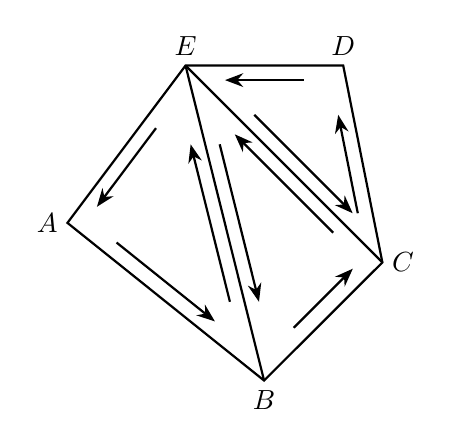
\begin{tikzpicture}
            \coordinate (A) at (0, 2.0025);
            \coordinate (B) at (2.4975, 0);
            \coordinate (C) at (4.0, 1.5);
            \coordinate (D) at (3.5025, 4.0);
            \coordinate (E) at (1.5, 4.0);

            \draw[thick] (A) -- (B) -- (C) -- (D) -- (E) -- cycle;
            \draw[thick] (B) -- (E);
            \draw[thick] (C) -- (E);

            \tikzhalflengtharrow{[xshift=-5.25pt]B}{[xshift=-5.25pt]E}
            \tikzhalflengtharrow{[xshift=5.25pt]E}{[xshift=5.25pt]B}
            \tikzhalflengtharrow{[yshift=-8.4pt]E}{[yshift=-8.4pt]A}
            \tikzhalflengtharrow{[yshift=8.4pt]B}{[yshift=8.4pt]C}
            \tikzhalflengtharrow{[yshift=7.125pt]A}{[yshift=7.125pt]B}
            \tikzhalflengtharrow{[yshift=-7.05pt]C}{[yshift=-7.05pt]E}
            \tikzhalflengtharrow{[xshift=7.05pt]E}{[xshift=7.05pt]C}
            \tikzhalflengtharrow{[yshift=-5.25pt]D}{[yshift=-5.25pt]E}
            \tikzhalflengtharrow{[xshift=-5.355pt]C}{[xshift=-5.355pt]D}

            \node[anchor=east] at (A) {\(A\)};
            \node[anchor=north] at (B) {\(B\)};
            \node[anchor=west] at (C) {\(C\)};
            \node[anchor=south] at (D) {\(D\)};
            \node[anchor=south] at (E) {\(E\)};

        \end{tikzpicture}
        \caption{A closed polygonal, chain internally triangulated.}\label{fig:cauchyintegraltheoremoversimplyconnectedset_closedpolygonalchaintriangulation}
    \end{figure}Since \(P\) is a closed polygonal chain, we can triangulate the interior. For example, consider \cref{fig:cauchyintegraltheoremoversimplyconnectedset_closedpolygonalchaintriangulation}. Then,
    \begin{align*}
        \int_{ABCDE}f(z)\ddz & =\qty(\int_{\overrightarrow{AB}}+\int_{\overrightarrow{BC}}+\int_{\overrightarrow{CD}}+\int_{\overrightarrow{DE}}+\int_{\overrightarrow{EA}})f(z)\ddz \\
        & \quad+\qty(\int_{\overrightarrow{BE}}+\int_{\overrightarrow{EB}}+\int_{\overrightarrow{CE}}+\int_{\overrightarrow{EC}})f(z)\ddz                       \\
        & =\int_{\Delta{ABE}}f(z)\ddz+\int_{\Delta{BCE}}f(z)\ddz+\int_{\Delta{CDE}}f(z)\ddz.
    \end{align*} Thus, if the integral over every triangle in \(U\) vanishes, then \cref{eq:cauchyintegraltheoremoversimplyconnectedset_statement} follows. Consider a triangle in \(U\) with boundary \(\Delta\).
    \begin{figure}
        \centering
        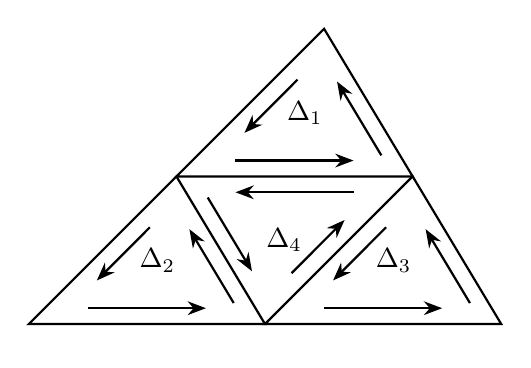
\begin{tikzpicture}
            \coordinate (A) at (0, 0);
            \coordinate (D) at (4.875, 1.875);
            \coordinate (F) at (1.875, 1.875);
            \coordinate (C) at (6, 0);
            \coordinate (B) at (3.75, 3.75);
            \coordinate (E) at (3, 0);

            \draw[thick] (A) -- (F) -- (E) -- cycle;
            \draw[thick] (B) -- (D) -- (F) -- cycle;
            \draw[thick] (C) -- (D) -- (E) -- cycle;

            \tikzhalflengtharrow{[yshift=-8.775pt]F}{[shift={(15pt, 6.15pt)}]A};
            \tikzhalflengtharrow{[yshift=-8.775pt]B}{[shift={(15pt, 6.15pt)}]F};
            \tikzhalflengtharrow{[yshift=-8.775pt]D}{[shift={(15pt, 6.15pt)}]E};
            \tikzhalflengtharrow{[yshift=8.775pt]E}{[shift={(-15pt, -6.15pt)}]D};

            \tikzhalflengtharrow{[shift={(-3.3075pt, -5.73pt)}]E}{[shift={(-3.3075pt, -5.73pt)}]F};
            \tikzhalflengtharrow{[shift={(-3.3075pt, -5.73pt)}]D}{[shift={(-3.3075pt, -5.73pt)}]B};
            \tikzhalflengtharrow{[shift={(-3.3075pt, -5.73pt)}]C}{[shift={(-3.3075pt, -5.73pt)}]D};
            \tikzhalflengtharrow{[shift={(3.3075pt, 5.73pt)}]F}{[shift={(3.3075pt, 5.73pt)}]E};

            \tikzhalflengtharrow{[yshift=5.73pt]A}{[yshift=5.73pt]E};
            \tikzhalflengtharrow{[yshift=5.73pt]E}{[yshift=5.73pt]C};
            \tikzhalflengtharrow{[yshift=5.73pt]F}{[yshift=5.73pt]D};
            \tikzhalflengtharrow{[yshift=-5.73pt]D}{[yshift=-5.73pt]F};

            \coordinate (AE) at ($(A)!0.5!(E)$);
            \coordinate (AF) at ($(A)!0.5!(F)$);
            \coordinate (FD) at ($(F)!0.5!(D)$);
            \coordinate (BF) at ($(B)!0.5!(F)$);
            \coordinate (EC) at ($(E)!0.5!(C)$);

            \path let
            \p1 = (FD),
            \p2 = (BF),
            \p3 = (AE),
            \p4 = (AF),
            \p5 = (EC)
            in
            node[shift={(3.75pt,-3.75pt)}] at (\x1, \y2) {\(\Delta_1\)}
            node[shift={(3.75pt,-3.75pt)}] at (\x3, \y4) {\(\Delta_2\)}
            node[shift={(3.75pt,-3.75pt)}] at (\x5, \y4) {\(\Delta_3\)}
            node[shift={(-3.75pt, 3.75pt)}] at (\x1, \y4) {\(\Delta_4\)};

        \end{tikzpicture}
        \caption{Quadrisection of the triangle bounded by \(\Delta\).}\label{fig:cauchyintegraltheoremoversimplyconnectedset_trianglequadrisection}
    \end{figure} Then define \(M\) to be \[M=\abs{\int_{\Delta}f(z)\ddz}.\]
    We can quadrisect the triangle bounded by \(\Delta\) into four triangles with boundaries \(\Delta_1,\Delta_2,\Delta_3,\Delta_4\) as in \cref{fig:cauchyintegraltheoremoversimplyconnectedset_trianglequadrisection}. Then one of \(\Delta_1\), \(\Delta_2\), \(\Delta_3\), or \(\Delta_4\) (denote this to be \(\Delta^1\)) satisfy
    \[\abs{\int_{\Delta^1}f(z)\ddz}\geq\frac{M}{4},\]
    and recursively, choose
    \begin{equation}
        \abs{\int_{\Delta^2}f(z)\ddz}\geq\frac{M}{4^2},\ldots,\abs{\int_{\Delta^n}f(z)\ddz}\geq\frac{M}{4^n}. \label{eq:cauchyintegraltheoremoversimplyconnectedset_trianglelowerbound}
    \end{equation}
    Let \(L\) denote the perimeter of \(\Delta\). Then, the perimeters of \(\Delta^1, \Delta^2,\ldots\) respectively are \(\frac{L}{2},\frac{L}{2^2},\ldots\). As \(n\to\infty\), \(\Delta_n\) shrinks to a single point \(z_0\). Then, \(\forall n\in\mathbb{N}\), \(z_0\in\Delta^n\).

    By the definition of holomorphy, \(\forall\varepsilon>0\), \(\exists\delta>0\) such that \(\forall z\in D\paren{z_0,\delta}\), \[\abs{\frac{f\paren{z}-f\paren{z_0}}{z-z_0}-f'\paren{z_0}}<\varepsilon,\]\[\abs{f\paren{z}-f\paren{z_0}-f'\paren{z_0}\paren{z-z_0}}<\varepsilon\abs{z-z_0},\] and \(\exists N\in\mathbb{N}\) such that \(\forall n\in \mathbb{N}_{>N}\), \(\Delta^n\subset D\paren{z_0,\delta}\). By \cref{thm:cauchyintegraltheorem}, since the functions \(z\mapsto 1\) and \(z\mapsto z\) are both entire, \[\int_{\Delta^n}\ddz=0,\quad\int_{\Delta^n}z\ddz=0.\] Then
    \begin{align*}
        \int_{\Delta^n}f(z)\ddz & =\int_{\Delta^n}f(z)\ddz-f\paren{z_0}\int_{\Delta^n}\ddz-f'\paren{z_0}\left(\int_{\Delta^n}z\ddz-z_0\int_{\Delta^n}\ddz\right) \\
        & =\int_{\Delta^n}\brackets{f(z)-f\paren{z_0}-f'\paren{z_0}\paren{z-z_0}}\ddz.
    \end{align*}
    Because the distance between any two points in the interior of a triangle is always less than its perimeter, using the triangle inequality for complex integrals, \[\int_{\Delta^n}\abs{f(z)}\abs{\ddz}\leq\varepsilon\int_{\Delta^n}\abs{z-z_0}\abs{\ddz}=\frac{\varepsilon L}{2^n}\int_{\Delta^n}\abs{\ddz}=\frac{\varepsilon L^2}{4^n}.\]
    Comparing the above equation with \cref{eq:cauchyintegraltheoremoversimplyconnectedset_trianglelowerbound}, \[\frac{M}{4^n}<\frac{\varepsilon L}{4^n},\quad M<\varepsilon L.\] Since \(\Delta\) is rectifiable, \(L\) is finite, and letting \(\varepsilon\to0\), we find that \(M\to0\). Then, for every triangle in \(U\), the integral vanishes, and \cref{eq:cauchyintegraltheoremoversimplyconnectedset_chainvanishingstatement,eq:cauchyintegraltheoremoversimplyconnectedset_chaindefinition} follow.
\end{proof}
\begin{theorem}[\textsc{Cauchy--Goursat}]\label{thm:cauchygoursattheorem}
    Let \(U\subset\mathbb{C}\) be an open region bounded with boundary \(\partial U\). Let \(f:U\to\mathbb{C}\) be a holomorphic function continuous on \(\overline{U}\). Then, \[\oint_{\partial U}f(\zeta)\ddzeta=0.\]
\end{theorem}
\begin{proof}
    Since \(\partial U\cap U=\emptyset\) and \(f(z)\) is not necessarily holomorphic over \(\overline{U}\), we cannot directly apply \cref{lem:cauchyintegraltheoremoversimplyconnectedset}.
    \begin{figure}
        \centering
        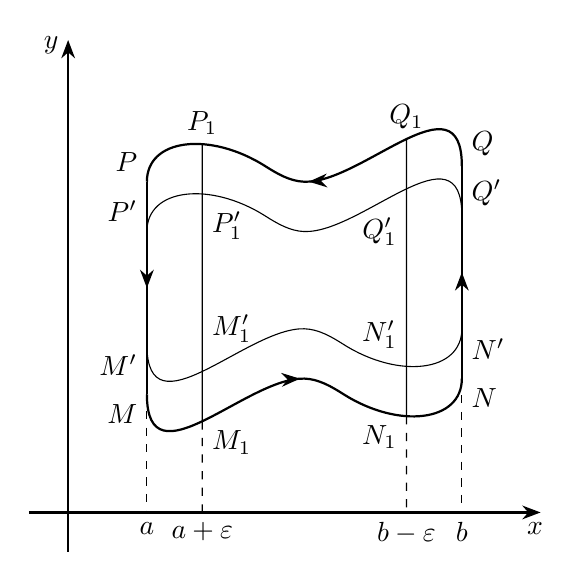
\begin{tikzpicture}[>=stealth,
                arrow style/.style={
                    postaction={decorate},
                    decoration={markings, mark=at position 0.5 with {\arrow[scale=1]{Stealth}}}
            }]
            \pgfmathsetmacro{\lengtheta}{18pt}
            \pgfmathsetmacro{\lengthepsilon}{20pt}
            \coordinate (M) at (1, 1.5);
            \coordinate (P) at (1, 4.2);
            \coordinate (Q) at (5, 4.4);
            \coordinate (N) at (5, 1.7);
            \coordinate (Mprime) at ([yshift=\lengtheta] M);
            \coordinate (Pprime) at ([yshift=-\lengtheta] P);
            \coordinate (Qprime) at ([yshift=-\lengtheta] Q);
            \coordinate (Nprime) at ([yshift=\lengtheta] N);
            \draw[-{Stealth}, thick] (-0.5, 0) -- (6, 0);
            \draw[-{Stealth}, thick] (0, -0.5) -- (0, 6);
            \draw[thick, arrow style] (P) -- (M);
            \draw[thick, arrow style, name path=curveQP] (Q) to[out angle=90, in angle=90, curve through = {([shift={(2, 0)}] P) ([shift={(1.5, 0.2)}] P)}] (P);
            \draw[thick, arrow style] (N) -- (Q);
            \draw[thick, arrow style, name path=curveMN] (M) to[out angle=270, in angle=270, curve through = {([shift={(-2, 0)}] N) ([shift={(-1.5, -0.2)}] N)}] (N);
            \path let \p1 = (P) in coordinate (P1x) at ({\x1 + \lengthepsilon}, 0);
            \path let \p1 = (Q) in coordinate (Q1x) at ({\x1 - \lengthepsilon}, 0);
            \path[name path=verticalleftmarker](P1x) -- (P1x |- 0, 6);
            \path[name path=verticalrightmarker](Q1x) -- (Q1x |- 0, 6);
            \path[name intersections={of=curveQP and verticalleftmarker, by=P1}];
            \path[name intersections={of=curveMN and verticalleftmarker, by=M1}];
            \draw[thin] (M1) -- (P1);
            \path[name intersections={of=curveQP and verticalrightmarker, by=Q1}];
            \path[name intersections={of=curveMN and verticalrightmarker, by=N1}];
            \draw[thin] (N1) -- (Q1);
            \draw[thin] (Mprime) to[out angle=270, in angle=270, curve through = {([shift={(-2, 0)}] Nprime) ([shift={(-1.5, -0.2)}] Nprime)}] (Nprime);
            \draw[thin] (Qprime) to[out angle=90, in angle=90, curve through = {([shift={(2, 0)}] Pprime) ([shift={(1.5, 0.2)}] Pprime)}] (Pprime);
            \draw[dashed] (M) -- (M |- 0, 0);
            \draw[dashed] (N) -- (N |- 0, 0);
            \draw[dashed] (M1) -- (P1x);
            \draw[dashed] (N1) -- (Q1x);
            \node[anchor=north east] at (M) {\(M\)};
            \node[anchor=south east] at (P) {\(P\)};
            \node[anchor=south west] at (Q) {\(Q\)};
            \node[anchor=north west] at (N) {\(N\)};
            \node[anchor=north east] at (Mprime) {\(M'\)};
            \node[anchor=south east] at (Pprime) {\(P'\)};
            \node[anchor=south west] at (Qprime) {\(Q'\)};
            \node[anchor=north west] at (Nprime) {\(N'\)};
            \node[anchor=north west] at (M1) {\(M_1\)};
            \node[anchor=south] at (P1) {\(P_1\)};
            \node[anchor=south] at (Q1) {\(Q_1\)};
            \node[anchor=north east] at (N1) {\(N_1\)};
            \node[anchor=south west] at ([yshift=\lengtheta+7pt] M1) {\(M'_1\)};
            \node[anchor=north west] at ([yshift=-\lengtheta-3pt] P1) {\(P'_1\)};
            \node[anchor=north east] at ([yshift=-\lengtheta-7pt] Q1) {\(Q'_1\)};
            \node[anchor=south east] at ([yshift=\lengtheta+3pt] N1) {\(N'_1\)};
            \node[anchor=north] at (M |- 0, 0) {\(a\)};
            \node[anchor=north] at (N |- 0, 0) {\(b\)};
            \node[anchor=north] at (P1x |- 0, 0) {\(a+\varepsilon\)};
            \node[anchor=north] at (Q1x |- 0, 0) {\(b-\varepsilon\)};
            \node[anchor=north, xshift=-2pt] at (6, 0) {\(x\)};
            \node[anchor=east, yshift=-2pt] at (0, 6) {\(y\)};
        \end{tikzpicture}
        \caption{A simplified region containing two vertical lines and two continuous, rectifiable curves.}
        \label{fig:cauchygoursattheorem_simplifiedregion}
    \end{figure}

    First assume \(U\) has the shape of \(MNQP\) in \cref{fig:cauchygoursattheorem_simplifiedregion}. That is, \(U\) consists of \(x=a\), \(x=b\) for \(a<b\), and two rectifiable \(C^0\) curves \(\overrightarrow{MN}:y=\varphi(x)\) and \(\overrightarrow{QP}:\psi(x)\) such that \(\varphi(x)<\psi(x)\), \(\forall a\le x\le b\).

    For some \(\varepsilon>0\), \(\eta>0\), construct a new curve \(M_1'N_1'Q_1'P_1'\in U\) to be the boundary of the region bounded by \(P_1M_1:x=a+\varepsilon\), \(N_1Q_1:b-\varepsilon\), \(M'N':\varphi(x)+\eta\), and \(Q'P': \psi(x)-\eta\) such that \(M_1'N_1'Q_1'P_1'\) remains simple. By \cref{lem:cauchyintegraltheoremoversimplyconnectedset}, \[\oint_{M_1'N_1'Q_1'P_1'}f(z)\ddz=0.\]
    By \cref{thm:heinecantor}, \(f(z)\) is uniformly continuous over \(\overline{U}\), and therefore \(\forall\varepsilon'>0\), we can choose \(\eta>0\) so that \(\forall z\in\overrightarrow{M_1'N_1'}\), \(\abs{f\paren{z}-f\paren{z-\eta}}<\varepsilon'\) is satisfied. Letting \(\eta\to0\) (with \(\varepsilon'\to0\)) and fixing \(\varepsilon>0\), we get that
    \begin{align*}
        \abs{\int_{\overrightarrow{M_1'N_1'}}f(z)\ddz-\int_{\overrightarrow{M_1N_1}}f(z)\ddz} & \leq\int_{\overrightarrow{M_1'N_1'}}\abs{f(z)-f\paren{z-\eta}}\abs{\ddz} \\
        & <\varepsilon'\int_{\overrightarrow{M_1'N_1'}}\abs{dz}\to0,
    \end{align*}
    and consequently,
    \begin{equation}
        \int_{\overrightarrow{M_1'N_1'}}f(z)\ddz\to \int_{\overrightarrow{M_1N_1}}f(z)\ddz.\label{eq:cauchygoursattheorem_innerinnerhorizontaltoouterinnerhorizontal1}
    \end{equation}
    Under the same limit, we get
    \begin{equation}
        \int_{\overrightarrow{Q_1'P_1'}}f(z)\ddz\to \int_{\overrightarrow{Q_1P_1}}f(z)\ddz.\label{eq:cauchygoursattheorem_innerinnerhorizontaltoouterinnerhorizontal2}
    \end{equation} By the continuity of \(f(z)\) over a compact set,
    \begin{equation}
        \int_{\overrightarrow{P_1'M_1'}}f(z)\ddz\to \int_{\overrightarrow{P_1M_1}}f(z)\ddz,\quad\int_{\overrightarrow{N_1'Q_1'}}f(z)\ddz\to \int_{\overrightarrow{N_1Q_1}}f(z)\ddz.\label{eq:cauchygoursattheorem_innerinnerverticaltoouterinnervertical}
    \end{equation}
    Then letting \(\varepsilon\to0\), for the same reason as \cref{eq:cauchygoursattheorem_innerinnerverticaltoouterinnervertical}, \cref{eq:cauchygoursattheorem_innerinnerhorizontaltoouterinnerhorizontal1,eq:cauchygoursattheorem_innerinnerhorizontaltoouterinnerhorizontal2} yield \[\int_{\overrightarrow{M_1N_1}}f(z)\ddz\to \int_{\overrightarrow{MN}}f(z)\ddz,\quad\int_{\overrightarrow{Q_1P_1}}f(z)\ddz\to \int_{\overrightarrow{QP}}f(z)\ddz.\]
    We are left to show the subsequent limits of the results from \cref{eq:cauchygoursattheorem_innerinnerverticaltoouterinnervertical}. For the left integral, let \(y_{\varphi}=\max\qty{\varphi(a),\varphi\paren{a+\varepsilon}}\) and \(y_{\psi}=\max\qty{\psi(a),\psi\paren{a+\varepsilon}}\).

    Then, \[\int_{\overrightarrow{PM}}f(z)\ddz=\ii\int_{\psi(a)}^{\varphi(a)}f\paren{a+\ii y}\ddy=\ii\paren{\int_{\psi(a)}^{y_\varphi}+\int_{y_\varphi}^{y_\psi}+\int_{y_\psi}^{\varphi(a)}}f(a+\ii y)\ddy.\]
    Similarly, \[\int_{\overrightarrow{P_1M_1}}f(z)\ddz=\ii\paren{\int_{\psi(a+\varepsilon)}^{y_\varphi}+\int_{y_\varphi}^{y_\psi}+\int_{y_\psi}^{\varphi(a+\varepsilon)}}f(a+\varepsilon+\ii y)\ddy.\]
    The difference \(\paren{\int_{\overrightarrow{PM}}-\int_{\overrightarrow{P_1M_1}}}f(z)\ddz\) between the two is then equal to
    \begin{gather*}
        \ii\int_{y_{\varphi}}^{y_{\psi}}\paren{f\paren{a+\ii y}-f\paren{a+\varepsilon+\ii y}}\ddz\\
        {}+{\ii\paren{\int_{\psi(a)}^{y_\varphi}+\int_{y_\psi}^{\varphi(a)}}f(a+\ii y)-\ii\paren{\int_{\psi(a+\varepsilon)}^{y_\varphi}z+\int_{y_\psi}^{\varphi\paren{a+\varepsilon}}}f(a+\varepsilon+\ii y)}.
    \end{gather*}
    The first term vanishes by uniform continuity (through the same argument used for \(M_1'N_1'\to M_1N_1\)) and the remaining four integrals all equal 0 as they are all integrable on a degenerating interval (as \(\varepsilon\to0\), \(y_\varphi\to\varphi(a)\) and \(y_\psi\to\psi(a)\) because \(\varphi, \psi\in C^0\)). Therefore, \[\int_{\overrightarrow{P_1M_1}}f(z)\ddz\to\int_{\overrightarrow{PM}}f(z)\ddz,\]
    and through similar logic, \[\int_{\overrightarrow{N_1Q_1}}f(z)\ddz\to\int_{\overrightarrow{NQ}}f(z)\ddz.\] Therefore, \[\oint_{MNQP}f(z)\ddz=0.\]
    Any open region \(U\subset\mathbb{C}\) with a simple closed boundary can be broken up into smaller regions with the same form as \(MNQP\) with finitely many auxiliary lines. Then the conclusion follows.
\end{proof}
\begin{remark}
    The theorem is also valid for any multiply connected region (and its boundary will consist of multiple curves) as a multiply connected region is equal to the union of several simply connected regions with vertical auxiliary lines between.

    Additionally, if \(U\subset\mathbb{C}\) is simply connected and \(f\) is holomorphic on \(U\), then for any two points \(z,z_0\in U\), the integral \[\int_{z_0}^z f(\zeta)\ddzeta\] is well-defined and independent of the path taken from \(z_0\) to \(z\). In this sense, a holomorphic function behaves analogously to a potential field.
\end{remark}
\begin{theorem}[\textsc{Cauchy--Goursat}]\label{thm:cauchygoursatformula}
    Let \(U\subset\mathbb{C}\) be an open region bounded with a simple closed boundary \(\partial U \), and let \(f:U\to\mathbb{C}\) be a holomorphic function continuous on \(\overline{U}\). Then for all \(z\in U\),
    \begin{equation}
        f(z)=\frac{1}{2\piup\ii}\oint_{\partial U}\frac{f(\zeta)}{\zeta-z}\ddzeta.\label{eq:cauchygoursatformula}
    \end{equation}
\end{theorem}
\begin{proof}
    By the Cauchy--Goursat Theorem (\cref{thm:cauchygoursattheorem}), \[\int_{\partial\paren{U\setminus D(z,\varepsilon)}}\frac{f(\zeta)}{\zeta-z}\ddzeta=\oint_{\partial U}\frac{f(\zeta)}{\zeta-z}\ddzeta-\oint_{\partial D(z,\varepsilon)}\frac{f(\zeta)}{\zeta-z}\ddzeta=0.\]
    From rearrangement, \[\oint_{\partial U}\frac{f(\zeta)}{\zeta-z}\ddzeta=2\piup \ii f(z)+\ii\int_0^{2\piup}\paren{f\paren{z+\varepsilon \ee^{\ii t}}-f(z)}\dd{t}.\]
    Since \(f\in C^0(\partial D(z,\varepsilon))\), as \(\varepsilon\to0\),
    \begin{align*}
        \abs{\int_0^{2\piup}\paren{f\paren{z+\varepsilon \ee^{\ii t}}-f(z)}\dd{t}} & \leq\int_0^{2\piup}\abs{f\paren{z+\varepsilon \ee^{\ii t}}-f(z)}\dd{t} \\
        & \leq2\piup\max_{t\in[0,2\piup]}\abs{f\paren{z+\varepsilon \ee^{\ii t}}-f(z)}\to0.
    \end{align*}
    By rearrangement, \[f(z)=\frac{1}{2\piup\ii}\oint_{\partial U}\frac{f(\zeta)}{\zeta-z}\ddzeta.\qedhere\]
\end{proof}
\begin{remark}
    In the proof of \cref{thm:pompeiu}, we used Lipschitz continuity for a smooth function, which was a stronger condition than necessary. The true necessity of smoothness was to be able to apply Green's Theorem (\cref{thm:complexgreen}).
\end{remark}
This profound theorem is extremely important and helpful in complex integration and essential in the evaluation of integrals, as demonstrated below.
\begin{example}\label{ex:cauchygoursatformulazeroofunity}
    Evaluate the integral \(\oint_{\partial D(0,2)}\frac{\ddz}{z^n-1}\), where \(n\in\mathbb{N}_{\geq 2}\).
\end{example}
\begin{proof}
    Since \(z^n-1=\prod_{k=0}^{n-1}\qty(z-\omega^k_n)\), where \(\omega^k_n=\ee^{\ii\piup\frac{k}{n}}\), the integrand has singularities at every \(n\)-th zero of unity. Then the integral is equal to:
    \begin{equation}
        \oint_{\partial D(0,2)}\frac{\ddz}{\prod_{j=0}^{n-1}\qty(z-\omega_j)}=\oint_{\partial D(0,2)}\sum_{j=0}^{n-1}\frac{c_j}{z-\omega_j}\ddz,\label{eq:cauchygoursatformulazerosofunity}
    \end{equation}
    where \(\cbraces{c_j}\) are the coefficients of the partial fraction decomposition. By the Cauchy--Goursat Formula (\cref{thm:cauchygoursatformula}), \cref{eq:cauchygoursatformulazerosofunity} becomes: \[\sum_{k=0}^{n-1}\oint_{\partial D(0,2)}\frac{c_k}{z-\omega_k}\ddz=2\piup\ii\sum_{k=0}^{n-1}c_k.\]
    Observe that \(\sum_{k=0}^{n-1} c_k=\lim_{z\to\infty}\sum_{k=0}^{n-1}\frac{zc_k}{z-\omega_k}=\lim_{z\to\infty}\frac{z}{z^n-1}=0\) since \(n\geq2\).
    Therefore, \[\oint_{\partial D(0,2)}\frac{\ddz}{z^n-1}=0.\qedhere\]
\end{proof}
We have also already seen the utility of parameterization via a polar transformation. Many useful identities in classical calculus can also be derived from concepts in its generalization:
\begin{example}
    Prove that \(\forall n\in\mathbb{N}\), \[\int_{0}^{2\piup}\cos^{2n}\theta\dd{\theta}=2\piup\prod_{k=1}^n\frac{2k-1}{2k}.\]
\end{example}
\begin{proof}
    Consider the integral \[\oint_{\partial\mathbb{D}}\qty(z+\frac{1}{z})^{2n}\frac{\ddz}{z}.\]
    Letting \(z=\ee^{\ii\theta}\), we get \(\oint_{\partial\mathbb{D}}\qty(\ee^{\ii\theta}+\ee^{-\ii\theta})^{2n}\ee^{-\ii\theta}\ddz=2^{2n}\ii\int_0^{2\piup}\cos^{2n}\theta\dd{\theta}\). Alternatively, we can expand the integrand and get \[\oint_{\partial\mathbb{D}}\sum_{k=0}^{2n}\binom{2n}{k}z^{2k-2n}\frac{\ddz}{z}=\sum_{k=0}^{2n}\oint_{\partial\mathbb{D}}\binom{2n}{k}z^{2k-2n-1}\ddz.\]
    When \(2k-2n-1\ge0\), the integrand is holomorphic. The integral is then equal to \[\binom{2n}{0}\oint_{\partial\mathbb{D}}z^{-2n-1}\ddz+\binom{2n}{1}\oint_{\partial\mathbb{D}}z^{-2n+1}\ddz+\cdots+\binom{2n}{n}\oint_{\partial\mathbb{D}}\frac{\ddz}{z}=2\piup\ii\binom{2n}{n},\]
    since all the higher order terms vanish:
    \[\oint_{\partial\mathbb{D}}z^{2k-2n-1}\ddz=\ii\int_0^{2\piup}\ee^{2\ii\theta(k-n)}\dd{\theta}=
        \begin{cases}
            0       &\qif* k<n \\
            2\piup\ii &\qif* k=n
    \end{cases}.\]
    Therefore, \[2^{2n}\ii\int_0^{2\piup}\cos^{2n}\theta\dd{\theta}=2\piup\ii\binom{2n}{n}\Longleftrightarrow\int_0^{2\piup}\cos^{2n}\theta\dd{\theta}=\frac{2\piup\qty(2n)!}{2^{2n}\qty(n!)^2}=\frac{2\piup\prod_{k=1}^{2n}k}{\prod_{k=1}^{n}{\qty(2k)}^2}.\]
    From simple cancellation, we get \[2\piup\frac{\prod_{k=1}^{n}\qty(2k-1)}{\prod_{k=1}^n\qty(2k)}=2\piup\prod_{k=1}^n\frac{2k-1}{2k},\]
    as expected.
\end{proof}
\begin{example}[Cauchy--Goursat Formula on the Exterior]\label{ex:cauchygoursatformulaexterior}
    Let \(\gamma\subset\mathbb{C}\) be a simple closed curve, and suppose that \(f:\mathrm{ext}(\gamma)\to\mathbb{C}\) is holomorphic and continuous on \(\overline{\mathrm{ext}(\gamma)}=\mathbb{C}\setminus\mathrm{int}(\gamma)\), where \(\mathrm{int}\) and \(\mathrm{ext}\) respectively denote the interior and exterior as in \cref{thm:jordancurve}.
    \begin{enumerate}
        \item If \(f\) has a removable singularity at \(\infty\), or if \(w=\lim_{z\to\infty} f(z)\) exists and is finite, then \(\forall z\in\mathbb{C}\setminus\gamma\), \[\frac{1}{2\piup\ii}\oint_\gamma\frac{f(\zeta)}{\zeta-z}\ddzeta=
                \begin{cases}
                    w      &\qif* z\in\mathrm{int}(\gamma) \\
                    w-f(z) &\qif* z\in\mathrm{ext}(\gamma)
            \end{cases}.\]
        \item If \(\gamma\) encloses the origin, then \(\forall z\in\mathbb{C}\setminus\gamma\), then
            \begin{equation}
                \frac{1}{2\piup\ii}\oint_\gamma\frac{zf(\zeta)}{z\zeta-\zeta^2}\ddzeta=
                \begin{cases}
                    0    &\qif* z\in\mathrm{int}(\gamma)                                                       \\
                    f(z) &\qif* z\in\mathrm{ext}(\gamma)\label{eq:cauchygoursatformulaexteriorpart2_statement}
                \end{cases}.
            \end{equation}
    \end{enumerate}
\end{example}
\begin{proof}
    \begin{enumerate}
        \item By the compactness of \(\gamma\), it can be completely contained within a sufficiently large disk centered at the origin (\(\gamma\subset D(0,R)\)). Then by applying \cref{thm:cauchygoursatformula} or \cref{thm:cauchygoursattheorem} on the set \(D(0,R)\cap\mathrm{ext}(\gamma)=D(0,R)\setminus\overline{\mathrm{int}(\gamma)}\), we get that \[\frac{1}{2\piup\ii}\oint_{\partial D(0,R)}\frac{f(\zeta)}{\zeta-z}\ddzeta=\frac{1}{2\piup\ii}\oint_\gamma\frac{f(\zeta)}{\zeta-z}\ddzeta+
                \begin{cases}
                    0    &\qif* z\in\mathrm{int}(\gamma)            \\
                    f(z) &\qif* z\in D(0,R)\cap\mathrm{ext}(\gamma)
            \end{cases}.\]
            By letting \(R\to\infty\) and letting \(\zeta=R\ee^{\ii\theta}\), we get that \[\frac{1}{2\piup\ii}\oint_\gamma\frac{f(\zeta)}{\zeta-z}\ddzeta=\frac{1}{2\piup}\lim_{R\to\infty}\int_0^{2\piup}\frac{f\qty(R\ee^{\ii\theta})}{1-\frac{z}{R\ee^{\ii\theta}}}\dd{\theta}-
                \begin{cases}
                    0    &\qif* z\in\mathrm{int}(\gamma) \\
                    f(z) &\qif* z\in\mathrm{ext}(\gamma)
            \end{cases}.\]
            By the continuity of \(f\) on \(\partial D(0,R)\), it attains its maximum \(M\). For sufficiently large \(R\), \(\abs{1-\frac{z}{R\ee^{\ii\theta}}}\) attains a positive minimum. Then the integrand is uniformly bounded in \(R\) and \(\theta\), and hence the order of the limit and the integral may be exchanged. Hence,
            \begin{align*}
                \frac{1}{2\piup\ii}\oint_\gamma\frac{f(\zeta)}{\zeta-z}\ddzeta & =\frac{1}{2\piup}\int_0^{2\piup}\frac{w}{1-\lim_{R\to\infty}\frac{z}{R\ee^{\ii\theta}}}\dd{\theta}-
                \begin{cases}
                    0    &\qif* z\in\mathrm{int}(\gamma) \\
                    f(z) &\qif* z\in\mathrm{ext}(\gamma)
                \end{cases}                                                                                                                               \\   & =
                \begin{cases}
                    w      &\qif* z\in\mathrm{int}(\gamma) \\
                    w-f(z) &\qif* z\in\mathrm{ext}(\gamma)
                \end{cases},
            \end{align*} as expected.
        \item Under the partial fraction decomposition of \cref{eq:cauchygoursatformulaexteriorpart2_statement}, we get that
            \begin{align}
                I & =\oint_\gamma\frac{zf(\zeta)}{z\zeta-\zeta^2}\ddzeta=\oint_\gamma\qty(\frac{f(\zeta)}{\zeta}-\frac{f(\zeta)}{\zeta-z})\ddzeta\nonumber \\
                & =\int_0^{2\piup}\qty(f\qty(R\ee^{\ii\theta})-\frac{f\qty(R\ee^{\ii\theta})}{1-\frac{z}{R\ee^{\ii\theta}}})\dd{\theta}+
                \begin{cases}
                    0            &\qif* z\in\mathrm{int}(\gamma)            \\
                    2\piup\ii f(z) &\qif* z\in\mathrm{ext}(\gamma)\cap D(0,R),
                \end{cases}\label{eq:cauchygoursatformulaexteriorpart2_prelimitintegral}
            \end{align} when \(\gamma\subset D(0,R)\).
            We will analyze the first integral as \(R\to\infty\). By the triangle and reverse triangle inequalities,
            \begin{align*}
                \qty|\int_0^{2\piup}\qty(f\qty(R\ee^{\ii\theta})-\frac{f\qty(R\ee^{\ii\theta})}{1-\frac{z}{R\ee^{\ii\theta}}})\dd{\theta}| & \leq\int_0^{2\piup}\qty|\frac{z}{R\ee^{\ii\theta}-z}|\dd{\theta}           \\
                & \leq\int_0^{2\piup}\frac{\abs{z}}{R-\abs{z}}\dd{\theta}=\frac{2\piup\abs{z}}{R-\abs{z}}\to0.
            \end{align*}
    \end{enumerate}
    By substituting the result into \cref{eq:cauchygoursatformulaexteriorpart2_prelimitintegral}, and letting \(R\to\infty\), we get that \[\frac{1}{2\piup\ii}\oint_\gamma\frac{zf(\zeta)}{z\zeta-\zeta^2}\ddzeta=
        \begin{cases}
            0    &\qif* z\in\mathrm{int}(\gamma) \\
            f(z) &\qif* z\in\mathrm{ext}(\gamma)
    \end{cases},\] as desired.
\end{proof}
\subsection{Analyticity and Holomorphy}\label{sec:analyticityandholomorphy}
The Cauchy--Goursat Formula (\cref{thm:cauchygoursatformula}) can also be generalized into a result that equates complex integration and differentiation:
\begin{theorem}[\textsc{Cauchy--Goursat}]\label{thm:cauchydifferentiationformula}
    Let \(U\subset\mathbb{C}\) be an open region bounded by a simple closed boundary \(\partial U\), and let \(f:U\to\mathbb{C}\) be holomorphic and continuous over \(\overline{U}\). Then \(\forall z\in U\), \(\forall n\in\mathbb{N}\), \(f^{(n)}(z)\) exists, and
    \begin{equation}
        f^{(n)}(z)=\frac{n!}{2\piup\ii}\oint_{\partial U}\frac{f(\zeta)}{\paren{\zeta-z}^{n+1}}\ddzeta.\label{eq:cauchydifferentiationformula_statement}
    \end{equation}
    Additionally, since \(U\) is open, \(\forall z_0\in U\), \(\forall r>0\) such that the closed disk \(\overline{D\paren{z_0,r}}\subset U\), \(f\) has the uniformly and absolutely convergent Taylor expansion
    \begin{equation}
        f(z)=\sum_{j=0}^\infty a_j\paren{z-z_0}^j,\label{eq:cauchydifferentiationformula_taylorseries}
    \end{equation}
    where
    \begin{equation}
        a_j=\frac{1}{2\piup\ii}\oint_{\partial U}\frac{f(\zeta)}{\paren{\zeta-z}^{j+1}}\ddzeta\label{eq:cauchydifferentiationformula_taylorseriescoefficients}
    \end{equation} on \(\overline{D\paren{z_0,r}}\).
\end{theorem}
\begin{proof}
    \(\forall z_0\in U\), \(\forall z\in D\paren{z_0,r}\subset U\), by \cref{thm:cauchygoursatformula}, \[f(z)-f\paren{z_0}=\frac{1}{2\piup\ii}\oint_{\partial U}\paren{\frac{f(\zeta)}{\zeta-z}-\frac{f(\zeta)}{\zeta-z_0}}\ddzeta=\frac{z-z_0}{2\piup\ii}\oint_{\partial U}\frac{f(\zeta)\ddzeta}{\paren{\zeta-z}\paren{\zeta-z_0}},\]
    and dividing by \(z-z_0\), the above is equal to \[\frac{f(z)-f\paren{z_0}}{z-z_0}=\frac{1}{2\piup\ii}\oint_{\partial U}\frac{f(\zeta)\ddzeta}{\paren{\zeta-z}\paren{\zeta-z_0}}.\]
    Since
    \begin{align}
        \frac{f(z)-f\paren{z_0}}{z-z_0}-\frac{1}{2\piup\ii}\oint_{\partial U}\frac{f(\zeta)\ddzeta}{\paren{\zeta-z_0}^2} & =\frac{1}{2\piup\ii}\oint_{\partial U}\frac{f\paren{\zeta}}{\zeta-z_0}\paren{\frac{1}{\zeta-z}-\frac{1}{\zeta-z_0}}\ddzeta\nonumber                                      \\
        & =\frac{z-z_0}{2\piup\ii}\oint_{\partial U}\frac{f(\zeta)}{(\zeta-z)\paren{\zeta-z_0}^2}\ddzeta.\label{eq:cauchydifferentiationformula_differenceoffirstorderdifferences}
    \end{align}
    Let \(d\) be the distance from \(z_0\) to \(\partial U\), and it follows that \(0<r<d\). Then, since \(\abs{z-z_0}<r\) and \(\abs{\zeta-z_0}\geq d\), \(\abs{\zeta-z}\geq d-r\). Then the absolute value of the integrand of \cref{eq:cauchydifferentiationformula_differenceoffirstorderdifferences} is bounded above by \(\frac{M}{d^2(d-r)}\), where \(M\) is the maximum of \(f(\zeta)\), which exists by \cref{thm:continuousfunctionboundedoncompact}. Then, \[\abs{\frac{z-z_0}{2\piup\ii}\oint_{\partial U}\frac{f(\zeta)}{(\zeta-z)\paren{\zeta-z_0}^2}\ddzeta}\leq\frac{\abs{z-z_0}}{2\piup}\frac{M}{d^2(d-r)}\oint_{\partial U}\abs{\ddzeta}.\] As \(z\to z_0\), the difference vanishes, and therefore, \[f'\paren{z_0}=\frac{1}{2\piup\ii}\oint_{\partial U}\frac{f(\zeta)}{\paren{\zeta-z_0}^2}\ddzeta.\]
    Now inductively assume that \cref{eq:cauchydifferentiationformula_statement} is true for a given \(n=k\in\mathbb{N}\), or \[f^{(k)}(z)=\frac{k!}{2\piup\ii}\oint_{\partial U}\frac{f(\zeta)}{\paren{\zeta-z}^{k+1}}\ddzeta.\]
    Notice the expansion of the kernel, convergent since \(\abs{z-z_0}<\abs{\zeta-z_0}\):
    \begin{equation}
        \frac{1}{\zeta-z}=\frac{1}{\zeta-z_0}\cdot\frac{\zeta-z_0}{\zeta-z}=\frac{1}{\zeta-z_0}\cdot\frac{1}{1-\frac{z-z_0}{\zeta-z_0}}=\frac{1}{\zeta-z_0}\sum_{j=0}^{\infty}\paren{\frac{z-z_0}{\zeta-z_0}}^j.\label{eq:cauchydifferentiationformula_kernelexpansion}
    \end{equation}
    Then,
    \begin{align*}
        f^{(k)}(z) & =\frac{k!}{2\piup\ii}\oint_{\partial U}\frac{f(\zeta)}{(\zeta-z)^{k+1}}\ddzeta                                                                           \\
        & =\frac{k!}{2\piup\ii}\oint_{\partial U}\frac{f(\zeta)}{\paren{\zeta-z_0}^{k+1}}\paren{\sum_{j=0}^{\infty}\paren{\frac{z-z_0}{\zeta-z_0}}^j}^{k+1}\ddzeta \\
        & =f^{(k)}\paren{z_0}+\frac{(k+1)!\paren{z-z_0}}{2\piup\ii}\oint_{\partial U}\frac{f(\zeta)}{\paren{\zeta-z_0}^{k+2}}\ddzeta                               \\
        & \quad+\order{\abs{z-z_0}^2},
    \end{align*}
    where the remainder terms \(\order{\abs{z-z_0}^2}\) resemble
    \[\paren{z-z_0}^2\frac{k!}{2\piup\ii}\brackets{k+1+\binom{k+1}{2}}\oint_{\partial U}\frac{f(\zeta)}{\paren{\zeta-z_0}^{k+3}}\ddzeta+\order{\abs{z-z_0}^3}.\]
    The difference quotient is equal to \[\frac{f^{(k)}(z)-f^{(k)}\paren{z_0}}{z-z_0}=\frac{(k+1)!}{2\piup\ii}\oint_{\partial U}\frac{f(\zeta)}{\paren{\zeta-z_0}^{k+2}}\ddzeta+\order{\abs{z-z_0}}.\] As \(z\to z_0\), the remainder terms vanish, and \[f^{(k+1)}\paren{z_0}=\frac{(k+1)!}{2\piup\ii}\oint_{\partial U}\frac{f(\zeta)}{\paren{\zeta-z_0}^{k+2}}\ddzeta.\]
    By induction, \cref{eq:cauchydifferentiationformula_statement} is valid. By substituting \cref{eq:cauchydifferentiationformula_kernelexpansion} into \eqref{eq:cauchygoursatformula}, we obtain \[f(z)=\frac{1}{2\piup\ii}\oint_{\partial U}\frac{f(\zeta)}{\zeta-z_0}\sum_{j=0}^{\infty}\paren{\frac{z-z_0}{\zeta-z_0}}^j\ddzeta=\frac{1}{2\piup\ii}\oint_{\partial U}\sum_{j=0}^{\infty}\paren{z-z_0}^j\frac{f(\zeta)\ddzeta}{\paren{\zeta-z_0}^{j+1}}.\]
    Because \(f(\zeta)\) is continuous over \(\partial U\), it is bounded by a constant \(M\). Additionally, since \(\abs{z-z_0}<\abs{\zeta-z_0}\), the sum is termwise bounded by the convergent series \[\sum_{j=0}^\infty\frac{Mr^j}{\inf_{\xi\in\partial U}\abs{\xi-z_0}^{j+1}}.\]
    By the Weierstrass \(M\)--Test (\cref{thm:weierstrassmtest}), the series uniformly converges, and we can justify
    \begin{gather*}
        \frac{1}{2\piup\ii}\oint_{\partial U}\sum_{j=0}^{\infty}\paren{z-z_0}^j\frac{f(\zeta)}{\paren{\zeta-z_0}^{j+1}}\ddzeta=\frac{1}{2\piup\ii}\sum_{j=0}^{\infty}\oint_{\partial U}\paren{z-z_0}^j\frac{f(\zeta)}{\paren{\zeta-z_0}^{j+1}}\ddzeta\\=\sum_{j=0}^\infty a_j\paren{z-z_0}^j,
    \end{gather*}
    which verifies \cref{eq:cauchydifferentiationformula_taylorseries,eq:cauchydifferentiationformula_taylorseriescoefficients}.
\end{proof}
\begin{remark}
    By induction, we have shown that assuming the existence of the first order derivative of a holomorphic function \(f\), the \(n\)-th order derivative of \(f\) exists \(\forall n\in\mathbb{N}\) and is holomorphic over the same region as \(f^{(n-1)}\). Furthermore, if \(f\) is holomorphic, then \(\forall z\in U\), there exists an open disk enclosing \(z\) such that \(f\) has a convergent Taylor series expansion. This property is known as \textscsl{analyticity}, and \cref{thm:cauchydifferentiationformula} tells us that all holomorphic functions are analytic. Analytic functions can be expanded into power series, which are termwise differentiable, and therefore complex differentiable. Thus, analyticity and holomorphy are logically equivalent, which is a fundamental difference between real and complex functions.
\end{remark}
The differentiation formula above can be thought of as a generalization of \cref{thm:cauchygoursatformula}, and provides similar utility in the evaluation of integrals:
\begin{example}\label{ex:legendrepolynomialintegralformula}
    A \textscsl{Legendre polynomial} is a polynomial whose explicit equation is given by
    \begin{equation}
        P_n(z)=\frac{1}{2^n n!}\dv[n]{z}({\qty(z^2-1)}^n).\label{eq:legendrepolynomialintegralformula_rodriguesformula}
    \end{equation}
    Prove the integral form \[P_n(z)=\frac{1}{2\piup\ii}\oint_\gamma\frac{{\qty(\zeta^2-1)}^n}{2^n{(\zeta-z)}^{n+1}}\ddzeta,\] where \(\gamma\) is a simple closed curve enclosing \(z\).
\end{example}
\begin{proof}
    By applying Cauchy--Goursat (\cref{thm:cauchydifferentiationformula}) on \cref{eq:legendrepolynomialintegralformula_rodriguesformula}, we get that \[P_n(z)=\frac{1}{2^{n+1}\piup \ii}\oint_{\gamma}\frac{{\qty(\zeta^2-1)}^n}{{(\zeta-z)}^{n+1}}\ddzeta,\] as desired.
\end{proof}
\begin{theorem}[\textsc{Cauchy's Estimate}]\label{thm:cauchysestimate}
    For a function \(f:U\to\mathbb{C}\) holomorphic over \(U\subseteq\mathbb{C}\) and \(\forall z_0\in U\) and \(\forall R>0\) such that \(\overline{D\paren{z_0,R}}\subseteq{U}\), \(\forall n\in\mathbb{N}\), \[\abs{f^{(n)}\paren{z_0}}\leq\frac{n!M}{R^n},\]
    where \[M=\max_{z\in\overline{D\paren{z_0,R}}}\abs{f(z)}.\]
\end{theorem}
\begin{proof}
    By the Differentiation Formula (\cref{thm:cauchydifferentiationformula}), \(\forall n\in\mathbb{N}\), \[f^{(n)}\paren{z_0}=\frac{n!}{2\piup\ii}\oint_{\partial D\paren{z_0,R}}\frac{f(\zeta)}{\paren{\zeta-z_0}^{n+1}}\ddzeta.\]
    Because \(f(z)\) is continuous over the boundary \(\partial D\paren{z_0,R}\), it is bounded by \(M\). Thus,
    \[\abs{f^{(n)}\paren{z_0}}\leq\frac{n!}{2\piup}\int_0^{2\piup}\frac{M}{\paren{\ee^{\ii\theta}R}^{n+1}}\ee^{\ii\theta}R\dd{\theta}=\frac{n!M}{R^n},\] as desired.
\end{proof}
\cref{thm:nthderivativeboundedl1norm} will profoundly generalize this statement significantly. The relationship between the derivatives of a holomorphic function and the function itself is an important property of holomorphic functions.
\begin{example}
    Let \(f\) be entire and \(\forall z\in\mathbb{C}\), \(|f(z)|\leq M\ee^{\abs{z}}\). Prove that \(\forall n\in\mathbb{N}\), \(|f(0)|\leq M\) and \[\abs{f^{(n)}(0)}\leq Mn!\qty(\frac{\ee}{n})^n.\]
\end{example}
\begin{proof}
    \(|f(0)|\leq M\) is obviously true by letting \(z=0\). Then \(\forall R>0\), by Cauchy's Estimate (\cref{thm:cauchysestimate}), \[\abs{f^{(n)}(0)}\leq Mn!\frac{\ee^{R}}{R^n}.\]
    By letting \(R=n\), the conclusion follows. In fact, this is the tightest possible inequality. Consider \(\varphi(R)=Mn!\frac{\ee^R}{R^n}\) to be a function of \(R\). It attains its minimum as its derivative vanishes:
    \[\varphi'(R)=Mn!\frac{\ee^RR^n-n\ee^RR^{n-1}}{R^{2n}}=0\Longleftrightarrow R^n=nR^{n-1}\Longleftrightarrow R=n.\] To confirm it as a minimum, we calculate the second order derivative:
    \[\varphi''(R)=Mn!\ee^R\qty(\frac{1}{R^n}-\frac{2n}{R^{n+1}}+\frac{n(n+1)}{R^{n+2}})\Longrightarrow\varphi''(n)=M(n-1)!\frac{\ee^n}{n^n},\]
    which is positive and convex.
\end{proof}
The following theorem, albeit originally proven by Cauchy in 1844, shows a fundamental difference between holomorphic functions on proper subsets of \(\mathbb{C}\) and entire functions.
\begin{theorem}[\textsc{Liouville}]\label{thm:liouville}
    Any bounded entire function is constant.
\end{theorem}
\begin{proof}
    Let \(f:\mathbb{C}\to\mathbb{C}\) be entire. Then, \(\forall z_0\in\mathbb{C}\), \(\forall R>0\), \(f\) is holomorphic over \(\overline{D\paren{z_0,R}}\). By \cref{thm:cauchysestimate}, \[\abs{f'\paren{z_0}}\leq\frac{M}{R},\] where \(M=\sup_{z\in\mathbb{C}}\abs{f(z)}\). By letting \(R\to\infty\), \(f'\paren{z_0}\) where \(z_0\) is any arbitrary value in \(\mathbb{C}\). Therefore, \(f(z)\) is constant.

    Alternatively, let \(a,b\in\mathbb{C}\) be distinct and arbitrarily chosen. Let \(f:\mathbb{C}\to\mathbb{C}\) be entire and bounded such that \(\abs{f}\leq M\) for some \(M>0\). Let \(R>\abs{a},\abs{b}\). Since \(a\neq b\), \(\exists\varepsilon>0\) such that \(\overline{D(a,\varepsilon)}\cup\overline{D(b,\varepsilon)}=\emptyset\). By the Cauchy--Goursat Theorem (\cref{thm:cauchygoursattheorem}), we have \[\oint_{\partial D(0,R)}\frac{f(z)}{(z-a)(z-b)}\ddz=\qty(\oint_{\partial D(a,\varepsilon)}+\oint_{\partial D(b,\varepsilon)})\frac{f(z)}{(z-a)(z-b)}\ddz.\]
    Since \(z\mapsto\frac{f(z)}{z-a}\) is holomorphic on the disk centered at \(b\) and \(z\mapsto\frac{f(z)}{z-b}\) is holomorphic on the disk centered at \(a\), by the Cauchy--Goursat Formula (\cref{thm:cauchygoursatformula}), we have \[\oint_{\partial D(0,R)}\frac{f(z)}{(z-a)(z-b)}\ddz=2\piup\ii\qty(\frac{f(b)}{b-a}+\frac{f(a)}{a-b}).\]
    On the contrary, we also have
    \begin{align*}
        \abs{\qty(\oint_{\partial D(a,\varepsilon)}+\oint_{\partial D(b,\varepsilon)})\frac{f(z)}{(z-a)(z-b)}\ddz} & \leq M\oint_{\partial D(0,R)}\frac{\abs{\ddz}}{\abs{z-a}\abs{z-b}} \\
        & =\frac{2\piup MR}{(R-a)(R-b)}                                       \\
        & \to 0\qas{R\to\infty}.
    \end{align*}
    We conclude that \[\frac{2\piup\ii}{b-a}\qty(f(b)-f(a))=0\] for all distinct complex \(a\) and \(b\). Hence, \(f\) is a constant function.
\end{proof}
\begin{theorem}[\textsc{Morera}]\label{thm:morera}
    Let \(U\subseteq\mathbb{C}\) and \(f:U\to\mathbb{C}\) be continuous over \(U\). If for any rectifiable closed curve \(\gamma\subset U\), \[\oint_{\gamma}f(\zeta)\ddzeta=0,\] then \(f\) is holomorphic over \(U\).
\end{theorem}
\begin{proof}
    Since the integral vanishes on any closed curve \(\gamma\), \(\forall z_0,z\in U\), the integral is path independent with endpoints \(z_0\) and \(z\):
    \[F(z)=\int_{z_0}^zf(\zeta)\ddzeta.\]
    As \(f(z)\) is continuous over \(U\), \(F(z)\) is continuous over \(U\) as well. \(F(z)\) is holomorphic over \(U\) (complex differentiable with \(F'(z)=f(z)\)), and by \cref{thm:cauchydifferentiationformula}, the derivative of \(F(z)\), \(f(z)\) is also holomorphic over \(U\).
\end{proof}
\begin{theorem}\label{thm:nthderivativeboundedl1norm}
    Let \(U\subseteq\mathbb{C}\) be open, let \(K\subset U\) be compact and \(V\supset K\) be open such that \(\overline{V}\subset U\) (\(V\) is a neighborhood of \(K\) that is relatively compact in \(U\)). Let \(f(z)\) be holomorphic in \(U\). Then there exists a sequence \(\cbraces{c_n}\subset\mathbb{R}\) dependent only on \(K\) and \(V\) (independent of \(f\) and \(z\)) such that \(\forall n\in\mathbb{N}\),
    \begin{equation}
        \sup_{z\in K}\abs{f^{(n)}(z)}\leq c_n\left\|f\right\|_{L^1(V)},\label{eq:nthderivativeboundedl1norm_statement}
    \end{equation}
    where \(\norm{f}_{L^p(V)}\) denotes \[\paren{\int_V\abs{f(z)}^p\ddx\wedge\ddy}^{\flatfrac{1}{p}}.\]
\end{theorem}
\begin{proof}
    Let \(\varphi\in C^\infty\paren{\mathbb{C}}\)  satisfy \(\supp(\varphi)\subset V\) and be identically equal to 1 over some open neighborhood \(W\) of \(K\) relatively compact in \(V\). Since \(f\in C^\infty\paren{U}\), by the Cauchy--Pompeiu Theorem (\cref{thm:pompeiu}) on \(f(z)\varphi(z)\in C^\infty\paren{\overline{U}}\), \[f(z)\varphi(z)=\frac{1}{2\piup\ii}\paren{\int_{\partial U}\frac{f(\zeta)\varphi(\zeta)}{\zeta-z}\ddzeta-\int_{U}\pdv{f(\zeta)\varphi(\zeta)}{\overline{\zeta}}\cdot\frac{\dd{\overline{\zeta}}\wedge\ddzeta}{\zeta-z}}.\]
    By the product rule, \[\pdv{f(\zeta)\varphi(\zeta)}{\overline{\zeta}}=\pdv{\varphi(\zeta)}{\overline{\zeta}}f(\zeta),\] and since \(\partial U\subset\mathbb{C}\setminus\supp(\varphi)\), the first term vanishes, resulting in \[f(z)\varphi(z)=-\frac{1}{2\piup\ii}\int_U\pdv{\varphi(\zeta)}{\overline{\zeta}}f(\zeta)\cdot\frac{\dd{\overline{\zeta}}\wedge\ddzeta}{\zeta-z}.\] Let \(K_1\) denote \(\supp\paren{\pdv{\varphi(\zeta)}{\overline{\zeta}}}\), and \(\forall z\in K\), \(\varphi(z)=1\). Therefore, \[f(z)=\frac{1}{2\piup\ii}\int_{K_1}f(\zeta)\cdot\pdv{\varphi(\zeta)}{\overline{\zeta}}\cdot\frac{\ddzeta\wedge\dd{\overline{\zeta}}}{\zeta-z}.\]
    We can differentiate within the integral as \(f(\zeta)\cdot\pdv{\varphi(\zeta)}{\overline{\zeta}}\) is \(C^\infty\) and bounded over \(K_1\), and thus the integrand is uniformly bounded by an integrable function independent of \(\zeta\):
    \[f^{(n)}(z)=\frac{n!}{2\piup\ii}\int_{K_1} f(\zeta)\cdot\pdv{\varphi(\zeta)}{\overline{\zeta}}\cdot\frac{\ddzeta\wedge\dd{\overline{\zeta}}}{\paren{\zeta-z}^{n+1}},\]
    and by the triangle inequality,
    \[\abs{f^{(n)}(z)}\leq\frac{n!}{2\piup}\int_{K_1} \abs{f(\zeta)}\abs{\pdv{\varphi(\zeta)}{\overline{\zeta}}}\frac{\abs{\ddzeta\wedge\dd{\overline{\zeta}}}}{\abs{\zeta-z}^{n+1}}.\]
    Notice that over \(W\), \(\varphi=1\), \(\varphi'=0\), and is disjoint from \(K_1\) (or that \(W\cap K_1=\emptyset\)). Then, the distance between \(W\) and \(K\) is positive and the two are disjoint. Therefore, \(\exists M>0\) such that
    \[\frac{1}{\abs{\zeta-z}}\leq M,\] and thus, \[\abs{\pdv{\varphi(\zeta)}{\overline{\zeta}}}\frac{1}{\abs{\zeta-z}^{n+1}}\] can be bounded by a sequence \(\cbraces{c'_n}\), independent of \(f\) and dependent only on \(n\) and the sets \(K\) and \(V\). Then, \[\abs{f^{(n)}(z)}\leq\frac{n!}{2\piup}\int_{K_1}c'_n\abs{f(\zeta)}{\abs{\ddzeta\wedge\dd{\overline{\zeta}}}}=\frac{n!}{\piup}\int_{K_1}c'_n\abs{f(\zeta)}{\abs{\ddx\wedge\ddy}}.\] Because \(K_1\) is compact, it has a finite area \(\mathrm{area}\qty(K_1)\), and we can define a new sequence \(c_n=\frac{n!}{\piup}c'_n\mathrm{area}\qty(K_1)\) to find that \[\abs{f^{(n)}(z)}\leq c_n\int_{K_1}\abs{f(\zeta)}{\abs{\ddx\wedge\ddy}}\leq c_n\int_{V}\abs{f(\zeta)}{\abs{\ddx\wedge\ddy}}.\]

    The problem now stands to prove that \(\varphi(z)\) exists in the first place, which requires a topological argument to be later discussed in \cref{thm:bumpfunctionexistence}.
\end{proof}
\begin{corollary}\label{cor:nthderivativeboundedsupremum}
    Let \(U\subseteq\mathbb{C}\) be open, let \(K\subset U\) be compact and \(V\supset K\) be open such that \(\overline{V}\subset U\). For any holomorphic function \(f(z)\) in \(U\), there exist constants (independent of \(z\) and \(f\)) \(\cbraces{c_n}\) such that \[\sup_{z\in K}\abs{f^{(n)}(z)}\leq c_n\sup_{z\in V}\abs{f(z)}.\]
\end{corollary}
\begin{proof}
    Starting from \cref{eq:nthderivativeboundedl1norm_statement}, observe that \[c_n\left\|f\right\|_{L^1(V)}\leq c_n\mathrm{area}(V)\sup_{z\in V}\abs{f(z)},\] and we can define a new set of constants equal to \(c_n\mathrm{area}(V)\), which are still independent of \(z\).
\end{proof}
For the next theorem we will briefly introduce the concept of \textscsl{analytic continuation}.
\begin{definition}[Analytic Continuation]\label{def:analyticcontinuation}
    Let \(U\subseteq\mathbb{C}\) be open, and let \(f:U\to\mathbb{C}\) be holomorphic. Let \(V\subseteq\mathbb{C}\) be open with \(U\subseteq V\). A function
    \(F:U\cap V\to\mathbb{C}\) is an \textscsl{analytic continuation} of \(f\) to \(V\) if:
    \begin{enumerate}
        \item \(F\) is holomorphic on \(V\), and
        \item \(F\equiv f\) on \(U\).
    \end{enumerate}
\end{definition}
The concept of analytic continuation and its consequent problems and properties will be discussed in more detail in \cref{sec:analyticcontinuation}. For now, we will prove a theorem that is a direct consequence of the Cauchy--Goursat Differentiation Formula (\cref{thm:cauchydifferentiationformula}) and the existence of holomorphic functions with removable singularities.
\begin{theorem}[Riemann]\label{thm:riemannremovablesingularities}
    Let \(D^*\qty(z_0,r)=D\paren{z_0,r}\setminus\cbraces{z_0}\) (known as a punctured disk), and \(f:D^*\paren{z_0,r}\to\mathbb{C}\) be holomorphic and bounded. Then \(f\) can be analytically continued to \(D\paren{z_0,r}\).
\end{theorem}
\begin{proof}
    Define the auxiliary function \[\varphi(z)=
        \begin{cases}
            \paren{z-z_0}^2f(z) &\qif* z\in D^*\paren{z_0,r} \\
            0                   &\qif* z=z_0
    \end{cases}.\]
    \(\varphi(z)\) is bounded and continuously differentiable on \(D\paren{z_0,r}\) and satisfies the Cauchy--Riemann Equations since
    \[\lim_{z\to z_0}\frac{\varphi(z)-\varphi\paren{z_0}}{z-z_0}=\frac{\paren{z-z_0}^2f(z)}{z-z_0}=\lim_{z\to z_0}\paren{z-z_0}f(z)=0,\] meaning that \(\dv{\varphi}{z}\paren{z_0}=0\). For \(z\in D^*\paren{z_0,r}\), \[\varphi'(z)=2\paren{z-z_0}f(z)+\paren{z-z_0}^2f'(z).\] As \(z\to z_0\), \(\varphi(z)\to0\), meaning that \(\varphi\) is holomorphic over \(D\paren{z_0,r}\). By \cref{thm:cauchydifferentiationformula}, \[\varphi(z)=\sum_{j=2}^\infty a_j\paren{z-z_0}^j,\]
    which is convergent over \(D\paren{z_0,r}\). Then we can define \[\widetilde{f}(z)=\frac{\varphi(z)}{\paren{z-z_0}^2}=\sum_{j=0}^\infty a_{j+2}\paren{z-z_0}^j\] over the same disk of convergence. Over the punctured disk, \(\widetilde{f}(z)=f(z)\), and therefore \(\widetilde{f}\) is an analytic continuation of \(f\).
\end{proof}
\subsubsection{Partitions of Unity and the Existence of Bump Functions}
\begin{definition}[Topological Space]
    A \textscsl{topological space} is a pair \((X, \tau)\), where \(X\) is a set and \(\tau\) is a collection of subsets of \(X\) satisfying the following properties:
    \begin{enumerate}
        \item \(\emptyset\in\tau\) and \(X\in\tau\),
        \item The union of any collection of sets in \(\tau\) is also in \(\tau\),
        \item The intersection of any finite number of sets in \(\tau\) is also in \(\tau\).
    \end{enumerate}
    The collection \(\tau\) is called a \textscsl{topology} on \(X\), and its elements are referred to as \textscsl{open sets} under the topology \(\tau\).
\end{definition}
If a topological space \(X\) can be written as the union between two nonempty disjoint open sets, then it is \textscsl{disconnected}. Otherwise, it is \textscsl{connected}.

A topology allows the definition and general conceptualization of continuity, convergence, and connectivity in a general setting, without necessarily relying on a notion of distance (a metric).

For example, in a topological space, a function \(f:X\to Y\) between two topological spaces is said to be continuous if the preimage of every open set in \(Y\) is an open set in \(X\). This generalizes the familiar \(\varepsilon\)-\(\delta\) definition of continuity from calculus.
\begin{example}
    To illustrate this, consider the function \(f:\mathbb{R} \to \mathbb{R}\) defined by
    \[f(x)=
        \begin{cases}
            1 &\qif* x\geq0, \\
            0 &\qif* x<0.
        \end{cases}
    \]
    We equip both the domain and codomain with the standard topology on \(\mathbb{R}\).
    Let \(V=(0.5,1.5)\subseteq\mathbb{R}\). Then the preimage of \(V\) is \[f^{-1}(V)=\cbraces{x\in\mathbb{R}}{f(x)\in(0.5,1.5)}=[0,\infty),\]
    which is not an open set in the standard topology on \(\mathbb{R}\).
\end{example}
\begin{definition}[Basis of a Topology]
    For a topological space \((X,\tau)\), a \textscsl{basis} \(\mathfrak{B}\subseteq\tau\) is a subcollection of \(\tau\) such that every set in \(\tau\) is equal to the union of a subcollection of \(\mathfrak{B}\).
\end{definition}
It is easy to see that \(\mathfrak{B}\) forms an open cover of \(X\). For any two sets in a topology, their intersection is also in the topology, which means there is a set in the basis of the topology that is a subset of the intersection.

In other words, \(\forall B_1,B_2\in\mathfrak{B}\), \(\forall x\in B_1\cap B_2\), \(\exists B_3\in\mathfrak{B}\) such that \(x\in B_3\) and \(B_3\subseteq B_1\cap B_2\).

In a topological space \(X\), a subset can either be open, closed (the complement of some open set), both (clopen), or neither.

Two clopen sets in any topological space \(X\) are \(\emptyset\) and \(X\). A technique used in many proofs in complex analysis follow from the following fact:
\begin{theorem}\label{thm:connectedtopologicalspaceclopensets}
    A topological space \(X\) is \textscsl{connected} iff \(X\) and \(\emptyset\) are the only clopen subsets of \(X\).
\end{theorem}
\begin{proof}
    Suppose that \(X\) is connected. Suppose that \(A\subseteq X\) is clopen. Notice that \(A\) and \(X\setminus A\) are both open in \(X\) by clopenness and are disjoint from each other. Since \(X=A\cup\qty(X\setminus A)\), it follows that either \(A=\emptyset\) or \(X\setminus A=\emptyset\Leftrightarrow A=X\).

    Conversely, for the sake of contradiction, assume \(X\) is disconnected. Then, there exist two nonempty open sets \(U,V\subseteq X\) such that \(U\cap V=\emptyset\) and \(U\cup V=X\). It follows that \(U=X\setminus V\neq X\) and \(V=X\setminus U\neq X\) are closed and consequently clopen. This contradicts the assumption that \(X\) and \(\emptyset\) are the only clopen subsets of \(X\).  Thus, \(X\) must be connected.
\end{proof}
\begin{example}
    The topological space \(\mathbb{R}\) under the standard topology only contains two clopen sets: \(\mathbb{R}\) and \(\emptyset\).

    The topological space of \(X=\paren{\bigcup_{n\in 2\mathbb{Z}}(n,n+1),\tau}\), where \(\tau\) is the unique topology formed by the basis \(\cbraces{(n,n+1)}{n\in 2\mathbb{Z}}\), which is disconnected. Consider \((0,1)\subset X\). Obviously, \((0,1)\in\tau\) so it is open. However, \(\bigcup_{n\in 2\mathbb{Z}}(n,n+1)\setminus (0,1)=\bigcup_{\substack{n\in 2\mathbb{Z}\\n\neq 0}}(n,n+1)\in\tau\), and therefore, \((0,1)\) is also closed under \(\tau\). In fact, every set in \(\tau\) is clopen.
\end{example}
\begin{definition}[Exhaustion by Compact Sets]\label{def:exhaustionbycompactsets}
    For a topological space \(X\), an \textscsl{exhaustion by compact sets} is a nested sequence of compact sets \(\cbraces{K_n}_{n\in\mathbb{N}}\subseteq X\), such that \(\forall n\in\mathbb{N}\), \(K_n\subset \interior{K_{n+1}}\), and \[X=\bigcup_{n\in\mathbb{N}}K_n\]
\end{definition}
\begin{lemma}\label{lem:locallyfiniteopencoverexistence}
    Let \(\Omega\subseteq\mathbb{C}\) be an open set and \(\mathfrak{B}\) be an (open) basis of (the standard topology under) \(\Omega\). Then there exists a collection of sets \(\left\{U_n\right\}_{n\in\mathbb{N}}\) in \(\mathfrak{B}\) such that
    \begin{enumerate}
        \item \(\bigcup_{n\in\mathbb{N}}U_n=\Omega\).\label{itm:locallyfiniteopencoverexistence_cover}
        \item \(\forall K\subset\Omega\) that is compact, \(K\) intersects only a finite number of sets in \(\left\{U_n\right\}_{n\in\mathbb{N}}\).\label{itm:locallyfiniteopencoverexistence_localfiniteness}
    \end{enumerate}
\end{lemma}
\begin{proof}
    \begin{figure}
        \centering
        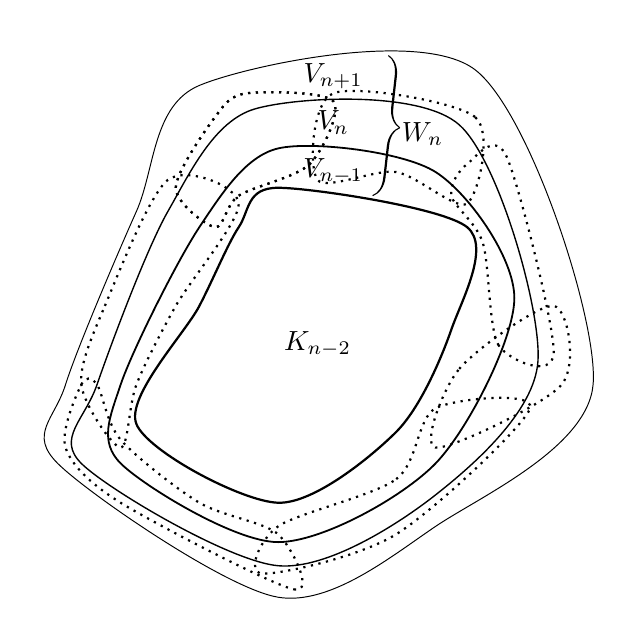
\begin{tikzpicture}
            \draw[line width=0.35] plot[smooth cycle] coordinates {
                (-0.8,1) (2,-0.7) (4,0.2) (6,2) (4.5,6) (1,5.8) (0.2,4.2) (-0.7,2)
            };
            \draw[line width=0.5] plot[smooth cycle] coordinates {
                (-0.5,1) (2,-0.3) (4,0.6) (5.3,2.3) (4.3,5.3) (1.7,5.5) (0.6,4.2) (-0.3,2)
            };
            \draw[line width=0.65] plot[smooth cycle] coordinates {
                (0,1) (2,0) (4,1) (5,3.1) (4,4.7) (2,5) (1,4) (0,2)
            };
            \draw[thick] plot[smooth cycle] coordinates {
                (0.2,1.5) (2,0.5) (3.5,1.4) (4.2,2.7) (4.4,4) (2,4.5) (1.5,4) (1,3)
            };
            \draw[thick, dotted] plot[smooth cycle] coordinates {
                (4.4,4.3) (4.5,5.4) (2.7,5.7) (2.5,4.6) (3.5,4.7)
            };
            \draw[thick, dotted] plot[smooth cycle] coordinates {
                (1.2,4) (0.7,4.5) (1.2,5.4) (1.6,5.7) (2.7,5.6) (2.4,4.8) (1.5,4.4)
            };
            \draw[thick, dotted] plot[smooth cycle] coordinates {
                (1.2,4) (0.7,4.5) (1.2,5.4) (1.6,5.7) (2.7,5.6) (2.4,4.8) (1.5,4.4)
            };
            \draw[thick, dotted] plot[smooth cycle] coordinates {
                (-0.5,2) (-0.2,3) (0.6,4.6) (1.5,4.3) (0.7,3) (0.2,2) (0,1.2)
            };
            \draw[thick, dotted] plot[smooth cycle] coordinates {
                (0,0.5) (2.2,-0.6) (2,0.1) (1,0.5) (0,1.3) (-0.3,2) (-0.5,2) (-0.7,1.2)
            };
            \draw[thick, dotted] plot[smooth cycle] coordinates {
                (2,0.2) (3.5,0.8) (4,1.7) (5.2,1.7) (3.5,0.1) (1.8,-0.4)
            };
            \draw[thick, dotted] plot[smooth cycle] coordinates {
                (4,1.2) (4.3,2.2) (5.5,3) (5.6,2)
            };
            \draw[thick, dotted] plot[smooth cycle] coordinates {
                (5.5,2.4) (4.8,2.5) (4.6,3.8) (4.2,4.4) (4.4,4.8) (4.9,4.9)
            };

            \node[anchor=north] at (2.5,2.8) {\(K_{n-2}\)};
            \node[anchor=north] at (2.7,5) {\(V_{n-1}\)};
            \node[anchor=north] at (2.7,5.6) {\(V_n\)};
            \node[anchor=north] at (2.7,6.2) {\(V_{n+1}\)};
            \draw[decorate,decoration={calligraphic
            brace, amplitude=7pt},thick] (3.4,6.18) -- (3.2,4.4) node[midway, yshift=-3pt,right=4pt] {\(W_n\)};
        \end{tikzpicture}
        \caption{The geometry of the finite subcover of \(V_n\subset W_n\) for some \(n\in\mathbb{N}\).}
        \label{fig:locallyfiniteopencoverexistence}
    \end{figure}Let \(K_{-1}=K_0=\emptyset,K_1,K_2,\cdots\subset\Omega\) exhaust \(\Omega\), with each \(K_n\) compact and \(K_n\subseteq \interior{K_{n+1}}\). For each \(n\in\mathbb{N}\), define \(W_n=\interior{K_{n+1}}\setminus K_{n-2}\), which is open, and \(V_n=K_n\setminus \interior{K_{n-1}}\), which is compact (as in \cref{fig:locallyfiniteopencoverexistence}).

    By construction, \(V_n\subseteq W_n\) for all \(n\in\mathbb{N}\). The sets \(\{V_n\}\) form compact shells exhausting \(\Omega\), since \(\bigcup_{n\in\mathbb{N}}V_n=\Omega\).

    \(\forall n\in\mathbb{N}\) and \(\forall z\in V_n\), since \(W_n\) is an open set containing \(z\) and \(\mathfrak{B}\) is a basis, there exists \(U_{z,n}\in\mathfrak{B}\) such that \(z\in U_{z,n}\subseteq W_n\) (in short, \(U_{z,n}\) is an open neighborhood of \(z\) that is contained in \(W_n\)). The collection \(\cbraces{U_{z,n}}{z\in V_n}\) is an open cover of the compact set \(V_n\), so by the Heine-Borel Theorem (\cref{thm:heineborel}) it admits a finite subcover of \(V_n\), as pictured in the dotted lines of \cref{fig:locallyfiniteopencoverexistence}. That is, there exist finitely many points \(z_{n,1},\ldots,z_{n,k_n}\) such that \(V_n\subset\bigcup_{i=1}^{k_n}U_{z_{n,i},n}\subseteq W_n\).

    Let \(\{U_j\}\) be the collection formed by enumerating all such \(U_{z_{n,i},n}\) for \(n\in\mathbb{N}\) and \(i=1,\ldots,k_n\). Then \(\{U_j\}\subset\mathfrak{B}\) is a countable collection whose union covers \(\Omega\), proving~\ref{itm:locallyfiniteopencoverexistence_cover}.

    For \ref{itm:locallyfiniteopencoverexistence_localfiniteness}, let \(K\subset\Omega\) be compact. Then \(\exists N\in\mathbb{N}\) such that \(K\subset \interior{K_N}\), and hence \(K\) is disjoint from \(V_n\) for all \(n>N+1\). Since each \(V_n\) intersects only finitely many \(U_j\), it follows that \(K\) intersects only finitely many of the \(U_j\). Thus, the collection is \textscsl{locally finite}.
\end{proof}
\begin{remark}
    The property of local finiteness of an open collection \(S\) in \(\Omega\) is commonly stated as:
    \begin{quote}
        \(\forall z\in\Omega\), there exists an open neighborhood of \(z\) intersecting finitely many sets in \(S\).
    \end{quote}
    Obviously, this assertion implies \ref{itm:locallyfiniteopencoverexistence_localfiniteness} in \cref{lem:locallyfiniteopencoverexistence}: let \(K\subset \Omega\) be compact, and for every \(z\in\Omega\), the collection of neighborhoods covers \(K\), and by the Heine--Borel Theorem (\cref{thm:heineborel}), admits a finite subcover. Therefore, \(K\) intersects finitely many sets in \(S\). Conversely, \(\forall z\in\Omega\), there exists an open neighborhood \(V\ni z\) relatively compact in \(\Omega\). By assumption, \(\overline{V}\) intersects finitely many sets in \(S\), and since \(V\subset\overline{V}\), the conclusion follows.
\end{remark}
\begin{theorem}[\textsc{Partition of Unity}]\label{thm:partitionofunity}
    For a nonempty open set \(\Omega\subseteq\mathbb{C}\), suppose that \(\cbraces{\Omega_k}_{k\in\mathbb{Z}_{\ge0}}\) is an open cover of \(\Omega\). Then, there exists a collection of bump functions \(\alpha_1(z),\alpha_2(z),\ldots\in C^\infty(\mathbb{C})\), each with compact support in \(\Omega\) satisfying
    \begin{enumerate}
        \item \(\forall j\in\mathbb{N}\), \(\exists k\in\mathbb{Z}_{\geq0}\) such that \(\supp\paren{\alpha_j}\subseteq\Omega_k\).\label{itm:partitionofunity_subordinate}
        \item The collection \(\qty{\supp\paren{\alpha_j}}\) is locally finite.\label{itm:partitionofunity_localfiniteness}
        \item \(\forall j\in\mathbb{N}\), \(0\leq\alpha_j\leq 1\).\label{itm:partitionofunity_nonnegativity}
        \item \(\forall z\in\Omega\), \(\sum_{j=1}^\infty \alpha_j(z)=1,\)\label{itm:itm:partitionofunity_partitionofunity}
    \end{enumerate} known as a \(C^\infty\) partition of unity \textscsl{subordinate to} \(\cbraces{\Omega_k}_{k\in\mathbb{Z}_{\geq0}}\).
\end{theorem}
\begin{proof}
    By the openness of \(\Omega_k\), \(\forall z\in\Omega\), \(\exists r_z>0\) such that \(\overline{D\paren{z,r_z}}\subset\Omega_{k_z}\) for some \(k_z\in\mathbb{Z}_{\ge0}\).

    Then, \(\cbraces{D\paren{z,r}}{z\in\Omega, 0<r<r_z}\) forms an open basis of \(\Omega\). By \cref{lem:locallyfiniteopencoverexistence}, there exists a locally finite open cover \(\cbraces{D\paren{z_j,r_{z_j}}}\) of \(\Omega\), and since it is a subcollection of the basis, \[D\paren{z_j,r_{z_j}}\subset\overline{D\paren{z_j,r_{z_j}}}\subset\Omega_{k_{z_j}},\quad\forall j\in\mathbb{N}.\] The most trivial bump function has the form \[\theta(z)=
        \begin{cases}
            \exp\paren{\frac{1}{\abs{z}^2-1}} &\qif* \abs{z}<1   \\
            0                                 &\qif* \abs{z}\ge1
    \end{cases},\] which has the support \(\overline{D(0,1)}\). Define the function \(\theta_\varepsilon(z)=\varepsilon^{-2}\theta\qty(\frac{z}{\varepsilon})\) with the support \(\overline{D(0,\varepsilon)}\), which satisfies that \(\forall\varepsilon>0\), \[\int_{\mathbb{C}}\theta_\varepsilon(z)\ddx\wedge\ddy=1.\]
    Define a set of functions \(\cbraces{\beta_j(z)}_{j\in\mathbb{N}}\) with \(\beta_j(z)=\theta_{r_{z_j}}\paren{z-z_j}\), which is a bump function with \(\supp\qty(\beta_j)=\overline{D\paren{z_j, r_{z_j}}}\subset\Omega_{k_{z_j}}\).

    By the local finiteness of \(\qty{D\qty(z_j,r_{z_j})}\), there exists an open neighborhood \(V_z\) of each point \(z\in\Omega\) such that the set \(\cbraces{j}{V_z\cap D\qty(z_j,r_{z_j})\neq\emptyset}\) is finite. Since every open neighborhood of each point in \(\overline{D\qty(z_j,r_{z_j})}\) intersects \(D\qty(z_j,r_{z_j})\), it follows that every open set disjoint from \(D\qty(z_j,r_{z_j})\) is also disjoint from its closure. Since \(\overline{D\qty(z_j,r_{z_j})}\supset D\qty(z_j,r_{z_j})\), any open set intersecting \(D\qty(z_j,r_{z_j})\) will intersect \(\overline{D\qty(z_j,r_{z_j})}\). Therefore, \(\cbraces{j}{V_z\cap\overline{D\qty(z_j,r_{z_j})}\neq\emptyset}\) is finite. Equivalently, \(\cbraces{\supp\paren{\beta_j}}_{j\in\mathbb{N}}\) is locally finite on \(\Omega\).

    Consequently, \(\forall z_0\in\Omega\), there exists an open neighborhood \(V\ni z_0\) that intersects a finite number of sets in \(\cbraces{\supp\paren{\beta_j}}_{j\in\mathbb{N}}\). Then \(\forall z\in V\), the sum \[S(z)=\sum_{j=1}^\infty\beta_j(z)\] is a sum of finitely many terms and is therefore \(C^\infty\) at \(z_0\). Since the collection of supports exhausts \(\Omega\), \(S(z)\) is positive. Therefore, the sequence defined by \[\alpha_j(z)={\frac{\beta_j(z)}{S(z)}}\] is also \(C^\infty\) and is compactly supported in \(\Omega\). Furthermore, we have \[\sum_{j=1}^\infty\alpha_j(z)=1,\] as desired.
\end{proof}
\begin{theorem}[Existence of Bump Functions]\label{thm:bumpfunctionexistence}
    Let \(\Omega\subset\mathbb{C}\) be open, \(K\subset\Omega\) be compact, and \(V\subseteq\Omega\) be an open neighborhood of \(K\). Then there exists a bump function \(\varphi\in C^\infty\paren{\mathbb{C}}\) with compact support contained in \(V\) such that \(\forall z\in\mathbb{C}\), \(0\leq\varphi(z)\leq 1\), and there exists an open neighborhood of \(K\) over which \(\varphi\equiv1\).
\end{theorem}
\begin{proof}
    Let \(V(K,\varepsilon)=\cbraces{z\in\mathbb{C}}{\inf_{\zeta\in K}\abs{\zeta-z}<\varepsilon}\), an \(\varepsilon\)-neighborhood of \(K\).

    Then \(\exists\varepsilon>0\) such that \(K\subset V(K,\varepsilon)\subset V(K,2\varepsilon)\subseteq V\). Let \(\Omega_1=V(K,2\varepsilon)\) and \(\Omega_2=\Omega\setminus V(K,\varepsilon)\). Then there exists a \(C^\infty\) partition of unity \(\cbraces{\alpha_j(z)}_{j\in\mathbb{N}}\) of \(\Omega\) subordinate to the open cover \(\cbraces{\Omega_1,\Omega_2}\). Define a new function
    \[\varphi(z)=\sum_{\substack{j\in\mathbb{N}\\\supp{\alpha_j}\subseteq\Omega_1}}\alpha_j(z).\]
    It follows that \(\varphi\in C^\infty(\mathbb{C})\) with compact support in \(\Omega_1\). Since the support of every \(\alpha_j\) where \(j\in\mathbb{N}\) lies entirely either in \(\Omega_1\) or \(\Omega_2\), \[1=\sum_{\substack{j\in\mathbb{N}\\\supp{\alpha_j}\subseteq\Omega_2}}\alpha_j(z)+\varphi(z).\]
    When \(z\in\Omega_1\setminus\Omega_2=V(K,\varepsilon)\), the first summation vanishes, meaning that \(\varphi(z)\equiv1\) on the neighborhood \(V(K,\varepsilon)\) of \(K\). When \(z\in\Omega_2\setminus\Omega_1=\Omega\setminus V(K,2\varepsilon)\), \(\varphi(z)\) vanishes.
\end{proof}
\subsection{Zeros of a Holomorphic Function}
For a region \(U\subseteq\mathbb{C}\) and a holomorphic function \(f:U\to\mathbb{C}\), a point \(z_0\in U\) is a \textscsl{zero} of \(f\) iff \(f\paren{z_0}=0\). Furthermore, if \(f\) has the Taylor expansion at \(z_0\) of \[a_m\paren{z-z_0}^m+a_{m+1}\paren{z-z_0}^{m+1}+\cdots,\qquad m\in\mathbb{N},a_m\neq0,\] then the zero at \(z_0\) has multiplicity \(m\).

We will introduce a fundamental application of Liouville's Theorem (\cref{thm:liouville}) below.
\begin{theorem}[Fundamental Theorem of Algebra]\label{thm:fundamentaltheoremofalgebra}
    Every non-constant polynomial \(p(z)\) with complex coefficients has at least one complex zero.
\end{theorem}
\begin{proof}
    For the sake of contradiction, suppose that \(p(z)\) has no complex zeros. Then the function \(f(z)=\frac{1}{p(z)}\) is continuous and entire, because \(p(z)\) has no zeros in \(\mathbb{C}\). Moreover, as \(z\to\infty\), \(p(z)\to\infty\), so \(f(z)\to 0\), and thus \(f(z)\) is bounded. By Liouville's Theorem (\cref{thm:liouville}), every bounded entire function is constant. Thus, \(f(z)\) is constant, and so \(p(z)\) must also be constant. By contradiction, \(p(z)\) has at least one complex zero.
\end{proof}
\begin{theorem}\label{thm:identityaccumulationofzeros}
    Let \(U\subseteq\mathbb{C}\) be open and connected, and \(f:U\to\mathbb{C}\) be holomorphic over \(U\). Then if the set defined by \(S=\cbraces{z\in U}{f(z)=0}\) has an accumulation point in \(U\), then \(f\equiv0\) over \(U\).
\end{theorem}
\begin{proof}
    Let \(\cbraces{z_n}_{n\in\mathbb{N}}\) be a subset of \(S\) and assume it has an accumulation point \(z_\infty\) in \(U\). Since \(f\) is holomorphic over \(U\), \(\exists\varepsilon>0\) such that \(f\) is holomorphic over \(D\paren{z_\infty,\varepsilon}\subseteq U\). Then over this disk, \(f\) has the Taylor expansion
    \begin{equation}\label{eq:identityaccumulationofzeros_taylorexpansion}
        f(z)=\sum_{n=0}^\infty a_n\paren{z-z_\infty}^n.
    \end{equation}
    By \cref{def:accumulationpoint}, \(\exists N\in\mathbb{N}\) such that \(\forall n>N\), \(z_n\in D\paren{z_\infty,\varepsilon}\). Since \(z_n\) is a zero of \(f\), \(f\paren{z_n}=0\). Then, by the continuity of \(f\), \[\lim_{n\to\infty} f\paren{z_n}=f\paren{\lim_{n\to\infty}z_n}=f\paren{z_\infty}=0.\] Using this result in comparison to \cref{eq:identityaccumulationofzeros_taylorexpansion}, we get that \(a_0=0\).

    The function \(f_1(z)=\frac{f(z)}{z-z_\infty}\) has a Taylor expansion over \(D\paren{z_0,\varepsilon}\) of
    \[f_1(z)=\sum_{n=0}^\infty a_{n+1}\paren{z-z_\infty}^n.\]
    Let \(z=z_n\neq z_\infty\) for some \(n>N\). Then \(f_1\) vanishes, leaving \[0=a_1+\order{z_n-z_\infty}.\]
    Letting \(n\to\infty\), \(z_n\to z_\infty\), and \(a_1=0\). Define \(f_2(z)=\frac{f_1(z)}{z-z_\infty}\). Then, \[f_2(z)=\sum_{n=0}^\infty a_{n+2}\paren{z-z_\infty}^n.\]
    Similarly, \(a_2=0\). Letting \(f_n(z)=\frac{f(z)}{\paren{z-z_\infty}^n}\), the sequence \(\cbraces{a_n}_{n\in\mathbb{Z}_{\geq0}}\) vanishes, and \(f\equiv 0\) on \(D\paren{z_\infty,\varepsilon}\).

    Let \(\widetilde{S}=\cbraces{z\in U}{\forall n\in\mathbb{Z}_{\geq0}, f^{(n)}(z)=0}\).\ \(\forall z\in D\paren{z_\infty,\varepsilon}\), since \(f(z)\) locally vanishes (and has vanishing derivatives as a consequence), \(D\paren{z_\infty,\varepsilon}\subseteq \widetilde{S}\). Furthermore, \(\forall z'\in \widetilde{S}\), \(\exists\varepsilon'>0\) such that \(f(z)\) has a convergent Taylor series with vanishing coefficients on \(D(z',\varepsilon')\subseteq U\). Then \(f\equiv0\) on \(D\paren{z',\varepsilon'}\). Then \(\forall z\in D(z',\varepsilon')\), since \(f\) is constant at \(z\), it also has vanishing derivatives. It follows that \(D(z',\varepsilon')\subseteq \widetilde{S}\). Since every point in \(\widetilde{S}\) has an open neighborhood also in \(\widetilde{S}\), \(\widetilde{S}\) is open.

    It is evident that \(\forall k\in\mathbb{Z}_{\geq0}\), \(f^{(k)}\) is continuous in \(U\) by the holomorphy of \(f\). Let \(S_k=\cbraces{z\in U}{f^{(k)}(z)=0}\). For any sequence \(\cbraces{\widetilde{z}_n}\in S_k\) converging to some \(\widetilde{z}_\infty\in U\), by the continuity of \(f\), \[\lim_{n\to\infty} f^{(k)}\paren{\widetilde{z}_n}=f^{(k)}\paren{\lim_{n\to\infty}\widetilde{z}_n}=f^{(k)}\paren{z'_\infty}=0,\] and therefore \(\widetilde{z}_\infty\in S_k\). Thus, \(S_k\) contains all of its accumulation points in \(U\) and is therefore closed in \(U\) (if \(\widetilde{z}_\infty\notin U\), then it is no longer relevant; we are concerned about it being closed within \(U\)). Since \(\widetilde{S}=\bigcap_{k\in\mathbb{Z}_{\geq0}} S_k\) and each of \(S_k\) is closed in \(U\), \(\widetilde{S}\) is the intersection of closed sets and consequently closed.

    Since \(\widetilde{S}\) is nonempty and clopen in the connected set \(U\), \(\widetilde{S}=U\) (by \cref{thm:connectedtopologicalspaceclopensets}). It follows that \(f\equiv 0\) on \(U\).
\end{proof}
\begin{remark}
    This is a trivial property of holomorphic functions that allows for the uniqueness of analytic continuations. It is oftentimes stated in the form below:
\end{remark}
\begin{theorem}[Identity Theorem]\label{thm:identity}
    Let \(U\subseteq\mathbb{C}\) be open and connected, and define \(f(z)\) and \(g(z)\) to be two holomorphic functions on \(U\). For a set \(S\subseteq U\) with an accumulation point in \(U\), if \(f\equiv g\) on \(S\), then \(f\equiv g\) on \(U\).
\end{theorem}
\begin{proof}
    Let \(h=f-g\) be holomorphic over \(U\). Since \(S\) has an accumulation point in \(U\), and \(h\equiv 0\) over \(S\), then by \cref{thm:identityaccumulationofzeros}, \(h\equiv 0\) over \(U\).
\end{proof}
\begin{theorem}[Holomorphic Argument Principle]\label{thm:argumentprincipleholomorphic}
    Let \(U\subseteq\mathbb{C}\) be a region and \(f:U\to\mathbb{C}\) be holomorphic. Let \(\gamma\subset U\) be a simple, closed, positively oriented curve that is null-homotopic in \(U\). If \(f\) has no zeros on \(\gamma\), then \(f\) has finitely many zeros in the region bounded by \(\gamma\), and this number, counting multiplicities, is given by
    \[k=\frac{1}{2\piup\ii}\oint_{\gamma}\frac{f'(z)}{f(z)}\ddz.\]
    Let \(\Gamma\) be the image of \(\gamma\) under the map \(w=f(z)\). Then \(k=\frac{1}{2\piup}\Delta_\Gamma\arg(w)\), where \(\Delta_\Gamma\arg(w)\) denotes the total change in argument of \(w\) as it traverses \(\Gamma\).
\end{theorem}
\begin{proof}
    Let \(z_1,\ldots,z_n\) be the distinct zeros of \(f\) enclosed by \(\gamma\) with the respective multiplicities \(k_1,\ldots,k_n\). Choose disjoint disks \(D\qty(z_j,\varepsilon_j)\) centered at each \(z_j\) with radii \(\varepsilon_j>0\), each contained in the interior of \(\gamma\) and avoiding \(\gamma\). The function \[\frac{f'(z)}{f(z)}\]
    is holomorphic on the domain \[\mathrm{int}\paren{\gamma}\setminus\bigcup_{j=1}^n \overline{D\qty(z_j,\varepsilon_j)},\]
    where \(\mathrm{int}(\gamma)\) denotes the interior relative to \(\gamma\). The oriented boundary of this domain is \(\gamma^+\cup\bigcup_{j=1}^n\partial D\paren{z_j,\varepsilon_j}^-\). By Cauchy--Goursat (\cref{thm:cauchygoursattheorem}),
    \[\int_{\gamma^+\cup\bigcup_{j=1}^n\partial D\paren{z_j,\varepsilon_j}^-}\frac{f'(z)}{f(z)}\ddz=0,\]
    which rearranges to
    \[\oint_{\gamma^+}\frac{f'(z)}{f(z)}\ddz=\sum_{j=1}^n\oint_{\partial D\paren{z_j,\varepsilon_j}^+}\frac{f'(z)}{f(z)}\ddz.\]
    Near each \(z_j\), express \(f(z)=\paren{z-z_j}^{k_j}h_j(z)\) where \(h_j\) is holomorphic and non-vanishing on \(D\paren{z_j,\varepsilon_j}\). Differentiation yields
    \[f'(z)=k_j\paren{z-z_j}^{k_j-1}h_j(z)+\paren{z-z_j}^{k_j}h_j'(z),\] and thus
    \[\frac{f'(z)}{f(z)}=\frac{k_j}{z-z_j}+\frac{h_j'(z)}{h_j(z)}.\]
    Since \(h_j\) is holomorphic and non-vanishing on \(D\paren{z_j,\varepsilon_j}\), the function \(\frac{h_j'}{h_j}\) is holomorphic there. By the Cauchy--Goursat Theorem,
    \[\oint_{\partial D\paren{z_j,\varepsilon_j}}\frac{h_j'(z)}{h_j(z)}\ddz=0.\]
    The Cauchy--Goursat Formula (\cref{thm:cauchygoursatformula}) gives
    \[\oint_{\partial D\paren{z_j,\varepsilon_j}}\frac{k_j}{z-z_j}\ddz=2\piup \ii k_j.\]
    Combining results,
    \[\oint_{\gamma}\frac{f'(z)}{f(z)}\ddz=\sum_{j=1}^n2\piup \ii k_j=2\piup \ii k.\]
    Finally, parameterize \(\Gamma\) by \(w=f(z)\). Then \(\dd{w}=f'(z)\ddz\), and
    \[k=\frac{1}{2\piup\ii}\oint_{\Gamma}\frac{\dd{w}}{w}=\frac{1}{2\piup\ii}\Delta_\Gamma\log(w)=\frac{1}{2\piup}\Delta_\Gamma\arg(w),\] which proves the result.
\end{proof}
Thus, one defines the \textscsl{winding index} to quantify how many times a closed curve winds counterclockwise around a given point in the complex plane. Formally, if \(\gamma=\gamma([0,1])\) is a counterclockwise-oriented closed curve and \(z\) is a point satisfying \(z\notin\gamma\), then \[\mathrm{Ind}_{\gamma}(z)=\frac{1}{2\piup\ii}\int_\gamma\frac{\ddzeta}{\zeta-z}=\frac{1}{2\piup\ii}\int_0^1\frac{\gamma'(t)\ddt}{\gamma(t)-z}.\]
\begin{theorem}\label{thm:hurwitzsimplecase}
    Let \(\cbraces{f_n(z)}\) be a sequence of holomorphic functions on the open set \(U\subseteq\mathbb{C}\) that uniformly converges to \(f(z)\) on every compact subset of \(U\). If \(\forall n\in\mathbb{N}\), \(f_n(z)\) has no zeros in \(U\), then \(f\) is either identically 0 or has no zeros in \(U\).
\end{theorem}
\begin{proof}
    By the holomorphy of \(f_n(z)\), for any simple closed rectifiable curve \(\gamma\subset U\) (whose interior is a subset of \(U\)), by the Cauchy--Goursat Theorem (\cref{thm:cauchygoursattheorem}), \[\oint_{\gamma}f_n(\zeta)\ddzeta=0.\] Since \(\gamma\) is a subset of any compact subset of \(U\), \(\cbraces{f_n(\zeta)}\) uniformly converges on \(\gamma\), and by \cref{thm:limitintegralswitch},
    \begin{equation}
        \lim_{n\to\infty}\oint_{\gamma}f_n(\zeta)\ddzeta=\oint_{\gamma}\lim_{n\to\infty}f_n(\zeta)\ddzeta=\oint_{\gamma}f(\zeta)\ddzeta=0.\label{eq:hurwitzsimplecase_integrallimitswitchforholomorphy}
    \end{equation}
    Then by Morera's Theorem (\cref{thm:morera}), \(f(z)\) is holomorphic, and \(f'(z)\) is holomorphic. We aim to show that \(f'_n(z)\rightrightarrows f'(z)\).

    Let \(K\subset U\) be arbitrary and compact and \(V\supset K\) be open and relatively compact in \(U\). Since \(\cbraces{f'_n(z)}\) is holomorphic, by \cref{cor:nthderivativeboundedsupremum}, there exists a finite constant \(c>0\) such that \[\lim_{n\to\infty}\sup_{z\in K}\abs{f'_n(z)-f'(z)}\leq c\lim_{n\to\infty}\sup_{z\in V}\abs{f_n(z)-f(z)}.\]

    By the definition of uniform convergence, the right-hand side approaches 0, and \(\cbraces{f'_n(z)}\) is then uniformly convergent to \(f'(z)\) by the same reasoning.

    Through the proof of \cref{thm:identityaccumulationofzeros}, if \(f\not\equiv0\) over \(U\), then the zeros of \(f\) do not have an accumulation point in \(U\) and are therefore discrete. In this case, let \(\gamma\subset U\) be a curve that does not pass through the zeros of \(f\). Since each function in the sequence \(f_n\) does not contain zeros in \(U\), by the Argument Principle, (\cref{thm:argumentprincipleholomorphic}),
    \begin{equation}
        \lim_{n\to\infty}\oint_{\gamma}\frac{f_n'(z)}{f_n(z)}\ddz=0.\label{eq:hurwitzsimplecase_argumentprinciple}
    \end{equation}
    Since \(f\) and \(f'\) are holomorphic over \(\gamma\), by \cref{thm:continuousfunctionboundedoncompact}, there exists a finite value \(M>0\) such that \(\forall z\in\gamma\), \(\max\qty{\abs{f(z)},\abs{f'(z)}}<M\).

    Since \(\gamma\) does not pass through the zeros of \(f\), \(\exists\lambda>0\) such that \(\forall z\in\gamma\), \(\abs{f(z)}>\lambda\). By the uniform convergence of \(\cbraces{f_n(z)}\), \(\exists N\in\mathbb{N}\) such that
    \[\abs{f_n(z)-f(z)}<\frac{\lambda}{2},\quad\forall n>N,\forall z\in\gamma.\]
    Then \(\abs{f_n(z)}>\frac{\lambda}{2}\) on \(\gamma\). Hence, \(\frac{1}{f_n(z)}\) and its limit are uniformly bounded; \[\abs{\frac{1}{f(z)}}<\frac{1}{\lambda},\quad\abs{\frac{1}{f_n(z)}}<\frac{2}{\lambda},\quad\forall z\in\gamma,\forall n>N.\]
    Then,
    \begin{align*}
        \abs{\frac{f'}{f}-\frac{f'_n}{f_n}}                                               & =\abs{\frac{f'f_n-f'_n f}{f_n f}}                                                                         \\
        & <2\frac{\abs{f'f_n-f'f}+\abs{f'f-f'_n f}}{\lambda^2}                                                     \\
        & <\frac{2M}{\lambda^2}\cdot\paren{\abs{f_n-f}+\abs{f'-f'_n}}.                                            \\
        \sup_{z\in\gamma}\abs{\frac{f'(z)}{f(z)}-\frac{f'_n(z)}{f_n(z)}}                  & \leq\frac{2M}{\lambda^2}\paren{\sup_{z\in\gamma}\abs{f_n(z)-f(z)}+\sup_{z\in\gamma}\abs{f'(z)-f'_n(z)}} \\
        \lim_{n\to\infty}\sup_{z\in\gamma}\abs{\frac{f'(z)}{f(z)}-\frac{f'_n(z)}{f_n(z)}} & \leq\frac{2M}{\lambda^2}\paren{\lim_{n\to\infty}\sup_{z\in\gamma}\abs{f_n(z)-f(z)}+\abs{f'(z)-f'_n(z)}} \\
        & =0.
    \end{align*}
    Therefore, \(\frac{f'(z)}{f(z)}\) is uniformly convergent on \(\gamma\). By \cref{thm:limitintegralswitch}, we can pass the limit through the integral in \cref{eq:hurwitzsimplecase_argumentprinciple}. Then,
    \[\lim_{n\to\infty}\oint_\gamma \frac{f'_n(z)}{f_n(z)}\ddz=\oint_\gamma \frac{f'(z)}{f(z)}\ddz=0.\] By the Argument Principle, (\cref{thm:argumentprincipleholomorphic}), \(f(z)\) has no zeros in the interior of \(\gamma\). Since \(\gamma\) was arbitrarily chosen, either \(f(z)\equiv 0\) on \(U\) or has no zeros in \(U\).
\end{proof}
\begin{theorem}[\textsc{Rouché}]\label{thm:rouche}
    Let \(U\subseteq\mathbb{C}\) be open and \(f,g\) be two holomorphic functions over \(U\). Let \(\gamma\subset U\) be a simple, closed, rectifiable curve, and \(\forall z\in\gamma\)
    \begin{equation}
        \abs{f(z)-g(z)}<\abs{f(z)}\label{eq:rouche}.
    \end{equation} Then \(f\) and \(g\) have the same number of zeros enclosed by \(\gamma\) and do not vanish on \(\gamma\).
\end{theorem}
\begin{proof}
    It is obvious that \(g(z)\) has no zeros on \(\gamma\). Otherwise, \(\exists z_0\in\gamma\) such that \(g\paren{z_0}=0\), implying that \(\abs{f\paren{z_0}}<\abs{f\paren{z_0}}\) which is impossible. Similarly, \(f(z)\) has no zeros on \(\gamma\), since \(\abs{g(z)}<0\) is an impossibility.

    Let \(k_f\) and \(k_g\) denote the number of zeros of \(f\) and \(g\) enclosed by \(\gamma\), respectively. By the Argument Principle (\cref{thm:argumentprincipleholomorphic}),
    \begin{align*}
        k_g-k_f & =\int_{\gamma}\frac{g'(z)}{g(z)}\ddz-\int_\gamma\frac{f'(z)}{f(z)}\ddz                                                    \\
        & =\int_\gamma\frac{g'(z)f(z)-f'(z)g(z)}{g(z)f(z)}\ddz=\int_\gamma\frac{\qty(\frac{g(z)}{f(z)})'}{\frac{g(z)}{f(z)}}\ddz.
    \end{align*}
    Let \(w=h(z)=\frac{g(z)}{f(z)}\) with \(\Gamma=h(\gamma)\). Then, \[k_g-k_f=\int_\Gamma\frac{\dd{w}}{w}.\]
    From \cref{eq:rouche}, by dividing both sides by \(f(z)\), we obtain \(\abs{w-1}<1\). Then \(\Gamma\) lies in the open disk \(D(1,1)\), which will never intersect or enclose 0. Then by \cref{lem:cauchyintegraltheoremoversimplyconnectedset}, \[k_g-k_f=\int_\Gamma\frac{\dd{w}}{w}=0,\] as desired.
\end{proof}
By the Fundamental Theorem of Algebra (\cref{thm:fundamentaltheoremofalgebra}), any polynomial in the form \(p(z)=\sum_{k=0}^n a_kz^k\) (\(n\in\mathbb{N}\), \(a_n\neq 0\), \(a_k\in\mathbb{C}\) where \(k=1,\ldots n\)) has at least one complex zero. Consider the function \(q(z)=a_nz^n\), with a zero at \(z=0\) with multiplicity \(n\). By Rouché's Theorem (\cref{thm:rouche}), since \(\exists R\in\mathbb{R}\) such that \(\abs{q(z)-p(z)}=\abs{\sum_{k=0}^{n-1}a_k z^k}<\abs{a_n z^n}\) over \(\abs{z}=R\), \(p\) and \(q\) have the same number of zeros, counting multiplicity.
\begin{theorem}\label{thm:hurwitzshifts}
    Let \(U\subseteq\mathbb{C}\) be open and connected, and \(f(z)\) be holomorphic and non-constant on \(U\).

    If \(z_0\in U\) and \(w_0=f\qty(z_0)\), and the multiplicity of the zero at \(z_0\) of \(f-w_0\) is \(m\), then for all \(\rho>0\) such that \(f-w_0\) is non-vanishing on \(\overline{D\qty(z_0,\rho)}\setminus\qty{z_0}\), \(\exists\delta>0\) such that \(\forall\xi\in D\qty(w_0,\delta)\), \(f-\xi\) has \(m\) zeros in \(D\qty(z_0,\rho)\), counting multiplicity.
\end{theorem}
\begin{proof}
    The zero at \(z_0\) is isolated by \cref{thm:identityaccumulationofzeros}. Furthermore, \(\abs{f-w_0}\) is continuous on \(\partial D\qty(z_0,\rho)\) and attains a positive infimum \(\delta\). In other words, on this set, \(\abs{f-w_0}\geq\delta\). Hence, \(\forall \xi\in D\qty(w_0,\delta)\), we have \(\abs{\xi-w_0}<\delta\leq\abs{f(z)-w_0}\) for any \(z\in\partial D\qty(z_0,\rho)\).

    By Rouché's Theorem, since \(\abs{\qty(f(z)-w_0)-\qty(f(z)-\xi)}<\abs{f(z)-w_0}\), it follows that \(f-\xi\) and \(f-w_0\) have the same number of zeros in \(D\qty(z_0,\rho)\).
\end{proof}
We also have the following generalization of \cref{thm:hurwitzsimplecase}, which is a heuristic restatement of \cref{thm:hurwitzshifts}:
\begin{theorem}[\textsc{Hurwitz}]\label{thm:hurwitz}
    Let \(U\subseteq\mathbb{C}\) be an open and connected set, and suppose \(\qty{f_n(z)}_{n\in\mathbb{N}}\) is a holomorphic function sequence that uniformly converges to a non-constant function \(f(z)\) on all compact sets of \(U\).

    If \(z_0\in U\) and \(w_0=f\qty(z_0)\), and the multiplicity of the zero at \(z_0\) of \(f-w_0\) is \(m\), then for all \(\rho>0\) such that \(f-w_0\) is non-vanishing on \(\overline{D\qty(z_0,\rho)}\setminus\qty{z_0}\), \(\exists N\in\mathbb{N}\) such that \(\forall n>N\), \(f_n-w_0\) has \(m\) zeros in \(D\qty(z_0,\rho)\), counting multiplicity.
\end{theorem}
\begin{proof}
    The zero at \(z_0\) is isolated by \cref{thm:identityaccumulationofzeros}. Furthermore, \(\abs{f-w_0}\) is continuous on \(\partial D\qty(z_0,\rho)\) and attains a positive infimum \(\delta\). In other words, on this set, \(\abs{f-w_0}\geq\delta\). By uniform convergence, \(\exists N\in \mathbb{N}\) such that \(\forall n>N\), we have \(\abs{f(z)-f_n\qty(z)}<\delta\leq\abs{f(z)-w_0}\) for any \(z\in\partial D\qty(z_0,\rho)\).

    By Rouché's Theorem (\cref{thm:rouche}), since \[\abs{\qty(f(z)-w_0)-\qty(f_n(z)-w_0)}<\abs{f(z)-w_0},\] it follows that \(f_n-w_0\) and \(f-w_0\) have the same number of zeros in \(D\qty(z_0,\rho)\).
\end{proof}
\subsection{Further Properties of Holomorphic Functions}
A useful corollary of \cref{thm:cauchygoursatformula} is the Maximum Modulus Principle.

Before the theorem, we first introduce the mean-value property of holomorphic functions.
\begin{lemma}\label{lem:holomorphicmeanvalueproperty}
    Let \(U\subseteq\mathbb{C}\) be open and simply connected, and let \(f:U\to\mathbb{C}\) be holomorphic. Then \(\forall z\in U\) and \(\forall \varepsilon>0\) such that \(\overline{D(z,\varepsilon)}\subset U\), \(f(z)\) is the average of \(f(\zeta)\) where \(\zeta\in D(z,\varepsilon)\) is uniform. In other words, \[f(z)=\frac{1}{2\piup\varepsilon}\oint_{\partial D(z,\varepsilon)}f(\zeta)\abs{\dd{\zeta}}.\]
\end{lemma}
\begin{proof}
    By the Cauchy--Goursat Formula (\cref{thm:cauchygoursatformula}), \[f(z)=\frac{1}{2\piup\ii}\oint_{\partial D(z,\varepsilon)}\frac{f(\zeta)}{\zeta-z}\ddzeta=\frac{1}{2\piup}\int_0^{2\piup}f\paren{z+\varepsilon \ee^{\ii t}}\dd{t}.\]
    Observe that
    \begin{align*}
        f(z)=\frac{1}{2\piup\varepsilon}\oint_{\partial D(z,\varepsilon)}f(\zeta)\abs{\dd{\zeta}} & =\frac{1}{2\piup\varepsilon}\int_{0}^{2\piup}f\paren{z+\varepsilon \ee^{\ii t}}\abs{\ii\varepsilon \ee^{\ii t}\dd{t}} \\
        & =\frac{1}{2\piup}\int_{0}^{2\piup}f\paren{z+\varepsilon \ee^{\ii t}}\dd{t},
    \end{align*}
    and the conclusion follows.
\end{proof}
Since the real and imaginary parts of holomorphic functions are real-valued harmonic functions, they also satisfy the mean-value property. Furthermore, if a real continuous function satisfies the mean-value property, it is harmonic (to be proved in \cref{thm:meanvaluepropertysolutionsareharmonic}). This equivalence allows for the alternative definition of harmonic functions.
\begin{theorem}[Maximum Modulus Principle]\label{thm:maximummodulus}
    Let \(f(z)\) be holomorphic on an open connected region \(U\subseteq\mathbb{C}\). If \(\exists z_0\in U\) and an open neighborhood \(V\subseteq U\) of \(z_0\) such that \(\forall z\in V\), \(\abs{f\paren{z_0}}\geq\abs{f(z)}\), then \(f\) is a constant function on \(U\).
\end{theorem}
\begin{proof}
    Assume that \(z_0\) exists. We will first prove that the set \[S=\cbraces{z}{f(z)=f\paren{z_0},z\in V}\]
    is all of \(V\). This is equivalent to proving that \(S\) is nonempty, open, and closed in \(V\).

    Since \(z_0\in S\), the first condition is satisfied (nonemptiness). For any sequence \(\cbraces{z_n}\in S\) converging to some \(z_\infty\in V\), by the continuity of \(f\), \[\lim_{n\to\infty} f\paren{z_n}=f\paren{\lim_{n\to\infty}z_n}=f\paren{z_\infty}=0,\] and \(z_\infty\in S\). Thus, \(S\) contains all of its accumulation points in \(V\) and is therefore closed (if \(z_\infty\notin V\), then it is no longer relevant; we are concerned with it being closed within \(V\)).

    Since \(S\subseteq V\) and \(V\) are both open, \(\forall z\in S\), \(\exists\lambda>0\) such that \(D(z,\lambda)\subseteq V\). By \cref{lem:holomorphicmeanvalueproperty}, \(\forall 0<\varepsilon<\lambda\),
    \begin{align*}
        |f(z)| & =\abs{\frac{1}{2\piup}\int_0^{2\piup}f\paren{z+\varepsilon \ee^{\ii t}}\dd{t}}\leq \frac{1}{2\piup}\int_0^{2\piup}\abs{f\paren{z+\varepsilon \ee^{\ii t}}}\dd{t} \\
        & \leq\frac{1}{2\piup}\int_0^{2\piup}\abs{f(z)}\dd{t}=\abs{f(z)}.
    \end{align*}
    It follows that all inequalities above are equalities, or that
    \begin{align*}
        |f(z)| & =\abs{\frac{1}{2\piup}\int_0^{2\piup}f\paren{z+\varepsilon \ee^{\ii t}}\dd{t}}=\frac{1}{2\piup}\int_0^{2\piup}\abs{f\paren{z+\varepsilon \ee^{\ii t}}}\dd{t} \\
        & =\frac{1}{2\piup}\int_0^{2\piup}\abs{f(z)}\dd{t}=\abs{f(z)}.
    \end{align*}
    From the equality of the last two integrals, \(\int_{0}^{2\piup}\qty(\abs{f(z)}-\abs{f\paren{z+\varepsilon \ee^{\ii t}}})\dd{t}=0\). Since this integrand is strictly non-negative, we have equality. Thus, \(\forall z\in S\), \(\exists\lambda>0\) such that \(D\paren{z,\lambda}\subseteq S\). In other words, every \(z\in S\) has an open neighborhood that also lies in \(S\). Therefore, \(S\) is open and \(S=V\) as it is a nonempty clopen subset. Since \(V\) is nonempty and open, it has an accumulation point in \(U\). It follows that \(f(z)\equiv f\paren{z_0}\) over \(U\) by the Identity Theorem (\cref{thm:identity}).
\end{proof}
\begin{remark}
    If \(f\) is holomorphic and non-constant on an open region \(U\subseteq\mathbb{C}\), then for any compact set \(K\subset U\), the maximum of \(f\) in \(K\) lies on \(\partial K\). Otherwise, \(f\) would attain a maximum at some \(z\in \interior{K}\), and contradict the statement of \cref{thm:maximummodulus} under the assumption of being non-constant.
\end{remark}
A similar theorem exists for real-valued harmonic functions. The proof follows in the same way as the one for holomorphic functions. We will state it formally below.
\begin{theorem}\label{thm:maximumprincipleforrealharmonicfunctions}
    Let \(U\subseteq\mathbb{C}\) be open and connected and let \(f:U\to\mathbb{R}\) be harmonic. Suppose that \(\exists z_0\in U\) and a neighborhood \(V\subseteq U\) of \(z_0\) such that either \[f(z)\geq f\qty(z_0)\qquad\forall z\in V\] or \[f(z)\leq f\qty(z_0)\qquad\forall z\in V.\]
    Then \(f\) is constant on \(U\).
\end{theorem}
As a matter of fact, the theorem follows for any continuous function satisfying the mean-value property.
\subsection{The Group of Holomorphic Automorphisms on the Unit Disk}
The following important result can be directly obtained from the Maximum Modulus Principle.
\begin{lemma}[Schwarz]\label{lem:schwarz}
    If \(f:\mathbb{D}\to\mathbb{D}\) is holomorphic and \(f(0)=0\), then \[\abs{f(z)}\leq\abs{z},\quad\abs{f'(0)}\leq 1.\]
    Any one of the inequalities becomes equalities iff \(f(z)\) is in the form of \(z\ee^{\ii\tau}\), where \(\tau\in\mathbb{R}\). In other words, \(f\) is a pure rotation.
\end{lemma}
\begin{proof}
    Define the auxiliary function \[g(z)=
        \begin{cases}
            \frac{f(z)}{z} &\qif* z\neq0 \\
            f'(0)          &\qif* z=0
    \end{cases}.\]
    Because \(\lim_{z\to0}\frac{f(z)}{z}=f'(0)\), \(g(z)\) is holomorphic on \(\mathbb{D}\). Since \(f\) is an automorphism on the open disk, \(\forall\abs{z}<1\), \(\abs{f(z)}<1\). By the Maximum Modulus Principle \cref{thm:maximummodulus}, \(\forall0<\varepsilon<1\), \(\forall z\in D(0,\varepsilon)\), \[\abs{g(z)}\leq\max_{z_\varepsilon\in \partial D(0,\varepsilon)}\frac{\abs{f\paren{z_\varepsilon}}}{\varepsilon}<\frac{1}{\varepsilon}.\] As \(\varepsilon\to 1^-\), we obtain that \(\forall z\in \mathbb{D}\), \(\abs{g(z)}\leq 1\), or that \(\abs{f(z)}\leq\abs{z}\). Let \(z=0\). Then we get \(\abs{g(0)}=f'(0)\leq 1\).

    For the sake of the equality condition, assume \(|f(z)|=\abs{z}\). Then \(\abs{g(z)}\equiv 1\) on the unit open disk. By \cref{thm:maximummodulus}, \(g(z)=\exp(\ii\tau)\) where \(\tau\in\mathbb{R}\) and \(f(z)=z\exp(\ii\tau)\) on \(\mathbb{D}\).

    Next, assume only that \(\abs{f'(0)}=1\). It follows that \(\abs{g(0)}=1\). Since \(\abs{g(z)}\leq 1\) for all \(z\in \mathbb{D}\), it follows from \cref{thm:maximummodulus} that \(g\) is constant with magnitude 1, or in the form of \(\exp(\ii\tau)\), where \(\tau\in\mathbb{R}\) is a constant. Consequently, \(f(z)=z\exp(\ii\tau)\).
\end{proof}
To discuss the main topic of this section, we will first introduce the concept of a \textscsl{group}.
\begin{definition}[Group]\label{def:group}
    A group is a nonempty set \(G\) and a binary operation (we will denote this as \(*\)) satisfying the four \textscsl{group axioms}:
    \begin{itemize}
        \item Closure: \(\forall a,b\in G\), \(a*b\in G\).
        \item Associativity: \(\forall a,b,c\in G\), \((a*b)*c=a*(b*c)\).
        \item Identity Element: \(\exists e\in G\) such that \(\forall a\in G\), \(a*e=e*a=a\). Note that \(e\) is unique; if \(e,f\in G\) were both identity elements, then \(e*f=f*e=e=f\), and are equal.
        \item Inverse Element: \(\forall a\in G\), \(\exists a^{-1}\in G\) such that \(a*a^{-1}=e=a^{-1}*a\), where \(e\) is the identity element. Note that \(a^{-1}\) is unique. Assume \(b,c\) were both inverses of \(a\). Then, \(b=b*e=b*(a*c)=(b*a)*c=c\), and are equal.
    \end{itemize}
    A \textscsl{subgroup} \(H\) of \(G\) is a subset of \(G\) that is also a group under the same operation as \(G\). This relationship is denoted by \(H\leq G\) or \(H<G\) for \textscsl{proper subgroups}.
\end{definition}

If \(U\subseteq\mathbb{C}\) is connected and \(f:U\to U\) is holomorphic on \(U\) and bijective, \(f\) is a \textscsl{holomorphic automorphism} on \(U\). The \textscsl{group of holomorphic automorphisms} on \(U\) is denoted by \(\Aut(U)\), which is the set of all holomorphic automorphisms such as \(f\), with the operation of composition (\(f\circ g\)).

First we will show that \(\forall a\in \mathbb{D}\),
\begin{equation}
    \varphi_a(z)=\frac{z-a}{1-\overline{a}z}\in\Aut(\mathbb{D}).\label{eq:mobiustransformationgroupofholomorphicautomorphismsunitdisk_statement}
\end{equation}
Firstly, the function is holomorphic on \(\mathbb{D}\) as \(\abs{z}\le1\), \(\abs{\overline{a}}<1\), the denominator never vanishes. Additionally, \(\varphi_a(a)=0\).

First, we will observe the image of \(\partial \mathbb{D}\). Let \(\abs{z}=1\). Then,
\[\abs{\varphi_a(z)}=\abs{\frac{1}{z}}\abs{\frac{z-a}{\frac{1}{z}-\overline{a}}}=\abs{\frac{z-a}{\overline{z}-\overline{a}}}=1.\]
Therefore, the image of \(\partial \mathbb{D}\) lies on \(\partial \mathbb{D}\), and since \(f\) is holomorphic and non-constant, by the Maximum Modulus Principle (\cref{thm:maximummodulus}), for any \(\abs{z}<1\), \(\abs{\varphi_a(z)}<1\). Therefore, \(f\) maps \(\mathbb{D}\) to \(\mathbb{D}\). We next aim to show that \(f:\mathbb{D}\to \mathbb{D}\) is bijective.

Let us first confirm injectivity.\ \(\forall z_1,z_2\in \mathbb{D}\), we will observe when \[\frac{z_1-a}{1-\overline{a}z_1}=\frac{z_2-a}{1-\overline{a}z_2}\] is satisfied. It follows that
\begin{gather*}
    \qty(z_1-a)\qty(1-\overline{a}z_2)=\qty(z_2-a)\qty(1-\overline{a}z_1),\\
    z_1-a-\overline{a}z_1z_2+\abs{a}^2z_2=z_2-a-\overline{a}z_1z_2+\abs{a}^2z_1.
\end{gather*}
Then, \[\abs{a}^2\paren{z_2-z_1}=z_2-z_1.\Longleftrightarrow\qty(|a|^2-1)\qty(z_2-z_1)=0.\] Since \(\abs{a}<1\), then \(\abs{a}^2-1\neq0\), and we get \(z_2-z_2=0\). This proves the univalence of \(\varphi_a(z)\).

Next, we will solve for the inverse of \(\varphi_a\). Let \(z=\varphi_a(w)=\frac{w-a}{1-\overline{a}w}\). Then,
\begin{equation}
    z-\overline{a}zw=w-a\Longleftrightarrow w=\frac{z+a}{1+\overline{a}z}.\label{eq:inversemobiustransformation}
\end{equation}
It follows that \(\varphi_{-a}=\qty(\varphi_a)^{-1}\). Thus \(\varphi_a\) is surjective and a bijective automorphism. It follows that \cref{eq:mobiustransformationgroupofholomorphicautomorphismsunitdisk_statement} is true. Functions in the form of \(\varphi_a\) (where \(a\in \mathbb{D}\)) are known as \textscsl{Möbius transformations}, and the group of all such transformations is known as the \textscsl{Möbius transformation group on the unit disk}, which is a subgroup of \(\Aut(\mathbb{D})\). Functions in the form of \(\rho_\tau(z)=z\exp(\ii\tau)\), where \(\tau\in\mathbb{R}\) is constant, form a group known as the \textscsl{rotation group}, which is also a subgroup of \(\Aut(\mathbb{D})\).
\begin{theorem}[The Holomorphic Automorphism Group on \(\mathbb{D}\)]\label{thm:holomorphicautomorphismgrouponunitdisk}
    \(\forall f\in \Aut(\mathbb{D})\), \(f\) is a composition between a Möbius transformation and a rotation. In other words, \(\exists |a|<1\) and \(\exists\tau\in\mathbb{R}\) such that \[f(z)=\varphi_a\circ\rho_\tau(z).\]
\end{theorem}
\begin{proof}
    Define the auxiliary function \(\psi(z)=\varphi_{f(0)}\circ f(z)\). It follows that \(\psi\in\Aut(\mathbb{D})\). Furthermore, \(\psi(0)=\varphi_{f(0)}\circ f(0)=0\).

    By the Schwarz Lemma (\cref{lem:schwarz}), \(\qty|\psi'(0)|\leq1\). Since \(\psi^{-1}\in\Aut(\mathbb{D})\) with \(\psi^{-1}(0)=0\), \(\abs{\qty(\psi^{-1})'(0)}\leq1\). Then, \[\abs{\qty(\psi^{-1})'(0)}=\frac{1}{\psi'\qty(\psi^{-1}(0))}=\frac{1}{\psi'(0)}\leq 1.\]
    Then, \(\abs{\psi'(0)}=1\), and by the equality statement of \cref{lem:schwarz}, \(\psi(z)=z\ee^{\ii\tau}=\rho_\tau(z)\) for some constant \(\tau\in\mathbb{R}\), and \(f(z)=\varphi_{f(0)}^{-1}\circ\rho_\tau(z)\). By \cref{eq:inversemobiustransformation}, it follows that \(f(z)=\varphi_{-f(0)}\circ\rho_\tau(z)\).
\end{proof}
As a direct consequence of \cref{thm:holomorphicautomorphismgrouponunitdisk}, we have the following result:
\begin{lemma}[\textsc{Schwarz--Pick}]\label{lem:schwarzpick}
    Let \(f:\mathbb{D}\to \mathbb{D}\) be holomorphic.\ \(\forall z_1,z_2\in \mathbb{D}\), let \(w_1=f\qty(z_1)\) and \(w_2=f\qty(z_2)\). Then,
    \begin{equation}
        \abs{\frac{w_1-w_2}{1-w_1\overline{w_2}}}\leq\abs{\frac{z_1-z_2}{1-z_1\overline{z_2}}},\label{eq:schwarzpick_statement1}
    \end{equation} and
    \begin{equation}
        \frac{\abs{\dd{w}}}{1-\qty|w|^2}\leq\frac{\abs{\ddz}}{1-\abs{z}^2}.\label{eq:schwarzpick_statement2}
    \end{equation}
    The equalities hold iff \(f\in\Aut(\mathbb{D})\).
\end{lemma}
\begin{proof}
    Let \[\varphi_{-z_1}(z)=\frac{z+z_1}{1+\overline{z_1}z}\in\Aut(\mathbb{D}),\quad\varphi_{w_1}(z)=\frac{z-w_1}{1-\overline{w_1}z}\in\Aut(\mathbb{D}).\]
    It follows that \(\varphi_{w_1}\circ f\circ\varphi_{-z_1}(0)=\varphi_{w_1}\qty(w_1)=0\). Then by the Schwarz Lemma (\cref{lem:schwarz}), for \(z\in\mathbb{D}\), \[\abs{\varphi_{w_1}\circ f\circ\varphi_{-z_1}(z)}\leq\abs{z}.\] Let \(z_2=\varphi_{-z_1}(z)\). Then, \(\abs{\varphi_{w_1}\circ f\qty(z_2)}\leq\abs{\varphi_{z_1}\qty(z_2)}\Leftrightarrow\abs{\varphi_{w_1}\qty(w_2)}\leq\abs{\varphi_{z_1}\qty(z_2)}\), confirming \cref{eq:schwarzpick_statement1}. By the second statement of the Schwarz Lemma (\cref{lem:schwarz}), \(\abs{\qty(\varphi_{w_1}\circ f\circ\varphi_{-z_1})'(0)}\leq1\).

    By the chain rule, \(\abs{\varphi_{w_1}'\qty(w_1)f'\qty(z_1)\varphi_{-z_1}'(0)}\leq1\). Let us now calculate the derivatives of \(\varphi_{w_1}\) and \(\varphi_{-z_1}\). By the quotient rule, \[\varphi'_{w_1}(z)=\frac{1-\overline{w_1}w_1}{\paren{1-\overline{w_1}z}^2},\quad\varphi'_{w_1}\qty(w_1)=\frac{1}{1-\overline{w_1}w_1},\]
    and
    \[\varphi'_{-z_1}(z)=\frac{1-\overline{z_1}z_1}{\qty(1+\overline{z_1}z)^2},\quad\varphi'_{-z_1}(0)=1-\overline{z_1}z_1.\]
    Since both derivatives are positive, \(\abs{f'(z_1)}\leq\frac{1-\overline{w_1}w_1}{1-\overline{z_1}z_1}\). Since \(z_1\in\mathbb{D}\) is arbitrary, it follows that
    \begin{equation}
        \abs{\dv{w}{z}}\leq\frac{1-\overline{w}w}{1-\overline{z}z}\Longleftrightarrow\frac{\abs{\dd{w}}}{1-\overline{w}w}\leq\frac{\abs{\ddz}}{1-\overline{z}z}.\label{eq:schwarzpick_nonincreasingmetric}
    \end{equation}
    By the Schwarz Lemma (\cref{lem:schwarz}), under the equality condition that \[\abs{\varphi_{w_1}'\qty(w_1)f'\qty(z_1)\varphi_{-z_1}'(0)}=1,\] we have that \(\varphi_{w_1}\circ f\circ\varphi_{-z_1}=\ee^{\ii\tau}\), where \(\tau\in\mathbb{R}\) is constant. It follows that \[f=\varphi_{-w_1}\circ \ee^{\ii\tau}\circ\varphi_{z_1}\in\Aut(\mathbb{D}).\qedhere\]
\end{proof}
\begin{remark}
    In \cref{sec:differentialgeometry}, we will introduce the \textscsl{hyperbolic metric} on \(\mathbb{D}\), defined as \[\dd{s}^2=\frac{4\abs{\ddz}^2}{\qty(1-\abs{z}^2)^2}.\]
    From \cref{eq:schwarzpick_nonincreasingmetric}, we get that the hyperbolic metric does not increase under a holomorphic mapping of \(\mathbb{D}\) to itself. This metric is invariant (the equality condition) under all functions in \(\Aut(\mathbb{D})\). This gives a geometric explanation for \cref{lem:schwarz}.
\end{remark}
\subsection{Alternative Integral Formulas}
As in the Cauchy Integral Formula (\cref{thm:cauchygoursatformula}), we can write holomorphic functions in terms of an integral representation. We define the \textscsl{Cauchy kernel} to be equal to
\[H(\zeta,z)=\frac{1}{2\piup\ii\paren{\zeta-z}}.\]
Then \cref{eq:cauchygoursatformula} can be written as:
\[f(z)=\oint_{\partial U}f(\zeta)H(\zeta,z)\ddzeta.\] There also exist other integral formulas for functions, varying in the kernel of the expression.

Let \(z\in \mathbb{D}\) and notice that \(\varphi_z(\zeta)=\frac{\zeta-z}{1-\overline{z}\zeta}\in\Aut(\mathbb{D})\) maps \(\partial\mathbb{D}\) to \(\partial\mathbb{D}\) bijectively. Let \(\Phi:\mathbb{D}\to\mathbb{R}\) be harmonic such that \(\Phi\) is continuous on \(\overline{\mathbb{D}}\). By the mean-value property introduced in \cref{lem:holomorphicmeanvalueproperty}, we have \[\Phi (0)=\frac{1}{2\piup\rho}\int_0^{2\piup}\Phi\qty(\rho \ee^{\ii\psi})\dd{\psi},\]
where \(0<\rho<1\). By the uniform continuity of \(\Phi\) on \(\overline{\mathbb{D}}\) (\cref{thm:heinecantor}), \(\forall\varepsilon>0\), \(\exists\delta>0\) such that \(\forall\rho\in\qty(\frac{1}{2},1)\) satisfying \(1-\rho<\delta\) and \(\forall\psi\in[0,2\piup]\), \[\abs{\Phi\qty(\ee^{\ii\psi})-\Phi\qty(\rho \ee^{\ii\psi})}<\varepsilon.\] It then follows that \[\abs{\frac{1}{2\piup\rho}\int_0^{2\piup}\Phi\qty(\ee^{\ii\psi})\dd{\psi}-\frac{1}{2\piup\rho}\int_0^{2\piup}\Phi\qty(\rho \ee^{\ii\psi})\dd{\psi}}<\frac{\varepsilon}{\rho}<2\varepsilon.\]
Hence,
\begin{equation}
    \lim_{\rho\to1^-}\frac{1}{2\piup\rho}\int_0^{2\piup}\Phi\qty(\rho \ee^{\ii\psi})\dd{\psi}=\frac{1}{2\piup}\int_0^{2\piup}\Phi\qty(\ee^{\ii\psi})\dd{\psi}=\Phi(0).\label{eq:harmonicfunctionmeanvalueoverboundaryofunitdisk}
\end{equation}
Let \(u(\zeta)=\Phi\circ\varphi_z(\zeta)\), which is also harmonic on \(\mathbb{D}\). By the univalence of \(\varphi_z\), let \(\ee^{\ii\psi}=\varphi_z\qty(\ee^{\ii\tau})\). It follows that
\begin{gather*}
    \ii\ee^{\ii\psi}\dd{\psi}=\ii\frac{1-\overline{z}z}{(1-\overline{z}\ee^{\ii\tau})^2}\ee^{\ii\tau}\dd{\tau},\\
    \dd{\psi}=\frac{1-\overline{z}z}{(1-\overline{z}\ee^{\ii\tau})^2}\frac{1-\overline{z}\ee^{\ii\tau}}{\ee^{\ii\tau}-z}\ee^{\ii\tau}\dd{\tau}=\frac{1-\abs{z}^2}{\abs{1-\overline{z}\ee^{\ii\tau}}^2}\dd{\tau}.
\end{gather*}
Then from \cref{eq:harmonicfunctionmeanvalueoverboundaryofunitdisk}, since \(\Phi(0)=u\circ\varphi_{-z}(0)=u(z)\), \[\Phi(0)=\frac{1}{2\piup}\int_0^{2\piup}u\qty(\ee^{\ii\tau})\frac{1-\abs{z}^2}{\abs{1-\overline{z}\ee^{\ii\tau}}^2}\dd{\tau}=u(z).\]
Let \(P(\zeta,z)=\frac{1-\abs{z}^2}{2\piup\qty|1-\overline{z}\zeta|^2}=\frac{1-\abs{z}^2}{2\piup\abs{\zeta-z}^2}\), known as the \textscsl{Poisson kernel}. Then,
\begin{equation}
    u(z)=\int_0^{2\piup}u\qty(\zeta)P(\zeta,z)\dd{\tau},\label{eq:poissonintegralformula}
\end{equation}
where \(\zeta=\ee^{\ii\tau}\). \Cref{eq:poissonintegralformula} is also known as the \textscsl{Poisson Integral Formula}.
\(\forall z\in D(0,R)\), \(\forall R>0\), we can apply the transformation \(\widetilde{\varphi}_z\qty(\zeta)=R\varphi_{\flatfrac{z}{R}}\qty(\frac{\zeta}{R})\) to extend the automorphism to \(D(0,R)\). Let \(\Phi\) instead be harmonic on \(D(0,R)\) and continuous on \(\overline{D(0,R)}\). Then, \[\Phi(0)=\frac{1}{2\piup}\int_0^{2\piup}\Phi\qty(R\ee^{\ii\psi})\dd{\psi}.\]
It follows that \(u=\Phi\circ\widetilde{\varphi}_z\) is also harmonic on \(D(0,R)\) with \(\Phi(0)=u\circ\widetilde{\varphi}_{-z}(0)=u(z)\), and from the bijectivity of  \(R\ee^{\ii\psi}=\widetilde{\varphi}_z\qty(R\ee^{\ii\tau})\),
\begin{equation}
    \dd{\psi}=\frac{1-\frac{\abs{z}^2}{R^2}}{\paren{1-\frac{\overline{z}}{R}\ee^{\ii\tau}}^2}\ee^{\ii\tau}\ee^{-\ii\psi}\dd{\tau}=\frac{1-\frac{\abs{z}^2}{R^2}}{\paren{1-\frac{\overline{z}}{R}\ee^{\ii\tau}}^2}\frac{1-\frac{\overline{z}}{R}\ee^{\ii\tau}}{1-\frac{z}{R}\ee^{-\ii\tau}}\dd{\tau}=\frac{R^2-\abs{z}^2}{\abs{R\ee^{\ii\tau}-z}^2}\dd{\tau}.\label{eq:poissonintegralformula2_differentialcomputation}
\end{equation}
Then because \(\widetilde{\varphi}_z^{-1}(\zeta)=R\varphi_{-\flatfrac{z}{R}}\qty(\frac{\zeta}{R})\),
\[u(z)=\frac{1}{2\piup}\int_0^{2\piup}u\qty(R\ee^{\ii\tau})\frac{R^2-\abs{z}^2}{\abs{R\ee^{\ii\tau}-z}^2}\dd{\tau}.\]
The expression \(P(\zeta,z)=\frac{\abs{\zeta}^2-\abs{z}^2}{2\piup\abs{\zeta-z}^2}\) is a general form of the Poisson kernel. Then with \(\zeta=R\ee^{\ii\tau}\),
\begin{equation}
    u(z)=\int_0^{2\piup}u(\zeta)P(\zeta,z)\dd{\tau}.\label{eq:poissonintegralformula2}
\end{equation}
The Poisson kernel can also be rewritten as
\begin{equation}
    P(\zeta,z)=\frac{|\zeta|^2-\abs{z}^2}{2\piup\paren{\zeta-z}\paren{\overline{\zeta}-\overline{z}}}=\frac{1}{4\piup}\paren{\frac{\zeta+z}{\zeta-z}+\frac{\overline{\zeta}+\overline{z}}{\overline{\zeta}-\overline{z}}}=\frac{1}{2\piup}\Re\qty(\frac{\zeta+z}{\zeta-z}).\label{eq:poissonkernelgeneralform}
\end{equation}
Thus, \cref{eq:poissonintegralformula2} is equivalent to:
\[u(z)=\frac{1}{2\piup}\int_0^{2\piup}u(\zeta)\Re\qty(\frac{\zeta+z}{\zeta-z})\dd{\tau}.\]
Since \(\ddzeta=\ii R\ee^{\ii\tau}\dd{\tau}\), \(\dd{\tau}=\frac{\ddzeta}{\ii\zeta}\), and \[u(z)=\frac{1}{2\piup\ii}\int_{\partial D(0,R)}\frac{u(\zeta)}{\zeta}\Re\qty(\frac{\zeta+z}{\zeta-z})\ddzeta=\Re\qty[\frac{1}{2\piup\ii}\oint_{\partial D(0,R)}\frac{u(\zeta)}{\zeta}\frac{\zeta+z}{\zeta-z}\ddzeta],\]
where \(z\in D(0,R)\). Since \(R>0\) and \(\zeta-z\neq0\), the function \[\frac{1}{2\piup\ii}\oint_{\partial D(0,R)}\frac{u(\zeta)}{\zeta}\frac{\zeta+z}{\zeta-z}\ddzeta\] is holomorphic on \(D(0,R)\). Therefore, \(u(z)\) is the real part of a holomorphic function \(f(z)=\frac{1}{2\piup\ii}\oint_{\partial D(0,R)}\frac{u(\zeta)}{\zeta}\frac{\zeta+z}{\zeta-z}\ddzeta+\ii c\), where \(c\in\mathbb{R}\). Since \(c\in\mathbb{R}\) is holomorphic, by \cref{prop:realvaluedholomorphicfunctionconstant}, \(c\) is constant. For \(f(z)=u(z)+\ii v(z)\),
\begin{equation}
    v(z)=c+\frac{1}{2\piup\ii}\oint_{\partial D(0,R)}\frac{u(\zeta)}{\zeta}\Im\qty(\frac{\zeta+z}{\zeta-z})\ddzeta.\label{eq:schwarzintegralformulaimaginarypart}
\end{equation}
Letting \(z=0\), the integral vanishes, and we obtain \(c=v(0)=\Im(f(0))\).

Define the \textscsl{Schwarz kernel} to be \[S(\zeta,z)=\frac{\zeta+z}{2\piup\ii(\zeta-z)\zeta}.\]
Then for a holomorphic function \(f\) on \(D(0,R)\) that is continuous on \(\overline{D(0,R)}\), we obtain the \textscsl{Schwarz Integral Formula}:
\begin{equation}
    f(z)=\oint_{\partial D(0,R)}\Re\qty(f(\zeta))S(\zeta,z)\ddzeta+\ii\Im\qty(f(0)).\label{eq:schwarzintegralformula}
\end{equation}
The significance of this alternative formula implies that a holomorphic function can be recovered from the real part on the boundary of a disk and the imaginary part at a single point.

From \cref{eq:schwarzintegralformulaimaginarypart}, we can rewrite \[\Im\qty(\frac{\zeta+z}{\zeta-z})=\Im\qty(1+\frac{2z}{\zeta-z})=\Im\qty(\frac{2z\paren{\overline{\zeta}-\overline{z}}}{\abs{\zeta-z}^2})=\frac{2\Im\qty(z\overline{\zeta})}{\abs{\zeta-z}^2}.\label{eq:harmonicconjugate}\]
Let \(Q(\zeta,z)=\frac{\Im\qty(z\overline{\zeta})}{\piup\abs{\zeta-z}^2}\), which is known as the \textscsl{conjugate Poisson kernel}. Then \cref{eq:schwarzintegralformulaimaginarypart} yields yet another integral representation of harmonic functions:
\[v(z)=v(0)+\int_0^{2\piup}u(\zeta)Q(\zeta,z)\dd{\tau},\]
where \(\zeta=R\ee^{\ii\tau}\). Two harmonic functions are said to be \textscsl{conjugate} if they are the real and imaginary parts of a holomorphic function. As seen above, on open disks, any harmonic function will admit a unique conjugate, (up to an additive constant \(v(0)\)). For a harmonic function \(u\), we can construct its harmonic conjugate from \cref{eq:harmonicconjugate}.

The Poisson kernel is important in many branches of mathematics. We will introduce two of the important uses below.
\subsubsection{Laplace's Equation under Dirichlet Boundary Conditions on a Disk}
A fundamental problem in the theory of partial differential equations is to find a function \(u\) that is continuous on the closed disk \(\overline{D(0,R)}\), harmonic on the open disk \(D(0,R)\), and identically equal to a given boundary function on \(\partial D(0,R)\). This is known as the \textscsl{Dirichlet problem} for the Laplace equation on a disk.
\begin{theorem}\label{thm:dirichletproblemwithlaplaceequationsolution}
    For a continuous function \(\varphi\in C^0(\partial D(0,R))\), the unique real-valued solution \(u\in C^0\qty(\overline{D(0,R)})\) that solves \[\laplacian u(z)=0\quad\forall z\in D(0,R),\qquad u(z)=\varphi(z) \quad\forall z\in\partial D(0,R)\] is given by the Poisson integral formula:
    \begin{equation}
        u(z)=\int_0^{2\piup}\varphi(\zeta)P(\zeta,z)\dd{\tau},\label{eq:dirichletproblemwithlaplaceequationsolution}
    \end{equation}
    where \(\zeta=R\ee^{\ii\tau}\).
\end{theorem}
\begin{proof}
    Since \(P(\zeta,z)=\frac{1}{4\piup}\paren{\frac{\zeta+z}{\zeta-z}+\frac{\overline{\zeta}+\overline{z}}{\overline{\zeta}-\overline{z}}}\), from \cref{eq:laplaciancomplexform}, we have that \(\laplacian_z P(\zeta,z)=4\pdv{P(\zeta,z)}{z}{\overline{z}}=0\) (since each term is independent of either \(z\) or \(\overline{z}\)). Then by \cref{thm:leibnizintegralrule}, \cref{eq:dirichletproblemwithlaplaceequationsolution} becomes \[\laplacian u(z)=\laplacian\int_0^{2\piup}\varphi(\zeta)P(\zeta,z)\dd{\tau}=\int_0^{2\piup}\laplacian\qty[\varphi(\zeta)P(\zeta,z)]\dd{\tau}=0.\]
    Our goal is to show that for fixed \(\xi=R\ee^{\ii\vartheta}\in\partial D(0,R)\),
    \begin{equation}
        \lim_{\substack{z\to\xi\\z\in D(0,R)}}u(z)=\varphi(\xi).\label{eq:dirichletproblemwithlaplaceequationsolution_limittoboundary}
    \end{equation}
    Let \(0<\rho<R\) and \(z=\rho \ee^{\ii\theta}\). Then,
    \[\abs{\varphi(\xi)-u(z)}=\abs{\varphi\qty(R\ee^{\ii\vartheta})-u\qty(\rho \ee^{\ii\theta})}=\abs{\varphi\qty(R\ee^{\ii\vartheta})-\int_0^{2\piup}P(\zeta,z)\varphi\qty(\zeta)\dd{\tau}}.\]
    For a constant harmonic function identically equal to 1, we get \(\int_0^{2\piup}P(\zeta,z)\dd{\tau}=1\) from \cref{eq:poissonintegralformula2}. Hence, \[\abs{\varphi(\xi)-u(z)}=\abs{\int_0^{2\piup}P(\zeta,z)\qty(\varphi\qty(R\ee^{\ii\vartheta})-\varphi(\zeta))\dd{\tau}}.\]
    By the continuity of \(\varphi\), \(\forall\varepsilon>0\), \(\exists\delta>0\) such that \(\forall\qty|\vartheta-\tau|<\delta<\frac{\piup}{2}\), we have that \(\abs{\varphi(R\ee^{\ii\vartheta})-\varphi(\zeta)}<\varepsilon\). Therefore,
    \begin{align*}
        \abs{\varphi(\xi)-u(z)} & =\abs{\qty(\int_{\abs{\vartheta-\tau}<\delta}+\int_{\abs{\vartheta-\tau}>\delta})P(\zeta,z)\paren{\varphi\qty(R\ee^{\ii\vartheta})-\varphi(\zeta)}\dd{\tau}} \\&=\abs{I_1+I_2}\leq\abs{I_1}+\abs{I_2}.
    \end{align*}
    Since the Poisson kernel is non-negative, \[\qty|I_1|<\varepsilon\int_{\abs{\vartheta-\tau}<\delta}P(\zeta,z)\dd{\tau}<\varepsilon.\]
    \begin{figure}
        \centering
        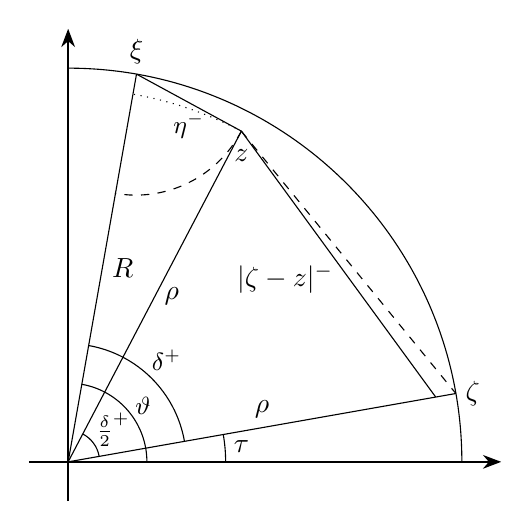
\begin{tikzpicture}
            \coordinate (zeta) at (4.924, 0.868);
            \coordinate (z) at (2.2, 4.2);
            \coordinate (xi) at (0.868, 4.924);
            \coordinate (auxiliary1) at ($(0,0)!0.948!(zeta)$);

            \draw[-{Stealth}, thick] (-0.5, 0) -- (5.5, 0);
            \draw[-{Stealth}, thick] (0, -0.5) -- (0, 5.5);
            \draw[thin] (5,0) arc[start angle=0, end angle=90, radius=5];
            \draw[thin] (0, 0) -- (zeta);
            \draw[thin] (0, 0) -- (xi);
            \draw[thin] (0, 0) -- (z);
            \draw[thin] (z) -- (xi);
            \draw[thin] (z) -- (auxiliary1);
            \draw[dashed, thin] (z) -- (zeta);
            \draw[thin] ($(0,0)!0.08!(zeta)$) arc[start angle=10, end angle=62.35, radius=0.4];
            \draw[thin] ($(0,0)!0.3!(zeta)$) arc[start angle=10, end angle=80, radius=1.5];
            \draw[thin] (2,0) arc[start angle=0, end angle=10, radius=2];
            \draw[thin] (1,0) arc[start angle=0, end angle=80, radius=1];
            \draw[dashed] (z) arc[start angle=-27.65, end angle=-100, radius=1.516];
            \draw[dotted] (z) arc[start angle=62.35, end angle=80, radius=4.741];

            \node[anchor=west] at (zeta) {\(\zeta\)};
            \node[anchor=north] at ([yshift=-3pt] z) {\(z\)};
            \node[anchor=south] at (xi) {\(\xi\)};
            \node[anchor=south] at ($(0,0)!0.5!(zeta)$) {\(\rho\)};
            \node[anchor=north] at ($(z)!0.5!(xi)$) {\small\(\eta^-\)};
            \node[anchor=west] at ($(0,0)!0.5!(xi)$) {\(R\)};
            \node[anchor=west] at ($(z)!0.5!(0,0)$) {\(\rho\)};
            \node[anchor=north] at (0.57,0.75) {\small \(\tfrac{\delta}{2}^+\)};
            \node[anchor=north] at (0.95,0.95) {\small\(\vartheta\)};
            \node[anchor=north] at (1.25,1.55) {\small\(\delta^+\)};
            \node[anchor=north] at (2.2,0.4) {\(\tau\)};
            \node[anchor=east] at ([yshift=-6pt, xshift=-2pt] $(z)!0.5!(zeta)$) {\(|\zeta-z|^-\)};
        \end{tikzpicture}
        \caption{\(\zeta\), \(\xi\), and \(z\) when \(\abs{\vartheta-\tau}>\delta\), with angles and distances marked. The use of \(+\) and \(-\) denote a value more or less (respectively) than the preceeding value.}
        \label{fig:dirichletproblemwithlaplaceequationsolution_secondintegral}
    \end{figure}By continuity of \(\varphi\) compact set \(\partial D(0,R)\), by \cref{thm:heinecantor}, it is bounded and \(M=\sup_{\qty|\zeta|=R}\abs{\varphi(\zeta)}\) is finite. The Poisson kernel can be rewritten as \[P(\zeta,z)=\frac{R^2-\rho^2}{2\piup\qty|\zeta-z|^2},\]
    where \(\zeta=R\ee^{\ii\tau}\) and \(z=\rho \ee^{\ii\theta}\), with \(\abs{\vartheta-\tau}>\delta\). Then \(\exists\eta>0\) such that \(\forall z\) with \(|\xi-z|<\eta\),
    \begin{equation}
        \abs{\theta-\tau}>\frac{\delta}{2}\label{eq:dirichletproblemwithlaplaceequationsolution_constraint1},
    \end{equation} and
    \begin{equation}
        \rho>\frac{R}{2}\Longrightarrow\eta\leq\frac{R}{2}\label{eq:dirichletproblemwithlaplaceequationsolution_constraint2}
    \end{equation} (these can be arbitrarily chosen for different resulting bounds) as in \cref{fig:dirichletproblemwithlaplaceequationsolution_secondintegral}. Then, \[|\zeta-z|^2>4\rho^2\sin[2](\frac{\delta}{4})>\frac{1}{2}R^2\qty(1-\cos(\frac{\delta}{2})).\]

    We aim to prove that \(\abs{I_2}<\varepsilon\). Since \(\abs{\varphi\qty(R\ee^{\ii\vartheta})-\varphi(\zeta)}<2M\), the condition is satisfied if \(\int_{\abs{\vartheta-\tau}>\delta}\frac{R^2-\rho^2}{\piup R^2\qty(1-\cos(\frac{\delta}{2}))}\dd{\tau}<2\frac{R^2-\rho^2}{R^2\qty(1-\cos(\frac{\delta}{2}))}< \frac{\varepsilon}{2M}\), and from rearrangement, we can tighten the constraint with:
    \begin{equation}
        R^2-\rho^2<\frac{\varepsilon}{4M}R^2\paren{1-\cos(\frac{\delta}{2})}\Longleftarrow R-\rho<\frac{\varepsilon}{8M}R\paren{1-\cos(\frac{\delta}{2})}.\label{eq:dirichletproblemwithlaplaceequationsolution_constraint3}
    \end{equation}
    From \cref{fig:dirichletproblemwithlaplaceequationsolution_secondintegral}, it is evident that \(R-\rho<|\xi-z|<\eta\). In order for \cref{eq:dirichletproblemwithlaplaceequationsolution_constraint1} to be true, we can enforce that \(\abs{\vartheta-\theta}<\frac{\delta}{2}\). In other words \(\abs{\xi-z}^2<R^2+\rho^2-2R\rho\cos(\frac{\delta}{2})\).

    Obviously, this is satisfied if \(|\xi-z|^2<\frac{R^2}{2}\paren{1-\cos(\frac{\delta}{2})}<2\rho^2\qty(1-\cos(\frac{\delta}{2}))\). This can be rearranged into \(|\xi-z|<\frac{R\sqrt{2}}{2}\sqrt{1-\cos(\frac{\delta}{2})}=R\sin\qty(\frac{\delta}{4})\). Therefore, we can choose \[\eta=\min\qty[\frac{\varepsilon}{8M}R\paren{1-\cos(\frac{\delta}{2})},R\sin\qty(\frac{\delta}{4}),\frac{R}{2}]>0,\] under which \cref{eq:dirichletproblemwithlaplaceequationsolution_constraint1,eq:dirichletproblemwithlaplaceequationsolution_constraint2,eq:dirichletproblemwithlaplaceequationsolution_constraint3} are satisfied.

    Hence, \(\forall\varepsilon>0\), \(\exists\eta>0\) such that \(\forall z\) with \(0<\abs{\xi-z}<\eta\), we have \(\abs{\varphi(\xi)-u(z)}<2\varepsilon\). Then \cref{eq:dirichletproblemwithlaplaceequationsolution_limittoboundary} follows.

    We will now show that \(u(z)\) is unique. Assume that \(v\not\equiv u\) on \(\overline{D(0,R)}\) also solves the problem. Then \(u-v\) is harmonic and vanishes on \(\partial D(0,R)\). By the Poisson Integral Formula (\cref{eq:poissonintegralformula2}), \(u(z)-v(z)=\int_0^{2\piup}P(\zeta,z)\qty[u(\zeta)-v(\zeta)]\dd{\tau}=0\) for all \(z\in D(0,R)\). Since \(u-v\) vanishes, we have a contradiction.
\end{proof}
\subsubsection{In Harmonic Analysis}
Consider \(R=1\), \(\zeta=\ee^{\ii\tau}\), and \(z=\rho \ee^{\ii\theta}\) in \cref{eq:poissonintegralformula2}:
\begin{gather}
    u(z)=\frac{1}{2\piup}\int_0^{2\piup} u(\zeta)\frac{1-\abs{z}^2}{\abs{\zeta-z}^2}\dd{\tau} = \frac{1}{2\piup}\int_0^{2\piup}\frac{\qty(1-\rho^2)u\qty(\ee^{\ii\tau})\dd{\tau}}{\qty(\ee^{\ii\tau}-\rho \ee^{\ii\theta})\qty(\ee^{-\ii\tau}-\rho \ee^{-\ii\theta})} \nonumber \\
    =\frac{1}{2\piup}\int_0^{2\piup} \frac{\qty(1-\rho^2)u\qty(\ee^{\ii\tau})\dd{\tau}}{1+\rho^2-2\rho\cos(\theta-\tau)}.\label{eq:poissonintegralformulatrigonometricsubstitution}
\end{gather}
Since \(u\qty(z)\) is continuous on \(\partial\mathbb{D}\) and \(u\circ\exp(\ii\theta)\) is periodic with period \(2\piup\), it admits a Fourier series representation
\begin{equation}
    u\qty(\ee^{\ii\theta})\sim\sum_{n=-\infty}^\infty a_n \ee^{\ii n\theta},\qquad a_n=\frac{1}{2\piup}\int_0^{2\piup} u\qty(\ee^{\ii\tau})\ee^{-\ii n\tau}\dd{\tau}. \label{eq:poissonintegralformulafourierseries}
\end{equation}
This series may diverge. Observe that continuity of \(u\) on the compact set \(\partial\mathbb{D}\) implies uniform boundedness: \(\exists M>0\) such that \(\abs{u\qty(\ee^{\ii\theta})} \leq M\) for all \(\theta\) (\cref{thm:continuousfunctionboundedoncompact}). Consequently, \(\abs{a_n} \leq M\). Introducing factors \(\rho^{\abs{n}}\) with \(\abs{\rho}<1\) yields a convergent series:
\[\sum_{n=-\infty}^\infty a_n \ee^{\ii n\theta}\rho^{\abs{n}}, \quad\abs{\sum_{n=-\infty}^\infty a_n \ee^{\ii n\theta}\rho^{\abs{n}}}\leq\sum_{n=-\infty}^\infty\abs{a_n}\rho^{\abs{n}}\leq M \frac{1+\abs{\rho}}{1-\abs{\rho}}.\]
Substituting the coefficients gives
\begin{align*}
    \sum_{n=-\infty}^\infty a_n \ee^{\ii n\theta}\rho^{\abs{n}} & =\sum_{n=-\infty}^\infty \qty(\frac{1}{2\piup}\int_0^{2\piup}u\qty(\ee^{\ii\tau})\ee^{-\ii n\tau}\dd{\tau}) \ee^{\ii n\theta}\rho^{\abs{n}} \\
    & =\frac{1}{2\piup} \sum_{n=-\infty}^\infty \int_0^{2\piup}\rho^{\abs{n}} u\qty(\ee^{\ii\tau}) \ee^{\ii n(\theta-\tau)}\dd{\tau}.
\end{align*}
By \cref{thm:weierstrassmtest,thm:limitintegralswitch},
\begin{equation}
    \frac{1}{2\piup}\sum_{n=-\infty}^\infty \int_0^{2\piup} \rho^{\abs{n}}u\qty(\ee^{\ii\tau}) \ee^{\ii n(\theta-\tau)} \dd{\tau}=\frac{1}{2\piup} \int_0^{2\piup} u\qty(\ee^{\ii\tau})\sum_{n=-\infty}^\infty \rho^{\abs{n}} \ee^{\ii n(\theta-\tau)}\dd{\tau}.\label{eq:poissonintegralformulafourierseriespostintegralsummationswitch}
\end{equation}
The summation simplifies as follows:
\begin{align*}
    \sum_{n=-\infty}^\infty \rho^{\abs{n}} \ee^{\ii n(\theta-\tau)} & =\sum_{n=0}^\infty \rho^n \ee^{\ii n(\theta-\tau)}+\sum_{n=1}^\infty \rho^n \ee^{-\ii n(\theta-\tau)} \\
    & =1+2\sum_{n=1}^\infty\rho^n\cos[n(\theta-\tau)]                                                    \\
    & =1+2\Re\sum_{n=1}^\infty\rho^n \ee^{\ii n(\theta-\tau)}                                            \\
    & =1+2\Re\qty[\frac{\rho \ee^{\ii(\theta-\tau)}}{1-\rho \ee^{\ii(\theta-\tau)}}]                     \\
    & =\frac{1-\rho^2}{1+\rho^2-2\rho\cos(\theta-\tau)}.
\end{align*}
Substituting into \cref{eq:poissonintegralformulafourierseriespostintegralsummationswitch} yields
\[\sum_{n=-\infty}^\infty a_n \ee^{\ii n\theta}\rho^{\abs{n}}=\frac{1}{2\piup}\int_0^{2\piup}\frac{\qty(1-\rho^2)u\qty(\ee^{\ii\tau})}{1+\rho^2-2\rho\cos(\theta-\tau)}\dd{\tau}=u\qty(\rho \ee^{\ii\theta}).\]
Furthermore, by the proof of \cref{thm:dirichletproblemwithlaplaceequationsolution} (specifically \cref{eq:dirichletproblemwithlaplaceequationsolution_limittoboundary}),
\[\lim_{\rho\to1^-}\sum_{n=-\infty}^\infty a_n \ee^{\ii n\theta}\rho^{\abs{n}}=u\qty(\ee^{\ii\theta}).\]
Thus, for any continuous function \(u\) on \(\partial\mathbb{D}\), its Fourier series is \textscsl{Abel summable} to \(u\).

We now establish that real-valued continuous functions satisfying the mean-value property are harmonic.
\begin{theorem}\label{thm:meanvaluepropertysolutionsareharmonic}
    Let \(U\subseteq\mathbb{C}\) be open and \(f:U\to\mathbb{R}\) continuous. Suppose for every \(z_0\in U\), there exists \(\lambda>0\) with \(\overline{D\qty(z_0,\lambda)}\subseteq U\) such that for all \(0<\varepsilon\leq\lambda\),
    \[f(z_0)=\frac{1}{2\piup}\int_0^{2\piup} f\qty(z_0+\varepsilon \ee^{\ii t})\dd{t}.\]
    Then \(f\) is harmonic on \(U\).
\end{theorem}
\begin{proof}
    Fix \(z_0\in U\) arbitrarily and choose \(\lambda>0\) such that \(\overline{D\qty(z_0,\lambda)}\subset U\). Because \(f\in C^0\qty(\partial D\qty(z_0,\lambda))\), \cref{thm:dirichletproblemwithlaplaceequationsolution} guarantees the existence of a unique harmonic function \(u\) on \(D\qty(z_0,\lambda)\) satisfying
    \[u(z)=\int_0^{2\piup}f(\zeta)P\qty(\zeta,z) \dd{\tau},\]
    with \(u=f\) on \(\partial D\qty(z_0,\lambda)\). Define \(\psi=f-u\) on \(\overline{D\qty(z_0,\lambda)}\). Then \(\psi\) is continuous, satisfies the mean-value property, and vanishes on \(\partial D\qty(z_0,\lambda)\). By the proof of \cref{thm:maximummodulus}, which relies solely on the mean-value property, \(\psi\equiv 0\) on \(\overline{D\qty(z_0,\lambda)}\). Thus, \(f\equiv u\) on \(\overline{D\qty(z_0,\lambda)}\), implying \(f\) is harmonic at \(z_0\). The arbitrariness of \(z_0\) establishes harmonicity on \(U\).
\end{proof}
\section{The Theory of Weierstrass}
While Weierstrass' contributions in complex analysis are mainly characterized by his discoveries on uniform convergence, he also characterized entire and \textscsl{meromorphic functions} and a unique representation of entire functions, as well as his contributions toward the study of \textscsl{essential singularities}.

To classify the behavior of non-removable singularities, mathematicians generalized Taylor series to \textscsl{Laurent series}.
\subsection{Laurent Series}
The Laurent series generalizes the Taylor series to holomorphic functions with isolated singularities. While Taylor series are valid within a disk centered at a point of holomorphy, Laurent series apply to annular regions surrounding a singularity, making them essential for studying functions near non-removable singularities (refer to \cref{thm:riemannremovablesingularities}).

We now introduce a fundamental result in complex analysis due to Weierstrass, which formalizes the conditions under which the limit of a sequence of holomorphic functions is itself holomorphic. This theorem not only guarantees the holomorphy of the limit function but also the uniform convergence of its derivatives (its statement was used in the proof of \cref{thm:hurwitzsimplecase}).
\begin{theorem}[Weierstrass]\label{thm:weierstrassconvergence}
    Let \(\cbraces{f_n(z)}_{n\in\mathbb{N}}\) be a sequence of holomorphic functions on an open region \(U\subseteq\mathbb{C}\) that converges uniformly to \(f(z)\) on every compact subset of \(U\). Then \(f(z)\) is holomorphic on \(U\), and \(\forall k\in\mathbb{N}\), the sequence \(\cbraces{f^{(k)}_n(z)}_{n\in\mathbb{N}}\) uniformly converges to \(f^{(k)}(z)\) on all compact subsets of \(U\).
\end{theorem}
\begin{proof}
    By Morera's Theorem (\cref{thm:morera}) and the uniform convergence of \(\qty{f_n(z)}\), the holomorphy of \(f(z)\) follows (refer to \cref{eq:hurwitzsimplecase_integrallimitswitchforholomorphy} and preceding explanations).

    Following the same logic, by \cref{cor:nthderivativeboundedsupremum}, \(\forall k\in\mathbb{N}\) and for all compact \(K\subset U\) and open \(V\supset K\) relatively compact in \(U\) there exists a finite constant \(c_k>0\) such that
    \[\lim_{n\to\infty}\sup_{z\in K}\abs{f_n^{(k)}(z)-f^{(k)}(z)}\leq c_k\lim_{n\to\infty}\sup_{z\in V}\abs{f_n(z)-f(z)}.\] Since \(\cbraces{f_n(z)}\) is uniformly convergent, the limit on the right-hand side vanishes. Then,
    \[\lim_{n\to\infty}\sup_{z\in K}\abs{f_n^{(k)}(z)-f^{(k)}(z)}=0,\] and therefore \(\qty{f^{(k)}_n(z)}\) uniformly converges on all compact subsets of \(U\).
\end{proof}
The condition of uniform convergence on every compact subset can also be significantly loosened, by the fact demonstrated below:
\begin{proposition}
    Let \(U\subseteq\mathbb{C}\) be an open bounded region, and let \(\qty{f_n(z)}\) be holomorphic on \(U\). Let \(K\subset U\) be compact. If \(f_n\rightrightarrows f\) on \(\partial K\), then \(f_n\rightrightarrows f\) on \(K\).
\end{proposition}
\begin{proof}
    By the converse statement of the Cauchy Criterion (\cref{thm:cauchycriterionuniformconvergence}), \(\forall\varepsilon>0\), \(\exists N\in\mathbb{N}\) such that \(\forall n,m>N\), \[\sup_{z\in\partial K}\qty|f_n(z)-f_m(z)|<\varepsilon.\]
    By the Maximum Modulus Principle (\cref{thm:maximummodulus}) on \(f_n-f_m\), \[\sup_{z\in\partial K}\abs{f_n(z)-f_m(z)}=\sup_{z\in K}\abs{f_n(z)-f_m(z)}<\varepsilon.\]
    It follows that \(f_n\rightrightarrows f\) on \(K\) by \cref{thm:cauchycriterionuniformconvergence}.
\end{proof}
\begin{remark}
    From the above result, the uniform convergence on every compact subset in \cref{thm:weierstrassconvergence} can therefore be loosened to the uniform convergence on every simple closed curve.
\end{remark}
We will now study Laurent series. Let \(a\in\mathbb{C}\) and \(\qty{c_n}_{n\in\mathbb{Z}}\subset\mathbb{C}\) be constants. A series in the form of
\begin{equation}\label{eq:laurentseries}
    f(z)=\sum_{n=-\infty}^\infty c_n(z-a)^n
\end{equation}
is a Laurent series at the point \(a\). The series can be separated into a power series with non-negative exponents,
\begin{equation}
    \varphi(z)=\sum_{n=0}^\infty c_n(z-a)^n,\label{eq:laurentseriesnonnegativeexponents}
\end{equation} and a power series with negative exponents,
\begin{equation}
    \psi(z)=\sum_{n=1}^{\infty}c_{-n}(z-a)^{-n}.\label{eq:laurentseriesnegativeexponents}
\end{equation} \cref{eq:laurentseries} is said to be convergent at \(z=z_0\) if the two power series are both convergent. Let the convergence radius of \cref{eq:laurentseriesnonnegativeexponents} be \(R=\frac{1}{\varlimsup_{n\to\infty}\sqrt[n]{\abs{c_n}}}\) by the Cauchy--Hadamard Theorem (\cref{thm:cauchyhadamard}). It follows that the \(\varphi\) is holomorphic on \(D(a,R)\). Let \(\zeta=(z-a)^{-1}\). Then \cref{eq:laurentseriesnegativeexponents} becomes \(\sum_{n=1}^\infty c_{-n}\zeta^n\). This series converges when \(\abs{\zeta}<\frac{1}{\varlimsup_{n\to\infty}\sqrt[n]{\abs{c_{-n}}}}=\lambda\). Let \(r=\frac{1}{\lambda}\). Then \(\psi(z)\) converges when \(\abs{z-a}>\varlimsup_{n\to\infty}\sqrt[n]{\abs{c_{-n}}}\), or when \(z\in\mathbb{C}\setminus\overline{D(a,r)}\).

If \(R>r\), then \(f\) is convergent on the annulus \(D(a,R)\setminus\overline{D(a,r)}\) and divergent on \(\mathbb{C}\setminus\overline{D(a,R)}\cup D(a,r)\). If \(r=R\), the series diverges possibly everywhere but on \(\partial D(a,r)\). Similar to power series with positive exponents, the convergence on the boundary varies. For example, \(\sum_{\substack{n=-\infty\\n\neq0}}^\infty\frac{z^n}{n^2}\), where \(R=r=1\), converges (absolutely) on \(\partial\mathbb{D}\), whereas \(\sum_{n=-\infty}^\infty z^n\) diverges on all of \(\partial\mathbb{D}\), while \(\sum_{\substack{n=-\infty\\n\neq0}}^\infty\frac{z^n}{n}\) converges (conditionally) on all of \(\partial\mathbb{D}\setminus\qty{1}\) and diverges at \(z=1\). If \(r>R\), then the series is divergent on all of \(\mathbb{C}\). The region \(D(a,R)\setminus\overline{D(a,r)}\) is known as the \textscsl{annulus of convergence}.\ \(f(z)\) in \cref{eq:laurentseries} is holomorphic over this annulus. The series \(\varphi(z)\) is known as the \textscsl{holomorphic part} of \(f(z)\), and \(\psi(z)\) is known as the \textscsl{principal part} of the Laurent series. The properties of the convergence disk in Abel's Theorem (\cref{thm:abelradius}) can be generalized to Laurent series. In other words, \(f\) is absolutely convergent on the annulus and is uniformly convergent on every compact subset of it.
\begin{theorem}\label{thm:laurentexpansionofholomorphicfunction}
    Let \(V=\cbraces{z\in\mathbb{C}}{r<\abs{z-a}<R}\) for some \(0\leq r<R\leq\infty\). Let \(f\) be holomorphic on \(V\). Then \(f\) has the unique \textscsl{Laurent expansion}
    \begin{equation}
        f(z)=\sum_{n=-\infty}^\infty c_n(z-a)^n,\qquad c_n=\frac{1}{2\piup\ii}\oint_{\gamma}\frac{f(\zeta)\ddzeta}{(\zeta-a)^{n+1}},\label{eq:laurentexpansionofholomorphicfunction_statement}
    \end{equation} for \(z\in V\) and any simple closed curve \(\gamma\subset V\) enclosing \(a\).
\end{theorem}
\begin{proof}
    \begin{figure}
        \centering
        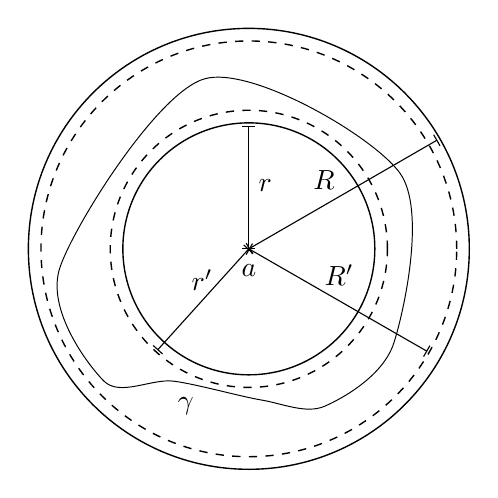
\begin{tikzpicture}\draw[line width=0.35] plot[smooth cycle] coordinates {
                (-2.4,-0.24) (-1.84,-1.68) (-0.96,-1.68) (0.16,-1.92) (0.96,-2.0) (1.84,-1.2) (1.92,0.96) (-0.56,2.16)
            };
            \draw[line width=0.5] (2.8,0) arc[start angle=0, end angle=360, radius=2.8];
            \draw[line width=0.5, dashed] (2.64,0) arc[start angle=0, end angle=360, radius=2.64];
            \draw[line width=0.5] (1.6,0) arc[start angle=0, end angle=360, radius=1.6];
            \draw[line width=0.5, dashed] (1.76,0) arc[start angle=0, end angle=360, radius=1.76];
            \draw[thin, |-|, line cap=round, shorten >=1pt] (0,0) -- (2.424,1.4) node[midway, anchor=south east, yshift=-2pt] {\(R\)};
            \draw[thin, |-|, line cap=round, shorten >=1pt] (0,0) -- (0,1.6) node[midway, right] {\(r\)};
            \draw[thin, |-|, line cap=round, shorten >=1pt] (0,0) -- (2.296,-1.32) node[midway, anchor=south, yshift=2pt] {\(R'\)};
            \draw[thin, |-|, line cap=round, shorten >=1pt] (0,0) -- (-1.184,-1.312) node[midway, anchor=south] {\(r'\)};

            \node[anchor=north] at (0,-0.08) {\(a\)};
            \node[anchor=north] at (-0.8,-1.76) {\(\gamma\)};
        \end{tikzpicture}
        \caption{The annulus \(V\), with \(\gamma_1\), \(\gamma_2\), and \(\gamma\).}\label{fig:laurentexpansionofholomorphicfunction}
    \end{figure}By the openness of \(V\), there exist two circles \(\gamma_1\subset V\) with radius \(r'\) and \(\gamma_2\subset V\) with radius \(R'\) centered at \(a\) such that \(\gamma\) encloses \(\gamma_1\) and \(\gamma_2\) encloses \(\gamma\) both without intersection. Let \(W=\cbraces{z\in V}{r'<|z-a|<R'}\) and \(z\in W\) be arbitrary. By the Cauchy--Goursat Formula (\cref{thm:cauchygoursatformula}), \[f(z)=\frac{1}{2\piup\ii}\qty(\oint_{\gamma_2}\frac{f(\zeta)\ddzeta}{\zeta-z}-\oint_{\gamma_1}\frac{f(\zeta)\ddzeta}{\zeta-z}).\]
    \(\forall\zeta\in\gamma_1\) (or \(|\zeta-a|=r'\)), \(\abs{\zeta-a}<\abs{z-a}\) and therefore, \(\frac{\abs{\zeta-a}}{\abs{z-a}}<1\). It follows that
    \begin{equation}
        \frac{1}{\zeta-z}=-\frac{1}{(z-a)\qty(1-\frac{\zeta-a}{z-a})}=-\sum_{n=0}^\infty\frac{\qty(\zeta-a)^n}{\qty(z-a)^{n+1}}\label{eq:laurentexpansionofholomorphicfunction_kernelexpansioninside}
    \end{equation} is uniformly convergent with respect to \(\zeta\). Similarly, \(\forall\zeta\in\gamma_2\), \(\abs{\zeta-a}>\abs{z-a}\Leftrightarrow\frac{\abs{z-a}}{\abs{\zeta-a}}<1\), and it follows that
    \begin{equation}
        \frac{1}{\zeta-z}=\frac{1}{(\zeta-a)\qty(1-\frac{z-a}{\zeta-a})}=\sum_{n=0}^\infty\frac{\qty(z-a)^n}{\qty(\zeta-a)^{n+1}}\label{eq:laurentexpansionofholomorphicfunction_kernelexpansionoutside}
    \end{equation} is uniformly convergent with respect to \(\zeta\). By the boundedness of \(f\) on \(\gamma_1\) and \(\gamma_2\) from holomorphy on a compact set, and from the Weierstrass \(M\)--Test (\cref{thm:weierstrassmtest}), we get that
    \begin{equation}
        f(z)=\frac{1}{2\piup\ii}\qty(\sum_{n=0}^\infty\oint_{\gamma_2}\frac{(z-a)^n}{(\zeta-a)^{n+1}}f(\zeta)\ddzeta+\sum_{n=1}^\infty\oint_{\gamma_1}\frac{(\zeta-a)^{n-1}}{(z-a)^{n}}f(\zeta)\ddzeta).\label{eq:laurentexpansionofholomorphicfunction_finalstep}
    \end{equation}
    By the Cauchy--Goursat Theorem (\cref{thm:cauchygoursattheorem}), for a given \(n\), \[\int_{\gamma_2^+\cup\gamma^-}\frac{f(\zeta)\ddzeta}{(\zeta-a)^n}=0\qand\int_{\gamma^+\cup\gamma_1^-}f(\zeta)(\zeta-a)^n\ddzeta=0.\]
    In other words, the integrals in \cref{eq:laurentexpansionofholomorphicfunction_finalstep} are the same as on \(\gamma\). Hence, we get that \[f(z)=\sum_{n=0}^\infty c_n(z-a)^n+\sum_{n=1}^\infty c_{-n}(z-a)^{-n}=\sum_{n=-\infty}^\infty c_n(z-a)^n.\]
    The constants \(\qty{c_n}_{n\in\mathbb{Z}}\) are also unique in the expansion. For the sake of contradiction, assume there exists another set of constants \(\qty{c'_n}_{n\in\mathbb{Z}}\) such that
    \begin{equation}
        f(z)=\sum_{n=-\infty}^\infty c'_n{(z-a)}^n,\label{eq:laurentexpansionofholomorphicfunction_uniquenessstatement}
    \end{equation}
    where \(z\in V\) and the series is uniformly convergent on \(\gamma\). Let \(m\in\mathbb{Z}\) be arbitrary. ByCauchy--Goursat (\cref{thm:cauchydifferentiationformula}), \[\oint_{\gamma}(z-a)^k\ddz=
        \begin{cases}
            0                      &\qif* k\geq0   \\
            2\piup\ii\dv[-k-1]{z}(1) &\qif* k\leq -1
        \end{cases}=
        \begin{cases}
            0       &\qif* k\neq-1 \\
            2\piup\ii &\qif* k=-1    \\
    \end{cases}.\]
    Multiplying \cref{eq:laurentexpansionofholomorphicfunction_uniquenessstatement} by \((z-a)^{-m-1}\) and from integrating over \(\gamma\), we get that \[\oint_\gamma\frac{f(z)\ddz}{(z-a)^{m+1}}=\oint_{\gamma}\sum_{n=-\infty}^\infty c'_n(z-a)^{n-m-1}\ddz,\] implying that \[2\piup \ii c_m=\sum_{n=-\infty}^\infty c'_n\oint_{\gamma}(z-a)^{n-m-1}\ddz=2\piup\ii c'_m,\]
    which is a contradiction, implying uniqueness.
\end{proof}
\begin{remark}
    Unlike Taylor series, Laurent series \textit{are not} necessarily unique up to the point of expansion. Depending on the chosen annulus, the expansion may differ.
\end{remark}
\subsection{Isolated Singularities}
An \textscsl{isolated singularity} of a complex function is a point \(a\in\mathbb{C}\) where a function \(f\) is holomorphic on some open punctured neighborhood of \(a\) (namely, for some \(r>0\), the punctured disk \(D^*(a,r)\)), but not necessarily defined or holomorphic at \(a\) itself. The nature of this isolated singularity is characterized by the principal part \(\psi(z)\) (let \(\varphi(z)\) be the holomorphic part) of the Laurent series of \(f\) at the point \(a\). Specifically, we can analyze the behavior of \(f(z)\) as \(z\to a\).
\begin{enumerate}
    \item\label{itm:isolatedsingularities_removable} If \(\lim_{z\to a}f(z)\) exists and is finite, then \(z=a\) is a removable singularity and can be analytically continued to \(D(a,r)\) by \cref{thm:riemannremovablesingularities}. Consequently, \(f(z)\) has a convergent Taylor expansion and the principal part of its Laurent expansion vanishes, and \(f(z)=\varphi(z)\).
    \item\label{itm:isolatedsingularities_pole} If \(\lim_{z\to a}f(z)=\infty\), then \(z=a\) is a \textscsl{pole} of \(f\) (from the stereographic projection and the Riemann sphere, the \(\infty\) is a single point in \(\extcomplex\), and approaching \(\infty\) does not distinguish between different directions, unlike the use of \(+\infty\) and \(-\infty\)).
        \begin{theorem}\label{thm:isolatedsingularities_pole_laurentexpansion}
            The condition \(\lim_{z\to a}f(z)=\infty\) is equivalent to there being a finite number of nonzero \(c_{-n}\)'s, where \(n\in\mathbb{N}\).
        \end{theorem}
        In other words the principal part of \(f\) is equal to \[\psi(z)=\frac{c_{-1}}{z-a}+\cdots+\frac{c_{-m}}{(z-a)^m}\quad c_{-m}\neq0\] for some \(m\in\mathbb{N}\). Therefore, \(f(z)=\varphi(z)+\psi(z)=\sum_{n=-m}^\infty c_n(z-a)^n=\frac{g(z)}{(z-a)^m}\) on the punctured disk \(D^*(a,r)\), where \(g(z)=\sum_{n=0}^\infty c_{n-m}(z-a)^n\) is holomorphic on \(D(a,r)\) and does not attain a zero at \(z=a\). Then \(f(z)\) has a pole at \(z=a\) with order \(m\). If \(m=1\), the pole is also called a \textscsl{simple pole}.
        \begin{proof}
            Obviously, under the assumption of a finite, nonempty number of non-negative terms in the principal part of the Laurent expansion coefficients, \(\lim_{z\to a}f(z)\to\infty\). Now we will prove the converse. Let \(g(z)=\frac{1}{f(z)}\). Then \(\lim_{z\to a}g(z)=0\). There exists a \(\delta>0\) such that \(f\) is nonzero on \(D^*(a,\delta)\). Then \(g(z)\) is holomorphic on \(D^*(a,\delta)\) and has a removable singularity at \(z=a\). By \cref{thm:riemannremovablesingularities}, \(g\) can be analytically continued to \(D^*(a,\delta)\). Let the multiplicity of the zero at \(z=a\) be \(m\). Then \(g(z)=\phi(z)(z-a)^m\), where \(\phi(z)\) is holomorphic and nonzero at \(z=a\). Then there exists a \(\delta'>0\) such that \(\phi\) is nonzero on \(D(a,\delta')\). It follows that \(\frac{1}{\phi}\) is holomorphic and nonzero on \(D(a,\delta')\). We can then write its Taylor expansion as \[\frac{1}{\phi(z)}=c_{-m}+c_{1-m}(z-a)+\cdots,\]
            where \(c_{-m}\neq0\). It follows that \[f(z)=\frac{1}{g(z)}=\frac{(z-a)^{-m}}{\phi(z)}={c_{-m}}(z-a)^{-m}+c_{1-m}(z-a)^{1-m}+\cdots+c_0+\cdots.\]
            By the uniqueness of the Laurent series (by \cref{thm:laurentexpansionofholomorphicfunction}), the conclusion follows.
        \end{proof}
    \item\label{itm:isolatedsingularities_essential} If \(\lim_{z\to a}f(z)\) is nonexistent, then \(a\) is known as an \textscsl{essential singularity}.
        \begin{example}\label{ex:isolatedsingularities_essential_exp1z}
            The function \(\ee^{\frac{1}{z}}\) has an essential singularity at \(z=0\).
        \end{example}
        \begin{proof}
            Observe that \(\lim_{\substack{z\to 0\\z\in\mathbb{R}_{>0}}}=\infty\). Similarly, \(\lim_{\substack{z\to0\\z\in\mathbb{R}_{<0}}}=0\), and \(\lim_{\substack{z\to0\\z\in \ii\mathbb{R}_{>0}}}\) is divergent. Therefore, the limit does not exist.
        \end{proof}
        The implication on its Laurent expansion at \(a\) is:
        \begin{theorem}
            The necessary and sufficient for \(\lim_{z\to a} f(z)\) to not exist is that infinitely many of \(c_{-n}\) (where \(n\in\mathbb{N}\)) are nonzero.
        \end{theorem}
        This follows by elimination from the established trichotomy; if the limit as \(z\to a\) does not exist, then the singularity is neither removable nor a pole (results from \ref{itm:isolatedsingularities_removable} and \ref{itm:isolatedsingularities_pole}). Similar logic can be applied to the coefficients of the Laurent expansion.

        Indeed, in \cref{ex:isolatedsingularities_essential_exp1z}, the Laurent expansion is equal to:
        \[\ee^{\frac{1}{z}}=\sum_{n=0}^\infty\frac{z^{-n}}{n!},\]
        which has infinitely many nonzero coefficients of negative powers.
\end{enumerate}
A function with an essential singularity exhibits striking behavior. We will first introduce the following famous result.
\begin{theorem}[name=\textsc{Casorati--Sokhotski--Weierstrass},store=thm:casoratiweierstrass]\label{thm:casoratiweierstrass}
    Let \(a\in\mathbb{C}\) and \(U\subseteq\mathbb{C}\) be an open region. Suppose \(f:U\setminus\qty{a}\to\mathbb{C}\) is holomorphic with an essential singularity at \(a\). Then the set of values that \(f\) attains on any open punctured neighborhood of \(a\) is dense. In other words, \(\forall\varepsilon,\delta>0\), \(\forall w\in\mathbb{C}\), \(\exists z\in D^*(a,\delta)\) such that \(|f(z)-w|<\varepsilon\).
\end{theorem}
\begin{proof}
    Assume for the sake of contradiction that \(\exists\varepsilon,\delta>0\), and \(\exists w\in\mathbb{C}\) such that \(\forall z\in D^*(a,\delta)\), \(|f(z)-w|>\varepsilon\). Define the auxiliary function \(g(z)=\frac{f(z)-w}{z-a}\), which is holomorphic and non-vanishing on the punctured neighborhood of \(a\). Since as \(z\to a\), \(g(z)\to\infty\), it follows that \(g(z)\) has a pole at \(a\). Let the order of the pole be \(m\in\mathbb{N}\). By \cref{thm:isolatedsingularities_pole_laurentexpansion}, \(g(z)\) has the Laurent expansion of \[\frac{c_{-m}}{(z-a)^m}+\cdots c_0+c_1(z-a)+\cdots\]
    for some \(m\in\mathbb{N}\). It follows that \[f(z)=\frac{c_{-m}}{(z-a)^{m-1}}+\cdots+c_{-1}+w+c_0(z-a)+\cdots.\] If \(m=1\), then \(f\) has a removable singularity at \(a\). If \(m\geq2\), then \(f\) has a pole at \(a\). Hence, we have a contradiction.
\end{proof}
An analogous proof yields the following result for entire functions.
\begin{theorem}\label{thm:casoratiweierstrassentire}
    The set of values that a non-constant entire function \(f\) assumes is dense in \(\mathbb{C}\).
\end{theorem}
\begin{proof}
    For the sake of contradiction, assume there exists \(w\in\mathbb{C}\) and \(\varepsilon>0\) such that \(D(w,\varepsilon)\notin f\qty(\mathbb{C})\). Define \(g(z)=\frac{1}{f(z)-w}\). It follows that \(\abs{g}\leq\frac{1}{\varepsilon}\) on \(\mathbb{C}\). By Liouville's Theorem (\cref{thm:liouville}), \(g\) is a constant function, and hence, \(f\) is also constant, which is a contradiction of the statement.
\end{proof}
In \cref{sec:differentialgeometry}, we will prove a profound generalization of the two results (\cref{thm:greatpicard} and \cref{thm:littlepicard}), which was first proved by Émile Picard in 1879:
\getkeytheorem{thm:littlepicard}
\getkeytheorem{thm:greatpicard}
\subsubsection{At the \texorpdfstring{\(\infty\)}{Infinity} Point}
Given the one-point compactification of \(\mathbb{C}\), \(\extcomplex\), we can now define and analyze the behavior of functions near the point at infinity. Similar to the classification of isolated singularities in \(\mathbb{C}\), we can classify \(\infty\) as a removable singularity, a pole, or an essential singularity of a holomorphic function.

Let \(f:\mathbb{C}\setminus\overline{D(0,R)}\to\mathbb{C}\) be holomorphic for some \(R>0\). Then \(z=\infty\) is an \textscsl{isolated singularity} of \(f\). To analyze the nature of the singularity, let \(\zeta=\frac{1}{z}\). We define a new function \(g(\zeta)=f\qty(\frac{1}{\zeta})=f(z)\), which is holomorphic on \(D^*\qty(0,\frac{1}{R})\). Then at \(\zeta=0\), \(g(\zeta)\) has the Laurent expansion of \[g(\zeta)=\sum_{n=-\infty}^\infty c_{-n}\zeta^n=\sum_{n=0}^\infty c_{-n}\zeta^n+\sum_{n=1}^\infty c_{n}\zeta^{-n}=\varphi(\zeta)+\psi(\zeta),\]
where \(\varphi\) and \(\psi\) are the holomorphic and principal parts of \(g\), respectively. Let \(\widetilde{\varphi}(z)=\varphi\qty(\frac{1}{z})\), \(\widetilde{\psi}(z)=\psi\qty(\frac{1}{z})\). At \(z=0\), \(f\) then has the Laurent expansion of \[f(z)=\sum_{n=-\infty}^\infty c_nz^n=\sum_{n=0}^\infty c_{-n}z^{-n}+\sum_{n=1}^\infty c_nz^n=\widetilde{\varphi}(z)+\widetilde{\psi}(z).\]

The classification of the singularity at \(\infty\) is then reduced to the classification of the singularity of \(g\) at \(0\):
\begin{enumerate}
    \item If \(z=\infty\) is a removable singularity of \(f(z)\), then \(f(z)\) has the form of \[f(z)=c_0+\frac{c_{-1}}{z}+\frac{c_{-2}}{z^2}+\frac{c_{-3}}{z^3}+\cdots.\]
    \item If \(z=\infty\) is a pole of \(f(z)\) with degree \(m\in\mathbb{N}\), then \(f(z)\) can be written as \[f(z)=c_{m}z^m+c_{m-1}z^{m-1}+\cdots+c_0+\frac{c_{-1}}{z}+\cdots,\] where \(c_{m}\neq0\).
    \item If \(z=\infty\) is an essential singularity of \(f(z)\), then \(f(z)\) can be expanded as \[f(z)=\sum_{n=-\infty}^\infty c_{n}z^n,\]
        where \(\forall N\in\mathbb{N}\), \(\exists n>N\) such that \(c_{n}\neq0\) (infinitely many coefficients of \(\psi\) or \(\widetilde{\psi}\) are nonzero).
\end{enumerate}
\begin{remark}
    Under stereographic projection from the point \(\mqty(0\\0\\1)\) of the unit sphere \(S_2\), a neighborhood of that point maps to a subset of the extended complex plane of the form \(\extcomplex\setminus K\), where \(K\) is a compact and connected subset of \(\mathbb{C}\). Such sets are referred to as \textscsl{neighborhoods of \(\infty\)} in the Riemann sphere.
\end{remark}
\begin{example}
    The function \(z\mapsto\frac{1}{z}\) has a removable singularity at \(z=\infty\), the function \(z\mapsto z^2\) has a pole at \(z=\infty\), and \(z\mapsto \ee^z\) has an essential singularity at \(z=\infty\).
\end{example}
\subsection{Entireness and Meromorphy}
We have previously defined the concept of an entire function in \cref{sec:complexdifferentiation}. Let \(f\) be entire with the unique Taylor expansion \(\sum_{n=0}^\infty c_nz^n\). Since \(z=\infty\) is an isolated singularity, by the uniqueness of the Laurent expansion, the expansion at \(z=0\) has the same form as the expansion at \(z=\infty\). We will now analyze the implications on the entire function \(f\) given an isolated singularity.
\begin{enumerate}
    \item If the infinity point is a removable singularity, then \(\lim_{z\to\infty} f(z)\) exists and is finite.
        \begin{proposition}\label{prop:removablesingularityatinftyentireconstant}
            If \(f(z)\) is entire and has a removable singularity at \(z=\infty\), then \(f\) is constant.
        \end{proposition}
        \begin{proof}
            Let \(z=\frac{1}{\zeta}\), \(g(\zeta)=f\qty(\frac{1}{\zeta})\), which has a removable singularity at \(\zeta=0\). By \cref{thm:riemannremovablesingularities}, \(g\) can be analytically continued to all of \(\mathbb{C}\), especially at \(\zeta=0\). Let \(w=g(0)\). Then, \(\forall\varepsilon>0\), \(\exists\delta>0\) such that \(\forall\zeta\in D(0,\delta)\), \(|g(\zeta)-w|<\varepsilon\). It follows that \(\forall \abs{z}>\frac{1}{\delta}\), \(\abs{f(z)}<|w|+\varepsilon\), and is bounded. For the complement, \(\forall z\in \overline{D\qty(0,\frac{1}{\delta})}\), \(f(z)\) is continuous on a compact set, and by \cref{thm:continuousfunctionboundedoncompact}, is also bounded.

            Then by Liouville's Theorem (\cref{thm:liouville}), \(f\) is constant.
        \end{proof}
    \item If \(f(z)\) has a pole at \(z=\infty\) of order \(m\in\mathbb{N}\), then \(f\) is a polynomial of degree \(m\).
        \begin{proof}
            By the classification of a pole at \(\infty\), \(f\) can be written as \[f(z)=c_mz^m+c_{m-1}z^{m-1}+\cdots+c_0+\frac{c_{-1}}{z}+\cdots.\]
            Since \(f(z)\) is entire, it is holomorphic at \(z=0\) and has a convergent Taylor expansion. By the uniqueness of Laurent expansions (\cref{thm:laurentexpansionofholomorphicfunction}), the two expansions are equivalent and therefore all terms with negative exponents vanish, and \[f(z)=c_mz^m+c_{m-1}z^{m-1}+\cdots+c_0,\]
            and since \(c_m\neq0\), the statement is confirmed.
        \end{proof}
    \item If \(f(z)\) has an essential singularity at \(z=\infty\), \(f(z)\) is known as a \textscsl{transcendental entire function}.
\end{enumerate}
\begin{example}
    The entire functions \(\sin(z)\), \(\cos(z)\), \(\sinh(z)\), \(\cosh(z)\), and \(\exp(z)\) are transcendental.
\end{example}
\begin{definition}[Meromorphy]\label{def:meromorphicfunction}
    Let \(U\subseteq\mathbb{C}\) be open, and let \(\cbraces{a_n}_{n\in\mathbb{N}}\subset U\) be a set of isolated points. Suppose \(f:U\setminus\cbraces{a_n}_{n\in\mathbb{N}}\to\mathbb{C}\) is holomorphic and has a pole at each of \(z\in\qty{a_n}\). Then \(f\) is \textscsl{meromorphic} in \(U\).
\end{definition}
Similar to holomorphy, meromorphy on a compact set can be defined as meromorphy on a neighborhood of the set. In general, we imply for the set to be open unless stated otherwise. If the set is not implicitly specified, we assume meromorphy on \(\mathbb{C}\).

All holomorphic functions are meromorphic functions (with poles on \(\emptyset\)). Consequently, entire functions are meromorphic on \(\mathbb{C}\). All rational functions (including polynomials) are also meromorphic on \(\mathbb{C}\). In the study of meromorphic functions with an isolated singularity at \(\infty\), rational functions are of important interest.

Let \(f(z)\) be rational, written as \(f(z)=\frac{p(z)}{q(z)}\), where \(p\) and \(q\) are polynomials. Let
\begin{gather*}
    p(z)=a_nz^n+a_{n-1}z^{n-1}+\cdots a_0\\
    q(z)=b_mz^m+b_{m-1}z^{m-1}+\cdots b_0,
\end{gather*} where \(a_n,b_m\neq 0\). Trivially, the poles of \(f\) are the zeros of \(q\). Since \[f(z)=\frac{z^n}{z^m}\cdot\frac{a_n+\frac{a_{n-1}}{z}+\cdots+\frac{a_0}{z^n}}{b_m+\frac{b_{m-1}}{z}+\cdots\frac{b_0}{z^m}},\] we have \[\lim_{z\to\infty} f(z)=
    \begin{cases}
        \frac{a_n}{b_m} &\qif* n=m \\
        0               &\qif* n<m \\
        \infty          &\qif* n>m
\end{cases}.\]
Conversely, we have:
\begin{theorem}\label{thm:rationalmeromorphicfunctions}
    If \(f(z)\) is meromorphic on \(\mathbb{C}\) and has a pole or removable singularity at \(z=\infty\), then \(f\) is a rational function.
\end{theorem}
\begin{proof}
    Since \(f\) is meromorphic on \(\mathbb{C}\), its singularities are isolated poles. The assumption that \(f\) has either a pole or a removable singularity at \(\infty\) implies that this singularity is also isolated. Thus, there exists some \(R>0\) such that \(f\) is holomorphic on the punctured neighborhood \(\cbraces{z\in\mathbb{C}}{R<|z|<\infty}\) of \(\infty\).

    Consider the Laurent expansion of \(f\) at \(\infty\), obtained by substituting \(w=\frac{1}{z}\) and expanding around \(w=0\):
    \[f(z)=\sum_{n=-\infty}^{\infty}a_n z^n,\]
    where the series converges for sufficiently large \(|z|\). If \(\infty\) is a removable singularity, the coefficients \(a_n=0\) for all \(n>0\). If \(\infty\) is a pole of order \(m\), then \(a_n=0\) for all \(n>m\), and \(a_m\neq0\). In either case, the principal part at \(\infty\) is
    \[\psi_\infty(z)=\sum_{n=1}^{m}a_nz^n,\]
    which is a polynomial (identically zero if degree is 0).

    Next, observe that \(f\) has only finitely many poles in the closed disk \(\overline{D(0,R)}=\cbraces{z}{\abs{z}\leq R}\). Suppose otherwise. Then the set of poles in \(\overline{D(0,R)}\) would be infinite. By Bolzano--Weierstrass (\cref{thm:bolzanoweierstrass}), this set would have an accumulation point in \(\overline{D(0,R)}\). At such an accumulation point, \(f\) would have a non-isolated singularity, a contradiction of the meromorphy of \(f\) on \(\mathbb{C}\).

    Let \(z_1,\dots,z_n\) denote these finitely many poles in \(\overline{D(0,R)}\). For each \(k=1,\dots,n\), the Laurent expansion of \(f\) at \(z_k\) has principal part
    \[\psi_k(z)=\sum_{j=1}^{m_k}\frac{c_{k,-j}}{(z-z_k)^j},\]
    where \(m_k\) is the order of the pole at \(z_k\). Define the auxiliary function
    \[\Phi(z)=f(z)-\psi_\infty(z)-\sum_{k=1}^n\psi_k(z),\]
    which is meromorphic on \(\mathbb{C}\), with potential singularities only at \(z_1,\dots,z_n\) and \(\infty\).

    We now show that each of these singularities is removable. First, fix \(j\in\qty{1,\ldots,n}\) arbitrarily. Since the poles are isolated, there exists \(\varepsilon_j>0\) such that the punctured disk \(D^*(z_j,\varepsilon_j)=\cbraces{z}{0<\abs{z-z_j}<\varepsilon_j}\) contains no other poles \(z_k\) for \(k\neq j\).
    \begin{enumerate}
        \item Since \(f(z)-\psi_j(z)\) is the holomorphic part of the Laurent expansion at \(z_j\), it is holomorphic on \(D(z_j,\varepsilon_j)\) (including at \(z_j\)).
        \item \(\sum_{k\neq j}\psi_k(z)\) is holomorphic on \(D(z_j,\varepsilon_j)\), as each \(\psi_k\) has its singularity elsewhere.
        \item \(\psi_\infty(z)\) is a polynomial, hence entire.
    \end{enumerate}
    Thus,
    \[\Phi(z)=\qty[f(z)-\psi_j(z)]-\psi_\infty(z)-\sum_{k\neq j}\psi_k(z)\]
    is holomorphic on \(D\qty(z_j,\varepsilon_j)\), including at \(z_j\). Therefore, we can define \(\Phi(z_j)\) to make \(\Phi\) holomorphic at \(z_j\).

    Since \(f(z)-\psi_\infty(z)\) is the holomorphic part of the expansion at \(\infty\), consisting of terms with non-positive powers of \(z\), \(\lim_{z\to\infty}f(z)-\psi_\infty(z)\) exists and is finite. Additionally, each \(\psi_k(z)\) consists of negative powers of \(z-z_k\), so \(\lim_{z\to\infty}\psi_k(z)=0\) for each \(k\), and thus \(\lim_{z\to\infty}\sum_{k=1}^n\psi_k(z)=0\).
    Therefore, \(\lim_{z\to\infty}\Phi(z)\) exists and is finite, so \(\infty\) is a removable singularity of \(\Phi\). Without the finite singularities at each \(z_k\), \(\Phi\) is entire. Since \(\Phi\) has a finite limit at \(\infty\), it is bounded on \(\mathbb{C}\). By Liouville's theorem, \(\Phi(z)\equiv c\) for some constant \(c\).

    Hence,
    \[f(z)=c+\psi_\infty(z)+\sum_{k=1}^n\psi_k(z).\]
    The right-hand side is a sum of a constant, a polynomial, and finitely many principal parts (each a rational function with a single pole), so \(f\) is rational.
\end{proof}
If \(z=\infty\) is not a pole or removable singularity of a meromorphic function \(f(z)\), then it is either an essential singularity or an accumulation point of poles. In this case, \(f\) is not rational and is known as a \textscsl{transcendental meromorphic function}.
\subsection{Further Properties of Meromorphic and Entire Functions}
\begin{theorem}\label{thm:generalizedargumentprinciple}
    Let \(U\subseteq\mathbb{C}\) be a region and \(f:U\to\mathbb{C}\) be meromorphic. Let \(\gamma\subset U\) be a positively oriented Jordan curve that is null-homotopic in \(U\). If \(f\) has no zeros on \(\gamma\), then \(f\) has finitely many zeros and poles in the region bounded by \(\gamma\). Denote the zeros of \(f\) in the bounded region by \(a_1,\ldots,a_k\) with respective multiplicities \(\alpha_1,\ldots,\alpha_k\), and the poles by \(b_1,\ldots,b_m\) with respective orders \(\beta_1,\ldots,\beta_m\). Let \(\psi\) be any function holomorphic on a neighborhood of the closure of the bounded region. Then
    \[\frac{1}{2\piup\ii}\oint_{\gamma}\frac{\psi(z)f'(z)}{f(z)}\dd z=\sum_{i=1}^k\alpha_i\psi\qty(a_i)-\sum_{j=1}^m\beta_j\psi\qty(b_j).\]
\end{theorem}
\begin{proof}
    Choose disks \(D(a_i,\varepsilon_i)\) (with pairwise disjoint closures) around each zero \(a_i\) and \(D(b_j,\varepsilon'_j)\) around each pole \(b_j\), with \(\varepsilon_i,\varepsilon'_j>0\) sufficiently small so that these disks are contained in \(\mathrm{int}(\gamma)\), disjoint from \(\gamma\), and contained in the neighborhood where \(\psi\) is holomorphic. The function
    \[g(z)=\frac{\psi(z)f'(z)}{f(z)}\]
    is holomorphic on
    \[\operatorname{int}(\gamma)\setminus\qty(\bigcup_{i=1}^k D\qty(a_i,\varepsilon_i)\cup\bigcup_{j=1}^m D\qty(b_j,\varepsilon'_j)),\]
    since \(\psi\) is holomorphic there, \(f\) is meromorphic with no other singularities, and \(f\neq0\) on \(\gamma\). The oriented boundary of this punctured domain is \(\gamma^+\cup\bigcup_{i=1}^k\partial D\qty(a_i,\varepsilon_i)^-\cup\bigcup_{j=1}^m\partial D\qty(b_j,\varepsilon'_j)^-\). By Cauchy--Goursat (\cref{thm:cauchygoursattheorem}), \[\oint_{\gamma^+}g(z)\ddz+\sum_{i=1}^k\oint_{\partial D\qty(a_i,\varepsilon_i)^-}g(z)\ddz+\sum_{j=1}^m\oint_{\partial D\qty(b_j,\varepsilon'_j)^-}g(z)\ddz=0.\]
    Thus,
    \[-\oint_{\gamma}g(z)\ddz=\sum_{i=1}^k \oint_{\partial D\qty(a_i,\varepsilon_i)^+}g(z)\ddz+\sum_{j=1}^m\oint_{\partial D\qty(b_j,\varepsilon'_j)^+}g(z)\ddz.\]
    Near each zero \(a_i\), write \(f(z)=\qty(z-a_i)^{\alpha_i}h(z)\) where \(h\) is holomorphic at \(a_i\) with \(h(a_i)\neq0\). Then
    \[\frac{f'(z)}{f(z)}=\frac{\alpha_i}{z-a_i}+\frac{h'(z)}{h(z)},\]
    so
    \[g(z)=\psi(z)\qty(\frac{\alpha_i}{z-a_i}+\frac{h'(z)}{h(z)}).\]
    Then,
    \begin{align*}
        \oint_{\partial D\qty(a_i,\varepsilon_i)}g(z)\ddz
        &=\oint_{\partial D\qty(a_i,\varepsilon_i)}\psi(z)\qty(\frac{\alpha_i}{z-a_i}+\frac{h'(z)}{h(z)})\ddz=2\piup\ii\alpha_i\psi\qty(a_i),
    \end{align*} where the first term has been reduced by the Cauchy--Goursat Formula (\cref{eq:cauchygoursatformula}) and the second integral vanishes by the Cauchy--Goursat Theorem (\cref{thm:cauchygoursattheorem}).

    Near a pole \(b_j\), write \(f(z)=\qty(z-b_j)^{-\beta_j}k(z)\) where \(k\) is holomorphic at \(b_j\) with \(k\qty(b_j)\neq0\). Then
    \[\frac{f'(z)}{f(z)}=-\frac{\beta_j}{z-b_j}+\frac{k'(z)}{k(z)},\]
    so
    \[g(z)=\psi(z)\qty(-\frac{\beta_j}{z-b_j}+\frac{k'(z)}{k(z)}).\]
    A similar calculation yields that
    \[\oint_{\partial D\qty(b_j,\varepsilon'_j)}g(z)\ddz=-2\piup\ii\beta_j\psi\qty(b_j).\]
    Combining these,
    \begin{align*}
        \oint_{\gamma}\frac{\psi(z)f'(z)}{f(z)}\ddz
        &= \sum_{i=1}^k 2\piup\ii\alpha_i \psi\qty(a_i)-\sum_{j=1}^m-2\piup\ii\beta_j\psi(b_j) \\
        &= 2\piup\ii\qty(\sum_{i=1}^k \alpha_i\psi\qty(a_i)-\sum_{j=1}^m \beta_j\psi\qty(b_j)).\qedhere
    \end{align*}
\end{proof}
\begin{theorem}[Argument Principle]\label{thm:argumentprinciplemeromorphic}
    Let \(U\subseteq\mathbb{C}\) be a region and \(f:U\to\mathbb{C}\) be meromorphic. Let \(\gamma\subset U\) be a simple, closed, positively oriented curve that is null-homotopic in \(U\). If \(f\) has no zeros or poles on \(\gamma\), then \(f\) has finitely many zeros and poles in the region bounded by \(\gamma\), and the number of zeros, \(k\), minus the number of poles, \(k'\), counting multiplicities and orders, is given by
    \[k-k'=\frac{1}{2\piup\ii}\oint_{\gamma}\frac{f'(z)}{f(z)}\ddz.\]
    Let \(\Gamma\) be the image of \(\gamma\) under the map \(w=f(z)\). Then \(k-k'=\operatorname{Ind}_{\Gamma}(0)\).
\end{theorem}
\begin{proof}
    By \cref{thm:generalizedargumentprinciple} for \(\psi\equiv 1\),
    \[\frac{1}{2\piup\ii}\oint_{\gamma}\frac{f'(z)}{f(z)}\ddz=k-k'\]

    Parametrize \(\Gamma\) by \(w=f(z)\). Then \(\dd{w}=f'(z)\ddz\), and
    \[k-k'=\frac{1}{2\piup\ii}\oint_{\Gamma}\frac{\dd{w}}{w}=\operatorname{Ind}_{\Gamma}(0).\qedhere\]
\end{proof}
\subsubsection{The Group of Holomorphic Automorphisms on \texorpdfstring{\(\mathbb{C}\)}{the complex plane}}
In complex analysis, three main sets of interest are \(\mathbb{D}\), \(\mathbb{C}\), and \(\extcomplex\). We will now find \(\Aut(\mathbb{C})\).
\begin{theorem}[The Holomorphic Automorphism Group on \(\mathbb{C}\)]\label{thm:holomorphicautomorphismgrouponcomplexplane}
    \(\forall f\in \Aut(\mathbb{C})\), \(f\) is linear and non-constant. In other words, \(\exists a\in\mathbb{C}^*=\mathbb{C}\setminus\qty{0}\) and \(\exists b\in\mathbb{C}\) such that \[f(z)=az+b.\]
\end{theorem}
\begin{proof}
    First, assume that \(\infty\) is not an essential singularity of \(f(z)\) (we will prove this later). Then \(\infty\) must be a pole by trichotomy, as a removable singularity implies boundedness (\cref{prop:removablesingularityatinftyentireconstant}). Therefore, \(f(z)\) is a polynomial of degree \(m\), where \(m\in\mathbb{N}\).

    Since \(f^{-1}\in\Aut(\mathbb{C})\), it is true that \(\qty(f^{-1})'\) is entire. Since \(\qty(f^{-1})'=\frac{1}{f'\qty(f^{-1})}\), it follows that \(f'\) has no zeros in \(\mathbb{C}\). By the Fundamental Theorem of Algebra (\cref{thm:fundamentaltheoremofalgebra}), if \(m>1\), then \(f'\) has a complex zero, which is a contradiction. Hence, \(f\) must be linear, and all functions in \(\Aut(\mathbb{C})\) are in the form of \(az+b\), where \(a\in\mathbb{C}^*\), \(b\in\mathbb{C}\) are constants. In other words, any holomorphic automorphism on \(\mathbb{C}\) is a composition of a rotation, a dilation, and a translation.

    We will now prove the primary assumption; the singularity at \(z=\infty\) cannot be an essential singularity of \(f(z)\). Let \(w\in\mathbb{C}\) be arbitrary. Then by the Casorati--Weierstrass Theorem (\cref{thm:casoratiweierstrass}), \(\forall\varepsilon>0\), \(\forall R>0\), \(\exists \abs{z}>R\) such that \(|f(z)-w|<\varepsilon\). Equivalently, \(\forall R>0\), \(\exists\zeta\in D(w,\varepsilon)\) such that \(\abs{f^{-1}(\zeta)}>R\). Since \(f^{-1}\) is continuous on \(\overline{D(w,\varepsilon)}\) by holomorphy, by \cref{thm:continuousfunctionboundedoncompact}, it is bounded, which is a contradiction.
\end{proof}
\subsubsection{The Group of Meromorphic Automorphisms on \texorpdfstring{\(\extcomplex\)}{the Extended Complex Plane}}
It is generally common to consider a meromorphic function as a function in the form of \(f:U\to\extcomplex\). Let \(\Aut\qty(\extcomplex)\) denote the group of meromorphic automorphisms on \(\extcomplex\).

To make more profound conclusions on the structure of \(\Aut\qty(\extcomplex)\), we will introduce certain concepts from group theory.
\begin{definition}[Coset]\label{def:coset}
    Let \(G\) be a group, and let \(H\leq G\) be a subgroup (operation denoted by juxtaposition). Then the \textscsl{left coset} of \(H\) in \(G\) with respect to \(g\in G\) is defined as \[gH=\cbraces{gh}{h\in H}.\] The \textscsl{right coset} is defined as \[Hg=\cbraces{hg}{h\in H}.\] The subgroup \(H\) is \textscsl{normal} iff the left and right cosets are equal. The notation \(H\trianglelefteq G\) is used to represent a normal subgroup. Cosets, like groups and sets, are unordered.
\end{definition}
\begin{definition}[Quotient Group]\label{def:quotientgroup}
    Let \(G\) be a group, and let \(H\trianglelefteq G\) be a normal subgroup. Then the \textscsl{quotient group} of \(G\) by \(H\) is defined as \[G/H=\cbraces{gH}{g\in G}.\] The operation on the quotient group is defined as \((g_1H)(g_2H)=g_1g_2H\), where \(g_1,g_2\in G\) and \(g_1H,g_2H\in G/H\).
\end{definition}
The normality of \(H\) implies the existence of the quotient group. To see why, let \(g_1,g_1'\in G\) form the same left coset (\(g_1H=g_1'H\)), and let \(g_2,g_2'\in G\) satisfy \(g_2H=g_2'H\). We must ensure that
\begin{equation*}
    (g_1H)(g_2H)=(g_1'H)(g_2'H)\Longleftrightarrow g_1g_2H=g_1'g_2'H.
\end{equation*}
Let \(e\) be the identity element of \(G\) and \(H\). In order for \(g_1H=g_1'H\) to be true, it follows that \(g_1e=g_1\) is mapped to a value in \(g_1'H\). Therefore, \(\exists h_1\in H\) such that \(g_1=g_1'h_1\). Similarly, for some \(h_2\in H\), \(g_2=g_2'h_2\). Hence, \[g_1g_2=g_1'h_1g_2'h_2=g_1'\qty(h_1g_2')h_2.\]
We want to ensure that \(g_1g_2\in g_1'g_2'H\), or equivalently prove that \(g_1'\qty(h_1g_2')h_2\in g_1'g_2'H\). By the uniqueness of inverses, the condition above is equivalent to \(h_1g_2'\in g_2'H
\qty(h_2^{-1})=g_2'H\). Equivalently, \(\exists h_3\in H\) such that \(h_1g_2'=g_2'h_3\). This is satisfied if \(H\) is normal.

Let us now examine \(\Aut\qty(\extcomplex)\). Let \(f(z)\in \Aut\qty(\extcomplex)\) such that \(f(\infty)=\infty\). It follows that \(f\) maps \(\mathbb{C}\) to \(\mathbb{C}\) bijectively and \(f\in\Aut(\mathbb{C})<\Aut\qty(\extcomplex)\). Therefore, \(f(z)\) has the form of \(az+b\), where \(a\in\mathbb{C}^*=\mathbb{C}\setminus\qty{0}\) and \(b\in\mathbb{C}\) are constants.

Let \(f(z)\in\Aut\qty(\extcomplex)\) such that \(f(\infty)\neq\infty\). Then, \(g(z)=\frac{1}{f(z)-f(\infty)}\in\Aut\qty(\extcomplex)\) and \(g(\infty)=\infty\). By the property above, \(g(z)=cz+d\) for some complex \(d\) and nonzero \(c\). Hence, \(f(z)=\frac{f(\infty)(cz+d)+1}{cz+d}\). Let \(a=cf(\infty)\), \(b=df(\infty)+1\), \(f(z)=\frac{az+b}{cz+d}\). Then in this specific construction, \(ad-bc=-c\neq0\). Let the matrix \(\mqty(a&b\\c&d)\) correspond to this transformation, where for any nonzero scalar \(k\), \(k\mqty(a&b\\c&d)\) corresponds to \(\mqty(a&b\\c&d)\). Therefore, we can arbitrarily pick \(ad-bc\) to be \(1\).

Therefore, there exists a one-to-one correspondence between \(\Aut\qty(\extcomplex)\) and the group (under matrix multiplication) of \[\left.\cbraces{\mqty(a&b\\c&d)}{\det\mqty(a&b\\c&d)=1}\middle/\qty{\pm\vb{I}},\right.\]
where \(\vb{I}=\mqty(\imat{2})\). The quotient group (a group of elements in the form \(\qty{\vb{A},-\vb{A}}\)) is taken because the matrix \(\mqty(a&b\\c&d)\) corresponds to the same transformation as \(\mqty(-a&-b\\-c&-d)\). This group, denoted by \(\mathrm{PSL}_2(\mathbb{C})=\left.\mathrm{SL}_2(\mathbb{C})\middle/\qty{\pm \vb{I}}\right.\cong\Aut\qty(\extcomplex)\), is known as the \textscsl{projective special linear group} of order 2, and is \textscsl{isomorphic} (one-to-one and homomorphic, or that the operation is preserved, see \cref{prop:mobiustransformationcompositionmatrixmultiplication}) to the \textscsl{group of Möbius transformations}, consisting of all linear fractional transformations.

Therefore, any meromorphic automorphism on \(\extcomplex\) is a composition of rotations, dilations, translations, and inversions. We will now state this formally:
\begin{theorem}[The Meromorphic Automorphism Group on \(\extcomplex\)]\label{thm:meromorphicautomorphismgrouponextendedcomplexplane}
    \(\forall f\in \Aut\qty(\extcomplex)\), \(f\) is a Möbius transformation. In other words, \(\exists a,b,c,d\in\mathbb{C}\) satisfying \(ad-bc\neq 0\) such that \[f(z)=\frac{az+b}{cz+d}.\]
\end{theorem}
The group of holomorphic automorphisms on \(\mathbb{D}\), or \(\Aut(\mathbb{D})\), is also a subgroup of \(\Aut\qty(\extcomplex)\). We have the following property on Möbius transformations:
\begin{proposition}\label{prop:mobiustransformationcompositionmatrixmultiplication}
    Suppose we have two Möbius transformations represented by the matrices \(\mqty(a&b\\c&d)\) and \(\mqty(e&f\\g&h)\). Then their composition is a Möbius transformation represented by \(\mqty(a&b\\c&d)\mqty(e&f\\g&h)\).
\end{proposition}
\begin{proof}
    From simple substitution, we have
    \begin{align*}
        \frac{a\frac{ez+f}{gz+h}+b}{c\frac{ez+f}{gz+h}+d} & =\frac{aez+af+bgz+bh}{cez+cf+dgz+dh}                \\
        & =\frac{\qty(ae+bg)z+(af+bh)}{\qty(ce+dg)z+(cf+dh)},
    \end{align*}
    which corresponds to the product \(\mqty(a&b\\c&d)\mqty(e&f\\g&h)\).
\end{proof}
We have now introduced three of the most important regions in complex analysis: \(\mathbb{D}\), \(\mathbb{C}\), and \(\extcomplex\). Their importance will be later explained by the Uniformization Theorem (\cref{thm:uniformization}).
\subsubsection{The Construction of Entire and Meromorphic Functions}
It is common knowledge in algebra that any polynomial can be factored into linear factors. When can this factorization be extended to transcendental entire functions?

We will start by introducing the concept of \textscsl{infinite products}. Let \(\prod_{k=1}^n\qty(1+u_k)\) be an infinite product. If the limit \(\lim_{n\to\infty}\prod_{k=1}^n\qty(1+u_k)\) exists and is finite, then the infinite product is said to be \textscsl{convergent}.

For \(x\in\mathbb{R}_{\geq0}\), since \(\ee^x\geq x\) and \(\ee^0=1\), we can integrate over \([0,x]\) to get that \(\ee^x\geq x+1\). Therefore,
\begin{align*}
    \exp(\sum_{k=1}^n\abs{u_k}) & \geq\prod_{k=1}^n \qty(1+\abs{u_k})=1+\sum_{k=1}^n\abs{u_k} \\
    & \quad+\sum_{\substack{j,k\in\qty{1,\ldots,n}                \\j<k}}\abs{u_j u_k}+\cdots+\prod_{k=1}^n\abs{u_k}>\sum_{k=1}^n\abs{u_k}.
\end{align*}
Since the convergence of \(\sum_{k=1}^\infty\qty|u_k|\) is the same as that of \(\exp(\sum_{k=1}^\infty\abs{u_k})\), it follows that the convergence of \(\sum_{k=1}^\infty\abs{u_k}\) is equivalent to that of \(\prod_{k=1}^\infty\qty(1+\abs{u_k})\). If \(\sum_{k=1}^\infty\abs{u_k}\) is convergent, then \(\prod_{k=1}^\infty\qty(1+u_k)\) is \textscsl{absolutely convergent}. As with the order of summing an absolutely convergent series is unimportant, we may also rearrange terms in an absolutely convergent infinite product.

Similar to series, absolute convergence is a stronger condition than convergence:
\begin{lemma}
    An absolutely convergent infinite product is convergent.
\end{lemma}
\begin{proof}
    Let \(\qty{u_k}_{k\in\mathbb{N}}\) be a complex sequence such that \(\sum_{k=1}^\infty\qty|u_k|\) is convergent. Then \(\prod_{k=1}^\infty\qty(1+u_k)\) is absolutely convergent. Let \(Q_n(z)\) denote the partial products of \(\prod_{k=1}^\infty\qty(1+\abs{u_k})\) and let \(P_n(z)\) denote the partial products of \(\prod_{k=1}^n\qty(1+u_k)\). By the Cauchy Criterion (\cref{thm:cauchycriterionsequenceconvergence}), we have that \(\forall \varepsilon>0\), \(\exists N\in\mathbb{N}\) such that \(\forall n>m>N\), \(|Q_m(z)-Q_n(z)|<\varepsilon\). Let us now analyze the absolute difference between the \(P_n\) and \(P_m\):
    \begin{align*}
        \abs{P_n-P_m} & =\abs{\prod_{k=1}^n\qty(1+u_k)-\prod_{k=1}^m\qty(1+u_k)}                                 \\
        & =\abs{\prod_{k=1}^{m}\qty(1+u_k)\prod_{k=m+1}^{n}\qty(1+u_k)-\prod_{k=1}^{m}\qty(1+u_k)} \\
        & =\prod_{k=1}^{m}\qty|1+u_k|\cdot\qty|\prod_{k=m+1}^{n}\qty(1+u_k)-1|                     \\
        & \leq\prod_{k=1}^{m}\qty(1+\qty|u_k|)\cdot\qty|\prod_{k=m+1}^{n}\qty(1+\abs{u_k})-1|      \\
        & =\abs{Q_n-Q_m}<\varepsilon,
    \end{align*}
    which therefore satisfies \cref{thm:cauchycriterionsequenceconvergence}.
\end{proof} We will now provide the following assertions on the \textscsl{locally uniform convergence} of infinite products:
\begin{lemma}\label{lem:infiniteproductlocallyuniformconvergencecriterion}
    Let \(U\subseteq\mathbb{C}\) be open and connected. Suppose \(\sum_{k=1}^\infty f_k(z)\) is uniformly convergent on compact subsets of \(U\) such that each \(f_k\) is holomorphic on \(U\). Then the infinite product \(\prod_{k=1}^\infty \exp\qty[f_k(z)]\) is uniformly convergent on compact subsets of \(U\).
\end{lemma}
\begin{proof}
    Let \(K\) be an arbitrary compact subset of \(U\). Since \(\sum_{k=1}^\infty f_k(z)\) converges uniformly on \(K\), it follows that \(\forall\varepsilon>0\), \(\exists N\in\mathbb{N}\) such that \(\forall n>m>N\), \(\abs{\sum_{k=m+1}^n f_k(z)}<\varepsilon\) for all \(z\in K\). Additionally, we have: \[\abs{\prod_{k=1}^n \exp\qty[f_k(z)]-\prod_{k=1}^m\exp\qty[f_k(z)]}=\abs{\exp[\sum_{k=1}^n f_k(z)]-\exp[\sum_{k=1}^m f_k(z)]}.\]
    By \cref{thm:weierstrassconvergence}, the uniform limit \(\sum_{k=1}^\infty f_k(z)\) is holomorphic on \(U\). By continuity and \cref{thm:continuousfunctionboundedoncompact}, this limit is bounded on \(K\). It follows that each partial sum is uniformly bounded on \(K\). Since the exponential function is Lipschitz continuous on compact subsets of \(\mathbb{C}\), there exists a finite constant \(M>0\) such that \[\abs{\exp[\sum_{k=1}^n f_k(z)]-\exp[\sum_{k=1}^m f_k(z)]}\leq M\abs{\sum_{k=m+1}^n f_k(z)}<M\varepsilon.\qedhere\]
\end{proof}
\begin{remark}
    Uniform convergence on compact subsets is also known as \textscsl{compact convergence}. In the case of \(\mathbb{C}\) (or in any topological space such that every point has a compact neighborhood), compact convergence is equivalent to \textscsl{locally uniform convergence}.
\end{remark}
We also have:
\begin{lemma}\label{lem:infiniteproductlocallyuniformconvergencecriterion2}
    Let \(U\subseteq\mathbb{C}\) be open and connected. Suppose \(\sum_{k=1}^\infty \abs{f_k(z)}\) is uniformly convergent on compact subsets of \(U\) such that each \(f_k\) is holomorphic on \(U\). Then the infinite product \(\prod_{k=1}^\infty \qty[1+f_k(z)]\) is uniformly convergent on compact subsets of \(U\) to a holomorphic function, which vanishes only at a point \(z\) iff \(f_k(z)=-1\) for some \(k\in\mathbb{N}\). The multiplicity at each such zero \(z\) is the sum of the multiplicities of \(1+f_k\) at \(z\) for all \(k\) satisfying \(f_k(z)=-1\).
\end{lemma}
\begin{proof}
    Let \(K\subset U\) be an arbitrary compact set. By the uniform convergence of \(\sum_{k=1}^\infty \abs{f_k(z)}\) on \(K\), it follows that the uniform limit is continuous by the Uniform Limit Theorem (\cref{thm:uniformlimit}). By continuity on a compact set, it follows that the limit is bounded by some constant \(M'\). Additionally, \(\forall\varepsilon>0\), \(\exists N\in\mathbb{N}\) such that \(\forall n>N\), \(\sum_{k=1}^n \abs{f_k(z)}<M'+\varepsilon\). It follows that the partial sums are uniformly bounded in \(K\) by \(M=\max\qty{\max_{k=1}^N\qty(\max_{z\in K}f_k(z)), M'+\varepsilon}\). Similarly, by earlier discussion of infinite products, we have \[F_n(z)=\prod_{k=1}^n\qty(1+\abs{f_k(z)})\leq\exp\qty(\sum_{k=1}^n\abs{f_k(z)})\leq \ee^{M},\]
    or in other words, the partial products are uniformly bounded on \(K\). Let \(0<\varepsilon<1\) be arbitrary. By definition, there exists \(N\in\mathbb{N}\) such that \(\forall n>m>N\), \(\abs{\sum_{k=m+1}^n f_k(z)}<\varepsilon\) for all \(z\in K\). The difference between the non-absolute partial products satisfies
    \begin{align*}
        \abs{\prod_{k=1}^n\qty(1+{f_k(z)})-\prod_{k=1}^m\qty(1+{f_k(z)})} & \leq \abs{\prod_{k=1}^m\qty(1+{f_k(z)})}\abs{\prod_{k=m+1}^n\qty(1+{f_k(z)})-1} \\
        & \leq\abs{F_m(z)}\abs{\exp\qty(\sum_{k=m+1}^n\abs{f_k(z)})-1}                    \\
        & \leq \ee^M\qty(\ee^\varepsilon -1),
    \end{align*}
    where the second inequality can be easily verified by expanding the product \(\prod_{k=m+1}^n\qty(1+{f_k(z)})-1\) and the triangle inequality.

    Since \(\ee^{\varepsilon}-1\to 0^+\), it follows that \(F(z)=\prod_{k=1}^\infty \qty[1+f_k(z)]\) is uniformly convergent on \(K\). Let \(\xi\in U\) be a point satisfying \(F(\xi)=0\). Since there exists an \(m\in\mathbb{N}\) such that \[\prod_{k=m+1}^\infty \qty(1+f_k(z))\] is non-vanishing at \(z=\xi\), and from the fact that \[F(z)=\prod_{k=1}^m \qty(1+f_k(z))\cdot\prod_{k=m+1}^\infty \qty(1+f_k(z)),\] we can analyze the zeros of the finite product to obtain the conclusion.
\end{proof}
We will now study the construction of an entire function \(f(z)\) via its zeros. We have the following cases:
\begin{enumerate}
    \item If \(f\) has no zeros in \(\mathbb{C}\), then the function defined by \(z\mapsto\frac{f'(z)}{f(z)}\) is entire, it is the derivative of an entire function \(\varphi(z)\). Therefore, the function defined by \(z\mapsto f(z)\ee^{-\varphi(z)}\) has the vanishing derivative \(\dv{z}(f(z)\ee^{-\varphi(z)})=f'(z)\ee^{-\varphi(z)}-\varphi'(z)f(z)\ee^{-\varphi(z)}=0\). It follows that \(f(z)\ee^{-\varphi(z)}\) is constant, and therefore \(f(z)=c\exp(\varphi(z))\) for some constant \(c\in\mathbb{C}\). Since \(\varphi(z)\) is entire, it follows that \(f(z)\) is also entire. Absorb the constant \(c\) into \(\varphi(z)\), and \(f(z)=\exp(\varphi(z))\).\label{itm:entirefunctionconstructednonvanishing}
    \item If \(f\) is entire and has finitely many zeros in \(\mathbb{C}\), namely \(a_0=0,a_1,a_2,\ldots,a_n\) with respective multiplicities \(m_0,m_1,\ldots m_n\) (if \(0\) is not a zero, treat \(m_0=0\)), then at each zero \(a_k\), it has the local Taylor expansion of
        \[f(z)=\sum_{j=m_k}^\infty c_j{\qty(z-a_k)}^{j},\] where \(c_{m_k}\neq 0\). Therefore, we can divide \(f(z)\) by \({\qty(z-a_k)}^j\) to obtain a new entire function with no additional zeros and no zero at \(a_k\). Repeating this for every zero, we can define \(\psi(z)=\frac{f(z)}{p(z)}\), which is entire and has no zeros, where \[p(z)=z^{m_0}{\qty(1-\frac{z}{a_1})}^{m_1}\cdots{\qty(1-\frac{z}{a_n})}^{m_n}.\] We write \(p(z)\) in the above form rather than that of \(z^{m_0}\prod_{k=1}^n{\qty(z-a_k)}^{m_k}\) as we aim to generalize the construction to infinite products to study convergence. By~\ref{itm:entirefunctionconstructednonvanishing}, \(\psi(z)=\exp(\varphi(z))\) for some entire function \(\varphi(z)\). Therefore, we can write
        \begin{equation}
            f(z)=p(z)\exp(\varphi(z)),\label{eq:weierstrassfactorization_finitezeros}
        \end{equation} where \(p(z)\) is a polynomial with zeros at \(a_k\) with respective multiplicities of \(m_k\). The entire functions \(p(z)\) and \(f(z)\) both have the same zeros with matching multiplicities.
    \item If \(f(z)\) is entire and has infinitely many zeros such that \(f\) is not identically zero. It follows that \(f\) has countably many zeros (since the zeros are isolated). Let the zeros be indexed by \(\mathbb{N}\), namely \(a_1,a_2,\ldots\). Without loss of generality, assume that \(\forall n\in\mathbb{N}\), \(0<\abs{a_n}\leq\abs{a_{n+1}}\) (repeated elements representing multiplicities), and \(\lim_{n\to\infty}a_n=\infty\). The case for a zero at \(0\) will be treated differently.

        There exists a positive integer sequence \(p_1,p_2,\ldots\) such that for every positive and finite \(R\), \(\sum_{n=1}^\infty{\qty|\frac{R}{a_n}|}^{p_n+1}\) converges. For example, let \(p_n=n\), and for sufficiently large \(n\), \(\frac{R}{\abs{a_n}}<1\) and the series is convergent. Consider the infinite product
        \begin{equation}
            \prod_{n=1}^\infty{\qty(1-\frac{z}{a_n})}\exp\qty[\frac{z}{a_n}+\frac{1}{2}\qty(\frac{z}{a_n})^2+\cdots+\frac{1}{p_n}{\qty(\frac{z}{a_n})}^{p_n}].\label{eq:infiniteproductweierstrassfactorizationintermediate}
        \end{equation}
        Let
        \begin{gather}
            P_p(z)=z+\frac{1}{2}z^2+\cdots+\frac{1}{p}z^p\nonumber\\
            Q_p(z)=\log(1-z)+P_p(z)\nonumber\\
            E_p(z)=\exp\qty[Q_p(z)]=(1-z)\exp\qty[P_p(z)].\label{eq:weierstrasselementaryfactor}
        \end{gather}
        Therefore, we can rewrite \cref{eq:infiniteproductweierstrassfactorizationintermediate} as
        \begin{equation*}
            \prod_{n=1}^\infty E_{p_n}\qty(\frac{z}{a_n}).
        \end{equation*}
        The expression in \cref{eq:weierstrasselementaryfactor} is known as the \(p\)-th \textscsl{Weierstrass elementary factor}.

        By \(\varepsilon\)--\(N\), for a fixed \(R>0\), \(\exists N\in\mathbb{N}\) such that \(\forall n\geq N\), \(\abs{a_n}>2R\) (the coefficient is an arbitrary constant greater than one). Consider the product \(\prod_{n=N}^\infty E_{p_n}\qty(\frac{z}{a_n})\). For \(z\in \overline{D(0,R)}\) and \(n\ge N\), we have \(\qty|\frac{z}{a_n}|\le\frac{1}{2}\). The Taylor expansion \(\log(1-w)=-\sum_{k=1}^\infty\frac{w^k}{k}\) has a convergence disk of \(D(0,1)\). Then,
        \begin{align}
            \abs{Q_{p_n}\qty(\frac{z}{a_n})} & =\abs{-\sum_{k=1}^\infty\frac{1}{k}\qty(\frac{z}{a_n})^k+\sum_{j=1}^{p_n}\frac{1}{k}\qty(\frac{z}{a_n})^k}\leq\sum_{k=p_n+1}^\infty\frac{1}{k}\abs{\frac{z}{a_n}}^k\nonumber                                       \\
            & \leq\sum_{k=p_n+1}^\infty\abs{\frac{z}{a_n}}^k=\abs{\frac{z}{a_n}}^{p_n+1}\frac{1}{1-\abs{\frac{z}{a_n}}}\leq 2\abs{\frac{R}{a_n}}^{p_n+1}(\leq 1).\label{eq:infiniteproductweierstrassfactorizationuniformbound}
        \end{align}
        By the definition of \(\qty{p_n}_{n\in\mathbb{N}}\), the series \(2\sum_{n=1}^\infty\abs{\frac{R}{a_n}}^{p_n+1}\) converges. Therefore, \(\sum_{n=1}^\infty Q_{p_n}\qty(\frac{z}{a_n})\) is uniformly and absolutely convergent on \(\overline{D(0,R)}\) by the Weierstrass \(M\)--Test (\cref{thm:weierstrassmtest}). We then get that \(\prod_{n=N}^\infty E_{p_n}\qty(\frac{z}{a_n})=\exp(\sum_{n=N}^\infty Q_{p_n}\qty(\frac{z}{a_n}))\), and it uniformly converges on \(\overline{D(0,R)}\) to a nonzero holomorphic function \(f(z)\) on \({D(0,R)}\) by \cref{lem:infiniteproductlocallyuniformconvergencecriterion}, \cref{thm:weierstrassconvergence}, and \cref{thm:hurwitzsimplecase}.

        The zeros of \[\prod_{n=1}^\infty E_{p_n}\qty(\frac{z}{a_n})\] are \(a_1,\ldots, a_{N-1}\) and lie in \(\overline{D(0,2R)}\). To prove the absolute convergence of \(\prod_{n=N}^\infty E_{p_n}\qty(\frac{z}{a_n})\) on \(\overline{D(0,R)}\), we will show that \(\sum_{n=N}^\infty\abs{E_{p_n}\qty(\frac{z}{a_n})-1}\) is convergent. Trivially, when \(\zeta\in\overline{\mathbb{D}}\), we have \(\abs{\exp(\zeta)-1}\leq\exp\qty|\zeta|-1\leq\paren{\ee-1}\abs{\zeta}\). By \cref{eq:infiniteproductweierstrassfactorizationuniformbound} above, we get that \(\qty|Q_{p_n}\qty(\frac{z}{a_n})|\leq 1\) when \(n\geq N\).

        Therefore, we have
        \begin{align*}
            \abs{E_{p_n}\qty(\frac{z}{a_n})-1} & =\abs{\exp(Q_{p_n}\qty(\frac{z}{a_n}))-1}                                            \\
            & \leq (\ee-1)\abs{Q_{p_n}\qty(\frac{z}{a_n})}\leq2(\ee-1)\abs{\frac{R}{a_n}}^{p_n+1},
        \end{align*}
        which has a convergent series by definition. Therefore, \(\prod_{n=N}^\infty E_{p_n}\qty(\frac{z}{a_n})\) is absolutely convergent on \(\overline{D(0,R)}\).

        Letting \(R\to\infty\), for any such sequence \(\qty{a_n}_{n\in\mathbb{N}}\), we can define the entire function
        \begin{equation}
            f(z)=\prod_{n=1}^\infty E_{p_n}\qty(\frac{z}{a_n})\label{eq:entirefunctionconstructedfrominfinitelymanyzeros}
        \end{equation} to have zeros at each element of the sequence, and for any compact disk \(\overline{D(0,R)}\), the product above is uniformly convergent. We can then formulate:
        \begin{theorem}[\textsc{Weierstrass Factorization Theorem}]\label{thm:weierstrassfactorization}
            Suppose \(f(z)\) is an entire function. Let \(\qty{a_n}_{n\in\mathbb{N}}\) be the sequence of all nonzero zeros of \(f\) satisfying \(a_n\to\infty\) as \(n\to\infty\) and \(0<\qty|a_n|\leq\qty|a_{n+1}|\) (equality of \(a_n\) and \(a_{n+1}\) treated as multiplicities) for all \(n\). Let \(m\) be the multiplicity of \(f(z)\) at \(z=0\) (let \(m=0\) if there is no zero at \(0\)). Then there exists a sequence \(\qty{p_n}_{n\in\mathbb{N}}\) such that \(\forall R>0\), \(\sum_{n=1}^\infty{\qty|\frac{R}{a_n}|}^{p_n+1}\) converges. Then, we can write
            \begin{equation}
                f(z)=z^m\ee^{\varphi(z)}\prod_{n=1}^\infty E_{p_n}\qty(\frac{z}{a_n})\label{eq:weierstrassfactorization_statement}
            \end{equation} on \(D(0,R)\), where \(E_p(z)\) is the \(p\)-th Weierstrass elementary factor defined in \cref{eq:weierstrasselementaryfactor} and \(\varphi(z)\) is an entire function. The infinite product converges uniformly on \(\overline{D(0,R)}\) and converges absolutely on \(\mathbb{C}\). If we let \(p_n=n\), we can write \[f(z)=z^m\ee^{\varphi(z)}\prod_{n=1}^\infty\qty(1-\frac{z}{a_n})\exp\qty[\frac{z}{a_n}+\frac{1}{2}\qty(\frac{z}{a_n})^2+\cdots+\frac{1}{n}\qty(\frac{z}{a_n})^n].\]
        \end{theorem}
        \begin{proof}
            By the argument of \cref{eq:entirefunctionconstructedfrominfinitelymanyzeros}, construct \(\psi(z)\) to be entire and have zeros at \(\qty{a_n}_{n\in\mathbb{N}}\). Thus, \(z^m\psi(z)\) and \(f(z)\) have the same zeros and corresponding multiplicities. Then the function \(z^m\frac{\psi(z)}{f(z)}\) has removable singularities on all of \(\qty{a_n}_{n\in\mathbb{N}}\cup\qty{0}\) and has an analytic continuation (\cref{thm:riemannremovablesingularities}) to an entire and non-vanishing function. Therefore, it can be written as \(z^m\frac{\psi(z)}{f(z)}=\ee^{\phi(z)}\), where \(\phi\). Let \(\varphi=-\phi\), and from rearrangement, we obtain \cref{eq:weierstrassfactorization_statement}
        \end{proof}
\end{enumerate}
By the construction above, we have:
\begin{corollary}
    Let \(f\) be meromorphic on \(\mathbb{C}\). Then \(f\) can be written as the quotient of two entire functions.
\end{corollary}
\begin{proof}
    Let \(\varphi(z)\) be any entire function with zeros only at each pole of \(f\) (with multiplicities matching the order of each pole). If there are infinitely many poles, we can explicitly construct such a \(\varphi\) by the Weierstrass Factorization Theorem (\cref{thm:weierstrassfactorization}). If there are finitely many poles, construct \(\varphi\) using \cref{eq:weierstrassfactorization_finitezeros}. It follows that \(\varphi f\) has can be analytically continued (on its removable singularities) to an entire function \(\phi(z)\) with the same zeros as \(f(z)\). Hence, \[f(z)\varphi(z)=\phi(z)\Longleftrightarrow f(z)=\frac{\phi(z)}{\varphi(z)},\]
    which is an explicit construction.
\end{proof}
Therefore, any meromorphic function on \(\mathbb{C}\) can be expressed as the quotient of two infinite products. Hence, any meromorphic function on \(\mathbb{C}\) can be explicitly written in terms of its zeros and poles.

We will now study the construction of meromorphic functions from their poles and the principal parts of their Laurent expansions at each pole.

Suppose \(n\in\mathbb{N}\) and \(\qty{a_k}_{k=1}^n\subset\mathbb{C}\) is a sequence of distinct values. Let \(\qty{\psi_k(z)}_{k=1}^n\) be a collection of functions in the form of
\begin{equation}
    \psi_k(z)=\sum_{j=m_k}^{p_k}\frac{c_{k,j}}{{\qty(z-a_k)}^j},\label{eq:meromorphicfunctionconstructionprincipalparts}
\end{equation} where \(p_k\geq m_k\) are finite integer constants and \(\qty{c_{k,j}}\) are complex constants.

Suppose that \(f(z)\) is meromorphic on \(\mathbb{C}\) such that \(f\) has finitely many poles. Therefore, \(f\) has an isolated singularity at \(\infty\). We have two cases:
\begin{enumerate}
    \item If \(z=\infty\) is a removable singularity or a pole, by the given proof of \cref{thm:rationalmeromorphicfunctions}, we may construct \(f(z)\) to have poles at each of \(\qty{a_k}_{k=1}^n\) such that the principal parts of \(f\) at each of \(\qty{a_k}_{k=1}^n\) are \(\qty{\psi_k(z)}_{k=1}^n\). It can be explicitly written as \[f(z)=p(z)+\sum_{k=1}^n\psi_k(z)\] (we can absorb the constant \(c\) into the polynomial \(\psi_\infty\) as used in the proof).
    \item In the case that \(f(z)\) is a transcendental meromorphic function with an isolated essential singularity at \(z=\infty\), notice that the function defined by \(\varphi(z)=f(z)-\sum_{k=1}^n\psi_k(z)\) has removable singularities at each of \(\qty{a_k}_{k=1}^n\). Indeed, since the singularities are isolated, for a fixed \(k\), \(\exists\varepsilon_k>0\) such that for any \(j\neq k\), \(a_j\notin D\qty(a_k,\varepsilon_k)\). It follows that \(\psi_j\) is holomorphic on \(D\qty(a_k,\varepsilon_k)\). Notice that \(f(z)-\psi_k\) is the holomorphic part of the Laurent expansion at \(a_k\) and is also holomorphic on the disk. Suppose \(f\) has \(\psi_k\) as the principal part of its Laurent expansion at \(a_k\). Then \(\varphi(z)\) is holomorphic on \(D\qty(a_k,\varepsilon_k)\). Since \(k\) was arbitrarily chosen, \(\varphi\) is entire and transcendental.

        Therefore, \(f\) can be constructed by \[f(z)=\varphi(z)+\sum_{k=1}^\infty\psi_k(z),\]
        for a transcendental entire function \(\varphi(z)\).
    \item The existence of a transcendental meromorphic function \(f\) whose poles have an accumulation point at \(z=\infty\) is the concern of the following theorem:
        \begin{theorem}[\textsc{Mittag--Leffler}]\label{thm:mittagleffler}
            Let \(\qty{a_n}_{n\in\mathbb{N}}\subset\mathbb{C}\) be a sequence of distinct complex numbers such that \(\forall n\in\mathbb{N}\), \(\abs{a_n}\leq\abs{a_{n+1}}\) and \(\lim_{n\to\infty}a_n=\infty\). Let \(\qty{\psi_n}_{n\in\mathbb{N}}\) be a function sequence, each in the form of \cref{eq:meromorphicfunctionconstructionprincipalparts}. Then,
            \begin{enumerate}[label=(\alph*)]
                \item A meromorphic function \(f(z)\) on \(\mathbb{C}\) can be constructed such that \(\forall n\in\mathbb{N}\), \(f\) has a pole at \(a_n\) with a principal part of \(\psi_n\) at \(a_n\).\label{itm:mittagleffler_existence}
                \item The function \(f(z)\) satisfying the criteria above can be explicitly represented as
                    \begin{equation}
                        f(z)=\varphi(z)+\sum_{n=1}^\infty\qty[\psi_n(z)-p_n(z)]\label{eq:mittagleffler_construction_statement}
                    \end{equation} for some sequence of polynomials \(\qty{p_n(z)}\) and an arbitrary entire function \(\varphi(z)\).\label{itm:mittagleffler_construction}
            \end{enumerate}
        \end{theorem}
        \begin{proof}
            The classical proof for this theorem allows for a more explicit construction, as in \cref{eq:mittagleffler_construction_statement}. As for the existence, we can prove~\ref{itm:mittagleffler_existence} by use of the \(\overline{\partial}\) problem.
            \begin{enumerate}[label=(\alph*)]
                \item Fix \(n\in\mathbb{N}\), let \(U_n\) be an open neighborhood of \(a_n\) such that \(\forall i,j\in\mathbb{N}\) where \(i\neq j\), \(\overline{U_i}\cap \overline{U_j}=\emptyset\). Let \(V_n\) be a neighborhood of \(a_n\) that is relatively compact in \(U_n\). By \cref{thm:bumpfunctionexistence}, for each \(n\), there is a \(C^\infty\) function \(\varphi_n\) satisfying \[
                        \begin{cases}
                            \varphi_n(z)\equiv 1 &\qif* z\in\overline{V_n}          \\
                            \varphi_n(z)\equiv 0 &\qif* z\in\mathbb{C}\setminus U_n
                    \end{cases}.\]
                    Let \(u(z)=\sum_{k=1}^\infty\varphi_k(z)\psi_k(z)\), which is an element of \(C^\infty\qty(\mathbb{C}\setminus\qty{a_k}_{k\in\mathbb{N}})\). For a fixed \(n\in\mathbb{N}\), it is true that \(u\equiv\psi_n\) on \(\overline{V_n}\setminus\qty{a_n}\). Hence, although \(u\) is not meromorphic, it does have the required principal part near each \(a_k\). Let \[\phi(z)=
                        \begin{cases}
                            \pdv{u}{\overline{z}} &\qif* z\in\mathbb{C}\setminus\qty{a_k}_{k\in\mathbb{N}} \\
                            0                     &\qif* z\in\qty{a_k}_{k\in\mathbb{N}}
                    \end{cases}.\]
                    Since \(\pdv{u}{\overline{z}}\equiv\pdv{\psi_n}{\overline{z}}\equiv 0\) and is \(C^\infty\) on \(\overline{V_n}\setminus\qty{a_n}\) and \(\phi\) vanishes on \(\qty{a_k}_{k\in\mathbb{N}}\), \(\phi\in C^\infty(\mathbb{C})\). By the discussion proceeding \cref{thm:onedimensionalpartialconjugatesolution}, there exists a \(C^\infty\) function \(v(z)\) such that \(\pdv{v}{\overline{z}}=\phi(z)\) on \(\mathbb{C}\). Since \(\phi\) is \(C^\infty\), it follows that \(v\) is also \(C^\infty\). Define \(f(z)=u(z)-v(z)\). Then
                    \[\pdv{f}{\overline{z}} = \pdv{u}{\overline{z}}-\pdv{v}{\overline{z}} = \phi(z)-\phi(z) = 0,\]
                    which implies that \(f\) is holomorphic on \(\mathbb{C} \setminus \qty{a_k}_{k\in\mathbb{N}}\). Since \(u\) has the desired principal part \(\psi_n\) at each \(a_n\) and \(v\) is \(C^\infty\) (and hence removable at each singularity), it follows that \(f\) is meromorphic on \(\mathbb{C}\) with principal parts \(\psi_n\) at each \(a_n\), as desired.
                \item Let \(\qty{\varepsilon_n}_{n\in\mathbb{N}}\) be a positive sequence such that \(\sum_{n=1}^\infty\varepsilon_n\) is convergent. Without loss of generality, let \(a_1=0\) (if \(a_1\) is not a pole, set \(\psi_1=0\)). Choose \(p_1(z)=0\) (this can actually be any arbitrary polynomial). Fix \(n\geq 2\), \(\psi_n\) is a polynomial in terms of \(\frac{1}{z-a_n}\) and has its only pole at \(z=a_n\). Therefore, \(\psi_n(z)\) is holomorphic on \(D\qty(0,\abs{a_n})\) and can be written as \[\psi_n(z)=\sum_{k=0}^\infty \frac{\psi_n^{(k)}(0)}{k!}z^k.\]

                    By \cref{thm:abelradius}, This series is uniformly convergent on \({D\qty(0,\abs{\frac{a_n}{2}})}\). Hence, \(\exists \lambda_n\in\mathbb{N}\) such that \[\abs{\psi_n(z)-\sum_{k=0}^{\lambda_n} \frac{\psi_n^{(k)}(0)}{k!}z^k}< \varepsilon_n.\] Let \(p_n(z)=\sum_{k=0}^{\lambda_n}\frac{\psi_n^{(k)}(0)}{k!}z^k\). Fix \(R>0\) and let \(N\in\mathbb{N}\) depend on \(R\) such that \(\abs{a_n}>2R\) for all \(n>N\) and \(\abs{a_n}\le 2R\) for all \(n\le N\). Therefore, \(\forall n>N\), \(R<\abs{\frac{a_n}{2}}\). Then \(\forall z\in D(0,R)\), we have \[\abs{\psi_n(z)-p_n(z)}<\varepsilon_n.\]

                    By the convergence of \(\sum_{n=N+1}^\infty\varepsilon_n\), by the Weierstrass \(M\)--Test (\cref{thm:weierstrassmtest}), the series
                    \begin{equation}
                        \Phi_N(z)=\sum_{n=N+1}^\infty\brackets{\psi_n(z)-p_n(z)}\label{eq:mittagleffler_construction_uniformlyconvergentseries}
                    \end{equation} converges uniformly on \(D(0,R)\). Since \(z<R<\abs{\frac{a_n}{2}}<\abs{a_n}\) when \(n>N\), the pole of \(\psi_n(z)\), \(z=a_n\), is not in \(D(0,R)\) (when \(n>N\)). By \cref{thm:weierstrassconvergence}, \cref{eq:mittagleffler_construction_uniformlyconvergentseries} is holomorphic on \(D(0,R)\). Let \[\Psi(z)=\sum_{n=1}^N\qty[\psi_n(z)-p_n(z)]+\Phi_N(z).\]
                    The poles of \(\Psi(z)\) in \(D(0,R)\) are all of \(a_n\) with corresponding principal parts \(\psi_n(z)\), where \(n\in\mathbb{N}\) and satisfies \(a_n\in D(0,R)\). Since \(R\) was arbitrarily chosen, \(\Psi\) has poles at each \(a_n\) with the corresponding principal part \(\psi_n(z)\) on \(\mathbb{C}\). Let \(\varphi(z)=f(z)-\Psi(z)\) be analytically continued onto each of \(\qty{a_n}_{n\in\mathbb{N}}\). Then \(\varphi(z)\) is an entire function (since the Laurent expansions of \(\varphi\) at each of \(\qty{a_n}_{n\in\mathbb{N}}\) vanish). By rearrangement, we obtain our desired result.\qedhere
            \end{enumerate}
        \end{proof}
\end{enumerate}
The Mittag--Leffler Theorem (\cref{thm:mittagleffler}) can also be generalized as follows:
\begin{theorem}\label{thm:mittaglefflerboundary}
    Let \(U\subset\mathbb{C}\) be an open set with a simple closed boundary \(\partial U\) and let \(E=\qty{a_n}_{n\in\mathbb{N}}\subset U\) be a sequence of distinct complex numbers whose accumulation points lie on \(\partial U\). Let \(\qty{\psi_n}_{n\in\mathbb{N}}\) be a sequence of functions in the form of \cref{eq:meromorphicfunctionconstructionprincipalparts}. Then there exists a meromorphic function \(f:U\to\mathbb{C}\) with poles at each \(a_n\) with principal parts \(\psi_n\) at each \(a_n\).
\end{theorem}
Indeed, since \(\partial U\cap U=\emptyset\), each \(a_n\) is not an accumulation of \(E\). In other words, for each \(n\in\mathbb{N}\), there exist neighborhoods \(U_n\) of \(a_n\) that are relatively compact in \(U\) with disjoint closures. The proceeding proof is analogous to that of \ref{itm:mittagleffler_existence} in \cref{thm:mittagleffler}.

Finally, we will examine the construction of entire functions interpolating prescribed values and derivatives at given points.

Let \(\qty{z_j}_{j=1}^n\subset\mathbb{C}\) be a sequence of distinct complex numbers and let \(\qty{w_j}_{j=1}^n\subset\mathbb{C}\) be a sequence of complex numbers. We can then construct a polynomial \(f(z)\) such that \(\forall j\in\qty{1,\ldots,n}\), \(f(z_j)=w_j\). One such explicit formula is given by the \textscsl{Lagrange interpolation formula}:
\[f(z)=\sum_{j=1}^n\qty[w_j\prod_{\substack{k=1\\k\neq j}}^n\frac{z-z_k}{z_j-z_k}].\]
Then, following the assumption that \(\qty{z_j}_{j=1}^n\subset\mathbb{C}\) is a sequence of distinct complex numbers, let \(\qty{w_{j,k}}_{\substack{j\in\qty{1,\ldots,n}\\ k\in \qty{0,\ldots,n_j}}}\) be a sequence where \(\qty{n_j}_{j=1}^n\subset\mathbb{N}\). Then we can find a polynomial \(f(z)\) such that \(\forall j\in\qty{1,\ldots,n}\), \(\forall k\in\qty{0,\ldots,n_j}\), \(f^{(k)}\qty(z_j)=k!w_{j,k}\) (for clarity's sake, \(j\) selects the pair and \(k\) selects the order of the derivative, whose upper bound varies for each \(j\)). Oftentimes, the factorial coefficient is absorbed into \(\qty{w_{j,k}}\).

As it turns out, an entire function can in fact be constructed for infinitely many interpolation points, or when \(n\to\infty\).
\begin{theorem}\label{thm:generalinterpolationexistence}
    Let \(\qty{z_k}_{k\in\mathbb{N}}\subset\mathbb{C}\) be a discrete set and let \(\qty{w_{k,n}}_{\substack{k\in\mathbb{N}\\n\in\qty{0,\ldots,n_k}}}\) be a sequence where \(\qty{n_k}_{k\in\mathbb{N}}\subset\mathbb{N}\). Then there exists an entire function such that \(\forall k\in\mathbb{N}\), \(\forall n\in\qty{0,\ldots,n_k}\),
    \begin{equation}
        f^{(n)}\qty(z_k)=n!w_{k,n}.\label{eq:generalinterpolationexistence_statement}
    \end{equation}
    In other words, an entire function can be constructed by the given first \(n_k\) coefficients of the Taylor expansion at each each \(z_k\).
\end{theorem}
\begin{proof}
    According to the Weierstrass Factorization Theorem (\cref{thm:weierstrassfactorization}), we can construct an entire function \(\Phi(z)\) with zeros at each of \(\qty{z_k}_{k\in\mathbb{N}}\) with corresponding multiplicities of \(\qty{n_k}_{k\in\mathbb{N}}\). By the discreteness of \(\qty{z_k}_{k\in\mathbb{N}}\), there exists a corresponding sequence of radii \(\qty{\varepsilon_k}_{k\in\mathbb{N}}\) such that each \(\overline{D\qty(z_k,2\varepsilon_k)}\) are disjoint.

    Define a complex function sequence \(\qty{\phi_k(z)}_{k\in\mathbb{N}}\) with \[\phi_k(z)=\sum_{n=0}^{n_k-1}w_{k,n}\qty(z-z_k)^n,\] where \(k\in\mathbb{N}\). By \cref{thm:bumpfunctionexistence}, we can construct a \(C^\infty\) sequence of functions \(\qty{\varphi_k(z)}_{k\in\mathbb{N}}\) such that \(\forall k\in\mathbb{N}\), \(\supp\varphi_k\subset D\qty(z_k, 2\varepsilon_k)\), \(\varphi_k\equiv 1\) on \(\overline{D\qty(z_k,\varepsilon_k)}\), and \(0\le\varphi\le 1\) on \(\mathbb{C}\).

    Let \(\Psi\in C^\infty(\mathbb{C})\), and construct
    \begin{equation}
        f(z)=-\Phi(z)\Psi(z)+\sum_{k=1}^\infty\phi_k(z)\varphi_k(z).\label{eq:generalinterpolationexistence_constructionstatement}
    \end{equation}
    Under what conditions on \(\Psi\) will \(f\) be entire? Since the supports of each \(\varphi_k\) are disjoint, the summation \(\sum_{k=1}^\infty\phi_k(z)\varphi_k(z)\) contains at most one nonzero term and is convergent and well-defined. To construct \(f\) to be entire, we must have \(\pdv{f}{\overline{z}}=0\). In other words, we want for \[\pdv{\overline{z}}(\sum_{k=1}^\infty\phi_k\varphi_k)=\pdv{\overline{z}}[\Phi\Psi]\Longleftrightarrow\sum_{k=1}^\infty\phi_k\pdv{\varphi_k}{\overline{z}}=\Phi\pdv{\Psi}{\overline{z}}\] on all of \(\mathbb{C}\). Let \(g(z)=\sum_{k=1}^\infty\phi_k(z)\pdv{\varphi_k(z)}{\overline{z}}\). Since \(\varphi_k\equiv 1\) on \(\overline{D\qty(z_k,\varepsilon_k)}\), \(\pdv{\varphi_k}{\overline{z}}\equiv 0\) on \(\bigcup_{k=1}^\infty \overline{D\qty(z_k,\varepsilon_k)}\). Consequently, \(g(z)\equiv 0\) on \(\bigcup_{k=1}^\infty \overline{D\qty(z_k,\varepsilon_k)}\).

    From rearrangement, we have \(\frac{g(z)}{\Phi(z)}=\pdv{\Psi}{\overline{z}}\), which has removable singularities at each \(z_k\). Define \(\frac{g(z)}{\Phi(z)}=0\) at \(z=z_k\). Under this assertion, we have \(\frac{g(z)}{\Phi(z)}\in C^\infty(\mathbb{C})\). Since the support of \(\frac{g(z)}{\Phi(z)}\) is the union of disjoint compact sets, by \cref{thm:onedimensionalpartialconjugatesolution}, there exists a function \(\Psi\in C^\infty(\mathbb{C})\) satisfying \(\frac{g(z)}{\Phi(z)}=\pdv{\Psi}{\overline{z}}\). Since \(g\) is vanishing on \(\bigcup_{k=1}^\infty \overline{D\qty(z_k,\varepsilon_k)}\), it follows that \(\frac{g}{\Phi}\) is vanishing on \(\bigcup_{k=1}^\infty \overline{D\qty(z_k,\varepsilon_k)}\), and \(\Psi\) is holomorphic on \(\bigcup_{k=1}^\infty{D\qty(z_k,\varepsilon_k)}\).

    Fix \(k\in\mathbb{N}\) and let \(n\in\qty{0,\ldots,n_k-1}\). For \(z\in D\qty(z_k,\varepsilon_k)\), from \cref{eq:generalinterpolationexistence_constructionstatement}, we have \[f(z)=-\Phi(z)\Psi(z)+\phi_k(z).\] Since \(\Phi\) has a zero at \(z_k\) with multiplicity \(n_k\), we have \(\Phi(z)\Psi(z)\) vanishing at \(z_k\) with a multiplicity of at least \(n_k\). Therefore, we have that
    \begin{align*}
        f^{(n)}\qty(z_k) & =\left.\dv[n]{z}(\sum_{j=0}^{n_k-1}w_{k,j}\qty(z-z_k)^j)\right|_{z=z_k}-\left.\dv[n]{z}(\sum_{j=n_k}^\infty w'_{k,j}\qty(z-z_k)^j)\right|_{z=z_k} \\
        & =\lim_{z\to z_k}\sum_{j=n}^{n_k-1}\qty(w_{k,j}\qty(z-z_k)^{j-n}\prod_{r=j-n+1}^{j}r)                                                              \\
        & \quad-\sum_{j=n_k}^\infty\qty(w'_{k,j}\qty(z-z_k)^{j-n}\prod_{r=j-n+1}^{j}r)                                                                      \\
        & =n!w_{k,n},
    \end{align*}
    as desired.
\end{proof}
\begin{remark}
    For a general power series, there is no assurance that it corresponds to the Taylor expansion of an entire function. However, for any polynomial of degree \(n\), there always exists an entire function whose Taylor expansion agrees with the polynomial up to the first \(n+1\) terms, which is the fundamental difference between a polynomial and a transcendental entire function.
\end{remark}
\begin{example}\label{ex:csc^2poleexpansion}
    Prove the pole expansion formula of \[\csc^2(\piup z)=\frac{1}{\piup^2}\sum_{n=-\infty}^\infty \frac{1}{\qty(z-n)^2}\] for \(z\in\mathbb{C}\setminus\mathbb{Z}\).
\end{example}
\begin{proof}
    It is evident that \(\csc^2(\piup z)\) has double poles at each of \(z=n\in\mathbb{Z}\). Therefore, \((z-n)^2\csc^2(\piup z)\) is holomorphic (or has an analytic continuation that is holomorphic) on \(D(n,1)\). Therefore, by repeatedly applying L'Hôpital's Rule, we can write its Taylor expansion that converges on \(D(n,1)\):
    \begin{align*}
        (z-n)^2\csc^2(\piup z) & =\lim_{\zeta\to n}\frac{\qty(\zeta-n)^2}{\sin[2](\piup\zeta)}+\lim_{\zeta\to n}\dv{\zeta}(\frac{\qty(\zeta-n)^2}{\sin[2](\piup\zeta)})(z-n)+\order{(z-n)^2} \\
        & =\lim_{\zeta\to n}\frac{2\qty(\zeta-n)}{\piup\sin(2\piup\zeta)}+\order{(z-n)^2}                                                                             \\
        & =\lim_{\zeta\to n}\frac{2}{2\piup^2\cos(2\piup\zeta)}+\order{(z-n)^2}                                                                                       \\
        & =\frac{1}{\piup^2}+\order{(z-n)^2},
    \end{align*}
    where the linear term vanishes since \(\frac{\qty(\zeta-n)^2}{\sin[2](\piup\zeta)}\) is even around \(\zeta=n\). Hence, the principal part of \(\csc^2(\piup z)\) at \(z=n\) is \(\psi_n(z)=\frac{1}{\piup^2(z-n)^2}\). Let \(z=x+\ii y\). Since
    \begin{align*}
        \abs{\sum_{n=-\infty}^\infty\psi_n(z)} & \leq\frac{1}{\piup^2}\sum_{n=-\infty}^\infty\frac{1}{\qty|z-n|^2}\leq\frac{1}{\piup^2}\sum_{n=-\infty}^\infty\frac{1}{\qty(x-n)^2}                                  \\
        & =\frac{1}{\piup^2}\qty[\sum_{n=2}^\infty\frac{1}{\qty[n-\qty{x}]^2}+\sum_{n=1}^\infty\frac{1}{\qty[n+\qty{x}]^2}+\frac{1}{\qty{x}^2}+\frac{1}{\qty[1-\qty{x}]^2}] \\
        & \leq\frac{1}{\piup^2}\qty[2\sum_{n=1}^\infty\frac{1}{n^2}+\frac{1}{\qty{x}^2}+\frac{1}{\qty[1-\qty{x}]^2}]
    \end{align*} (where \(\qty{x}\) is the fractional part of the real component of \(z\)), it converges uniformly on compact subsets of \(\mathbb{C}\setminus\mathbb{Z}\) by the Weierstrass \(M\)--Test (\cref{thm:weierstrassmtest}). It follows that this sum is holomorphic on \(\mathbb{C}\setminus\mathbb{Z}\) by \cref{thm:weierstrassconvergence}. The difference \[f(z)=\csc[2](\piup z)-\frac{1}{\piup^2}\sum_{n=-\infty}^\infty\frac{1}{(z-n)^2}\] is holomorphic on \(\mathbb{C}\setminus\mathbb{Z}\). Since the principal parts of \(f\) at each \(z=n\) are zero, it follows that \(f\) is entire. Therefore, it is bounded on every compact subset of the complex plane. Since \(f\) is bounded on the compact rectangle \(K=\cbraces{z\in\mathbb{C}}{0\leq\Re(z)\leq 1,-1\leq\Im(z)\leq 1}\), for some \(M>0\), we have \(\abs{f}\leq M\) on \(K\). For \(0\leq x=\Re(z)\leq 1\) satisfying \(\abs{y}=\abs{\Im(z)}>1\), by the reverse triangle inequality, we have
    \begin{align}
        \abs{f(z)} & \leq\abs{\csc[2](\piup z)}+\frac{1}{\piup^2}\qty[\sum_{n=2}^\infty\frac{1}{\qty[n-\qty{x}]^2}+\sum_{n=1}^\infty\frac{1}{\qty[n+\qty{x}]^2}+\frac{1}{\abs{z}^2}+\frac{1}{\abs{1-z}^2}]\nonumber \\
        & \leq \frac{1}{\abs{\sin^2\qty[\piup(x+\ii y)]}}+\frac{1}{\piup^2}\qty[\frac{\piup^2}{3}+\frac{2}{y^2}]\nonumber                                                                                  \\
        & =\frac{1}{\abs{\sin(\piup x)\cosh(\piup y)+\ii\sinh(\piup y)\cos(\piup x)}^2}+\frac{1}{3}+\frac{2}{\piup^2 y^2}\nonumber                                                                             \\
        & \leq \frac{1}{\sin[2](\piup x)\cosh[2](\piup y)+\sinh[2](\piup y)\qty[1-\sin[2](\piup x)]}+\frac{1}{3}+\frac{2}{\piup^2}\nonumber                                                                    \\
        & \leq \frac{1}{\sin[2](\piup x)+\sinh[2](\piup y)}+\frac{1}{3}+\frac{2}{\piup^2}\leq\csch[2](\piup)+\frac{1}{3}+\frac{2}{\piup^2}.\label{eq:csc^2poleexpansionuniformbound}
    \end{align}
    Since \[\abs{f}<\max\qty{M,\csch[2](\piup)+\frac{1}{3}+\frac{2}{\piup^2}}\] on \(\mathbb{C}\), Liouville's Theorem (\cref{thm:liouville}) gives that \(f\) is constant. At \(z=\frac{1}{2}\), we have
    \begin{align*}
        f\qty(\frac{1}{2}) & =\csc[2](\frac{\piup}{2})-\frac{8}{\piup^2}\sum_{n=1}^\infty\frac{1}{\qty[2n-1]^2}=1-\frac{8}{\piup^2}\qty(\sum_{n=1}^\infty\frac{1}{n^2}-\sum_{n=1}^\infty\frac{1}{(2n)^2}) \\
        & =1-\frac{8}{\piup^2}\qty(\frac{\piup^2}{6}-\frac{\piup^2}{24})=0,
    \end{align*}
    which completes the proof.
\end{proof}
\subsubsection{Classifying Growth and the Hadamard Factorization Theorem}
\begin{lemma}\label{lem:nonvanishingholomorphiclogarithmabsolutemeanvalueproperty}
    Let \(f:\overline{D(0,R)}\to\mathbb{C}^*\) (where \(R>0\)) be a nowhere-vanishing holomorphic function. It follows that \[\log\qty|f(0)|=\frac{1}{2\piup}\int_0^{2\piup}\log\abs{f\qty(R\ee^{\ii\theta})}\dd{\theta}.\]
\end{lemma}
\begin{proof}
    Without loss of generality, assume \(R=1\). Since \(f\) is non-vanishing and \(\overline{\mathbb{D}}\) is simply connected, we may define the \textscsl{holomorphic logarithm} as \[\log(f(z))=\int_\gamma \frac{f'(z)}{f(z)}\ddz+\log\qty(f(z_0))\] for any fixed \(z_0\in \overline{\mathbb{D}}\) and all \(z\in\overline{\mathbb{D}}\), where \(\gamma\subset\overline{\mathbb{D}}\) is any piecewise smooth curve from \(z_0\) to \(z\).

    Hence, \(\log\abs{f(z)}=\Re\qty[\log\qty(f(z))]\) and is therefore harmonic. The assertion then follows from the mean-value property.
\end{proof}
\begin{theorem}[Jensen's Formula]\label{thm:jensensformula}
    Let \(f:D(0,R)\to\mathbb{C}\) be holomorphic such that \(f(0)\neq 0\). Suppose that \(f\) is continuous on \(\overline{D(0,R)}\). If \(a_1,\ldots,a_n\) are the zeros of \(f\) in \(\overline{D(0,R)}\), counted with multiplicities, then \[\log\abs{f(0)}=\frac{1}{2\piup}\int_{0}^{2\piup}\log\abs{f\qty(R\ee^{\ii\theta})}\dd{\theta}+\sum_{k=1}^n\log\abs{\frac{a_k}{R}}.\]
\end{theorem}
\begin{proof}
    First assume that no zeros lie on \(\partial D(0,R)\). It follows that \(\forall 1\leq k\leq n\), \[\varphi_{\frac{a_k}{R}}\qty(\frac{z}{R})=\frac{R\qty(z-a_k)}{R^2-\overline{a_k}z}\] is holomorphic on \(\overline{D(0,R)}\), and has a simple zero at \(z=a_j\).
    Additionally, the transformation maps \(\partial D(0,R)\) to \(\partial\mathbb{D}\). The function \[g(z)=\frac{f(z)}{\prod_{k=1}^n\varphi_{\frac{a_k}{R}}\qty(\frac{z}{R})}\] is then holomorphic and non-vanishing in \(\overline{D(0,R)}\). Hence, by \cref{lem:nonvanishingholomorphiclogarithmabsolutemeanvalueproperty}, \[\log\qty|g(0)|=\frac{1}{2\piup}\int_0^{2\piup}\log\abs{g\qty(R\ee^{\ii\theta})}\dd{\theta},\]
    implying that
    \begin{align}
        \log\abs{f(0)}-\sum_{k=1}^n\log\abs{\varphi_{\frac{a_k}{R}}(0)}&=\frac{1}{2\piup}\int_0^{2\piup}\log\abs{f\qty(R\ee^{\ii\theta})}\dd{\theta}\nonumber\\
        &\quad-\frac{1}{2\piup}\sum_{k=1}^n\int_0^{2\piup}\log\abs{\varphi_{\frac{a_k}{R}}\qty(\ee^{\ii\theta})}\dd{\theta}.\label{eq:jensensformula_intermediate}
    \end{align}
    Since for fixed \(k\), \[\log\abs{\varphi_{\frac{a_k}{R}}(0)}=\log\abs{\frac{a_k}{R}}\qand\log\abs{\varphi_{\frac{a_k}{R}}\qty(\ee^{\ii\theta})}=\log(1)=0,\]
    \cref{eq:jensensformula_intermediate} becomes \[\log\abs{f(0)}=\frac{1}{2\piup}\int_0^{2\piup}\log\abs{f\qty(R\ee^{\ii\theta})}\dd{\theta}+\sum_{k=1}^n\log\abs{\frac{a_k}{R}}.\]
    Suppose \(f\) has additional zeros at each \(\qty{b_j=R\ee^{\ii\vartheta_j}}_{1\leq j\leq m}\subset\partial D(0,R)\), each with multiplicity \(k_j\). Since the zeros here are discrete, we can pad them with disks \(D\qty(b_j,\varepsilon_j)\) within the domain of holomorphy of \(f\) such that their closures are disjoint and do not intersect any \(a_k\). Notice that near each \(b_j\), \(f(z)=\qty(z-b_j)^{k_j}h_j(z)\), where \(h_j\) is nonzero on \(D\qty(b_j,\varepsilon_j)\). Thus, \(\log\abs{f\qty(R\ee^{\ii\theta})}=k_j\log\abs{z-b_j}+\log\abs{h_j(z)}\).

    Let \(\rho\) satisfy \(\max_{1\leq j\leq m}\qty(R-\varepsilon_j)<\rho<R\) and for simplicity, define \(\tau_j=2\arcsin(\frac{\varepsilon_j}{2R})\) to be half the angle subtended by the arc \(K_j=\partial D(0,R)\cap\overline{D\qty(b_j,\varepsilon_j)}\). By the previous result, we have \[\log\abs{f(0)}=\frac{1}{2\piup}\qty(\int_{R\ee^{\ii\theta}\notin\bigcup \interior{K_j}}+\sum_{j=1}^m\int_{\vartheta_j-\tau_j}^{\vartheta_j+\tau_j})\log\abs{f\qty(\rho\ee^{\ii\theta})}\dd{\theta}+\sum_{k=1}^n\abs{\frac{a_k}{\rho}}.\]
    It is easy to see that as \(\rho\to R^{-}\), the first integral approaches \[\int_{R\ee^{\ii\theta}\notin\bigcup \interior{K_j}}\log\abs{f\qty(R\ee^{\ii\theta})}\dd{\theta}.\] Indeed, because \(\log\abs{f\qty(R\ee^{\ii\theta})}\) is \(C^1\) on all connected compact components of \(\cbraces{\theta\in[0,2\piup]}{R\ee^{\ii\theta}\notin\bigcup\interior{K_j}}\). Hence, \(\pdv{\rho}(\log\abs{f\qty(\rho\ee^{\ii\theta})})\) is bounded on that set by \(M\). Therefore, \(\log\abs{f\qty(\rho\ee^{\ii\theta})}\rightrightarrows\log\abs{f\qty(R\ee^{\ii\theta})}\) as \(\rho\to R^{-}\) (uniformity in \(\theta\)), it follows that \(\forall\varepsilon>0\), \(\exists\delta>0\) such that \(\forall \max_{1\leq j\leq m}\qty(R-\varepsilon_j)<\rho<R\), \[\abs{\log\abs{f\qty(R\ee^{\ii\theta})}-\log\abs{f\qty(\rho\ee^{\ii\theta})}}<\varepsilon\] for all \(R\ee^{\ii\theta}\notin\bigcup\interior{K_j}\). It follows that
    \begin{equation}
        \abs{\int_{R\ee^{\ii\theta}\notin\bigcup\interior{K_j}}\qty(\log\abs{f\qty(R\ee^{\ii\theta})}-\log\abs{f\qty(\rho\ee^{\ii\theta})})}\dd{\theta}<2\piup\varepsilon\to 0.\label{eq:jensensformula_firstintegralvanishes}
    \end{equation}
    On the other hand, for a fixed \(j\),
    \begin{align*}
        \abs{\int_{\vartheta_j-\tau_j}^{\vartheta_j+\tau_j}\qty(\log\abs{f\qty(R\ee^{\ii\theta})}-\log\abs{f\qty(\rho\ee^{\ii\theta})})\dd{\theta}}&\leq k_j\abs{\int_{\vartheta_j-\tau_j}^{\vartheta_j+\tau_j}\log\abs{\frac{R\ee^{\ii\theta}-b_j}{\rho\ee^{\ii\theta}-b_j}}\dd{\theta}}\\
        &\quad+\abs{\int_{\vartheta_j-\tau_j}^{\vartheta_j+\tau_j}\log\abs{\frac{h_j\qty(R\ee^{\ii\theta})}{h_j\qty(\rho\ee^{\ii\theta})}}\dd{\theta}}.
    \end{align*}
    By the same heuristic reasoning as the integral in \cref{eq:jensensformula_firstintegralvanishes}, the integral \(\int_{\vartheta_j-\tau_j}^{\vartheta_j+\tau_j}\abs{\log\abs{\frac{h_j\qty(R\ee^{\ii\theta})}{h_j\qty(\rho\ee^{\ii\theta})}}}\dd{\theta}\to 0\) as \(\rho\to R^-\). TO BE CONTINUED.
\end{proof}
Since the summation on the right is negative, we have the following consequence:
\begin{corollary}[Jensen's Inequality]\label{cor:jensensinequality}
    Let \(f\) be holomorphic on \(\overline{D(0,R)}\) such that \(f\not\equiv 0\) on \(D(0,R)\). It follows that \[\log\abs{f(0)}\leq\frac{1}{2\piup}\int_0^{2\piup}\log\abs{f\qty(R\ee^{\ii\theta})}\dd{\theta}.\]
\end{corollary}
\begin{theorem}[\textsc{Poisson--Jensen Formula}]\label{thm:poissonjensenformula}
    Suppose \(f\) is a meromorphic function on \(\overline{D(0,R)}\) such that \(f\not\equiv 0\) on \(D(0,R)\) and is non-vanishing on \(\partial D(0,R)\). Let \(a_1,\ldots,a_m\) and \(b_1,\ldots,b_n\) be the zeros and poles of \(f\) in \(D(0,R)\), counted with multiplicity and order, respectively (multiplicities and orders count as multiple zeros or poles). Then it follows that
    \begin{align}
        \log\abs{f(z)} & =\int_0^{2\piup}\log\abs{f(\zeta)}P\qty(\zeta,z)\dd{\theta}\nonumber                                                                                              \\
        & \quad+\sum_{j=1}^m\log\abs{\frac{R\qty(z-a_j)}{R^2-\overline{a_j}z}}-\sum_{k=1}^n\log\abs{\frac{R\qty(z-b_k)}{R^2-\overline{b_k}z}},\label{eq:poissonjensenformula_statement}
    \end{align}
    where \(\zeta=R\ee^{\ii\theta}\), \(z\in D(0,R)\setminus\qty(\qty{a_j}_{j=1}^m\cup\qty{b_k}_{j=1}^n)\), and \(P(\zeta,z)\) is the Poisson kernel in \cref{eq:poissonkernelgeneralform}.
\end{theorem}
\begin{proof}
    Let \(\varphi_{\frac{a_j}{R}}\qty(\frac{z}{R})=\frac{R\qty(z-a_j)}{R^2-\overline{a_j}z}\) and let \(\varphi_{\frac{b_k}{R}}\qty(\frac{z}{R})=\frac{R\qty(z-b_k)}{R^2-\overline{b_k}z}\) for all \(1\leq j\leq m\) and \(1\leq k\leq n\). Consider the function \[g(z)=f(z)\frac{\prod_{k=1}^n\varphi_{\frac{b_k}{R}}\qty(\frac{z}{R})}{\prod_{j=1}^m\varphi_{\frac{a_j}{R}}\qty(\frac{z}{R})},\]
    which is holomorphic and nonzero on \(\overline{D(0,R)}\). Fix \(z\in D(0,R)\setminus\qty(\qty{a_j}_{j=1}^m\cup\qty{b_k}_{j=1}^n)\) and let \(\Phi(\xi)=g\circ\qty(R\varphi_{-\frac{z}{R}})\qty(\xi)\), where \(R\varphi_{-\frac{z}{R}}\qty(\xi)=\frac{R^2\xi+Rz}{R+\overline{z}\xi}\) is holomorphic on \(\overline{\mathbb{D}}\) with \(\Phi(0)=z\). Since \(g\) is non-vanishing in \(\overline{D(0,R)}\), \(\Phi\) is non-vanishing in \(\overline{\mathbb{D}}\). By \cref{lem:nonvanishingholomorphiclogarithmabsolutemeanvalueproperty} on \(\Phi\),
    \begin{equation}
        \log\abs{f(z)}+\sum_{k=1}^n\log\abs{\varphi_{\frac{b_k}{R}}\qty(\frac{z}{R})}-\sum_{j=1}^m\log\abs{\varphi_{\frac{a_j}{R}}\qty(\frac{z}{R})}=\frac{1}{2\piup}\int_0^{2\piup}\log\abs{\Phi\qty(\ee^{\ii\theta})}\dd{\theta}.\label{eq:poissonjensenformula_intermediate1}
    \end{equation}
    Observe that
    \begin{equation}
        \log\abs{\Phi\qty(\ee^{\ii\theta})}=\log\abs{f\qty(R\varphi_{-\frac{z}{R}}\qty(\ee^{\ii\theta}))\frac{\prod_{k=1}^n\varphi_{\frac{b_k}{R}}\qty(\varphi_{-\frac{z}{R}}\qty(\ee^{\ii\theta}))}{\prod_{j=1}^m\varphi_{\frac{a_j}{R}}\qty(\varphi_{-\frac{z}{R}}\qty(\ee^{\ii\theta}))}}=\log\abs{f\qty(R\varphi_{-\frac{z}{R}}\qty(\ee^{\ii\theta}))}.\label{eq:poissonjensenformula_intermediate2}
    \end{equation}
    By letting \(\ee^{\ii\psi}=\varphi_{-\frac{z}{R}}\qty(\ee^{\ii\theta})\), it follows that \(\ee^{\ii\theta}=\varphi_{\frac{z}{R}}\qty(\ee^{\ii\psi})\), and we obtain that
    \begin{equation}
        \dd{\theta}=\frac{R^2-\abs{z}^2}{\abs{R\ee^{\ii\psi}-z}^2}\dd{\psi}=2\piup P(\zeta,z)\dd{\psi},\qquad\zeta=R\ee^{\ii\psi}\label{eq:poissonjensenformula_intermediate3}
    \end{equation} after much simplification (the full computation of which can be found in \cref{eq:poissonintegralformula2_differentialcomputation} under different variables).

    Hence, by substituting \cref{eq:poissonjensenformula_intermediate2,eq:poissonjensenformula_intermediate3} into \cref{eq:poissonjensenformula_intermediate1}, we have
    \begin{align*}
        \log\abs{f(z)}+\sum_{k=1}^n\log\abs{\varphi_{\frac{b_k}{R}}\qty(\frac{z}{R})}-\sum_{j=1}^m\log\abs{\varphi_{\frac{a_j}{R}}\qty(\frac{z}{R})}=\int_0^{2\piup}\log\abs{f\qty(R\ee^{\ii\psi})}P(\zeta,z)\dd{\psi},
    \end{align*}
    and the conclusion follows from simple rearrangement.
\end{proof}
\begin{remark}
    Jensen's Formula (\cref{thm:jensensformula}) can also be generalized for meromorphic functions; by letting \(z=0\) in \cref{eq:poissonjensenformula_statement}, we have: \[\log\abs{f(0)}=\frac{1}{2\piup}\int_0^{2\piup}\log\abs{f\qty(R\ee^{\ii\theta})}\dd{\theta}+\sum_{j=1}^m\log\abs{\frac{a_j}{R}}-\sum_{k=1}^n\log\abs{\frac{b_k}{R}}.\]
\end{remark}
\begin{lemma}\label{lem:boundedholomorphicfunctionblaschkecondition}
    Let \(f:\mathbb{D}\to\mathbb{C}\) be a non-constant bounded holomorphic function whose zeros are \(a_1,a_2,\ldots\), counted according to their multiplicities, ordered such that \(\abs{a_n}\leq \abs{a_{n+1}}\) for all \(n\in\mathbb{N}\). Then, \[\sum_{n=1}^\infty\qty(1-\abs{a_n})\] is convergent.
\end{lemma}
\begin{proof}
    First assume \(f(0)\neq 0\) and choose \(M\) such that \(f\leq M\) on \(\mathbb{D}\). The magnitudes \(\qty{\abs{a_n}}\) are countable in \(\mathbb{D}\), and therefore we can choose \(R\) to be arbitrarily near \(1\) without coinciding with \(\qty{\abs{a_n}}\). Let \(n(R)\) count the number of zeros, according to multiplicities, inside \(D(0,R)\). By Jensen's Formula (\cref{thm:jensensformula}), we have \[\log\abs{f(0)}=\frac{1}{2\piup}\int_{0}^{2\piup}\log\abs{f\qty(R\ee^{\ii\theta})}\dd{\theta}+\sum_{k=1}^{n(R)}\log\abs{\frac{a_k}{R}}\leq \log(M)+\sum_{k=1}^{n(R)}\log\abs{\frac{a_k}{R}}.\]
    Let \(R\to 1^{-}\). It follows that \[\log\abs{f(0)}\leq\log\abs{M}+\sum_{k=1}^\infty\log\abs{a_k}.\]
    For any \(0<a<1\), we have \(-\log(a)=1-a+\sum_{n=2}^\infty\qty(1-a)^n a^n>1-a\). Hence, \[0\leq\sum_{k=1}^\infty\qty(1-\abs{a_k})<-\sum_{k=1}^\infty\log\abs{a_k}\leq\log\abs{M}-\log\abs{f(0)}.\]
    If \(f\) has a zero of multiplicity \(m\) at \(0\), then the argument applies to \(z\mapsto \frac{f(z)}{z^m}\).
\end{proof}
\begin{theorem}[\textsc{Blaschke Product}]\label{thm:blaschkeproduct}
    Let \(\qty{a_k}_{k\in\mathbb{N}}\subset \mathbb{D}^*=\mathbb{D}\setminus\qty{0}\) be a sequence such that the series \(\sum_{k=1}^\infty \qty(1-\abs{a_k})\) is convergent (known as the \textscsl{Blaschke condition}). Then the \textscsl{Blaschke product}, defined by
    \begin{equation}
        B(z)=\prod_{k=1}^\infty \qty[-\frac{\abs{a_k}}{a_k}\varphi_{a_k}(z)],\label{eq:blaschkeproduct_statement}
    \end{equation} where \(\varphi_a(z
    )\) is a Möbius transformation in the form of \cref{eq:mobiustransformationgroupofholomorphicautomorphismsunitdisk_statement}, is uniformly convergent on compact subsets of \(\mathbb{D}\) to an analytic function on \(\mathbb{D}\) such that \(\abs{B}\leq 1\) on \(\mathbb{D}\), and its only zeros are precisely at each of \(\qty{a_k}\).
\end{theorem}
\begin{proof}
    If it can be shown that \[\sum_{k=1}^\infty\abs{\frac{\abs{a_k}}{a_k}\frac{a_k-z}{1-\overline{a_k}z}-1}\] locally uniformly converges, we can use \cref{lem:infiniteproductlocallyuniformconvergencecriterion2} to show that the infinite product converges uniformly on compact subsets of \(\mathbb{D}\). Let \(\overline{D(0,R)}\subset\mathbb{D}\) be a compact subset. The summand can be bounded with
    \begin{align*}
        \abs{\frac{\abs{a_k}}{a_k}\frac{a_k-z}{1-\overline{a_k}z}-1} & =\abs{\frac{\overline{a_k}}{\abs{a_k}}\frac{a_k-z}{1-\overline{a_k}z}-1}=\abs{\frac{\abs{a_k}^2-\overline{a_k}z}{\abs{a_k}\qty(1-\overline{a_k}z)}-1} \\
        & =\abs{\frac{\abs{a_k}^2-\overline{a_k}z-\abs{a_k}+\abs{a_k}\overline{a_k}z}{\abs{a_k}\qty(1-\overline{a_k}z)}}                                        \\
        & =\abs{\frac{\overline{a_k}z\qty(\abs{a_k}-1)+\abs{a_k}\qty(\abs{a_k}-1)}{\abs{a_k}\qty(1-\overline{a_k}z)}}                                           \\
        & =\abs{\frac{\qty(\overline{a_k}z+\abs{a_k})\qty(1-\abs{a_k})}{\abs{a_k}\qty(1-\overline{a_k}z)}}                                                      \\
        & \leq\qty(1-\abs{a_k})\frac{\abs{\overline{a_k}}(1+R)}{\abs{a_k}\qty(1-\abs{a_k}R)}<\qty(1-\abs{a_k})\frac{1+R}{1-R}.
    \end{align*}
    Since \[\sum_{k=1}^\infty\abs{\frac{\abs{a_k}}{a_k}\frac{a_k-z}{1-\overline{a_k}z}-1}<\frac{1+R}{1-R}\sum_{k=1}^\infty\qty(1-\abs{a_k})\] is convergent (Blaschke condition), by the Weierstrass \(M\)--Test (\cref{thm:weierstrassmtest}), \(\sum_{k=1}^\infty\abs{\frac{\abs{a_k}}{a_k}\frac{a_k-z}{1-\overline{a_k}z}-1}\) converges uniformly on \(\overline{D(0,R)}\). By \cref{lem:infiniteproductlocallyuniformconvergencecriterion2}, the infinite product in \cref{eq:blaschkeproduct_statement} converges uniformly on compact subsets of \(\mathbb{D}\). The properties of its zeros follow from the lemma.

    Lastly, since \(\abs{\varphi_{a_k}}\leq 1\) and each partial product is bounded by 1, it follows that \(\abs{B(z)}\leq 1\) on \(\mathbb{D}\).
\end{proof}
\begin{remark}
    A more general Blaschke product has an additional factor of \(z^m\) to account for a zero at the origin, similar to the case of the Weierstrass product.
\end{remark}
From the results above, a recurring theme in complex analysis is hinted at; the rate of growth of functions provides insight towards the distribution of its zeros.

The subjects to be discussed here are relevant and preliminary to Nevanlinna theory, or the study of holomorphic value distribution.
\begin{definition}[Growth Order of Entire Functions]
    An entire function \(f\) is said to be of \textscsl{finite order} if there exists \(\alpha, R_\alpha\in\mathbb{R}\) such that \[\abs{f(z)}\leq\exp\qty(\abs{z}^\alpha),\qquad\forall\abs{z}>R_\alpha,\] or in loose terms, \(f\) is of finite order if it grows at most exponentially for large \(z\). The \textscsl{order} of \(f\), or \(\lambda\qty(f)\) is defined to be the infimum of all \(\alpha\) satisfying the previous condition.
\end{definition}
\begin{example}
    The function \(\sin\) is of order 1, while \(\exp\circ\exp\) is not of finite order.
\end{example}
The goal of the classification is to find the implications of \(\lambda\) on the rate of which zeros tend to \(\infty\).
\begin{example}\label{ex:sinproductformula}
    Prove that \[\sin(\piup z)=\piup z\prod_{n=1}^\infty\qty(1-\frac{z^2}{n^2})\]
    is convergent and defines an entire function that uniformly converges on any compact disk \(\overline{D(0,R)}\).
\end{example}
\begin{proof}
    The zeros of \(\sin(\piup z)\) are simple at each of \(\mathbb{Z}\). Aside from the simple zero at \(z=0\), let \[a_n=
        \begin{cases}
            -\frac{n}{2}  &\qif* n\in 2\mathbb{N}                      \\
            \frac{n+1}{2} &\qif* n\in \mathbb{N}\setminus 2\mathbb{N}.
    \end{cases}\]
    For each \(R>0\), the series \(\sum_{n=1}^\infty\abs{\frac{R}{a_n}}^2=\frac{R^2\piup^2}{3}\) converges. Therefore, \[\sin(\piup z)=\ee^{\varphi(z)}z\prod_{n=1}^\infty\qty(1-\frac{z}{a_n})\exp\qty[\frac{z}{a_n}]\] for some entire function \(\varphi(z)\).
    \begin{equation*}
        \sin(\piup z)=\ee^{\varphi(z)}z\prod_{n=1}^\infty\qty[1-\frac{z^2}{n^2}].
    \end{equation*}
    Notice that
    \begin{equation}
        \ee^{\varphi(z)}=\frac{\sin(\piup z )}{z\prod_{n=1}^\infty\qty(1-\frac{z^2}{n^2})}.\label{eq:sinproductformula_intermediate}
    \end{equation} As \(z\to 0\), we have \[\lim_{z\to 0}\ee^{\varphi(0)}=\lim_{z\to 0}\frac{\piup\cos(\piup z)}{\prod_{n=1}^\infty\qty(1-\frac{z^2}{n^2})+z\qty[\prod_{n=1}^\infty\qty(1-\frac{z^2}{n^2})]'}=\frac{\piup}{1+0}=\piup,\] since \(\prod_{n=1}^\infty\qty(1-\frac{z^2}{n^2})\) is even and therefore has a vanishing derivative at \(z=0\). TO BE CONTINUED
\end{proof}
\subsection{The Residue Theorem}\label{sec:cauchyresiduetheorem}
After Riemann and Weierstrass refined the understanding of analytic functions and the formal characterization of Jordan curves, the Cauchy Residue Theorem was consequently formalized. Cauchy had the informal notion of a residue, which we will now formally introduce.
\begin{definition}[Residue]\label{def:residue}
    For some \(r\in\mathbb{R}_{>0}\), \(a\in U\), suppose \(f:D^*(a,r)\to \mathbb{C}\) is holomorphic. Then the \textscsl{residue} of \(f\) at \(a\), denoted by \(\residue_{z=a}f(z)\) or \(\Res(f,a)\), is equal to
    \begin{equation}
        \residue_{z=a}f(z)=\frac{1}{2\piup\ii}\oint_{\partial D(a,\rho)}f(z)\ddz,\label{eq:residue}
    \end{equation}
    where \(0<\rho<r\) is arbitrary. Since \(f\) has a Laurent expansion at \(a\), being \[\sum_{n=-\infty}^\infty c_n(z-a)^n,\qquad c_n=\frac{1}{2\piup\ii}\oint_{\partial D(a,\rho)}\frac{f(z)\ddz}{(z-a)^{n+1}},\] we get that the residue of \(f\) at \(a\) is equal to the first term \(c_{-1}\) of the principal part of its Laurent expansion.
\end{definition}
It then follows that the residue at a removable singularity is 0. As a direct consequence of \cref{eq:residue}, we can derive explicit formulas for the calculation of residues at poles. If \(U\subseteq\mathbb{C}\) is open, \(a\in U\) is an isolated singularity (a pole of order \(m\neq\infty\)) of \(f:U\setminus\qty{a}\to\mathbb{C}\) that is holomorphic, then locally:
\[f(z)=c_{-m}(z-a)^{-m}+c_{1-m}(z-a)^{1-m}+\cdots+c_{-1}(z-a)^{-1}+\cdots.\]
Multiplying by \((z-a)^{m}\), we obtain that \[{(z-a)^m}f(z)=c_{-m}+c_{1-m}(z-a)+\cdots+c_{-1}(z-a)^{m-1}+\cdots.\]
By the definition of a Taylor series, we find that
\begin{equation}
    c_{-1}=\residue_{z=a}f(z)=\frac{1}{(m-1)!}\lim_{z\to a}\dv[m-1]{z}\qty[(z-a)^m f(z)].\label{eq:residueatpole}
\end{equation}
Let \(z=\infty\) be an isolated singularity of \(f(z)\), which is holomorphic in \(\mathbb{C}\setminus\overline{D(0,R)}\), for sufficiently large finite \(R\). Then for finite \(\rho>R\), the residue at \(z=\infty\) is \textscsl{defined} as (notice the orientation) \[\residue_{z=\infty}f(z)=\frac{1}{2\piup\ii}\ointclockwise_{\partial D(0,\rho)}f(z)\ddz.\]
Let \(\zeta=\frac{1}{z}\). Then we get that
\begin{align*}
    \residue_{z=\infty}f(z) & =-\frac{1}{2\piup\ii}\ointctrclockwise_{\partial D(0,\rho)}f\qty(\frac{1}{\zeta})\dd(\frac{1}{\zeta})                                                                         \\
    & =\frac{1}{2\piup\ii}\ointclockwise_{\partial D\qty(0,\frac{1}{\rho})}\frac{f\qty(\frac{1}{\zeta})}{\zeta^2}\ddzeta=-\residue_{\zeta=0}\frac{f\qty(\frac{1}{\zeta})}{\zeta^2}.
\end{align*}
In this definition, if \[f(z)=\sum_{n=-\infty}^\infty c_nz^n\Longleftrightarrow \frac{f\qty(\frac{1}{\zeta})}{\zeta^2}=\sum_{n=-\infty}^\infty c_n\zeta^{-n-2},\] the residue at \(z=\infty\) is equal to \(-c_{-1}\). We will later explain the reasoning behind this definition.
\begin{theorem}[\textsc{Residue Theorem}]\label{thm:residuethm}
    Let \(U\subset\mathbb{C}\) be an open set with a simple closed boundary curve \(\partial U\). Suppose \(\cbraces{z_n}\subset U\) is a finite set and \(f(z)\) is holomorphic on \(U\setminus\cbraces{z_n}\) and continuous on \(\overline{U}\setminus\cbraces{z_n}\). Then, \[\oint_{\partial U}f(z)\ddz=2\piup\ii\sum_{k=1}^n\residue_{z=z_k}f(z)\]
\end{theorem}
\begin{proof}
    Since \(U\) is open, there exists a small disk centered at each isolated singularity \(z_k\) of radii \(\delta_k\). By the Cauchy--Goursat Theorem (\cref{thm:cauchygoursattheorem}), we get that \[\int_{\bigcup_{k=1}^nD\qty(z_k,\delta_k)^-\cup\partial U^+}f(z)\ddz=0.\]
    From rearrangement, \(\oint_{\partial U}f(z)\ddz=\sum_{k=1}^n\oint_{\partial D\qty(z_k,\delta_k)}f(z)\ddz\), and the conclusion follows.
\end{proof}
This result itself is fairly trivial. Now we will explain the significance of the residue at infinity.
\begin{theorem}[Global Residue Theorem]\label{thm:globalresiduethm}
    If \(\qty{z_1,\ldots z_n,\infty}\) is discrete and finite, and \(f:\extcomplex\setminus\qty{z_1,\ldots z_n,\infty}\to\mathbb{C}\) is holomorphic, and these points are the isolated singularities of \(f\), then the sum of the residues at each of these isolated singularities is zero, or \[\sum_{k=1}^n\residue_{z=z_k} f(z)+\residue_{z=\infty}f(z)=0.\]
\end{theorem}
\begin{proof}
    Let \(R>\max_{j\in\mathbb{N}_{\leq n}}\qty|z_n|\) be arbitrary. By the Residue Theorem (\cref{thm:residuethm}), \[-\residue_{z=\infty}f(z)=\frac{1}{2\piup\ii}\oint_{\partial D(0,R)}f(z)\ddz=\sum_{k=1}^n\residue_{z=z_k}f(z)\]
    as desired. This is merely a restatement of \cref{thm:residuethm}.
\end{proof}
There is not a directly trivial reason for the definition of the residue at \(\infty\), except for the fact that it seemingly ``unifies'' the Riemann sphere.

\begin{figure}
    \centerline{\includesvg[width=0.9\linewidth]{riemannsphere.svg}}
    \caption{The orientation of a neighborhood that does not enclose \(\infty\) after projection.}\label{fig:stereographicprojectionofneighborhood}
\end{figure}However, if we take a neighborhood of an arbitrary point in \(\mathbb{C}\) on the Riemann sphere and traverse its boundary clockwise (from the perspective of outside the sphere), its projection onto \(\mathbb{C}\) will be counterclockwise (\cref{fig:stereographicprojectionofneighborhood}). However, the boundary of a neighborhood of \(\infty\) in \(S^2\) will have a clockwise projection (hence the difference in orientation). We define its equality with the residue of \(-\frac{f\qty(\frac{1}{\zeta})}{\zeta^2}\) at \(\zeta=0\), rather than \(f\qty(\frac{1}{\zeta})\), because we compose the differential form \(f(z)\ddz\) with the inversion, as opposed to \(f(z)\).

For any closed rectifiable curve \(\gamma\subset U\) (here we are not bound under the assumption of simpleness), the Residue Theorem can be generalized into: \[\oint_{\gamma}f(z)\ddz=2\piup\ii\sum_{k}\operatorname{Ind}_{\gamma}\qty(z_k)\residue_{z=z_k}f(z)\] where \(z_k\) are the singularities of \(f\) in \(U\) and \(\operatorname{Ind}_\gamma\) is the winding index.

Residues are extremely important as they allow for simple evaluation of definite (most commonly improper) real-valued integrals. This is because oftentimes, residues at poles are generally easy to calculate and have an integral representation. We can integrate over a contour (a smooth closed curve) that contains the important part of the real interval. Oftentimes this is the most non-trivial step.
\begin{example}
    Evaluate the improper integral \(I=\int_{-\infty}^\infty \frac{1}{\qty(x^2+1)^{n+1}}\ddx\), where \(n\in\mathbb{N}\).
\end{example}
\begin{proof}
    \begin{figure}
        \centering
        \begin{tikzpicture}[>=stealth,
                arrow style/.style={
                    postaction={decorate},
                    decoration={markings, mark=at position 0.5 with {\arrow[scale=1]{Stealth}}}
            }]

            \draw[-{Stealth}, ultra thin] (0, 0) -- (5, 0);
            \draw[-{Stealth}, ultra thin] (0, 0) -- (-5, 0);
            \draw[-{Stealth}, thin] (0, 0) -- (0, 5);
            \draw[-{Stealth}, thin] (0, 0) -- (0, -0.5);
            \draw[-{Stealth}, thick] (-3, 0) -- (0.2, 0);
            \draw[-{Stealth}, thick] (3,0) arc[start angle=0, end angle=61, radius=3];
            \draw[-{Stealth}, thick] (1.5,2.59807) arc[start angle=60, end angle=121, radius=3];
            \draw[-{Stealth}, thick] (-1.5,2.59807) arc[start angle=120, end angle=180, radius=3];
            \draw[-{Stealth}, thick] (0, 0) -- (3, 0);
            \node[anchor=north, xshift=-2pt] at (5, 0) {\(\Re(z)\)};
            \node[anchor=east, yshift=-2pt] at (0, 5) {\(\Im(z)\)};
            \node[anchor=north] at (3,0) {\(R\)};
            \node[anchor=north] at (-3,0) {\(-R\)};
            \node[anchor=south east] at (0,3) {\(R\)};
        \end{tikzpicture}
        \caption{A semicircular contour with orientation marked.}
        \label{fig:semicircularcontour}
    \end{figure}Consider \(\gamma\) to be a closed semicircle with radius \(R\geq 2\) as in \cref{fig:semicircularcontour}. Notice that the function \(z\mapsto\frac{1}{\qty(z^2+1)^{n+1}}\) has singularities at only \(z=\ii\) and \(z=-\ii\), both of which are poles of order \(n+1\). By \cref{eq:residueatpole}, the residue at \(z=\ii\) is
    \begin{align*}
        \residue_{z=\ii}\frac{1}{\qty(z^2+1)^{n+1}} & =\left.\frac{1}{n!}\dv[n]{z}\qty((z+\ii)^{-n-1})\right|_{z=\ii}=\frac{1}{n!}\frac{(-1)^n\prod_{k=1}^n (n+k)}{(2\ii)^{2n+1}} \\
        & =\frac{(-1)^n(2n)!}{(n!)^2(2\ii)^{2n+1}}=\frac{(2n!)}{2^{2n+1}\ii(n!)^2}.
    \end{align*}
    The singularity at \(z=-\ii\) is not relevant, as it is not enclosed by the contour. By the Residue Theorem (\cref{thm:residuethm}), we have
    \begin{align*}
        \oint_{\gamma} \frac{1}{\qty(z^2+1)^{n+1}}\ddz & =\int_{-R}^R\frac{1}{\qty(x^2+1)^{n+1}}\ddx+\int_0^\piup\frac{R\ii}{\qty(R^2\ee^{2\ii\theta}+1)^{n+1}}\ee^{\ii\theta}\dd{\theta} \\
        & =2\piup\ii\residue_{z=\ii}\frac{1}{\qty(z^2+1)^{n+1}}=\frac{(2n)!\piup}{2^{2n}(n!)^2}.
    \end{align*}
    We will now show that the integral over the semicircle vanishes as \(R\to\infty\). Under the assumption that \(R\geq 2\), since \[\abs{\frac{R\ii \ee^{\ii\theta}}{\qty(R^2\ee^{2\ii\theta}+1)^{n+1}}}=\frac{R}{\abs{R^2\ee^{2\ii\theta}+1}^{n+1}}\leq\frac{R}{\abs{R^2-1}}\leq\frac{2}{3},\] which is integrable over \([0,\piup]\), and we can commute the limit with the integral. Therefore, we have
    \begin{align*}
        \int_{-\infty}^\infty \frac{1}{\qty(x^2+1)^{n+1}}\ddx & =\lim_{R\to\infty}\oint_{\gamma}\frac{1}{\qty(z^2+1)^{n+1}}\ddz                                                                             \\
        & \quad-\int_0^{\piup}\lim_{R\to\infty}\frac{R\ii}{\qty(R^2\ee^{2\ii\theta}+1)^{n+1}}\ee^{\ii\theta}\dd{\theta}=\frac{(2n)!\piup}{2^{2n}(n!)^2}.\qedhere
    \end{align*}
\end{proof}
\begin{example}[Dirichlet Integral]
    Evaluate the integral \(\int_0^\infty \frac{\sin x}{x}\dd x\).
\end{example}
\begin{proof}
    It is common to use integration with parameters to approach this integral. However, we will now provide a solution via contour integration.

    \begin{figure}
        \centering
        \begin{tikzpicture}[>=stealth,
                arrow style/.style={
                    postaction={decorate},
                    decoration={markings, mark=at position 0.5 with {\arrow[scale=1]{Stealth}}}
            }]

            \draw[-{Stealth}, ultra thin] (0, 0) -- (5, 0);
            \draw[-{Stealth}, ultra thin] (0, 0) -- (-5, 0);
            \draw[-{Stealth}, thin] (0, 0) -- (0, 5);
            \draw[-{Stealth}, thin] (0, 0) -- (0, -0.5);
            \draw[-{Stealth}, thick] (-3, 0) -- (-0.75, 0);
            \draw[-{Stealth}, thick] (-0.8,0) arc[start angle=180, end angle=0, radius=0.8];
            \draw[-{Stealth}, thick] (3,0) arc[start angle=0, end angle=61, radius=3];
            \draw[-{Stealth}, thick] (1.5,2.59807) arc[start angle=60, end angle=121, radius=3];
            \draw[-{Stealth}, thick] (-1.5,2.59807) arc[start angle=120, end angle=180, radius=3];
            \draw[-{Stealth}, thick] (0.8, 0) -- (3, 0);
            \node[anchor=north, xshift=-2pt] at (5, 0) {\(\Re(z)\)};
            \node[anchor=east, yshift=-2pt] at (0, 5) {\(\Im(z)\)};
            \node[anchor=north] at (3,0) {\(R\)};
            \node[anchor=north] at (0.8,0) {\(\varepsilon\)};
            \node[anchor=north] at (-3,0) {\(-R\)};
            \node[anchor=north] at (-0.8,0) {\(-\varepsilon\)};
            \node[anchor=south east] at (0,3) {\(R\)};
        \end{tikzpicture}
        \caption{An indented semicircular contour with orientation marked.}\label{fig:indentedsemicircularcontour}
    \end{figure}Let \(f(z)=\frac{\ee^{\ii z}}{z}\). Consider a closed contour \(\gamma\) in the form of \cref{fig:indentedsemicircularcontour}, consisting of a semicircle of radius \(R\) in \(\overline{\mathbb{H}^+}\) (\(C_R\)), a line segment from \(-R\) to \(-\varepsilon\), a smaller semicircle of radius \(\varepsilon\) in the upper half-plane (\(C_\varepsilon\)), and a line segment from \(\varepsilon\) to \(R\).

    By the Cauchy--Goursat Theorem (\cref{thm:cauchygoursattheorem}), we have that \[\oint_{\gamma}f(z)\ddz=\int_{C_R}f(z)\ddz+\int_{-R}^{-\varepsilon}f(z)\ddz+\int_{C_\varepsilon}f(z)\ddz+\int_{\varepsilon}^{R}f(z)\ddz=0.\]
    We will now analyze each integral. The first integral is \[\int_{C_R}f(z)\ddz=\int_0^\piup\frac{\exp(\ii R\ee^{\ii\theta})}{R\ee^{\ii\theta}}Ri\ee^{\ii\theta}\dd{\theta}=\ii\int_0^{\piup}\ee^{\ii R\cos\theta}\ee^{-R\sin\theta}\dd{\theta}.\]
    Notice that \(\frac{2}{\piup}\theta\leq\sin(\theta)\leq\theta\) over the integration range. We want to observe the behavior as \(R\to\infty\):
    \begin{align*}
        \abs{\ii\int_0^\piup \ee^{\ii R\cos\theta}\ee^{-R\sin\theta}\dd{\theta}} & \leq\int_0^{\piup}\ee^{-R\sin\theta}\dd{\theta}=2\int_0^{\frac{\piup}{2}}\ee^{-R\sin\theta}\dd{\theta}                                \\
        & <2\int_0^{\frac{\piup}{2}}\ee^{-R\frac{2}{\piup}\theta}\dd{\theta}=\eval{-\frac{\piup}{R}\ee^{-R\frac{2}{\piup}\theta}}_0^{\frac{\piup}{2}} \\
        & =\frac{\piup}{R}\qty(1-\ee^{-R})\to 0.
    \end{align*}
    Let us evaluate the integral on \(\gamma_\varepsilon\) as \(\varepsilon\to 0\): \[\int_{C_\varepsilon}f(z)\ddz=\ii\int_{\piup}^0\exp(\varepsilon\qty(\ii\cos\theta-\sin\theta))\dd{\theta}=\ii\int_\piup^0\ee^{-\varepsilon\sin\theta}\ee^{\ii\varepsilon\cos\theta}\dd{\theta}.\]
    Obviously, \[\abs{\ee^{-\varepsilon\sin\theta}\ee^{\ii\varepsilon\cos\theta}}\leq 1,\]
    and therefore, the integral and the limit may commute:
    \[\lim_{\varepsilon\to 0}\int_{C_\varepsilon}f(z)\ddz=\ii\int_{\piup}^0\lim_{\varepsilon\to 0^+}\ee^{-\varepsilon\sin\theta}\ee^{\ii\varepsilon\cos\theta}\dd{\theta}=\ii\int_{\piup}^0\dd{\theta}=-\ii\piup.\]
    Evaluating the integral over the line segments, we have
    \begin{align*}
        \int_{-R}^{-\varepsilon}f(z)\ddz+\int_{\varepsilon}^{R}f(z)\ddz & =\int_{-R}^{-\varepsilon}\frac{\ee^{\ii z}}{z}\dd{z}+\int_{\varepsilon}^{R}\frac{\ee^{\ii z}}{z}\ddz      \\
        & =\int_{-R}^{-\varepsilon}\frac{\ee^{\ii z}}{z}\dd{z}-\int_{-R}^{-\varepsilon}\frac{\ee^{-\ii z}}{z}\dd{z} \\
        & \to2\ii\int_{-\infty}^0\frac{\sin{z}}{z}\ddz=2\ii\int_0^{\infty}\frac{\sin{z}}{z}\ddz.
    \end{align*}
    Hence, \[-\ii\piup+2\ii\int_{0}^\infty\frac{\sin(z)}{z}\ddz=0\Longleftrightarrow\int_{0}^\infty\frac{\sin{z}}{z}\ddz=\frac{\piup}{2}.\qedhere\]
\end{proof}
\begin{example}[Fresnel Integral]
    Evaluate the improper integrals \[I_1=\int_0^\infty\cos\qty(x^2)\ddx,\qquad I_2=\int_0^\infty\sin\qty(x^2)\ddx.\]
\end{example}
\begin{proof}
    \begin{figure}
        \centering
        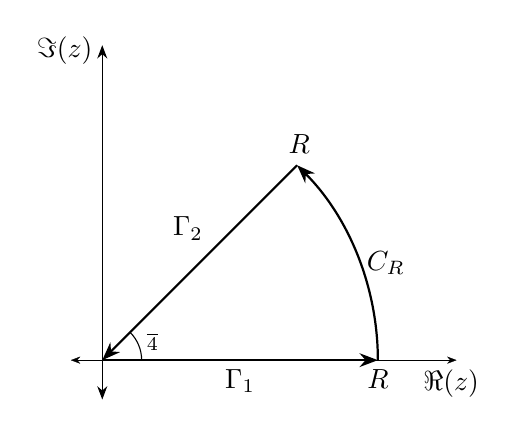
\begin{tikzpicture}[>=stealth,
                arrow style/.style={
                    postaction={decorate},
                    decoration={markings, mark=at position 0.5 with {\arrow[scale=1]{Stealth}}}
            }]

            \draw[-{Stealth}, ultra thin] (0, 0) -- (4.5, 0);
            \draw[-{Stealth}, ultra thin] (0, 0) -- (-0.4, 0);
            \draw[-{Stealth}, thin] (0, 0) -- (0, 4);
            \draw[-{Stealth}, thin] (0, 0) -- (0, -0.5);
            \draw[-{Stealth}, thick] (3.5,0) arc[start angle=0, end angle=45, radius=3.5];
            \draw[thin] (0.5,0) arc[start angle=0, end angle=45, radius=0.5];
            \draw[-{Stealth}, thick] (0, 0) -- (3.5, 0);
            \draw[-{Stealth}, thick] (2.47487, 2.47487) -- (0, 0);
            \node[anchor=north, xshift=-2pt] at (4.5, 0) {\(\Re(z)\)};
            \node[anchor=east, yshift=-2pt] at (0, 4) {\(\Im(z)\)};
            \node[anchor=west] at (0.4,0.25) {\(\tfrac{\piup}{4}\)};
            \node[anchor=north] at (1.75,0) {\(\Gamma_1\)};
            \node[anchor=south east] at (1.4,1.4) {\(\Gamma_2\)};
            \node[anchor=north] at (3.6,1.5) {\(C_R\)};
            \node[anchor=north] at (3.5,0) {\(R\)};
            \node[anchor=south] at (2.5,2.5) {\(R\)};
        \end{tikzpicture}
        \caption{A wedge contour with orientation marked.}\label{fig:wedgecontour}
    \end{figure}Let \(f(z)=\ee^{\ii z^2}\). Choose the wedge contour composed of
    \begin{gather*}
        \Gamma_1=\cbraces{x\in\mathbb{R}}{0\leq x\leq R},\qquad\Gamma_2=\cbraces{r\ee^{\ii\frac{\piup}{4}}}{0\leq r\leq R},\\
        C_R=\cbraces{R\ee^{\ii\theta}}{0\leq\theta\leq\frac{\piup}{4}}
    \end{gather*}
    as in \cref{fig:wedgecontour}. By the Cauchy--Goursat Theorem (\cref{thm:cauchygoursattheorem}), we have that
    \begin{equation}
        \int_{\Gamma_1}f(z)\ddz+\int_{\Gamma_2}f(z)\ddz+\int_{C_R}f(z)\ddz=0.\label{eq:fresnelwedgecontourintegral}
    \end{equation} The third integral can be written as \[\int_{C_R}f(z)\ddz=R\ii\int_0^{\frac{\piup}{4}}\exp[\ii{\qty(R\ee^{\ii\theta})}^2]\ee^{\ii\theta}\dd{\theta}.\]
    Using the fact that \(\frac{4}{\piup}\theta<\sin(2\theta)\) on the integration range, it can be bounded as
    \begin{align*}
        \abs{\int_{C_R}f(z)\ddz} & \leq R{\int_0^{\frac{\piup}{4}}\ee^{-R^2\sin(2\theta)}\dd{\theta}}<R\int_0^{\frac{\piup}{4}}\ee^{-\frac{4}{\piup}R^2\theta}\dd{\theta} \\
        & =-\frac{\piup}{4R}\eval{\ee^{-\frac{4}{\piup}R^2\theta}}_0^{\frac{\piup}{4}}=\frac{\piup}{4R}\qty(1-\ee^{-R^2}).
    \end{align*}
    As \(R\to\infty\), this integral tends to 0. Let \(z=r\ee^{\ii\frac{\piup}{4}}\) on \(\Gamma_2\). Then, we have \[\lim_{R\to\infty}\int_{\Gamma_2}f(z)\ddz=\int_\infty^0\exp[\ii\qty(r\ee^{\ii\frac{\piup}{4}})^2]\ee^{\ii\frac{\piup}{4}}\dd{r}=\ee^{\ii\frac{\piup}{4}}\int_\infty^0\exp(-r^2)\dd{r}.\]
    From \cref{eq:fresnelwedgecontourintegral}, we have that \[\int_0^\infty \ee^{\ii r^2}\dd{r}=\ee^{\ii\frac{\piup}{4}}\int_0^\infty \ee^{-r^2}\dd{r}.\] Since \(\int_0^\infty \ee^{-r^2}\dd{r}=\frac{\sqrt{\piup}}{2}\), we have \[\int_0^\infty \ee^{\ii r^2}\dd{r}=\qty(\frac{\sqrt{2}}{2}+\ii\frac{\sqrt{2}}{2})\frac{\sqrt{\piup}}{2}.\]
    Since \(\ee^{\ii r^2}=\cos(r^2)+\ii\sin(r^2)\), we have
    \begin{gather*}
        \int_0^\infty\cos(r^2)\dd{r}=\Re\qty[\int_0^\infty \ee^{\ii r^2}\dd{r}]=\frac{\sqrt{2\piup}}{4},\\
        \int_0^\infty\sin(r^2)\dd{r}=\Im\qty[\int_0^\infty \ee^{\ii r^2}\dd{r}]=\frac{\sqrt{2\piup}}{4},
    \end{gather*}
    as desired.
\end{proof}
\begin{example}
    Evaluate the integrals \(\int_0^{2\piup}\Phi(\cos\theta,\sin\theta)\dd{\theta}\), where \(\Phi(\xi,\eta)\) is a rational function of \(\xi\) and \(\eta\) that is continuous on \(\theta\in[0,2\piup]\).
\end{example}
\begin{proof}
    Let \(z=\ee^{\ii\theta}\). Consequently, we have \(\cos\theta=\frac{z+z^{-1}}{2}\), \(\sin\theta=\frac{z-z^{-1}}{2\ii}\), and \(\ddz=\ii\ee^{\ii\theta}\dd{\theta}\), implying that \(\dd{\theta}=\frac{\ddz}{\ii z}\). Therefore, by the Residue Theorem (\cref{thm:residuethm}), letting \(f(z)=\frac{1}{\ii z}\Phi\qty(\frac{z+z^{-1}}{2},\frac{z-z^{-1}}{2\ii})\), we have \[\int_0^{2\piup}\Phi(\cos\theta,\sin\theta)\dd{\theta}=\oint_{\partial\mathbb{D}}f(z)\ddz=2\piup\ii\sum_{k=1}^n\residue_{z=z_k}f(z),\]
    where \(z_k\) where \(k=1,\ldots,n\) are the isolated singularities of \(f\) in \(\mathbb{D}\).
\end{proof}
\begin{example}
    Evaluate \(I=\int_0^\infty\frac{x^\alpha}{1+x^\beta}\ddx\), where \(0<\alpha+1<\beta\).
\end{example}
\begin{proof}
    Let \(f(z)=\frac{z^\alpha}{1+z^\beta}\) and let \(-\piup<\Arg(z)\leq \piup\) in the principal branches of \(z^\alpha=\ee^{\alpha\Log(z)}\) and \(z^\beta=\ee^{\beta\Log(z)}\). Then except for at the zeros of \(1+z^\beta\), \(f\) is holomorphic.

    \begin{figure}
        \centering
        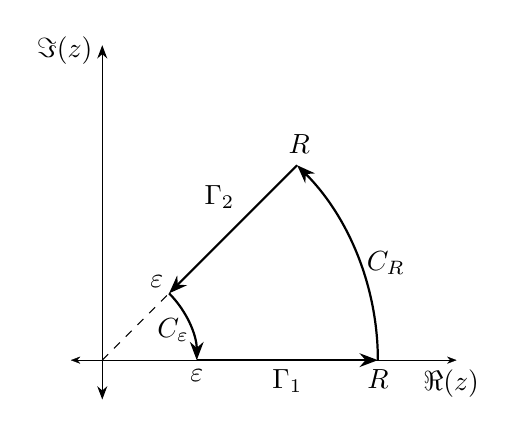
\begin{tikzpicture}[>=stealth,
                arrow style/.style={
                    postaction={decorate},
                    decoration={markings, mark=at position 0.5 with {\arrow[scale=1]{Stealth}}}
            }]

            \draw[-{Stealth}, ultra thin] (0, 0) -- (4.5, 0);
            \draw[-{Stealth}, ultra thin] (0, 0) -- (-0.4, 0);
            \draw[-{Stealth}, thin] (0, 0) -- (0, 4);
            \draw[-{Stealth}, thin] (0, 0) -- (0, -0.5);
            \draw[thin, dashed] (0, 0) -- (0.8485, 0.8485);
            \draw[-{Stealth}, thick] (3.5,0) arc[start angle=0, end angle=45, radius=3.5];
            \draw[-{Stealth}, thick] (0.8485, 0.8485) arc[start angle=45, end angle=0, radius=1.2];
            \draw[-{Stealth}, thick] (1.2, 0) -- (3.5, 0);
            \draw[-{Stealth}, thick] (2.47487, 2.47487) -- (0.8485,0.8485);
            \node[anchor=north, xshift=-2pt] at (4.5, 0) {\(\Re(z)\)};
            \node[anchor=east, yshift=-2pt] at (0, 4) {\(\Im(z)\)};
            \node[anchor=north] at (2.35,0) {\(\Gamma_1\)};
            \node[anchor=south east] at (1.8, 1.8) {\(\Gamma_2\)};
            \node[anchor=north] at (3.6,1.5) {\(C_R\)};
            \node[anchor=north] at (0.9,0.65) {\(C_\varepsilon\)};
            \node[anchor=north] at (3.5,0) {\(R\)};
            \node[anchor=north] at (1.2,0) {\(\varepsilon\)};
            \node[anchor=south] at (2.5,2.5) {\(R\)};
            \node[anchor=south east] at (0.9,0.8) {\(\varepsilon\)};
        \end{tikzpicture}
        \caption{An indented wedge contour with orientation marked.}\label{fig:indentedwedgecontour}
    \end{figure}The solutions to \(z^\beta=-1\) are \(z=\exp(\ii\frac{\piup}{\beta}+2\ii k\frac{\piup}{\beta})\). Choose an indented wedge contour (as there is a logarithmic branch point singularity at the origin) with an angle of \(\frac{2\piup}{\beta}\) (as in \cref{fig:wedgecontour}). The only singularity it encloses is \(\exp(\ii\frac{\piup}{\beta})\). Since it is a simple zero of \(\frac{1}{f}\), this singularity is a simple pole.

    The contour is the union of the following curves:\
    \begin{gather*}
        \Gamma_1=\cbraces{x\in\mathbb{R}}{\varepsilon\leq x\leq R},\qquad\Gamma_2=\cbraces{r\exp(\ii\frac{2\piup}{\beta})}{\varepsilon\leq r\leq R},\\
        C_R=\cbraces{R\ee^{\ii\theta}}{0\leq\theta\leq \frac{2\piup}{\beta}},\qquad C_\varepsilon=\cbraces{\varepsilon\ee^{\ii\theta}}{0\leq\theta\leq \frac{2\piup}{\beta}}
    \end{gather*}
    where \(R>1\) and \(0<\varepsilon<1\). By the Residue Theorem (\cref{thm:residuethm}), we get that \[\lim_{\varepsilon\to 0}\lim_{R\to\infty}\qty(\int_{\Gamma_1}+\int_{\Gamma_2}+\int_{C_R}+\int_{C_\varepsilon})f(z)\ddz=2\piup\ii\Res[f,\exp(\ii\frac{\piup}{\beta})].\]
    By \cref{eq:residueatpole}, it follows that
    \begin{align*}
        \residue\qty[f,\exp(\ii\frac{\piup}{\beta})] & =\lim_{z\to\exp(\ii\frac{\piup}{\beta})}\flatfrac{\qty[z-\exp(\ii\frac{\piup}{\beta})]}{\qty[\frac{1+z^\beta}{z^\alpha}]} \\
        & =\lim_{z\to\exp(\ii\frac{\piup}{\beta})}{\dv{z}(z^{-\alpha}+z^{\beta-\alpha})}^{-1}                                     \\
        & =\lim_{z\to\exp(\ii\frac{\piup}{\beta})}\frac{z^{\alpha+1}}{(\beta-\alpha)z^{\beta}-\alpha}                             \\
        & =-\frac{1}{\beta}\exp(\ii\frac{\piup}{\beta}(\alpha+1)).
    \end{align*}
    We can write the integral on \(\Gamma_2\) in terms of \(I\):
    \begin{align*}
        \lim_{\substack{R\to\infty\\\varepsilon\to 0}}\int_{\Gamma_2}f(z)\ddz & =\lim_{\substack{R\to\infty\\\varepsilon\to 0}}\int_R^0 f\qty[r\exp(\ii\frac{2\piup}{\beta})]\exp(\ii\frac{2\piup}{\beta})\dd{r}   \\
        & =-\exp[\ii\frac{2\piup}{\beta}(1+\alpha)]\int_0^\infty\frac{r^\alpha}{1+r^\beta}\dd{r}.
    \end{align*}
    We also have \[\int_{C_R}f(z)\ddz=R\ii\int_{0}^{\frac{2\piup}{\beta}}f\qty(R\ee^{\ii\theta})\ee^{\ii\theta}\dd{\theta}=\ii\int_0^{\frac{2\piup}{\beta}}\frac{R^{\alpha+1}}{1+R^\beta \ee^{\ii\beta\theta}}\exp[\ii\theta(1+\alpha)]\dd{\theta}.\] It can also be shown that the integral is bounded by a vanishing function as \(R\to\infty\):
    \[\abs{\int_0^{\frac{2\piup}{\beta}}\frac{R^{\alpha+1}}{1+R^\beta \ee^{\ii\beta\theta}}\exp[\ii\theta(1+\alpha)]\dd{\theta}}\leq\int_0^{\frac{2\piup}{\beta}}\frac{R^{\alpha+1}}{R^\beta-1}\dd{\theta}=\frac{2\piup}{\beta}\frac{R^{\alpha+1}}{R^\beta-1}\to 0.\]
    Similarly, as \(\varepsilon\to 0\), \[\abs{\int_{C_\varepsilon}f(z)\ddz}\leq\varepsilon\int_0^{\frac{2\piup}{\beta}}\abs{f\qty(\varepsilon\ee^{\ii\theta})}\dd{\theta}=\int_0^{\frac{2\piup}{\beta}}\frac{\varepsilon^{\alpha+1}}{1-\varepsilon^\beta}\dd{\theta}=\frac{2\piup}{\beta}\frac{\varepsilon^{\alpha+1}}{1-\varepsilon^{\beta}}\to 0.\]
    By letting \(R\to\infty\) and \(\varepsilon\to 0\), we have \[\qty[1-\exp(\ii\frac{2\piup}{\beta}(1+\alpha))]I=-\frac{2\piup\ii}{\beta}\exp(\ii\frac{\piup}{\beta}(\alpha+1)).\]
    It follows that \[I=\frac{2\piup\ii}{\beta}\brackets{\exp(\ii\frac{\piup}{\beta}(\alpha+1))-\exp(-\ii\frac{\piup}{\beta}(\alpha+1))}^{-1}=\frac{\piup}{\beta}\csc(\frac{\piup}{\beta}(\alpha+1)).\qedhere\]
\end{proof}
\begin{example}
    Prove that the Fourier transform of \(\sech(\piup x)\) is itself, or that \[I(\xi)=\int_{-\infty}^\infty\exp(-2\piup \ii x\xi)\sech(\piup x)\ddx=\sech(\piup\xi).\]
\end{example}
\begin{proof}
    Fix \(\xi\in\mathbb{R}\) and let \(f(z)=\frac{\exp(-2\piup \ii z\xi)}{\cosh(\piup z)}\). Its poles in \(\mathbb{C}\) occur when \(\ee^{\piup z}+\ee^{-\piup z}=0\), or equivalently, when \(z=\ii\qty(n+\frac{1}{2})\), where \(n\in\mathbb{Z}\).

    \begin{figure}
        \centering
        \begin{tikzpicture}[>=stealth,
                arrow style/.style={
                    postaction={decorate},
                    decoration={markings, mark=at position 0.5 with {\arrow[scale=1]{Stealth}}}
            }]

            \draw[-{Stealth}, ultra thin] (0, 0) -- (5, 0);
            \draw[-{Stealth}, ultra thin] (0, 0) -- (-5, 0);
            \draw[-{Stealth}, thin] (0, 0) -- (0, 3);
            \draw[-{Stealth}, thin] (0, 0) -- (0, -0.5);
            \draw[-{Stealth}, thick] (-3, 0) -- (0, 0);
            \draw[-{Stealth}, thick] (0, 0) -- (3, 0);
            \draw[-{Stealth}, thick] (3, 0) -- (3, 2);
            \draw[-{Stealth}, thick] (3, 2) -- (0, 2);
            \draw[-{Stealth}, thick] (0, 2) -- (-3, 2);
            \draw[-{Stealth}, thick] (-3, 2) -- (-3, 0);
            \node[anchor=north, xshift=-2pt] at (5, 0) {\(\Re(z)\)};
            \node[anchor=east, yshift=-2pt] at (0, 3) {\(\Im(z)\)};
            \node[anchor=north] at (3,0) {\(R\)};
            \node[anchor=north] at (-3,0) {\(-R\)};
            \node[anchor=south east] at (0,2) {\(\ii\)};
        \end{tikzpicture}
        \caption{A rectangular contour with orientation marked.}\label{fig:rectangularcontour}
    \end{figure}Since \[\cosh(\piup(z+\ii))=-\cosh(\piup z),\qquad\exp(-2\piup\ii(z+\ii)\xi)=\exp(2\piup\xi)\exp(-2\piup \ii z\xi),\] we have that \(f(z)\) is a constant multiple of \(f(z+\ii)\). In particular, \(f(z+\ii)=-\exp(2\piup\xi)f(z)\). Therefore, we can use a rectangular contour as shown in \cref{fig:rectangularcontour}. Let the sides be denoted by
    \begin{gather*}
        \overleftarrow{\Gamma}=\cbraces{x+\ii}{-R\leq x\leq R,x\in\mathbb{R}},\qquad\overrightarrow{\Gamma}x=\cbraces{x\in\mathbb{R}}{-R\leq x\leq R}\\
        \overset{\downarrow}{\Gamma}=\cbraces{-R+\ii y}{y\in[0,1]},\qquad\overset{\uparrow}{\Gamma}=\cbraces{R+\ii y}{y\in[0,1]}.
    \end{gather*}
    The only enclosed singularity is a simple pole at \(z=\frac{\ii}{2}\) (simple by evaluation of the Taylor expansion of the denominator). By the Residue Theorem (\cref{thm:residuethm}), we get that
    \begin{equation}
        \qty(\int_{\overrightarrow{\Gamma}}+\int_{\overset{\uparrow}{\Gamma}}+\int_{\overleftarrow{\Gamma}}+\int_{\overset{\downarrow}{\Gamma}})f(z)\ddz=2\piup\ii\Res(f,\frac{\ii}{2}).\label{eq:fouriertransformofsechpix_rectangularcontourintegral}
    \end{equation}
    By \cref{eq:residueatpole}, we have
    \begin{align*}
        \Res(f,\frac{\ii}{2}) & =\lim_{z\to\frac{\ii}{2}}\qty(z-\frac{\ii}{2})\frac{\exp(-2\piup \ii z\xi)}{\cosh(\piup z)}      \\
        & =\lim_{z\to\frac{\ii}{2}}\dv{z}(\frac{\cosh(\piup z)}{\exp(-2\piup \ii z\xi)})^{-1}              \\
        & =\lim_{z\to\frac{\ii}{2}}\frac{\exp(-2\piup \ii z\xi)}{\piup\sinh(\piup z)+2\piup\ii\xi\cosh(\piup z)} \\
        & =\frac{\exp(\piup\xi)}{\piup \ii}.
    \end{align*}
    The sum of the horizontal line integrals is equal to
    \begin{align*}
        \int_{-R}^R f(z)\ddz+\int_R^{-R}f(z+\ii)\ddz & =\int_{-R}^R f(z)\ddz-\int_R^{-R}\ee^{2\piup\xi}f(z)\ddz \\
        & =\qty(1+\ee^{2\piup\xi})\int_{-R}^R f(z)\ddz.
    \end{align*} As \(R\to\infty\), we have \(\int_{\overrightarrow{\Gamma}}f(z)\ddz+\int_{\overleftarrow{\Gamma}}f(z)\ddz\to\qty(1+\ee^{2\piup\xi})I(\xi)\).
    The remaining two integrals can be written as
    \begin{align*}
        \int_{\overset{\uparrow}{\Gamma}}f(z)\ddz=\int_0^1 \frac{\exp(-2\piup\ii(R+\ii z)\xi)}{\cosh(\piup(R+\ii z))}\ddz \\
        \int_{\overset{\downarrow}{\Gamma}}f(z)\ddz=\int_1^0 \frac{\exp(2\piup\ii(R-\ii z)\xi)}{\cosh(\piup(-R+\ii z))}\ddz.
    \end{align*}
    They can be bounded with
    \begin{align*}
        \abs{\int_0^1 \frac{\exp(-2\piup\ii(R+\ii z)\xi)}{\cosh(\piup(R+\ii z))}\ddz} & \leq 2\int_0^1\frac{\exp(2\piup z\xi)}{\abs{\ee^{\piup R}\ee^{\piup \ii z}+\ee^{-\piup R}\ee^{-\piup \ii z}}}\ddz \\
        & \leq2\int_0^1\frac{\exp(2\piup z\xi)}{\abs{\ee^{\piup R}-\ee^{-\piup R}}}\ddz
    \end{align*} and
    \begin{align*}
        \abs{\int_1^0 \frac{\exp(2\piup\ii(R-\ii z)\xi)}{\cosh(\piup(-R+\ii z))}\ddz} & \leq 2\int_0^1\frac{\exp(2\piup z\xi)}{\abs{\ee^{-\piup R}\ee^{\piup \ii z}+\ee^{\piup R}\ee^{-\piup \ii z}}}\ddz \\
        & \leq2\int_0^1\frac{\exp(2\piup z\xi)}{\abs{\ee^{\piup R}-\ee^{-\piup R}}}\ddz
    \end{align*}
    Since the integrands are continuous and uniformly convergent to \(0\) with respect to \(z\), we have \[\int_{\overset{\uparrow}{\Gamma}}f(z)\ddz+\int_{\overset{\downarrow}{\Gamma}}f(z)\ddz\to 0\] as \(R\to\infty\). By rearrangement of \cref{eq:fouriertransformofsechpix_rectangularcontourintegral}, \[I(\xi)\qty(1+\ee^{2\piup\xi})=2\exp(\piup\xi),\]
    or that \[I(\xi)=\frac{2}{\ee^{-\piup\xi}+\ee^{\piup\xi}}=\sech(\piup\xi),\] which proves the result.
\end{proof}
Contour integration provides a powerful method for evaluating real improper integrals by leveraging the Residue Theorem (\cref{thm:residuethm}). The primary challenge often lies in constructing a suitable contour in the complex plane that encloses the relevant singularities of the integrand \(f\) while ensuring that the contribution from the contributions from the remaining segments of the contour either vanishes or can be calculated with ease.

If the function \(f\) is even and integrated on a domain such as \(\mathbb{R}_{\geq0}\), then the integral can be extended to the entire real axis. If \(f\) decays sufficiently rapidly in the upper half plane \(\mathbb{H}^+\), a semicircular contour is generally preferable, as illustrated in \cref{fig:semicircularcontour}. In the presence of singularities on the contour itself, we can insert arc indentations around them, as shown in \cref{fig:indentedsemicircularcontour}.

If \(f(z)\) is a constant multiple of \(f(z+\ii y)\) for some \(y\in\mathbb{R}\), it is a strong indication to use a rectangular contour. If \(f(z)\) is a constant multiple of \(f\qty(z\ee^{\ii\tau})\) for some \(\tau\in\mathbb{R}\), a wedge-shaped contour is an appropriate choice.

In the case that there are indentations along the contour, we have
\begin{theorem}\label{thm:residueoverarc}
    Let \(\lambda>0\) and let \(a\in\mathbb{C}\). Suppose \(f(z)\) is a holomorphic function on \(D^*(a,\lambda)\) with a simple pole at \(z=a\in U\). Let \(0<\varepsilon<\lambda\) and define \(\gamma_\varepsilon\subseteq\partial D(a, \varepsilon)\) be a counterclockwise-oriented, connected arc subtending an angle \(\vartheta\). Then,
    \[\lim_{\varepsilon\to 0}\int_{\gamma_\varepsilon}f(z)\ddz=\ii\vartheta\cdot\residue_{z=a}f(z).\]
\end{theorem}
\begin{proof}
    Parameterize \(\gamma_\varepsilon\) with \(z=a+\varepsilon \ee^{\ii\theta}\), where \(\theta\in[\alpha,\beta]\) and \(\beta-\alpha=\vartheta\). Then,
    \[\int_{\gamma_\varepsilon} f(z)\ddz = \int_\alpha^\beta f\qty(a+\varepsilon \ee^{\ii\theta}) \dv{z}{\theta}\dd{\theta}=\varepsilon \ii \int_\alpha^\beta f\qty(a+\varepsilon \ee^{\ii\theta})\ee^{\ii\theta}\dd{\theta}.\]
    Since \(f\) has a simple pole at \(z=a\), we can write a Laurent expansion around \(a\) as
    \[f(z)=\frac{c_{-1}}{z-a}+\varphi(z),\]
    where \(\varphi(z)\) is holomorphic in a neighborhood of \(a\) and \(c_{-1}=\residue_{z=a}f(z)\).

    Then for \(z=a+\varepsilon \ee^{\ii\theta}\),
    \[f\qty(a+\varepsilon \ee^{\ii\theta})=\frac{c_{-1}}{\varepsilon \ee^{\ii\theta}}+\varphi\qty(a+\varepsilon \ee^{\ii\theta}).\]
    So,
    \begin{align*}
        \int_{\gamma_\varepsilon}f(z)\ddz
        & = \varepsilon \ii\int_\alpha^\beta \qty(\frac{c_{-1}}{\varepsilon\ee^{\ii\theta}}+\varphi\qty(a+\varepsilon\ee^{\ii\theta}))\ee^{\ii\theta}\dd{\theta} \\
        & = \ii c_{-1}\int_\alpha^\beta\dd{\theta}+\varepsilon \ii\int_\alpha^\beta\varphi\qty(a+\varepsilon \ee^{\ii\theta})\ee^{\ii\theta}\dd{\theta}          \\
        & = \ii c_{-1}\vartheta+\varepsilon \ii\int_\alpha^\beta\varphi\qty(a+\varepsilon\ee^{\ii\theta})\ee^{\ii\theta}\dd{\theta}.
    \end{align*}
    Let \(\varepsilon<\frac{\lambda}{2}\). Since \(\varphi\) is continuous on the disk \(\overline{D\qty(a,\frac{\lambda}{2})}\), it is bounded. Therefore, letting \(\varepsilon\to0\), we have
    \[\lim_{\varepsilon\to 0} \varepsilon \ii \int_\alpha^\beta\varphi\qty(a+\varepsilon\ee^{\ii\theta})\ee^{\ii\theta}\dd{\theta}=\lim_{\varepsilon\to 0}\varepsilon \ii\int_\alpha^\beta\varphi(a)\ee^{\ii\theta}\dd{\theta}=0.\]
    Therefore,
    \[\lim_{\varepsilon \to 0}\int_{\gamma_\varepsilon}f(z)\ddz=\ii\vartheta\residue_{z=a}f(z).\qedhere\]
\end{proof}
In the case that a branch point singularity is present on the contour, we may attempt to rewrite the function in a way such that the branch point is irrelevant. Otherwise, there are two types of ``keyhole contours'' that can be used to avoid the branch cut.
\begin{example}\label{ex:branchpointpoleconcurrenceintegral}
    Evaluate \(I=\int_0^\infty\frac{\log(x^2+1)}{x^2+1}\ddx\).
\end{example}
\begin{proof}
    Notice that the integrand itself has branch points at \(z=\pm\ii\) coinciding with the poles from the denominator. We can rewrite the integral as
    \begin{align}
        I&=\frac{1}{2}\int_{-\infty}^\infty\frac{\log\qty(x^2+1)}{x^2+1}=\int_{-\infty}^\infty\frac{\log\sqrt{(x+i)(x-i)}}{x^2+1}\nonumber\\
        &=\int_{-\infty}^\infty\frac{\log\abs{x\pm i}}{x^2+1}=\Re\int_{-\infty}^\infty\frac{\log\qty(x+i)}{x^2+1}.\label{eq:branchpointpoleconcurrenceintegral_rewrite}
    \end{align}
    Let \(\gamma=\Gamma\cup C_{R}\), where concretely, \[\Gamma=\cbraces{x\in\mathbb{R}}{-R\leq x\leq R},\qquad C_{R}=\cbraces{R\ee^{\ii\theta}}{0\leq\theta\leq\piup}\] and \(R>2\), and let \(f(z)=\frac{\Log(z+\ii)}{z^2+1}\), where the branch for \(\Log\) is chosen to satisfy \([0,\piup]\subset\Im\log\qty(\mathbb{C}^*)\), such as the principal branch. The only singularity of \(f\) in the upper half plane is a simple pole at \(z=\ii\). By the Residue Theorem (\cref{thm:residuethm}), we have \[\lim_{R\to\infty}\oint_{\gamma}f(z)\ddz=\lim_{R\to\infty}\qty(\int_\Gamma+\int_{C_R})f(z)\ddz=2\piup\ii\residue_{z=\ii}f(z).\]
    By \cref{eq:residueatpole}, we have \[\residue_{z=\ii}f(z)=\lim_{z\to\ii}\qty(z-\ii)\frac{\log(z+\ii)}{z^2+1}=\lim_{z\to\ii}\frac{\log(z+\ii)}{z+\ii}=\frac{\log(2\ii)}{2\ii}=\frac{\piup}{4}-\ii\frac{\log(2)}{2}.\]
    Additionally, for \(z\in C_R\), since as \(R\to\infty\), \(\abs{f(z)}=\abs{\frac{\Log(z+i)}{z^2+1}}\leq\frac{\abs{\log\abs{z+i}}+\piup}{R^2-1}\leq\frac{\log\abs{R+1}+\piup}{R^2-1}<\frac{R+1+\piup}{R^2-1}\to 0\) by virtue of \(R>2\), it follows that \(\int_{C_R}f(z)\ddz\to 0\).

    Since \(\lim_{R\to\infty}\int_\Gamma f(z)\ddz=\int_{-\infty}^\infty f(z)\ddz\) and \[\int_{-\infty}^\infty f(z)\ddz=\frac{\piup^2\ii}{2}+\piup\log(2),\] by \cref{eq:branchpointpoleconcurrenceintegral_rewrite}, we have \(I=\Re\int_{-\infty}^\infty f(z)\ddz=\piup\log(2)\).
\end{proof}
\section{Analytic Continuation}\label{sec:analyticcontinuation}
\subsection{Analytic Function Elements}
\begin{definition}\label{def:analyticelement}
    An \textscsl{analytic function element} is a pair \((f,U)\), where \(U\subseteq\mathbb{C}\) is an open disk and \(f\) is a holomorphic function on \(U\).
\end{definition}
Analytic elements serve as local representations of analytic functions. The process of extending these elements is formalized through \textscsl{analytic continuation}, previously introduced in \cref{def:analyticcontinuation}.

By the Identity Theorem (\cref{thm:identity}), such continuations are unique; if \(\qty(f_1,U_1)\) and \(\qty(f_2,U_2)\) are analytic elements with \(U_1\cap U_2 \neq \emptyset\), and \(f_1\equiv f_2\) on \(U_1\cap U_2\), then they are \textscsl{direct analytic continuations} of each other. The combined function:
\[\widetilde{f}(z)=
    \begin{cases}
        f_1(z) &\qif* z\in U_1               \\
        f_2(z) &\qif* z\in U_2 \setminus U_1
\end{cases}\] is holomorphic on \(U_1\cup U_2\).

The most straightforward method of the derivation of analytic continuations uses power series. Let \(f(z)=\sum_{n=0}^{\infty}c_n\qty(z-z_0)^n\) have radius of convergence \(R>0\) (by \cref{thm:abelradius}). For \(z_1\in D\qty(z_0,R)\), we can expand \(f\) at \(z_1\):
\[f(z)=\sum_{k=0}^\infty\frac{f^{(k)}\qty(z_1)}{k!}\qty(z-z_1)^k.\]
Let \(\rho\) be the radius of convergence of this series. Then:
\[\rho\geq R-\abs{z_1-z_0}.\]
If \(\rho>R-\abs{z_1-z_0}\), then \(f\) extends analytically to \(D\qty(z_0,R) \cup D(z_1,\rho)\). In the case that \(\rho=R-\abs{z_1-z_0}\), the disks \(D\qty(z_0,R)\) and \(D\qty(z_1,\rho)\) are tangent at a point \(\zeta_0\). Here, \(\zeta_0\) is a \textscsl{singularity}, and \(f\) cannot be continued beyond \(\zeta_0\).
\begin{theorem}\label{thm:boundarysingularity}
    Let \(f(z)=\sum_{n=0}^{\infty}c_n{\qty(z-z_0)}^n\) have radius of convergence \(R>0\). Then \(\partial D\qty(z_0,R)\) contains at least one singularity of \(f\).
\end{theorem}
\begin{proof}
    Assume \(f\) can be analytically continued from every \(\zeta\in\partial D\qty(z_0,R)\). Then for each \(\zeta\), there exists \(r_\zeta>0\) and a holomorphic \(f_\zeta\) on \(D\qty(\zeta,r_\zeta)\) agreeing with \(f\) on \(D\qty(\zeta,r_\zeta) \cap D\qty(z_0,R)\).

    The disks \(\cbraces{D\qty(\zeta,r_\zeta)}_{\zeta \in\partial D\qty(z_0,R)}\) cover \(\partial D\qty(z_0,R)\). Then from compactness and the Heine--Borel Theorem (\cref{thm:heineborel}), the cover of disks admits a finite subcover \(\qty{D\qty(\zeta_k,r_k)}_{k=1}^n\). Hence, \(\exists\rho>0\) such that \(A=\cbraces{z}{R-\rho\leq\abs{z-z_0}\leq R+\rho}\subset V\), where we let \(V=\bigcup_{k=1}^n D\qty(\zeta_k,r_k)\).

    Define \(\Phi:V\to\mathbb{C}\) by \(\Phi(z)=f_{\zeta_k}(z)\) if \(z\in D\qty(\zeta_k,r_k)\). This is well-defined: If \(z\in D\qty(\zeta_i,r_i)\cap D\qty(\zeta_j,r_j)\), then \(D\qty(\zeta_i,r_i)\cap D\qty(\zeta_j,r_j) \cap D\qty(z_0,R)\neq\emptyset\), and \(f_{\zeta_i}=f_{\zeta_j}=f\) there. By the Identity Theorem (\cref{thm:identity}), \(f_{\zeta_i}\equiv f_{\zeta_j}\) on \(D\qty(\zeta_i,r_i)\cap D\qty(\zeta_j,r_j)\).

    Since \(\Phi\) is holomorphic on \(V\) and agrees with \(f\) on \(D\qty(z_0,R)\cap V\), the function:
    \[\widetilde{f}(z)=
        \begin{cases}
            f(z)    &\qif* z\in D\qty(z_0,R) \\
            \Phi(z) &\qif* z\in V
    \end{cases}\]
    is holomorphic on \(D\qty(z_0,R)\cup V\supseteq D(z_0, R+\rho)\), contradicting the maximality of \(R\).
\end{proof}
\begin{definition}\label{def:maximalanalyticcontinuation}
    A \textscsl{maximal analytic continuation} \(\qty{\qty(f,U)}\) of an analytic function element \(\qty(\widetilde{f},\widetilde{U})\) is obtained by all possible succesive analytic continuations of \(\qty(\widetilde{f},\widetilde{U})\). The union of every \(U\) is known as the \textscsl{domain of holomorphy} of \(\widetilde{f}\). The boundary set \(\partial U\) is known as a \textscsl{natural boundary}. The continuation defines a function \(f\), known a \textscsl{global analytic function}, which can be multi-valued.
\end{definition}
\begin{example}\label{ex:factoriallacunaryseries}
    The series \(f(z)=\sum_{n=0}^{\infty}z^{n!}\) has \(\mathbb{D}\) as its disk of convergence, and every point on \(\partial\mathbb{D}\) is a singularity.
\end{example}
\begin{proof}
    By Cauchy--Hadamard (\cref{thm:cauchyhadamard}), \(\varlimsup_{n\to\infty}\sqrt[n]{\abs{c_n}}=1\) since \(c_n=1\) if \(n=k!\) and \(0\) otherwise. Thus, \(R=1\).

    Fix \(\zeta\in\partial\mathbb{D}\). Suppose \(f\) extends analytically to a disk \(D(\zeta,\delta)\). Since \(\exp(2\piup\ii\mathbb{Q})\) is dense in \(\partial\mathbb{D}\), there exists \(\zeta'=\exp(2\piup\ii\frac{p}{q})\in D(\zeta,\delta)\cap\partial\mathbb{D}\) for coprime integers \(p,q\). The extension \(g\) of \(f\) to \(D(\zeta, \delta)\) would satisfy:
    \[\lim_{r\to1^{-}}f(r\zeta')=g(\zeta').\]
    However, for \(0<r<1\):
    \[f(r\zeta')=\sum_{k=0}^{q-1}{\qty(r\zeta')}^{k!}+\sum_{k=q}^\infty r^{k!}\zeta'^{k!}.\]
    The second summation is unbounded since \[\sum_{k=q}^\infty r^{k!}\zeta'^{k!}=\sum_{k=q}^\infty r^{k!}>\sum_{k=q}^N r^{k!}>(N-q+1)r^{N!}\] for any integer with \(N>q\). Hence, as \(r\to1^-\), \(\sum_{k=q}^{\infty} r^{k!}\to\infty\). Hence, \(\zeta\) is a singularity.
\end{proof}
\begin{example}
    Show that \(f(z)=\sum_{n=0}^\infty z^{2^n}\) cannot be analytically continued to the outside of \(\mathbb{D}\).
\end{example}
\begin{proof}
    Trivially, at \(z=1\), the series diverges. Therefore, \(\mathbb{D}\) is its convergence disk. Observe that \(f(z)=\sum_{n=0}^\infty \qty(z^2)^{2^{n-1}}=\sum_{n=0}^\infty \qty(z^2)^{2^n}+z=f\qty(z^2)+z\). Hence, we have \[f(z)=f\qty(z^2)+z=f\qty(z^4)+z^2+z=f\qty(z^8)+z^4+z^2+z\cdots,\]
    which diverges at each \(z^2,z^4,z^8,\ldots=1\). The solutions form a dense set in \(\partial\mathbb{D}\). By the same reasoning as \cref{ex:factoriallacunaryseries}, \(f\) cannot be analytically continued to the outside of \(\mathbb{D}\).
\end{proof}
\begin{example}\label{ex:complexlogarithmanalyticcontinuation}
    Let \(\Log(z)\) denote the principal branch of \(\log(z)\), with \(-\piup<\Arg(z)\leq\piup\). The analytic function elements \[\qty(\Log,D(1,1))\qand\qty(\Log+2\piup\ii,D(1,1))\] are analytic continuations of each other.
\end{example}
\begin{example}
    Show that the analytic functions defined by the series \(f(z)=\sum_{n=0}^\infty\alpha^n z^n\) and \(\widetilde{f}(z)=\sum_{n=0}^\infty\frac{(\alpha-1)^n z^n}{{\qty(1-z)}^{n+1}}\) are analytic continuations of each other.
\end{example}
\begin{proof}
    The analytic function element \(\qty(f,D\qty(0,\abs{\frac{1}{\alpha}}))\) can be directly continued to the analytic function element \(\qty(z\mapsto\frac{1}{1-\alpha z},\mathbb{C}\setminus\qty{\frac{1}{\alpha}})\). The function element \(\qty(\widetilde{f},D\qty(0,\frac{1-z}{\alpha-1}))\) can be analytically continued to \[\qty(z\mapsto\frac{1}{(1-z)\qty(1-\frac{z\alpha-z}{1-z})},\mathbb{C}\setminus\qty{1,\frac{1}{\alpha}})=\qty(z\mapsto\frac{1}{1-\alpha z},\mathbb{C}\setminus\qty{1,\frac{1}{\alpha}}),\] which is a direction analytic continuation of \(\qty(z\mapsto\frac{1}{1-\alpha z},\mathbb{C}\setminus\qty{\frac{1}{\alpha}})\). Therefore, \(f\) and \(\widetilde{f}\) are analytic continuations of each other.
\end{proof}
In \cref{ex:complexlogarithmanalyticcontinuation}, we showed that two analytic function elements can on the same domain can be analytic continuations even if they do not agree on the entire domain. In this case, the two elements are on different branches of the function. Hence, depending on the chain of function elements chosen, we may obtain two different analytic function elements that have the same domain.

This is a common issue when it comes to the problem of analytic continuation. This question of non-ambiguity can be explained by planar topology; specifically the concept of homotopy. We will now introduce the concept of analytic continuation along a given curve.
\subsection{Analytic Continuation Along a Curve}
\begin{definition}\label{def:analyticcontinuationalongcurve}
    Let \(\gamma:[0,1]\to\mathbb{C}\) be a (non-constant) curve. Let \(U\) be a disk centered at \(\gamma(0)\) and suppose \(f: U\to\mathbb{C}\) is holomorphic. An \textscsl{analytic continuation of} \(\qty(f,U)\) \textscsl{along} \(\gamma\) is defined to be a collection of analytic functions elements \(\qty{\qty(f_t, U_t)}_{0\leq t\leq 1}\) where
    \begin{enumerate}
        \item We define \(U_0=U\) and \(f_0=f\).
        \item Each \(U_t\) (\(0\leq t\leq 1\)) is a disk centered at \(\gamma(t)\).
        \item For each \(t_0\in [0,1]\), \(\exists\delta>0\) such that \(\forall t\in[0,1]\) satisfying \(\abs{t-t_0}<\delta\), \(\gamma(t)\in U_{t_0}\) and \(f_t\equiv f_{t_0}\) on \(U_t\cap U_{t_0}\neq\emptyset\).\label{itm:analyticcontinuationalongcurve_pointwiseequivalence}
    \end{enumerate}
\end{definition}
For a fixed curve, such analytic continuations are unique in the following sense:
\begin{lemma}\label{lem:analyticcontinuationalongcurveuniqueness}
    For a fixed curve \(\gamma:[0,1]\to\mathbb{C}\), let \(f\) be holomorphic on \(U\) (a disk centered at \(\gamma(0)\)). Then any two analytic continuations \(\qty{\qty(f_t,U_t)}_{0\leq t\leq 1}\) and \(\qty{\qty(\widetilde{f}_t,\widetilde{U}_t)}_{0\leq t\leq 1}\) along \(\gamma\) satisfy \(f_1\equiv\widetilde{f}_1\) on \(U_1\cap\widetilde{U}_1\) (where \(\qty(f_1,U_1)\) and \(\qty(\widetilde{f}_t,\widetilde{U}_t)\) are the respective terminal analytic function elements).
\end{lemma}
\begin{proof}
    Let \(S\subseteq[0,1]\) be the set of all \(t_0\) such that \(\forall 0\leq t\leq t_0\), \(f_t\equiv \widetilde{f}_t\) on \(U_t\cap\widetilde{U}_t\) (this intersection is nonempty since \(\gamma(t)\in U_t,\widetilde{U}_t\)). Since \(0\in S\), it follows that \(S\) is nonempty.

    Obviously, \(S\) is a connected set. Indeed, for any \(t_0\) in \(S\), any \(0\leq t<t_0\) also lies in \(S\) by definition.

    Let \(t_\infty=\sup(S)\), and choose an increasing sequence \(\qty{t_n}_{n\in\mathbb{N}}\subseteq S\) that converges to \(t_\infty\). By~\ref{itm:analyticcontinuationalongcurve_pointwiseequivalence} of \cref{def:analyticcontinuationalongcurve}, \(\exists\delta>0\) such that \(\forall n\in\mathbb{N}\) satisfying \(\abs{t_\infty-t_n}<\delta\), \[f_{t_n}\equiv f_{t_\infty}\qq{on} U_{t_n}\cap U_{t_\infty}.\] Similarly, \(\exists\widetilde{\delta}>0\) such that \(\forall n\in\mathbb{N}\) satisfying \(\abs{t_\infty-t_n}<\widetilde{\delta}\), \[\widetilde{f}_{t_n}\equiv\widetilde{f}_{t_\infty}\qq{on}\widetilde{U}_{t_n}\cap\widetilde{U}_{t_\infty}.\]
    Choose \(n\) arbitrarily to satisfy \(\abs{t_\infty-t_n}<\min\qty(\delta,\widetilde{\delta})\). By definition, \[\gamma\qty(t_n)\in U_{t_\infty}\qand \gamma\qty(t_n)\in\widetilde{U}_{t_\infty}.\] Hence, \(\widetilde{U}_{t_\infty}\cap U_{t_\infty}\cap \widetilde{U}_{t_n}\cap U_{t_n}\neq\emptyset\). Since \(t_n\in S\), it follows that \(\widetilde{f}_{t_n}\equiv f_{t_n}\) on \(\widetilde{U}_{t_n}\cap U_{t_n}\). Thus, \[f_{t_\infty}\equiv\widetilde{f}_{t_\infty}\qq{on}\widetilde{U}_{t_\infty}\cap U_{t_\infty}\cap \widetilde{U}_{t_n}\cap U_{t_n}.\] By the Identity Theorem (\cref{thm:identity}), this equality holds on the entire intersection \(\widetilde{U}_{t_\infty}\cap U_{t_\infty}\). It follows that \(t_\infty\in S\) and thus \(S\) is closed.

    Let \(\widetilde{S}=[0,1]\setminus S\), and assume that it is nonempty (if not, our result is proven). Suppose \(\qty{t_n}_{n\in\mathbb{N}}\subset\widetilde{S}\) is an arbitrary sequence that converges to \(t_\infty\). For each \(n\in\mathbb{N}\), since \(t_n\notin S\), by definition, there exists \(0\leq s_n\leq t_n\) such that \(f_{s_n}\not\equiv \widetilde{f}_{s_n}\) on \(U_{s_n}\cap\widetilde{U}_{s_n}\) (otherwise \(t_n\in S\) would be satisfied).

    By the Bolzano--Weierstrass Theorem (\cref{thm:bolzanoweierstrass}), the sequence \(\qty{s_n}_{n\in\mathbb{N}}\) has a convergent subsequence \(\qty{s_{n_k}}_{k\in\mathbb{N}}\) that converges to \(s_\infty\). Since \(t_{n_k}\to t_\infty\) and \(s_{n_k}\leq t_{n_k}\) for all \(k\), it follows that \(s_\infty\leq t_\infty\). By definition, there exists \(\delta>0\) (choose it to be the minimum of the two \(\delta\) values, similar to in the previous section) such that \(\forall t\in[0,1]\) satisfying \(\abs{t-s_\infty}<\delta\), \(f_t\equiv f_{s_\infty}\) and \(\widetilde{f}_t\equiv \widetilde{f}_{s_\infty}\) on \(U_t\cap U_{s_\infty}\) and on \(\widetilde{U}_t\cap \widetilde{U}_{s_\infty}\) respectively, and \(\gamma\qty(t)\in U_{s_\infty}\cap \widetilde{U}_{s_\infty}\).

    Since \(s_{n_k}\to s_\infty\), we have \(\abs{s_{n_k}-s_\infty}<\delta\) for sufficiently large \(k\). Thus, \(f_{s_{n_k}}\equiv f_{s_\infty}\) and \(\widetilde{f}_{s_{n_k}}\equiv \widetilde{f}_{s_\infty}\) on \(U_{s_{n_k}}\cap U_{s_\infty}\) and \(\widetilde{U}_{s_{n_k}}\cap\widetilde{U}_{s_\infty}\) respectively, and \(\gamma\qty(s_{n_k})\in U_{s_\infty}\cap \widetilde{U}_{s_\infty}\).

    For the sake of contradiction, assume that \(s_\infty\in S\), and it follows that \(f_{s_\infty}\equiv\widetilde{f}_{s_\infty}\) on \(U_{s_\infty}\cap\widetilde{U}_{s_\infty}\). Because \[f_{s_{n_k}}\equiv f_{s_\infty}\equiv\widetilde{f}_{s_\infty}\equiv\widetilde{f}_{s_{n_k}}\qq{on}U_{s_\infty}\cap\widetilde{U}_{s_\infty}\cap U_{s_{n_k}}\cap\widetilde{U}_{s_{n_k}}\ni \gamma\qty(s_{n_k}),\] by the Identity Theorem (\cref{thm:identity}), this implies that \(f_{s_{n_k}}\equiv\widetilde{f}_{s_{n_k}}\) on \(U_{s_{n_k}}\cap\widetilde{U}_{s_{n_k}}\). This contradicts the assumption that \(f_{s_n}\not\equiv \widetilde{f}_{s_n}\) on \(U_{s_n}\cap\widetilde{U}_{s_n}\) for all \(n\), and hence, \(s_\infty\in\widetilde{S}\), implying that \(t_\infty\in\widetilde{S}\) (if not, then \(s_\infty\notin\widetilde{S}\), which we derived was a contradiction). It follows that \(\widetilde{S}\) is closed as it contains all of its accumulation points. By the connectivity argument (\cref{thm:connectedtopologicalspaceclopensets}), we have \(\widetilde{S}\) is either \([0,1]\) or \(\emptyset\). Obviously, the former is an impossibility and thus \(S=[0,1]\). Therefore, \(f_1\equiv\widetilde{f}_1\) on \(U_1\cap\widetilde{U}_1\).
\end{proof}
Provided by the trivial fact, under the assumption that an analytic continuation along a fixed curve exists, it is unique in the defined sense.

To avoid being pedantic, we will refer to two analytic continuations on a fixed curve as \textscsl{equivalent} if \(f_t\equiv\widetilde{f}_{t}\) on \(U_t\cap\widetilde{U}_t\) for all \(0\leq t\leq 1\).
\subsection{The Monodromy Theorem}
Before we address our main issue, we will first formalize the concept of homotopy. Informally, it is a continuous deformation or ``smooth interpolation'' between two curves (that lies entirely within a provided set).
\begin{definition}[Homotopy]\label{def:homotopy}
    Let \(U\subseteq\mathbb{C}\) be an open set. Two curves \(\gamma_1,\gamma_2:[0,1]\to U\) are said to be \textscsl{homotopic} if there exists a continuous function \(H:[0,1]\times[0,1]\to U\) such that:
    \begin{enumerate}
        \item \(H(0,t)=\gamma_1(t)\) for all \(t\in[0,1]\),
        \item \(H(1,t)=\gamma_2(t)\) for all \(t\in[0,1]\).
    \end{enumerate}
    The function \(H\) is known as a \textscsl{homotopy} between \(\gamma_1\) and \(\gamma_2\).
\end{definition}
We are primarily concerned with homotopies with \textscsl{fixed endpoints} (under the pretense that \(\gamma_1(0)=\gamma_2(0)\) and \(\gamma_1(1)=\gamma_2(1)\)), or that the homotopy \(H\) satisfies \(H(s,0)=\gamma_1(0)=\gamma_2(0)\) and \(H(s,1)=\gamma_1(1)=\gamma_2(1)\) for any \(s\in[0,1]\).
\begin{definition}
    Let \(\Omega\subseteq\mathbb{C}\) be a region and let \(U\subseteq\Omega\) be an open disk centered at \(P\in\Omega\). Suppose \(\qty(f,U)\) is an analytic function element. If there is an analytic continuation of \(\qty(f,U)\) along any curve \(\gamma\) from \(P\), then \((f,U)\) has \textscsl{unrestricted continuation} in \(\Omega\).
\end{definition}
As for our question in interest:
\begin{quote}
    Let \(\gamma_1:[0,1]\to\mathbb{C}\) and \(\gamma_2\to\mathbb{C}\) be two curves with the same endpoints (\(\gamma_1(0)=\gamma_2(0)\) and \(\gamma_1(1)=\gamma_2(1)\)), and let \(\qty{\qty(f_t,U_t)}_{0\leq t\leq 1}\) and \(\qty{\qty(\widetilde{f}_t,\widetilde{U}_t)}_{0\leq t\leq 1}\) be the unique analytic continuations along \(\gamma_1\) and \(\gamma_2\) respectively. Under what conditions will the terminal analytic function elements be equivalent (when will it be satisfied that \(f_1\equiv\widetilde{f}_1\) on \(U_1\cap\widetilde{U}_1\))?
\end{quote}
This question is not necessarily an affirmative. The principal branch logarithm on \(D\qty(1,1)\), when analytically continued on the unit upper semicircle \(\qty{\ee^{\piup\ii\theta}}_{0\leq t\leq 1}\) and unit lower semicircle \(\qty{\ee^{-\piup\ii\theta}}_{0\leq t\leq 1}\), yields inequivalent terminal analytic function elements (differing by \(2\piup\ii\)). The general answer to the question is given below:
\begin{theorem}[\textsc{Monodromy Theorem}]\label{thm:monodromy}
    Let \(\Omega\subseteq\mathbb{C}\) be a region, and suppose \(U\subseteq\Omega\) is a disk centered at \(P\), and let \(\gamma_1\) and \(\gamma_2\) be two curves in \(\Omega\) with the same endpoints (\(P=\gamma_1(0)=\gamma_2(0)\) and \(Q=\gamma_1(1)=\gamma_2(1)\)). Let \(\qty{\qty(f_t,U_t)}_{0\leq t\leq 1}\) and \(\qty{\qty(\widetilde{f}_t,\widetilde{U}_t)}_{0\leq t\leq 1}\) be the unique analytic continuations along \(\gamma_1\) and \(\gamma_2\) respectively. If \(\gamma_1\) and \(\gamma_2\) are homotopic in \(\Omega\) and \(\qty(f,U)\) has unrestricted continuation in \(\Omega\), then \(f_1\equiv\widetilde{f}_1\) on \(U_1\cap\widetilde{U}_1\).
\end{theorem}
\begin{proof}
    Let \(s\) be a fixed value in \([0,1]\) and consider the curve defined by \(t\mapsto H(s,t)\) from \(P\) to \(Q\). By the unrestricted continuation assumption, there exists an analytic continuation \(\qty{\qty(f_{s,t},U_{s,t})}_{0\leq t\leq 1}\) of \(\qty(f,U)\) along this curve. In this form, we aim to show that \(f_{0,1}\equiv f_{1,1}\) on \(U_{0,1}\cap U_{1,1}\) (we have taken the liberties to denote \(f_1\) by \(f_{0,1}\) and \(\widetilde{f}_1\) by \(f_{1,1}\), with similar notions for \(U_1\) and \(\widetilde{U}_1\)).

    Let \[S=\cbraces{s\in[0,1]}{\forall 0\leq\lambda\leq s,f_{\lambda,1}\equiv f_{0,1}\text{ on }U_{\lambda,1}\cap U_{0,1}\ni Q}.\] Let us fix \(s\in S\). The analytic continuation \(\qty{\qty(f_{s,t},U_{s,t})}_{0\leq t\leq 1}\) along the curve \(t\mapsto H(s,t)\) generates the cover \(\qty{U_{s,t}}_{0\leq t\leq 1}\) of the compact curve \(\qty{H(s,t)}_{0\leq t\leq 1}\). By Heine--Borel (\cref{thm:heineborel}), there exists a finite subcover \(\qty{U_{s,t_k}}_{k=1}^n\). Then \(\exists\varepsilon>0\) such that each \(D\qty(H(s,t),\varepsilon)\subseteq\bigcup_{k=1}^n U_{s,t_k}\) for all \(t\in[0,1]\). In fact, we can choose \(\varepsilon\) to be \[\varepsilon=\min_{k=1}^n\qty[\mathrm{dist}\qty(H(s,[0,1]),\partial U_{s,t_k}\setminus\bigcup_{j=1}^n U_{s,t_j})].\] It can be verified that \(\mathrm{dist}\) here is positive since \(H(s,[0,1])\subset \bigcup_{j=1}^n U_{s,t_j}\) (thus both sets are disjoint) and both are compact sets. By continuity, \(\forall t\in[0,1]\), \(\exists\delta>0\) such that \(\forall s'\in[0,1]\cap(s-\delta,s+\delta)\), \(\abs{H(s,t)-h\qty(s',t)}<\varepsilon\). By the Heine--Cantor Theorem (\cref{thm:heinecantor}), \(\delta\) attains a positive infimum, and thus \(\exists\delta>0\) such that \(\forall s'\in[0,1]\cap(s-\delta,s+\delta)\), \(\forall t\in[0,1]\), \(\abs{H(s,t)-H\qty(s',t)}<\varepsilon\).

    Fix \(s'\) and \(t\). By the derived inequality, we have that \(H\qty(s',t)\in U_{s,t}\) and therefore, \(\widetilde{U}_{s',t}=D\qty(H(s',t),\varepsilon-\abs{H(s,t)-H\qty(s',t)})\subseteq U_{s,t}\). Thus, the analytic function element \(\qty(f_{s,t},\widetilde{U}_{s',t})\) is a direct analytic continuation of \(\qty(f_{s,t},U_{s,t})\). By constructing analytic function elements in a similar manner for all \(t\), we obtain an analytic continuation of \(\qty(f_{s,0},\widetilde{U}_{s',0})\) along \(H\qty(s',[0,1])\). Because \(\qty(f_{s,0},U_{s,0})\) and \(\qty(f_{s,0},\widetilde{U}_{s',0})\) are direct analytic continuations of each other, by \cref{lem:analyticcontinuationalongcurveuniqueness}, the continuations \(\qty{\qty(f_{s,t},\widetilde{U}_{s',t})}_{0\leq t\leq 1}\) and \(\qty{\qty(f_{s',t},U_{s',t})}_{0\leq t\leq 1}\) are equivalent. Thus, all elements of \((s-\delta,s+\delta)\cap[0,1]\) belong in \(S\), and thus \(S\) is relatively open in \([0,1]\).

    Let \(\qty{s_n}_{n\in\mathbb{N}}\subset S\) be an arbitrarily chosen convergent sequence accumulating at \(s_\infty\). Since there exists an analytic continuation of \(\qty(f_{s_\infty,0},U_{s_\infty,0})\) along the curve \(H\qty(s_\infty,[0,1])\), we can use the same argument as before to construct \(\varepsilon\) such that each \(D\qty(H\qty(s_\infty, \varepsilon))\subseteq U_{s_\infty,t}\) and \(\delta\) such that \(\forall s\in [0,1]\cap(s_\infty-\delta,s_\infty+\delta)\), \(\forall t\in[0,1]\), \(\abs{H(s,t)-H\qty(s_\infty,t)}<\varepsilon\). By convergence, for sufficiently large \(n\), \(\abs{s_n-s_\infty}<\delta\). Hence, there is an analytic continuation \[\qty{\qty(f_{s_\infty,t}, D\qty(H\qty(s_n,t),\varepsilon-\abs{H(s_n,t)-H\qty(s_\infty,t)}))}_{0\leq t\leq 1}\] along \(H\qty(s_n,[0,1])\), which is equivalent to \(\qty{\qty(f_{s_n,t},U_{s_n,t})}_{0\leq t\leq 1}\) by \cref{lem:analyticcontinuationalongcurveuniqueness} under the same preliminary assumptions as shown previously. By the following logic, \(f_{s_\infty,1}\equiv f_{s_n,1}\) on the intersection, and \(s_\infty\in S\) and \(S\) is closed. Hence, by \cref{thm:connectedtopologicalspaceclopensets}, \(S=[0,1]\). Thus, \(\forall 0\leq\lambda\leq 1\), \(f_{\lambda,1}\equiv f_{0,1}\) on \(U_{\lambda,1}\cap U_{0,1}\ni Q\).
\end{proof}
\begin{corollary}
    Let \(\Omega\subseteq\mathbb{C}\) be simply connected, or that every closed curve in \(\Omega\) is null-homotopic (homotopic to a constant curve, or a point) in \(\Omega\). Let \(U\subseteq\Omega\) be a disk and suppose \(\qty(f,U)\) is an analytic function element with unrestricted continuation in \(\Omega\). Then \(\exists!\widetilde{f}\) that is holomorphic on \(\Omega\) such that \(\widetilde{f}\equiv f\) on \(U\).
\end{corollary}
The problems arising from the complex logarithm are now understood specifically as the failure of the homotopy condition. In a set excluding albeit enclosing the origin, such as \(\mathbb{C}\setminus\qty{0}\), curves enclosing the origin are not homotopic to the zero constant curve, and in the complex plane, the logarithm does not admit unrestricted continuation in \(\mathbb{C}\) since it cannot be continued along any curve passing through the origin.
\section{The Theory of Riemann}\label{sec:riemann}
\subsection{Biholomorphy}
In \cref{sec:conformalityintroduction}, it was asserted that for a holomorphic function \(f(z)\), the map \(w=f(z)\) is conformal when \(f'(z)\neq 0\).

We have the following immediate assertion:
\begin{theorem}[\textsc{Open Mapping Theorem}]\label{thm:openmapping}
    Suppose \(U\subseteq\mathbb{C}\) is a region (open, nonempty, and connected). Then the image of any holomorphic and non-constant function \(f:U\to\mathbb{C}\), \(f(U)\), is a region.
\end{theorem}
\begin{proof}
    The nonemptiness of \(f(U)\) is an immediate conclusion from the fact that \(U\) is nonempty and \(f\) is defined on all of \(U\).

    Let \(w_0\) be an arbitrary point in \(f(U)\). Then \(\exists z_0\in U\) such that \(f\qty(z_0)=w_0\). Since \(f\) is non-constant, the function \(f-w_0\) has an isolated zero at \(z_0\). Thus for sufficiently small \(\rho>0\), the only zero of \(f-w_0\) in \(\overline{D\qty(z_0,\rho)}\) is at \(z_0\).

    By \cref{thm:hurwitzshifts}, then there exists \(\delta>0\) such that \(\forall\varepsilon\in D(0,\delta)\), \(f(z)-w_0-\varepsilon\) has exactly one zero in \(\overline{D\qty(z_0,\rho)}\). In other words, \(\forall w_0\in f(U)\), \(\exists\delta>0\) such that \(\forall w\in D\qty(w_0,\delta)\), \(\exists! z\in\overline{D\qty(z_0,\rho)}\) such that \(f(z)=w\). Thus, \(f\qty(D\qty(w_0,\delta))\subseteq f(U)\). Thus, \(f(U)\) is an open set since each contained point has a fully contained open neighborhood.

    Let \(w_1,w_2\in f(U)\) be arbitrary and distinct. Then there exist \(z_1, z_2\in U\) such that \(f\qty(z_1)=w_1\) and \(f\qty(z_2)=w_2\). By the connectivity of \(U\), there exists a path \(\gamma\subset U\) that connects \(z_1\) and \(z_2\). Then \(f(\gamma)\subset f(U)\) is a curve that joins \(w_1\) and \(w_2\). Thus, \(f(U)\) is connected.
\end{proof}
Holomorphic injectivity, or univalence, satisfies the proceeding assertion:
\begin{lemma}\label{lem:univalentnonvanishingderivative}
    Let \(U\subseteq\mathbb{C}\) be a region and suppose \(f:U\to\mathbb{C}\) is univalent. Then \(f'\) is non-vanishing on \(U\).
\end{lemma}
\begin{proof}
    Suppose, for the sake of contradiction, that \(f\) is univalent on \(U\) such that \(\exists z_0\in U\) such that \(f'\qty(z_0)=0\). Let \(w_0=f\qty(z_0)\). The previous statement is equivalent to: \(f(z)-w_0\) has a zero at \(z_0\) with multiplicity \(m\geq 2\).

    Since this zero is isolated, let \(\rho>0\) be chosen such that \(z_0\) is the only zero of \(f-w_0\) contained in \(\overline{D\qty(z_0,\rho)}\subset U\). By \cref{thm:hurwitzshifts}, \(\exists \delta>0\) such that \(\forall w\in D\qty(w_0,\delta)\), the equation \(f(z)=w\) has \(m\) solutions in \(\overline{D\qty(z_0,\rho)}\). This contradicts the univalence of \(f\).
\end{proof}
Conversely, we have the following statement on local univalence and invertibility.
\begin{lemma}
    Let \(U\subseteq\mathbb{C}\) be a region and suppose \(f:U\to\mathbb{C}\) is holomorphic. If \(f'\qty(z_0)\neq0\) for some \(z_0\in U\), then there exists an open neighborhood of \(z_0\) on which \(f\) is univalent.
\end{lemma}
\begin{proof}
    Let \(w_0=f\qty(z_0)\). Since \(\lim_{z\to z_0}f(z)-w_0=0\) and \(\lim_{z\to z_0}\frac{f(z)-w_0}{z-z_0}\neq0\), it follows that \(z_0\) is a simple zero of \(f(z)-w_0\). Let \(V\) be an open neighborhood (relatively compact in \(U\)) of \(z_0\) whose closure does not contain other zeros of \(f-w_0\). By \cref{thm:hurwitzshifts}, \(\exists\delta>0\) such that \(\forall w\in D\qty(w_0,\delta)\), \(f(z)=w\) has only one solution for \(z\) satisfying \(z\in V\). Therefore, we can choose a relatively compact open subset \(W\) of \(V\) such that \(f\qty(W)\subseteq D\qty(w_0,\delta)\), on which \(f\) is univalent.
\end{proof}
Moreover, if \(w=f(z)\) is univalent and surjective, mapping \(U\) to \(G\), then its inverse \(z=f^{-1}(w)\) is univalent on \(G\). Such bijective holomorphic functions are known as \textscsl{biholomorphisms} or \textscsl{biholomorphic} functions.

We will now study holomorphic functions from a more geometric perspective.
\begin{theorem}\label{thm:boundaryofconformalmap}
    Let \(\Omega\subseteq\mathbb{C}\) be a region, and let \(\gamma\subset\Omega\) be a rectifiable simple closed counterclockwise-oriented curve that is null-homotopic in \(\Omega\). Denote \(\mathrm{int}(\gamma)\) by \(U\). If \(f:\Omega\to\mathbb{C}\) is holomorphic and maps \(\gamma\) injectively to a simple closed curve \(\Gamma\), then \(w=f(z)\) is univalent in \(U\), \(f(U)=\mathrm{int}(\Gamma)\), and \(\Gamma\) is traversed counterclockwise.
\end{theorem}
\begin{proof}
    Let \(w_0\in\mathbb{C}\). First assume that \(w_0\) does not lie on \(\Gamma\) itself. By the Argument Principle (\cref{thm:argumentprincipleholomorphic}), the number of zeros of \(f-w_0\) enclosed by \(\gamma\) is equal to \[k=\frac{1}{2\piup \ii}\oint_\gamma \frac{f'(z)}{f(z)-w_0}\ddz=\frac{1}{2\piup \ii}\oint_\Gamma\frac{\dd{w}}{w-w_0}=\operatorname{Ind}_{\Gamma}\qty(\omega_0).\] If \(w_0\in\mathrm{ext}(\Gamma)\), the integral vanishes by the Cauchy--Goursat Theorem (\cref{thm:cauchygoursattheorem}). On the contrary, if \(w_0\in\mathrm{int}(\Gamma)\), then \(\Gamma\) winds around \(w_0\) exactly once, and hence, in other words, \(\forall w_0\in\mathrm{int}(\Gamma)\), \(f(z)=w_0\) has a unique solution in \(U\). This verifies the univalence of \(f\) in \(U\).

    If \(w_0\) lies on \(\Gamma\), \(f-w_0\) has no zeros in \(U\). Indeed, for the sake of contradiction, assume that \(\exists z_0\in U\) such that \(f\qty(z_0)=w_0\). By the Open Mapping Theorem (\cref{thm:openmapping}) and \cref{thm:hurwitzshifts}, \(\exists\delta>0\) such that \(D\qty(w_0,\delta)\subseteq f(U)\) and \(\forall w'\in D\qty(w_0,\delta)\), \(f-w'\) has zeros in \(U\). Since \(w_0\) lies on \(\Gamma\), a subset of \(D\qty(w_0,\delta)\) lies in the exterior of \(\Gamma\). It was previously established that \(f-w'\) has no zeros if \(w'\in D\qty(w_0,\delta)\cap\mathrm{ext}(\Gamma)\). Thus, we have a contradiction. We then have \[k=
        \begin{cases}
            0 &\qif* w_0\in\overline{\mathrm{ext}(\Gamma)} \\
            1 &\qif* w_0\in \mathrm{int}(\Gamma)
    \end{cases}.\]
    Hence, for any arbitrary \(z_0\in U\), \(w_0=f\qty(z_0)\) must lie in \(\mathrm{int}(\Gamma)\). Indeed, if \(f\qty(z_0)\) lies in \(\mathrm{ext}(\Gamma)\) or \(\Gamma\), then \(k\) would be nonzero in those areas. It follows that \(f(U)=\mathrm{int}(\Gamma)\).
\end{proof}
We will now give examples of biholomorphisms.
\begin{example}
    The only biholomorphisms which map \(\mathbb{D}\) to itself are in the form of
    \begin{equation}
        w=\ee^{\ii\theta}\frac{z-a}{1-\overline{a}z},\quad a\in\mathbb{D},\theta\in\mathbb{R}.\label{eq:biholomorphismunitdiskautomorphism}
    \end{equation}
    This follows directly from \cref{thm:holomorphicautomorphismgrouponunitdisk}.
\end{example}
\begin{example}\label{ex:biholomorphismsupperhalfplanetounitdisk}
    The only biholomorphisms which map \(\mathbb{H}^+\) to \(\mathbb{D}\) are in the form of
    \begin{equation}
        w=\ee^{\ii\theta}\frac{z-a}{z-\overline{a}},\quad a\in\mathbb{H}^+,\theta\in\mathbb{R}.\label{eq:biholomorphismunitdisktoupperhalfplane}
    \end{equation}
\end{example}
\begin{proof}
    First assume \(y=\Im(z)>0\). It follows that \[\abs{w}=\abs{\frac{z-a}{z-\overline{a}}}=\sqrt{\frac{\qty(x-\Re(a))^2+\qty(y-\Im(a))^2}{\qty(x-\Re(a))^2+\qty(y+\Im(a))^2}}<1.\] Therefore, this transformation maps \(\mathbb{H}^+\) to \(\mathbb{D}\). The inverse mapping is equal to
    \begin{equation}
        z=\frac{w\overline{a}-a\ee^{\ii\theta}}{w-\ee^{\ii\theta}}.\label{eq:biholomorphismunitdisktoupperhalfplane_inverse}
    \end{equation}
    Assume \(w\in\mathbb{D}\). We then have
    \begin{align*}
        \Im(z)=\Im\frac{\qty(w\overline{a}-a\ee^{\ii\theta})\qty(\overline{w}-\ee^{-\ii\theta})}{\abs{w-\ee^{\ii\theta}}^2}&=\frac{\abs{w}^2\Im\qty(\overline{a})-\Im\qty(a\ee^{\ii\theta}\overline{w})-\Im\qty(w\overline{a}\ee^{-\ii\theta})+\Im(a)}{\abs{w-\ee^{\ii\theta}}^2}\\
        &=\frac{\qty(1-\abs{w}^2)\Im\qty(a)}{\abs{w-\ee^{\ii\theta}}^2}>0.
    \end{align*}
    Hence, \(z\) maps \(\mathbb{D}\) to \(\mathbb{H}^+\) univalently and surjectively since it is also an element in \(\Aut\qty(\extcomplex)\).

    Let \(\psi(z)\) be the biholomorphism from \(\mathbb{H}^+\) to \(\mathbb{D}\) in the form of \(\psi(z)=\frac{z-\ii}{z+\ii}\) (for \(\theta=0\) and \(a=\ii\)). Let \(f\) be an arbitrary biholomorphism from \(\mathbb{H}^+\) to \(\mathbb{D}\). It follows that \(\varphi=f\circ\psi^{-1}\) is a holomorphic automorphism on \(\mathbb{D}\). Since \(\varphi\in\Aut(\mathbb{D})\), we have \[f(z)=\varphi\circ\psi(z)=\ee^{\ii\theta}\frac{z\qty(1-a)-\ii\qty(a+1)}{z\qty(1-\overline{a})+\ii\qty(\overline{a}+1)}=\ee^{\ii\theta}\frac{z\frac{1-a}{1-\overline{a}}+\ii\frac{a+1}{\overline{a}-1}}{z-\ii\frac{\overline{a}+1}{\overline{a}-1}}=\ee^{\ii\theta}\frac{1-a}{1-\overline{a}}\frac{z-\ii\frac{a+1}{1-a}}{z-\overline{\ii\frac{a+1}{1-a}}}.\]
    Obviously, \(\ee^{\ii\theta}\frac{1-a}{1-\overline{a}}\) attains every value on the unit disk for varying \(a\) and \(\theta\). Similarly, the values attained by \(\ii\frac{a+1}{1-a}\) cover the upper half-plane for \(a\in\mathbb{D}\) (since it is in the form of \cref{eq:biholomorphismunitdisktoupperhalfplane_inverse}). Thus, all biholomorphisms from \(\mathbb{H}^+\) to \(\mathbb{D}\) are in the form of \cref{eq:biholomorphismunitdisktoupperhalfplane}.
\end{proof}
Let us now introduce some important properties of linear fractional transformations. By \cref{prop:mobiustransformationcompositionmatrixmultiplication}, it follows that the composition of two linear fractional transformations is also a linear fractional transformation.
\begin{theorem}\label{thm:linearfractionaltransformationmapscirclestocircles}
    Let \(\mathcal{C}\) be the collection of subsets of \(\extcomplex\) that are circles or \(L\cup\qty{\infty}\), where \(L\) is a straight line in \(\mathbb{C}\). Then every linear fractional transformation \(f:\extcomplex\to\extcomplex\) maps elements of \(\mathcal{C}\) to elements of \(\mathcal{C}\).
\end{theorem}
\begin{proof}
    Since each linear fractional transformation is a composition of maps in the form of \(z\mapsto az\), \(z\mapsto z+b\), and \(z\mapsto \frac{1}{z}\), it suffices to show that these maps preserve the property of being a circle or a straight line. Consider a circle defined implicitly with \[\alpha\qty(x^2+y^2)+\beta x+\gamma y+\delta=0,\quad{x,y\in\mathbb{R},\alpha,\beta,\gamma,\delta\in\mathbb{R}}\] For \(z=x+\ii y\), this can be rewritten as
    \begin{equation}
        \alpha z\overline{z}+\beta\frac{z+\overline{z}}{2}+\gamma\frac{z-\overline{z}}{2\ii}+\delta=\alpha z\overline{z}+\xi z+\overline{\xi}\overline{z}+\delta=0\qfor\xi=\frac{\beta}{2}+\frac{\gamma}{2\ii}.\label{eq:linearfractionaltransformationmapscirclestocircles_circlecomplexform}
    \end{equation}
    If \(\alpha=0\), the equation represents a straight line. It is easy to see that a complex dilation or a translation will preserve the property of being a straight line or a circle. Indeed, by substituting \(z=a\zeta\) for nonzero \(a\) into \cref{eq:linearfractionaltransformationmapscirclestocircles_circlecomplexform}, we have
    \[\alpha a^2\zeta\overline{\zeta}+\xi a\zeta+\overline{\xi} \overline{a}\overline{\zeta}+\delta=0,\] which is trivially in the form of \cref{eq:linearfractionaltransformationmapscirclestocircles_circlecomplexform}. Similarly, if we substitute \(z=\zeta+b\), we have
    \begin{gather*}
        \alpha(\zeta+b)\qty(\overline{\zeta}+\overline{b})+\xi(\zeta+b)+\overline{\xi}(\overline{\zeta}+\overline{b})+\delta=0\\
        \alpha\zeta\overline{\zeta}+\qty(\xi+\alpha\overline{b})\zeta+\qty(\overline{\xi}+\alpha b)\overline{\zeta}+\alpha\abs{b}^2+2\Re(\xi b)+\delta=0.
    \end{gather*}
    If we substitute \(z=\frac{1}{\zeta}\), we have \[\delta\zeta\overline{\zeta}+\xi\overline{\zeta}+\overline{\xi}\zeta+\alpha=0,\]
    which is in the form of \cref{eq:linearfractionaltransformationmapscirclestocircles_circlecomplexform}.
\end{proof}
\begin{remark}
    As in \cref{ex:biholomorphismsupperhalfplanetounitdisk}, we can consider extended straight lines in the form of \(L\cup\qty{\infty}\) as generalized circles in the Riemann sphere. In other words, the extended line can be geometrically visualized by a circle with infinite radius. In fact, when a circle on the Riemann sphere is projected stereographically onto the complex plane, the result is always either a circle or a straight line.
\end{remark}
\begin{definition}[Cross-Ratio]\label{def:crossratio}
    Let \(z_1,z_2,z_3,z_4\in\extcomplex\) be points such that at least three of them are distinct. The \textscsl{cross-ratio} of these points is defined as \[\qty(z_1,z_2;z_3,z_4)=\frac{\qty(z_1-z_3)\qty(z_2-z_4)}{\qty(z_1-z_4)\qty(z_2-z_3)}.\] If at least one of the four points is \(\infty\), then the cross-ratio is defined by the limit:
    \begin{align*}
        \qty(\infty,z_2;z_3,z_4) & =\frac{z_2-z_4}{z_2-z_3}, & \qty(z_1,\infty;z_3,z_4) & =\frac{z_1-z_3}{z_1-z_4} \\
        \qty(z_1,z_2;\infty,z_4) & =\frac{z_2-z_4}{z_1-z_4}, & \qty(z_1,z_2;z_3,\infty) & =\frac{z_1-z_3}{z_2-z_3}
    \end{align*}
\end{definition}
One important property of the cross-ratio is that it is invariant under linear fractional transformations. In other words, if \(f\) is a linear fractional transformation, then \[\qty(f(z_1),f(z_2);f(z_3),f(z_4))=\qty(z_1,z_2;z_3,z_4).\] The proof is trivial and can be verified by substituting the definition of the linear fractional transformation into the definition of the cross-ratio.

Furthermore, if a function \(f\qty(z_1,z_2,z_3,z_4)\) is invariant under the group of linear fractional transformations, then it is a function of the cross-ratio. In other words, the cross-ratio is the only invariant under the group of linear fractional transformations \(\Aut\qty(\extcomplex)\). Indeed, suppose that \[f\qty(\varphi\qty(z_1),\varphi\qty(z_2),\varphi\qty(z_3),\varphi\qty(z_4))=f\qty(z_1,z_2,z_3,z_4).\] We aim to show that \(f\) is a function of a cross-ratio. Let \[\varphi(z)=\frac{\qty(z-z_3)\qty(z_2-z_4)}{\qty(z-z_4)\qty(z_2-z_3)}\] be a linear fractional transformation.
Then we have \[f\qty(\varphi\qty(z_1),\varphi\qty(z_2),\varphi\qty(z_3),\varphi\qty(z_4))=f\qty(\qty(z_1,z_2;z_3,z_4),1,0,\infty),\] which is a function of the cross-ratio.
\subsection{Normal Families}
A collection of functions is better known as a \textscsl{family} of functions. One important distinguishing property of families of functions, as opposed to sequences, is that families may be uncountable and may not be indexed by the natural numbers. We will now introduce the following classification of families of functions:
\begin{definition}[Normal Family]\label{def:normalsubfamily}
    A family of holomorphic functions \(\mathcal{F}\) defined on a region \(U\subseteq\mathbb{C}\) is said to be \textscsl{normal} if every sequence of functions in \(\mathcal{F}\) has a locally uniformly (compactly) convergent subsequence on \(U\).
\end{definition}
The following notion was introduced and formalized by the Italian mathematicians Cesare Arzelà and Giulio Ascoli to formulate a clear distinction in how uniformity is applied.
\begin{definition}[Equicontinuity]\label{def:equicontinuity}
    A family of functions \(\mathcal{F}\) defined on a region \(U\subseteq\mathbb{C}\) is said to be \textscsl{equicontinuous} at a point \(z_0\in U\) if for every \(\varepsilon>0\), there exists a \(\delta>0\) (that may depend on \(z_0\)) such that for all \(f\in\mathcal{F}\) and all \(z\in U\) with \(\abs{z-z_0}<\delta\), we have \(\abs{f(z)-f(z_0)}<\varepsilon\).
\end{definition}
In contrast, the uniform continuity of a function \(f\) guarantees that \(\delta\) may be chosen independently of \(z_0\). In the case of (pointwise) equicontinuity, it is chosen independently of \(f\in\mathcal{F}\). A family of functions is said to be be \textscsl{uniformly equicontinuous} on \(U\) if \(\delta\) can be chosen independently of both \(z_0\) and \(f\in\mathcal{F}\) (in other words, it attains a positive infimum in \(U\)). Similar to \cref{thm:heinecantor}
\begin{theorem}\label{thm:heinecantorfamily}
    A family of functions \(\mathcal{F}\) that is pointwise equicontinuous on every point \(z\in K\subset\mathbb{C}\) for a compact set \(K\) is uniformly equicontinuous on \(K\).
\end{theorem}
\begin{proof}
    Fix \(z\in K\). By pointwise equicontinuity, \(\forall\varepsilon>0\), \(\exists\delta_z>0\) such that \(\forall f\in\mathcal{F}\), \(\forall \zeta\in D\qty(z,\delta_z)\cap K\),
    \begin{equation}
        \abs{f(\zeta)-f(z)}<\frac{\varepsilon}{2}.\label{eq:heinecantorfamily_equicontinuityconsequence}
    \end{equation}
    The collection \(\qty{D\qty(z,\frac{\delta_z}{2})}_{z\in K}\) forms an open cover of \(K\), and by the Heine--Borel Theorem, it admits a finite subcover \(\qty{D\qty(z_k,\frac{\delta_{z_k}}{2})}_{k=1}^n\) for some finite \(n\in\mathbb{N}\). Let \(\delta=\min_{k=1}^n\qty(\frac{\delta_{z_k}}{2})\).

    For any \(z,w\in K\) such that \(\abs{z-w}<\delta\), \(\exists j\in\mathbb{N}_{\leq n}\) such that \(z\in D\qty(z_j,\frac{\delta_{z_j}}{2})\). Evidently, \[\abs{z_j-w}\leq\abs{z_j-z}+\abs{z-w}<\frac{\delta_{z_j}}{2}+\delta\leq\delta_{z_j}.\]
    Therefore, from \cref{eq:heinecantorfamily_equicontinuityconsequence}, we have \(\forall f\in\mathcal{F}\), \[\abs{f\qty(z_j)-f\qty(w)}<\frac{\varepsilon}{2},\qquad\abs{f\qty(z_j)-f(z)}<\frac{\varepsilon}{2}.\]
    Hence, \(\forall f\in\mathcal{F}\), we have \[\abs{f\qty(z)-f(w)}\leq\abs{f(w)-f\qty(z_j)}+\abs{f\qty(z_j)-f(z)}<\varepsilon,\] which proves the uniform equicontinuity of \(\mathcal{F}\).
\end{proof}
The following theorem is important in many areas of mathematical analysis and has a plethora of generalizations. It was first introduced by Ascoli (who proved the sufficiency of compactness) and later formalized by Arzelà, who proved the necessity of uniform equicontinuity and uniform boundedness.
\begin{theorem}[\textsc{Arzelà--Ascoli}]\label{thm:arzelaascoli}
    Let \(\mathcal{F}\) be a family of complex continuous functions defined on a compact subset \(K\subseteq\mathbb{C}\). Then, \(\mathcal{F}\) is uniformly bounded and uniformly equicontinuous on \(K\) iff \(\mathcal{F}\) is normal on \(K\).
\end{theorem}
\begin{proof}
    We will first prove the sufficiency of uniform boundedness and uniform equicontinuity. Let \(\qty{f_n}_{n\in\mathbb{N}}\) be any sequence in \(\mathcal{F}\). By the uniform boundedness of \(\mathcal{F}\), there exists a constant \(M>0\) such that \(\abs{f_n(z)}\leq M\) for all \(z\in K\) and all \(n\in\mathbb{N}\).

    Let \(\qty{\zeta_k}_{k\in\mathbb{N}}\) be a countably dense subset of \(K\). By the Bolzano--Weierstrass Theorem (\cref{thm:bolzanoweierstrass}), there exists a subsequence of \(\qty{f_n}_{n\in\mathbb{N}}\), namely \(\qty{f_{n_{1,j}}}_{j\in\mathbb{N}}\), such that \(\qty{f_{n_{1,j}}\qty(\zeta_1)}_{j\in\mathbb{N}}\) is convergent. The set \(\qty{f_{n_{1,j}}\qty(\zeta_2)}_{j\in\mathbb{N}}\) is also bounded by \(M\), and hence, by the Bolzano--Weierstrass Theorem, it too has a convergent subsequence \(\qty{f_{n_{2,j}}\qty(\zeta_2)}_{j\in\mathbb{N}}\). Similarly, there exists a subsequence of \(\qty{f_{n_{2,j}}}_{j\in\mathbb{N}}\), namely \(\qty{f_{n_{3,j}}}_{j\in\mathbb{N}}\), such that \(\qty{f_{n_{3,j}}\qty(\zeta_3)}_{j\in\mathbb{N}}\) is convergent.

    By the method of construction, we have:
    \begin{gather}
        n_{1,1}<n_{1,2}<\cdots<n_{1,j}\nonumber<\cdots\\
        n_{2,1}<n_{2,2}<\cdots<n_{2,j}\nonumber<\cdots\\
        \vdots\nonumber\\
        n_{k,1}<n_{k,2}<\cdots<n_{k,j}<\cdots\nonumber\\
        \ddots,\label{eq:arzelaascoli_indexsequences}
    \end{gather}
    and furthermore, the sequence in each row is a subsequence of the previous row. As a result, we have
    \begin{gather}
        n_{1,1}\leq n_{2,1}\leq \cdots\leq n_{k,1}\leq \cdots\nonumber\\
        n_{1,2}\leq n_{2,2}\leq \cdots\leq n_{k,2}\leq \cdots\nonumber\\
        \vdots\nonumber\\
        n_{1,j}\leq n_{2,j}\leq \cdots\leq n_{j,k}\leq \cdots\nonumber\\
        \ddots.\label{eq:arzelaascoli_indexsequencestransposed}
    \end{gather}
    We will now invoke a diagonalization argument. Since the sequences above in \cref{eq:arzelaascoli_indexsequences} are strictly increasing and from the results of \cref{eq:arzelaascoli_indexsequencestransposed}, it follows that \(\qty{n_{j,j}}_{j\in\mathbb{N}}\) is strictly increasing. Let \(n_{j,j}\) be denoted by \(n'_{j}\). Since \(\mathcal{F}\) is uniformly equicontinuous on \(K\), \(\forall\varepsilon>0\), \(\exists\delta=\delta(\varepsilon)>0\) such that \(\forall z,z'\in K\) satisfying \(\abs{z-z'}<\delta\), \(\forall j\in\mathbb{N}\), we have
    \begin{equation}
        \abs{f_{n'_j}(z)-f_{n'_j}(z')}<\frac{\varepsilon}{3}.\label{eq:arzelaascoli_uniformequicontinuitydirectconsequence}
    \end{equation} Since each \(\qty{f_{n_{k,j}}}_{j\in\mathbb{N}}\) is convergent at \(\zeta_k\) (for a fixed \(k\)) by construction, and since \(\qty{n'_j}_{j\geq k}\) is a subsequence of \(\qty{n_{k,j}}_{j\in\mathbb{N}}\), it is evident that \(\qty{f_{n'_j}}_{j\in\mathbb{N}}\) is convergent at each \(\zeta_k\). We then have that \(\forall k\in\mathbb{N}\), \(\exists N=N(\varepsilon,k)\in\mathbb{N}\) such that \(\forall i,j>N\), \[\abs{f_{n'_i}\qty(\zeta_k)-f_{n'_j}\qty(\zeta_k)}<\frac{\varepsilon}{3}.\]
    For the fixed value of \(\varepsilon\), the collection \(\qty{D\qty(\zeta_k,\delta)}_{k\in\mathbb{N}}\) forms an open cover of \(K\), and by the Heine--Borel Theorem (\cref{thm:heineborel}), it admits finite subcovering \(\qty{D\qty(\zeta_k,\delta)}_{k\in\qty{1,\ldots,l}}\) for some finite \(l=l(\varepsilon)\in\mathbb{N}\).

    Hence, \(\exists k=k(\varepsilon)\leq l\) such that any point \(z\in K\) lies in \(D\qty(\zeta_k,\delta)\). By \cref{eq:arzelaascoli_uniformequicontinuitydirectconsequence}, we have that \[\abs{f_{n'_j}(z)-f_{n'_j}\qty(\zeta_k)}<\frac{\varepsilon}{3},\qquad \abs{f_{n'_i}(z)-f_{n'_i}\qty(\zeta_k)}<\frac{\varepsilon}{3}.\]
    Letting \(\widetilde{N}=\widetilde{N}(\varepsilon)=\max\qty{N(\varepsilon,1),\ldots,N(\varepsilon, l(\varepsilon))}\), we have that \(\forall i,j>\widetilde{N}\), \(\forall z\in K\),
    \begin{align*}
        \abs{f_{n'_j}(z)-f_{n'_i}(z)} & \leq\abs{f_{n'_j}(z)-f_{n'_j}\qty(\zeta_k)}+\abs{f_{n'_j}\qty(\zeta_k)-f_{n'_i}\qty(\zeta_{k})}+\abs{f_{n'_i}\qty(\zeta_{k})-f_{n'_i}(z)} \\
        & =\frac{\varepsilon}{3}+\frac{\varepsilon}{3}+\frac{\varepsilon}{3}=\varepsilon.
    \end{align*}
    Hence, the sequence is uniformly convergent on \(K\) by the Cauchy Criterion (\cref{thm:cauchycriterionuniformconvergence}).

    For the proof of the necessity, we will first assume the normality of \(\mathcal{F}\) in \(K\).

    For the sake of contradiction, assume that \(\mathcal{F}\) is not uniformly bounded. Then \(\forall n\in\mathbb{N}\), \(\exists f_n\in\mathcal{F}\) and \(\exists z_n\in K\) such that \(\abs{f_n\qty(z_n)}>n\). By assumption, this sequence has a subsequence \(\qty{f_{n_k}}_{k\in\mathbb{N}}\) that uniformly converges. Hence, \(\exists N\in\mathbb{N}\) such that \(\forall k>N\), \(\forall z\in K\), \(\abs{f_{n_k}(z)-f(z)}<1\). By the reverse triangle inequality, it follows that \(\abs{f_{n_k}(z)}<\abs{f(z)}+1\). Since \(f\) is continuous on \(K\) by \cref{thm:uniformlimit}, it is bounded by some \(M_1\) (\cref{thm:continuousfunctionboundedoncompact}). Let \(M_2=\max_{k=1}^N\sup_{z\in K}\abs{f_{n_k}(z)}\). It follows that this subsequence is uniformly bounded by \(\max\qty{M_1+1,M_2}\). However, since \(\abs{f_{n_k}\qty(z_{n_k})}>n_k\to\infty\) for any \(k\), this subsequence cannot be uniformly bounded, and hence we have a contradiction.

    We will now assume that \(\mathcal{F}\) is not pointwise equicontinuous at some arbitrary point \(z_0\in K\). In other words, \(\exists\varepsilon>0\) such that \(\forall\delta>0\), \(\exists f\in\mathcal{F}\), \(\exists z\in K\) such that \(\abs{z-z_0}<\delta\) satisfying \[\abs{f(z)-f(z_0)}>\varepsilon.\]
    Let us define sequences \(\qty{f_n}_{n\in\mathbb{N}}\subseteq\mathcal{F}\) and \(\qty{z_n}_{n\in\mathbb{N}}\subseteq K\) such that \(\abs{z_n-z_0}<\frac{1}{n}\) and
    \[\abs{f_n(z_n) - f_n(z_0)} > \varepsilon.\]
    Since \(\mathcal{F}\) is assumed to be normal, the sequence \(\qty{f_n}_{n\in\mathbb{N}}\) has a uniformly convergent subsequence \(\qty{f_{n_k}}_{k\in\mathbb{N}}\) converging to a continuous function \(f\). In particular, since uniform convergence preserves continuity (\cref{thm:uniformlimit}), the limit \(f\) is continuous at \(z_0\), and hence,
    \[f_{n_k}\qty(z_0)-f\qty(z_0)\to 0,\qquad f\qty(z_0)-f\qty(z_{n_k})\to 0,\qquad f_{n_k}\qty(z_{n_k})-f\qty(z_{n_k})\to 0,\] where the rightmost inequality is derived from the fact that \(f_{n_k}\rightrightarrows f\) on \(K\). Thus,
    \[\abs{f_{n_k}\qty(z_{n_k})-f_{n_k}\qty(z_0)}\to 0,\]
    which contradicts the result that \(\abs{f_{n_k}\qty(z_{n_k})-f_{n_k}\qty(z_0)}>\varepsilon\) for all \(k\).

    Hence, by contradiction, \(\mathcal{F}\) is pointwise equicontinuous on all of \(K\). By \cref{thm:heinecantorfamily}, \(\mathcal{F}\) must be uniformly equicontinuous on \(K\).
\end{proof}
The notions and results introduced have profound implications and uses in the theory of differential equations and harmonic analysis.

In the definition of equicontinuity used in the Arzelà--Ascoli theorem, the distance is taken with respect to the Euclidean metric. However, the theorem continues to hold for other metrics as well, with the proof requiring little modification. We will rely on this formulation in \cref{sec:sphericalgeneralizationofnormalfamilies}.

Lastly, we will prove Montel's Theorem in preparation of the Riemann Mapping Theorem (\cref{thm:riemannmapping}).
\begin{definition}
    Let \(\mathcal{F}\) be a family of functions defined on an open set \(U\subseteq\mathbb{C}\). The family \(\mathcal{F}\) is said to be \textscsl{locally uniformly bounded} if, for every point \(z\in U\), there exists a neighborhood \(V\subseteq U\) of \(z\) such that \(\mathcal{F}\) is uniformly bounded on \(V\). This condition is equivalent to the condition that \(\mathcal{F}\) is uniformly bounded on all compact subsets \(K\) of \(U\).
\end{definition}
Obviously, the equivalence is established similarly to local finiteness and locally uniform convergence.
\begin{theorem}[Montel's Theorem]\label{thm:montel}
    Let \(U\subseteq\mathbb{C}\) be open, and suppose that \(\mathcal{F}\) is a family of holomorphic functions on \(U\). Then, \(\mathcal{F}\) is locally uniformly bounded on \(U\) iff \(\mathcal{F}\) is a normal family.
\end{theorem}
\begin{proof}
    Obviously, if \(\mathcal{F}\) is normal on \(U\), for any compact \(K\subset U\), it follows that \(\mathcal{F}\) is normal on \(K\), and the uniform boundedness on \(K\) follows from the Arzelà--Ascoli Theorem (\cref{thm:arzelaascoli}).

    Conversely, we will first assume that \(\mathcal{F}\) is locally uniformly bounded. Let \(z\in U\) be arbitrary, and choose \(R_z>0\) such that \(\overline{D\qty(z,R_z)}\subset U\). Therefore, it follows that \(\mathbb{C}\setminus U\) is closed and disjoint from \(\overline{D\qty(z,R_z)}\) and the distance between them is positive. Let this distance be \(d_z=\inf\qty(\cbraces{\abs{\zeta-\zeta'}}{\zeta\in\mathbb{C}\setminus U, \zeta'\in \overline{D\qty(z,R_z)}})\). It follows that the disk \(V_z=D\qty(z,R_z+\frac{d_z}{2})\) is relatively compact in \(U\). By \cref{cor:nthderivativeboundedsupremum}, there exists a finite constant \(c'_z>0\) independent of \(f\in\mathcal{F}\) such that \[\abs{f'(\zeta)}<c'_z\max_{\substack{\xi\in\overline{V_z}\\ \widetilde{f}\in\mathcal{F}}}\abs{\widetilde{f}(\xi)},\qquad\forall \zeta\in \overline{D\qty(z,R_z)},\forall f\in\mathcal{F}\]
    where the maximum on the right-hand side is finite by assumption of the locally uniform boundedness of \(\mathcal{F}\). For simplicity, let \(c_z=c'_z\max_{\substack{\xi\in\overline{V_z}\\ \widetilde{f}\in\mathcal{F}}}\abs{\widetilde{f}(\xi)}\). Let \(\xi,\xi'\in \overline{D\qty(z,R_z)}\) be arbitrary and distinct, and let \(\gamma\) be a curve from \(\xi\) to \(\xi'\). For an arbitrary function \(f\in\mathcal{F}\), we have that \[\abs{f(\xi')-f(\xi)}=\abs{\int_\gamma f'(\zeta)\ddzeta}\leq c_z\int_\gamma\abs{\ddz}\leq c_z\abs{\xi'-\xi}.\]
    Therefore, \(\mathcal{F}\) is uniformly equicontinuous in \(\overline{D\qty(z,R_z)}\) (and also in \(D\qty(z,R_z)\)). Indeed, \(\forall\varepsilon>0\), we can choose \(\delta_z=\frac{\varepsilon}{c_z}\) and the assertion follows.

    Let \(K\subset U\) be compact and arbitrary. The collection \(\qty{D\qty(z,R_z)}_{z\in K}\) forms an open cover of \(K\) and by the Heine--Borel Theorem (\cref{thm:heineborel}) admits a finite subcover \(\qty{D\qty(z_k,R_{z_k})}_{k=1}^n\) for some finite \(n\in\mathbb{N}\). If we let \(\delta=\min_{k=1}^n\qty(\delta_k)\), it follows that \(\mathcal{F}\) is uniformly equicontinuous on \(K\). By the Arzelà--Ascoli Theorem (\cref{thm:arzelaascoli}), any sequence \(\qty{f_n}_{n\in\mathbb{N}}\subseteq\mathcal{F}\) has a uniformly convergent subsequence \(\qty{f_{n_k}}_{k\in\mathbb{N}}\) on \(K\).

    Let \(\qty{f_n}_{n\in\mathbb{N}}\subseteq\mathcal{F}\) be arbitrary. Let \(U\) be exhausted by the compact sets \(\qty{K_n}_{n\in\mathbb{N}}\). By the argument above, we may extract a subsequence \(\qty{f_{n_{1,j}}}_{j\in\mathbb{N}}\subseteq \qty{f_n}_{n\in\mathbb{N}}\) that uniformly converges on \(K_1\). By the same argument, there exists a subsequence \(\qty{f_{n_{2,j}}}_{j\in\mathbb{N}}\subseteq\qty{f_{n_{1,j}}}_{j\in\mathbb{N}}\) that uniformly converges on \(K_2\). Let \(n'_j=n_{j,j}\).

    We will now invoke the same diagonalization argument as in the proof of the Arzelà--Ascoli Theorem (\cref{thm:arzelaascoli}). Let \(K\subset U\) be an arbitrary compact set. It follows that for some \(k\in\mathbb{N}\), \(K_k\supseteq K\). Since \(\qty{f_{n'_j}}_{j\geq k}\subseteq\qty{f_{n_{k,j}}}_{j\in\mathbb{N}}\) is the subsequence of a sequence that converges on \(K\), the assertion follows.
\end{proof}
\subsection{The Riemann Mapping Theorem}
The Riemann Mapping Theorem is one of the most profound results in complex analysis; in the case of one dimension, it establishes sufficient conditions for the biholomorphic equivalence between two open subsets of the complex plane.

If there exists a biholomorphism \(f\) between two regions, then the two regions are said to be \textscsl{conformally equivalent}, \textscsl{holomorphically equivalent}, or \textscsl{biholomorphically equivalent}.
\begin{theorem}[\textsc{Riemann Mapping Theorem}]\label{thm:riemannmapping}
    Let \(U\subset\mathbb{C}\) (a proper subset, in other words, \(U\neq\mathbb{C}\)) be a simply connected (nonempty) open region. Let \(z_0\in U\) be arbitrary. Then there exists a unique biholomorphism \(f:U\to\mathbb{D}\) such that \(f\qty(z_0)=0\) and \(f'\qty(z_0)\in\mathbb{R}_{>0}\).
\end{theorem}
\begin{proof}
    First consider the case for when \(U\) is a bounded region. In other words, \(\exists R>0\) such that \(U\subseteq D(0,R)\).

    Define \(\mathcal{F}\) to be the family of all univalent functions \(\alpha:U\to\mathbb{D}\) (not necessarily surjective) such that \(\alpha\qty(z_0)=0\). This family is well-defined and nonempty.

    To prove this assertion, observe that since \(z_0\in D(0,R)\), it follows that \(\forall z\in U\subseteq D(0,R)\), \(\abs{z-z_0}<2R\), and consequently, \(\abs{\frac{z-z_0}{2R}}<1\). Therefore, \[\alpha(z)=\frac{z-z_0}{2R}\] maps \(U\) to \(\mathbb{D}\), and it is linear and univalent. This shows that \(\alpha\in\mathcal{F}\). It is easy to prove that \(\mathcal{F}\) is infinite; any function in the form of \(z\mapsto\frac{z-z_0}{\zeta}\) for \(\zeta\geq2R\) also lies in \(\mathcal{F}\).

    Since \(\mathcal{F}\) is uniformly bounded on \(U\), by Montel's Theorem (\cref{thm:montel}), \(\mathcal{F}\) is a normal family. Let \(r>0\) satisfy \(\overline{D\qty(z_0,r)}\subset U\). Then by Cauchy's Estimate (\cref{thm:cauchysestimate}), \(\forall \alpha\in\mathcal{F}\), \(\abs{\alpha'}\leq\frac{1}{r}\) on \(\overline{D\qty(z_0,r)}\). Hence, we have
    \begin{equation}
        0<M=\sup_{\alpha\in\mathcal{F}}\abs{\alpha'\qty(z_0)}\leq\frac{1}{r},\label{eq:riemannmapping_fixedpointderivativesupremum}
    \end{equation}
    where we can assure that \(M\) is positive since each \(\alpha\in\mathcal{F}\) is univalent at \(z_0\) and by \cref{lem:univalentnonvanishingderivative}.

    If \(M\) is an accumulation point of \(\qty{\abs{\alpha'\qty(z_0)}}_{\alpha\in\mathcal{F}}\), there exists a sequence \(\qty{\alpha_n}_{n\in\mathbb{N}}\subseteq\mathcal{F}\) such that \(\qty{\abs{\alpha'_n\qty(z_0)}}_{n\in\mathbb{N}}\) converges to \(M\). If \(M\) is attained as a maximum or that \(\abs{\alpha'(z_0)}=M\) for some \(\alpha\in\mathcal{F}\), we may let each \(\alpha_n\equiv\alpha\).

    By the normality of \(\mathcal{F}\), there exists a subsequence \(\qty{\alpha_{n_k}(z)}_{k\in\mathbb{N}}\subseteq\qty{\alpha_n(z)}_{n\in\mathbb{N}}\) such that \(\qty{\alpha_{n_k}(z)}_{k\in\mathbb{N}}\) is locally uniformly convergent in \(U\) to a function \(\doubletilde{\alpha}(z)\) (holomorphy of which is provided by \cref{thm:weierstrassconvergence}). By definition, \(\abs{\doubletilde{\alpha}'\qty(z_0)}=M\), and define a function sequence with \(\widetilde{\alpha}_{n_k}=\alpha_{n_k}\frac{\abs{\doubletilde{\alpha}'\qty(z_0)}}{\doubletilde{\alpha}'\qty(z_0)}\in\mathcal{F}\), whose locally uniform limit is \(f\). It follows that \(f\) is a rotation of \(\doubletilde{\alpha}\) such that \(f'\qty(z_0)=M\).

    Let \(\zeta_1,\zeta_2\in U\) be arbitrary and different. Choose \(r'>0\) to satisfy \(0<r'<\abs{\zeta_1-\zeta_2}\), and let \(\psi_k(z)=\widetilde{\alpha}_{n_k}(z)-\widetilde{\alpha}_{n_k}\qty(\zeta_2)\). Since each \(\widetilde{\alpha}_{n_k}\) is univalent in \(U\), it follows that each \(\psi_k\) is non-vanishing in \(U\setminus\qty{\zeta_2}\) and consequently, in \(\overline{D\qty(\zeta_1,r')}\). By \cref{thm:hurwitzsimplecase}, it follows that the locally uniform limit of \(\psi_k\), or \(\psi=f(z)-f\qty(\zeta_2)\), is either non-vanishing or is identically zero in \(\overline{D\qty(\zeta_1,r')}\). The latter is an impossibility since \(\psi'\qty(z_0)=M>0\). Hence, \(f(z)=f\qty(\zeta_2)\) has no solutions for \(z\in\overline{D\qty(\zeta_1,r')}\). In particular, \(f\qty(\zeta_1)\neq f\qty(\zeta_2)\). By the arbitrariness of \(\zeta_1\) and \(\zeta_2\), the univalence of \(f\) follows.

    Additionally, since \(\forall k\in\mathbb{N}\), \(\abs{\widetilde{\alpha}_{n_k}}<1\) in \(U\), it follows that \(f(U)\subseteq\overline{\mathbb{D}}\). By the Open Mapping Theorem (\cref{thm:openmapping}), the condition becomes \(f(U)\subseteq\mathbb{D}\). Since \(\widetilde{\alpha}_{n_k}\qty(z_0)=0\) for all \(k\in\mathbb{N}\) and \(\widetilde{\alpha}_{n_k}\qty(z_0)\to 0=f\qty(z_0)\), it follows that \(f\in\mathcal{F}\).

    Suppose \(\Phi:U\to\mathbb{C}^*=\mathbb{C}\setminus\qty{0}\) is holomorphic. Define the \textscsl{holomorphic logarithm} of \(\Phi(z)\) to be a branch of \[\log\qty(\Phi(z))=\int_{\gamma}\frac{\Phi'(\zeta)}{\Phi(\zeta)}\ddzeta+\log\qty(\Phi\qty(z_0))\] for any \(z_0\in U\), where \(\gamma\subset U\) is any piecewise \(C^1\) curve from \(z_0\) to \(z\), and path independence is provided by the simple connectivity of \(U\). The result is the heuristic concatenation of several different branches of the complex logarithm, unique up to an additive factor of \(2\piup\ii k\). Similarly, we can define the \textscsl{holomorphic powers} of \(\Phi(z)\) to be branches of \(\Phi^\alpha (z)=\ee^{\alpha\log\qty(\Phi(z))}\), where \(\log\qty(\Phi(z))\) is the holomorphic logarithm.

    Lastly, we aim to prove that \(f\) maps \(U\) to \(\mathbb{D}\) surjectively. For the sake of contradiction, assume that \(\exists\xi\in\mathbb{D}^*\) such that \(\xi\notin f(U)\). Consider the unit disk automorphism \(\varphi_\xi(z)=\frac{z-\xi}{1-z\overline{\xi}}\). Since \(\varphi_\xi(z)\) vanishes when \(z=\xi\), and since \(f(z)=\xi\) has no solutions in \(U\), there exists a holomorphic square root \[\mu(z)=\sqrt{\varphi_\xi\circ f(z)}\in\mathbb{D}\] for \(z\in U\). Let \(\tau=\mu\qty(z_0)=\sqrt{-\xi}\), and let \[\eta(z)=\varphi_\tau\circ\mu(z),\]
    where \(\varphi_\tau=\frac{z-\tau}{1-z\overline{\tau}}\). Since \(\eta\qty(z_0)=\varphi_\tau\qty(\tau)=0\), it follows that \(\eta\in\mathcal{F}\). Let \(\widetilde{\eta}=\frac{\abs{\eta'\qty(z_0)}}{\eta'\qty(z_0)}\eta\), which is also in \(\mathcal{F}\). However, since \(\widetilde{\eta}'=\frac{\abs{\eta'\qty(z_0)}}{\eta'\qty(z_0)}\eta'\), we have
    \begin{align*}
        \widetilde{\eta}'\qty(z_0)=\abs{\frac{f'\qty(z_0)\qty(\varphi'_\tau\circ\tau)\qty(\varphi'_\xi\circ 0)}{2\sqrt{\varphi_\xi\circ 0}}}&=\frac{M}{2\sqrt{\abs{\xi}}}\eval{\frac{1-\overline{\tau}\tau}{\qty(1-z\overline{\tau})^2}}_{z=\tau}\eval{\frac{1-\overline{\xi}\xi}{\qty(1-z\overline{\xi})^2}}_{z=0}\\
        &=\frac{M}{2\sqrt{\abs{\xi}}}\frac{1-\abs{\xi}^2}{1-\abs{\xi}}=\frac{M\qty(1+\abs{\xi})}{2\sqrt{\abs{\xi}}}.
    \end{align*}
    Additionally, since
    \[\qty(\sqrt{\abs{\xi}}-1)^2>0\Longleftrightarrow 1+\abs{\xi}>2\sqrt{\abs{\xi}}\Longleftrightarrow\frac{1+\abs{\xi}}{2\sqrt{\abs{\xi}}}>1,\]
    it follows that \(\widetilde{\eta}'\qty(z_0)>M\), which is a contradiction of \cref{eq:riemannmapping_fixedpointderivativesupremum}.

    Hence, \(f:U\to\mathbb{D}\) is biholomorphic. To prove the uniqueness of \(f\), suppose \(g:U\to\mathbb{D}\) is an arbitrary biholomorphism such that \(g\qty(z_0)=0\) and \(g'\qty(z_0)>0\). Then, \(\varphi=f\circ g^{-1}\in\Aut\qty(\mathbb{D})\), and by \cref{thm:holomorphicautomorphismgrouponunitdisk}, \(\varphi(z)=\varphi_a(z\exp(\ii\theta))\) for some \(a\in\mathbb{D}\) and \(0\leq\theta<2\piup\). Since \(\varphi(0)=0\), it follows that \(a=0\). Since \(\varphi'(0)=f'\qty(z_0)\qty(g^{-1})'(0)=\frac{f'\qty(z_0)}{g'(z_0)}>0\), and \(\varphi'(0)=\varphi'_0(0)\exp(\ii\theta)=\exp(\ii\theta)>0\), it follows that \(\theta=0\). Hence, we have \(\varphi(z)=z\) and \(f\equiv g\).

    Next, assume that \(U\) is unbounded. It is easy to show that the boundary \(\partial U\) contains at least two points. Indeed, if \(\partial U=\emptyset\), \(U\) would be closed because \(\partial U\subseteq U\) and open by assumption. By \cref{thm:connectedtopologicalspaceclopensets}, \(U\) would either be equal to \(\emptyset\) or \(\mathbb{C}\), both of which are impossibilities. Additionally, if \(\partial U\) comprises exactly one point \(a\in\mathbb{C}\), then in subspace defined by \(X=\mathbb{C}\setminus\qty{a}\), \(U\) is clopen (by the same reason as before, open by assumption and closed because \(X\setminus U=\mathbb{C}\setminus\overline{U}\) is open). It follows that \(U=X=\mathbb{C}\setminus\qty{a}\), which is not simply connected.

    Suppose \(\xi_1\) and \(\xi_2\) are two distinct points in \(\partial U\). Let us apply the linear transformation \(\rho(z)=\frac{z-\xi_1}{\xi_2-\xi_1}\) to \(U\), and denote the resulting region by \(U'=\rho(U)\). It follows that \(0,1\in\partial U'\). Consider a branch \(\psi(z)\) of the holomorphic square root \(z\mapsto\sqrt{z-1}\) (existent by simple connectivity and the fact that \(1\notin U'\)). Trivially, \(\psi\) is univalent in \(U'\).

    In addition, we assert that \(\psi\qty(U')\cap\qty(-\psi\qty(U'))=\emptyset\). If not, then \(\exists \xi\in \psi\qty(U')\) such that \(-\xi\in\psi\qty(U')\). By definition, \(\exists z_1,z_2\in U'\) such that \(\psi\qty(z_1)=\xi\) and \(\psi\qty(z_2)=-\xi\). It would then follow that \(\sqrt{z_1-1}=\sqrt{z_2-1}\) and \(z_1=z_2\). It follows that \(\xi=0\), which is obtained when \(z_1=z_2=\psi^{-1}(\xi)=1\). Since \(1\in\partial U'\) and \(U\) is open, this is an impossibility.

    Fix \(\xi\in\psi(U')\) to be arbitrary. By the Open Mapping Theorem (\cref{thm:openmapping}), there exists an open neighborhood \(D(\xi,\varepsilon)\subseteq \psi(U')\). It follows that \(D\qty(-\xi,\varepsilon)\cap\psi\qty(U')=\emptyset\). Therefore, \(\forall z\in U'\), \(\abs{\psi(z)+\xi}\geq\varepsilon\), and consequently, \(\abs{\frac{1}{\psi(z)+\xi}}\leq\frac{1}{\varepsilon}\). Hence, the function \(\varphi(z)=\frac{1}{z+\xi}\) maps \(U'\) to a bounded region that lies within the compact disk \(\overline{D\qty(0,\frac{1}{\varepsilon})}\). Denote \(\varphi\circ\psi(U')\) by \(\widetilde{U}\).

    It is easy to see that \(\widetilde{U}\) is simply connected. Let \(\widetilde{U}=\varphi\circ\psi\circ\rho(U)\). To prove this, it suffices to show that the line integral of any holomorphic function over any closed curve in \(\widetilde{U}\) vanishes. Let \(g : \widetilde{U} \to \mathbb{C}\) be holomorphic, and let \(\Gamma \subset \widetilde{U}\) be a closed piecewise \(C^1\) curve. Then  \[\oint_\Gamma g(z)\ddz=\oint_{\rho^{-1}\circ\psi^{-1}\circ\varphi^{-1}(\Gamma)}g\circ\varphi\circ\psi\circ\rho(z)\ddz=0,\]
    by \cref{lem:cauchyintegraltheoremoversimplyconnectedset}, since \(U\) is simply connected by assumption, \(\rho^{-1} \circ \psi^{-1} \circ \varphi^{-1}(\Gamma)\) is a closed piecewise \(C^1\) curve in \(U\), and \(g \circ \varphi \circ \psi \circ \rho\) is holomorphic on \(U\). Therefore, \(\widetilde{U}\) is simply connected.

    Hence, we may use our previous result and establish a biholomorphism \(\widetilde{f}:\widetilde{U}\to\mathbb{D}\), unique up to a transformation in \(\Aut(\mathbb{D})\). Let \(f=\widetilde{f}\circ\varphi\circ\psi\circ\rho\), which is a biholomorphism from \(U\) to \(\mathbb{D}\). Similarly, it is unique up to a transformation in \(\Aut(\mathbb{D})\), and the same assertion follows.
\end{proof}
\begin{remark}
    It is natural that we require \(U\neq\mathbb{C}\); if there exists a univalent function \(f:\mathbb{C}\to\mathbb{D}\), then by Liouville's Theorem (\cref{thm:liouville}), \(f\) would be a constant function.

    As we will see in \cref{sec:multivariatecomplexanalysis}, this theorem and many other properties of one-variable holomorphic functions do not extend to functions of several complex variables.
\end{remark}
\subsection{The Schwarz--Christoffel Transformation}\label{sec:schwarzchristoffeltransformation}
The Riemann Mapping Theorem is elegant in its own simplicity and definitions. However, it is only a theorem that guarantees existence of biholomorphisms. No information whatsoever can be straightforwardly extracted regarding the explicit construction of such biholomorphisms. However, in the explicit case that \(U\) is the open interior of a polygon, the result is provided by the Schwarz--Christoffel Transformation.

Let \(a_1<a_2<\cdots<a_n\) be \(n\in\mathbb{N}\) distinct real numbers. Suppose \(\alpha_1,\alpha_2,\ldots,\alpha_n\) are \(n\) positive real numbers satisfying \(\sum_{k=1}^n\alpha_k<n-1\). Let \[\beta(\zeta)=\qty(\zeta-a_1)^{\alpha_1-1}\cdots\qty(\zeta-a_n)^{\alpha_n-1}=\prod_{k=1}^n\qty(\zeta-a_k)^{\alpha_k-1},\] where the branch of each factor is selected to be \[\qty(\zeta-a_k)^{\alpha_k-1}=\exp\qty[\qty(\alpha_k-1)\qty(\log\qty(\zeta-a_k))],\] where the branch of \(\log(z)\) is selected such that \(-\frac{\piup}{2}<\Im\qty(\log(z))\leq\frac{3\piup}{2}\), holomorphic on \(\mathbb{C}\setminus\ii\mathbb{R}_{\leq 0}\) (the lower imaginary axis is known as a \textscsl{branch cut}). For \(\zeta<a_k\), the argument of this factor is \(\piup\qty(\alpha_k-1)\). For \(\zeta<a_1\), \[\arg(\beta(\zeta))=\piup\qty(-n+\sum_{k=1}^n\alpha_k),\] achieved by selecting branches of each factor by the method described earlier.

Let \(k\) be fixed. If \(\zeta\in\qty(a_{k-1},a_k)\), the branches of all \(\qty(\zeta-a_j)^{\alpha_j-1}\) where \(1\leq j\leq k-1\) have vanishing arguments; hence, \[\arg\beta(\zeta)=\piup\qty(-n+k-1+\sum_{j=k}^n\alpha_j).\]
If \(\zeta>a_n\), we have \[\arg\beta(\zeta)=0.\]
Therefore, we can define \(n+2\) complex numbers via \[w_0=c\int_0^{-\infty}\beta(\zeta)\ddzeta,\quad w_k=c\int_0^{a_k}\beta(\zeta)\ddzeta,\quad w_{n+1}=c\int_0^{\infty}\beta(\zeta)\ddzeta\] where \(c\in\mathbb{R}_{>0}\) is fixed.

The absolute integrability of \(\beta(\zeta)\) along the real axis concerns only the convergence at each singularity \(\zeta=a_k\) and the behavior as \(\zeta\to\pm\infty\). For a fixed \(k\), \(\beta\qty(\zeta)=h_k(\zeta)\qty(\zeta-a_k)^{\alpha_k-1}\) (where \(h_k\) is holomorphic and nonzero in a compact neighborhood of \(a_k\)). Since \(\alpha_k-1>-1\), it is an integrable singularity. Since \(\beta(\zeta)\sim\zeta^{\sum\alpha_k-n}\) as \(\zeta\to\pm\infty\) and \(\sum_{k=1}^n\alpha_k-n<-1\), \(\beta\) is integrable on \(\mathbb{R}\).

Let
\begin{equation}
    f(z)=c\int^z\beta(\zeta)\ddzeta.\label{eq:schwarzchristoffeltransformation_statement}
\end{equation}
Since \(\beta\) is holomorphic on \(\mathbb{H}^+\),
\subsection{The Reflection Principle}
We have previously considered analytic continuations over two regions with an intersection. Under certain conditions, analytic continuations can be derived across a curve, given by the following theorem.
\begin{theorem}[\textsc{Painlevé}]\label{thm:painleve}
    Let \(U_1\) and \(U_2\) be two disjoint simply connected open regions in \(\mathbb{C}\) such that \(\partial U_1\cap\partial U_2\) is a simple curve \(\gamma\) without its endpoints. Let \(f_1:U_1\to\mathbb{C}\) and \(f_2:U_2\to\mathbb{C}\) be two holomorphic functions that are continuous on \(U_1\cup\gamma\) and \(U_2\cup\gamma\), respectively, such that \(f_1\equiv f_2\) on \(\gamma\). Then there exists a unique holomorphic function \[f=
        \begin{cases}
            f_1&\qq*{on}U_1\\
            f_2&\qq*{on}U_2\\
            f_1\equiv f_2&\qq*{on}\gamma
    \end{cases}\] on \(U_1\cup U_2\cup\gamma\).
\end{theorem}
\begin{proof}
    We aim to prove that the constructed function \(f\) is holomorphic on \(U_1\cup U_2\cup\gamma\). In particular, we only need to prove that \(f\) is holomorphic on (a neighborhood of) \(\gamma\), after which the Identity Theorem (\cref{thm:identity}) applies.

    Let \(z\in\gamma\) be fixed, and choose \(R=R_z>0\) such that \(D(z,R)\subseteq U_1\cup U_2\cup\gamma\). Let \(\Gamma\) be any simple closed curve in \(D(z,R)\). If \(\Gamma\) is fully contained in \(U_1\cup\gamma(\cap D(z,R))\), then by Cauchy--Goursat (\cref{thm:cauchygoursattheorem}), \[\oint_{\Gamma}f(z)\ddz=\oint_{\Gamma}f_1(z)\ddz=0.\]
    Similarly, if \(\Gamma\) is fully contained in \(U_2\cup\gamma\), then \[\oint_{\Gamma}f(z)\ddz=\oint_{\Gamma}f_2(z)\ddz=0.\]
    If \(\Gamma\) intersects \(\gamma\), then we can decompose \(\Gamma=\Gamma_1\cup\Gamma_2\), where \(\Gamma_1\) is the part of \(\Gamma\) that lies in \(U_1\cup\gamma\) and \(\Gamma_2\) is the part of \(\Gamma\) that lies in \(U_2\cup\gamma\). The set \(\widetilde{\Gamma}=\gamma\cap\mathrm{int}\qty(\Gamma)\) closes \(\Gamma_1\) and \(\Gamma_2\) in the sense that \(\widetilde{\Gamma}_1=\Gamma_1\cup\widetilde{\Gamma}\) and \(\widetilde{\Gamma}_2=\Gamma_2\cup\widetilde{\Gamma}\) are both simple closed curves, (where \(\widetilde{\Gamma}\) in each of the two curves have opposite orientations). By Cauchy--Goursat (\cref{thm:cauchygoursattheorem}), we have \[\ointctrclockwise_\Gamma f(z)\ddz=\qty(\int_{\Gamma_1}+\int_{\Gamma_2}+\int_{\widetilde{\Gamma}}-\int_{\widetilde{\Gamma}})f(z)\ddz=\qty(\ointctrclockwise_{\widetilde{\Gamma}_1}+\ointctrclockwise_{\widetilde{\Gamma}_2})f(z)\ddz=0.\] Hence, by Morera's Theorem (\cref{thm:morera}), \(f\) is holomorphic on \(\bigcup_{z\in\gamma}D\qty(z,R_z)\), and the assertion follows.
\end{proof}
A consequent result was discovered by Schwarz, known as the \textscsl{reflection principle}, is a unique result derived from the above theorem for when the shared boundary curve lies in the real axis under certain conditions.
\begin{theorem}[Schwarz Reflection Principle]\label{thm:riemannschwarzreflection}
    Let \(U\subseteq\mathbb{C}\) be a connected region on one side of the real axis such that there exists a non-degenerate curve \(\gamma\subseteq\partial U\) such that \(\gamma\in\mathbb{R}\). Let \(f:U\to\mathbb{C}\) be holomorphic with continuity up to \(U\cup\gamma\) such that \(f\) is real-valued on \(\gamma\), and let \(\widetilde{U}=\cbraces{\overline{z}}{z\in U}\) be the reflection of \(U\) across the real axis. Then there exists a unique holomorphic function \[\widetilde{f}(z)=
        \begin{cases}
            f(z)&\qif* z\in U\\
            \overline{f(\overline{z})}&\qif* z\in\widetilde{U}\\
            f(z)\equiv\overline{f(\overline{z})}&\qif* z\in\gamma
    \end{cases}\] on \(U\cup\widetilde{U}\cup\gamma\).
\end{theorem}
\begin{proof}
    If \(z\in\mathbb{R}\), then \(\overline{z}=z\), and since \(f\) is real on \(\gamma\), it follows that \(f(z)=\overline{f\qty(\overline{z})}\) for \(z\in\gamma\). Thus, we are left to prove that \(z\mapsto\overline{f\qty(\overline{z})}\) is holomorphic on \(\widetilde{U}\). Let \(z_0\in\widetilde{U}\). It follows that \[\lim_{\substack{z\to z_0\\ z\in\widetilde{U}}}\frac{\overline{f\qty(\overline{z})}-\overline{f\qty(\overline{z_0})}}{z-z_0}=\lim_{\substack{z\to z_0\\ z\in\widetilde{U}}}\overline{\qty[\frac{f\qty(\overline{z})-f\qty(\overline{z_0})}{\overline{z}-\overline{z_0}}]}=\overline{f'\qty(\overline{z_0})}.\]
    Since this limit exists, it follows that \(\overline{f\qty(\overline{z})}\) is holomorphic on \(\widetilde{U}\). Assume that \(z_0\in\gamma\). Since \[\lim_{z\to z_0}\overline{f\qty(\overline{z})}=\overline{f\qty(\lim_{z\to z_0}\overline{z})}=\overline{f\qty(z_0)}=f\qty(z_0),\] it follows that \(\overline{f\qty(\overline{z})}\) is continuous on \(\widetilde{U}\cup\gamma\). Therefore, by the Painlevé Theorem, \(\widetilde{f}\) is holomorphic on \(U\cup\widetilde{U}\cup\gamma\).
\end{proof}
This conjugate-symmetry can be generalized by transforming \(\gamma\):
\begin{theorem}[\textsc{Symmetry Principle}]
    Let \(L\subset\mathbb{C}\) be an (infinite) straight line, and let \(U\subset\mathbb{C}\) be an open region lying entirely on one side of \(L\). Suppose \(\gamma\subseteq L\) is a non-degenerate open curve contained in \(\partial U\). If \(f\) is holomorphic on \(U\), continuous on \(U\cup\gamma\), and satisfies \(f(\gamma)\subseteq\Gamma\), where \(\Gamma\subset\mathbb{C}\) is a straight line, then there exists a unique holomorphic function \(\widetilde{f}:U\cup\widetilde{U}\cup\gamma\to\mathbb{C}\) such that \(\widetilde{f}\equiv f\) on \(U\), where \(\widetilde{U}\) is the reflection of \(U\) across \(L\). Moreover, for any pair \(z_1,z_2\in U\cup\widetilde{U}\cup\gamma\) symmetric with respect to \(L\), the values \(\widetilde{f}\qty(z_1)\) and \(\widetilde{f}\qty(z_2)\) are symmetric with respect to \(\Gamma\).
\end{theorem}
\begin{proof}
    There exist \(a,c\in\mathbb{C}^*\) and \(b,d\in\mathbb{C}\) such that \(\phi(z)=az+b\) maps \(L\) to \(\mathbb{R}\) and \(\psi(z)=cz+d\) maps \(\Gamma\) to \(\mathbb{R}\). Let \(U'=\phi(U)\), which lies entirely on one side of the real axis, and let \(\gamma'=\phi(\gamma)\), a curve on the real axis. The function \(\varphi=\psi\circ f\circ \phi^{-1}\) is holomorphic on \(U'\) and continuous on \(U'\cup\gamma'\). By the Schwarz Reflection Principle (\cref{thm:riemannschwarzreflection}), there exists a unique holomorphic function \(\widetilde{\varphi}:U'\cup\widetilde{U}'\cup\gamma'\to\mathbb{C}\) such that \(\widetilde{\varphi}\equiv \varphi\) on \(U'\), where \(\widetilde{U'}\) is the reflection of \(U'\) across the real axis. Then \(\widetilde{f}=\psi^{-1}\circ\widetilde{\varphi}\circ\phi\) is a holomorphic function on \(U\cup\widetilde{U}\cup\gamma\) such that \(\widetilde{f}\equiv f\) on \(U\). Since linear transformations preserves symmetry, for any pair \(z_1,z_2\in U\cup\widetilde{U}\cup\gamma\) symmetric with respect to \(L\), we have \(\phi\qty(z_1)=\overline{\phi\qty(z_2)}\), and thus \(\widetilde{\varphi}\circ\phi\qty(z_1)\) and \(\widetilde{\varphi}\circ\phi\qty(z_2)\) are symmetric with respect to \(\mathbb{R}\). Hence, \(f\qty(z_1)\) and \(f\qty(z_2)\) are symmetric with respect to \(\psi^{-1}\qty(\mathbb{R})=\Gamma\).
\end{proof}
\subsection{The Concept of Riemann Surfaces}\label{sec:riemannsurfaces}
Let \(X=(X,\tau)\) be a \textscsl{connected} topological space, and let \(x\in X\) be a fixed point. If \(\exists U\in\tau\) such that \(x\in U\), then \(U\) is a \textscsl{neighborhood} of \(x\). If any two points \(x,y\in X\) have disjoint neighborhoods, then \(X\) is a \textscsl{Hausdorff space}.

For two topological spaces \(X\) and \(Y\), a function \(f:X\to Y\) is a \textscsl{homeomorphism} (also known as a \textscsl{bicontinuous function}) if it is a bijection such that both \(f\) and \(f^{-1}\) are continuous. If such a function exists, then \(X\) and \(Y\) are \textscsl{homeomorphic}.

The continuity of the inverse is essential. Consider the two topological spaces \(S^1=\cbraces{(x_1,x_2)\in\mathbb{R}^2}{x_1^2+x_2^2=1}\) and \([0,2\piup)=\cbraces{t\in\mathbb{R}}{0\leq t<2\piup}\) under the standard topology.

The function \(f:[0,2\piup)\to S^1\) with \(f(t)=\qty(\cos(t),\sin(t))\) is indeed continuous, but the inverse \(f^{-1}\qty(x_1,x_2)\) is discontinuous at \(\qty(x_1,x_2)=(1,0)\).

A surface is a Hausdorff space that is locally homeomorphic to \(\mathbb{R}^2\). In other words, for any point \(p\) on the surface, there exists a neighborhood \(U\) of \(p\) such that \(U\) is homeomorphic to an open subset of \(\mathbb{R}^2\).

Let \(\qty{U_\alpha}_{\alpha\in I}\) be an collection of open subsets of a surface \(X\) that covers \(X\). For each \(\alpha\), let \(\varphi_\alpha:U_\alpha\to\mathbb{C}\) be a homeomorphism between \(U_\alpha\) and an open subset of \(\mathbb{C}\cong\mathbb{R}^2\). The pair \(\qty(U_\alpha,\varphi_\alpha)\) is a \textscsl{coordinate chart} of \(X\). The collection \(\qty{\qty(U_\alpha, \varphi_\alpha)}_{\alpha\in I}\) is a \textscsl{coordinate atlas} of \(X\). Let \(U_\alpha\) and \(U_\beta\) be two arbitrary sets in the covering. If all \textscsl{transition maps} \(\varphi_\beta\circ\varphi_\alpha^{-1}:\varphi_\alpha\qty(U_\alpha\cap U_\beta)\to\varphi_\beta\qty(U_\alpha\cap U_\beta)\) are biholomorphic on their respective \(f_\alpha\qty(U_\alpha\cap U_\beta)\) (we don't need to explicitly consider \(\varphi_\alpha\circ\varphi_\beta^{-1}\) as it is the inverse of the biholomorphism, which is biholomorphic by definition), then the atlas is said to be \textscsl{holomorphic} (intuitively, transition maps convert Euclidean coordinates between two charts on an overlapping region). Such an \(X\) is formally known as a \textscsl{Riemann surface}.

In short, a Riemann surface is a locally Euclidean connected Hausdorff space with complex structure.

Riemann surfaces are the definition of one-dimensional complex manifolds. Complex manifolds of higher dimension can be defined similarly.

We will now give examples of Riemann surfaces (we will distinguish between \(\extcomplex\) and \(S^2\)).
\begin{example}
    The extended complex plane \(\extcomplex\) is a Riemann surface.
\end{example}
\begin{proof}
    The extended complex plane can be covered by two charts: \(\qty(\mathbb{C},\varphi_1)\) and \(\qty(\extcomplex\setminus\qty{0},\varphi_2)\), where \(\varphi_1(z)=z\) and \(\varphi_2(z)=\frac{1}{z}\). The transition map is given by \(\varphi_2\circ\varphi_1^{-1}(z)=\frac{1}{z}\), which is biholomorphic on \(\varphi_1\qty(\mathbb{C}\cap\extcomplex^*)=\mathbb{C}^*\). Hence, \(\extcomplex\) is a Riemann surface.
\end{proof}
\begin{example}
    The Riemann sphere \(S^2=\cbraces{\qty(x_1,x_2,x_3)\in\mathbb{R}^3}{x_1^2+x_2^2+x_3^2=1}\) is a Riemann surface.
\end{example}
\begin{proof}
    Consider the open sets \(U_N=S^2\setminus (0,0,1)\) and \(U_S=S^2\setminus (0,0,-1)\) that cover \(S^2\). Define their stereographic projection homeomorphisms \(\varphi_N:U_N\to\mathbb{C}\) and \(\varphi_S:U_S\to\mathbb{C}\) with centers \((0,0,1)\) and \((0,0,-1)\), respectively. By taking the conjugate of \(\varphi_S\) (this is necessary to ensure that the transition map is not anti-holomorphic), we form an atlas \(\qty{\qty(U_N, \varphi_N),\qty(U_S,\overline{\varphi_S})}\) with two charts. More explicitly, we can assume \[\varphi_N(x_1,x_2,x_3)=\frac{x_1+\ii x_2}{1-x_3}\qquad\overline{\varphi_S}(x_1,x_2,x_3)=\frac{x_1-\ii x_2}{1+x_3}.\]
    On \(\varphi_N\qty(S^2\setminus\qty((0,0,1)\cup(0,0,-1)))=\extcomplex\setminus\qty(\qty{0}\cup\qty{\infty})=\mathbb{C}^*\), the transition map \[\overline{\varphi_S}\circ\varphi_N^{-1}(z)=\frac{\Re(z)\qty(1-x_3)-\ii\Im(z)\qty(1-x_3)}{1+x_3}=\overline{z}\frac{1-x_3}{1+x^3}=\frac{\overline{z}}{\abs{z}^2}=\frac{1}{z}\] is biholomorphic. Hence, by the holomorphy of the atlas, \(S^2\) is a Riemann surface.
\end{proof}
Riemann surfaces are particularly useful when considering multi-valued functions. These functions cannot be defined \emph{globally} as single-valued holomorphic maps, but they can be made into well-defined holomorphic functions if we enlarge the domain, passing on to a Riemann surface.

Consider \(\log(z)=\log\abs{z}=\ii\arg(z)\) on \(\mathbb{C}^*\), where \(\arg\) is multi-valued. The most common solution to this problem is achieved by restricting the range of \(\arg\), say to \((-\piup,\piup]\), effectively selecting a branch of \(\log\), inducing a discontinuity along the branch cut (here, along \(\mathbb{R}_{\leq0}\)).

The geometric solution is to construct a new topological space \(X\), where the branches or sheets of the logarithm are \emph{glued} together. More explicitly, we take infinite copies of \(\mathbb{C}^*\), each copy indexed by an integer \(k\in\mathbb{Z}\), and glue them along the consecutive branch cuts such that after traversing a counterclockwise loop around the origin, one moves from the \(k\)-th sheet to the \((k+1)\)-th sheet (also called a branch).

Note that the concatenation along a different branch cut (for example, along \(\ii\mathbb{R}_{\leq0}\)) yields an identical Riemann surface, although it is important to specify the branch cut before the construction.

A point that connects multiple branches or sheets is known as a \textscsl{branch point}. In the case of the above construction, the origin is a branch point. In general, a branch point does not need to connect \emph{all} sheets; if it connects \(n\) sheets, it is known as a branch point of order \(n-1\).
\begin{theorem}[\textsc{Uniformization Theorem}]\label{thm:uniformization}
    Any simply connected Riemann surface is biholomorphically equivalent to either \(\mathbb{D}\), \(\mathbb{C}\), or \(\extcomplex\).
\end{theorem}
Unfortunately, the proof of this theorem is non-trivial, and we will not present it here.
\section{Rational Approximation Theory}
\subsection{Runge's Theorem}
By definition, a rational function is the quotient of two polynomials; and by \cref{thm:rationalmeromorphicfunctions}, in equivalent formulation, it is a function meromorphic on all of \(\extcomplex\). The poles and zeros may not accumulate in \(\extcomplex\), and thus there are finitely many as a consequence of Bolzano--Weierstrass (\cref{thm:bolzanoweierstrass}).

When we refer to approximation, we refer to the approximation of a function as the uniform limit (of a sequence) of functions. Let \(K\subset\mathbb{C}\) be compact and suppose \(f:K\to\mathbb{C}\) is a given function on \(K\). As a consequence of Mergelyan's Theorem (\cref{thm:mergelyan}), sufficient conditions for \(f\) to be the uniform limit of rational functions whose poles lie in (a subset of given points of) \(\extcomplex\setminus K\) are the continuity of \(f\) on \(K\) and the holomorphy of \(f\) on \(\interior{K}\).

In the earliest formulation by Carl Runge in 1885, he provided the sufficiency of the holomorphy of \(f\) on \(K\) (in effect, a neighborhood of \(K\)).

The proof can be well-organized through the use of the results that we will now introduce. In essence, it involves applying Cauchy--Goursat to \(f\) and the subsequent use of Riemann sums to approximate the complex line integral.
\begin{proposition}\label{prop:rungesimplepolesandremovablesingularityatinfinity}
    Let \(K\subset\mathbb{C}\) be compact and suppose \(U\supset K\) is a neighborhood of \(K\) that is relatively compact in \(\mathbb{C}\). Let \(f:U\to\mathbb{C}\) be an arbitrary holomorphic function. Then for fixed \(\varepsilon>0\), there exists a rational function \(\psi(z)\) with only simple poles (all of which lie in \(\mathbb{C}\setminus K\)) such that \[\lim_{z\to\infty}\psi(z)=0,\qquad \sup_{z\in K}\abs{f(z)-\psi(z)}<\varepsilon.\]
\end{proposition}
\begin{proof}
    By assumption of relative compactness, \(\mathrm{dist}(\partial U,\partial K)\), or the distance (infimum) between \(K\) and \(\mathbb{C}\setminus U\), is positive and finite. More concretely, let \[d=\inf\cbraces{\abs{z_1-z_2}}{z_1\in K,z_2\in\mathbb{C}\setminus U}>0\]
    The longest distance between two points in any square is the length of the diagonal. Hence, any square \(Q\) that intersects \(\partial K\) with a side length less than \(\frac{\sigma\sqrt{2}}{2}\) will lie completely within \(U\).

    \begin{figure}
        \centering
        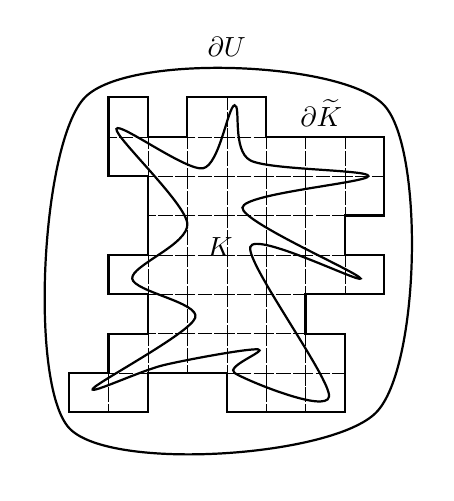
\begin{tikzpicture}
            \foreach \x in {0,...,7}
            \foreach \y in {0,...,7} {
                \ifnum\x=0
                \ifnum\y=1\else
                \ifnum\y=2\else
                \ifnum\y=3\else
                \ifnum\y=4\else
                \ifnum\y=5\else
                \ifnum\y=6\else
                \ifnum\y=7\else\draw[ultra thin, dashed] (0.5*\x,0.5*\y) rectangle ++(0.5,0.5);
                \fi\fi\fi\fi\fi\fi\fi \else
                \ifnum\x=1
                \ifnum\y=2\else
                \ifnum\y=4\else
                \ifnum\y=5\else\draw[ultra thin, dashed] (0.5*\x,0.5*\y) rectangle ++(0.5,0.5);
                \fi\fi\fi \else
                \ifnum\x=2
                \ifnum\y=0\else
                \ifnum\y=7\else\draw[ultra thin, dashed] (0.5*\x,0.5*\y) rectangle ++(0.5,0.5);
                \fi\fi \else
                \ifnum\x=3
                \ifnum\y=0\else\draw[ultra thin, dashed] (0.5*\x,0.5*\y) rectangle ++(0.5,0.5);
                \fi\else
                \ifnum\x=5
                \ifnum\y=7\else\draw[ultra thin, dashed] (0.5*\x,0.5*\y) rectangle ++(0.5,0.5);
                \fi\else
                \ifnum\x=6
                \ifnum\y=2\else
                \ifnum\y=7\else\draw[ultra thin, dashed] (0.5*\x,0.5*\y) rectangle ++(0.5,0.5);
                \fi\fi\else
                \ifnum\x=7
                \ifnum\y=0\else
                \ifnum\y=1\else
                \ifnum\y=2\else
                \ifnum\y=4\else
                \ifnum\y=7\else\draw[ultra thin, dashed] (0.5*\x,0.5*\y) rectangle ++(0.5,0.5);
                \fi\fi\fi\fi\fi\else
                \draw[ultra thin, dashed] (0.5*\x,0.5*\y) rectangle ++(0.5,0.5);
                \fi\fi\fi\fi\fi\fi\fi
            }
            \draw[thick] (0,0) -- (0,0.5) -- (0.5,0.5) -- (0.5,1) -- (1,1) -- (1,1.5) -- (0.5,1.5) -- (0.5,2) -- (1,2) -- (1,3) -- (0.5,3) -- (0.5,4) -- (1,4) -- (1,3.5) -- (1.5,3.5) -- (1.5,4) -- (2.5,4) -- (2.5,3.5) -- (4,3.5)-- (4,2.5) -- (3.5,2.5) -- (3.5,2) -- (4,2) -- (4,1.5) -- (3,1.5) -- (3,1) -- (3.5,1) -- (3.5,0) -- (2,0) -- (2,0.5) -- (1,0.5) -- (1,0) -- cycle;
            \draw[thick] plot[smooth cycle] coordinates {
                (3.8,3) (2.2,2.6) (3.7,1.7) (2.3,2.1) (3.3,0.2) (2.1,0.5) (2.4,0.8) (1.2,0.6) (0.3,0.3) (1.6,1.2) (0.8,1.7) (1.5,2.4) (0.6,3.6) (1.7,3.1) (2.1,3.9) (2.3,3.2)
            };
            \draw[thick] plot[smooth cycle] coordinates {
                (0,-0.2) (0.2,4) (4,3.9) (3.9,0)
            };
            \node[anchor=east] at (2.2,2.1) {\(K\)};
            \node[anchor=north] at (3.2,4.1) {\(\partial\widetilde{K}\)};
            \node[anchor=south] at (2,4.4) {\(\partial U\)};
        \end{tikzpicture}
        \caption{The elements of \(\mathcal{G}\), relative to \(K\) and its neighborhood, \(U\).}\label{fig:rungesimplepolesandremovablesingularityatinfinity_grid}
    \end{figure}Choose \(m\in\mathbb{N}\) to satisfy \(2^{1-m}<\sigma\) and consider the grid generated by compact squares in the form of \[\cbraces{x+\ii y}{\frac{j}{2^m}\leq x\leq\frac{j+1}{2^m},\frac{k}{2^m}\leq y\leq \frac{k+1}{2^m}}\] (where \(j\) and \(k\) are integers) and let \(\mathcal{G}\) be the collection of all such squares in this grid that intersect \(K\), and it follows that \(\widetilde{K}=\bigcup_{Q\in\mathcal{G}} Q\subset U\) (refer to \cref{fig:rungesimplepolesandremovablesingularityatinfinity_grid}).

    As a consequence of Cauchy--Goursat (\cref{thm:cauchygoursatformula}), we have
    \begin{equation}
        \frac{1}{2\piup\ii}\oint_{\partial \widetilde{K}}\frac{f(\zeta)\ddzeta}{\zeta-z}=f(z)\label{eq:rungesimplepolesandremovablesingularityatinfinity_cauchygoursat}
    \end{equation} in the case that \(z\in \widetilde{K}\). The boundary \(\partial \widetilde{K}\) may be written as the union of \(n\) lines parameterized by \(0\leq t\leq 1\); more concretely, we have \(\partial \widetilde{K}=\bigcup_{j\in\mathbb{N}_{\leq n}} \gamma_j([0,1])\). Hence we have in equivalent formulation, \[f(z)=\frac{1}{2\piup\ii}\sum_{j=1}^n\int_{\gamma_j([0,1])}\frac{f(\zeta)}{\zeta-z}\ddzeta=\frac{1}{2\piup\ii}\sum_{j=1}^n\int_0^1\frac{f\qty(\gamma_j(t))\gamma'_j(t)}{\gamma_j(t)-z}\ddt.\]
    The distance between \(K\) and \(\partial\widetilde{K}\) is strictly positive. Suppose instead that the distance were zero. Then some point of \(K\) would lie on the boundary of a square \(Q\in\mathcal{G}\) that intersects \(\partial\widetilde{K}\). If this point lies on an edge of \(Q\) (but not at a vertex), then the square adjacent along that edge must also intersect \(K\), and hence belong to \(\mathcal{G}\), contradicting the assumption that the point lies on \(\partial\widetilde{K}\). If the point lies at a vertex of \(Q\), then all three adjacent squares also intersect \(K\), so they too belong to \(\mathcal{G}\), leading to the same contradiction. Thus, the distance must be positive.

    Hence, each integrand as defined in \cref{eq:rungesimplepolesandremovablesingularityatinfinity_cauchygoursat} is jointly continuous for \(t\in[0,1]\) and \(z\in K\). By compactness of the product, it is in fact uniformly continuous by Heine--Cantor (\cref{thm:heinecantor}).

    Hence, \(\forall\varepsilon>0\), \(\exists\delta>0\) such that \(\forall z\in K\), \(\forall 1\leq j\leq n\) (uniform in \(j\) as we can take the minimum of each \(\delta_j\)), and \(\forall t_1,t_2\in [0,1]\) satisfying \(\abs{t_1-t_2}<\delta\), \[\abs{\frac{f\qty(\gamma_j\qty(t_1))\gamma'_j\qty(t_1)}{\gamma_j\qty(t_1)-z}-\frac{f\qty(\gamma_j\qty(t_2))\gamma'_j\qty(t_2)}{\gamma_j\qty(t_2)-z}}<\frac{\varepsilon}{n}.\]
    Partition \([0,1]\) by \(0=t_0<t_1<\cdots<t_m=1\) such that \(\forall 0\leq k<m\), \(\Delta t_k=t_{k+1}-t_k<\delta\). It follows that
    \begin{multline*}
        \abs{f(z)-\frac{1}{2\piup\ii}\sum_{j=1}^n \sum_{k=0}^{m-1}\frac{f\qty(\gamma_j\qty(t_k))\gamma'_j\qty(t_k)}{\gamma_j\qty(t_k)-z}\Delta t_k}\\
        =\frac{1}{2\piup}\abs{\sum_{j=1}^n\sum_{k=0}^{m-1}\int_{t_k}^{t_{k+1}}\qty[\frac{f\qty(\gamma_j\qty(t))\gamma'_j\qty(t)}{\gamma_j\qty(t)-z}-\frac{f\qty(\gamma_j\qty(t_k))\gamma'_j\qty(t_k)}{\gamma_j\qty(t_k)-z}]\ddt}\\
        \leq\frac{1}{2\piup}\sum_{j=1}^n\sum_{k=0}^{m-1}\int_{t_k}^{t_{k+1}}\abs{\frac{f\qty(\gamma_j\qty(t))\gamma'_j\qty(t)}{\gamma_j\qty(t)-z}-\frac{f\qty(\gamma_j\qty(t_k))\gamma'_j\qty(t_k)}{\gamma_j\qty(t_k)-z}}\ddt\\
        \leq \frac{\varepsilon}{2n\piup}\sum_{j=1}^n\sum_{k=0}^{m-1}\Delta t_k=\frac{\varepsilon}{2\piup}<\varepsilon
    \end{multline*} uniformly in \(z\in K\). The summation \[\psi(z)=\frac{1}{2\piup\ii}\sum_{j=1}^n \sum_{k=0}^{m-1}\frac{f\qty(\gamma_j\qty(t_k))\gamma'_j\qty(t_k)}{\gamma_j\qty(t_k)-z}\Delta t_k\] defines a rational function with simple poles at each \(\gamma_j\qty(t_k)\in\partial\widetilde{K}\), which is disjoint from \(K\).
\end{proof}
In its full generality, we will now apply a technique to \textit{push} a pole to a prescribed point, while ensuring that the resulting function remains uniformly approximated outside of a given connected compact set that contains both the original and target pole locations.
\begin{lemma}[Pole-Pushing Lemma]\label{lem:simplepolepushing}
    Let \(\alpha,\beta\in\mathbb{C}\) and let \(f(z)\) be a rational function with a single singularity, a pole at \(z=\alpha\), whose Laurent expansion consists solely of its principal part. Then \(\forall r>\abs{\alpha-\beta}\), \(\forall\varepsilon>0\), there exists a rational function \(\psi(z)\) whose only singularity is a pole at \(z=\beta\) such that \[\sup_{z\in\extcomplex\setminus D(\beta,r)}\abs{f(z)-\psi(z)}<\varepsilon.\]
\end{lemma}
\begin{proof}
    By assumption, \(f\) can be expressed as a polynomial of
    \begin{align*}
        (z-\alpha)^{-1}&=(z-\beta)^{-1}\frac{1}{\qty(z-\alpha)\qty(z-\beta)^{-1}}=\qty(z-\beta)^{-1}\frac{1}{1-\qty(\alpha-\beta)(z-\beta)^{-1}}\\
        &=\qty(z-\beta)^{-1}\sum_{k=0}^\infty\qty(\frac{\alpha-\beta}{z-\beta})^k.
    \end{align*}
    This series locally uniformly converges on \[\cbraces{z\in\extcomplex}{\abs{\alpha-\beta}\abs{z-\beta}^{-1}<1}=\extcomplex\setminus\overline{D\qty(\beta,\abs{\alpha-\beta})}\] and uniformly converges on \(\extcomplex\setminus D(\beta,r)\).
    Hence, for \(m\in\mathbb{N}\), we have \[f(z)=\sum_{j=1}^{m}a_{-j}\qty[\qty(z-\beta)^{-1}\sum_{k=0}^\infty\qty(\frac{\alpha-\beta}{z-\beta})^k]^j.\]
    For fixed \(j\) (where \(a_{-j}\neq 0\)), we aim to prove the existence of an \(N\in\mathbb{N}\) such that \(\forall n>N\), we have at least
    \begin{equation}
        \abs{\qty[(z-\beta)^{-1}\sum_{k=0}^\infty\qty(\frac{\alpha-\beta}{z-\beta})^k]^j-\qty[(z-\beta)^{-1}\sum_{k=0}^n\qty(\frac{\alpha-\beta}{z-\beta})^k]^j}<\frac{\varepsilon}{m\abs{a_{-j}}},\label{eq:simplepolepushing_uniformboundassumption}
    \end{equation} where \(z\in\extcomplex\setminus D(\beta,r)\). Since \(\abs{\frac{1}{z-\beta}}<\frac{1}{r}\), we can restrict \cref{eq:simplepolepushing_uniformboundassumption} further with \[\abs{\qty[\sum_{k=0}^\infty\qty(\frac{\alpha-\beta}{z-\beta})^k]^j-\qty[\sum_{k=0}^n\qty(\frac{\alpha-\beta}{z-\beta})^k]^j}<\frac{r^j\varepsilon}{m\abs{a_{-j}}}.\]
    Additionally, the difference on the left-hand side is also equal to
    \begin{equation}
        \abs{\qty(\sum_{k=n+1}^\infty\qty(\frac{\alpha-\beta}{z-\beta})^k)\qty(\sum_{l=0}^{j-1}\qty[\sum_{k=0}^n\qty(\frac{\alpha-\beta}{z-\beta})^k]^l\qty[\sum_{k=0}^\infty\qty(\frac{\alpha-\beta}{z-\beta})^k]^{j-l-1})}.\label{eq:simplepolepushing_uniformboundassumption2}
    \end{equation} For any \(n\in\mathbb{N}\), we have \[\abs{\sum_{k=0}^n\qty(\frac{\alpha-\beta}{z-\beta})^k}\leq\sum_{k=0}^n\abs{\frac{\alpha-\beta}{z-\beta}}^k\leq\sum_{k=0}^\infty\abs{\frac{\alpha-\beta}{r}}^k\leq\frac{1}{1-\abs{\frac{\alpha-\beta}{r}}}.\] Since the dominating sequence of partial sums are monotonically increasing, it follows that the sequence of partial sums is uniformly bounded by \[M=\frac{r}{r-\abs{\alpha-\beta}}\] on \(\extcomplex\setminus D(\beta,r)\). Thus, \cref{eq:simplepolepushing_uniformboundassumption2} is bounded by \(M^{j-1}j\abs{\sum_{k=n+1}^\infty\qty(\frac{\alpha-\beta}{z-\beta})^k}\), and we apply further restriction by setting this to be bounded by \(\frac{r^j\varepsilon}{m\abs{a_{-j}}}\).
    By uniform convergence, for any \(\varepsilon>0\), \(\exists N_j\in\mathbb{N}\) such that \(\forall n>N_j\), \[\abs{\sum_{k=n+1}^\infty\qty(\frac{\alpha-\beta}{z-\beta})^k}<\frac{r^j\varepsilon}{M^{j-1}jm\abs{a_{-j}}}.\] For \(n>N_j\), \cref{eq:simplepolepushing_uniformboundassumption} is satisfied, and \(\forall n>\max_{\substack{j=1\\a_{-j}\neq 0}}^m\qty(N_j)\), \(z\in\extcomplex\setminus D(\beta,r)\), we have
    \begin{align*}
        \abs{f(z)-\sum_{j=1}^ma_{-j}\qty[\frac{1}{z-\beta}\sum_{k=0}^n\qty(\frac{\alpha-\beta}{z-\beta})^k]^j}&\leq\sum_{\substack{j=1\\a_{-j}\neq 0}}^m\abs{a_{-j}}\abs{\qty[\sum_{k=0}^\infty\qty(\frac{\alpha-\beta}{z-\beta})^k]^j-\qty[\sum_{k=0}^n\qty(\frac{\alpha-\beta}{z-\beta})^k]^j}\\
        &\leq\sum_{\substack{j=1\\a_{-j}\neq 0}}^m\abs{a_{-j}}\frac{\varepsilon}{m\abs{a_{-j}}}\leq\varepsilon,
    \end{align*}
    which completes the proof as \[\psi(z)=\sum_{j=1}^ma_{-j}\qty[(z-\beta)^{-1}\sum_{k=0}^n\qty(\frac{\alpha-\beta}{z-\beta})^k]^j\] is rational with a pole at \(z=\beta\).
\end{proof}
\begin{lemma}[Generalized Pole-Pushing Lemma]\label{lem:generalpolepushing}
    Let \(K\subset\mathbb{C}\) be compact and choose \(a\in\mathbb{C}\setminus K\). Let \(U\) be the connected component of \(\extcomplex\setminus K\) containing \(a\). Then \(\forall\varepsilon>0\), \(\forall\xi\in U\), there exists a rational function \(\psi\) with a pole only at \(\xi\) such that \[\sup_{z\in K}\abs{\frac{1}{z-a}-\psi(z)}<\varepsilon.\]
\end{lemma}
\begin{proof}
    Define the set
    \[S=\cbraces{\xi\in U\setminus\qty{\infty}}{\forall\varepsilon>0,\exists\psi\text{ rational such that }
            \begin{aligned}
                &\psi(\mathbb{C}\setminus\qty{\xi})\subseteq\mathbb{C},\psi(\xi)=\infty,\\
                &\sup_{z\in K}\abs{\frac{1}{z-a}-\psi(z)}<\varepsilon
    \end{aligned}}.\]
    Since \(a\in U\) satisfies the condition with \(\psi(z)=\frac{1}{z-a}\), it follows that \(a\in S\), ensuring that \(S\) is nonempty.

    Consider \(\xi\in S\), where \(\xi\) lies in the complement of \(K\). The distance from \(\xi\) to \(K\), denoted \(\mathrm{dist}(\xi,K)\), is positive, and the open disk \(D(\xi,\mathrm{dist}(\xi,K))\) is disjoint from \(K\). Let \(\xi'\) be an arbitrary point in this disk. By the definition of \(S\), for every \(\varepsilon>0\), there exists a rational function \(\psi\) with a pole only at \(\xi\) such that
    \[\sup_{z\in K}\abs{\frac{1}{z-a}-\psi(z)}<\frac{\varepsilon}{2}.\]
    By \cref{lem:simplepolepushing}, there exists a rational function \(\phi\) with a pole only at \(\xi'\) such that
    \[\sup_{z\in\extcomplex\setminus D(\xi,\mathrm{dist}(\xi,K))}\abs{\phi(z)-\psi(z)}<\frac{\varepsilon}{2},\]
    which implies
    \[\sup_{z\in K}\abs{\phi(z)-\psi(z)}<\frac{\varepsilon}{2}.\]
    Thus,
    \[\sup_{z\in K}\abs{\frac{1}{z-a}-\phi(z)}\leq\sup_{z\in K}\abs{\frac{1}{z-a}-\psi(z)}+\sup_{z\in K}\abs{\psi(z)-\phi(z)}<\varepsilon,\]
    and by definition, \(\xi'\in S\Rightarrow D\qty(\xi,\mathrm{dist}\qty(\xi,K))\subseteq S\). Hence, \(S\) is relatively open in \(U\setminus\qty{\infty}\).

    Now, consider \(\xi\in U\setminus \qty(S\cup\qty{\infty})\). Suppose there exists \(\xi'\in D(\xi,\mathrm{dist}(\xi,K))\cap S\). By repeated application of the preceding argument, this would imply \(\xi\in S\), contradicting the assumption that \(\xi\in U\setminus \qty(S\cup\qty{\infty})\). Therefore, no such \(\xi'\) exists, and \(S\) is relatively closed in \(U\setminus\qty{\infty}\).

    Since \(U\setminus\qty{\infty}\) is connected and \(S\) is both relatively open and closed in \(U\setminus\qty{\infty}\), it follows from \cref{thm:connectedtopologicalspaceclopensets} that \(S=U\setminus\qty{\infty}\), completing the proof under the assumption that \(\infty\notin U\).

    Now suppose \(\infty\in U\). In essence, we pole push to a point outside a disk on which we can make approximations by Taylor polynomials. Let \(R>0\) satisfy \(K\subset D(0,R)\) and let \(b\in U\setminus\qty(\qty{\infty}\cup \overline{D(0,R)})\) be an arbitrary point. By \cref{lem:simplepolepushing}, there exists some rational function \(\widetilde{\psi}(z)\) with a pole at \(b\) such that \[\sup_{z\in K}\abs{\widetilde{\psi}(z)-\frac{1}{z-a}}<\frac\varepsilon2.\]
    Since \(\widetilde{\psi}\) is holomorphic on some neighborhood of \(\overline{D(0,R)}\), we have \[\widetilde{\psi}(z)=\sum_{k=0}^\infty a_k z^k\qq{on}\overline{D(0,R)}\] and it uniformly converges on \(\overline{D(0,R)}\). Hence, \(\exists N\in\mathbb{N}\) such that \[\sup_{z\in\overline{D(0,R)}}\abs{\widetilde{\psi}(z)-\sum_{k=0}^N a_k z^k}<\frac{\varepsilon}{2}.\]
    Since polynomials have poles at \(\infty\), we have \[\sup_{z\in\overline{D(0,R)}}\abs{\frac{1}{z-a}-\sum_{k=0}^N a_k z^K}\leq\sup_{z\in\overline{D(0,R)}}\abs{\frac{1}{z-a}-\widetilde{\psi}(z)}+\sup_{z\in\overline{D(0,R)}}\abs{\widetilde{\psi}(z)-\sum_{k=0}^N a_kz^k}<\varepsilon.\qedhere\]
\end{proof}
\begin{theorem}[Runge]\label{thm:runge}
    Let \(K\subset\mathbb{C}\) be compact and suppose \(f\) is holomorphic on a neighborhood of \(K\). Let \(E\) be a subset of \(\extcomplex\setminus K\) containing one point from each of its connected components. Then \(\forall\varepsilon>0\), there is a rational function \(\psi\) whose poles lie in \(E\) such that \[\sup_{z\in K}\abs{f(z)-\psi(z)}<\varepsilon.\]
\end{theorem}
\begin{proof}
    By \cref{prop:rungesimplepolesandremovablesingularityatinfinity}, there is a rational function \(\phi\) with simple poles in \(\mathbb{C}\setminus K\) satisfying \(\phi(\infty)=0\) such that
    \begin{equation}
        \sup_{z\in K}\abs{f(z)-\phi(z)}<\frac\varepsilon2.\label{eq:runge_intermediate1}
    \end{equation}
    Let the poles of \(\phi\) be \(\qty{\beta_k}_{k\in\mathbb{N}_{\leq n}}\subset\mathbb{C}\setminus K\), and as a consequence, we have \(\phi(z)=\sum_{k=1}^n\frac{a_k}{z-\beta_k}+\varphi(z)\) where \(\varphi(z)\) is entire. Since \(\phi(\infty)=0\), we have \(\varphi\equiv 0\) by Liouville's Theorem (\cref{thm:liouville}). By \cref{lem:generalpolepushing}, there exist rational functions \(\qty{\psi_k}_{k\in\mathbb{N}_{\leq n}}\) whose only poles lie in \(E\) such that \(\forall k\), \[\sup_{z\in K}\abs{\frac{1}{z-\beta_k}-\psi_k(z)}<\frac{\varepsilon}{2n\abs{a_k}}\] and it follows that \[\sup_{z\in K}\abs{\phi(z)-\sum_{k=1}^n a_k\psi_k(z)}\leq\sup_{z\in K}\sum_{k=1}^n\abs{\frac{a_k}{z-\beta_k}-a_k\psi_k(z)}<\frac\varepsilon2.\]
    Let \(\psi(z)=\sum_{k=1}^na_k\psi_k(z)\). From \cref{eq:runge_intermediate1}, we have \[\sup_{z\in K}\abs{f(z)-\psi(z)}\leq\sup_{z\in K}\abs{f(z)-\phi(z)}+\sup_{z\in K}\abs{\phi(z)-\psi(z)}<\varepsilon.\qedhere\]
\end{proof}
\subsection{Mergelyan's Theorem}
Although many mathematicians have since tried after the efforts of Weierstrass and Runge to approximation continuous functions holomorphic on the interior restriction, it was only 67 years later when Armenian mathematician provided the first widely accepted proof. The proof of Runge's Theorem (specifically in \cref{prop:rungesimplepolesandremovablesingularityatinfinity}) relied heavily on the assumption of holomorphy on a neighborhood, a rational function was created by placing poles in prescribed points of a contour that lay outside of \(K\) but within its domain of holomorphy. Obviously, these assumptions are null under the context of this new formulation.

The proof proposed by Mergelyan is almost trivial when compared with the results of many other mathematicians at the time. It even uses the concepts previously proposed by Runge. This begs the question: why was there such a prolonged time gap between the two similar formulations? Many mathematicians felt that the conclusion was too ethereal; during this elapsed time period there were many efforts of mathematicians that resulted in many technical partial results. Mergelyan's Theorem came as a surprise as it encapsulated many of those results with simplicity.

As we have previously seen, there is a prevalent notion in complex analysis that regards \(\infty\) intrinsically as essentially any other point of \(\extcomplex\). An appertaining question relates to the complex derivative at \(\infty\). Although \[f'(\infty)\overset{?}{=}\lim_{z\to\infty} f'(z)\] may seem to be a natural object to consider, it is quite impractical; there exist functions which decay quickly to 0, while \(f'(z)\) is unbounded as \(z\to\infty\) (take \(z\mapsto\frac{\sin\qty(z^2)}{\sqrt{z}}\) as an example). Even the assumption that \(\lim_{z\to\infty}f'(z)=0\) does not imply that \(f(z)\) has a removable singularity at \(\infty\) (consider \(z\mapsto\sqrt{z}\)).
\begin{definition}
    Let \(R>0\), \(f:\mathbb{C}\setminus\overline{D(0,R)}\to\mathbb{C}\) be holomorphic such that \(f\) has a removable singularity at \(\infty\). Then we define the derivatives of \(f\) at \(\infty\) to be \[f^{(n)}(\infty)=\eval{\dv[n]{z}f\qty(\frac1z)}_{z=0}.\]
    In the case that \(n=1\), we have \[f'(\infty)=-\lim_{z\to\infty}z^2 f'\qty(z).\]
\end{definition} This is precisely the first singular term of the Laurent expansion of \(f\) at \(\infty\).
\begin{remark}
    This definition may feel unsatisfactory, but the underlying logic here is similar to the method used to generalize residues to \(\infty\).
\end{remark}
If \(f\) is bijective and meromorphic on some neighborhood of a point \(a\in\mathbb{C}\) such that \(f(a)=\infty\), then we informally define the derivative at the pole \(a\) to be
\begin{equation}
    f'(a)=\frac{1}{\qty(f^{-1})'\qty(\infty)}=-\lim_{w\to\infty}\frac{1}{w^2\qty(f^{-1})'(w)}=-\lim_{w\to\infty}\frac{f'\qty(f^{-1}(w))}{w^2}.\label{eq:derivativeatpole1}
\end{equation}
Let \(z=f^{-1}(w)\). Then we have
\begin{equation}
    f'(a)=-\lim_{z\to a}\frac{f'(z)}{f(z)^2}=\eval{\dv{z}(\frac{1}{f(z)})}_{z=a}.\label{eq:derivativeatpole2}
\end{equation}
\begin{proposition}\label{prop:complementbiholomorphismquarterestimate}
    For any connected compact set \(K\subset\mathbb{C}\) containing at least two distinct points such that \(\extcomplex\setminus K\) is connected, let \(\phi\) be an arbitrary biholomorphism mapping \(\extcomplex\setminus K\) to \(\mathbb{D}\) such that \(\phi(\infty)=\lim_{z\to\infty}\phi(z)=0\). It follows that \[\abs{\phi'(\infty)}\geq\frac14\diam(K),\] where \(\diam(K)=\sup_{z,\zeta\in K}\abs{\zeta-z}\).
\end{proposition}
\begin{proof}
    Denote the derivative of \(\phi\) at the infinity to be \(\alpha\). By \cref{eq:derivativeatpole1}, we have \[\qty(\phi^{-1})'(0)=\frac{1}{\phi'(\infty)}=\frac1\alpha=-\lim_{z\to 0}\frac{\qty(\phi^{-1})'(z)}{\phi^{-1}(z)^2}\Longleftrightarrow-\lim_{z\to0}\frac{\phi^{-1}(z)^2}{\alpha\qty(\phi^{-1})'(z)}=1.\]
    Fix \(\tau\in K\) and let \(\psi(z)=\frac{\alpha}{\phi^{-1}(z)-\tau}\), univalent on \(\mathbb{D}\). By direct calculation, we have \(\psi(0)=0\). Additionally,
    \begin{align*}
        \psi'(0)=-\lim_{z\to 0}\frac{\alpha\qty(\phi^{-1})'(z)}{\qty(\phi^{-1}(z)-\tau)^2}=\lim_{z\to 0}\frac{\alpha\qty(\phi^{-1})'(z)}{\qty(\phi^{-1}(z)-\tau)^2}\cdot\frac{\phi^{-1}(z)^2}{\alpha\qty(\phi^{-1})'(z)}=1.
    \end{align*}
    By the Koebe Quarter Theorem (\cref{thm:koebequarter}), whose proof is independent of results of this section, in accordance, \(D\qty(0,\frac14)\subseteq\psi(\mathbb{D})\). Let \(\mu\in K\setminus\qty{\tau}\). Obviously, \(\mu\notin\phi^{-1}(\mathbb{D})=\extcomplex\setminus K\).

    Let \(z\mapsto\frac{\alpha}{z-\tau}\) be injective on \(\extcomplex\). For the sake of contradiction, assume that \(\qty(z\mapsto\frac{\alpha}{z-\tau})(\mu)\in\psi(\mathbb{D})\). Then \(\exists\zeta\in\phi^{-1}(\mathbb{D})\) such that \(\frac{\alpha}{\zeta-\tau}=\frac{\alpha}{\mu-\tau}\). By injectivity, \(\zeta=\mu\), which contradicts \(\mu\in K\), and accordingly, \(\frac{\alpha}{\mu-\tau}\notin\psi(\mathbb{D})\supseteq D\qty(0,\frac14)\).

    Hence, \[\abs{\frac{\alpha}{\mu-\tau}}\geq\frac14\Longleftrightarrow\abs{\alpha}\geq\frac{\abs{\mu-\tau}}{4}.\] By taking the supremum for \(\mu,\tau\in K\), the proof is complete.
\end{proof}
\begin{remark}
    Such a biholomorphism will always exist; for arbitrary \(\zeta\in K\), the map \(z\mapsto\frac{1}{z-\zeta}\) maps \(\extcomplex\setminus K\) to a simply connected, proper subset of \(\mathbb{C}\), which is biholomorphic to \(\mathbb{D}\) by the Riemann Mapping Theorem (\cref{thm:riemannmapping}).
\end{remark}
\begin{proposition}\label{prop:complementbiholomorphism584r4767r2estimates}
    Let \(a\in\mathbb{C}\), \(r>0\), and suppose \(K\subseteq D(a,r)\) is compact such that \(\extcomplex\setminus K\) is connected and \(\diam(K)\geq\frac r2\). Then there is a family of holomorphic functions \(\mathcal{F}=\qty{f_\zeta}_{\zeta\in D(a,r)}\), where \(\forall\zeta\in D(a,r)\), \[f_\zeta:\extcomplex\setminus K\to\mathbb{C},\] and
    \begin{enumerate}
        \item \(\abs{f_\zeta(z)}<\frac{584}{r}\) for any \(z\in\extcomplex\setminus K\).\label{itm:complementbiholomorphismquarterestimate_absolute584}
        \item \(\abs{f_\zeta(z)-\frac{1}{z-\zeta}}<\frac{4676r^2}{\abs{\zeta-z}^3}\) for any \(z\in\extcomplex\setminus\qty(K\cup\qty{\zeta})\).\label{itm:complementbiholomorphismquarterestimate_absolutedifference4676}
        \item The function \(f(\zeta,z)\equiv f_\zeta(z)\) is jointly continuous in \(\zeta\) and \(z\).
    \end{enumerate}
\end{proposition}
\begin{proof}
    For brevity, assume \(a=0\).

    Let \(\widetilde{\varphi}\) be a conformal mapping from \(\extcomplex\setminus K\) to \(\mathbb{D}\), such that \(\widetilde{\varphi}(\infty)=0\) and \(\alpha=\widetilde{\varphi}'(\infty)\in\mathbb{R}_{>0}\). Let \(\varphi(z)=\frac{1}{\alpha}\widetilde{\varphi}(z)\). It follows that \(\varphi'(\infty)=1\), \(\varphi(\infty)=0\). By \cref{prop:complementbiholomorphismquarterestimate}, \[\abs{\alpha}\geq\frac{1}{4}\diam(K)\Longleftrightarrow\abs{\varphi(z)}\leq\frac{4\abs{\widetilde{\varphi}(z)}}{\diam(K)}.\] Consequently, we have the crucial estimate of \(\varphi\qty(\extcomplex\setminus K)\subseteq D\qty(0,\frac{4}{\diam(K)})\subseteq D\qty(0,\frac{8}{r})\). For fixed \(\zeta\in D(0,r)\), define \[f_\zeta(z)=\varphi(z)+(\zeta-\beta)\varphi^2(z),\qquad z\in\extcomplex\setminus K\] where \(\beta=\frac{\varphi''(\infty)}{2}\). Cauchy's Estimate (\cref{thm:cauchysestimate}) on \(\qty(z\mapsto\frac{1}{z})\qty(\extcomplex\setminus D(0,r))=D\qty(0,\frac{1}{r})\) gives: \[\abs{\beta}=\frac{1}{2}\abs{\eval{\dv[2]{z}(\varphi\qty(\frac{1}{z}))}_{z=0}}\leq\frac{\sup_{D\qty(0,\frac1r)}\abs{\varphi\qty(\frac{1}{z})}}{\operatorname{dist}\qty(0,\partial D\qty(0,\frac{1}{r}))^2}=8r.\]
    Hence, \[\abs{f_\zeta(z)}\leq \abs{\varphi(z)}+\abs{\zeta-\beta}\abs{\varphi^2(z)}\leq\abs{\varphi(z)}+\abs{\zeta-\beta}\abs{\varphi^2(z)}\leq\frac{8}{r}+9r\frac{64}{r^2}=\frac{584}{r}.\] This is~\ref{itm:complementbiholomorphismquarterestimate_absolute584}. Suppose that \(\abs{z-\zeta}>2r\). It follows from \(\abs{\zeta}<r\) that \(\abs{z}>r\) (from the reverse triangle inequality) and hence disjoint from \(K\) and \(\zeta\). On this infinite annulus, we have the Laurent expansion (from \cref{thm:laurentexpansionofholomorphicfunction}) that \[\varphi(z)=\sum_{k=1}^\infty\frac{\mu_k}{\qty(z-\zeta)^k}=\frac{1}{z-\zeta}+\frac{\mu}{(z-\zeta)^2}+\order{\frac1{\qty(z-\zeta)^3}}\] where \(\mu_1=1\) because \(\varphi\sim\frac{1}{z}\) as \(z\to\infty\). Since \(\abs{z}>r\), we have the global Laurent expansion \[\varphi(z)=\frac1z+\frac\beta{z^2}+\order{\frac1{z^3}}.\]
    Hence,
    \begin{align*}
        \frac1{z-\zeta}+\frac\mu{\qty(z-\zeta)^2}&=\frac1z+\frac\beta{z^2}+\order{\frac1{z^3}}\\
        z+\zeta+\mu&=z+\frac{\zeta^2}z+\beta+\frac{\beta\zeta^2}{z^2}-\frac{2\beta\zeta}{z}+\order{\frac1z}=z+\beta+\order{\frac1z}\\
        \mu&=\beta-\zeta
    \end{align*} by letting \(z\to\infty\). Since \[\varphi^2(z)=\qty(\frac{1}{z-\zeta}+\order{\frac1{\qty(z-\zeta)^2}})^2=\frac{1}{\qty(z-\zeta)^2}+\order{\frac{1}{\qty(z-\zeta)^3}},\] from the definition of \(f_\zeta\), we have
    \begin{align*}
        f_\zeta(z)-\frac{1}{z-\zeta}=\varphi-\mu\varphi^2-\frac{1}{z-\zeta}&=\frac{\mu}{\qty(z-\zeta)^2}+\order{\frac1{(z-\zeta)^3}}-\frac{\mu}{\qty(z-\zeta)^2}-\order{\frac{\mu}{\qty(z-\zeta)^3}}\\
        &=\order{\frac1{\qty(z-\zeta)^3}}.
    \end{align*}
    Hence, there exists some \(M>0\) such that \[\abs{f_\zeta(z)-\frac{1}{z-\zeta}}<\frac{M}{\abs{z-\zeta}^3}\Longleftrightarrow\abs{f_\zeta(z)-\frac{1}{z-\zeta}}\abs{z-\zeta}^3<M\] for all \(z\) satisfying \(\abs{z-\zeta}>2r\). By \cref{thm:riemannremovablesingularities}, \(\qty(f_\zeta(z)-\frac{1}{z-\zeta})\qty(z-\zeta)^3\) has a removable singularity at \(\infty\). On the other hand, for \(\abs{z-\zeta}\leq 2r\) such that \(z\in\extcomplex\setminus\qty(K\cup\qty{\zeta})\), we have \[\abs{f_\zeta(z)-\frac{1}{z-\zeta}}\abs{z-\zeta}^3\leq\abs{f_\zeta(z)}\abs{z-\zeta}^3+\abs{z-\zeta}^2\leq\frac{584}{r}(2r)^3+(2r)^2=4676r^2\] from \ref{itm:complementbiholomorphismquarterestimate_absolute584}. The Maximum Modulus Principle (\cref{thm:maximummodulus}) implies that \[\sup_{\abs{z-\zeta}>2r}\abs{f_\zeta(z)-\frac{1}{z-\zeta}}\abs{z-\zeta}^3\leq\sup_{\abs{z-\zeta}=2r}\abs{f_\zeta(z)-\frac{1}{z-\zeta}}\abs{z-\zeta}^3\leq 4676r^2\] and thus \ref{itm:complementbiholomorphismquarterestimate_absolutedifference4676} follows. The joint continuity of \(f_\zeta\) is immediate from the definition.

    Lastly, if \(a\neq 0\), we may define \(f_\zeta(z)=\widetilde{f}_{\zeta-a}(z-a)\) where \(\qty{\widetilde{f}_{\zeta-a}}\) is the family constructed above for the set \(\cbraces{z-a}{z\in K}\subset D(0,r)\).
\end{proof}
\begin{proposition}\label{prop:diracdeltaapproximation}
    Suppose
    \begin{equation}
        \lambda(z)=
        \begin{cases}
            \qty(1-\abs{z}^2)^2&\qif*\abs{z}<1\\
            0&\qif*\abs{z}\ge1,
        \end{cases}\qquad\lambda_r(z)=\frac{3}{\piup r^2}\lambda\qty(\frac{z}{r})\quad\forall r>0\label{eq:diracdeltaapproximation_lambdadefinition}
    \end{equation}
    For fixed \(r\), the function \(\lambda_r\) satisfies:
    \begin{enumerate}
        \item \(\int_{\mathbb{C}}\lambda_r(\zeta)\dd{\xi}\wedge\dd{\eta}=1\), where \(\zeta=\xi+\ii\eta\).\label{itm:diracdeltaapproximation_integralto1}
        \item \(\lambda_r\in C^1(\mathbb{C})\) and is compactly supported.\label{itm:diracdeltaapproximation_compactsupportcontinuousdifferentiability}
        \item \(\int_{\mathbb{C}}\pdv{\lambda_r}{\overline{\zeta}}\dd{\xi}\wedge\dd{\eta}=0\).\label{itm:diracdeltaapproximation_antiholomorphicderivativeintegral}
        \item \(\int_{\mathbb{C}}\abs{\pdv{\lambda_r}{\overline{\zeta}}}\dd{\xi}\wedge\dd{\eta}\leq\frac{2\piup}{r}\).\label{itm:diracdeltaapproximation_absoluteantiholomorphicderivativeintegral}
        \item \(\abs{\grad{\lambda_r(z)}}\leq\frac4{r^3}\) for all \(z\), where \(\grad=\qty(\pdv{}{x},\pdv{}{y})\) denotes the vector differential operator.\label{itm:diracdeltaapproximation_gradientstatement}
        \item\label{itm:diracdeltaapproximation_integralformula} For any \(z\in\mathbb{C}\) such that \(f\) is a holomorphic function on \(D(z,r)\), we have the integral formula
            \begin{equation}
                f(z)=\int_{D(0,r)}f(z-\zeta)\lambda_r(\zeta)\dd{\xi}\wedge\dd{\eta}.\label{eq:diracdeltaapproximation_integralformula}
            \end{equation}
    \end{enumerate}
\end{proposition}
\begin{proof}
    Let \(\zeta=\rho\ee^{\ii\theta}\). Then we have
    \begin{align*}
        \iint_{\mathbb{C}}\lambda_r(\zeta)\dd{\xi}\dd{\eta}&=\int_{0}^{2\piup}\int_0^r \lambda_r\qty(\rho\ee^{\ii\theta})\rho\dd{\rho}\dd{\theta}=\int_{0}^{2\piup}\int_0^r\frac{3\rho}{\piup r^2}\qty(1-\qty(\frac{\rho}{r})^2)^2\dd{\rho}\dd{\theta}\\
        &=\frac{6}{r^2}\int_0^r\qty(\rho+\frac{\rho^5}{r^4}-2\frac{\rho^3}{r^2})\dd{\rho}=\frac{6}{r^2}\qty(\frac{r^2}{2}+\frac{r^6}{6r^4}-\frac{r^4}{2r^2})=1,
    \end{align*}
    which confirms property~\ref{itm:diracdeltaapproximation_integralto1}. Let \(z\in\mathbb{C}\) be arbitrary. The integral in \cref{eq:diracdeltaapproximation_integralformula} is equal to
    \begin{align*}
        \iint_{D(0,R)}f(z-\zeta)\lambda_r(\zeta)\dd{\xi}\dd{\eta}&=\int_0^r\frac{3\rho}{\piup r^2}\qty(1-\qty(\frac{\rho}{r})^2)^2\int_0^{2\piup}f\qty(z-\rho\ee^{\ii\theta})\dd{\theta}\dd{\rho}\\
        &=2\piup f(z)\int_0^r\frac{3\rho}{\piup r^2}\qty(1-\qty(\frac{\rho}{r})^2)^2\dd{\rho}=f(z)
    \end{align*} by the mean-value property (\cref{lem:holomorphicmeanvalueproperty}), proving~\ref{itm:diracdeltaapproximation_integralformula}. For \(z\in\mathbb{D}\), we have \[\abs{\grad{\lambda(z)}}=
    2\qty(1-\abs{z}^2)\abs{\grad(\abs{z}^2)}=2\qty(1-\abs{z}^2)2\abs{z}\abs{\grad\sqrt{x^2+y^2}}=4\qty(1-\abs{z}^2)\abs{z}.\]
    Hence, \(\abs{\grad\lambda_r(z)}=\frac{3}{\piup r^2}\abs{\grad\qty[\lambda\qty(\frac{z}{r})]}=\frac{3}{\piup r^2}\abs{(\grad\lambda)\qty(\frac{z}{r})}\frac{1}{r}=\frac{12}{\piup r^3}\qty(1-\abs{z}^2)\abs{z}<\frac{4}{r^3}\), which confirms \ref{itm:diracdeltaapproximation_gradientstatement}.

    Since \(\abs{\pdv{\lambda_r}{\overline{\zeta}}}=\abs{\frac{1}{2}\qty(\pdv{\lambda_r}{\xi}+\ii\pdv{\lambda_r}{\eta})}=\frac{1}{2}\abs{\grad\lambda_r(\zeta)}<\frac{2}{r^3}\), we have \[\iint_{\mathbb{C}}\abs{\pdv{\lambda_r}{\overline{\zeta}}}\dd{\xi}\dd{\eta}=\iint_{D(0,r)}\abs{\pdv{\lambda_r}{\overline{\zeta}}}\dd{\xi}\dd{\eta}<\piup r^2\frac{2}{r^3}=\frac{2\piup}{r}\] since \(\supp\qty(\lambda_r)=\overline{D(0,r)}\) which verifies the inequality in property ~\ref{itm:diracdeltaapproximation_absoluteantiholomorphicderivativeintegral}.

    The property~\ref{itm:diracdeltaapproximation_antiholomorphicderivativeintegral} is also true since
    \begin{align*}
        \iint_{\mathbb{C}}\pdv{\lambda_r}{\overline{\zeta}}\dd{\xi}\dd{\eta}&=\frac{1}{2}\int_{-r}^r\int_{-r}^{r}\pdv{\lambda_r}{\xi}\dd{\xi}\dd{\eta}+\frac{\ii}{2}\int_{-r}^r\int_{-r}^{r}\pdv{\lambda_r}{\eta}\dd{\eta}\dd{\xi}\\
        &=\frac{1}{2}\int_{-r}^r\qty[\lambda_r\qty(r+\ii\eta)-\lambda\qty(-r+\ii\eta)]\dd{\eta}\\
        &\quad+\frac{\ii}{2}\int_{-r}^r\qty[\lambda_r(\xi+\ii r)-\lambda_r(\xi-\ii r)]\dd{\xi}=0.
    \end{align*}
    Trivially, \(\lambda_r\) is continuous on \(D\qty(0,r)\) and \(\mathbb{C}\setminus\overline{D(0,r)}\). Thus, we only need to prove the joint continuity of \(\lambda\) (the continuity of \(\lambda_r\) implies that of \(\lambda\)) on an open neighborhood of \(\partial D(0,r)\).

    Let \(\lambda(x,y)=\qty(1-x^2-y^2)^2\). By simple calculation, we have \[\pdv{\lambda}{x}=-4\qty(1-x^2-y^2)x,\qquad\pdv{\lambda}{y}=-4\qty(1-x^2-y^2)y.\] At \(x^2+y^2=1\), both partial derivatives vanish, and hence, they match the vanishing derivative on the complement of \(\supp(\lambda)\), completing the proof of property~\ref{itm:diracdeltaapproximation_compactsupportcontinuousdifferentiability}.
\end{proof}
\begin{theorem}[\textsc{Tietze--Urysohn--Brouwer}]\label{thm:tietzeextension}
    Let \(K\subset\mathbb{C}\) be compact and \(f:K\to\mathbb{R}\) be continuous. Then \(\exists g\in C^0(\mathbb{C})\) such that \(g\equiv f\) on \(K\).
\end{theorem}
\begin{proof}
    For any two disjoint closed \(A,B\subseteq\mathbb{C}\), consider the continuous separation function \[\eta_{A,B}(z)=\frac{\operatorname{dist}(z,A)-\operatorname{dist}(z,B)}{\operatorname{dist}(z,A)+\operatorname{dist}(z,B)}\] so that \(\eta_{A,B}(A)=\qty{-1}\) and \(\eta_{A,B}(B)=\qty{1}\).

    For simplicity, by the boundedness of \(f\), we may assume that \(f(K)=[-1,1]\) (by a scaling and shift). We now aim to construct a sequence \(\qty{g_n}_{n\in\mathbb{N}_{\geq 0}}\) inductively such that \[\abs{g_n}\leq\frac{2^n}{3^{n+1}}\text{ on }\mathbb{C},\quad\abs{f-\sum_{k=0}^n g_k}\leq\qty(\frac23)^{n+1}\text{ on }K\quad\forall n\in\mathbb{N}.\]
    In the case that \(n=0\), define the disjoint closed sets \[A_0=\cbraces{z\in K}{f(z)\leq-\frac13}\qand B_0=\cbraces{z\in K}{f(z)\geq\frac13}.\]
    Let \(g_0(z)=\frac13\eta_{A_0,B_0}(z)\). It is clear that \(\abs{g_0}\leq\frac13\) on \(\mathbb{C}\). If \(z\in A_0\), then \(-1\leq f(z)\leq-\frac13\), \(g_0(z)=-\frac13\), and hence \(\abs{f-g_0}\leq\frac23\). If \(z\in B_0\), then \(\frac13\leq f(z)\leq1\), \(g_0(z)=\frac13\), and thus \(\abs{f-g_0}\leq\frac23\). If \(z\notin A_0\cup B_0\), then \(-\frac13<f(z)<\frac13\) and \(\abs{f-g_0}\leq\abs{f}+\abs{g_0}<\frac13+\frac13=\frac23\). Hence \(\forall z\in K\), \[\abs{f(z)-g_0(z)}\leq\frac23.\]
    This proves the base case. For the inductive step, assume the claim holds for each \(g_0,g_1,\dots,g_{n-1}\). Define \[h_n(z)=f(z)-\sum_{k=0}^{n-1}g_k(z)\] for \(z\in K\). By the inductive hypothesis, we have \(\abs{h_n}\leq\qty(\frac23)^n\) on \(K\). Define the disjoint closed sets \[A_n=\cbraces{z\in K}{-\frac{2^n}{3^n}\leq h_n(z)\leq-\frac{2^n}{3^{n+1}}}\qand B_n=\cbraces{z\in K}{\frac{2^n}{3^n}\geq h_n(z)\geq\frac{2^n}{3^{n+1}}}.\]
    Let \(g_n(z)=\frac{2^n}{3^{n+1}}\eta_{A_n,B_n}(z)\), so that \(\abs{g_n}\leq\frac{2^n}{3^{n+1}}\) on \(\mathbb{C}\), and \[\abs{h_n(z)-g_n(z)}\leq\frac{2^{n+1}}{3^{n+1}}\] for all \(z\in K\) by the same argument as in the base case. Hence, \[\abs{f(z)-\sum_{k=0}^n g_k(z)}=\abs{h_n(z)-g_n(z)}\leq\qty(\frac23)^{n+1}\] for all \(z\in K\), completing the induction. Because \[\abs{g(z)}\leq \sum_{n=0}^\infty\abs{g_n(z)}\leq\frac13\sum_{n=0}^\infty\frac{2^n}{3^n}=1\qquad\forall z\in\mathbb{C},\] the Weierstrass \(M\)--Test (\cref{thm:weierstrassmtest}) implies that the series \(\sum_{n=0}^\infty g_n(z)\) converges uniformly on \(\mathbb{C}\) to \(g\). Since each \(g_n\) is continuous, \cref{thm:uniformlimit} gives the continuity of \(g\) on \(\mathbb{C}\). Finally, for any \(z\in K\), we have \[\abs{f(z)-g(z)}\leq\lim_{n\to\infty}\frac{2^{n+1}}{3^{n+1}}=0.\qedhere\]
\end{proof}
\begin{corollary}\label{cor:tietzeextensioncomplexcompactsupport}
    If \(K\subset\mathbb{C}\) is compact and \(f:K\to\mathbb{C}\) is continuous, then \(\exists g\in C^0(\mathbb{C})\) such that \(g\equiv f\) on \(K\) and has compact support.
\end{corollary}
\begin{proof}
    Let \(f=u+\ii v\) where \(u,v:K\to\mathbb{R}\) are continuous. By Tietze--Urysohn--Brouwer (\cref{thm:tietzeextension}), \(\exists \widetilde{u},\widetilde{v}\in C^0(\mathbb{C})\) such that \(\widetilde{u}\equiv u\) and \(\widetilde{v}\equiv v\) on \(K\). Let \(R>0\) be such that \(K\subset D(0,R)\), provided by compactness. Define the piecewise-linear function \[\psi(z)=
        \begin{cases}
            1&\qif*\abs{z}\leq R\\
            2-\frac{\abs{z}}{R}&\qif*R<\abs{z}<2R\\
            0&\qif*\abs{z}\geq 2R
    \end{cases}\] such that \(\psi\in C^0(\mathbb{C})\) and is compactly supported. Let \(g(z)=\qty(\widetilde{u}(z)+\ii\widetilde{v}(z))\psi(z)\), and the assertion follows.
\end{proof}
Let \(f\in C^0(K)\) be holomorphic on \(\interior{K}\). Then \(f\) has a continuous extension to all of \(\mathbb{C}\) by virtue of \cref{cor:tietzeextensioncomplexcompactsupport}. Define the \textscsl{modulus of continuity} of \(f\) to be the function \(\omega_f:\mathbb{R}_{\geq0}\to\mathbb{R}_{\geq0}\) with \[\omega_f(\delta)=\sup_{\substack{z,\zeta\in\mathbb{C}\\\abs{z-\zeta}\leq\delta}}\abs{f(z)-f(\zeta)}.\]
Because \(f\) has compact support, it must be uniformly continuous; hence we have \(\lim_{\delta\to0^+}\omega_f(\delta)=0\).

For \(r>0\), define
\begin{equation}
    \Phi(z)=\iint_\mathbb{C}\lambda_r(z-\zeta)f(\zeta)\dd{\xi}\dd{\eta}\qq{where}\zeta=\xi+\ii\eta,\label{eq:integralofcontinuousextensionofholomorphic}
\end{equation} where \(\lambda_r\) employs the same definition as in \cref{eq:diracdeltaapproximation_lambdadefinition}.
\begin{proposition}\label{prop:integralofcontinuousextensionofholomorphicproperties}
    The function \(\Phi\) as in \cref{eq:integralofcontinuousextensionofholomorphic} satisfies:
    \begin{enumerate}
        \item \(\Phi\in\mathbb{C}^1(\mathbb{C})\) and has compact support.\label{itm:integralofcontinuousextensionofholomorphicproperties_continuousdifferentiabilitycompactsupport}
        \item \(\Phi\equiv f\) on \(U=\cbraces{z\in K}{\operatorname{dist}\qty(z,\mathbb{C}\setminus K)>r}\).\label{itm:integralofcontinuousextensionofholomorphicproperties_equivalenceonU}
        \item \(\abs{f(z)-\Phi(z)}\leq\omega_f(r)\) for all \(z\in\mathbb{C}\).\label{itm:integralofcontinuousextensionofholomorphicproperties_differbymodulusofcontinuity}
        \item For all \(z\in\mathbb{C}\), \(\abs{\pdv{\Phi}{\overline{z}}(z)}\leq\frac{4\piup\omega(r)}{r}\).\label{itm:integralofcontinuousextensionofholomorphicproperties_antiholomorphicderivativebound}
        \item \(\Phi(z)=-\frac1\piup\iint_H\pdv{\Phi}{\overline{\zeta}}(\zeta)\frac{\dd{\xi}\dd{\eta}}{\zeta-z}\) for \(z\in\mathbb{C}\), where \(H=\supp(\Phi)\setminus U\).\label{itm:integralofcontinuousextensionofholomorphicproperties_integralformula}
    \end{enumerate}
\end{proposition}
\begin{proof}
    Because \(\supp\qty(\lambda_r(z-\zeta))=\overline{D(z,r)}\) and \(\supp f\) is compact, for sufficiently large \(z\), the two supports will be disjoint and hence the integrand vanishes for all \(\zeta\). We can explicitly find that \[\pdv{\Phi}{x}=\lim_{\substack{\Delta x\to 0\\\Delta x\in\mathbb{R}}}\frac{\Phi(z+\Delta x)-\Phi(\Delta x)}{\Delta x}=\lim_{\substack{\Delta x\to 0\\\Delta x\in\mathbb{R}}}\int_{\mathbb{C}}\frac{\lambda_r(z+\Delta x-\zeta)-\lambda_r(z-\zeta)}{\Delta x}f(\zeta)\dd{\xi}\wedge\dd{\eta}.\] Because \(f\) is continuous and vanishes on a compact set, it is bounded. Similarly, \ref{itm:diracdeltaapproximation_compactsupportcontinuousdifferentiability} of \cref{prop:diracdeltaapproximation} implies that \(\pdv{\lambda_r}{x}\) is bounded. Hence, by Lebesgue's Dominated Convergence Theorem, we have \[\pdv{\Phi}{x}=\int_{\mathbb{C}}{\pdv{\lambda_r}{x}}(z-\zeta)f(\zeta)\dd{\xi}\wedge\dd{\eta},\] and similarly, \[\pdv{\Phi}{y}=\int_{\mathbb{C}}{\pdv{\lambda_r}{y}}(z-\zeta)f(\zeta)\dd{\xi}\wedge\dd{\eta}.\] Hence, \(\Phi\in C^1(\mathbb{C})\) and this is~\ref{itm:integralofcontinuousextensionofholomorphicproperties_continuousdifferentiabilitycompactsupport}. Because \[\Phi(z)=\iint_{\mathbb{C}}\lambda_r(z-\zeta)f(\zeta)\dd{\xi}\dd{\eta}=\iint_{\mathbb{C}}\lambda_r(\zeta)f(z-\zeta)\dd{\xi}\dd{\eta},\] by~\ref{itm:diracdeltaapproximation_integralto1} of \cref{prop:diracdeltaapproximation}, we have
    \begin{align}
        \abs{f(z)-\Phi(z)}&\leq\abs{\int_{\mathbb{C}}f(z)\lambda_r(\zeta)\dd{\xi}\wedge\dd{\eta}-\int_{\mathbb{C}}f(z-\zeta)\lambda_r(\zeta)\dd{\xi}\wedge\dd{\eta}}\nonumber\\
        &=\abs{\int_{\mathbb{C}}\lambda_r(\zeta)\qty(f(z)-f(z-\zeta))\dd{\xi}\wedge\dd{\eta}}\label{eq:integralofcontinuousextensionofholomorphicproperties_differencebound}\\
        &\leq\int_{D(0,r)}\lambda_r(\zeta)\abs{f(z)-f(z-\zeta)}\dd{\xi}\wedge\dd{\eta}\leq\omega_f(r),\nonumber
    \end{align}
    which implies~\ref{itm:integralofcontinuousextensionofholomorphicproperties_differbymodulusofcontinuity}. For \(z\in U\), \(\zeta\in D(0,r)\) now implies that \(z-\zeta\in\interior{K}\) and hence \(f(z)-f(z-\zeta)\) is holomorphic in \(\zeta\) on \(D(z,r)\). By \ref{itm:diracdeltaapproximation_integralformula} of \cref{prop:diracdeltaapproximation}, \cref{eq:integralofcontinuousextensionofholomorphicproperties_differencebound} becomes \[\abs{\int_{\mathbb{C}}\lambda_r(\zeta)\qty(f(z)-f(z-\zeta))\dd{\xi}\wedge\dd{\eta}}=\abs{f(z)-f(z-0)}=0,\] which proves~\ref{itm:integralofcontinuousextensionofholomorphicproperties_equivalenceonU}. Because \(\forall z\in\mathbb{C}\),
    \begin{align*}
        \pdv{\Phi}{\overline{z}}\qty(z)&=\frac12\qty(\pdv{\Phi}{x}+\ii\pdv{\Phi}{y})=\int_{\mathbb{C}}\pdv{\lambda_r}{\overline{z}}\qty(z-\zeta)f(\zeta)\dd{\xi}\dd{\eta}\\
        &=\int_{\mathbb{C}}\pdv{\lambda_r}{\overline{\zeta}}\qty(\zeta)f(z-\zeta)\dd{\xi}\dd{\eta}\\
        &=\int_{\mathbb{C}}\pdv{\lambda_r}{\overline{\zeta}}\qty(\zeta)f(z-\zeta)\dd{\xi}\dd{\eta}-f(z)\int_{\mathbb{C}}\pdv{\lambda_r}{\overline{\zeta}}\dd{\xi}\dd{\eta}\\
        &=\int_{\mathbb{C}}\pdv{\lambda_r}{\overline{\zeta}}\qty(\zeta)\qty(f(z-\zeta)-f(z))\dd{\xi}\dd{\eta}
    \end{align*}
    by~\ref{itm:diracdeltaapproximation_antiholomorphicderivativeintegral} of \cref{prop:diracdeltaapproximation}. Hence,
    \begin{align*}
        \abs{\pdv{\Phi}{\overline{z}}}&\leq\int_{D(0,r)}\abs{\pdv{\lambda_r}{\overline{\zeta}}}\abs{f(z-\zeta)-f(z)}\dd{\xi}\dd{\eta}\leq\omega_f(r)\int_{D(0,r)}\abs{\grad{\lambda_r}}\dd{\xi}\dd{\eta}\\
        &\leq\frac{4\omega_f(r)}{r^3}\int_{D(0,r)}\dd{\xi}\dd{\eta}\leq\frac{4\omega_f(r)}{r^3}\cdot\piup r^2=\frac{4\piup\omega_f(r)}{r},
    \end{align*}
    by~\ref{itm:diracdeltaapproximation_gradientstatement} of \cref{prop:diracdeltaapproximation}, confirming~\ref{itm:integralofcontinuousextensionofholomorphicproperties_antiholomorphicderivativebound}. Finally, \ref{itm:integralofcontinuousextensionofholomorphicproperties_integralformula} follows from \cref{cor:pompeiuwithoutcauchyterm} (since outside the support the integral trivially vanishes and within \(U\), \(\pdv{\Phi}{\overline{\zeta}}\) vanishes as a consequence of holomorphy).
\end{proof}
\begin{theorem}[Mergelyan]\label{thm:mergelyan}
    Let \(K\subset\mathbb{C}\) be compact such that \(\extcomplex\setminus K\) has finitely many connected components. Suppose \(f\in C^0(K)\) is holomorphic on \(\interior{K}\). Then \(\forall\varepsilon>0\), there exists a rational function \(\psi(z)\) with poles in \(\extcomplex\setminus K\) such that \[\sup_{z\in K}\abs{\psi(z)-f(z)}<\varepsilon.\qedhere\]
\end{theorem}
\begin{proof}
    Define the extension of \(f\), \(\Phi\), \(U\), and \(H\) as in the previous results. The compactness of \(H\) allows for an open covering by disks \(\qty{D(\zeta_j,\varepsilon_j)}_{j\in\mathbb{N}_{\leq n}}\)
\end{proof}
\subsection{Analytic Capacity}

\section{Differential Geometry}\label{sec:differentialgeometry}
\subsection{A Note on Curvature}
We will give a brief introduction to the curvature of a surface for convenience.

Suppose \(U\subseteq\mathbb{R}^2\) is a region, and let \(\qty(u,v)\in U\). Consider a surface parameterized via \[\va{r}(u,v)=\qty(x(u,v),y(u,v),z(u,v))\in\mathbb{R}^3,\] where \(x,y,z\in C^2\qty(U)\). If \(\va{r}'_u\times\va{r}'_v\) never vanishes for \(\qty(u,v)\in U\), then \(\va{r}(U)\) defines a smooth surface \(\Sigma\). For a fixed \(\qty(u,v)\in U\), the vectors \(\va{r}'_u\) and \(\va{r}'_v\) form the basis of the tangent space (a plane) of \(\Sigma\) at \(P=\va{r}\qty(u,v)\), denoted by \(T_P\Sigma=\mathrm{span}\qty(\va{r}'_u(P),\va{r}'_v(P))\).

The square of the length of the vector infinitesimal \(\dd{\va{r}}=\va{r}'_u\dd{u}+\va{r}'_v\dd{v}\), or
\begin{equation}
    \mathrm{I}(u,v)=\dd{s}^2=E\dd{u}^2+2F\dd{u}\dd{v}+G\dd{v}^2,\label{eq:firstfundamentalform}
\end{equation} is known as the \textscsl{first fundamental form} of \(\Sigma\), where \(E=\va{r}'_u\cdot\va{r}'_u\), \(F=\va{r}'_u\cdot\va{r}'_v\), and \(G=\va{r}'_v\cdot\va{r}'_v\).

Let \(Q=\va{r}\qty(u+\Delta u,v+\Delta v)\) be near \(P\). It follows that \(\overrightarrow{PQ}=\va{r}\qty(u+\Delta u,v+\Delta v)-\va{r}\qty(u,v)\). The distance between \(Q\) and \(T_P\Sigma\) is \(\overrightarrow{PQ}\cdot\vu{n}\),
where \(\vu{n}=\frac{\va{r}'_{u}\times\va{r}'_v}{\norm{\va{r}'_{u}\times\va{r}'_v}}\). By application of the multivariate Taylor's Theorem, we have
\begin{align*}
    \overrightarrow{PQ}&=\va{r}'_u\Delta u+\va{r}'_v\Delta v+\frac{1}{2}\qty(\va{r}''_{uu}\Delta u^2+2\va{r}''_{uv}\Delta u\Delta v+\va{r}''_{vv}\Delta v^2)+\order{\Delta u^3+\Delta v^3},
\end{align*}
and therefore, \[\overrightarrow{PQ}\cdot\vu{n}=\frac{1}{2}\qty(\va{r}''_{uu}\cdot\vu{n}\Delta u^2+2\va{r}''_{uv}\cdot\vu{n}\Delta u\Delta v+\va{r}''_{vv}\cdot\vu{n}\Delta v^2)+\order{3}\cdot\vu{n}.\]
The first two linear terms vanish by properties of the triple scalar product. The \textscsl{second fundamental form} of \(\Sigma\) is defined as
\begin{equation}
    \mathrm{I\!I}(u,v)=L\dd{u}^2+2M\dd{u}\dd{v}+N\dd{v}^2,\label{eq:secondfundamentalform}
\end{equation} where \(L=\va{r}''_{uu}\cdot\vu{n}\), \(M=\va{r}''_{uv}\cdot\vu{n}\), and \(N=\va{r}''_{vv}\cdot\vu{n}\). Since \(\va{r}'_u\cdot\vu{n}=0\) and \(\va{r}'_v\cdot\vu{n}=0\), by differentiation, we have
\begin{align*}
    \va{r}''_{uu}\cdot\vu{n}+\va{r}'_u\cdot\vu{n}'_u&=0,&\va{r}''_{uv}\cdot\vu{n}+\va{r}'_u\cdot\vu{n}'_v&=0,\\
    \va{r}''_{uv}\cdot\vu{n}+\va{r}'_v\cdot\vu{n}'_u&=0,&\va{r}''_{vv}\cdot\vu{n}+\va{r}'_v\cdot\vu{n}'_v&=0.
\end{align*}
It follows that \(L=-\va{r}'_u\cdot\vu{n}'_u\), \(M=-\va{r}'_u\cdot\vu{n}'_v=-\va{r}'_v\cdot\vu{n}'_u\), and \(N=-\va{r}'_v\cdot\vu{n}'_v\). Because \(\dd{\vu{n}}=\vu{n}'_u\dd{u}+\vu{n}'_v\dd{v}\), \[\mathrm{I\!I}=-\dd{\va{r}}\cdot\dd{\vu{n}}.\]
\begin{figure}
    \centerline{\includesvg[width=0.7\linewidth]{secondfundamentalform.svg}}
    \caption{\(Q\) has a greater heuristic distance to \(T_P\Sigma\) for a more curved surface.}\label{fig:secondfundamentalform}
\end{figure}The second fundamental form, in a rough sense, measures the curvature of the surface \(\Sigma\) at \(P\) (refer to \cref{fig:secondfundamentalform}). Both the first and second fundamental forms are geometric invariants; they are independent of the parameterization \(\va{r}\) of \(\Sigma\). The first fundamental form is also referred to as the \textscsl{intrinsic metric} (we will not delve into the metric tensor here) of \(\Sigma\), and the second fundamental form is an \textscsl{extrinsic} property of \(\Sigma\) as it is invariant up to the orientation of the surface (consequent direction of the normal vector).

Let \(\gamma\subset\Sigma\) be a curve parameterized by arc length, \(\va{r}(s)=\va{r}\qty(u(s),v(s))\). Then the unit tangent vector at \(P=\va{r}(s)\) is \[\va{T}(s)=\dv{\va{r}}{s}=\va{r}'_u\dv{u}{s}+\va{r}'_v\dv{v}{s}.\]
Consequently, \[\va{T}'(s)=\va{r}''_{uu}\qty(\dv{u}{s})^2+2\va{r}''_{uv}\qty(\dv{u}{s})\qty(\dv{v}{s})+\va{r}''_{vv}\qty(\dv{v}{s})^2+\va{r}'_u\dv[2]{u}{s}+\va{r}'_v\dv[2]{v}{s},\]
where the last two terms are in \(T_P\Sigma\). Because \(\norm{\va{T}(s)}=1\) for all \(s\) by the arc-length parameterization, we have \[0=\dv{s}(\norm{\va{T}(s)}^2)=\dv{s}(\va{T}(s)\cdot\va{T}(s))=2\va{T}(s)\cdot\va{T}'(s).\]
Hence, \(\va{T}(s)\) and \(\va{T}'(s)\) are orthogonal and \(\va{T}'(s)\) is a normal to the curve \(\gamma\). Let \(\vu{n}=\frac{\va{r}'_{u}\times\va{r}'_v}{\norm{\va{r}'_{u}\times\va{r}'_v}}\) be the unit normal to \(\Sigma\) at \(P\). The \textscsl{normal curvature} of \(\gamma\) at \(P\) in \(\Sigma\) is defined as \[\kappa_n=\va{T}'(s)\cdot\vu{n}=\qty[\va{r}''_{uu}\qty(\dv{u}{s})^2+2\va{r}''_{uv}\qty(\dv{u}{s})\qty(\dv{v}{s})+\va{r}''_{vv}\qty(\dv{v}{s})^2]\cdot\vu{n}.\]
The quotient \[\kappa_n=\frac{\mathrm{I\!I}}{\mathrm{I}}=\frac{L\dd{u}^2+2M\dd{u}\dd{v}+N\dd{v}^2}{E\dd{u}^2+2F\dd{u}\dd{v}+G\dd{v}^2},\] varies depending on the curve traversing \(\Sigma\) (and ultimately, depending on the direction induced by \(\dd{u}\) and \(\dd{v}\)). On \(\gamma\), the two representations are equivalent since \(\mathrm{I}=\dd{s}^2\). The maximum and minimum values of \(\kappa_n\) are known as the \textscsl{principal curvatures} \(\kappa_1\) and \(\kappa_2\) of \(\Sigma\) at \(P\), achieved along the \textscsl{principle directions} of the (unit) tangent vectors at \(P\).

The \textscsl{mean curvature} of \(\Sigma\) at \(P\) is defined to be \(H=\frac{\kappa_1+\kappa_2}{2}\). Let \(r_1,r_2\) be the radii of curvature corresponding to \(\kappa_1\) and \(\kappa_2\). Hence, we have \[H=\frac{\frac{1}{r_1}+\frac{1}{r_2}}{2}=\frac{r_1+r_2}{2r_1r_2}=\kappa_1\kappa_2\frac{r_1+r_2}{2}.\] The product of the two principle curvatures is known as the \textscsl{Gaussian curvature} of \(\Sigma\) at \(P\), denoted by \(K=\kappa_1\kappa_2\). We will now derive the explicit formulas for \(H\) and \(K\) in terms of \(E,F,G,L,M,N\).

Obviously, the matrix \(\mqty(E&F\\F&G)\) is symmetric and positive definite. Indeed, by Sylvester's Criterion, the assertion follows from the fact that \[\det\mqty(E&F\\F&G)=EG-F^2=\norm{\va{r}'_u}^2\norm{\va{r}'_v}^2-\qty(\va{r}'_u\cdot\va{r}'_v)^2=\norm{\va{r}'_u\times\va{r}'_v}^2>0\] and \(E=\norm{\va{r}_u}^2>0\).
\subsection{Metrics and Curvature}
Let \(\Omega\subseteq\mathbb{C}\) be a region and let \(\rho\in C^2(\Omega)\) be a nonnegative function. The \textscsl{conformal metric} (or just \textscsl{metric}) induced by \(\rho\) is given by \[\dd{s}=\rho(z)\abs{\dd{z}}\qor\dd{s}^2=\rho^2(z)\abs{\dd{z}}^2.\] Note here that the term ``conformal'' here refers not to the holomorphy of \(\rho\), but rather, the geometric emphasis that only lengths are not preserved, and the scaling factor by \(\rho\) vanishes in the calculation of angles. The distance between two points \(z_1,z_2\in\Omega\) is defined as \[d(z_1,z_2)=\inf_{\gamma\subset\Omega}\int_\gamma \rho(z)\abs{\dd{z}},\] where the infimum is taken over all piecewise smooth curves \(\gamma\) in \(\Omega\) joining \(z_1\) and \(z_2\).

The (Gaussian) \textscsl{curvature} of the metric \(\rho\) at \(z\in\Omega\) is defined as
\begin{equation}
    K_\rho(z)=-\frac{\laplacian(\log\rho)(z)}{\rho(z)^2},\label{eq:curvatureofmetric}
\end{equation} where \(\laplacian=\pdv[2]{}{x}+\pdv[2]{}{y}=4\pdv[2]{}{\overline{z}}{z}\) is the Laplacian operator. This is the same definition as the Gaussian curvature in TO BE CONTINUED.

The three following metrics are of particular interest in complex differential geometry:
\begin{enumerate}
    \item Perhaps the most trivial metric is the \textscsl{Euclidean metric} (also known as the \textscsl{parabolic metric}) on \(\mathbb{C}\), and is given by \[\rho=1,\qquad\dd{s}^2=\abs{\ddz}^2.\] The \textscsl{Euclidean distance} between two points \(z_1,z_2\in\mathbb{C}\) is \[\inf_{\gamma}\int_\gamma\abs{\ddz}=\abs{z_2-z_1}\] is the length of the straight line segment connecting \(z_1\) and \(z_2\). The group formed by all transformations in the form of \(z\mapsto\ee^{\ii\theta}z+a\) (where \(a\in\mathbb{C}\) and \(\theta\in\mathbb{R}\)) is known as \textit{the group of rigid motions}, or more abstractly, the \textit{special Euclidean group} of order 2, denoted by \(\mathrm{SE}(2)<\Aut(\mathbb{C})\), intuitively consists of all rotations and translations and their compositions, while the \textit{Euclidean} group \(\mathrm{E}(2)>\mathrm{SE}(2)\) consists of reflections in the form of \(z\mapsto\ee^{\ii\theta}\overline{z}+a\). Obviously, the Euclidean metric is invariant under both groups.

        From \cref{eq:curvatureofmetric}, we find that Euclidean metric has curvature \(K=0\).
    \item The \textscsl{Poincaré metric} (also referred to as the \textscsl{hyperbolic metric}) on \(\mathbb{D}\) is given by
        \begin{equation}
            \rho=\lambda(z)=\frac{2}{1-\abs{z}^2},\qquad\dd{s}_{\lambda}^2=\frac{4\abs{\ddz}^2}{\qty(1-\abs{z}^2)^2}\label{eq:poincaremetricdefinition}
        \end{equation}
        In \cref{lem:schwarzpick}, it was shown that the metric is invariant under \(\Aut(\mathbb{D})\).

        We will now calculate the Poincaré distance between two points \(z_1,z_2\in\mathbb{C}\). First assume the case where \(z_1=0\) and \(z_2=R\in (0,1)\). Consider a piecewise smooth curve \(\gamma\subset\mathbb{D}\) parameterized by \(z(t)\) connecting \(z_1\) and \(z_2\); or in other words \[z(t)=x(t)+\ii y(t),\qquad z(0)=z_1=0,\quad z(1)=z_2=R,\] where \(x\in C^1([0,1])\) and \(y\in C^1([0,1])\) are real-valued functions. Then
        \begin{align*}
            \int_\gamma \dd{s}&=\int_0^1 \frac{2\sqrt{x'(t)^2+y'(t)^2}}{1-x(t)^2-y(t)^2}\dd{t}\geq\int_0^1 \frac{2\abs{x'(t)}}{1-x(t)^2}\ddt\geq\abs{\int_0^1 \frac{2x'(t)}{1-x(t)^2}\dd{t}}\\
            &=\abs{\int_0^R \frac{2}{1-x^2}\ddx}=\log(\frac{1+R}{1-R}).
        \end{align*} Assuming that \(\gamma\) is in the form of \(z(t)=Rt, z'(t)=R\) where \(t\in[0,1]\), we have \[\int_\gamma\dd{s}=\int_0^1 \frac{2R\ddt}{1-R^2t^2}=\log(\frac{1+R}{1-R}).\] Hence, the Poincaré distance between \(0\) and \(R\) is given by \[d\qty(0,R)=\log(\frac{1+R}{1-R})\] and the straight line segment connecting the two points is a \textscsl{geodesic}. For fixed \(\theta\in\mathbb{R}\) since \(z\mapsto z\ee^{\ii\theta}\in\Aut(\mathbb{D})\), by the Schwarz--Pick Lemma (\cref{lem:schwarzpick}), we have \[d\qty(0,R)=d\qty(0,R\ee^{\ii\theta})=\log(\frac{1+R}{1-R})\] by the invariance under \(\Aut(\mathbb{D})\). Now let \(z_1\) and \(z_2\) be arbitrary points in \(\mathbb{D}\). The Möbius transformation \[\varphi_{z_1}(z)=\frac{z-z_1}{1-\overline{z_1}z}\]
        maps \(z_1\) to \(0\) and maps \(z_2\) to \(\frac{z_2-z_1}{1-\overline{z_1}z_2}\). Hence, we have \[d\qty(z_1,z_2)=d\qty(0,\frac{z_2-z_1}{1-\overline{z_1}z_2})=\log\qty[\frac{1+\abs{\frac{z_2-z_1}{1-\overline{z_1}z_2}}}{1-\abs{\frac{z_2-z_1}{1-\overline{z_1}z_2}}}]=\inf_{\gamma}\int_\gamma \dd{s},\] which is the Poincaré distance (or \textscsl{hyperbolic distance}) between \(z_1\) and \(z_2\). The infimum is attained along the geodesic curve \(\gamma\) parameterized by
        \[z(t)=\qty(\varphi_{z_1})^{-1}\qty(\frac{z_2-z_1}{1-\overline{z_1}z_2}t)\]
        for \(t\in[0,1]\). By \cref{thm:linearfractionaltransformationmapscirclestocircles}, the geodesic is either an arc or a straight line segment passing through \(z_1\) and \(z_2\). Since \(\partial\mathbb{D}\) is orthogonal to the straight line passing through \(0\) and \(\frac{z_2-z_1}{1-\overline{z_1}z_2}\), by the conformality of \(\varphi_{z_1}^{-1}\), \(\varphi_{z_1}^{-1}\qty(\partial\mathbb{D})=\partial\mathbb{D}\) is orthogonal to the circular (or straight line) extension of the geodesic curve.

        As a consequence of the Schwarz--Pick Lemma (\cref{lem:schwarzpick}), for any \(f:\mathbb{D}\to\mathbb{D}\) is holomorphic, we have \[d\qty(f(z_1),f(z_2))\leq d\qty(z_1,z_2),\] where equality is attained iff \(f\in\Aut(\mathbb{D})\). The Poincaré metric has constant negative curvature \(-1\) since
        \begin{align*}
            K_\lambda&=-\frac{4}{\lambda^2}\pdv[2]{}{\overline{z}}{z}\qty(\log\circ\lambda)=-\frac{4}{\lambda^2}\pdv{\overline{z}}(\frac{\lambda'_z}{\lambda})=-\frac{2}{\lambda^2}\pdv{\overline{z}}(\frac{2\overline{z}}{1-\abs{z}^2})\\
            &=-\frac{2}{\lambda^2}\qty(\lambda+\overline{z}\lambda'_{\overline{z}})=-\frac{\qty(1-\abs{z}^2)^2}{2}\qty(\lambda+\overline{z}\qty(\frac{2z}{\qty(1-\abs{z}^2)^2}))\\
            &=-\qty(1-\abs{z}^2)-\abs{z}^2=-1,
        \end{align*} where \(\lambda'_z=\pdv{\lambda}{z}\) and \(\lambda'_{\overline{z}}=\pdv{\lambda}{\overline{z}}\).
    \item The \textscsl{spherical metric} (also referred to as the \textscsl{elliptic metric}) on \(\extcomplex\) is given by
        \begin{equation}
            \rho=\sigma(z)=\frac{2}{1+\abs{z}^2},\qquad \dd{s}^2_\sigma=\frac{4\abs{\ddz}^2}{\qty(1+\abs{z}^2)^2}.\label{eq:sphericalmetricdefinition}
        \end{equation}
        Under the inverse stereographic projection of \(S^2\to\extcomplex\), for a given \(z\in\extcomplex\), the corresponding point in \(S^2\) is \[\qty(x_1,x_2,x_3)=\qty(\frac{z+\overline{z}}{\abs{z}^2+1},\frac{z-\overline{z}}{\ii\abs{z}^2+\ii}, \frac{\abs{z}^2-1}{\abs{z}^2+1}).\] If we let \(P=\qty(x_1,x_2,x_3)\) and \(Q=\qty(\widetilde{x_1},\widetilde{x_2},\widetilde{x_3})\) be two points in \(S^2\), the distance between the two points is the length of the shortest arc \(\widearc{PQ}\) (a subset of great circle passing the two points). By considering \(P\) and \(Q\) as vectors from \(\qty(0,0,0)\), this distance is equal to
        \begin{align*}
            \arccos(P\cdot Q)&=2\arctan\sqrt{\frac{1-x_1\widetilde{x_1}-x_2\widetilde{x_2}-x_3\widetilde{x_3}}{1+x_1\widetilde{x_1}+x_2\widetilde{x_2}+x_3\widetilde{x_3}}}\\
            &=2\arctan\sqrt{\frac{1-\frac{\qty(z+\overline{z})\qty(\widetilde{z}+\overline{\widetilde{z}})}{\qty(\abs{z}^2+1)\qty(\abs{\widetilde{z}}^2+1)}+\frac{\qty(z-\overline{z})\qty(\widetilde{z}-\overline{\widetilde{z}})}{\qty(\abs{z}^2+1)\qty(\abs{\widetilde{z}}^2+1)}-\frac{\qty(\abs{z}^2-1)\qty(\abs{\widetilde{z}}^2-1)}{\qty(\abs{z}^2+1)\qty(\abs{\widetilde{z}}^2+1)}}{1+\frac{\qty(z+\overline{z})\qty(\widetilde{z}+\overline{\widetilde{z}})}{\qty(\abs{z}^2+1)\qty(\abs{\widetilde{z}}^2+1)}-\frac{\qty(z-\overline{z})\qty(\widetilde{z}-\overline{\widetilde{z}})}{\qty(\abs{z}^2+1)\qty(\abs{\widetilde{z}}^2+1)}+\frac{\qty(\abs{z}^2-1)\qty(\abs{\widetilde{z}}^2-1)}{\qty(\abs{z}^2+1)\qty(\abs{\widetilde{z}}^2+1)}}}\\
            &=2\arctan\sqrt{\frac{-z\overline{\widetilde{z}}-\overline{z}\widetilde{z}+\abs{z}^2+\abs{\widetilde{z}}^2}{z\overline{\widetilde{z}}+\overline{z}\widetilde{z}+\abs{z}^2\abs{\widetilde{z}}^2+1}}=2\arctan\sqrt{\frac{\qty(z-\widetilde{z})\qty(\overline{z}-\overline{\widetilde{z}})}{\qty(z\overline{\widetilde{z}}+1)\qty(\overline{z}\widetilde{z}+1)}}.
        \end{align*}
        Notice that the fraction within the square root is a product between a complex number and its conjugate. Thus, this distance is equal to \[d\qty(z,\widetilde{z})=2\arctan\abs{\frac{z-\widetilde{z}}{z\overline{\widetilde{z}}+1}}\] in the extended complex plane. Let \(\widetilde{z}=z+\Delta z\). It follows that
        \begin{align*}
            d(z,z+\Delta z)&=2\arctan\abs{\frac{\Delta z}{\abs{z}^2+z\overline{\Delta z}+1}}=2\arctan\abs{\frac{\Delta z}{\abs{z}^2+1}\frac{1}{1+\frac{z\overline{\Delta z}}{\abs{z}^2+1}}}\\
            &=2\arctan\abs{\frac{\Delta z}{\abs{z}^2+1}\qty(1+\order{\Delta z})}=2\arctan\abs{\frac{\Delta z}{\abs{z}^2+1}+\order{\Delta z^2}}\\
            &=2\qty[\abs{\frac{\Delta z}{\abs{z}^2+1}+\order{\Delta z^2}}+\order{\Delta z^3\qty[\frac{1}{\abs{z}^2+1}+\order{\Delta z}]^3}]\\
            &=2\qty[\abs{\frac{\Delta z}{\abs{z}^2+1}+o\qty(\Delta z^2)}],
        \end{align*}
        where we have taken the liberty to coalesce orders for simplification. Since \[\lim_{\Delta z\to 0}\abs{\frac{d\qty(z,z+\Delta z)}{\Delta z}}=\frac{2}{\abs{z}^2+1},\] the metric as defined in \cref{eq:sphericalmetricdefinition} has a clear geometric meaning: the distance between two points \(z\) and \(\widetilde{z}\) under the metric in \cref{eq:sphericalmetricdefinition} is the shortest distance between the corresponding points in \(S^2\), or their spherical distance.

        Thus, if curve \(\gamma\) joins \(z\) and \(\widetilde{z}\), we have \[d\qty(z,\widetilde{z})=\inf_{\gamma}\int_\gamma\sigma(z)\abs{\ddz},\] which attains its infimum when the inverse stereographic projection of \(\gamma\) is a great circle of \(S^2\). Thus, \(\sigma\) is known as the spherical metric.

        The corresponding curvature is given by
        \begin{align*}
            K_\sigma&=-\frac{4}{\sigma^2}\pdv[2]{}{\overline{z}}{z}\qty(\log(\sigma))=-\frac{4}{\sigma^2}\pdv{\overline{z}}(\frac{\sigma'_z}{\sigma})=\frac{2}{\sigma^2}\pdv{\overline{z}}(\frac{2\overline{z}}{1+\abs{z}^2})\\
            &=\frac{2}{\sigma^2}\qty(\sigma+\overline{z}\sigma'_{\overline{z}})=\frac{\qty(1+\abs{z}^2)^2}{2}\qty(\frac{2}{1+\abs{z}^2}-\frac{2\abs{z}^2}{\qty(1+\abs{z}^2)^2})\\
            &=\qty(1+\abs{z}^2)-\abs{z}^2=1,
        \end{align*} where \(\sigma'_z=\pdv{\sigma}{z}\) and \(\sigma'_{\overline{z}}=\pdv{\sigma}{\overline{z}}\).
\end{enumerate}
The importance of the selected regions lies in the uniformization as mentioned in \cref{sec:riemannsurfaces}.

Let \(\Omega_1\) and \(\Omega_2\) be two open regions in \(\mathbb{C}\) such that \(f:\Omega_1\to\Omega_2\) is univalent (implying that \(f'\neq 0\) by \cref{lem:univalentnonvanishingderivative}). If \(\rho\) is a metric on \(\Omega_2\), then
\begin{equation}
    f^*\rho=(\rho\circ f)\abs{f'}\label{eq:pullbackmetric}
\end{equation} defines a metric on \(\Omega_1\), referred to as the \textscsl{metric pullback of} \(\rho\) \textscsl{by} \(f\).

Curvature as defined in \cref{eq:curvatureofmetric} is invariant under pullbacks of conformal mappings, or in the case above, we now aim to show that
\begin{equation}
    K_\rho(f(z))=K_{f^*\rho}(z).\label{eq:curvatureinvarianceunderholomorphicpullback}
\end{equation}
By explicit definition, \[K_{f^*\rho}(z)=-\frac{\laplacian(\log\circ f^*\rho)(z)}{(f^*\rho)(z)^2}=-\frac{\qty(\laplacian\log\circ \rho\qty(f))(z)+\laplacian\log\abs{f'(z)}}{\qty(f^*\rho)^2(z)}.\] Since \(f'(z)\neq 0\), \(\log\circ\abs{f'}=\Re\log(f')\) is harmonic on \(\Omega_1\) with a vanishing Laplacian. Hence,
\begin{align*}
    K_{f^*\rho}(z)&=-\frac{\qty(\laplacian\log\circ \rho\qty(f))(z)}{\qty(\rho\circ f)^2\abs{f'}^2}=-\frac{4}{\qty(\rho\circ f)^2\abs{f'}^2}\pdv{\overline{z}}(\pdv{z}(\log\circ\rho\circ f(z)))\\
    &=-\frac{4}{\qty(\rho\circ f)^2\abs{f'}^2}\pdv{\overline{z}}(\pdv{\log\circ\rho}{f}\pdv{f}{z}+\pdv{\log\circ\rho}{\overline{f}}\overline{\qty(\pdv{f}{\overline{z}})})\\
    &=-\frac{4}{\qty(\rho\circ f)^2\abs{f'}^2}\pdv{f}{z}\pdv{\overline{z}}(\pdv{\log\circ\rho}{f})\\
    &=-\frac{4}{\qty(\rho\circ f)^2\abs{f'}^2}\pdv{f}{z}\qty(\pdv[2]{\log\circ\rho}{f}\pdv{f}{\overline{z}}+\pdv[2]{\log\circ\rho}{\overline{f}}{f}\overline{\qty(\pdv{f}{z})})\\
    &=-\frac{4}{\qty(\rho\circ f)^2}\pdv[2]{}{\overline{f}}{f}\qty(\log\circ\rho)=-\frac{\laplacian_f\qty(\log\circ\rho)}{\qty(\rho\circ f)^2}=K_\rho\qty(f(z)).
\end{align*}
\subsection{From Schwarz--Pick to Ahlfors and Value Distribution of Entire Functions}
While Schwarz Lemma in \cref{lem:schwarz} concerns self-maps of \(\mathbb{D}\) with a fixed point at the origin, the Schwarz--Pick Lemma in \cref{lem:schwarzpick} generalizes this to arbitrary points in \(\mathbb{D}\) as well as the hyperbolic contraction property of holomorphic maps.

In 1938, Lars Ahlfors provided a further generalization by curvature, prompting the study of complex functions from a differential-geometric approach.

The hyperbolic metric \(\lambda\) in \cref{eq:poincaremetricdefinition} does not increase under any holomorphic \(f:\mathbb{D}\to\mathbb{D}\). It was realized that this was a consequence of the constant negative curvature \(-1\) of \(\lambda\).
\begin{theorem}[\textsc{Schwarz--Ahlfors--Pick}]\label{thm:schwarzahlforspick}
    Let \(f\) be holomorphic on \(\mathbb{D}\). Suppose that \(\rho\) is a conformal metric defined on an open neighborhood \(U\supseteq f(\mathbb{D})\), where \(\dd{s}^2_\rho=\rho^2(z)\abs{\ddz}^2\) and \(K_\rho(z)\leq -1\) for all \(z\in U\). Then \[f^*\rho(z)\leq\lambda(z)\quad\forall z\in\mathbb{D},\]
    where \(\lambda\) is the Poincaré metric, and equivalently, \[\dd{s}^2_{f^*\rho}\leq\dd{s}^2_\lambda,\] or that the metric \(\rho\) does not exceed the hyperbolic metric under the map \(f\).
\end{theorem}
\begin{proof}
    Define
    \begin{equation}
        \lambda_r(z)=\qty(z\mapsto\frac{z}{r})^*\lambda(z)=\frac{2r}{r^2-\abs{z}^2},\qquad 0<r<1\label{eq:poincaremetriconscaleddisks}
    \end{equation} to generalize the Poincaré metric to \(D(0,r)\). \Cref{eq:curvatureinvarianceunderholomorphicpullback} gives that \(K_{\lambda_r}(z)=K_\lambda\qty(\frac{z}{r})=-1\) for any \(z\in D(0,r)\). Define the real-valued function \[u_r(z)=\frac{f^*\rho\qty(z)}{\lambda_r(z)}\qfor z\in D(0,r),\] which is nonnegative and continuous on \(D(0,r)\). The pullback metric \(f^*\rho=\qty(\rho\circ f)\abs{f'}\) is continuous on \(\mathbb{D}\) and thus bounded on \(\overline{D(0,r)}\) (as a consequence of \cref{thm:continuousfunctionboundedoncompact}). As \(\abs{z}\to r^-\), \(\lambda_r(z)\to\infty\), and hence \(\lim_{\abs{z}\to r^{-}}u_r(z)=0\). Thus, \[M_r=\max_{z\in \overline{D(0,r)}}u_r(z)\] must be attained at some \(z=\tau_r\in D(0,r)\) (within the interior).

    If \(M_r=0\), then \(\forall z\in D(0,r)\), \(\frac{f^*\rho(z)}{\lambda_r(z)}=0\Rightarrow M_r=0\leq 1\) by maximality. On the contrary, if \(M_r>0\), \(f^*\rho\) has well defined Gaussian curvature at \(\tau_r\). Since
    \begin{align*}
        \qty(\laplacian{\log(u_r)})\qty(\tau_r)&=\qty(\laplacian{\log\qty(f^*\rho)})\qty(\tau_r)-\qty(\laplacian{\log\qty(\lambda_r)})\qty(\tau_r)\\
        &=-K_{f^*\rho}\qty(\tau_r)f^*\rho\qty(\tau_r)^2+K_{\lambda_r}\qty(\tau_r)\lambda_r\qty(\tau_r)^2\\
        &=-K_{f^*\rho}(\tau_r)f^*\rho\qty(\tau_r)^2-\lambda_r(\tau_r)^2.
    \end{align*}
    By assumption, we have \(-K_{f^*\rho}\qty(\tau_r)\geq 1\). Hence, \(\qty(\laplacian{\log(u_r)})\qty(\tau_r)\geq f^*\rho\qty(\tau_r)^2-\lambda_r\qty(\tau_r)^2\). Since \(\log\) is increasing in \(\mathbb{R}\), \(\tau_r\) is a local maximum of \(\log\circ u_r\) and hence \(\qty(\laplacian{\log(u_r)})\qty(\tau_r)\leq 0\). Thus, we have \[f^*\rho\qty(\tau_r)^2-\lambda_r\qty(\tau_r)^2\leq 0\Longleftrightarrow M_r\leq 1.\] Now let \(r\to 1^-\), and it follows that \(M_r\to\sup_{z\in\mathbb{D}}\frac{f^*\rho(z)}{\lambda(z)}\leq 1\).
\end{proof}
The result above indeed generalizes the Schwarz--Pick Theorem when \(\rho\) is chosen to be \(\lambda\) and \(f\) is chosen such that \(f(\mathbb{D})\subseteq\mathbb{D}\).

For the purpose of the proceeding generalization, we define the conformal metric
\begin{equation}
    \lambda_r^\alpha(z)=\frac{1}{\sqrt{\alpha}}\qty(z\mapsto\frac{z}{r})^*\lambda(z)=\frac{2r}{\sqrt{\alpha}\qty(r^2-\abs{z}^2)},\qquad r>0,z\in D(0,r).\label{eq:poincaremetricscaledcurvature}
\end{equation}
Its Gaussian curvature is
\begin{align*}
    K_{\lambda_r^\alpha}(z)&=-4\pdv[2]{}{\overline{z}}{z}\qty[\log(\frac{2r}{\sqrt{\alpha}\qty(r^2-\abs{z}^2)})]\qty(\frac{\sqrt{\alpha}\qty(r^2-\abs{z}^2)}{2r})^2\\
    &=-4\alpha\pdv[2]{}{\overline{z}}{z}\qty[\log(\frac{2r}{r^2-\abs{z}^2})]\qty(\frac{r^2-\abs{z}^2}{2r})^2=\alpha K_{\lambda_r}(z)=-\alpha,
\end{align*} via the results and definitions in \cref{eq:poincaremetriconscaleddisks}.
\begin{corollary}\label{cor:generalizedahlfors}
    Let \(r>0\) and suppose \(f:D(0,r)\to U\) is holomorphic, where \(U\subseteq\mathbb{C}\) is a region. For any \(\beta>0\), define \(\rho\) to be a conformal metric on \(U\) with \(\dd{s}^2_\rho=\rho^2(z)\abs{\ddz}^2\) such that \[K_\rho\qty(z)\leq-\beta,\qquad\forall z\in U.\] Then \(\forall\alpha>0\), \[f^*\rho(z)\leq\sqrt{\frac{\alpha}{\beta}}\lambda_r^\alpha(z)\] for any \(z\in D(0,r)\), where \(f^*\rho(z)=(\rho\circ f)\abs{f'}\) is the metric pullback.
\end{corollary}
\begin{proof}
    Consider the \(\qty(z\mapsto zr)^*f^*\qty(\rho\sqrt{\beta})\), a conformal metric pullback of \(\rho\sqrt{\beta}\) to \(\mathbb{D}\), which satisfies \[K_{\qty(z\mapsto zr)^*f^*\qty(\rho\sqrt{\beta})}\leq -1.\] By Schwarz--Ahlfors--Pick (\cref{thm:schwarzahlforspick}), we have \[\qty(z\mapsto zr)^*f^*\qty(\rho\sqrt{\beta})(z)\leq\lambda(z)=\sqrt{\alpha}\qty(z\mapsto rz)^*\lambda_r^\alpha(z)\qfor z\in\mathbb{D}.\]
    Since \(r\neq 0\), this implies that \[f^*\qty(\rho\sqrt{\beta})(z)\leq\sqrt{\alpha}\lambda_r^\alpha(z)\qfor z\in D(0,r).\] Since \(\sqrt{\beta}\) is a constant, \[\sqrt{\beta}f^*\rho(z)\leq\sqrt{\alpha}\lambda_r^\alpha(z),\qquad\forall z\in D(0,r).\qedhere\]
\end{proof}
\begin{corollary}[\textsc{Generalized Liouville}]\label{cor:generalizedliouville}
    If \(f:\mathbb{C}\to U\) is entire and \(U\) admits a conformal metric of curvature bounded above by a negative constant, then \(f\) must be constant.
\end{corollary}
\begin{proof}
    By assumption, \(\exists\beta>0\) such that \(\sup_{z\in U}\qty(K_\rho(z))\leq-\beta\). Then \cref{cor:generalizedahlfors} gives that \[f^*\rho(z)\leq\frac{1}{\sqrt{\beta}}\lambda_r(z)\qquad\forall z\in D(0,r)\] for any \(r>0\). As \(r\to\infty\), \(\lambda_r\to 0\). Hence, \(f^*\rho(z)=0\), implying that \(\qty(\rho\circ f)(z)\abs{f'}=0\). Hence, \(f\) is constant.
\end{proof}
\begin{remark}
    \Cref{cor:generalizedliouville} implies Liouville's Theorem (\cref{thm:liouville}). To justify this differential-geometric generalization, suppose \(f:\mathbb{C}\to U\) is entire such that \(U\) is bounded. There then exists some \(R>0\) such that \(U\subseteq D(0,R)\). The metric \(\lambda_R\) has constant negative curvature \(K=-1\) on \(D(0,R)\), and hence, under \(\beta=1\), \cref{cor:generalizedliouville} implies that \(f\) is constant.
\end{remark}
It is understood that a entire function is guaranteed to be constant if it is bounded. This is a statement of sufficiency, but it begs the question of the capacity for possible generalization of boundedness under which constancy is still always satisfied.

Consider an entire function \(f:\mathbb{C}\to U\), where \(U\) is an unbounded region such that \(\mathbb{C}\setminus U\) has positive area. Fix \(\zeta\in\operatorname{int}\qty(\mathbb{C}\setminus U)\). Then the map \(z\mapsto\frac{1}{z-\zeta}\) maps \(U\) to a bounded region and hence \(z\mapsto\frac{1}{f(z)-\zeta}\) is constant by Liouville's Theorem (\cref{thm:liouville}), implying the constancy of \(f\) (the essential proof of \cref{thm:casoratiweierstrassentire}).

In contrast, if \(f:\mathbb{C}\to U\) is entire and \(\mathbb{C}\setminus U\) has zero area (one readily considers sets consisting of curves or isolated points), we must be more specific in determining sufficient conditions that still imply constancy of \(f\).

Similar to in the proof of the Riemann Mapping Theorem (\cref{thm:riemannmapping}), one may use holomorphic square roots or other transformations to reduce to the bounded setting.
\begin{example}
    If \(f:\mathbb{C}\to\mathbb{C}\setminus\cbraces{x\in\mathbb{R}}{0\leq x\leq 1}\) is entire, then \(f\) must be constant.
\end{example}
\begin{proof}
    Consider the biholomorphism \(\varphi(z)=\frac{1}{z}\), mapping \(\mathbb{C}\setminus\cbraces{x\in\mathbb{R}}{0\leq x\leq 1}\) to \(\mathbb{C}^*\setminus\mathbb{R}_{\geq 1}\). By simple connectivity of \(\mathbb{C}\setminus\mathbb{R}_{\geq 1}\), there exists a univalent branch \(\psi\) of \(z\mapsto\sqrt{z-1}\) on \(\mathbb{C}\setminus\mathbb{R}_{\geq 1}\). Now omitting the origin, it is trivially realized that \(\psi\qty(\mathbb{C}^*\setminus\mathbb{R}_{\geq 1})\cap-\psi\qty(\mathbb{C}^*\setminus\mathbb{R}_{\geq 1})=\emptyset\). If otherwise, then \(\exists\xi\in\psi\qty(\mathbb{C}^*\setminus\mathbb{R}_{\geq 1})\) such that \(-\xi\in\psi\qty(\mathbb{C}^*\setminus\mathbb{R}_{\geq 1})\), implying that \(\exists z_1,z_2\in\mathbb{C}^*\setminus\mathbb{R}_{\geq 1}\) such that \(\phi\qty(z_1)=\xi\) and \(\phi\qty(z_2)=-\xi\), implying that \(z_1=z_2\) and \(\xi=0\Rightarrow z_1=z_2=1\), which does not lie in \(\psi\qty(\mathbb{C}^*\setminus\mathbb{R}_{\geq 1})\).

    Now fix \(\xi\in\psi\qty(\mathbb{C}^*\setminus\mathbb{R}_{\geq 1})\). By the Open Mapping Theorem (\cref{thm:openmapping}), \(\exists\varepsilon>0\) such that \(D(\xi,\varepsilon)\subseteq\psi\qty(\mathbb{C}^*\setminus\mathbb{R}_{\geq 1})\). Consequently, \(D(-\xi,\varepsilon)\cap\psi\qty(\mathbb{C}^*\setminus\mathbb{R}_{\geq 1})=\emptyset\). Lastly, the function \(\phi(z)=\frac{\varepsilon}{z+\xi}\) maps \(\psi\qty(\mathbb{C}^*\setminus\mathbb{R}_{\geq 1})\) to \(\mathbb{D}\). By Liouville (\cref{thm:liouville}), \(\phi\circ\psi\circ\varphi\circ f\) is constant, which implies \(f\) is constant by the injectivity of \(\phi\), \(\psi\), and \(\varphi\).
\end{proof}
The preceding examples show that if the omitted set is sufficiently ``large'' (in the sense of having positive area or disconnecting the plane in certain ways), then any entire function avoiding it must reduce to a constant. However, there are natural limits to the smallness of the omitted set. For instance, the exponential function \(\exp\) is an entire nonconstant function whose image is \(\mathbb{C}^*\), omitting only a single point. Thus, the property that \textit{an entire function omits a set} is not by itself sufficient to guarantee constancy unless that set is suitably substantial. This observation is formalized by Picard's Little Theorem (\cref{thm:littlepicard}), which as preluded to before, asserts that any nonconstant entire function can omit at most one complex value.
\begin{proposition}\label{prop:conformalmetricnegativecurvatureexistencewhenomits2points}
    Let \(U\subset\mathbb{C}\) be an open set such that \(\mathbb{C}\setminus U\) contains at least two points. Then \(U\) admits a conformal metric \(\rho\in C^2(U)\), \(\dd{s}_\rho^2=\rho^2(z)\abs{\ddz}^2\) such that \[K_\rho(z)\leq -\beta<0\qquad\forall z\in U\] for some \(\beta>0\).
\end{proposition}
\begin{proof}
    Without loss of generality, we may assume that \(\qty{0,1}\subseteq\mathbb{C}\setminus U\) (if not, a linear transformation \(z\mapsto\frac{z-\xi_1}{\xi_2-\xi_1}\) where \(\xi_1,\xi_2\in\mathbb{C}\setminus U\) are distinct will suffice to transform \(U\) to such a region).

    Define a conformal metric with
    \begin{equation}
        \rho(z)=\frac{\sqrt{1+\abs{z}^{\frac{1}{3}}}\sqrt{1+\abs{z-1}^{\frac{1}{3}}}}{\abs{z}^{\frac{5}{6}}\abs{z-1}^{\frac{5}{6}}},\qquad\dd{s}_{\rho}^2=\rho^2(z)\abs{\dd{z}}^2\label{eq:conformalmetricnegativecurvatureexistencewhenomits2points_metric}
    \end{equation} on \(\mathbb{C}\setminus\qty{0,1}\).

    Since \(\laplacian(\log\abs{z}^{\frac{5}{6}})=\frac{5}{6}\laplacian(\log\abs{z})=\frac5{6}\laplacian(\Re\log(z))\),
    \begin{align*}
        \laplacian{\log(\frac{\sqrt{1+\abs{z}^{\frac13}}}{\abs{z}^{\frac56}})}&=2\pdv{\overline{z}}\pdv{z}(\log\qty(1+\abs{z}^{\frac13}))=\frac{z^{-\frac{5}{6}}}{3}\pdv{\overline{z}}(\frac{\overline{z}^{\frac{1}{6}}}{1+\abs{z}^{\frac{1}{3}}})\\
        &=\frac{z^{-\frac{5}{6}}}{3}\pdv{\overline{z}}(\frac{\overline{z}^{\frac{1}{6}}}{1+\abs{z}^{\frac{1}{3}}})=\frac{z^{-\frac{5}{6}}\overline{z}^{-\frac56}\qty(1+\abs{z}^{\frac13})-z^{-\frac56}\overline{z}^{\frac16}z^{\frac16}\overline{z}^{-\frac56}}{18\qty(1+\abs{z}^{\frac13})^2}\\
        &=\frac{1}{18\abs{z}^{\frac53}\qty(1+\abs{z}^{\frac13})^2},
    \end{align*} and a similar calculation yields \[\laplacian{\log(\frac{\sqrt{1+\abs{z-1}^{\frac13}}}{\abs{z-1}^{\frac56}})}=\frac{1}{18\abs{z-1}^{\frac53}\qty(1+\abs{z-1}^{\frac13})^2}.\]
    Hence, \[K_\rho(z)=-\frac{1}{18}\qty[\frac{\abs{z-1}^\frac53}{\qty(1+\abs{z}^{\frac13})^3\qty(1+\abs{z-1}^{\frac13})}+\frac{\abs{z}^{\frac53}}{\qty(1+\abs{z-1}^{\frac13})^3\qty(1+\abs{z}^{\frac13})}],\]
    and that
    \begin{enumerate}
        \item \(K_\rho\in C^0\qty(\mathbb{C}\setminus\qty{0,1})\).
        \item \(\forall z\in\mathbb{C}\setminus\qty{0,1}\), \(K_\rho(z)<0\).
        \item \(\lim_{z\to 0}K_\rho(z)=-\frac1{36}\).
        \item \(\lim_{z\to 1}K_\rho(z)=-\frac1{36}\).
        \item \(\lim_{z\to \infty}K_\rho(z)=-\infty\) in any direction (as in the one-point compactification).
    \end{enumerate}
    Hence, \(\exists\delta>0\) such that \(\abs{K_\rho(z)+\frac{1}{36}}<\frac{1}{72}\) for any \(z\in D^*(0,\delta)\cup D^*(1,\delta)\) and \(\exists R>0\) such that \(K_\rho(z)<-1\) for any \(z\) satisfying \(\abs{z}>R\). By compactness of \(\overline{D(0,R)}\setminus \qty(D(0,\delta)\cup D(1,\delta))\) and continuity, it attains its supremum of some value \(-M<0\) by \cref{thm:extremevalue}. Let \(-\beta=\max\qty{-\frac{1}{72},-M}<0\).
    \[\therefore\quad K_\rho(z)\leq-\beta<0\quad\forall z\in\mathbb{C}\setminus\qty{0,1}.\qedhere\]
\end{proof}
And we have the final implication:
\begin{theorem}[name=\textsc{Picard's Little Theorem},store=thm:littlepicard]\label{thm:littlepicard}
    Let \(f:\mathbb{C}\to U\) be entire such that \(\mathbb{C}\setminus U\) contains two or more points. Then \(f\) is constant.
\end{theorem}
\begin{proof}
    By the result of \cref{prop:conformalmetricnegativecurvatureexistencewhenomits2points}, we may find a conformal metric \(\rho\) on \(U\) such that \(\exists\beta>0\) satisfying \(K_\rho(U)\subseteq\mathbb{R}_{\leq-\beta}\). Then by the aforementioned generalization of Liouville (\cref{cor:generalizedliouville}), \(f\) exhibits constancy on \(\mathbb{C}\) and the assertion follows.
\end{proof}
\begin{remark}
    This is commonly stated in its contrapositive: the image of any non-constant entire function omits at most one value.
\end{remark}
\subsection{A Spherical Generalization of Normal Families}\label{sec:sphericalgeneralizationofnormalfamilies}
Picard's Great Theorem requires a more profound concept by generalizing normal families in the one-point compactification of \(\mathbb{C}\).
\begin{definition}
    Let \(\qty{f_n(z)}\) be a (not necessarily analytic) complex function sequence on a connected set \(\Omega\subseteq\mathbb{C}\). If \(\forall K\subset\Omega\) compact, \(\forall R>0\), \(\exists N\in\mathbb{N}\) such that \(\forall n>N\), \(\forall z\in K\), \(\abs{f_n(z)}>R\), then \textscsl{\(f_n\to\infty\) locally uniformly spherically on \(\Omega\)}.
\end{definition}
When the ``locally uniform limit'' is taken to be \(\infty\), the role of \(\varepsilon\)-closeness is replaced by the requirement that the values eventually leave every fixed compact subset of \(\mathbb{C}\) (the given definition is equivalent to: \(\forall K\subset\Omega\) compact, \(\forall L\subset\mathbb{C}\) compact, \(\exists N\in\mathbb{N}\) such that \(\forall n>N\), \(\forall z\in K\), \(f_n(z)\notin L\)). In this way, convergence to infinity is treated symmetrically with convergence to finite values by working in the Riemann sphere \(\extcomplex\), where \(\infty\) is simply another accumulation point.

By equipping the extended complex plane \(\extcomplex\) with the spherical metric instead of the Euclidean metric, convergence to \(\infty\) can be treated like convergence to any finite point. In this setting, \(\infty\) is simply another accumulation point, so there is no need to handle it differently from other values.

Let \(\qty{a_n}_{n\in\mathbb{N}}\subset\extcomplex\) be a sequence. Then we say \(a_n\to a_\infty\) \textit{spherically} if \(\forall\varepsilon>0\), \(\exists N\in\mathbb{N}\) such that \(\forall n>N\), \(d_\sigma\qty(a_n,a_\infty)<\varepsilon\), where \(d_\sigma\) is the spherical distance.
\begin{definition}
    A family of meromorphic functions \(\mathcal{F}\) on some \(\Omega\subseteq\mathbb{C}\) is said to be \textscsl{spherically normal} iff every sequence has a locally uniformly spherically convergent subsequence on \(\Omega\).
\end{definition}
Montel's Theorem for holomorphically normal families in \cref{thm:montel} can be generalized via the spherical metric by the statement of Marty's Criterion (\cref{thm:marty}).
\begin{definition}[Spherical Derivative]
    Let \(\Omega\subseteq\mathbb{C}\) be an open region or domain. Suppose \(f:\Omega\to\extcomplex\) is meromorphic. Then the \textscsl{spherical derivative} of \(f\) is given by \[f^\sharp(z)=f^*\sigma(z)=\frac{2\abs{f'(z)}}{1+\abs{f(z)}^2}\] for \(f(z)\neq\infty\) and \[f^\sharp(z)=\lim_{\zeta\to z}f^\sharp(\zeta)\] otherwise.
\end{definition}
\begin{proposition}\label{prop:linearfractionaltransformationuniformlysphericallycontinuous}
    Any linear fractional transformation is spherically uniformly continuous on \(\mathbb{C}\).
\end{proposition}
\begin{proof}
    Let \(\psi(z)=\frac{az+b}{cz+d}\), where \(ad-bc\neq 0\). Then, \[\psi'(z)=\frac{ad-bc}{(cz+d)^2}.\]
    The spherical distance between two points \(w_1=\psi\qty(z_1),w_2=\psi\qty(z_2)\) is given by \[d_\sigma\qty(w_1,w_2)=\inf_{\gamma}\int_\gamma \psi^\sharp(z)\abs{\ddz}=\inf_{\gamma}\int_\gamma\frac{2\abs{\frac{ad-bc}{(cz+d)^2}}}{1+\abs{\frac{az+b}{cz+d}}^2}\abs{\ddz}\] where \(\gamma\) joins \(z_1\) and \(z_2\). The spherical distance is bounded by the integral over the Euclidean straight line \(\gamma'\) joining \(z_1\) and \(z_2\):
    \[d_\sigma\qty(w_1,w_2)\leq\int_{\gamma'}\frac{2\abs{ad-bc}}{\abs{cz+d}^2+\abs{az+b}^2}\abs{\ddz}.\] Since \(\frac{2\abs{ad-bc}}{\abs{cz+d}^2+\abs{az+b}^2}\to 0\) as \(z\to\infty\) and \(z\mapsto \frac{2\abs{ad-bc}}{\abs{cz+d}^2+\abs{az+b}^2}\in C^0(\mathbb{C})\), it is bounded by some constant \(M\) on \(\mathbb{C}\). Hence, we have \[d_\sigma\qty(w_1,w_2)\leq M\abs{z_1-z_2}.\] Hence, \(\forall \varepsilon>0\), \(\forall \abs{z_1-z_2}<\frac{\varepsilon}{M}\), \[d_\sigma\qty(\psi\qty(z_1),\psi\qty(z_2))<\varepsilon.\qedhere\]
\end{proof}
\begin{proposition}\label{prop:locallyuniformlysphericallyconvergentholomorphicsequenceuniformlimit}
    Let \(\qty{f_n}_{n\in\mathbb{N}}\) be a sequence of holomorphic functions on a domain \(\Omega\subseteq\mathbb{C}\). If \(f_n\to f\) locally uniformly spherically, then \(f\) is either holomorphic on \(\Omega\) or identically \(\infty\).
\end{proposition}
\begin{proof}
    A result analogous to \cref{thm:uniformlimit} can be used to show that \(f\) is spherically continuous. Let \(z\in\Omega\) be arbitrary.
    \begin{enumerate}
        \item If \(f(z)\neq\infty\), then by spherical continuity, \(\exists\delta>0\) such that \(\forall \zeta\in D(z,\delta)\), \[d_\sigma\qty(f(\zeta),f(z))<\frac12d_\sigma\qty(\infty, f(z)).\] Similarly, \(\exists N\in\mathbb{N}\) such that \(\forall n>N\), \[d_\sigma\qty(f(\zeta),f_{n}(\zeta))<\frac12d_\sigma\qty(\infty, f(z)).\]
            Hence, we have \[d_\sigma\qty(\infty,f(z))-d_\sigma\qty(f(z),f_{n}(\zeta))>0.\] By the reverse triangle inequality, we have \[d_\sigma\qty(\infty,f_{n}(\zeta))>0.\]
            By Weierstrass (\cref{thm:weierstrassconvergence}), \(f\) is holomorphic on \(D(z,\delta)\).
        \item Consider \(f(z)=\infty\). Assume, for the sake of contradiction, \(z\) is an isolated pole of \(f\). Hence, \(\exists\delta\) such that \(f\) is holomorphic on \(D^*(z,\delta)\).

            Because each \(f_n\) is holomorphic on \(D(z,\delta)\), by the Maximum Modulus Principle (\cref{thm:maximummodulus}), \(\forall n\in\mathbb{N}\), \[\abs{f_n(\zeta)}\leq\sup_{\xi\in\partial D(z,\delta)}\abs{f_n(\xi)}\qquad\forall \zeta\in D(z,\delta).\]
            By letting \(n\to\infty\), we have \[\abs{f(\zeta)}\leq\sup_{\xi\in\partial D(z,\delta)}\abs{f(\xi)}<\infty\qquad\forall \zeta\in D(z,\delta),\] contradicting the assumption that \(f(z)=\infty\) is an isolated pole. Hence, \(z\) must be an accumulation of values evaluating to \(\infty\). By spherical continuity, \(\exists\delta>0\) such that \[d_\sigma\qty(f(\zeta),\infty)<\frac\piup2\qquad\forall\zeta\in D(z,\delta).\] Similarly, \(\exists N\in\mathbb{N}\) such that \(\forall n>N\), \[d_\sigma\qty(f(\zeta),f_n(\zeta))<\frac\piup2.\]
            Hence, we have \[\piup-d_\sigma\qty(\infty,f_n(\zeta))=d_\sigma(\infty,0)-d_\sigma\qty(\infty,f_n(\zeta))>0.\] By the reverse triangle inequality, we have \[d_\sigma\qty(0,f_n(\zeta))>0.\]
            Hence each \(\frac{1}{f_n}\) is holomorphic on \(D(z,\delta)\) and converges locally uniformly spherically to \(\frac{1}{f}\) on \(D(z,\delta)\). By Weierstrass (\cref{thm:weierstrassconvergence}), \(\frac1f\) is holomorphic on \(D(z,\delta)\) and has zeros that accumulate at \(z\). By the Identity Theorem, \(\frac1f\equiv0\Rightarrow f\equiv\infty\) on \(D(z,\delta)\).
    \end{enumerate}
    Let \(S\) be the set of all \(z\in\Omega\) such that \(f(z)\) is finite. By the argument above, \(S\) is open. The complement \(\Omega\setminus S\) then consists of all points where \(f(z)=\infty\). By the argument above, \(\Omega\setminus S\) is also open. Since \(\Omega\) is connected, by \cref{thm:connectedtopologicalspaceclopensets}, either \(S=\emptyset\) or \(S=\Omega\). In the former case, \(f\equiv\infty\) on \(\Omega\), and in the latter case, \(f\) is holomorphic on \(\Omega\).
\end{proof}
\begin{theorem}[\textsc{Marty's Criterion}]\label{thm:marty}
    A family of meromorphic functions \(\mathcal{F}\) on some \(\Omega\subseteq\mathbb{C}\) is spherically normal iff \[\cbraces{f^\sharp}{f\in\mathcal{F}},\] or the family of spherical derivatives, is locally uniformly bounded in \(\Omega\).
\end{theorem}
\begin{proof}
    The condition is equivalent to that of \[\frac{2\abs{f'(z)}}{1+\abs{f(z)}^2}\leq M\qquad\forall f\in\mathcal{F}\] for all compact \(K\subset\Omega\), \(\forall z\in K\), where \(M\) depends only on \(K\). Under the assumption that this holds, then \[d_\sigma\qty(f\qty(z_1),f\qty(z_2))=\inf_\gamma\int_{\gamma}\dd{s}_{\sigma}\leq M\abs{z_2-z_1}\qquad \forall f\in\mathcal{F}\] where \(\gamma\) joins \(f\qty(z_1)\) and \(f\qty(z_2)\) where \(z_1,z_2\in K\). Hence, \(\forall\varepsilon>0\), \(\forall z_1,z_2\in K\) such that \(\abs{z_1-z_2}<\frac{\varepsilon}{M}\), \(d_\sigma\qty(f\qty(z_1),f\qty(z_2))<\varepsilon\), and hence \(\mathcal{F}\) is \textscsl{uniformly spherically equicontinuous}. Since \(d_\sigma\leq\piup\) for any two points by geometry of \(S^2\), \(\mathcal{F}\) is also \textit{uniformly spherically bounded} (the compactness of \(S^2\)). Then the Arzelà--Ascoli Theorem (\cref{thm:arzelaascoli}) under the spherical metric gives that \(\mathcal{F}\) is a normal family.

    Conversely, assume for the sake of contradiction that \(\mathcal{F}\) is a normal family such that conclusion is not satisfied. Then, \(\exists K\subset\Omega\) compact and a sequence \(\qty{f_n}_{n\in\mathbb{N}}\subseteq\mathcal{F}\) such that the sequence \[\qty{\sup_{z\in K}f^\sharp_n(z)}_{n\in\mathbb{N}}\] tends to \(\infty\) (specifically, suppose that \(\forall n\in\mathbb{N}\), \(\sup_{z\in K}f_n^\sharp(z)>n\)). By normality, we may extract a locally uniformly spherically convergent subsequence \(\qty{f_{n_k}}_{k\in\mathbb{N}}\subseteq\qty{f_n}_{n\in\mathbb{N}}\). By \cref{thm:uniformlimit} under the spherical metric, the uniform spherical limit of \(\qty{f_{n_k}}_{k\in\mathbb{N}}\), \(f\), is spherically continuous on \(\Omega\). For every point \(z\in\Omega\), there are two possibilities:
    \begin{enumerate}
        \item If \(f(z)\neq\infty\), then by continuity, \(\exists\delta>0\) such that \(\forall \zeta\in D(z,\delta)\), \[d_\sigma\qty(f(\zeta),f(z))<\frac12d_\sigma\qty(\infty, f(z)).\] Similarly, \(\exists N\in\mathbb{N}\) such that \(\forall k>N\), \[d_\sigma\qty(f(\zeta),f_{n_k}(\zeta))<\frac12d_\sigma\qty(\infty, f(z)).\]
            Hence, we have \[d_\sigma\qty(\infty,f(z))-d_\sigma\qty(f(z),f_{n_k}(\zeta))>0.\] By the reverse triangle inequality, we have \[d_\sigma\qty(\infty,f_{n_k}(\zeta))>0.\]
            Hence, the meromorphy of each \(f_{n_k}\) is actually holomorphy. By continuity, \(f\) is locally uniformly bounded on \(D(z,\delta)\). Hence, \(\qty{f_{n_k}}_{k>N}\) locally uniformly converges on \(D(z,\delta)\). By a result of Weierstrass (\cref{thm:weierstrassconvergence}), \(f\) is holomorphic on \(D(z,\delta)\) and the sequence \(\qty{f'_{n_k}}_{k>N}\) locally uniformly converges to \(f'\) on \(D(z,\delta)\).

            By holomorphy of \(f'\) on \(\overline{D\qty(z,\frac\delta2)}\), \(\exists M'>0\) such that \(\sup_{\zeta\in\overline{D\qty(0,\frac\delta2)}}\abs{f'(\zeta)}<M'\). Uniform convergence of \(\qty{f'_{n_k}}_{k>N}\) gives the existence of some \(N'>N\) such that \(\forall k>N'\), \[\abs{f'_{n_k}(\zeta)-f'(\zeta)}<1\implies\abs{f'_{n_k}(\zeta)}\leq M'+1\qquad\forall\zeta\in\overline{D\qty(z,\frac\delta2)}.\] Therefore, \(\qty{f'_{n_k}}_{k>N}\) is uniformly bounded by \[M=\max\qty(\qty{M'+1}\cup\qty{\sup_{\zeta\in\overline{D\qty(0,\frac\delta2)}}\abs{f_{n_k}'(\zeta)}}_{N<k\leq N'})\] on this compact disk. Hence, \(\forall k>N\), \[f^\sharp_{n_k}(\zeta)=\frac{2\abs{f_{n_k}'(\zeta)}}{1+\abs{f_{n_k}(\zeta)}^2}\leq 2\abs{f'_{n_k}(\zeta)}\leq 2M\qquad \forall\zeta\in D\qty(z,\frac\delta2)\subset\overline{D\qty(z,\frac\delta2)}.\]
        \item \(f\qty(z)=\infty\), then by continuity, \(\exists\delta>0\) such that \(\forall \zeta\in D(z,\delta)\), \[d_\sigma\qty(f(\zeta),\infty)<\frac\piup2.\] Similarly, \(\exists N\in\mathbb{N}\) such that \(\forall k>N\), \[d_\sigma\qty(f(\zeta),f_{n_k}(\zeta))<\frac\piup2.\]
            Hence, we have \[\piup-d_\sigma\qty(\infty,f_{n_k}(\zeta))=d_\sigma(\infty,0)-d_\sigma\qty(\infty,f_{n_k}(\zeta))>0.\] By the reverse triangle inequality, we have \[d_\sigma\qty(0,f_{n_k}(\zeta))>0.\]
            Hence, each \(g_{n_k}=\frac1{f_{n_k}}\) is holomorphic on \(D(z,\delta)\). By continuity, \(g=\frac1f\) is locally uniformly bounded on \(D(z,\delta)\). It can also be realized that \(\qty{g_{n_k}}_{k>N}\) locally uniformly converges on \(D(z,\delta)\). By a result of Weierstrass (\cref{thm:weierstrassconvergence}), \(g\) is holomorphic on \(D(z,\delta)\) and the sequence \(\qty{g_{n_k}'}_{k>N}\) locally uniformly converges to \(g'\) on \(D(z,\delta)\).

            By holomorphy of \(g'\) on \(\overline{D\qty(z,\frac\delta2)}\), \(\exists M'>0\) such that \(\sup_{\zeta\in\overline{D\qty(0,\frac\delta2)}}\abs{g'(\zeta)}<M'\). Uniform convergence of \(\qty{g'_{n_k}}_{k>N}\) gives the existence of some \(N'>N\) such that \(\forall k>N'\), \[\abs{g'_{n_k}(\zeta)-g'(\zeta)}<1\implies\abs{g'_{n_k}(\zeta)}\leq M'+1\qquad\forall\zeta\in\overline{D\qty(z,\frac\delta2)}.\] Therefore, \(\qty{g'_{n_k}}_{k>N}\) is uniformly bounded by \[M=\max\qty(\qty{M'+1}\cup\qty{\sup_{\zeta\in\overline{D\qty(0,\frac\delta2)}}\abs{g_{n_k}'(\zeta)}}_{N<k\leq N'})\] on this compact disk. Hence, \(\forall k>N\), \[f^\sharp_{n_k}(\zeta)=\frac{2\abs{-\frac{g_{n_k}'(\zeta)}{g_{n_k}(\zeta)^2}}}{1+\abs{g_{n_k}(\zeta)}^{-2}}=\frac{2\abs{g_{n_k}'(\zeta)}}{\abs{g_{n_k}(\zeta)}^2+1}\leq 2\abs{g'_{n_k}(\zeta)}\leq 2M\qquad \forall\zeta\in D\qty(z,\frac\delta2).\]
    \end{enumerate}
    In essence, for any point \(z\), there exists an open disk \(D_z\) centered at \(z\) on which the spherical derivatives \(f^\sharp_{n_k}\) are bounded by some constant \(M_z\) for \(k>N_z\). By Heine--Borel (\cref{thm:heineborel}), there exists a finite collection of disks \(\qty{D_{z_j}}_{1\leq j\leq n}\) that cover \(K\). Thus, \(\qty{f_{n_k}^\sharp(z)}_{k>N}\) is uniformly bounded on \(K\) by \(\max_{1\leq j\leq n}M_{z_j}\), where \(N=\max_{1\leq j\leq n} N_{z_j}\), contradicting the assumption that \(\sup_{z\in K}f^\sharp_n(z)>n\) for all \(n\in\mathbb{N}\).
\end{proof}
\begin{theorem}[\textsc{Fundamental Normality Test}]\label{thm:fundamentalnormalitytest}
    Let \(\Omega\subseteq\mathbb{C}\) be a region and suppose that \(\mathcal{F}\) is a family of holomorphic functions on \(\Omega\). If there exist two different points \(\alpha,\beta\in\mathbb{C}\) such that \(\qty{\alpha,\beta}\cap\bigcup_{f\in\mathcal{F}}f(\Omega)=\emptyset\), then \(\mathcal{F}\) must be a spherically normal family.
\end{theorem}
\begin{proof}
    Map \(\alpha\) and \(\beta\) to \(0,1\) by a linear function \(\varphi(z)=\frac{z-\alpha}{\beta-\alpha}\). Then the family of holomorphic functions \[\widetilde{\mathcal{F}}=\cbraces{\varphi\circ f}{f\in\mathcal{F}}\] omits \(0\) and \(1\) for all \(z\in\Omega\).

    By \cref{prop:conformalmetricnegativecurvatureexistencewhenomits2points}, \(\exists\beta>0\) such that for \[\rho(z)=\frac{\sqrt{1+\abs{z}^{\frac13}}\sqrt{1+\abs{z-1}^{\frac13}}}{\abs{z}^{\frac56}\abs{z-1}^{\frac56}},\qquad\dd{s}^2_{\rho}=\rho(z)^2\abs{\ddz}^2\] as in \cref{eq:conformalmetricnegativecurvatureexistencewhenomits2points_metric},
    \[K_\rho(z)\leq-\beta\qquad\forall z\in\mathbb{C}\setminus\qty{0,1}.\]
    Therefore, if we let \(\mu=\rho\sqrt{\beta}\), then
    \begin{equation}
        K_\mu=-\frac{\laplacian(\log\circ\mu)}{\mu^2}=-\frac{\laplacian(\log\circ\rho)}{\rho^2\beta}=\frac{K_\rho}{\beta}\leq-1\qq{on}\mathbb{C}\setminus\qty{0,1}.\label{eq:fundamentalnormalitytest_f_mu_pullback_inequality}
    \end{equation}
    Let \(\zeta\in\Omega\) be arbitrary and let \(r_\zeta>0\) satisfy \(D\qty(\zeta,r_\zeta)\subseteq\Omega\). By \cref{cor:generalizedahlfors}, the pullback of \(\mu\) from \(\mathbb{C}\setminus\qty{0,1}\) to \(D\qty(\zeta,r_\zeta)\subseteq\Omega\) satisfies \[f^*\mu(z)\leq\lambda_{r_\zeta}(z-\zeta)\implies\mu\qty(f(z))\abs{f'(z)}\leq \frac{2r_\zeta}{r_\zeta^2-\abs{z-\zeta}^2}\qquad\forall z\in D\qty(\zeta,r_\zeta),f\in\widetilde{\mathcal{F}}.\]
    Since \(\forall w\in\mathbb{C}\setminus\qty{0,1}\), \[\frac{\sigma(w)}{\mu(w)}=\frac{\frac{2}{1+\abs{w}^2}}{\frac{\sqrt{1+\abs{w}^{\frac13}}\sqrt{1+\abs{w-1}^{\frac13}}}{\abs{w}^{\frac56}\abs{w-1}^{\frac56}}}\to
        \begin{cases}
            0&\qq*{as}w\to 0\\
            0&\qq*{as}w\to 1\\
            \frac{2\abs{w}^{-2}}{\abs{w}^{-\frac43}}\to0&\qq*{as}w\to\infty
    \end{cases}.\]
    Hence, there exist open neighborhoods \(U_0,U_1,U_\infty\) of \(0,1,\infty\) respectively on which \(\frac\sigma\mu<1\). Since \(\frac{\sigma}{\mu}\in C^0(\mathbb{C})\),
    by \cref{thm:continuousfunctionboundedoncompact}, \(\exists M'>0\) such that \(\frac{\sigma}{\mu}<M'\) on \(\mathbb{C}\setminus\qty(U_0\cup U_1\cup U_\infty)\). Let \(M=\max\qty{M',1}\), and \[\therefore \sigma\leq M\mu\qq{on}\mathbb{C}\setminus\qty{0,1}.\]
    Hence, \(\forall f\in\widetilde{\mathcal{F}}\), we have by virtue of \cref{eq:fundamentalnormalitytest_f_mu_pullback_inequality}, \[f^\sharp(z)=\sigma\circ f(z)\abs{f'(z)}\leq M\mu\circ f(z)\abs{f'(z)}\leq \frac{2rM}{r_\zeta^2-\abs{z-\zeta}^2}\] for any \(z\in D\qty(\zeta,r_\zeta)\). Now restricting \(z\) to \(D\qty(\zeta,\frac{r_\zeta}{2})\), we have \[\abs{z-\zeta}^2<\frac{r_\zeta^2}4\implies r_\zeta^2-\abs{z-\zeta}^2>\frac{3r_\zeta^2}4\implies\abs{f^\sharp(z)}<\frac{8r_\zeta M}{3r_\zeta^2}=\frac{8M}{3r_\zeta}.\]
    For any compact \(K\subset\Omega\), the collection of open disks \[\cbraces{D\qty(\zeta,\frac{r_\zeta}{2})}{\zeta\in K}\] forms an open cover of \(K\). Hence, by Heine--Borel (\cref{thm:heineborel}), it admits a finite subcover \[\cbraces{D\qty(\zeta_k,\frac{r_{\zeta_k}}{2})}{1\leq k\leq n}\] for some \(n\in\mathbb{N}\). Then \(\cbraces{f^\sharp}{f\in\widetilde{\mathcal{F}}}\) is uniformly bounded on \(K\) by \[M_K=\max\cbraces{\frac{8M}{3r_{\zeta_k}}}{1\leq k\leq n}\] and is thus locally uniformly bounded on \(\Omega\). Marty's Criterion (\cref{thm:marty}) gives the normality of \(\widetilde{\mathcal{F}}\); since \(\varphi\) is linear, it follows that \(\mathcal{F}\) is also normal on \(\Omega\).
\end{proof}
\begin{corollary}[name=\textsc{Montel--Carathéodory}]\label{cor:montelcaratheodory}
    Let \(\Omega\subseteq\mathbb{C}\) be a region and suppose that \(\mathcal{F}\) is a family of meromorphic functions on \(\Omega\). If there exist three different points \(\alpha,\beta,\gamma\in\extcomplex\) such that \(\qty{\alpha,\beta,\gamma}\cap\bigcup_{f\in\mathcal{F}}f(\Omega)=\emptyset\), then \(\mathcal{F}\) must be a spherically normal family.
\end{corollary}
\begin{proof}
    Let \(\varphi(z)=\frac{(z-\alpha)(\beta-\gamma)}{(z-\gamma)(\beta-\alpha)}\) be a Möbius transformation mapping \(\alpha,\beta,\gamma\) to \(0,1,\infty\), respectively.
    Hence, the family of meromorphic functions \[\widetilde{\mathcal{F}}=\cbraces{\varphi\circ f}{f\in\mathcal{F}}\] omits \(0\), \(1\), and \(\infty\) (and hence each function is holomorphic). By the Fundamental Holomorphic Normality Test (\cref{thm:fundamentalnormalitytest}), \(\widetilde{\mathcal{F}}\) is normal.

    By \cref{prop:linearfractionaltransformationuniformlysphericallycontinuous}, \(\forall\varepsilon>0\), \(\exists\delta>0\) such that \(\forall \abs{w_1-w_2}<\delta\) in \(\mathbb{C}\), \[d_\sigma\qty(\varphi^{-1}\qty(w_1),\varphi^{-1}\qty(w_2))<\varepsilon.\]
    Let \(\qty{\widetilde{f}_n}_{n\in\mathbb{N}}\) be any function sequence in \(\mathcal{F}\) and let \(\qty{\widetilde{f}_{n_k}}_{k\in\mathbb{N}}\) be locally uniformly convergent to \(\widetilde{f}\) on a compact set \(K\subset\Omega\). Then \(\exists N\in\mathbb{N}\) such that \(\forall k>N\), \[\abs{\widetilde{f}_{n_k}(z)-\widetilde{f}(z)}<\delta\qquad\forall z\in K.\]
    Therefore, \(\forall z\in K\), \(k>N\), we have \[d_\sigma\qty(\varphi^{-1}\circ\widetilde{f}_{n_k}(z),\varphi^{-1}\circ\widetilde{f}(z))=d_\sigma\qty(f_{n_k}(z),f(z))<\varepsilon.\] Hence, every sequence \(f_n\) has a locally uniformly spherically convergent subsequence, and the normality of \(\mathcal{F}\) follows.
\end{proof}
\subsection{The Great Picard, Bloch, Landau, and Schottky Theorems}
Recall the Casorati--Weierstrass Theorem, one of the earliest results on the value distribution near essential singularities:
\getkeytheorem{thm:casoratiweierstrass}
We will now prove a more advanced characterization of this distribution by methods of differential geometry.
\begin{theorem}[name=\textsc{Picard's Great Theorem},store=thm:greatpicard]\label{thm:greatpicard}
    Suppose \(f\) is holomorphic on a punctured neighborhood \(D^*\qty(z_0,\delta)\) of \(z_0\). If \(z_0\) is an essential singularity of \(f\), then \(f\qty(D^*\qty(z_0,\delta))\) omits at most one value of \(\mathbb{C}\).
\end{theorem}
\begin{proof}
    Without loss of generality, assume \(z_0=0\) and that \(f\) omits the values \(0\) and \(1\) (otherwise, consider \(z\mapsto\frac1{\beta-\alpha}(f\qty(z+z_0)-\alpha)\), where \(\alpha\) and \(\beta\) are the omitted values). Define the family
    \[\mathcal{F}=\cbraces{z\mapsto f\qty(\frac zn)}{n\in\mathbb{N}}\]
    of holomorphic functions on \(D^*\qty(0,\delta)\). Since \(f\) omits \(0\) and \(1\), each element of \(\mathcal{F}\) does as well. By the Fundamental Normality Test (\cref{thm:fundamentalnormalitytest}), \(\mathcal{F}\) is spherically normal. Thus, there exists a subsequence \(\qty{f_{n_k}}_{k\in\mathbb{N}}\subseteq\mathcal{F}\) that converges locally uniformly on \(D^*\qty(0,\delta)\) in the spherical metric. By \cref{prop:locallyuniformlysphericallyconvergentholomorphicsequenceuniformlimit}, this subsequence converges locally uniformly either to a holomorphic function on \(D^*\qty(0,\delta)\) or to \(\infty\) thereon.
    \begin{enumerate}
        \item Suppose \(\qty{f_{n_k}}_{k\in\mathbb{N}}\) converges locally uniformly to a holomorphic function on \(D^*\qty(0,\delta)\). Then \(\qty{f_{n_k}}_{k\in\mathbb{N}}\) is uniformly bounded on \(\partial D\qty(0,\frac\delta2)\). Hence, there exists \(M>0\) such that
            \[\abs{f\qty(\frac z{n_k})}=\abs{f_{n_k}(z)}<M\qquad\forall z\in\partial D\qty(0,\frac\delta2),\ k\in\mathbb{N}.\]
            In other words, \(f\) is bounded by \(M\) on every circle \(\partial D\qty(0,\frac{\delta}{2n_k})\) for \(k\in\mathbb{N}\). By the Maximum Modulus Principle (\cref{thm:maximummodulus}), \(f\) is then bounded by \(M\) on each annulus \(\overline{D\qty(0,\frac{\delta}{2n_k})}\setminus D\qty(0,\frac{\delta}{2n_{k+1}})\) for \(k\in\mathbb{N}\). As
            \[\bigcup_{k\in\mathbb{N}}\overline{D\qty(0,\frac{\delta}{2n_k})}\setminus D\qty(0,\frac{\delta}{2n_{k+1}})=\overline{D\qty(0,\frac\delta{2n_1})}\setminus\qty{0},\]
            it follows that \(f\) is bounded on \(D^*\qty(0,\frac\delta2)\). By Riemann's Removable Singularity Theorem (\cref{thm:riemannremovablesingularities}), \(f\) therefore extends holomorphically to \(0\).

        \item Suppose \(\qty{f_{n_k}}_{k\in\mathbb{N}}\) converges locally uniformly to \(\infty\) on \(D^*\qty(0,\delta)\). Then, for every \(\varepsilon>0\), there exists \(N\in\mathbb{N}\) such that, for all \(k>N\),
            \[\abs{\frac{1}{f\qty(\frac{z}{n_k})}}=\abs{\frac1{f_{n_k}(z)}}<\varepsilon\qquad\forall z\in\partial D\qty(0,\frac\delta2).\]
            By the same reasoning as in the previous case, \(\abs{\frac1f}<\varepsilon\) on
            \[\bigcup_{k>N}\overline{D\qty(0,\frac{\delta}{2n_k})}\setminus D\qty(0,\frac{\delta}{2n_{k+1}})\supset D^*\qty(0,\frac{\delta}{2n_{N+1}}).\]
            Thus, by the definition of the limit, \(\lim_{z\to 0}1/f(z)=0\), so \(f\) has a pole at \(0\).
    \end{enumerate}
    In either case, we have derived a meromorphic continuation of \(f\) to \(0\), contradicting the assumption that \(0\) is an essential singularity of \(f\).
\end{proof}
\begin{corollary}[store=cor:greatpicardmeromorphic]\label{cor:greatpicardmeromorphic}
    Suppose that \(f\) is meromorphic on a punctured neighborhood \(D^*\qty(z_0,\delta)\) of \(z_0\). If \(f\qty(D^*\qty(z_0,\delta))\) omits at least three different values of \(\extcomplex\), then \(f\) has a meromorphic continuation to \(z_0\).
\end{corollary}
\begin{proof}
    A linear fractional transformation maps the omitted values to \(0,1,\infty\), mapping \(f\) so that it exhibits holomorphy. Similar to \cref{cor:montelcaratheodory}, the preceeding result is preserved under the inverse linear fractional transformation.
\end{proof}
\begin{remark}
    An accumulation point of poles is an essential singularity on the Riemann sphere.
\end{remark}
Picard's Great Theorem is also a generalization of Picard's Little Theorem (\cref{thm:littlepicard}):
\getkeytheorem{thm:littlepicard}
\begin{proof}
    Let \(g(z)=f\qty(\frac 1z)\) with an isolated singularity at 0 and a removable singularity at \(\infty\). By Picard's Great Theorem (\cref{thm:greatpicard}), \(g(z)\) has a meromorphic extension to \(z=0\). If \(z=0\) is removable, by virtue of \cref{prop:removablesingularityatinftyentireconstant,thm:liouville}, the constancy of \(g\) and \(f\) follows.

    If instead \(z=0\) is a pole of \(g\), then \(z=\infty\) is a pole of \(f\), and hence \(f\) is a polynomial. Assume, for the sake of contradiction that \(f\) is constant. Then \(\forall w\in\mathbb{C}\), the Fundamental Theorem of Algebra (\cref{thm:fundamentaltheoremofalgebra}) gives the existence of some \(z\in\mathbb{C}\) such that \(f(z)=w\). Hence, \(f\) attains every value \(w\in\mathbb{C}\). This contradicts the statement and hence \(f\) is constant.
\end{proof}
The efforts of many mathematicians resulted in several alternative proofs following that of Picard; the geometric realization of Ahlfors (\cref{thm:schwarzahlforspick}) was followed by results discovered by R. M. Robinson. Other approaches from Nevanlinna theory appeared later in the 20th century.

Picard's original proof, providing an advanced characterization of the value distribution at essential singularities, relied primarily on the properties of the elliptic modular function (as a ``covering map''). From this, Picard deduced that the function would necessarily extend holomorphically across the singularity, contradicting its essential nature. Thus, his proof established that near an essential singularity, a holomorphic function attains every complex value, with at most one exception, infinitely often.

More importantly, we have shown the utility of even seemingly fundamental differential geometry, which can also be used in the proof of many other important results.
\begin{theorem}[name=\textsc{Bloch}]\label{thm:bloch}
    Let \(f:\mathbb{D}\to\mathbb{C}\) be holomorphic such that \(f'(0)=1\). Then \(f(\mathbb{D})\) contains a disk with a radius of at least \(\frac{1}{72}\).
\end{theorem}
\begin{proof}

\end{proof}
\begin{remark}
    The estimate \(\frac{1}{72}\) is far from optimal. Bloch's constant \(B\) is defined as the supremum of the radii of such disks that can be contained in \(f(\mathbb{D})\) for any holomorphic function \(f:\mathbb{D}\to\mathbb{C}\) satisfying \(f'(0)=1\).

    The precise value of \(B\) remains unknown to this day. In 1937, H. Grunsky and L. Ahlfors established the bounds
    \[\frac{\sqrt{3}}{4}\leq B\leq\frac{\Gamma\qty(\frac{1}{3})\Gamma\qty(\frac{11}{12})}{\Gamma\qty(\frac{1}{4})} \sqrt{\frac{\sqrt{3}-1}{2}},\]
    where \(\Gamma\) denotes the Gamma function (as in \cref{eq:gammafunction}). M. Bonk later refined the lower bound to \(B\geq\frac{\sqrt{3}}{4}+\frac{10^{-12}}{13}\). This was further improved in 1996 by H. Chen and P. M. Gauthier to \(B\geq\frac{\sqrt{3}}{4}+\frac{1}{5000}\).

    Grunsky and Ahlfors actually conjectured that the upper bound in their inequality is exact---that is, \(B=\frac{\Gamma\qty(\frac{1}{3}) \Gamma\qty(\frac{11}{12})}{\Gamma\qty(\frac{1}{4})}\sqrt{\frac{\sqrt{3}-1}{2}}\).
\end{remark}
\begin{theorem}[\textsc{Landau}]
    Let \(f(z)=\sum_{n=0}^\infty a_n z^n\) such that \(a_1\neq0\).
\end{theorem}
\begin{theorem}[\textsc{Schottky}]
    Suppose that \(f(z)=\sum_{n=0}^\infty a_n z^n\) is a function sequence.
\end{theorem}
\section{A Glimpse into the Function Theory of Multiple Complex Variables}\label{sec:multivariatecomplexanalysis}
As in the single-variable case, there exist natural extensions of the definitions of holomorphy and of derivatives, as well as direct analogs of integral theorems.

Many other results, however, have to be separately derived.

Throughout mathematical history, many efforts were made to study the nature of complex functions in a multivariate setting. In the 20th century, Poincaré proved that the unit ball \(B^n=\cbraces{\qty(z_1,\dots,z_n)\in\mathbb{C}^n}{\sum_{k=1}^n\abs{z_k}^2<1}\) and the polydisk \(\mathbb{D}^n=\mathbb{D}\times\cdots\times\mathbb{D}\) are not biholomorphically equivalent by comparison of their automorphism groups, under certain assumptions of the automorphisms on their respective boundaries; the proof was later formalized by Cartan, but is nonetheless largely attributed to Poincaré. As one of the first of many deviations, the miracle of the Riemann Mapping Theorem (\cref{thm:riemannmapping}) fails in higher dimensions. Hartogs later also showed that poles and essential singularities cannot exist as isolated singularities of multivariate holomorphic functions. Perhaps these are the results of an unsatisfactory generalization.

Whereas the efforts of mathematicians of over two centuries give rise to the development of function theory of one complex variable, the theory of multivariate complex functions is still largely rudimentary. Many seemingly fundamental problems still largely remain as conjecture.
\subsection{Consequences of Holomorphy}
Obviously, we will first formally define the concept of holomorphy in higher dimensions.
\begin{definition}
    A function \(f:\Omega\subseteq\mathbb{C}^n\to\mathbb{C}\) is \textscsl{holomorphic} if it is holomorphic in each variable when the others are held constant.
\end{definition}
If we consider \(f\) to be a function of \(z_1,\overline{z_1},z_2,\overline{z_2},\ldots,z_n,\overline{z_n}\), then \(f\) is holomorphic iff \(\pdv{f}{\overline{z_k}}\equiv 0\) for all \(1\leq k\leq n\) and \(f\) has all continuous partial derivatives.
\begin{theorem}[Cauchy's Integral Formula on Polydisks]\label{thm:cauchyintegralformulapolydisks}
    Fix \(\vb{a}=\qty(a_1,\ldots,a_n)\in\mathbb{C}^n\) arbitrarily and suppose \(r_1, r_2,\ldots, r_n>0\) are the radii of the polydisk defined by \(\Omega=\prod_{k=1}^n D\qty(a_k, r_k)\) (where the product here is the Cartesian product).
    Suppose \(f:\overline{\Omega}\to\mathbb{C}\) is holomorphic. For fixed \(k_1, k_2,\ldots, k_n\in\mathbb{Z}_{\geq 0}\), we have that \[\qty(\prod_{j=1}^n \frac{\partial^{k_j}}{\partial z_j^{k_j}})f(z)=\frac{\prod_{j=1}^n k_j!}{(2\piup\ii)^n}\oint_{\partial D\qty(a_1,r_1)}\cdots\oint_{\partial D\qty(a_n,r_n)}\frac{f(\zeta_1,\ldots,\zeta_n)}{\prod_{j=1}^n\qty(\zeta_j-z_j)^{k_j+1}}\dd{\zeta_n}\cdots\dd{\zeta_1}\] for any \(z=\qty(z_1,z_2,\ldots, z_n)\in\Omega\).
\end{theorem}
\begin{proof}
    By Cauchy--Goursat (\cref{thm:cauchydifferentiationformula}), we have \[\frac{\partial^{k_1}}{\partial z_1^{k_1}}f(z)=\frac{k_1!}{2\piup\ii}\oint_{\partial D\qty(a_1,r_1)}\frac{f\qty(\zeta_1,z_2\ldots,z_n)}{\qty(\zeta_1-z_1)^{k_1+1}}\dd{\zeta_1}\] for \(z\in\Omega\), which is holomorphic. Thus, by the same application on \(\frac{\partial^{k_1}}{\partial z_1^{k_1}}f(z)\), we have
    \[\frac{\partial^{k_{2}}}{\partial z_{2}^{k_{2}}}\frac{\partial^{k_1}}{\partial z_1^{k_1}}f(z)=\frac{k_{2}!k_1!}{\qty(2\piup\ii)^2}\oint_{\partial D\qty(a_{2},r_{2})}\oint_{\partial D\qty(a_1,r_1)}\frac{f\qty(\zeta_1,\zeta_2,z_3,\ldots,z_n)}{\qty(\zeta_1-z_1)^{k_1+1}\qty(\zeta_{2}-z_{2})^{k_{2}+1}}\dd{\zeta_1}\dd{\zeta_2}.\]
    By reiterating \(n\) times and reversing the order of differentiation and integration, the conclusion follows.
\end{proof}
By the boundedness assumption for \(f\), we have:
\begin{corollary}[Cauchy's Estimate on Polydisks]\label{cor:cauchysestimatepolydisks}
    Let \(\vb{a}=\qty(a_1,a_2,\ldots,a_n)\in\mathbb{C}^n\) be fixed and suppose \(r_1, r_2,\ldots, r_n>0\) are the radii of the polydisk defined by \(\Omega=\prod_{k=1}^n D\qty(a_k, r_k)\) (where the product here is the Cartesian product).
    Suppose \(f:\overline{\Omega}\to\mathbb{C}\) is holomorphic. For fixed \(k_1, k_2,\ldots, k_n\in\mathbb{Z}_{\geq 0}\), we have that \[\abs{\qty(\prod_{j=1}^n \frac{\partial^{k_j}}{\partial z_j^{k_j}})f(\vb{z})}\leq\prod_{j=1}^n\qty(\frac{k_j!}{r_j^{k_j}})\sup_{\zeta\in\prod_{j=1}^n \partial D\qty(a_j,r_j)}\abs{f(\zeta)}\] for any \(\vb{z}=\qty(z_1,z_2,\ldots, z_n)\in\Omega\).
\end{corollary}
\begin{proof}
    For each \(j\), let \(\varepsilon_j\) satisfy \(D\qty(z_j,\varepsilon_j)\subseteq D(a_j,r_j)\). By Cauchy's Integral Formula (\cref{thm:cauchyintegralformulapolydisks}), we have \[\abs{\qty(\prod_{j=1}^n \frac{\partial^{k_j}}{\partial z_j^{k_j}})f(\vb{z})}\leq\frac{\prod_{j=1}^n k_j!}{(2\piup)^n}\oint_{\partial D\qty(a_1,r_1)}\cdots\oint_{\partial D\qty(a_n,r_n)}\abs{\frac{f(\zeta_1,\ldots,\zeta_n)}{\prod_{j=1}^n\qty(\zeta_j-z_j)^{k_j+1}}}\abs{\dd{\zeta_n}}\cdots\abs{\dd{\zeta_1}}.\]
    For each \(j\), let \(\zeta_j=a_j+r_j\ee^{\ii t_j}\), and it follows that \(\dd{\zeta_j}=\ii r_j\ee^{\ii t_j}\dd{t_j}\). Because \(\abs{\zeta_j-z_j}>\varepsilon_j\), we have, after substition,
    \begin{align*}
        \abs{\qty(\prod_{j=1}^n\frac{\partial^{k_j}}{\partial z_j^{k_j}})f(\vb{z})}&\leq\frac{\prod_{j=1}^n\qty(r_j k_j!)}{(2\piup)^n}\int_0^{2\piup}\cdots\int_0^{2\piup}\abs{\frac{f(\zeta_1,\ldots,\zeta_n)}{\prod_{j=1}^n \varepsilon_j^{k_j+1}}}\dd{t_n}\cdots\dd{t_1}\\
        &\leq \prod_{j=1}^n\qty(\frac{r_j k_j!}{2\piup\varepsilon_j^{k_j+1}})\sup_{\zeta\in\prod_{j=1}^n\partial D\qty(a_j,r_j)}\abs{f(\zeta)}\idotsint_{[0,2\piup]^n}\dd{t_n}\cdots\dd{t_1}.\\
        &\leq\prod_{j=1}^n\qty(\frac{k_j!}{r_j^{k_j}})\sup_{\zeta\in\prod_{j=1}^n\partial D\qty(a_j,r_j)}\abs{f(\zeta)},
    \end{align*} since \(\varepsilon_j\leq r_j\) for all \(j\).
\end{proof}
Similar to the univariate case, there are Taylor expansions of holomorphic functions in several complex variables.
\begin{theorem}\label{thm:taylorexpansionmultivariable}
    Let \(f:\mathbb{C}^n\to\mathbb{C}\) be holomorphic on (a neighborhood of) the closure \(\overline{\Omega}\) of a polydisk \(\Omega=\prod_{k=1}^n D(a_k,r_k)\) centered at \(\vb{a}=(a_1,a_2,\ldots,a_n)\in\mathbb{C}^n\). Then, for any \(\vb{z}=(z_1,z_2,\ldots,z_n)\in\Omega\), we have the expansion
    \begin{equation}
        f(\vb{z})=\sum_{k_1=0}^\infty\cdots\sum_{k_n=0}^\infty a_{k_1,\ldots,k_n}\qty(z_1-a_1)^{k_1}\cdots\qty(z_n-a_n)^{k_n},\label{eq:taylorexpansionmultivariable_series}
    \end{equation}
    where \(\forall k_1,\ldots,k_n\in\mathbb{Z}_{\ge0}\),
    \[a_{k_1,\ldots,k_n}=\frac{1}{\prod_{j=1}^n k_j!}\qty(\prod_{j=1}^n \pdv[k_j]{z_j})f\qty(\vb{a}).\]
    The series converges absolutely and uniformly on \(\Omega\).
\end{theorem}
\begin{proof}
    By \cref{thm:cauchyintegralformulapolydisks} we have
    \[f(\vb{z})=\frac{1}{(2\piup\ii)^n}\oint_{\partial D(a_1,r_1)}\cdots\oint_{\partial D(a_n,r_n)}\frac{f(\zeta)}{(\zeta_1-z_1)\cdots(\zeta_n-z_n)}\dd{\zeta_n}\cdots\dd{\zeta_1}.\]

    For each \(j\), since \(\abs{z_j-a_j}<r_j=\abs{\zeta_j-a_j}\) on \(\partial D\qty(a_j,r_j)\), the geometric series expansion holds:
    \[\frac{1}{\zeta_j-z_j}=\frac{1}{\zeta_j-a_j}\cdot\frac{1}{1-\frac{z_j-a_j}{\zeta_j-a_j}}=\sum_{k_j=0}^\infty\frac{(z_j-a_j)^{k_j}}{(\zeta_j-a_j)^{k_j+1}},\]
    which converges uniformly in \(\zeta_j\) on \(\partial D\qty(a_j,r_j)\).
    Hence, we have \[f(\vb{z})=\frac{1}{\qty(2\piup\ii)^n}\sum_{k_1=0}^\infty\oint_{\partial D(a_1,r_1)}\cdots\oint_{\partial D(a_n,r_n)}\frac{f(\zeta)\qty(z_1-a_1)^{k_1}\dd{\zeta_n}\cdots\dd{\zeta_1}}{\qty(\zeta_1-a_1)^{k_1+1}\qty(\zeta_2-z_2)\cdots\qty(\zeta_n-z_n)}\] where uniform convergence has allowed the interchange of summation and integration. Reiteration of this process gives \[f(\vb{z})=\sum_{k_1=0}^\infty\cdots\sum_{k_n=0}^\infty\frac{\prod_{j=1}^n\qty(z_j-a_j)^{k_j}}{\qty(2\piup\ii)^n}\oint_{\partial D(a_1,r_1)}\cdots\oint_{\partial D(a_n,r_n)}\frac{f(\zeta)\dd{\zeta_n}\cdots\dd{\zeta_1}}{\prod_{j=1}^n\qty(\zeta_j-a_j)^{k_j+1}}.\]
    By the Cauchy Integral Formula (\cref{thm:cauchyintegralformulapolydisks}), we have \[\qty(\prod_{j=1}^n\pdv[k_j]{z_j})f\qty(\vb{a})=\frac{\prod_{j=1}^nk_j!}{\qty(2\piup\ii)^n}\oint_{\partial D(a_1,r_1)}\cdots\oint_{\partial D(a_n,r_n)}\frac{f(\zeta)}{\prod_{j=1}^n\qty(\zeta_j-a_j)^{k_j+1}}\dd{\zeta_n}\cdots\dd{\zeta_1},\] and hence if we let \[a_{k_1,\ldots,k_n}=\frac{1}{\prod_{j=1}^n k_j!}\qty(\prod_{j=1}^n \pdv[k_j]{z_j})f\qty(\vb{a}),\] then \cref{eq:taylorexpansionmultivariable_series} follows.

    Cauchy's Estimate (\cref{cor:cauchysestimatepolydisks}) gives that \[\abs{a_{k_1,\ldots,k_n}}\leq M\prod_{j=1}^n\qty(\frac{1}{\rho_j^{k_j}}),\] where \(M=\sup_{\zeta\in\prod_{j=1}^n \partial D\qty(a_j,r_j)}\abs{f(\zeta)}\) for some \(\rho_j>r_j\) for all \(j\). Hence,
    \begin{align*}
        \abs{\sum_{k_1=0}^\infty\cdots\sum_{k_n=0}^\infty a_{k_1,\ldots,k_n}\prod_{j=1}^n\qty(z_j-a_j)^{k_j}}&\leq\sum_{k_1=0}^\infty\cdots\sum_{k_n=0}^\infty \abs{a_{k_1,\ldots,k_n}}\prod_{j=1}^n\abs{z_j-a_j}^{k_j}\\
        &\leq M\sum_{k_1=0}^\infty\cdots\sum_{k_n=0}^\infty \prod_{j=1}^n\abs{\frac{r_j}{\rho_j}}^{k_j}\\
        &=M\prod_{j=1}^n\sum_{k_j=0}^\infty\abs{\frac{r_j}{\rho_j}}^{k_j}<\infty.
    \end{align*}
    By the Weierstrass \(M\)--Test (\cref{thm:weierstrassmtest}), the series converges absolutely and uniformly on \(\Omega\).
\end{proof}
\begin{theorem}[\textsc{Identity}]\label{thm:identitymultivar}
    Let \(f\) be a holomorphic function on \(\Omega\subseteq \mathbb{C}^n\). If the set \(\cbraces{z\in\Omega}{f(z)=0}\) has an accumulation point in \(\Omega\), then \(f\equiv 0\) on \(\Omega\).
\end{theorem}
\begin{theorem}[\textsc{Maximum Modulus Principle}]
    Let \(\Omega\subset\mathbb{C}^n\) be a open bounded region, and suppose that \(f:\Omega\to\mathbb{C}\) is holomorphic. If \[M=\sup_{\zeta\in\partial\Omega}\lim_{\substack{z\to\zeta\\z\in\Omega}}\abs{f(z)},\] then \(\abs{f(z)}<M\) for all \(z\in\Omega\), unless \(f\) is constant.
\end{theorem}
\begin{theorem}[Weierstrass]\label{thm:weierstrassconvergencemultivar}
    Suppose that \(\Omega\subseteq\mathbb{C}^n\) is a region and that \(\qty{f_k}_{k\in\mathbb{N}}\) is a sequence of holomorphic functions on \(\Omega\). If \(\qty{f_k}_{k\in\mathbb{N}}\) converges locally uniformly to \(f\) on \(\Omega\), then \(f\) is holomorphic on \(\Omega\). Moreover, \(\forall k_1,\ldots,k_n\in\mathbb{Z}_{\ge0}\),
    \[\qty(\prod_{j=1}^n\pdv[k_j]{}{z_j})f_k\rightrightarrows\qty(\prod_{j=1}^n\pdv[k_j]{}{z_j})f\] on compact subsets of \(\Omega\).
\end{theorem}
\begin{theorem}[Montel]\label{thm:montelmultivar}
    A family \(\mathcal{F}\) of holomorphic functions on some region \(\Omega\subseteq\mathbb{C}^n\) is normal iff it is locally uniformly bounded on \(\Omega\).
\end{theorem}
\subsection{The Group of Holomorphic Automorphisms on \texorpdfstring{\(\mathbb{D}^n\)}{the Unit Polydisk} and \texorpdfstring{\(B^n\)}{the Unit Ball}}
A function \[\vb{f}:\Omega\subseteq\mathbb{C}^m\to\mathbb{C}^n\] is called \textscsl{holomorphic} iff each of its component functions is holomorphic. It is important to allow for vector-valued outputs, since we are interested in automorphisms on complex domains in higher dimensions.

For the aforesaid purpose, we require a generalization of the Schwarz Lemma (\cref{lem:schwarz}), which is equivalent to several results of Cartan.

In preparation, we will introduce several relevant concepts.
\begin{definition}[Multi-Index Notation]\label{def:multiindex}
    A \textscsl{multi-index} is an \(n\)-tuple of nonnegative integers \(\vb{k}=(k_1,\ldots,k_n)\in\mathbb{N}_{\geq0}^n\).
    We define
    \[\abs{\vb{k}}=\sum_{j=1}^n k_j,\qquad \vb{z}^{\vb{k}}=\prod_{j=1}^n z_j^{k_j},\qquad\partial^{\vb{k}}=\pdv[\vb{k}]{}{\vb{z}}=\prod_{j=1}^n\pdv[k_j]{z_j},\qquad\vb{z}=\qty(z_1,\dots,z_n)\in\mathbb{C}^n.\]
\end{definition}
\begin{definition}\label{def:homogeneouspolynomial}
    A polynomial \(\vb*{\psi}:\mathbb{C}^n\to\mathbb{C}^m\) of several variables is said to be \textscsl{homogeneous of degree \(d\)} iff
    \[\vb*{\psi}(\lambda\vb{z})=\lambda^d\vb*{\psi}(\vb{z})\qquad\forall\lambda\in\mathbb{C},\vb{z}\in\mathbb{C}^n,\]
    or equivalently, iff \(\vb*{\psi}\) can be written as
    \[\vb*{\psi}(\vb{z})=\sum_{\abs{\vb{k}}=d}\vb{a}_{\vb{k}}\vb{z}^{\vb{k}}\] where \(\vb{k}\in\mathbb{N}_{\ge0}^n\) is a multi-index.
\end{definition}
\begin{proposition}\label{prop:homogeneouspolynomialderivatives}
    Let \(\vb*{\psi}:\mathbb{C}^n\to\mathbb{C}^m\) be a homogeneous polynomial of degree \(d\).
    \begin{enumerate}
        \item For any multi-index \(\vb*{\alpha}=(\alpha_1,\ldots,\alpha_n)\) with \(\abs{\vb*{\alpha}}=r\leq d\), \[\partial^{\vb{\alpha}}\vb*{\psi}(\vb{z})=\frac{\partial^r \vb*{\psi}}{\partial z_1^{\alpha_1}\cdots \partial z_n^{\alpha_n}}(\vb{z})\] is a homogeneous polynomial of degree \(d-r\).\label{itm:homogeneouspolynomialderivatives_less}
        \item If \(r=d\neq 0\), then \(\partial^{\vb{\alpha}}\vb*{\psi}\) is constant (and there exists a multi-index \(\vb*{\alpha}\) with \(\abs{\vb*{\alpha}}=d\) such that \(\partial^{\vb{\alpha}}\vb*{\psi}\) is nonzero).\label{itm:homogeneouspolynomialderivatives_equality}
        \item If \(r>d\), then \(\partial^{\vb{\alpha}}\vb*{\psi}\equiv 0\).\label{itm:homogeneouspolynomialderivatives_greater}
    \end{enumerate}
\end{proposition}
\begin{proof}
    Writing \(\vb*{\psi}(\vb{z})=\sum_{\abs{\vb{k}}=d}\vb{a}_{\vb{k}}\vb{z}^{\vb{k}}\) with coefficients \(\vb{a}_{\vb{k}}\in\mathbb{C}^m\), we compute
    \[\partial^{\vb*{\alpha}}\vb*{\psi}(\vb{z})=\sum_{\abs{\vb{k}}=d}\vb{a}_{\vb{k}}\prod_{j=1}^n \frac{k_j!}{(k_j-\alpha_j)!}z_j^{k_j-\alpha_j},\qquad\vb{k}=\qty(k_1,\dots,k_n),\]
    where terms with \(k_j<\alpha_j\) vanish. For each remaining term, the total degree is
    \[(k_1-\alpha_1)+\cdots+(k_n-\alpha_n)=d-\abs{\vb*{\alpha}}.\]
    Hence, \(\partial^{\vb*{\alpha}}\vb*{\psi}\) is a homogeneous polynomial of degree \(d-\abs{\vb*{\alpha}}\), establishing \ref{itm:homogeneouspolynomialderivatives_less}.

    If \(r=d\), every surviving monomial has degree \(0\), so \(\partial^{\vb*{\alpha}}\vb*{\psi}\) is constant.
    Moreover, since \(\vb*{\psi}\) has degree exactly \(d\), there exists some multi-index \(\vb{k}\) with \(\abs{\vb{k}}=d\) and \(\vb{a}_{\vb{k}}\neq \vb{0}\); choosing \(\vb*{\alpha}=\vb{k}\) yields a nonzero constant derivative. This proves \ref{itm:homogeneouspolynomialderivatives_equality}.

    Finally, if \(r>d\), then for every term in the expansion, at least one \(k_j<\alpha_j\), so all summands vanish identically. Thus \(\partial^{\vb*{\alpha}}\vb*{\psi}\equiv 0\), verifying \ref{itm:homogeneouspolynomialderivatives_greater}.
\end{proof}
\begin{lemma}[Cartan]\label{lem:multivarcartan1}
    Let \(\Omega\subset\mathbb{C}^n\) be a bounded region, and suppose that \(\vb{f}=\qty(f_1,\ldots,f_n):\Omega\to\Omega\) is holomorphic. If \(\exists\vb{a}\in\Omega\) such that \(\vb{f}\qty(\vb{a})=\vb{a}\) and the complex Jacobian at \(\vb{a}\) is the identity matrix, or equivalently, if
    \begin{equation}
        \vb{J}_{\vb{f}}\qty(\vb{a})=\mqty(\pdv{f_1}{z_1}&\cdots&\pdv{f_1}{z_n}\\\vdots&\ddots&\vdots\\\pdv{f_n}{z_1}&\cdots&\pdv{f_n}{z_n})(\vb{a})=\vb{I}=\mqty(1&\cdots&0\\\vdots&\ddots&\vdots\\0&\cdots&1),\label{eq:multivarcartan1_jacobian}
    \end{equation} then \(\vb{f}(\vb{z})\equiv\vb{z}\) is the identity map.
\end{lemma}
\begin{proof}
    By \cref{thm:taylorexpansionmultivariable}, we have the expansion
    \begin{equation}
        \vb{f}(\vb{z})=\sum_{\abs{\vb{k}}=0}^\infty\vb{a}_{\vb{k}}(\vb{z}-\vb{a})^{\vb{k}}=\sum_{j=0}^\infty\vb*{\psi}_j(\vb{z}-\vb{a})=\vb{a}+\sum_{j=1}^\infty\sum_{\abs{\vb{k}}=j}\vb{a}_{\vb{k}}\qty(\vb{z}-\vb{a})^{\vb{k}},\label{eq:multivarcartan1_taylorseries}
    \end{equation} which is absolutely convergent on some polydisk centered at \(\vb{a}\), where \(\vb{a}_{\vb{k}}=\frac{\partial^{\vb{k}}\vb{f}(\vb{a})}{\prod_{j=1}^n k_j!}\) and \(\vb{k}=\qty(k_1,\dots,k_n)\). The terms have been rearranged (from absolute convergence) so that the inner summation is a homogeneous polynomial \(\vb*{\psi}_j\) with a zero at \(\vb{z}=\vb{a}\) and degree \(j\).

    Trivially, \(\vb{a}_{1,0,\dots,0}=\pdv{\vb{f}}{z_1}(\vb{a})=\qty(1,0,\ldots,0)\) by \cref{eq:multivarcartan1_jacobian}. Similarly, \(\vb{a}_{0,1,0,\ldots,0}=\qty(0,1,0,\ldots,0),\ldots,\vb{a}_{0,\ldots,0,1}=\qty(0,\ldots,0,1)\). Hence, the linear homogeneous polynomial of \cref{eq:multivarcartan1_taylorseries} equals \[\qty(z_1-a_1,\dots,z_n-a_n)=\vb{z}-\vb{a},\] and the entire expansion is thus equal to \[\vb{f}(\vb{z})=\vb{z}+\sum_{j=2}^\infty\sum_{\abs{\vb{k}}=j}\vb{a}_{\vb{k}}\qty(\vb{z}-\vb{a})^{\vb{k}}.\]
    Define a sequence of holomorphic functions \(\qty{\vb{f}_k(\vb{z})}_{k\in\mathbb{N}}\) by \[\vb{f}_1=\vb{f},\qquad\vb{f}_{k+1}=\vb{f}_k\circ \vb{f}\qquad\forall k\in\mathbb{N}.\]
    Assume the existence of some \(m\in\mathbb{N}\), the smallest \(j\geq 2\) such that \(\vb*{\psi}\) is not identically zero. Because \[\vb{f}_1(z)=\vb{z}+\vb*{\psi}_m\qty(\vb{z}-\vb{a})+\sum_{j>m}\vb*{\psi}_j\qty(\vb{z}-\vb{a}),\] it then follows that
    \begin{align*}
        \vb{f}_2(\vb{z})&=\vb{z}+\vb*{\psi}_m(\vb{z}-\vb{a})+\sum_{j>m}\vb*{\psi}_j(\vb{z}-\vb{a})+\vb*{\psi}_m\qty(\vb{z}-\vb{a}+\sum_{j\geq m}\vb*{\psi}_j(\vb{z}-\vb{a}))+\sum_{j>m}\vb*{\psi}_j(\vb{f}(\vb{z})-\vb{a})\\
        &=\vb{z}+2\vb*{\psi}_m(\vb{z}-\vb{a})+(\text{homogeneous polynomials of degree \(>m\)})(\vb{z}-\vb{a}).
    \end{align*}
    Assume, for induction, that \[\vb{f}_k(\vb{z})=\vb{z}+k\vb*{\psi}_m(\vb{z}-\vb{a})+\qty(\text{homogeneous polynomials of degree \(>m\)})(\vb{z}-\vb{a}).\]
    Then we have
    \begin{align*}
        \vb{f}_{k+1}(\vb{z})&=\vb{z}+\sum_{j\geq m}\vb*{\psi}_j(\vb{z}-\vb{a})+k\vb*{\psi}_m\qty(\vb{z}-\vb{a}+\sum_{j\geq m}\qty(\text{degree \(j\) hom. polynomial})(\vb{z}-\vb{a}))\\
        &\quad+\sum_{j>m}\qty(\text{homogeneous polynomial of degree \(j\)})\qty(\vb{f}(\vb{z})-\vb{a})\\
        &=\vb{z}+(k+1)\vb*{\psi}_m(\vb{z}-\vb{a})+\qty(\text{degree \(>m\) homogeneous polynomials})(\vb{z}-\vb{a}).
    \end{align*}
    Since \(\vb{f}_k(\Omega)\subseteq\Omega\) for any \(k\), the sequence \(\qty{\vb{f}_k}_{k\in\mathbb{N}}\) is uniformly bounded on \(\Omega\). By Montel's Theorem (\cref{thm:montelmultivar}), there exists a subsequence \(\qty{\vb{f}_{k_l}}_{l\in\mathbb{N}}\) that converges locally uniformly to some holomorphic function \(\widetilde{\vb{f}}\) by virtue of Weierstrass (\cref{thm:weierstrassconvergencemultivar}).

    Since \(\vb*{\psi}_m\not\equiv 0\), there exists \(\vb*{\alpha}\) satisfying \(\abs{\vb*{\alpha}}=m\) such that \[\partial^{\vb*{\alpha}}\vb*{\psi}_m\equiv\vb{c}\neq\vb{0}\] is a nonzero constant by \cref{prop:homogeneouspolynomialderivatives}. Consequently, \[\partial^{\vb*{\alpha}}\qty(\text{homogeneous polynomials of degree \(>m\)})(\vb{z}-\vb{a})\] is a homogeneous polynomial with degree \(\geq 1\) and thus vanishes as \(\vb{z}\to\vb{a}\). Similarly, \(\vb{z}\mapsto\vb{z}\) is homogeneous with degree \(1<m\) and thus \(\partial^{\vb*{\alpha}}z\) vanishes. Therefore, \[\partial^{\vb*{\alpha}}\vb{f}_k(\vb{a})=k\vb{c},\] which diverges as \(k\to\infty\). Weierstrass' Convergence Theorem (\cref{thm:weierstrassconvergencemultivar}) gives that \(\partial^{\vb*{\alpha}}\vb{f}_{k_l}(\vb{a})\to\partial^{\vb*{\alpha}}\widetilde{\vb{f}}(\vb{a})\) which must be finite by holomorphy, contradicting the divergence. Hence, the assumed value for \(m\) cannot exist and hence \(\vb*{\psi}_j\equiv 0\) for all \(j\geq 2\). Thus, \(\vb{f}(\vb{z})\equiv\vb{z}\) on some polydisk centered at \(\vb{a}\). By the Identity Theorem (\cref{thm:identitymultivar}), \(\vb{f}(\vb{z})\equiv\vb{z}\) on \(\Omega\).
\end{proof}
\begin{definition}[Reinhardt Domain]\label{def:reinhardtdomain}
    An open domain \(\Omega\subseteq\mathbb{C}^n\) is a \textscsl{Reinhardt domain} centered at \(\vb{a}=\qty(a_1,\ldots,a_n)\in\mathbb{C}^n\) iff \(\forall\vb*{\zeta}=\qty(\zeta_1,\dots,\zeta_n)\in\Omega\), \[\cbraces{\qty(z_1,\ldots,z_n)\in\mathbb{C}^n}{\abs{z_k-a_k}=\abs{\zeta_k-a_k},1\leq k\leq n}\] is fully contained in \(\Omega\). In other words, \(\Omega\) is invariant under all rotations about the center \(\vb{a}\) in each coordinate.
\end{definition}
\begin{definition}\label{def:completereinhardtdomain}
    A Reinhardt domain \(\Omega\subseteq\mathbb{C}^n\) centered at \(\vb{a}=\qty(a_1,\ldots,a_n)\) is said to be \textscsl{complete} iff \(\forall \vb*{\zeta}=\qty(\zeta_1,\dots,\zeta_n)\in\Omega\), the polydisk \[\cbraces{\qty(z_1,\dots,z_n)\in\mathbb{C}^n}{\abs{z_k-a_k}\leq\abs{\zeta_k-a_k},1\leq k\leq n}\] is contained in \(\Omega\).
\end{definition}
\begin{definition}[Circular Domain]\label{def:circulardomain}
    An open domain \(\Omega\subseteq\mathbb{C}^n\) is a \textscsl{circular domain} centered at \(\vb{a}\in\mathbb{C}^n\) iff \(\forall\vb*{\zeta}\in\Omega\), \[\cbraces{\vb{a}+\ee^{\ii\theta}\qty(\vb*{\zeta}-\vb{a})}{0\leq\theta<2\piup}\] is fully contained in \(\Omega\).
\end{definition}
\begin{definition}\label{def:completecirculardomain}
    A circular domain \(\Omega\subseteq\mathbb{C}^n\) centered at \(\vb{a}=\qty(a_1,\ldots,a_n)\) is said to be \textscsl{complete} iff \(\forall\vb*{\zeta}\in\Omega\), \[\cbraces{\vb{a}+\mu\qty(\vb*{\zeta}-\vb{a})}{\forall\mu\in\overline{\mathbb{D}}}\] is contained in \(\Omega\).
\end{definition}
\begin{proposition}\label{prop:jacobianchainrule}
    Let \(U_0\subseteq\mathbb{C}^{n_0}, U_1\subseteq\mathbb{C}^{n_1}, U_2\subseteq\mathbb{C}^{n_2}\) be open domains with \(n_i\geq 1\) for each \(i\), and let \(\vb{f}:U_1\to U_2\) and \(\vb{g}:U_0\to U_1\) be holomorphic maps. Define the composition \(\vb{h}:U_0\to U_2\) by \(\vb{h}(\vb{z})=\vb{f}(\vb{g}(\vb{z}))\). Then for every \(\vb{z}\in U_0\), the complex Jacobian matrix of \(\vb{h}\) at \(\vb{z}\) is
    \[\vb{J}_{\vb{h}}(\vb{z})=\vb{J}_{\vb{f}}(\vb{g}(\vb{z}))\cdot\vb{J}_{\vb{g}}(\vb{z}).\]
\end{proposition}
\begin{proof}
    Fix \(\vb{z}\in U_0\) and let \(\vb{w}=\vb{g}(\vb{z})\in U_1\). Write \[\vb{h}(\vb{z})=(h_1(\vb{z}),\dots,h_{n_2}(\vb{z})),\] where each \(h_l:U_0\to\mathbb{C}\) is holomorphic for \(l=1,\dots,n_2\). Similarly, write \[\vb{g}(\vb{z})=(g_1(\vb{z}),\dots,g_{n_1}(\vb{z})),\qquad\vb{f}(\vb{z})=(f_1(\vb{z}),\dots,f_{n_2}(\vb{z})),\] where each \(g_p:U_0\to\mathbb{C}\) and each \(f_l:U_1\to\mathbb{C}\) is holomorphic for \(p=1,\dots,n_1\) and \(l=1,\dots,n_2\). Then \(h_l(\vb{z})=f_l(\vb{g}(\vb{z}))\) for each \(l\). By the chain multivariable rule, the complex Jacobian of \(\vb{h}\) at \(\vb{z}\) is the \(n_2\times n_0\) matrix
    \begin{align*}
        \vb{J}_{\vb{h}}&=\mqty(\pdv{h_1}{z_1}&\cdots&\pdv{h_1}{z_{n_0}}\\\vdots&\ddots&\vdots\\\pdv{h_{n_2}}{z_1}&\cdots&\pdv{h_{n_2}}{z_{n_0}})=\mqty(\sum_{p=1}^{n_1}\pdv{f_1}{g_p}\qty(\vb{g})\pdv{g_p}{z_1}&\cdots&\sum_{p=1}^{n_1}\pdv{f_1}{g_p}\qty(\vb{g})\pdv{g_p}{z_{n_0}}\\\vdots&\ddots&\vdots\\\sum_{p=1}^{n_1}\pdv{f_{n_2}}{g_p}\qty(\vb{g})\pdv{g_p}{z_1}&\cdots&\sum_{p=1}^{n_1}\pdv{f_{n_2}}{g_p}\qty(\vb{g})\pdv{g_p}{z_{n_0}})\\
        &=\mqty(\pdv{f_1}{g_1}\qty(\vb{g})&\cdots&\pdv{f_1}{g_{n_1}}\qty(\vb{g})\\\vdots&\ddots&\vdots\\\pdv{f_{n_2}}{g_1}\qty(\vb{g})&\cdots&\pdv{f_{n_2}}{g_{n_1}}\qty(\vb{g}))
        \mqty(\pdv{g_1}{z_1}&\cdots&\pdv{g_1}{z_{n_0}}\\\vdots&\ddots&\vdots\\\pdv{g_{n_1}}{z_1}&\cdots&\pdv{g_{n_1}}{z_{n_0}})=\vb{J}_{\vb{f}}(\vb{g})\cdot\vb{J}_{\vb{g}}.\qedhere
    \end{align*}
\end{proof}
\begin{lemma}[Cartan]\label{lem:multivarcartan2}
    Let \(\Omega\subset\mathbb{C}^n\) be a bounded complete circular domain centered at \(\vb{0}\), and suppose that \(\vb{f}=\qty(f_1,\ldots,f_n):\Omega\to\Omega\) is a biholomorphism. If \(\vb{f}(\vb{0})=\vb{0}\), then \(\vb{f}\) is linear.
\end{lemma}
\begin{proof}
    Let \(\vb*{\rho}_\theta(\vb{z})=\ee^{\ii\theta}\vb{z}\) for all \(\theta\in\mathbb{R}\) and suppose that \(\vb*{\varphi}=\vb*{\rho}_{-\theta}\circ\vb{f}^{-1}\circ\vb*{\rho}_\theta\circ\vb{f}\). By \cref{prop:jacobianchainrule}, we must have that
    \begin{align*}
        \vb{J}_{\vb*{\varphi}}(\vb{z})&=\vb{J}_{\vb*{\rho}_{-\theta}}\qty(\vb{f}^{-1}\circ\vb*{\rho}_\theta\circ\vb{f}(\vb{z}))\cdot\vb{J}_{\vb*{\rho}_{-\theta}\circ\vb{f}^{-1}}\qty(\vb*{\rho}_\theta\circ\vb{f}(\vb{z}))\cdot\vb{J}_{\vb*{\rho}_{-\theta}\circ\vb{f}^{-1}\circ\vb*{\rho}_\theta}\qty(\vb{f}(\vb{z}))\cdot\vb{J}_{\vb*{\rho}_{-\theta}\circ\vb{f}^{-1}\circ\vb*{\rho}_\theta\circ\vb{f}}\qty(\vb{z})\\
        \vb{J}_{\vb*{\varphi}}(\vb{0})&=\mqty(\ee^{-\ii\theta}&\cdots&0\\\vdots&\ddots&\vdots\\0&\cdots&\ee^{-\ii\theta})\cdot\vb{J}_{\vb{f}^{-1}}(\vb{0})\cdot\mqty(\ee^{\ii\theta}&\cdots&0\\\vdots&\ddots&\vdots\\0&\cdots&\ee^{\ii\theta})\cdot\vb{J}_{\vb{f}}(\vb{0})=\ee^{-\ii\theta}\ee^{\ii\theta}\qty(\vb{J}_{\vb{f}^{-1}}\cdot\vb{J}_{\vb{f}})(\vb{0})=\vb{I}.
    \end{align*}
    By \cref{lem:multivarcartan1}, \(\vb*{\varphi}(\vb{z})\equiv\vb{z}\) on \(\Omega\). Hence, \(\vb{f}\circ\vb*{\rho}_\theta=\vb*{\rho}_\theta\circ\vb{f}\) for all \(\theta\in\mathbb{R}\). Together with \cref{thm:taylorexpansionmultivariable}, write
    \begin{equation}
        \vb{f}(\vb{z})=\sum_{\abs{\vb{k}}=0}^\infty\vb{a}_{\vb{k}}\vb{z}^{\vb{k}}\label{eq:multivarcartan2_taylorseries}
    \end{equation} on a polydisk centered at \(\vb{0}\). Thus,
    \begin{equation*}
        \vb{f}\circ\vb*{\rho}(\vb{z})=\sum_{\abs{\vb{k}}=0}^\infty\vb{a}_{\vb{k}}\qty(\ee^{\ii\theta}\vb{z})^{\vb{k}}=\sum_{\abs{\vb{k}}=0}^\infty\vb{a}_{\vb{k}}\ee^{\ii\theta\abs{\vb{k}}}\vb{z}^{\vb{k}}.
    \end{equation*}
    On the other hand, composing with \(\vb*{\rho}_\theta\) with \cref{eq:multivarcartan2_taylorseries} gives
    \begin{equation*}
        \vb*{\rho}_\theta\circ\vb{f}(\vb{z})=\ee^{\ii\theta}\sum_{\abs{\vb{k}}=0}^\infty\vb{a}_{\vb{k}}\vb{z}^{\vb{k}}=\sum_{\abs{\vb{k}}=0}^\infty\vb{a}_{\vb{k}}\ee^{\ii\theta}\vb{z}^{\vb{k}}.
    \end{equation*}
    Hence, by the uniqueness of power series expansions, we must either have that \(\vb{a}_{\vb{k}}=\vb{0}\), \(\ee^{\ii\theta}\equiv\ee^{\ii\theta\abs{\vb{k}}}\), or equivalently, that \[\abs{\vb{k}}\equiv 1\pmod{2\piup}.\] This is only possible when \(\abs{\vb{k}}=1\) by irrationality, and thus \(\vb{a}_{\vb{k}}=\vb{0}\) for all \(\abs{\vb{k}}\neq 1\). Therefore, \(\vb{f}\) must be linear.
\end{proof}
\begin{remark}
    If \(n=1\), then \(\Omega=D(0,R)\) for some \(R>0\) and any automorphism \(f\) with a fixed point \(0\) is a rotation in the form of \(z\mapsto\ee^{\ii\theta}z\), hence linear, the effective statement of the Schwarz Lemma (\cref{lem:schwarz}).
\end{remark}
\begin{theorem}[The Holomorphic Automorphism Group on \(\mathbb{D}^n\)]\label{thm:holomorphicautomorphismgrouponpolydisk}
    The holomorphic automorphism group of the polydisk \(\mathbb{D}^n\) consists solely of biholomorphisms in the form of
    \begin{equation}
        \vb{z}=\qty(z_1,\ldots,z_n)\mapsto\vb{P}\qty(\ee^{\ii\theta_1}\frac{z_1-a_1}{1-\overline{a_1}z_1},\ldots,\ee^{\ii\theta_n}\frac{z_n-a_n}{1-\overline{a_n}z_n}),\label{eq:holomorphicautomorphismgrouponpolydisk_statement}
    \end{equation} where \(\vb{P}\) is a \(n\times n\) permutation matrix (for coordinate permutations), \(\qty(\theta_1,\dots,\theta_n)\in\mathbb{R}^n\), and \(\qty(a_1,\ldots,a_n)\in\mathbb{D}^n\).
\end{theorem}
\begin{proof}
    Let \(\vb{f}\in\Aut\qty(\mathbb{D}^n)\) be arbitrary, and set \(\vb*{\alpha}=\qty(\alpha_1,\ldots,\alpha_n)=\vb{f}(\vb{0})\). Define the Möbius transformation \(\vb*{\varphi}\qty(z_1,\ldots,z_n)=\qty(\frac{z_1-\alpha_1}{1-\overline{\alpha_1}z_1},\ldots,\frac{z_n-\alpha_n}{1-\overline{\alpha_n}z_n})\in\Aut\qty(\mathbb{D}^n)\). It follows that \(\vb*{\varphi}\circ\vb{f}(\vb{0})=\vb{0}\) and \(\vb*{\varphi}\circ\vb{f}\in\Aut\qty(\mathbb{D}^n)\).

    By \cref{lem:multivarcartan2}, the map \(\vb*{\varphi}\circ\vb{f}\) is linear, so \(\vb*{\varphi}\circ\vb{f}\qty(\vb{z})=\vb{A}\vb{z}\) for some invertible constant matrix \(\vb{A}=\mqty(\zeta_{1,1}&\cdots&\zeta_{1,n}\\\vdots&\ddots&\vdots\\\zeta_{n,1}&\cdots&\zeta_{n,n})\). Thus,
    \[\abs{\sum_{j=1}^n\zeta_{k,j}z_j}<1\qquad\forall\vb{z}\in\mathbb{D}^n,\ \forall k\in\qty{1,\ldots,n},\]
    which implies \(\abs{\zeta_{k,j}}\leq1\) for all \(j,k\in\qty{1,\ldots,n}\) (for if \(\abs{\zeta_{k,j}}>1\), then choosing \(z_j=1/\abs{\zeta_{k,j}}+\varepsilon\) with \(0<\varepsilon<1-1/\abs{\zeta_{k,j}}\) and \(z_l=0\) for \(l\neq j\) yields a contradiction).

    For each \(j\in\qty{1,\ldots,n}\), define the sequence \(\qty{\vb{z}_{j,k}}_{k\in\mathbb{N}}\) by
    \[\vb{z}_{j,k}=\qty(z_{j,k,1},\dots,z_{j,k,n})=\qty(\qty(1-\frac{1}{k})\frac{\abs{\zeta_{j,1}}}{\zeta_{j,1}},\dots,\qty(1-\frac{1}{k})\frac{\abs{\zeta_{j,n}}}{\zeta_{j,n}})\in\mathbb{D}^n\qquad\forall k\in\mathbb{N},\]
    where we interpret \(\abs{\zeta_{j,i}}/\zeta_{j,i}=0\) if \(\zeta_{j,i}=0\). Then, for all \(j\in\qty{1,\ldots,n}\) and \(k\in\mathbb{N}\),
    \[\qty(\vb*{\varphi}\circ\vb{f})\qty(\vb{z}_{j,k})=\qty(1-\frac{1}{k})\qty(\sum_{i=1}^n\frac{\abs{\zeta_{j,i}}}{\zeta_{j,i}}\zeta_{1,i},\dots,\sum_{i=1}^n\frac{\abs{\zeta_{j,i}}}{\zeta_{j,i}}\zeta_{j,i},\dots,\sum_{i=1}^n\frac{\abs{\zeta_{j,i}}}{\zeta_{j,i}}\zeta_{n,i})\in\mathbb{D}^n.\]
    In particular, the \(j\)-th component is
    \[\qty(1-\frac{1}{k})\sum_{i=1}^n\abs{\zeta_{j,i}}\in\mathbb{D}.\]
    As \(k\to\infty\),
    \begin{equation}
        \sum_{i=1}^n\abs{\zeta_{j,i}}\in\overline{\mathbb{D}}\qquad\forall j\in\qty{1,\ldots,n}.\label{eq:holomorphicautomorphismgrouponpolydisk_absolutesumestimate}
    \end{equation}
    Now consider, for each \(j\in\qty{1,\ldots,n}\), the sequence \(\vb{z}_{j,k}=\qty(0,\ldots,0,1-\frac{1}{k},0,\ldots,0)\), where \(1-\frac{1}{k}\) is in the \(j\)-th position. Then
    \[\vb*{\varphi}\circ\vb{f}\qty(\vb{z}_{j,k})=\qty(1-\frac{1}{k})\qty(\zeta_{1,j},\ldots,\zeta_{n,j}).\]
    As \(k\to\infty\), \(\vb{z}_{j,k}\to\vb{e}_j\in\partial\qty(\mathbb{D}^n)\) (the \(j\)-th unit basis vector), so the limit
    \[\qty(\zeta_{1,j},\ldots,\zeta_{n,j})\in\partial\qty(\mathbb{D}^n)\]
    holds by continuity (extending across the boundary in this direction). Thus, \(\max_{i\in\qty{1,\ldots,n}}\abs{\zeta_{i,j}}=1\). Combined with \cref{eq:holomorphicautomorphismgrouponpolydisk_absolutesumestimate}, this forces exactly one entry in the \(j\)-th column of \(\vb{A}\) to have absolute value \(1\) (of the form \(\ee^{\ii\theta_j}\)), with all others zero.

    Invertibility of \(\vb{A}\) ensures each column has at least one nonzero entry, so \(\vb{A}\) is a monomial matrix, which factors to
    \[\vb{A}=\vb{P}\operatorname{diag}\qty(\ee^{\ii\theta_1},\ldots,\ee^{\ii\theta_n})\]
    for some permutation matrix \(\vb{P}\). Therefore,
    \[\vb{f}\qty(\vb{z})=\vb*{\varphi}^{-1}\circ\qty(\vb{P}\operatorname{diag}\qty(\ee^{\ii\theta_1},\ldots,\ee^{\ii\theta_n})\vb{z}).\]
    Let \(\sigma:\mathbb{N}_{\leq n}\to\mathbb{N}_{\leq n}\) be the permutation induced by \(\vb{P}\). The map \(\vb{A}\) multiplies the \(m\)-th input coordinate \(z_m\) by \(\ee^{\ii\theta_m}\) and permutes to place it in the \(\sigma(m)\)-th output position, so the \(\sigma(m)\)-th coordinate of \(\vb{A}\vb{z}\) is \(\ee^{\ii\theta_m}z_m\). Applying \(\vb*{\varphi}^{-1}\) componentwise then gives, for the \(k\)-th output coordinate,
    \[\vb{f}\qty(\vb{z})_k=\varphi_{\alpha_k}^{-1}\qty(\ee^{\ii\theta_{\sigma^{-1}(k)}}z_{\sigma^{-1}(k)})=\frac{\ee^{\ii\theta_{\sigma^{-1}(k)}}z_{\sigma^{-1}(k)}+\alpha_k}{1+\overline{\alpha_k}\ee^{\ii\theta_{\sigma^{-1}(k)}}z_{\sigma^{-1}(k)}}.\]
    Set \(a_k=-\alpha_k\ee^{-\ii\theta_{\sigma^{-1}(k)}}\in\mathbb{D}\). Then
    \[\vb{f}\qty(\vb{z})_k=\frac{\ee^{\ii\theta_{\sigma^{-1}(k)}}z_{\sigma^{-1}(k)}+\alpha_k}{1+\overline{\alpha_k}\ee^{\ii\theta_{\sigma^{-1}(k)}}z_{\sigma^{-1}(k)}}=\ee^{\ii\theta_{\sigma^{-1}(k)}}\frac{z_{\sigma^{-1}(k)}-a_k}{1-\overline{a_k}z_{\sigma^{-1}(k)}}.\] Hence, \[\vb{f}\qty(\vb{z})_{\sigma(k)}=\ee^{\ii\theta_{k}}\frac{z_{k}-a_k}{1-\overline{a_k}z_{k}}\Longleftrightarrow\vb{f}(\vb{z})=\vb{P}\qty(\ee^{\ii\theta_1}\frac{z_1-a_1}{1-\overline{a_1}z_1},\ldots,\ee^{\ii\theta_n}\frac{z_n-a_n}{1-\overline{a_n}z_n}),\]
    as in \cref{eq:holomorphicautomorphismgrouponpolydisk_statement}. Finally, each automorphism of this form lies in \(\Aut\qty(\mathbb{D}^n)\) trivially.
\end{proof}
\begin{definition}
    The \textscsl{conjugate transpose} or \textscsl{Hermitian transpose} of a complex matrix \(\vb{U}\) is defined as \(\vb{U}^\dagger=\overline{\vb{U}}^\top\), or the transpose of the matrix with each element replaced with its complex conjugate.
\end{definition}
\begin{definition}
    A matrix \(\vb{U}\) is said to be \textscsl{unitary} iff its inverse is its conjugate transpose, or iff \(\vb{U}^\dagger\vb{U}=\vb{U}\vb{U}^\dagger=\vb{I}\).
\end{definition}
A \textscsl{unitary transformation} is a map in the form of \(\vb{z}\mapsto\vb{U}\vb{z}\), where \(\vb{U}\) is a unitary matrix.
\begin{proposition}\label{prop:unitballsimpleautomorphism}
    For any \(a\in\mathbb{D}\),
    \begin{equation}
        \vb{w}=\qty(w_1,\dots,w_n)=\vb*{\varphi}_{a}(\vb{z})=\qty(\frac{z_1-a}{1-\overline{a}z_1},z_2\frac{\sqrt{1-\abs{a}^2}}{1-\overline{a}z_1},z_3\frac{\sqrt{1-\abs{a}^2}}{1-\overline{a}z_1},\ldots,z_n\frac{\sqrt{1-\abs{a}^2}}{1-\overline{a}z_1})\label{eq:unitballsimpleautomorphism_statement}
    \end{equation} lies in \(\Aut\qty(B^n)\), where \(\vb{z}=\qty(z_1,\dots,z_n)\). Moreover, \(\vb*{\varphi}_a^{-1}=\vb*{\varphi}_{-a}\).
\end{proposition}
\begin{proof}
    For \(\vb{z}=\qty(z_1,\dots,z_n)\in B^n\), because \(\sum_{k=2}^n\abs{z_k}^2<1-\abs{z_1}^2\),
    \begin{align*}
        \norm{\vb*{\varphi}_a(\vb{z})}^2&=\frac{1}{\abs{1-\overline{a}z_1}^2}\qty[\abs{z_1-a}^2+\sum_{k=2}^n\qty(1-\abs{a}^2)\abs{z_k}^2]\\
        &<\frac{1}{\qty(1-\overline{a}z_1)\qty(1-a\overline{z_1})}\qty[\qty(z_1-a)\qty(\overline{z_1}-\overline{a})+\qty(1-\abs{z_1}^2)\qty(1-\abs{a}^2)]\\
        &=\frac{\abs{z_1}^2+\abs{a}^2-2\Re\qty(\overline{a}z_1)+1+\abs{az_1}^2-\abs{a}^2-\abs{z_1}^2}{1+\abs{az_1}^2-2\Re\qty(\overline{a}z_1)}=1.
    \end{align*}
    Hence, \(\vb*{\varphi}_a\) maps \(B^n\) to \(B^n\). A simple calculation shows that \[w_1=\frac{z_1-a}{1-\overline{a}z_1}\implies z_1=\frac{w_1+a}{1+\overline{a}w_1},\quad z_k=w_k\frac{1-\overline{a}z_1}{\sqrt{1-\abs{a}^2}}=w_k\frac{\sqrt{1-\abs{a}^2}}{1+\overline{a}w_1},\] and hence \(\vb*{\varphi}_a\) is bijective, admitting the inverse \(\vb*{\varphi}_{-a}\). Therefore, \(\vb*{\varphi}_a\in\Aut\qty(B^n)\).
\end{proof}
\begin{proposition}
    If \(\vb{f}\in\Aut\qty(B^n)\) satisfies \(\vb{f}(\vb{0})=\vb{0}\), then \(\vb{f}\) is a unitary transformation.
\end{proposition}
\begin{proof}
    Since \(B^n\) is a bounded complete circular domain centered at \(\vb{0}\), \cref{lem:multivarcartan2} gives that \(\vb{f}\equiv\vb{U}\vb{z}\) for some constant invertible matrix \[\vb{U}=\mqty(\zeta_{1,1}&\cdots&\zeta_{1,n}\\\vdots&\ddots&\vdots\\\zeta_{n,1}&\cdots&\zeta_{n,n}).\]
\end{proof}
\subsection{Topological Equivalence and Biholomorphic Equivalence}
\begin{theorem}[Poincaré]\label{thm:poincarepolydiskandunitball}
    For any \(n>2\), the \(n\)-dimensional unit ball \(B^n\) and the \(n\)-dimensional polydisk \(\mathbb{D}^n\) are not biholomorphically equivalent.
\end{theorem}
\subsection{Hartogs' Phenomenon}
\section{Special Classes of Holomorphic Functions}
\subsection{Elliptic Functions}
The theory of elliptic functions is an elaborate chapter of complex analysis, with origins in seemingly trivial problems of calculus. In the 18th century, mathematicians studying the rectification (arc length calculation) of curves such as the ellipse and the lemniscate discovered that these could not be expressed in terms of elementary functions, leading to the introduction of elliptic integrals. Inverting these integrals gave rise to elliptic functions, which extend the idea of trigonometric functions by being \textscsl{doubly periodic} in the complex plane. Closely related ideas also appeared in conformal mapping, such as the Schwarz--Christoffel transformation (\cref{sec:schwarzchristoffeltransformation}) between the upper half-plane and rectangles. Henceforth, elliptic functions became a central subject related to calculus, geometry, and complex analysis.

It is well-known in real analysis that a periodic function can be expressed as a Fourier series, with terms involving the most trivial periodic functions \(\sin,\cos,\ldots,\sin(nx),\cos(nx)\). Such functions are called \textscsl{singly periodic}.

If \(f:\mathbb{C}\to\extcomplex\) is meromorphic with period \(\omega\in\mathbb{C}^*\), then it has the Fourier expansion \[f(z)=\sum_{n=-\infty}^\infty c_n\exp\qty(\frac{2\piup\ii nz}{\omega}),\quad c_n=\frac1\omega\int_a^{a+\omega}f(z)\exp(-\frac{2\piup\ii nz}{\omega})\ddz\quad\forall n\in\mathbb{Z},\]
TO BE CONTINUED

The term ``elliptic function'' itself refers to a \textit{doubly periodic} meromorphic function. More precisely, a meromorphic function \(f:\mathbb{C}\to\extcomplex\) is called an \textscsl{elliptic function} if there exist two \(\mathbb{C}\)-linearly independent periods \(\omega_1,\omega_2\in\mathbb{C}^*\) such that \(f(z+\omega_1)=f(z+\omega_2)=f(z)\) for all \(z\in\mathbb{C}\). Without loss of generalization, we will assume that \(\Im{\frac{\omega_2}{\omega_1}}>0\) (linear independence guarantees that this is non-vanishing, while we may consider periods \(\omega_1,-\omega_2\) or \(-\omega_1,\omega_2\) to achieve the same result). Any period of \(f\) is in the form of \[\omega=m\omega_1+n\omega_2\qquad m,n\in\mathbb{Z}.\] The set of all periods of \(f\) forms a \textscsl{period lattice} \[\Lambda=\Lambda\qty(\omega_1,\omega_2)=\omega_1\mathbb{Z}+\omega_2\mathbb{Z}=\cbraces{m\omega_1+n\omega_2}{m,n\in\mathbb{Z}}.\] The set formed by \(\Lambda\) is a discrete additive (any sum of two points in the lattice remain in the lattice) subgroup of \(\mathbb{C}\), a free \(\mathbb{Z}\)-module of rank 2 (generated by the basis \(\qty{\omega_1,\omega_2}\)).

For any point \(\alpha\in\mathbb{C}\), the complex parallelogram generated by \[P=\cbraces{\alpha+t_1\omega_1+t_2\omega_2}{t_1,t_2\in[0,1)},\] is known as a \textscsl{fundamental parallelogram of} \(\Lambda\).

\begin{figure}
    \centering
    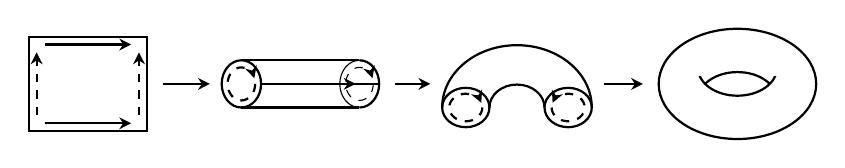
\begin{tikzpicture}
        \begin{scope}
            \draw[thick] (0,0) rectangle (1.5,1.2);
            \draw[-{Stealth[length=1.5mm, width=1.5mm]},thick, dashed] (0.1,0.2)--(0.1,1.0);
            \draw[-{Stealth[length=1.5mm, width=1.5mm]},thick, dashed] (1.4,0.2)--(1.4,1.0);
            \draw[-{Stealth[length=1.5mm, width=1.5mm]},thick] (0.2,0.1)--(1.3,0.1);
            \draw[-{Stealth[length=1.5mm, width=1.5mm]},thick] (0.2,1.1) -- (1.3,1.1);
        \end{scope}
        \begin{scope}[xshift=2.7cm, yshift=0.6cm]
            \pgfmathsetmacro{\smallradius}{0.25}
            \pgfmathsetmacro{\largeradius}{0.3}
            \pgfmathsetmacro{\cylinderlength}{1.5}
            \pgfmathsetmacro{\arrowthreshold}{0.3}
            \draw[thick] (0,0) ellipse ({\smallradius} and {\largeradius});

            \draw[-{Stealth[length=1.5mm, width=1.5mm]}, thick, dashed] ({\smallradius*(1-\arrowthreshold)},0) arc (360:20:{\smallradius*(1-\arrowthreshold)} and {\largeradius*(1-\arrowthreshold)});
            \draw[-{Stealth[length=1.5mm, width=1.5mm]}, dashed] ({\smallradius*(1-\arrowthreshold)+\cylinderlength},0) arc (360:20:{\smallradius*(1-\arrowthreshold)} and {\largeradius*(1-\arrowthreshold)});

            \draw[thick] (0,-\largeradius) -- (\cylinderlength,-\largeradius);
            \draw[thick] (0,\largeradius) -- (\cylinderlength,\largeradius);
            \draw[thick] (\smallradius,0) -- (\smallradius + \cylinderlength,0);

            \draw (\cylinderlength,-\largeradius) arc (270:90:{\smallradius} and {\largeradius});
            \draw[thick] (\cylinderlength,\largeradius) arc (90:-90:{\smallradius} and {\largeradius});

            \draw[-{Stealth[length=1.5mm, width=1.5mm]}] (\smallradius+\arrowthreshold, 0)--(\cylinderlength+\smallradius-\arrowthreshold, 0);
        \end{scope}
        \begin{scope}[xshift=6.2cm, yshift=0.3cm]
            \pgfmathsetmacro{\smallradius}{0.25}
            \pgfmathsetmacro{\largeradius}{0.3}
            \pgfmathsetmacro{\halfcenterdistance}{0.65}
            \pgfmathsetmacro{\arrowthreshold}{0.3}

            \draw[thick] (-\halfcenterdistance,0) ellipse ({\largeradius} and {\smallradius});
            \draw[thick] (\halfcenterdistance,0) ellipse ({\largeradius} and {\smallradius});

            \draw[-{Stealth[length=1.5mm, width=1.5mm]}, thick, dashed] ({-\halfcenterdistance+\largeradius*(1-\arrowthreshold)},0) arc (360:20:{\largeradius*(1-\arrowthreshold)} and {\smallradius*(1-\arrowthreshold)});

            \draw[-{Stealth[length=1.5mm, width=1.5mm]}, thick, dashed] ({\halfcenterdistance-\largeradius*(1-\arrowthreshold)},0) arc (-180:160:{\largeradius*(1-\arrowthreshold)} and {\smallradius*(1-\arrowthreshold)});

            \draw[thick] (\halfcenterdistance-\largeradius,0) arc (0:180:{\halfcenterdistance-\largeradius} and {(\halfcenterdistance-\largeradius)*\smallradius/\largeradius});
            \draw[thick] (\halfcenterdistance+\largeradius,0) arc (0:180:{\halfcenterdistance+\largeradius} and {(\halfcenterdistance+\largeradius)*\smallradius/\largeradius});
        \end{scope}
        \begin{scope}[xshift=9cm, yshift=0.6cm]
            \pgfmathsetmacro{\smallradius}{0.25}
            \pgfmathsetmacro{\largeradius}{0.3}

            \draw[thick] (0,0) ellipse (1 and 0.7);
            \begin{scope}
                \clip (-0.6,0) rectangle (0.6,0.4);
                \draw[thick] (-0.5,-0.2) arc (180:0:{0.5} and {0.5*0.7});
            \end{scope}
            \begin{scope}
                \clip (-0.6,0.1) rectangle (0.6,-0.3);
                \draw[thick] (-0.5,0.2) arc (180:360:{0.5} and {0.5*0.7});
            \end{scope}
        \end{scope}
        \draw[-{Stealth[length=1.5mm, width=1.5mm]}, thick] (1.7,0.6) -- (2.3,0.6);
        \draw[-{Stealth[length=1.5mm, width=1.5mm]}, thick] (4.65,0.6) -- (5.1,0.6);
        \draw[-{Stealth[length=1.5mm, width=1.5mm]}, thick] (7.3,0.6) -- (7.8,0.6);
    \end{tikzpicture}
    \caption{Illustration of the deformation of a homeomorphism between a rectangle with opposite sides \textit{identified} and a torus.}\label{fig:identifiedrectagletotorushomeomorphism}
\end{figure}The properties of an elliptic function can be more easily observed on its fundamental parallelogram, since the values of \(f\) on \(\mathbb{C}\) are fully represented by its values on \(P\). Because the opposite sides of the parallelogram are \textscsl{identified} (treated to be the same, or topologically ``glued together'') by the periodicity of \(f\), the fundamental parallelogram is homeomorphic to a torus, as visualized in \cref{fig:identifiedrectagletotorushomeomorphism}.

Let \(\mathbb{C}\) be closed under addition and let \(\Lambda\) be the subgroup of \(\mathbb{C}\). Then, the quotient group \(\mathbb{C}/\Lambda\) is compact as it is homeomorphic to a torus, which is endowed with a compact topology. Hence, Liouville (\cref{thm:liouville}) implies that if \(f\) does not have poles, then it must be constant:
\begin{theorem}[Liouville]\label{thm:liouvilleelliptic}
    Any elliptic function \(f\) with period lattice \(\Lambda\) that is holomorphic on \(\mathbb{C}\) is constant.
\end{theorem}
\begin{proposition}
    The number of zeros and poles (counting multiplicities and orders) of a non-constant elliptic function \(f\) in \(\mathbb{C}/\Lambda\) is finite, where \(\Lambda\) is the period lattice of \(f\).
\end{proposition}
\begin{proof}
    Let \(P\) be a fundamental parallelogram of \(\Lambda\). It suffices to show that \(f\) has finitely many zeros and poles in \(\overline{P}\). If there are infinitely many poles in \(\overline{P}\), then by the Bolzano--Weierstrass Theorem (\cref{thm:bolzanoweierstrass}), there exists an accumulation point \(z_0\in\overline{P}\) of poles. Hence, \(z_0\) cannot be an isolated singularity, contradicting meromorphy (more succinctly, \(z_0\) is then an essential singularity on the Riemann sphere).

    Under the assumption that \(f\not\equiv 0\), the same argument shows that \(\frac{1}{f}\) has finitely many poles in \(\overline{P}\), or equivalently, that \(f\) has finitely many zeros in \(\overline{P}\).
\end{proof}
\begin{proposition}\label{prop:ellipticfunctionresiduesum}
    For any elliptic function \(f\) with period lattice \(\Lambda\), the sum of the residues of \(f\) in \(\mathbb{C}/\Lambda\) is zero.
\end{proposition}
\begin{proof}
    Let \(\alpha\), \(\alpha+\omega_1\), \(\alpha+\omega_2\), and \(\alpha+\omega_1+\omega_2\) be the vertices of a fundamental parallelogram \(P\) of \(\Lambda\) such that \(\partial P\) does not pass through the poles \(f\). By the Residue Theorem (\cref{thm:residuethm}), we have \[2\piup\ii\sum_{z_k\in P}\residue_{z=z_k}f(z)=\oint_{\partial P}f(z)\ddz,\] where the sum is over all poles \(z_k\) of \(f\) in \(\mathbb{C}/\Lambda\) (effectively \(P\)). The integral is equivalent to
    \begin{align*}
        \oint_{\partial P}f(z)\ddz&=\pm\qty(\int_\alpha^{\alpha+\omega_1}+\int_{\alpha+\omega_1}^{\alpha+\omega_1+\omega_2}+\int_{\alpha+\omega_1+\omega_2}^{\alpha+\omega_2}+\int_{\alpha+\omega_2}^\alpha)f(z)\ddz\\
        &=\pm\qty(\int_\alpha^{\alpha+\omega_1}+\int_{\alpha}^{\alpha+\omega_2}+\int_{\alpha+\omega_1}^{\alpha}+\int_{\alpha+\omega_2}^\alpha)f(z)\ddz=0
    \end{align*} by the periodicity of \(f\).
\end{proof}
\begin{theorem}\label{thm:ellipticfunctionnumberofzerosandpoles}
    For any non-constant elliptic function \(f\) with period lattice \(\Lambda\), the number of zeros and poles (counting multiplicities and orders, respectively) in \(\mathbb{C}/\Lambda\) are equal.
\end{theorem}
\begin{proof}
    Let \(P\) be a fundamental parallelogram of \(\Lambda\) such that \(\partial P\) \(f\) has no poles or zeros thereon. By the Argument Principle (\cref{thm:argumentprinciplemeromorphic}), we have \[\frac{1}{2\piup\ii}\oint_{\partial P}\frac{f'(z)}{f(z)}\ddz=\text{\# of zeros in \(P\)}-\text{\# of poles in \(P\)}\] where the sums are over all zeros and poles of \(f\) in \(\mathbb{C}/\Lambda\) (effectively \(P\)) counted with multiplicities and orders, respectively. By assumption, \(f'\not\equiv 0\), and hence \(\frac{f'}{f}\) is non-constant and elliptic with period lattice \(\Lambda\). By \cref{prop:ellipticfunctionresiduesum}, the integral vanishes and hence the assertion follows.
\end{proof}
\begin{proposition}
    Suppose \(f\) is a non-constant elliptic function with period lattice \(\Lambda\). Then \(f\) attains every value in \(\extcomplex\) the same number of times (counting multiplicities) in \(\mathbb{C}/\Lambda\).
\end{proposition}
\begin{proof}
    Assume that \(z\neq\infty\) and suppose \(P\) is a fundamental parallelogram that does not pass through a pole. Then the number of times \(\zeta\mapsto f(\zeta)-z\) attains \(0\) and \(\infty\) in \(\mathbb{C}/\Lambda\) are equal by \cref{thm:ellipticfunctionnumberofzerosandpoles}. In other words, \(f\) has the same number of poles as the number of times it attains any finite complex number.
\end{proof}
Hence, it is only natural to quantify this number:
\begin{definition}
    An elliptic function \(f\) is said to be of \textscsl{order} \(n\) iff it attains every value in \(\extcomplex\) exactly \(n\) times (counting multiplicities) in \(\mathbb{C}/\Lambda\), where \(\Lambda\) is the period lattice of \(f\) (in other words, the number of poles of \(f\) in a fundamental parallelogram, counted according to order, is \(n\)).
\end{definition}
\begin{proposition}
    A non-constant elliptic function \(f\) is of order \(\geq 2\).
\end{proposition}
\begin{proof}
    If \(f\) is of order 1, then \(f\) has a simple pole at some \(z_0\) in a fundamental parallelogram of its period lattice \(\Lambda\). By the simplicity of the pole, it must have a nonzero residue there. By \cref{prop:ellipticfunctionresiduesum}, this is an impossibility.
\end{proof}
\begin{theorem}
    Suppose that \(f\) is a non-constant elliptic function with period lattice \(\Lambda\). Let \(a_1,\ldots,a_n\) and \(b_1,\ldots,b_n\) be the zeros and poles (counting multiplicities and orders, respectively) in a fundamental parallelogram \(P\) (whose boundary intersects neither zeros or poles) of \(\Lambda\). Then \[\sum_{j=1}^n a_j-\sum_{j=1}^n b_j\in\Lambda,\] or in other words, this difference is also a period of \(f\).
\end{theorem}
\begin{proof}
    By \cref{thm:generalizedargumentprinciple}, the quantity in question is equal to
    \begin{align*}
        \sum_{j=1}^n a_j-\sum_{j=1}^n b_j&=\frac1{2\piup\ii}\oint_{\partial P}\frac{zf'(z)}{f(z)}\ddz\\
        &=\pm\frac1{2\piup\ii}\qty(\int_\alpha^{\alpha+\omega_1}+\int_{\alpha+\omega_1}^{\alpha+\omega_1+\omega_2}+\int_{\alpha+\omega_1+\omega_2}^{\alpha+\omega_2}+\int_{\alpha+\omega_2}^\alpha)\frac{zf'(z)}{f(z)}\ddz\\
        &=\pm\frac1{2\piup\ii}\qty(\int_\alpha^{\alpha+\omega_1}+\int_{\alpha+\omega_2}^\alpha)\frac{zf'(z)}{f(z)}\ddz\\
        &\quad\pm\frac{1}{2\piup\ii}\qty(\int_\alpha^{\alpha+\omega_2}\frac{\qty(z+\omega_1)f'(z)}{f(z)}\ddz+\int_{\alpha+\omega_1}^\alpha\frac{\qty(z+\omega_2)f'(z)}{f(z)}\ddz)\\
        &=\pm\frac1{2\piup\ii}\qty(\int_{\alpha+\omega_1}^\alpha\frac{\omega_2f'(z)}{f(z)}\ddz+\int_\alpha^{\alpha+\omega_2}\frac{\omega_1f'(z)}{f(z)}\ddz)c\\
        &=\pm\frac{\omega_2}{2\piup\ii}\qty(\log{f(\alpha)}-\log{f\qty(\alpha+\omega_1)})\pm\frac{\omega_1}{2\piup\ii}\qty(\log{f\qty(\alpha+\omega_2)}-\log{f\qty(\alpha)})\\
        &=\pm\frac{\omega_2}{2\piup\ii}\log(1)\pm\frac{\omega_1}{2\piup\ii}\log(1).
    \end{align*}
    Since the branches of the multi-valued logarithm differ by integer multiples of \(2\piup\ii\), the assertion follows.
\end{proof}
\subsubsection{Weierstrass Elliptic Functions}
Since any non-constant elliptic function has order greater than one, it is natural to next consider elliptic functions of order two.

Within a fundamental parallelogram, by \cref{thm:ellipticfunctionnumberofzerosandpoles}, such a function either has two simple poles or a single double pole. This distinction is the key difference between the Weierstrass theory of elliptic functions (the former case) and the Jacobi theory (the latter case).

In practice, elliptic functions derived from the Jacobi formulation often have more practical use cases, whereas the Weierstrass theory tends to be more convenient in theoretical analysis.
\begin{proposition}\label{prop:weierstrasspfunctionintermediateseriesconvergence}
    Let \(\omega_1\), \(\omega_2\) be a fundamental pair of periods generating the lattice \(\Lambda\). Then the series
    \begin{equation}
        \sum_{\omega\in\Lambda\setminus\qty{0}}\frac{1}{\abs{\omega}^\alpha}\label{eq:weierstrasspfunctionintermediateseriesconvergence_statement}
    \end{equation} is (absolutely) convergent for \(\alpha>2\).
\end{proposition}
\begin{proof}
    \begin{figure}
        \centering
        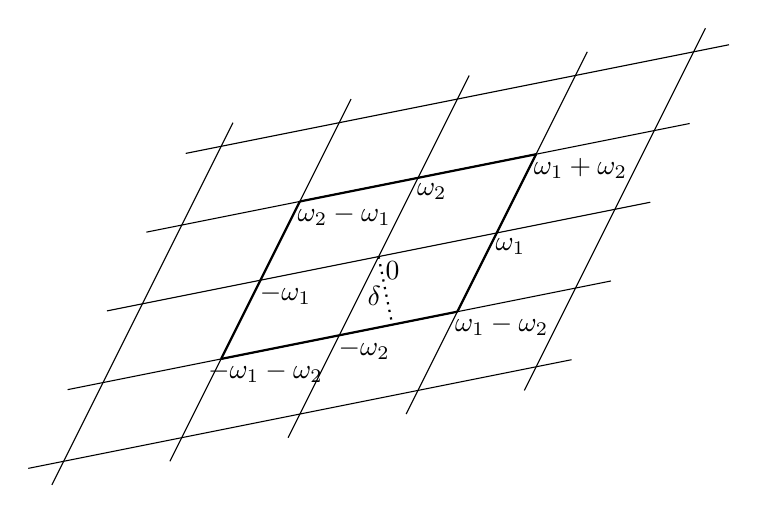
\begin{tikzpicture}
            \pgfmathsetmacro{\n}{4}
            \pgfmathsetmacro{\ax}{1.5}
            \pgfmathsetmacro{\ay}{0.3}
            \pgfmathsetmacro{\bx}{0.5}
            \pgfmathsetmacro{\by}{1.0}
            \pgfmathsetmacro{\over}{0.3}
            \foreach \j in {0,...,\n} {
                \draw[thin]
                ({-\over*\ax+\j*\bx},{-\over*\ay+\j*\by})
                -- ({(\n+\over)*\ax+\j*\bx},{(\n+\over)*\ay+\j*\by});
            }
            \foreach \i in {0,...,\n} {
                \draw[thin]
                ({-\over*\bx+\i*\ax},{-\over*\by+\i*\ay}) -- ({\i*\ax+(\n+\over)*\bx},{\i*\ay+(\n+\over)*\by});
            }
            \foreach \i in {-1,1} {
                \draw[thick] ({\ax*(\n/2+\i)+\bx*(\n/2-1)},{\ay*(\n/2+\i)+\by*(\n/2-1)}) -- ({\ax*(\n/2+\i)+\bx*(\n/2+1)},{\ay*(\n/2+\i)+\by*(\n/2+1)});
                \draw[thick] ({\ax*(\n/2-1)+\bx*(\n/2+\i)},{\ay*(\n/2-1)+\by*(\n/2+\i)}) -- ({\ax*(\n/2+1)+\bx*(\n/2+\i)},{\ay*(\n/2+1)+\by*(\n/2+\i)});
            }
            \node[shift={(5pt,-5pt)}] at ({\ax*(\n/2)+\bx*(\n/2)},{\ay*(\n/2)+\by*(\n/2)}) {\(0\)};
            \node[shift={(5pt,-5pt)}] at ({\ax*(\n/2+1)+\bx*(\n/2)},{\ay*(\n/2+1)+\by*(\n/2)}) {\(\omega_1\)};
            \node[shift={(9pt,-5pt)}] at ({\ax*(\n/2-1)+\bx*(\n/2)},{\ay*(\n/2-1)+\by*(\n/2)}) {\(-\omega_1\)};
            \node[shift={(5pt,-5pt)}] at ({\ax*(\n/2)+\bx*(\n/2+1)},{\ay*(\n/2)+\by*(\n/2+1)}) {\(\omega_2\)};
            \node[shift={(9pt,-5pt)}] at ({\ax*(\n/2)+\bx*(\n/2-1)},{\ay*(\n/2)+\by*(\n/2-1)}) {\(-\omega_2\)};
            \node[shift={(16pt,-5pt)}] at ({\ax*(\n/2+1)+\bx*(\n/2+1)},{\ay*(\n/2+1)+\by*(\n/2+1)}) {\(\omega_1+\omega_2\)};
            \node[shift={(16pt,-5pt)}] at ({\ax*(\n/2-1)+\bx*(\n/2-1)},{\ay*(\n/2-1)+\by*(\n/2-1)}) {\(-\omega_1-\omega_2\)};
            \node[shift={(16pt,-5pt)}] at ({\ax*(\n/2-1)+\bx*(\n/2+1)},{\ay*(\n/2-1)+\by*(\n/2+1)}) {\(\omega_2-\omega_1\)};
            \node[shift={(16pt,-5pt)}] at ({\ax*(\n/2+1)+\bx*(\n/2-1)},{\ay*(\n/2+1)+\by*(\n/2-1)}) {\(\omega_1-\omega_2\)};
            \coordinate (O) at ({\ax*(\n/2)+\bx*(\n/2)},{\ay*(\n/2)+\by*(\n/2)});

            \pgfmathsetmacro{\lengtha}{sqrt(\ax*\ax+\ay*\ay)}
            \pgfmathsetmacro{\lengthb}{sqrt(\bx*\bx+\by*\by)}
            \pgfmathsetmacro{\sineanglebetween}{sqrt(1-((\ax*\bx+\ay*\by)/(\lengtha*\lengthb))^2)}
            \coordinate (H) at ([shift={(\ay*\lengthb*\sineanglebetween/\lengtha,-\ax*\lengthb*\sineanglebetween/\lengtha)}] O);
            \draw[dotted, thick] (O) -- (H);
            \node[xshift=-4, yshift=-2] at ($(O)!0.5!(H)$) {\(\delta\)};
        \end{tikzpicture}
        \caption{The parallelogram \(P_1\) with 8 periods on its boundary with lattice \(\Lambda\).}\label{fig:weierstrasspfunctionintermediateseriesconvergence_parallelogram}
    \end{figure}Let \(P_n\) be a parallelogram whose center is 0 and has \(n\qty(\omega_1+\omega_2)\) as a vertex (the specific case of \(n=1\) is illustrated in \cref{fig:weierstrasspfunctionintermediateseriesconvergence_parallelogram}). For each \(n\in\mathbb{N}\), there exist \(8n\) periods (points in \(\Lambda\)) on \(\partial P_n\).

    Let \(\delta\) be the distance from 0 to \(\partial P_1\). Hence, the distance from 0 to \(\partial P_n\) is \(n\delta\). Since each \(\omega\in\Lambda^*=\Lambda\setminus\qty{0}\) lies in a unique \(\partial P_n\), it follows that \(\abs{\omega}^\alpha\geq n^\alpha \delta^\alpha\) for all \(\alpha>0\). Hence, \[\sum_{\omega\in\Lambda^*}\frac{1}{\abs{\omega}^\alpha}\leq\sum_{n=1}^\infty\frac{8n}{n^\alpha\delta^\alpha}=\frac{8}{\delta^\alpha}\sum_{n=1}^\infty\frac{1}{n^{\alpha-1}},\] which is a \(p\)-series that converges for \(\alpha>2\).
\end{proof}
\begin{proposition}\label{prop:weierstrasspfunctionconvergence}
    Let \(\omega_1\), \(\omega_2\) be a fundamental pair of periods generating the lattice \(\Lambda\). Then the series
    \begin{equation}
        \sum_{\omega\in\Lambda\setminus\qty{0}}\qty[\frac{1}{\qty(z-\omega)^2}-\frac{1}{\omega^2}]\label{eq:weierstrasspfunctionconvergence_statement}
    \end{equation}
    locally uniformly converges on \(\mathbb{C}\setminus\Lambda\).
\end{proposition}
\begin{proof}
    Let \(R>0\) be arbitrary. Then \(\forall z\in D(0,R)\), and for \(\abs{\omega}>2R\), we have \[\frac{\abs{z}}{\abs{\omega}}<\frac12,\quad\abs{2-\frac{z}{\omega}}\leq 2+\frac{\abs{z}}{\abs{\omega}}<\frac52,\quad\abs{1-\frac{z}{\omega}}^2\geq\qty(1-\abs{\frac{z}{\omega}})^2>\frac14.\]
    It follows that
    \[\abs{\frac{1}{\qty(z-\omega)^2}-\frac{1}{\omega^2}}=\abs{\frac{2\omega z-z^2}{\omega^2(z-\omega)^2}}=\abs{\frac{z\qty(2-\frac{z}{\omega})}{\omega^3\qty(\frac{z}{\omega}-1)^2}}<\frac{\frac52z}{\frac14\omega^3}\leq\frac{10R}{\omega^3}.\]
    Hence, by \cref{prop:weierstrasspfunctionintermediateseriesconvergence},
    \begin{equation}
        \sum_{\substack{\omega\in\Lambda\\
        \omega\notin\overline{D\qty(0,2R)}}}\qty[\frac{1}{\qty(z-\omega)^2}-\frac{1}{\omega^2}]\label{eq:weierstrasspfunctionconvergence_intermediateseries}
    \end{equation} is termwise bounded by a series \(\sum_{\substack{\omega\in\Lambda\\
    \omega\notin\overline{D\qty(0,2R)}}}\frac{10R}{\omega^3}\), which is convergent by \cref{prop:weierstrasspfunctionintermediateseriesconvergence}. Weierstrass \(M\)--Test (\cref{thm:weierstrassmtest}) gives the uniform convergence of \cref{eq:weierstrasspfunctionconvergence_intermediateseries} on \(D(0,R)\). Since we have omitted only finitely many terms, \cref{eq:weierstrasspfunctionintermediateseriesconvergence_statement} converges uniformly on \(D(0,R)\setminus\Lambda\).

    Let \(K\subset\mathbb{C}\setminus\Lambda\) be compact and arbitrary. By boundedness, \(\exists R>0\) such that \(K\subset D(0,R)\setminus\Lambda\), on which it uniformly converges.
\end{proof}
\begin{definition}[Weierstrass \texorpdfstring{\(\wp\)}{p}-Function]\label{def:weierstrasspfunction}
    Let \(\omega_1\), \(\omega_2\) be a fundamental pair of periods generating the lattice \(\Lambda\). The Weierstrass \(\wp\)-function with period lattice \(\Lambda\) is defined by
    \begin{equation}
        \wp(z)=\frac{1}{z^2}+\sum_{\omega\in\Lambda\setminus\qty{0}}\qty[\frac{1}{\qty(z-\omega)^2}-\frac{1}{\omega^2}],\qquad z\in\mathbb{C}\setminus\Lambda.\label{eq:weierstrasspfunction}
    \end{equation}
\end{definition}
By \cref{prop:weierstrasspfunctionconvergence,thm:weierstrassconvergence}, \(\wp\) is well-defined and meromorphic on \(\mathbb{C}\). By \cref{thm:weierstrassconvergence}, we can use termwise differentiation to get \[\wp'(z)=-\frac{2}{z^3}-\sum_{\omega\in\Lambda\setminus\qty{0}}\frac{2}{\qty(z-\omega)^3}=-2\sum_{\omega\in\Lambda}\frac1{\qty(z-\omega)^3},\] which is absolutely convergent for \(z\notin\Lambda\). It follows that \(\wp'\) is also meromorphic on \(\mathbb{C}\). Hence, the series expression for \(\wp'(z)\) may be rearranged to \(\wp'(z+\omega_1)\), and hence, \[\wp'(z)=\wp'(z+\omega_1)=\wp'(z+\omega_2).\] Hence, \(\wp'\) is also an elliptic function with period lattice \(\Lambda\). Hence, we must have \[\wp(z)+c_1=\wp\qty(z+\omega_1),\qquad \wp(z)+c_2=\wp\qty(z+\omega_2).\] At \(z=-\frac{\omega_1}{2},-\frac{\omega_2}{2}\), we have \[\wp\qty(-\frac{\omega_1}{2})+c_1=\wp\qty(\frac{\omega_1}{2}),\qquad\wp\qty(-\frac{\omega_2}{2})+c_2=\wp\qty(\frac{\omega_2}{2})\] By evenness of \(\wp\), we must have \(c_1=c_2=0\). Therefore, \(\wp\) is also an elliptic function with period lattice \(\Lambda\). Moreover, each isolated singularity \(\omega\in\Lambda\) is a pole of order two with residue 0 (by \cref{prop:ellipticfunctionresiduesum}). The quotient group \(\mathbb{C}/\Lambda\), may be represented by a fundamental parallelogram \(P\) of \(\Lambda\) with vertices at \(0\), \(\omega_1\), \(\omega_2\), and \(\omega_1+\omega_2\), which by identification, are homeomorphic to a single point on the torus.


\begin{definition}[Weierstrass \(\zeta\)-Function]

\end{definition}
\begin{definition}[Weierstrass \(\sigma\)-Function]

\end{definition}
\subsubsection{Jacobi Elliptic Functions}
\newcommand{\sn}{\operatorname{sn}}
\newcommand{\cn}{\operatorname{cn}}
\newcommand{\dn}{\operatorname{dn}}
\subsubsection{The Modular Group}
Any two bases of
\subsection{Schlicht Functions}
\begin{theorem}[\textsc{Koebe Quarter Theorem}]\label{thm:koebequarter}

\end{theorem}
\subsubsection{The Bieberbach Conjecture}
\subsection{Boundary Continuity of Biholomorphisms}
Suppose \(\Omega_1\) and \(\Omega_2\) are two regions in the complex plane such that there is a biholomorphism \(\varphi\) from \(\Omega_1\) to \(\Omega_2\). Naturally, we are concerned about the existence of a continuous extension of \(\varphi\) to \(\overline{\Omega_1}\).

As a matter of fact, it is almost always true that such an extension exists. We will give three dominant scenarios:
\begin{enumerate}
    \item If \(\partial\Omega_1\) and \(\partial\Omega_2\) are two Jordan curves, then \(\varphi\) (whose existence is given by the Riemann Mapping Theorem or \cref{thm:riemannmapping}) extends injectively and continuously to \(\partial\Omega_1\).
    \item
\end{enumerate}
The first result is given by:
\begin{theorem}[\textsc{Osgood--Taylor--Carathéodory}]\label{thm:osgoodtaylorcaratheodory}

\end{theorem}
\section{The Prime Number Theorem}
The Riemann \(\zeta\)-function is one of the most important functions in analytic number theory due to its connection with the distribution of prime numbers. We will also introduce one of the most profound theorems in number theory on the distribution of prime numbers.
\subsection{The \texorpdfstring{\(\Gamma\)}{Gamma} Function}\label{sec:gammafunction}
\begin{definition}\label{def:gammafunction}
    The Gamma function is defined by
    \begin{equation}
        \Gamma(z)=\int_0^\infty \ee^{-t}t^{z-1}\dd{t},\label{eq:gammafunction}
    \end{equation} where \(z\in\mathbb{C}\).
\end{definition}
By letting \(z=x+\ii y\) where \(x,y\in\mathbb{R}\), we have \(\abs{\ee^{-t}t^{z-1}}=\ee^{-t}t^{x-1}\). Notice that for \(x>0\),
\begin{align*}
    \abs{\Gamma(x)} & =\int_0^1 \ee^{-t}t^{x-1}\ddt+\int_1^\infty \ee^{-t}t^{x-1}\ddt \\
    & \leq\int_0^1 t^{x-1}\ddt+\int_1^\infty \ee^{-t}t^{x-1}\ddt      \\
    & =\frac{1}{x}+\int_1^\infty \ee^{-t}t^{x-1}\ddt.
\end{align*}
Since \(\int_1^\infty\frac{\ddt}{t^2}\) is convergent and \(\lim_{t\to\infty}\frac{\ee^{-t}t^{z-1}}{t^{-2}}=0\), then by comparison, the second integral is convergent.

Therefore, \(\Gamma(x)\) is convergent on \(\mathbb{R}_{>0}\). It follows that \(\Gamma(z)\) is absolutely convergent on the right half-plane \(\cbraces{z\in\mathbb{C}}{\Re(z)>0}\). Furthermore, \(\Gamma(z)\) is well-defined and holomorphic on \(\cbraces{z\in\mathbb{C}}{\Re(z)>0}\). From integration by parts, we get
\begin{align*}
    \Gamma(z+1) & =\int_0^\infty \ee^{-t}t^z\ddt                                   \\
    & =-\eval{\ee^{-t}t^z}_0^\infty+z\int_0^\infty\ee^{-t}t^{z-1}\ddt. \\
    & =z\Gamma(z).
\end{align*}
Additionally, \[\Gamma(1)=\int_0^\infty \ee^{-t}\ddt=-\eval{\ee^{-t}}_0^\infty=1.\]
Hence, we have \(\Gamma(z+1)=z!\), and the \(\Gamma\) function generalizes the factorial. We also have \[\Gamma(z+n)=\Gamma(z)\prod_{k=0}^{n-1}(z+k),\quad\Re(z)>0, n\in\mathbb{N}.\]
Therefore, can derive its analytic continuation via
\[\Gamma(z)=\frac{\Gamma(z+n)}{\prod_{k=0}^{n-1}(z+k)},\quad\Re(z)>-n.\]
Since the numerator is holomorphic on \(\Re(z)>-n\) and \(n\) was arbitrary, the analytic continuation of \(\Gamma\) has simple poles at each of \(\mathbb{Z}_{\leq0}\). Hence, \(\Gamma(z)\) is meromorphic on \(\mathbb{C}\).

By \cref{eq:residueatpole}, the residue at each pole is equal to
\[\residue_{z=-n}\Gamma(z)=\lim_{z\to -n}\frac{\Gamma(z+n+1)}{\prod_{k=0}^{n-1}(z+k)}=\frac{1}{\prod_{k=1}^n(-k)}=\frac{{(-1)}^n}{n!}.\]
We will now study two representations for the Gamma function.
\begin{theorem}[Gauss]\label{thm:gammafunctiongaussformula}
    The Gamma function satisfies
    \begin{equation}
        \Gamma(z)=\lim_{n\to\infty}\frac{n^z n!}{\prod_{k=0}^n (z+k)}\label{eq:gammafunctiongaussformula}
    \end{equation}
    for \(\Re(z)>0\).
\end{theorem}
\begin{proof}
    \[f_n(z)=\int_0^n{\qty(1-\frac{t}{n})}^n t^{z-1}\ddt=n^z\int_0^1{\qty(1-t)}^n t^{z-1}\ddt,\quad\Re(z)>0.\]
    By integration by parts, we have
    \begin{align}
        f_n(z) & =n^z\qty[\eval{\frac{t^z}{z}{(1-t)}^n}_0^1+\frac{n}{z}\int_0^1{(1-t)}^{n-1}t^z \ddt]                                     \nonumber \\
        & =\qty(\frac{n}{n-1})^{z+1}\frac{f_{n-1}\qty(z+1)}{z}=\qty[\frac{n^{z+1}(n-1)}{{(n-2)}^{z+2}}]\frac{f_{n-2}(z+2)}{z(z+1)} \nonumber \\
        & =n^{z+1}(n-1)!\frac{f_1(z+n-1)}{\prod_{k=0}^{n-2}(z+k)}                                                                  \nonumber \\
        & =\frac{n^z n!}{\prod_{k=0}^n(z+k)}.\label{eq:gammafunctiongaussformulaprelimit}
    \end{align}
    Let us now analyze the difference
    \begin{equation}
        \lim_{n\to\infty}\qty[\int_0^n \ee^{-t}t^{z-1}\ddt-f_n(z)]=\lim_{n\to\infty}\int_0^n \ee^{-t}t^{z-1}\qty[1-\ee^{t}{\qty(1-\frac{t}{n})}^n]\ddt.\label{eq:gammafunction_gaussformulaintermediate1}
    \end{equation}
    Since \[\dv{t}(\ee^t{\qty(1-\frac{t}{n})}^n)=\ee^t
    \qty(1-\frac{t}{n})^n-\ee^t\qty(1-\frac{t}{n})^{n-1}=-\ee^t\frac{t}{n}{\qty(1-\frac{t}{n})}^{n-1},\]
    we have
    \begin{equation}
        1-\ee^t\qty(1-\frac{t}{n})^n=\frac{1}{n}\int_0^t u\ee^u\qty(1-\frac{u}{n})^{n-1}\dd{u}.\label{eq:gammafunction_gaussformulaintermediate2}
    \end{equation}
    Additionally, since
    \begin{align*}
        \dv{u}(\ee^u\qty(1-\frac{u}{n})^{n-1}) & =\ee^u\qty(1-\frac{u}{n})^{n-1}-\frac{n-1}{n}\ee^u\qty(1-\frac{u}{n})^{n-2} \\
        & =\frac{\ee^u}{n}\qty(1-\frac{u}{n})^{n-2}\qty(1-u)
    \end{align*} has zeros at \(u=1\) and at \(u=n\), and \[\dv[2]{u}(\ee^u\qty(1-\frac{u}{n})^{n-1})=\frac{\ee^u}{n^2}\qty(1-\frac{u}{n})^{n-3}\qty(u^{2}-2u-n+2),\]
    which evaluates to \(-\frac{\ee(n-1)^{n-2}}{n^{n-1}}<0\) at \(u=1\) and evaluates to \[\frac{\ee^n}{n^{n-1}}\qty(n-u)^{n-3}(n-2)(n-1)\to0^+\] as \(u\to n^-\). Therefore, \(\ee^u{\qty(1-\frac{u}{n})}^{n-1}\) attains its maximum of \(\ee{\qty(\frac{n-1}{n})}^{n-1}\) at \(u=1\). For \(n>1\), \(\ee\qty(\frac{n-1}{n})^{n-1}\leq \ee\). From \cref{eq:gammafunction_gaussformulaintermediate2}, we have \[1-\ee^{t}\qty(1-\frac{t}{n})^n\leq\frac{et^2}{2n}.\] Moreover, since for \(0\leq u\leq t\leq n\), \[u\ee^u\qty(1-\frac{u}{n})^{n-1}>0,\]
    it follows that \(1-\ee^{t}{\qty(1-\frac{t}{n})}^n\) is positive. By \cref{eq:gammafunction_gaussformulaintermediate1}, we have \[\abs{\int_0^n \ee^{-t}t^{z-1}\qty[1-\ee^{t}{\qty(1-\frac{t}{n})}^n]\ddt}\leq\frac{\ee}{2n}\abs{\int_0^n\ee^{-t}t^{z+1}\ddt}<\frac{1}{2n}\abs{\Gamma(z+2)}\to 0\] as \(n\to\infty\). From \cref{eq:gammafunctiongaussformulaprelimit}, we have \(\Gamma(z)=\lim_{n\to\infty}\frac{n^z n!}{\prod_{k=0}^n\qty(z+k)}\), or \cref{eq:gammafunctiongaussformula}
\end{proof}
The \textscsl{Weierstrass formula} is a direct consequence of the Gauss formula.
\begin{theorem}[Weierstrass]\label{thm:gammafunction_weierstrassformula}
    The reciprocal Gamma function has the entire Weierstrass factorization of
    \begin{equation}
        \frac{1}{\Gamma(z)}=z\prod_{k=1}^n\qty[\qty(1+\frac{z}{k})\ee^{-\frac{z}{k}}]\exp\qty(z\gamma).\label{eq:gammafunction_weierstrassformula}
    \end{equation}
\end{theorem}
\begin{proof}
    Since the Gauss formula agrees with \cref{eq:gammafunction} on the right half-plane, the analytic continuation of \(\Gamma(z)\) is unique on the entire complex plane except for the poles at \(\mathbb{Z}_{\leq0}\) by the Identity Theorem (\cref{thm:identity}). Since
    \begin{align*}
        \frac{n^z n!}{\prod_{k=0}^n\qty(z+k)} & =\frac{\exp\qty[z\log(n)]}{z\prod_{k=1}^n \qty(1+\frac{z}{k})}                                                                                                 \\
        & =\frac{\exp\qty[z\int_1^n\frac{1}{x}\ddx]}{z\prod_{k=1}^n \qty(1+\frac{z}{k})}\frac{\exp\qty[-z\sum_{k=1}^n\frac{1}{k}]}{\prod_{k=1}^n\exp\qty[-\frac{z}{k}]} \\
        & =\frac{1}{z\prod_{k=1}^n\qty[\qty(1+\frac{z}{k})\ee^{-\frac{z}{k}}]}\exp\qty[-z\qty(\int_1^n\qty(\frac{1}{\floor{x}}-\frac{1}{x})\ddx)].
    \end{align*}
    Therefore,
    \begin{align*}
        \frac{1}{\Gamma(z)} & =\lim_{n\to\infty}\frac{\prod_{k=0}^n(z+k)}{n^z n!}                                                                                           \\
        & =z\prod_{k=1}^n\qty[\qty(1+\frac{z}{k})\ee^{-\frac{z}{k}}]\lim_{n\to\infty}\exp\qty[z\qty(\int_1^n\qty(\frac{1}{\floor{x}}-\frac{1}{x})\ddx)] \\
        & =z\prod_{k=1}^n\qty[\qty(1+\frac{z}{k})\ee^{-\frac{z}{k}}]\exp\qty(z\gammaup).
    \end{align*}
    The constant \(\gammaup=\int_1^\infty\qty(\frac{1}{\floor{x}}-\frac{1}{x})\ddx\) is known as the \textscsl{Euler--Mascheroni constant}. By the Weierstrass Factorization Theorem (\cref{thm:weierstrassfactorization}), if we let \(a_n=-n\) and \(p_n=1\), it follows that \[\sum_{n=1}^\infty\abs{\frac{R}{a_n}}^{p_n+1}=R^2\sum_{n=1}^\infty\frac{1}{n^2}=\frac{R^2\piup^2}{6}\] is convergent. Thus, the Weierstrass formula defines an entire function with zeros at each of \(\mathbb{Z}_{\leq 0}\).
\end{proof}
We have two famous identities on the \(\Gamma\) function:
\begin{theorem}[Euler's Reflection Formula]\label{thm:gammafunction_eulerreflection}
    The analytic continuation of the \(\Gamma\) function can be analytically continued to the left half-plane with the functional equation of
    \begin{equation}
        \Gamma(z)\Gamma(1-z)=\piup\csc(\piup z)\label{eq:gammafunction_eulerreflection}
    \end{equation} for \(z\in\mathbb{C}\setminus\mathbb{N}\).
\end{theorem}
\begin{proof}
    By the Weierstrass Formula (\cref{thm:gammafunction_weierstrassformula}), we have
    \begin{align*}
        \frac{1}{\Gamma(z)} & =z\prod_{k=1}^n\qty[\qty(1+\frac{z}{k})\ee^{-\frac{z}{k}}]\exp\qty(z\gammaup), \\\frac{1}{\Gamma(-z)}&=-z\prod_{k=1}^n\qty[\qty(1-\frac{z}{k})\ee^{\frac{z}{k}}]\exp\qty(-z\gammaup).
    \end{align*}
    Since the Weierstrass elementary factors form an absolutely convergent infinite product, we may rearrange its terms. Hence, by \cref{ex:sinproductformula}, we have \[\frac{1}{\Gamma(z)\Gamma(1-z)}=-\frac{1}{z\Gamma(z)\Gamma(-z)}=z\prod_{k=1}^n\qty(1-\frac{z^2}{k^2})=\frac{\sin(\piup z)}{\piup},\] which confirms \cref{eq:gammafunction_eulerreflection}.
\end{proof}
\begin{example}\label{ex:gammafunction_onehalf}
    Evaluate \(\Gamma\qty(\frac{1}{2})\).
\end{example}
\begin{proof}
    By the Reflection Formula (\cref{thm:gammafunction_eulerreflection}), we have that \[\Gamma\qty(\frac{1}{2})^2=\piup\csc(\frac{\piup}{2})=\piup,\]
    and it follows that \(\Gamma\qty(\frac{1}{2})=\sqrt{\piup}\) as it is positive.
\end{proof}
\begin{theorem}[Legendre's Duplication Formula]\label{thm:gammafunction_legendreduplication}
    For any \(z\in\mathbb{C}\setminus\qty(-\frac{\mathbb{N}}{2})\), we have
    \begin{equation}
        \Gamma(z)\Gamma\qty(z+\frac{1}{2})=2^{1-2z}\sqrt{\piup}\Gamma(2z).\label{eq:gammafunction_legendreduplication}
    \end{equation}
\end{theorem}
\begin{proof}
    From \cref{thm:gammafunctiongaussformula}, we have \[\Gamma(z)\Gamma\qty(z+\frac{1}{2})=\lim_{n\to\infty}\frac{n^{2z+\frac{1}{2}}n!^2}{\prod_{k=0}^n(z+k)\qty(z+k+\frac{1}{2})}=\lim_{n\to\infty}\frac{2^{2n+2}n^{2z+\frac{1}{2}}n!^2}{\prod_{k=0}^{2n+1}(2z+k)}\]
    where the left-hand side is defined since \(z\in\mathbb{C}\setminus\qty(-\frac{\mathbb{N}}{2})\).
    By expansion of the value, we have
    \begin{align*}
        \Gamma(z)\Gamma\qty(z+\frac{1}{2}) & =\lim_{n\to\infty}\frac{\qty(2n)^{2z}(2n)!}{\prod_{k=0}^{2n}(2z+k)}\cdot\frac{n^{\frac{1}{2}}n!^2 2^{2n+2-2z}}{\qty(2z+2n+1)(2n)!} \\
        & =\Gamma(2z)\lim_{n\to\infty}\frac{n^{\frac{1}{2}}n!^2 2^{2-2z}}{(2z+2n+1)\prod_{k=0}^{n-1}\qty(k+\frac{1}{2})\prod_{k=1}^n k}      \\
        & =2^{2-2z}\Gamma(2z)\lim_{n\to\infty}\frac{n^{\frac{1}{2}}n!}{\prod_{k=0}^n\qty(k+\frac{1}{2})}\cdot\frac{n}{2z+2n+1}               \\
        & =2^{1-2z}\Gamma(2z)\Gamma\qty(\frac{1}{2})                                                                                         \\
        & =2^{1-2z}\Gamma(2z)\sqrt{\piup},
    \end{align*}
    where the last step is derived from \cref{ex:gammafunction_onehalf}.
\end{proof}
The identity above is a special case of the following result:
\begin{theorem}[Gauss Multiplication Theorem]
    Suppose \(m\in\mathbb{N}_{\geq 2}\). Let \(z\in\mathbb{C}\setminus\qty(-\frac{\mathbb{N}}{m})\). Then we have
    \begin{equation}
        \Gamma(z)\Gamma\qty(z+\frac{1}{m})\cdots\Gamma\qty(z+\frac{m-1}{m})=\qty(2\piup)^{\frac{m-1}{2}}m^{\frac{1}{2}-mz}\Gamma(mz).\label{eq:gammafunction_gaussmultiplication}
    \end{equation}
\end{theorem}
The Gamma function as in \cref{eq:gammafunction} is commonly referred to as the \textscsl{Euler Integral of the Second Kind}. The \textscsl{Euler Integral of the First Kind} is also known as the \textscsl{Beta function}, and is defined by \[\operatorname{B}\qty(z_1,z_2)=\int_0^1 t^{z_1-1}(1-t)^{z_2-1}\ddt.\] By a change of variables (by letting \(\tau=1-t\)), we derive the symmetry of the Beta function: \[\operatorname{B}\qty(z_1,z_2)=\int_0^1 \tau^{z_2-1}(1-\tau)^{z_1-1}\dd\tau=\operatorname{B}\qty(z_2,z_1).\]
The Beta function is commonly treated as an auxiliary function in many cases of integral evaluation due to its connection with the Gamma function:
\begin{theorem}\label{thm:betagammafunctionrelationship}
    For any \(\Re\qty(z_1),\Re\qty(z_2)>0\), we have \[\operatorname{B}\qty(z_1,z_2)=\frac{\Gamma\qty(z_1)\Gamma\qty(z_2)}{\Gamma\qty(z_1+z_2)}.\]
\end{theorem}
\begin{proof}
    Consider the product \(\Gamma\qty(z_1)\Gamma\qty(z_2)\). By letting \(s=ut\) and \(v=t(u+1)\), we have
    \begin{align}
        \Gamma\qty(z_1)\Gamma\qty(z_2) & =\int_0^\infty\ee^{-s}s^{z_2-1}\qty[\int_0^\infty \ee^{-t} t^{z_1-1}\ddt]\dd{s}\nonumber                                                                        \\
        & =\int_0^\infty u^{z_2-1}\qty[\int_0^\infty \ee^{-v}\qty(\frac{v}{u+1})^{z_1+z_2-1}\dd(\frac{v}{u+1})]\dd{u}.\nonumber                                           \\
        & =\int_0^\infty \frac{u^{z_2-1}}{\qty(u+1)^{z_1+z_2}}\qty[\int_0^\infty \ee^{-v}v^{z_1+z_2-1}\dd{v}]\dd{u}.\label{eq:betagammafunctionrelationship_intermediate}
    \end{align}
    Let \(r=\frac{u}{u+1}\), \(u=\frac{r}{1-r}\), and \(\dd{u}=\frac{1}{(1-r)^2}\). Then we have \[\Gamma\qty(z_1)\Gamma\qty(z_2)=\Gamma\qty(z_1+z_2)\int_0^1 r^{z_2-1}(1-r)^{z_1-1}\dd{r}=\Gamma\qty(z_1+z_2)\operatorname{B}\qty(z_1,z_2).\qedhere\]
\end{proof}
\begin{example}[MIT Integration Bee 2023 Finals \#1]
    Evaluate \[\int_0^{\frac{\piup}{2}}\frac{\sqrt[3]{\tan(x)}}{(\sin(x)+\cos(x))^2}\ddx.\]
\end{example}
\begin{proof}
    By rewriting the integral, and letting \(u=\tan(x)\), we have
    \begin{align*}
        I=\int_0^{\frac{\piup}{2}}\frac{\sqrt[3]{\tan(x)}}{(\sin(x)+\cos(x))^2}\ddx & =\int_0^\infty \frac{u^{\frac{1}{3}}\sec[2](x)\ddx}{(u+1)^2} \\
        & =\int_0^\infty \frac{u^{\frac{1}{3}}\dd{u}}{(u+1)^2}         \\
        & =\operatorname{B}\qty(\frac{4}{3},\frac{2}{3}),
    \end{align*}
    where the last step recognizes the form of \cref{eq:betagammafunctionrelationship_intermediate}. \Cref{thm:betagammafunctionrelationship} then gives \[I=\frac{\Gamma\qty(\frac{2}{3})\Gamma\qty(\frac{4}{3})}{\Gamma(2)}=\frac{1}{3}\Gamma\qty(\frac{1}{3})\Gamma\qty(\frac{2}{3}).\] Lastly, the Reflection Formula (\cref{thm:gammafunction_eulerreflection}) gives that \[I=\frac{\piup}{3\sin(\frac{\piup}{3})}=\frac{2\piup\sqrt{3}}{9}.\qedhere\]
\end{proof}
\subsection{The Riemann \texorpdfstring{\(\zeta\)}{zeta}-Function}
The \(\zeta\) function was first studied by Euler in the 18th century, who investigated its values at positive integers and informally discovered its connection to prime numbers through what is currently known as the \textscsl{Euler Product Formula}. In the 19th century, Bernhard Riemann extended the function to complex arguments. Riemann also primarily used the related \(\Pi(z)=\Gamma(z+1)\) and \(\xi(z)\) functions, to express the \(\zeta\) function's analytic continuation and functional equation more elegantly. While his original notations have largely been deprecated, his contributions are a fundamental part of analytic number theory.

Following Riemann's personal convention, denote the primary variable with \(s=\sigma+\ii t\).
\begin{definition}\label{def:riemannzetafunction}
    For \(s=\sigma+\ii t\), define the Riemann \(\zeta\)-function by the series \[\zeta(s)=\sum_{n=1}^\infty \frac{1}{n^s}\] for \(\sigma>1\)
\end{definition}
Let \(\alpha\in\mathbb{R}_{>1}\) be arbitrary. It is well known that \(\zeta(\alpha)\) absolute converges by integral comparison. Therefore, \(\forall \sigma\geq\alpha\), \[\abs{\sum_{n=1}^\infty\frac{1}{n^s}}\leq \sum_{n=1}^\infty\frac{1}{n^\sigma}\leq\sum_{n=1}^\infty\frac{1}{n^\alpha}.\] Hence, \(\zeta(s)\) is uniformly and absolutely convergent on \(\cbraces{s\in\mathbb{C}}{\Re(s)\geq\alpha}\). We will now explain the simple connection between \(\zeta\) and the prime numbers. Let \(p_1=2,p_2=3,p_3=5,\ldots\) be the sequence of all prime numbers in increasing order.
\begin{theorem}[Euler Product Formula]\label{thm:riemannzetafunctioninfiniteproduct}
    For \(\Re(s)=\sigma>1\), we have
    \begin{equation}
        \zeta(z)=\prod_{n=1}^\infty\qty(1-\frac{1}{p_n^s})^{-1},
    \end{equation} where \(p_n\) is the \(n\)-th prime number.
\end{theorem}
\begin{proof}
    Since \(\sum_{n=1}^\infty \abs{p_n^{-s}}=\sum_{n=1}^\infty \frac{1}{p_n^\sigma}\) is an
\end{proof}
We will now derive the profound relationship between the \(\zeta\) and \(\Gamma\) functions.

Start from the integral form of the \(\Gamma\) function, and perform a change of variables: \[\Gamma(s)=\int_0^\infty \ee^{-x}x^{s-1}\ddx=n^s\int_0^\infty \ee^{-xn}x^{s-1}\ddx.\quad \Re(s)>1\]
By rearrangement and subsequent summation by \(n\), we have \[\Gamma(s)\zeta(s)=\sum_{n=1}^\infty\int_0^\infty \ee^{-xn}x^{s-1}\ddx.\]
{
    \sloppy
    \printbibliography
}
\end{document}
